\documentclass[a4paper,10pt]{book}
\usepackage[utf8]{inputenc}
\usepackage{physics}
\newcommand*\diff{\mathop{}\!\mathrm{d}}
\usepackage{fullpage}
\usepackage{cite}
\usepackage[utf8]{inputenc}
\usepackage{a4wide}
\usepackage{url}
\usepackage{graphicx}
\usepackage{caption}
\usepackage{float} % para que los gr\'aficos se queden en su lugar con [H]
\usepackage{subcaption}
\usepackage{wrapfig}
\usepackage{color}
\usepackage{amsmath} %para escribir funci\'on partida , matrices
\usepackage{amsthm} %para numerar definciones y teoremas
\usepackage[hidelinks]{hyperref} % para inlcuir links dentro del texto
\usepackage{tabu} 
\usepackage{comment}
\usepackage{amsfonts} % \mathbb{N} -> conjunto de los n\'umeros naturales  
\usepackage{enumerate}
\usepackage{listings}
\usepackage[colorinlistoftodos, textsize=small]{todonotes} % Para poner notas en el medio del texto!! No olvidar hacer. 
\usepackage{framed} % Para encuadrar texto. \begin{framed}
\usepackage{csquotes} % Para citar texto \begin{displayquote}
\usepackage{epigraph} % Epigrafe  \epigraph{texto}{\textit{autor}}
\usepackage{authblk}
\usepackage{titlesec}
\usepackage{varioref}
\usepackage{bm} % \bm{\alpha} bold greek symbol
\usepackage{pdfpages} % \includepdf
\usepackage[makeroom]{cancel} % \cancel{} \bcancel{} etc
\usepackage{wrapfig} % \begin{wrapfigure} Pone figura al lado del texto
\usepackage{mdframed}
\usepackage{algorithm}
%\usepackage{quoting}
\usepackage{mathtools}	
\usepackage{tikz}
\usepackage{paracol}
\usepackage[binary-units]{siunitx} % \num{} \SI{}
\usepackage{multirow}
% tikzlibrary.code.tex
%
% Copyright 2010-2011 by Laura Dietz
% Copyright 2012 by Jaakko Luttinen
%
% This file may be distributed and/or modified
%
% 1. under the LaTeX Project Public License and/or
% 2. under the GNU General Public License.
%
% See the files LICENSE_LPPL and LICENSE_GPL for more details.

% Load other libraries

%\newcommand{\vast}{\bBigg@{2.5}}
% newcommand{\Vast}{\bBigg@{14.5}}
% \usepackage{helvet}
% \renewcommand{\familydefault}{\sfdefault}

\usetikzlibrary{shapes}
\usetikzlibrary{fit}
\usetikzlibrary{chains}
\usetikzlibrary{arrows}

% Latent node
\tikzstyle{latent} = [circle,fill=white,draw=black,inner sep=1pt,
minimum size=20pt, font=\fontsize{10}{10}\selectfont, node distance=1]
% Observed node
\tikzstyle{obs} = [latent,fill=gray!25]
% Invisible node
\tikzstyle{invisible} = [latent,minimum size=0pt,color=white, opacity=0, node distance=0]
% Constant node
\tikzstyle{const} = [rectangle, inner sep=0pt, node distance=0.1]
%state
\tikzstyle{estado} = [latent,minimum size=8pt,node distance=0.4]
%action
\tikzstyle{accion} =[latent,circle,minimum size=5pt,fill=black,node distance=0.4]
\tikzstyle{fijo} =[latent,circle,minimum size=5pt,fill=black]


% Factor node
\tikzstyle{factor} = [rectangle, fill=black,minimum size=10pt, draw=black, inner
sep=0pt, node distance=1]
% Deterministic node
\tikzstyle{det} = [latent, rectangle]

% Plate node
\tikzstyle{plate} = [draw, rectangle, rounded corners, fit=#1]
% Invisible wrapper node
\tikzstyle{wrap} = [inner sep=0pt, fit=#1]
% Gate
\tikzstyle{gate} = [draw, rectangle, dashed, fit=#1]

% Caption node
\tikzstyle{caption} = [font=\footnotesize, node distance=0] %
\tikzstyle{plate caption} = [caption, node distance=0, inner sep=0pt,
below left=5pt and 0pt of #1.south east] %
\tikzstyle{factor caption} = [caption] %
\tikzstyle{every label} += [caption] %

\tikzset{>={triangle 45}}

%\pgfdeclarelayer{b}
%\pgfdeclarelayer{f}
%\pgfsetlayers{b,main,f}

% \factoredge [options] {inputs} {factors} {outputs}
\newcommand{\factoredge}[4][]{ %
  % Connect all nodes #2 to all nodes #4 via all factors #3.
  \foreach \f in {#3} { %
    \foreach \x in {#2} { %
      \path (\x) edge[-,#1] (\f) ; %
      %\draw[-,#1] (\x) edge[-] (\f) ; %
    } ;
    \foreach \y in {#4} { %
      \path (\f) edge[->,#1] (\y) ; %
      %\draw[->,#1] (\f) -- (\y) ; %
    } ;
  } ;
}

% \edge [options] {inputs} {outputs}
\newcommand{\edge}[3][]{ %
  % Connect all nodes #2 to all nodes #3.
  \foreach \x in {#2} { %
    \foreach \y in {#3} { %
      \path (\x) edge [->,#1] (\y) ;%
      %\draw[->,#1] (\x) -- (\y) ;%
    } ;
  } ;
}

% \factor [options] {name} {caption} {inputs} {outputs}
\newcommand{\factor}[5][]{ %
  % Draw the factor node. Use alias to allow empty names.
  \node[factor, label={[name=#2-caption]#3}, name=#2, #1,
  alias=#2-alias] {} ; %
  % Connect all inputs to outputs via this factor
  \factoredge {#4} {#2-alias} {#5} ; %
}

% \plate [options] {name} {fitlist} {caption}
\newcommand{\plate}[4][]{ %
  \node[wrap=#3] (#2-wrap) {}; %
  \node[plate caption=#2-wrap] (#2-caption) {#4}; %
  \node[plate=(#2-wrap)(#2-caption), #1] (#2) {}; %
}

% \gate [options] {name} {fitlist} {inputs}
\newcommand{\gate}[4][]{ %
  \node[gate=#3, name=#2, #1, alias=#2-alias] {}; %
  \foreach \x in {#4} { %
    \draw [-*,thick] (\x) -- (#2-alias); %
  } ;%
}

% \vgate {name} {fitlist-left} {caption-left} {fitlist-right}
% {caption-right} {inputs}
\newcommand{\vgate}[6]{ %
  % Wrap the left and right parts
  \node[wrap=#2] (#1-left) {}; %
  \node[wrap=#4] (#1-right) {}; %
  % Draw the gate
  \node[gate=(#1-left)(#1-right)] (#1) {}; %
  % Add captions
  \node[caption, below left=of #1.north ] (#1-left-caption)
  {#3}; %
  \node[caption, below right=of #1.north ] (#1-right-caption)
  {#5}; %
  % Draw middle separation
  \draw [-, dashed] (#1.north) -- (#1.south); %
  % Draw inputs
  \foreach \x in {#6} { %
    \draw [-*,thick] (\x) -- (#1); %
  } ;%
}

% \hgate {name} {fitlist-top} {caption-top} {fitlist-bottom}
% {caption-bottom} {inputs}
\newcommand{\hgate}[6]{ %
  % Wrap the left and right parts
  \node[wrap=#2] (#1-top) {}; %
  \node[wrap=#4] (#1-bottom) {}; %
  % Draw the gate
  \node[gate=(#1-top)(#1-bottom)] (#1) {}; %
  % Add captions
  \node[caption, above right=of #1.west ] (#1-top-caption)
  {#3}; %
  \node[caption, below right=of #1.west ] (#1-bottom-caption)
  {#5}; %
  % Draw middle separation
  \draw [-, dashed] (#1.west) -- (#1.east); %
  % Draw inputs
  \foreach \x in {#6} { %
    \draw [-*,thick] (\x) -- (#1); %
  } ;%
}




%%%%%% Para no numerar los prefacios, y todo lo que viene antes del capitulo 1. Coimenzar con \frontmatter y volver a abrir con \mainmatter
\makeatletter
\renewcommand{\frontmatter}{\cleardoublepage\@mainmatterfalse}
\renewcommand{\mainmatter}{\cleardoublepage\@mainmattertrue}
\makeatother
%%%%%%

\definecolor{julia}{rgb}{1, 0.5, 1}
\definecolor{python}{rgb}{1, 1, 0.5}
\definecolor{r}{rgb}{0.70, 0.80, 1}
\definecolor{all}{rgb}{0.85, 0.85, 0.85}


\usepackage{listings}
\lstset{
  aboveskip=3mm,
  belowskip=3mm,
  showstringspaces=true,
  columns=flexible,
  basicstyle={\footnotesize\ttfamily},
  breaklines=true,
  breakatwhitespace=true,
  tabsize=4,
  showlines=true
}

\hypersetup{
    colorlinks,
    linkcolor={black!50!black},
    citecolor={black!50!black},
    urlcolor={black!80!black}
}

\newcommand{\T}{Traducir. }
\newcommand{\vm}[1]{\mathbf{#1}}
\newcommand{\N}{\mathcal{N}}
\newcommand{\citel}[1]{\cite{#1}\label{#1}}
\newcommand\hfrac[2]{\genfrac{}{}{0pt}{}{#1}{#2}} %\frac{}{} sin la linea del medio

\newtheorem{midef}{Definition}
\newtheorem{miteo}{Theorem}
\newtheorem{mipropo}{Proposition}

\theoremstyle{definition}
\newtheorem{definition}{Definition}[section]
\newtheorem{theorem}{Theorem}[section]
\newtheorem{proposition}{Proposition}[section]

\newtheorem{conclution}{\en{Conclution}\es{Conclusión}}%[section]
\newtheorem{objective}{\en{Objective}\es{Objetivo}}%[section]


%http://latexcolor.com/
\definecolor{azul}{rgb}{0.36, 0.54, 0.66}
\definecolor{rojo}{rgb}{0.7, 0.2, 0.116}
\definecolor{rojopiso}{rgb}{0.8, 0.25, 0.17}
\definecolor{verdeingles}{rgb}{0.12, 0.5, 0.17}
\definecolor{ubuntu}{rgb}{0.44, 0.16, 0.39}
\definecolor{debian}{rgb}{0.84, 0.04, 0.33}
\definecolor{dkgreen}{rgb}{0,0.6,0}
\definecolor{gray}{rgb}{0.5,0.5,0.5}
\definecolor{mauve}{rgb}{0.58,0,0.82}

\newif\ifen
\newif\ifes
\newcommand{\en}[1]{\ifen#1\fi}
\newcommand{\es}[1]{\ifes#1\fi}
\estrue


\newcommand{\E}{\en{S}\es{E}}
\newcommand{\A}{\en{E}\es{A}}
\newcommand{\Ee}{\en{s}\es{e}}
\newcommand{\Aa}{\en{e}\es{a}}



% % % RENOMBRES
\newcommand{\TITULO}[0]{Inferencia bayesiana para el estudio del aprendizaje social en comunidades virtuales}
\newcommand{\TITULOen}[0]{Bayesian inference for the study of social learning in virtual communities}



%\title{\huge Creencias adaptativas, \\ cultura y aprendizaje social}
%%Inferencia bayesiana para el estudio del aprendizaje social en comunidades virtuales
\author{Gustavo Landfried}


\begin{document}

\frontmatter
\pagenumbering{roman}

\begin{center}

\includegraphics[scale=.8]{../logofcen.pdf}

\medskip
UNIVERSIDAD DE BUENOS AIRES

Facultad de Ciencias Exactas y Naturales

Departamento de Computaci\'on


\vspace{3cm}

\textbf{\LARGE \TITULO}
% \textsc{}

\vspace{1cm}



Tesis presentada para optar al t\'itulo de Doctor de la \\
Universidad de Buenos Aires en el \'area Ciencias de la Computaci\'on

\vspace{3cm}

\textbf{Lic. Gustavo Andrés Landfried}

\end{center}

\vspace{2.5cm}

\noindent Director de tesis: Dr. Esteban Mocskos 

\noindent Codirector de tesis: Dr. Diego Fernández Slezak

\noindent Consejero de estudios: Dr. Hernán Melgratti \\

\noindent Lugar de trabajo: Departamento de Computación, Facultad de Ciencias Exactas y Naturales

\vspace{0.5cm}

\noindent Buenos Aires, Abril de 2022\\

\noindent Fecha de defensa: \\%13 de diciembre de 2018\\

\vspace{0.5cm}

\hspace*{0pt}\hfill Firma \hspace{2cm}

\newpage
%%%%%%%%%%%%% FIN CARATULA

\begin{center}
\Large \TITULO \normalsize
\end{center}

\hspace{2cm}

\begin{center}
\textbf{Resumen}
\end{center}

% La ciencia es una institución humana que tiene pretensión de verdad.
% Las verdades formales se derivan al interior de sistemas axiomáticos cerrados.
% %Las ciencias de la computación nacen como una rama de las matemáticas aplicadas, y desarrolla en el transcurso de su historia orientaciones tanto de ciencias formales (algoritmos, lógica y computabilidad) y como de ciencias empíricas (simulación, inteligencia artificial).
% Las verdades empíricas, en cambio, deben validarse dentro de sistemas abiertos, por lo que siempre hay un ``no sé'', un grado de incertidumbre.
% ¿Cuál es entonces la fuente del conocimiento empírico y el aprendizaje?
% 
% % Parrafo
% 
% En el último tercio de la historia del universo surgió en la tierra una organización de la materia capaz de autoreplicarse.
% %
% %La evolución es un sistema de procesamiento distribuido de información.
% %
% El crecimiento de sus linajes siguieron procesos multiplicativos y ruidosos: secuencias de probabilidades de supervivencia y reproducción.
% %
% Las mutaciones durante la replicación diversificaron las formas de vida, y las distintas tasas de crecimiento favorecieron a aquellas mejor adaptadas al ambiente.
% %
% Debido a que los impactos de las pérdidas suelen ser más fuertes que los de las ganancias (un cero en la secuencia alcanza para producir una extinción), la vida aquirió una extraordinaria complejidad a nivel de cooperación como de especialización.
% %
% La reducción de fluctuaciones produce un aumento en la tasa de crecmiento.
% %
% Individualmente esto se logra ``poniendo los huevos en distintas canastas''.
% %
% La cooperación produce un aumento mayor.
% %
% Pero con la cooperación la estrategia óptima es aquella que pone todos los recursos ``una única canasta''.
% %
% Estas propiedades explican por qué las cooperación y la especialización son tan comunes en la historia de la vida. 

%
% Hoy el 82\% de la biomasa son plantas, 13\% bacterias y 0.36\% animal.
%
%La información genética se trasmite conocimiento empírico para la reproducción y la supervivencia.

% Parrafo
% 
% La baja diversidad del genoma humano evidencia que nuestro linaje estuvo recientemente en grave peligro de extinción.
% %
% Pero a partir de la aparición de la crianza cooperativa, que produjo la selección de jóvenes más capaces para la comprensión mutua y el aprendizaje social, los conocimiento adquiridos por experiencia individual comenzaron a ser transmitido a la siguiente generación.
% %
% Emergió así un sistema de información cultural, autómomo del sistema de información biológico.
% %
% Luego de la transición cultural, nuestra especie logró ocupar todos los nichos ecológicos de la tierra, como nunca antes otro vertebrado terrestre había logrado.

% Parrafo

% La naturaleza multiplicativa de los procesos de selección biológica y cultural hace que los impactos de las pérdidas sean más fuertes que los de las ganancias.
% %
% La reducción de fluctuaciones produce un aumento en la tasa de crecmiento.
% %
% Individualmente esto se logra ``poniendo los huevos en distintas canastas''.
% %
% La cooperación produce un aumento mayor.
% %
% Pero con la cooperación la estrategia óptima es aquella que pone todos los recursos ``una única canasta''.
% %
% Estas propiedades explican por qué las cooperación y la especialización son tan comunes en la historia de la vida. 

% Parrafo

%Basada en los mismos principios de la teoría de la evolución, se ha desarrollado un marco teórico de ``evolución cultural'' que intenta explicar cómo cambia la cultura en el tiempo.
%
La cultura es un fenómeno poblacional que emerge como consecuencia del intercambio de información entre individuos.
%
Esto sugiere que el contexto social, la estabilidad o volatilidad de los vínculos, la estructura de la red de intercambios o el tamaño de la población pueden afectar directa o indirectamente los procesos de aprendiaje social y acumulación cultural de los que dependen los individuos.
%
Poner a prueba estas hipótesis se ha visto obstaculizado por falta de datos granulares y longitudinales sobre el comportamiento de todos los individuos de una comunidad en el tiempo y de modelos capaces de ofrecer estimaciones de habilidad inicial fiables que garanticen además la comparabilidad entre estimaciones distantes en el tiempo y el espacio.

% La teoría de la probabilidad también selecciona las hipótesis a través de procesos multiplicativos: por coherencia, la creencia actual es la creencia previa que siguió siendo compatible con la evidencia.
% %
% Los proceso multiplicativo son la función de costo universal pues, al ser invariantes respecto de los ``pagos'' que se elijan y sólo depender de la probabilidad real, garantizan la adquisición de conocimiento empírico a medida que agregamos observables.
% %
% La corriente Bayesiana además fundamenta la creencia inicial a través de un principio de indiferencia que garantiza un primer acuerdo intersubjetivo en contextos de incertidumbre, fuente de las verdades empíricas.

% Parrafo

La masificación de las computadores personales y la posterior expansión de Internet produjo una explosión en la cantidad y calidad de datos generados por personas en todo el mundo.
%
Las comunidades virtuales ofrecen nuevos horizontes en la investigación científica sobre comportamientos sociales pues reúnen al mismo tiempo la posibilidad de estudiar poblaciones suficientemente grandes con un alto grado de detalle.
%
En esta tesis decidimos estudiar las comunidades que se desarrollan alrededor de los videos juegos, dado que esos escenarios tienen algunas las caracterísiticas que las hacen especialmente interesante para estudiar los problemas de aprendizaje.

% Parrafo

La estimación de habilidad ha sido un problema importante para la industria del video juego.
%
Sin embargo, durante la tesis fue necesario implementar el estimador de habilidad estado-del-arte de la industria del video pues todavía no se encontraba disponible en ninguno de los lenguajes de progrmación con mayor desarrollo como Julia, Python y R.
%
A diferencia de los estimadores más utilizados en la industria del video juego (como Elo, Glicko y TrueSkill), el modelo TrueSkill Through Time (TTT) propaga toda la información histórica en una única red bayesiana, lo que permite realizar estimaciones fiables de la habilidad inicial y garantizar la comparabilidad histórica. 
%
%

% Parrafo

Este modelo de nos permitió evaluar hipótesis relativas al aprendizaje social.
%
En primer lugar, para responder cómo la formación de grupo afecta al aprendizaje estudiamos una plataforma de juegos similares al TEG en el que las personas pueden participar individualmente o en equipos.
%
Allí pudimos observar que la tendencia a jugar en equipo estaba asoaciada una mejora de habilidad a largo plazo, pero que quienes jugaban ``lealmente'' con el mismo compañero aceleraba además la adquisición de la habilidad a corto plazo.
%
En segundo lugar, para responder cuál es el efecto que la posición en la red de intercambios tiene sobre el apendizaje estudiamos la evolución de la topología de partidas de una las principales comunidad de Go a lo largo de 8 años.
%
En contra de la hipótesis común, que supone que altas conectividades favorecen los procesos de aprendizaje, en línea con estudios excperimentales previos encontramos que las conectividades moderadas son las que más favorecen los procesos de aprendizaje social.

% Parrafo

(Frase final) Con esta tesis realizamos los primeros desarrollos en el país en ciencias sociales computacionales, una sub-disciplina que comienza a tener cada vez más crecimiento local y globalmente. 

\vspace{0.3cm}

\noindent Palabras calves: Inferencia bayesiana, Evolución cultural, Conocimiento empírico, Habilidad, Aprendizaje, Ciencias de la computación, Ciencias antropólogicas, Epistemología


\newpage

\begin{center}
\textbf{Abstract}
\end{center}



Humans develop and acquire complex skills because of an special integration of biological, cognitive and social processes.
%
Our exceptional cognitive ability to imitate, combined with long periods of juvenile dependency and postreproductive life span, allows humans to learn things from others and transmit innovations through generations.



\vspace{0.3cm}

\noindent Keywords: Bayesian inference, Skill estimation, Learning, Computer science, Anthropological science, Computational social science 



\tableofcontents

\newpage 

\vfill
% 
% {\Large Los pubelos indígenas practican la inferencia bayesiana}
% 
% \begin{quotation}
% El proceso moderno la diferencia radical de proyectos históricos, de metas de bienestar divergentes, se extingue. La esfera pública es el mundo del referente universal y del canon de la coherencia. En otras sociedades no existe el problema de la coherencia. El tema de las religiones es un buen ejemplo. Alguien que participa todos los años del culto al cosmos pachamámico también puede ser católico, y en algunos casos raros puede entrar incluso a alguna iglesia evangélica. Puede ser budista, no habría ningún problema. La gente del candomblé, aquélla con la que me encontré en Recife en mi primer paso en la comprensión de la diferencia, va a la iglesia. Les he dicho: ``Pero ¿cómo?, ¿sos católico?'', y la respuesta fue: ``Cuando deseo pensar que podré ir al cielo ... voy a la iglesia''. No hay un problema de coherencia allí. En el hinduismo tampoco lo hay; en mis años como estudiante en Europa, veía cómo mis colegas frecuentaban el ritual de cualquier iglesia que estuviera disponible. Por el contrario, las religiones monoteístas son monopólicas, son excluyentes. Las religiones no monoteístas no lo son ni procesan las diferencias buscando compatibilizarlas. Simplemente transitan entre diferentes registros de emocionalidad, de sentimentalidad e inclusive de lógica. No hay una búsqueda de coherencia. A esa experiencia Europa no puede acceder: su pura lógica se lo impide. La gran deficiencia de ese otro mundo, el mundo nuestro, que habita nuestros paisajes, donde A y no-A pueden ser verdades al mismo tiempo y no se excluyen, es que carece de una retórica para defender su grandeza. Ese es nuestro papel: formular una retórica para la grandeza que existe en un mundo no coherente , en un mundo múltiple, en un mundo radicahnente plural, mientras la colonial modernidad del occidente es, como he explicado, el mundo del Uno.
% \end{quotation}
% 
% {\Large La sociedad fedual colonial-moderna la combatió} \\
% 
% {\Large \hfill Rita Segato.}
% \newpage 

\pagenumbering{arabic}

\chapter{Agradecimientos}

\chapter{Introducción}

\mainmatter



\chapter{Evolución: sistemas naturales de procesamiento distribuido de información} \label{ch:evo}


\section{Vida}

\en{In the last third of the history of the Universe, sometime around 4 billion years ago, a simple form of matter organization capable of self-replication appeared on Earth. }%
\es{En el último tercio de la historia del Universo, en algún momento hace aproximadamente 4000 millones de años, apareció en la tierra una forma de organización de la materia capaz de auto-replicarse. }%
%
\en{The growth of these lineages followed multiplicative and noisy processes: sequences of survival and reproduction rates. }%
\es{El crecimiento de estos linajes siguieron procesos multiplicativos y ruidosos: secuencias de tasas de supervivencia y reproducción. }%
%
\en{The errors produced during replication diversified the life forms, and the growth rates of the different strategies favored those better adapted to the environment. }%
\es{Los errores producidos durante la replicación diversificaron las formas de vida, y las diferentes tasas de crecimiento favorecieron a aquellas estrategias mejor adaptadas al ambiente. }%
%
\en{The current complexity of life is the consequence of a series of evolutionary transitions in which entities capable of self-replication after the transition become part of higher level cooperative units~\cite{maynardSmith1995-majorTransitions, szathmary1995-evolutionaryTransitions, szathmary2015-evolutionaryTransitions}. }%
\es{La complejidad actual de la vida es consecuencia de una serie de transiciones evolutivas en las que entidades capaces de autoreplicación luego de la transición pasan a formar parte de unidades cooperativas de nivel superior~\cite{maynardSmith1995-majorTransitions, szathmary1995-evolutionaryTransitions, szathmary2015-evolutionaryTransitions}. }%

\begin{figure}[ht!]
    \centering
%     \begin{subfigure}[b]{0.65\textwidth}
%     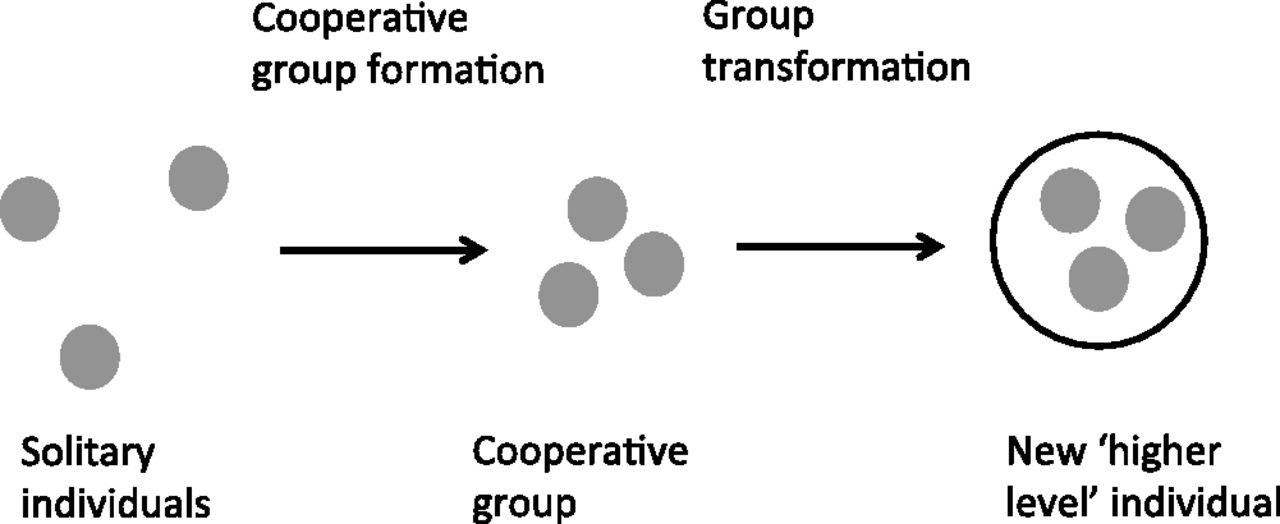
\includegraphics[width=\linewidth]{static/transition-west2015.jpg}
%     \end{subfigure}
    \tikz{            
    \node[accion] (i1) {} ;
    \node[accion, yshift=0.6cm, xshift=0.4cm] (i2) {} ;
    \node[accion, yshift=0.6cm, xshift=-0.4cm] (i3) {} ;
    \node[const, yshift=0.3cm, xshift=0.4cm] (i) {};
    
    \node[const, yshift=-0.8cm] (ni) {$\hfrac{\text{Individuos}}{\text{solitarios}}$};
    
    \node[const, yshift=1.2cm, xshift=1.5cm] (m1) {$\hfrac{\text{Formación}}{\text{de grupos}}$};
    
    \node[const, right=of i, xshift=2cm] (c) {};
    \node[accion, below=of c, yshift=0.35cm, xshift=0.4cm] (c1) {} ;
    \node[accion, above=of c, yshift=-0.35cm, xshift=0.6cm] (c2) {} ;
    \node[accion, above=of c, yshift=-0.35cm, xshift=0.2cm] (c3) {} ;
    \node[const, right=of c, xshift=0.6cm] (cc) {};
    
    \node[const, right=of ni, xshift=1.3cm] (nc) {$\hfrac{\text{Grupos}}{\text{cooperativos}}$};

    \node[const, right=of m1, xshift=1.2cm] (m2) {$\hfrac{\text{Transición}}{\text{mayor}}$};
    
    \node[const, right=of cc, xshift=2cm] (t) {};
    \node[accion, below=of t, yshift=0.35cm, xshift=0.4cm] (t1) {} ;
    \node[accion, above=of t, yshift=-0.35cm, xshift=0.6cm] (t2) {} ;
    \node[accion, above=of t, yshift=-0.35cm, xshift=0.2cm] (t3) {} ;
    
    \node[const, right=of nc, xshift=1.1cm] (nt) {$\hfrac{\text{Unidad de}}{\text{nivel superior}}$};

    \edge {i} {c};
    \edge {cc} {t};
    
    \plate {transition} {(t1)(t2)(t3)} {}; %
    }
    \caption{Transiciones evolutivas mayores}
    \label{fig:transitions}
\end{figure}

\en{Some of the paradigmatic transitions are: from prokaryotic to eukaryotic cells; from protozoa to animals, plants and fungi (cell differentiation and emergence of multicellular organisms); and from solitary individuals to societies. }%
\es{Algunas de las transiciones paradigmáticas son: de las células procariotas a las eucariotas; de los protozoa a los animales, plantas y hongos (diferenciación celular y emergencia de organismos multicelulares); y la formación de comunidades. }%
%
\en{From that moment until now, life has acquired an extraordinary complexity, both in terms of cooperation and specialization. }%
\es{Desde su origen hasta ahora, la vida adquirió una extraordinaria complejidad, tanto a nivel de cooperación como de especialización. }%
%
\begin{figure}[ht!]
    \centering
    \begin{subfigure}[b]{0.5\textwidth}
    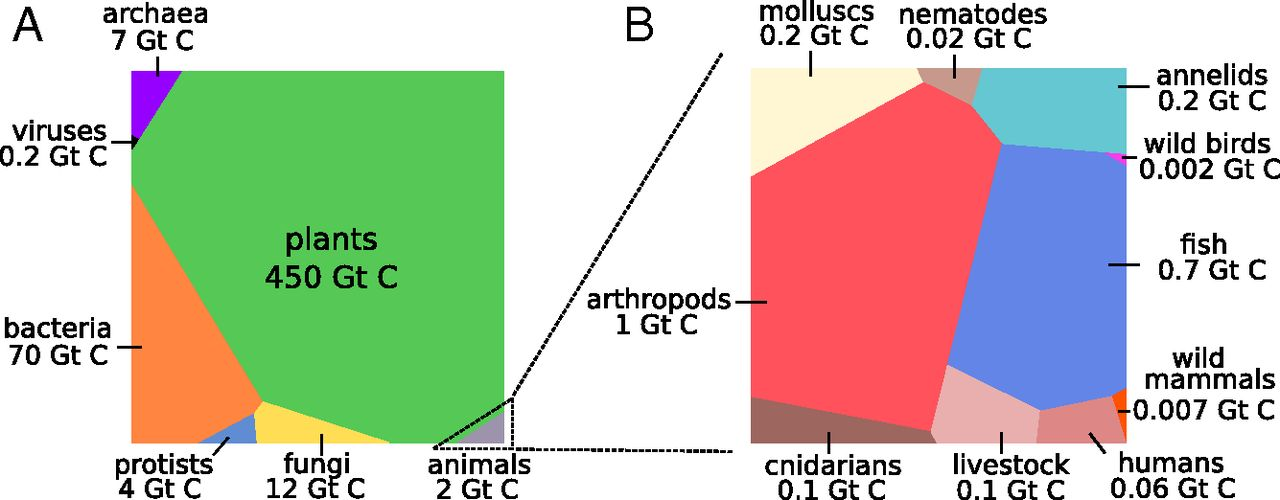
\includegraphics[width=\linewidth]{static/biomass.jpg}
    \end{subfigure}
    \caption{
    \en{Distribution of biomass on Earth estimated by Bar-On et al.~\cite{barOn2018-biomass}. }
	\es{Distribución de la biomasa en la Tierra estimada por Bar-On et al.~\cite{barOn2018-biomass}. }%
    }
    \label{fig:biomass}
\end{figure}
%
En la actualidad, el 82\% de la biomasa corresponde al reino de las plantas, el 13\% a las bacterias, el 2.2\% a los hongos, y 0.36\% a los animales, dentro de los cuales los humanos representamos el 3\%.
%
No es sorprendente que la plantas ocupen la mayor proporción de la biomasa, pues ellas son las principales productoras primarias, capaces de generar materia orgánica a partir de la luz solar, el agua y los gases de la atmósfera.
Las plantas realizan este complejo proceso de forma sumamente eficiente.
Este conocimiento está almacenedado en su material genético, y no existe conocimiento científico-técnico que sea capaz de imitar este proceso.
Los animales, hongos y el resto de heterótrofos, están obligados a adquirir el material orgánico de otros seres vivos, lo que los obliga a coexistir con sus presas, creando una compleja red de dependecias mutuas que constituyen la unidad de nivel superior mayor, los sistemas ecológicos.

\section{Cultura}

La especial integraci\'on de los procesos biol\'ogicos, cognitivos y sociales que permiten a los humanos desarrollar culturas complejas se debió a una coevolución genético-cultural desencadenada por el desarrollo previo de la crianza cooperativa~\cite{hrdy2020-emotionallyModern}.
La forma en la que estos homininos organizaron la crianza produjo un ambiente que favoreció la selección de jóvenes capaces de monitorear y comprender las intenciones de los demás, y de trasmitir a sus cuidadadores sus propias necesidades.
%A diferencia de nuestros parientes más cercanos (chimpancés, bonobos, gorilas y orangutanes)
Antes del surgimiento de los humanos anatómicamente modernos (masa cerebral actual) y de los humanos conductualmente modernos (lenguaje), surgió en África una linaje emocionalmente moderno con capacidades para el entendimiento mutuo~\cite{hrdy2020-emotionallyModern}.

La comprensión mutua, la imitación y el lenguaje permitieron la  transmisión de conocimientos basados en la experiencia de otros (\emph{aprendizaje social}), dando inicio a un proceso cooperativo inter-generacional que produjo el desarrollo de \emph{las culturas}, sistemas de información independiente al genético que permitió a las poblaciones humanas adaptarse rápidamente a los cambiantes contextos ambientales.
El surgimiento de este nuevo sistema de información produjo cambios radicales para nuestra especie.
Antes de la transición cultural, estuvimos en grave peligro de extinción, lo que se evidencia en la baja diversidad del genoma humano.
Luego de la transición cultural, organizados en sociedades cazadores-recolectores, nuestra especie fue capaz de ocupar en pocos años todos los nichos ecológicos de la tierra como ningún otro vertebrado terrestre lo había logrado antes.
Saliendo de África ocupamos Asia, Oceanía y las Américas (Figura~\ref{fig:agricultura}).
% La información transgeneracional fue la que le permitió a estas sociedades simples adaptarse rápidamente a los nuevos desafíos ecológicos.

\begin{figure}[ht!]
    \centering
    \begin{subfigure}[b]{0.6\textwidth}
     \includegraphics[width=\textwidth]{figures/agricultura.pdf}
     \label{fig:agricultura}
    \end{subfigure}
%     \begin{subfigure}[b]{0.40\textwidth}
%     \includegraphics[width=\textwidth]{static/polynesia.png} 
%     \caption{Poblamiento del océano Pacífico}
%     \label{fig:polynesia}
%     \end{subfigure}
    \caption{
    Poblamiento humano (flechas) y surgimientos independientes de la agricultura (puntos).
    Proyección políedrica que conserva los tamaños relativos de la tierra.
    %Las felchas indican el poblamiento, desde África a Asia, y de Asia hacia Oceanía y América.
    %Los puntos rojos indican surgimiento independiente de agricultura.
    %El mapa de la figura~\ref{fig:polynesia}, desarrollado por Thorsby~\cite{thorsby2016-polynesiaAmerica}, muestra el poblamiento de la Polynesia y los contactos con Ámerica evidenciados en el material genéticos.
    }%
    \label{fig:poblamiento}
\end{figure}

El cambio cultural es un fenómeno poblacional que emerge como consecuencia del intercambio de información entre individuos.
%
\en{Based on the principles of evolutionary theory (descent, mutation and selection), a theoretical framework of ``cultural evolution'' has been developed to explain how culture changes over time. }%
\es{Basada en los principios de la teoría de la evolución (descendencia, modificación y selección), se ha desarrollado un marco teórico de \emph{evolución cultural} que intenta explicar cómo cambia la cultura en el tiempo. }%
%
\en{Descent, mutation and selection of cultural information occurs when an individual adopts the behavior of others, either because it is the behavior of the majority (frequency-based strategy) or because the other individual is particularly successful or prestigious (payoff-based strategy). }%
\es{La descendencia, mutación y selección de la información cultural se produce cuando una persona adopta el comportamiento de otras, sea porque es el comportamiento de la mayoría o sea porque es la otra persona es particularmente exitosas o prestigiosas. }%
%
\en{All social learning processes modify to some degree the cultural variant adopted. }%
\es{Todos los procesos de aprendizaje social modifican en algún grado la variante cultural adoptada. }%
%
\en{And some of these cultural variants spread faster or are more stable than others, predominating over time. }%
\es{Y algunas de esas variantes culturales se propagan más rápido o son más estables que otras, predominando en el tiempo. }%

% Parrafo

La experiencia acumulada a través de las generaciones por las más diversas comunidades del mundo condujo, de forma independiente, al desarrollo de tecnologías de reciprocidad sorprendentemente similares entre sí.
%
La antropología ha reconocido la existencia de una obligación universal de dar y de recibir.
%
De esta forma, el acto de donar, dar un regalo o hacer un favor activa un ciclo de intercambios a través de la obligación recíproca para devolver de alguna forma lo recibido.
%
Este tipo de intercambios es la primera forma económica y es un mecanismo de flujo de bienes y servicios fundamental incluso en las sociedades modernas, a través de las que se establecen relaciones de correspondencia, hospitalidad, protección y asistencia mutua~\cite{mauss, polanyi, salins}.

% Parrafo

Si bien los intercambios recíprocos ocurren generalmente de forma rutinaria, en todas las sociedades se pueden reconocer dos mecanismos que cumplen la función de re-ciclar los v\'inculos interprersonales: los ritos festivos y los ritos coercitivos~\cite{segato2016-guerraContraLasMujeres}.
%
Los ritos coercitivos, no son otra cosa que ceremonias para la reactivación de flujos de intercambios rotos previamente por conflictos entre partes.
%
Están orientados el restablecimiento de los vínculos mediante los mecanismos de ``reparación'', ``conciliación'' y ``ayuda'' \cite{zaffaroni2013-cuestionCriminal}, nombre relativamente arbitrarios para los tres tipos de intercambios posibles entre partes: dar ($\rightarrow$), intercambiar ($\leftrightarrow$) y recibir ($\leftarrow$).
%
La expulsión del agresor de la comunidad sólo se prevee en casos extremadamente excepcionales, pues el primer derecho de sus miembros es formar parte de la comunidad \cite{segato2016-guerraContraLasMujeres}.

% Parrafo

Las tecnologías de reciprocidad social son fundamentales para la supervivencia de las comunidades en el tiempo, pues ellas reducen las fluctuaciones individuales que ponen en peligro su estabilidad.
%
La teoría de la probabilidad nace en 1648 justamente como respuesta a la pregunta de cuál es el \emph{precio justo} en contextos de incertidumbre.
%
El problema analizaban Pascal y Fermat en sus cartas es equivalente al siguiente.
%
Tiramos dos veces la moneda.
%
Si sale seca $S$ en la primera y en la segunda, una persona (en rojo) le hace un favor a la otra.
%
En caso contrario, el favor se invierte.
%
¿Cuál es el valor justo de la reciprocidad en este contexto de incertidumbre?

\begin{figure}[ht!]
    \centering
    \tikz{
    \node[latent, draw=white, yshift=0.7cm, minimum size=0.1cm] (b0) {};
    \node[latent,below=of b0,yshift=0.7cm, xshift=-1cm] (r1) {$S$};
    \node[latent,below=of b0,yshift=0.7cm, xshift=1cm] (r2) {$C$};

    \node[latent, below=of r1, draw=white, yshift=0.8cm, minimum size=0.1cm] (bc11) {};
    \node[accion, below=of r2, draw=white, yshift=0cm, color=blue!70] (bc12) {};
    \node[latent,below=of bc11,yshift=0.8cm, xshift=-0.5cm] (r1d2) {$S$};
    \node[latent,below=of bc11,yshift=0.8cm, xshift=0.5cm] (r1d3) {$C$};

    \node[accion,below=of r1d2,yshift=0cm, color=red!70] (br1d2) {};
    \node[accion,below=of r1d3,yshift=0cm, color=blue!70] (br1d3) {};
    \edge[-] {b0} {r1,r2};
    \edge[-] {r1} {bc11};
    \edge[-] {r2} {bc12};
    \edge[-] {bc11} {r1d2,r1d3};
    \edge[-] {r1d2} {br1d2};
    \edge[-] {r1d3} {br1d3};
    }
    \caption{El problema del \emph{valor justo} que da inicio a la teoría de la probabilidad}
    \label{fig:pascal-fermat}
\end{figure}

La respuesta a la que arribaron Pascal y Fermat es que el valor de los favores tiene que ser inversamente proporcional a la probabilidad de hacer el favor.
%
Si la moneda es no sesgada, hay 1/4 de probabilidad de que salgan dos secas (terminal roja), 1/4 de que salga seca en la primera y cara en la segunda (terminal azul) y 1/2 de que salga cara en la primera (terminal azul).
%
Luego, la probabilidad de que la persona azul haga un favor es 3/4.
%
Si la persona roja hace favores por un valor equivalente a 4, el azul tiene que devolver los favores con un valor de 4/3, una relación de 3 a 1.
%
Esta forma intuitiva de calcular la probabilidad de un conjunto de eventos mutuamente excluyentes, como suma de sus probabilidades elementales, constituye el axioma fundamental de Kolmogorov a partir del cual se puede montar toda la teoría de la probabilidad.

% Parrafo

De forma similar a las tecnologías de reciprocidad social, las tecnologías de reciprocidad ecológica promueven la coexistencia con las especies de las cuales dependemos garantizando así la supervivencia de la comunidad en el tiempo.
%
Los estudios comparados indican que las instituciones capaces de interactuar de forma estable con los sistemas ecológicos siempre son de tipo comunitario, basados en normas que condensan la acumulación conocimiento experto resultado de un largo proceso inter-generacional de evolución cultural local~\cite{ostrom1990}.
% 
El remplazo repentino de estos sistemas culturales locales por instituciones modernas externas, privadas o públicas, produce generalmente desequilibrios en los sistemas ecológicos por sobre explotación de los recursos, reduciendo el tamaño máximo de población que el ambiente puede soportar~\cite{ostrom2010}.

% Parrafo

Los pueblos bien adaptados para la coexistencia intercultural y ecológica practican cosmovisiones basadas en lógicas paraconsistentes que les permite creer en A y no A al mismo tiempo.
Estas cosmovisiones, que obligan a no rechazar ninguna alternativa aunque se tenga preferencia por alguna, son la base de toda tecnología de reciprocidad con la biocenosis en todo el mundo, como son los ritos \emph{Canang sari} practicados en Bali o como los ritos \emph{pachamámicos} practicados en América del sur.
\begin{figure}[ht!]
    \centering
    \begin{subfigure}[b]{0.45\textwidth}
    \centering
    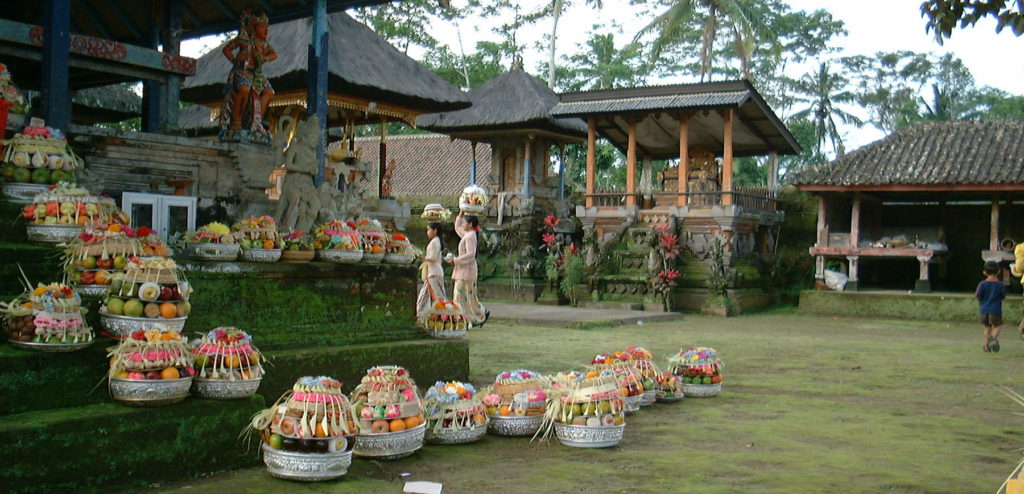
\includegraphics[width=\linewidth]{static/bali-offerings}
    \caption{Canang sari}
    \label{}
    \end{subfigure}
    \begin{subfigure}[b]{0.3\textwidth}
    \centering
    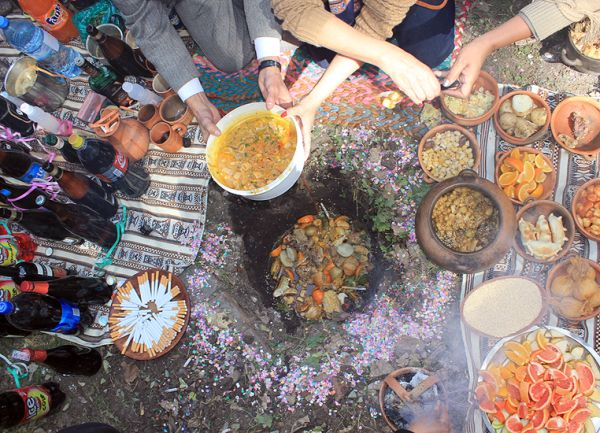
\includegraphics[width=\linewidth]{static/pachamama}
    \caption{Pachamama}
    \label{}
    \end{subfigure}
    \caption{Tecnologías de reciprocidad socio-ecológicas.}
    \label{fig:mito}
\end{figure}
Estas cosmovisiones basadas en lógicas paraconsistentes obliga al ser humano a fomentar la coexistencia con otras formas de vida, como con otras culturas.

% Parrafo

Las tecnologías de reciprocidad ecológica produjeron la aparición independiente de la domesticación de especies animales y vegetales, el desarrollo de caracteres genéticos especiales que surgen como resultado de una interacción prolongada entre las especies.
%
En particular, la reciprocidad con las especies fotosintéticas (\emph{agricultura}), únicas con la capacidad de producir materia orgánica a partir del sol y la materia inorgánica, produjo nuevamente cambios radicales para nuestra especie.
%
La agricultura impulsó un marcado aumento poblacional.
%
Y el aumento de la población promovió, a su vez, el desarrollo de nuevas innovaciones tecnológicas y científicas, como la escritura, la matem\'aticas, las ingenier\'ias, la astronomía, las ciencias políticas, entre otras.

% Parrafo

La agricultura surgió de manera de forma paralela en los seis grandes sistemas geográficos de la tierra: en la región central de África subsahariana, en Asia occidental, en Asia oriental, en Oceanía norte, en América del norte y en América del sur (las puntos rojos de la figura~\ref{fig:agricultura}).
%
Alrededor de estos puntos se desarrollaron los principales centros poblacionales de la humanidad.
%
Durante el año 1400 el mundo florecía de sociedades "prósperas"~\cite{dussel2004-sistemaMundo}: Aztecas en Ámerica del norte, Incas en Ámerica del sur, Tongas en el Pacífico, Bantúes en África sub-sahariana, los Árabes e Indios en Asia occidental y Chinos en Asia oriental, por mencionar algunos.
%
El desarrollo tecnológico de todas estas sociedades fue extraordinario. 
%
% El imperio de Tonga ocupaba hace siglos todo el oc\'eano Pac\'ifico (figura~\ref{fig:polynesia}) con tecnologías de navegación que le habían permitido tener intercambios con América de Sur~\cite{thorsby2016-polynesiaAmerica, ioannidis2020-polynesiaAmerica}.
% %
% En América del Sur se había desarrollado un sistema de intercambios basado en la reciprocidad de trabajo (minka, ayni y mita) que le permitía a las comunidades administrar eficientemente el uso de los bienes comunes y al Estado desarrollar la infrastructura en el vasto territorio montañoso~\cite{murra1978-organizacion}.
% %
% En la región Azteca se había desarrollado un extenso mercado regional con ciudades de hasta 300.000 habitantes, tres veces la ciudad de Venecia en esa misma época.%~\cite{www7.uc.cl}. %http://www7.uc.cl/sw_educ/historia/conquista/parte1/html/h54.html
% %
% El mundo \'Arabe comerciaba productos desde el Océano Pacífico, en las Filipinas, hasta el Oc\'eano Atl\'antico, en Marruecos, conectando las innovaciones culturales de distintos hemisferios del planeta~\cite{dussel2004-sistemaMundo}.
% %
África siempre fue el continente más diverso cultural y genéticamente, pero quizás el centro más innovador en términos científicos y tecnologías haya sido la región de China~\cite{needham2004-generalConclusionsAndReflections}.

% Parrafo

\section{Ciencia y evolución cultural}

John Needham, el británico que dedicó su vida a recopilar la monumental historia científica y técnica de China, reconoce que comenzó a estudiar el tema motivado por responder la pregunta de por qué sólo Europa occidental había logrado el avance científico.
\begin{quotation}
When I first formed the idea, about 1938, (...) I regarded the essential problem as that of why modern science had not developed in Chinese civilisation (or Indian or Islamic) but only in that of Europe~\cite{needham2004-generalConclusionsAndReflections}.%
\end{quotation}
Luego de 60 años de investigaciones, Needham se ve obligado inviertir la pregunta.
\begin{quotation}
Why, between the -1th century and the 15th century, was Chinese civilisation much \emph{more} efficient than occidental in gaining natural knowledge and in applying it to practical human needs?~\cite{needham2004-generalConclusionsAndReflections}
\end{quotation}

% Parrafo

Desde Hegel hasta la fecha, las explicaciones eurocéntricas intentan explicar la proposperidad actual de occidente a través de una causa interna: la ``ética protestante'' de Max Weber~\cite{weber1905-eticaProtestante}, la ``mentalidad burguesa'' de José Luis Romero~\cite{romero1967-revolucionBurguesa}, o más recientemente el ``sistema de parentezco'' de Joseph Henrich~\cite{henrich2020-weirdest}.
La paradoja que no puede responder la fábula eurocéntrica es cómo una sociedad sumida en un proceso de involución cultural único, como la sociedad feudal de la ``edad media'', pudo generar de repenten el extraordinario proceso de desarrollo científico y técnico de la modernidad.

% Parrafo

Así como la integración favorece los proceso de innovación y acumulación cultural, el asilamiento induce pérdidas masivas de información cultural.
%
Un ejemplo paradigmático de aislamiento total ocurre con la separación de Tasmania del continente Australiano por la subida del nivel del mar ocurrida a comienzos del Holonceno.
%
La evidencia arqueológica y etnohistórica indica que desde el principio del Holoceno las sociedades de Tasmania perdieron gran parte de su cultura tecnológica.
La principal hipótesis sugiere que la reducción del tamaño efectivo de la población fue la causa de la pérdida cultural~\cite{Henrich2004}.
%
La capacidad de almacenamiento (e innovación) de tecnologías complejas, incluso aquellas desarrolladas por las sociedades cazadoras-recolectoras, requiere de un tamaño mínimo de la población que sólo se puede alcanzar a través de la coexistencia entre distints pueblos con identidad propia.

% Parrafo

Un caso de asilamiento parcial ocurre en Europa occidental durante la Edad Media.
%
Antes de que tuviera lugar la Edad Media, el Imperio Romano produjo una pérdida masiva de diversidad cultural en su entorno, que tuvo consecuencias críticas para esta sociedad.
%
Arrinconada ya en el lejano occidente por el fr\'io polar y la falta de tecnolog\'ias de navegaci\'on del Atlántico, Europa occidental comienza en el siglo octavo a quedar paulatinamente aislada del ``sistema mundo'' por la expansión Árabe al sur y por la serie cismas con el Imperio Romano de Oriente~\cite{Dussel}.
%
Aislada pacialmente del sistema mundo, esta sociedad entra en un proceso de involución cultural que condujo a un deterioro extremo de las condiciones de vida.

\begin{figure}[ht!]     
  \centering 
  \begin{subfigure}[c]{0.45\textwidth}
    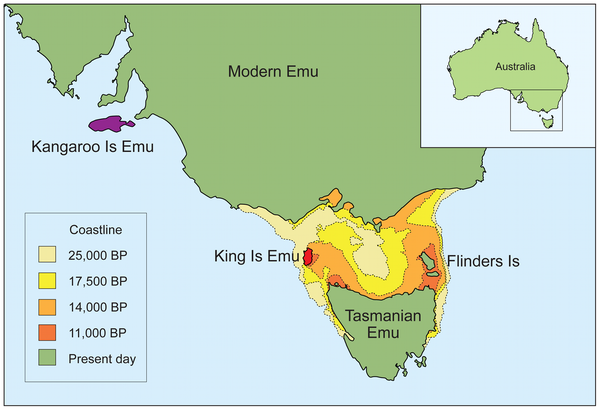
\includegraphics[width=\textwidth]{static/tasmania.png} 
    \caption{Tasmania}
    \label{fig:tasmania}
  \end{subfigure}
  \begin{subfigure}[c]{0.45\textwidth}
    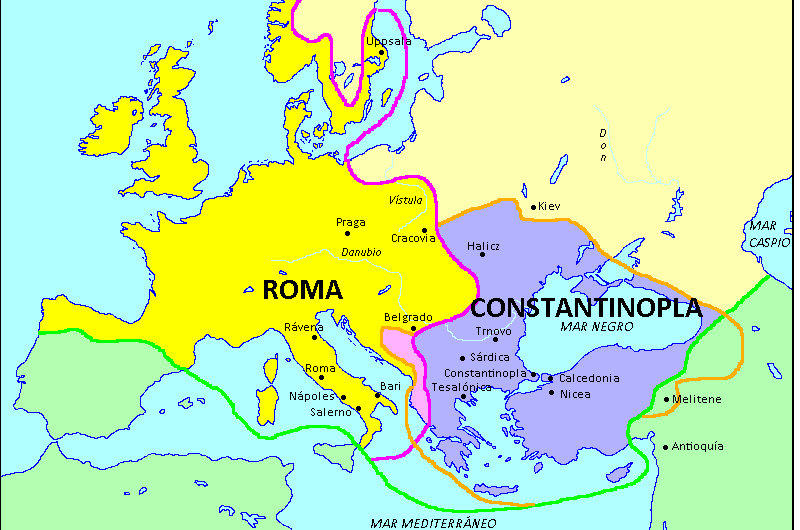
\includegraphics[width=\textwidth]{static/cisma.png} 
    \caption{Edad media}
    \label{fig:cisma}
  \end{subfigure}
  \caption{Aislamiento}
  \label{fig:aislamiento}
\end{figure}

En la etapa de aislamiento comenzó a ganar terreno al interior de la sociedad feudal el criterio de autoridad (religiosa, militar, académica, económica, sexual) como fundamento del ``saber auténtico''.
A pesar de la involución cultural generalizada, durante la Edad Media las instituciones heredadas del Imperio Romano de Occidente, en cabeza de la Iglesia Católica Romana, comenzaron a competir con las comunidades indígenas locales y a producir una conjunto de novedosas tecnologías de colonización~\cite{zaffaroni2013-cuestionCriminal}.
La primera y más importante fue la regulación de las relaciones comunitaria de reproducción (matrimonios) de forma más detallada que la propiedad.
Se proscribe así el rol político que las mujeres desempeñan en el espacio doméstico comunitario, interviniendo en el funcionamiento de sus tecnologías de sociabilidad.

% Parrafo

%El avance colonial estuvo (y está) motivado principalmente por una deficiencia social más que por una puramente material.
La población desertora de las comunidades que pierden el arraigo comunitario pasan a sumarse como mano de obra para las actividades militares contra otros pueblos.
El mandato universal de exhibir públicamente alguna forma de poder para adquirir el estatus masculino hizo que los hombres derrotados se volvieran vulnerables al ejemplo de las masculinidades victoriosas.
Con el debilitamiento de los vínculos comunitarios, la cosmovisión colonial e instrumental logra introducirse, cosificando todas las formas de vida.

% Parrafo

El poder punitivo se fue extendiendo y un nuevo sistema penal re-nació de los llamados \emph{libris terribilis} del Digesto, antiguas leyes romanas recolectadas por encargo del emperador Justiniano de Constantinopla pero re-interpretadas en occidente de modo de liberar al poder punitivo de todo límite.
En esta etapa, el sujeto masculino se torna modelo de lo humano y de todo cuanto sea dotado de politicidad, interés general y valor universal, y el espacio de las mujeres se transforma en margen y resto de la política.
La guerra contra las mujeres se formaliza definitivamente con la publicación del \emph{Malleus maleficarum} en 1484, que será el segundo best seller después de la Biblia durante los siguientes 200 años.

% Parrafo

% Producto de la pésima situación socio-económica, la sociedad fedual intenta varias veces, sin éxito, recuperar la integración al sistema mundo por el oriente.
% Por lo tanto, la única opción que quedaba era explorar los mares del este.
% Había mejores tecnologías de navegación en el mundo Árabe, en China y en el imperio de Tonga.
% Pero a diferencia de esos casos, apenas la sociedad fedual logra navegar el Atlántico, se desata un proceso migratorio típico de cualquier sociedad sumida en un proceso de grave violencia interna.
% El flujo migratorio europeo hacia américa comienza a finales del siglo 15 y termina recién a mediados del siglo 20.

Producto de la pésima situación socio-económica, apenas Europa occidental logra navegar el Atlántico, comienza un proceso migratorio típico de cualquier sociedad sumida en un proceso de grave violencia interna y degradación social, un flujo migratorio que comienza a finales del siglo 15 y termina recién a mediados del siglo 20.
%Además de la buena predisposición con la que los exploradores reportan haber sido recibidos por los habitantes Americanos, l
La llegada de masiva de emigrantes feudales produjo una serie de pandemias en América que redujeron la población local en al menos un 66\% entre los años 1500 y el 1600~\cite{koch2019-europeanArrival}.
Un siglo antes, China hab\'ia incorporado la plata como monedad oficial, la que ya estaba siendo utilizada en todo el mundo Árabe~\cite{pomeranz2000-divergence, pomeranz2018-tradeCreated}.
El Estado Incaico, que estaba organizado en base a un sistema de intercamios reciproicitarios no monetarios, se encontraba era una región montañosa rica en plata.
Cuando 1546 los exploradores descubren la montaña de plata de Potosí, en el centro del sistema estatal incaico, la Europa feudal queda inmediatamente en una posición de privilegio en todo el mundo afro-euro-asiático.

% Parrafo

El acceso a la plata americana produce un giro geopolítico.
La sociedad feudal rompe el cerco que la tenía asilada del sistema mundo 25 años después de haber descubierto la montaña de plata de Potosí, y 80 años después de haber logrado navegar el Atlántico, en la batalla de Lepanto.
La plata, que ya era reconocida como moneda oficial en todo el mundo eruo-asiático, colocó de repente a esta sociedad marginal en una situación de integración privilegiada al sistema mundo.
La plata de América fluye en todas las direcciones, principalmente en dirección a China, y se inicia un proceso rápido de acumulación cultural basado en las tecnologías extranjeras.
%El proceso de involución cultural producto del asilamiento al sistema mundo durante la Edad Media, dio lugar a un proceso de rápidas innovaciones científicas y técnicas a partir de la integración privilegiada generada por el acceso a la plata, moneda de cambio en todo el continente afro-euro-asiático.

% Parrafo

\begin{figure}[ht!]     
  \centering 
  \begin{subfigure}[b]{0.48\textwidth}
    
\includegraphics[width=\textwidth]{static/plata-potosi} 
    \caption{Plata}
    \label{fig:potosi}
  \end{subfigure}
   \ \ 
  \begin{subfigure}[b]{0.47\textwidth}
    \includegraphics[width=\textwidth]{figures/china.pdf} 
   \caption{Opio}
    \label{fig:china-pop}
  \end{subfigure}
  \caption{La plata y el opio como las llaves de la integración privilegiada de la Europa occidental en el sistema mundo.}
  \label{fig:integracion}
\end{figure}

% Parrafo

Durante 250 años la plata americana sirvió para muchas cosas, pero principalmente para comprar productos chinos que impulsan la primera industrialización británica.
Europa consumía productos asiáticos, pero exportaba muy poco a Asia.
El comercio internacional de opio comenzó a mediados del 1700 como respuesta a una crisis del comercio internacional europeo, especialmente británico.
El opio, un producto lujoso utilizado en China como medicina (raramente como estupefaciente), fue prohibida por los emperadores chinos en 1729, que por su abundancia hacía crecer lentamente la cantidad de adictos.
Las consecuencias fueron más graves cuando en 1818 se desarrolla una mezcla de opio más barata y potente.

% Parrafo

Mediante el narcotráfico Europa occidental consigue por primera vez, recién en el siglo 19, revertir el déficit comercial que históricamente tuvo con China.
El número de adictos llegó a ser lo suficientemente alarmante, y en 1839 China comete el error de declarar la guerra al narco-estado británico en su propio territorio.
Los resultados fueron terribles.
No sólo no pudieron impedir el ingreso de la droga.
Perdieron también su autonomía arancelaria, el derecho a someter a los residentes extranjeros a la ley China.
Expuesta a su debilidad militar, China sufrió un siglo calamitoso de agresiones extranjeras, desorden interno y guerra civil, que produjo una caída de 1/5 de su población (figura~\ref{fig:china-pop}).

% Parrafo

Luego de la derrota de China por parte del narco-estado británico, se establece por pimera vez la hegemonía de Europa occidental en el sistema mundo y comienza un proceso de colonización en todo el mundo.
%, que hasta el momento estaba limitado a América continental estaba limitada a puertos e islas.
En 1850 comienza la colonización de África continental y de los extensos territorios americanos que todavía seguían a manos de comunidades locales.
Comienza la era de los genoentocidios.
\begin{figure}[ht!]
    \centering
    \begin{subfigure}[b]{0.48\textwidth}
    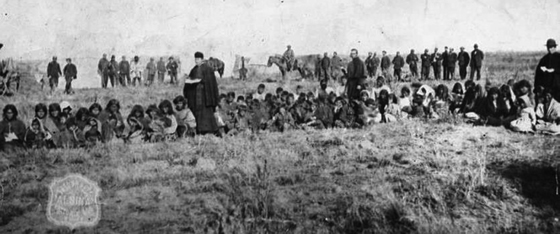
\includegraphics[width=\linewidth]{static/genocidio_patagonia}
    \caption{Genoetnocidios}
    \label{fig:genocidio_patagonia}
    \end{subfigure}
    \begin{subfigure}[b]{0.47\textwidth}
    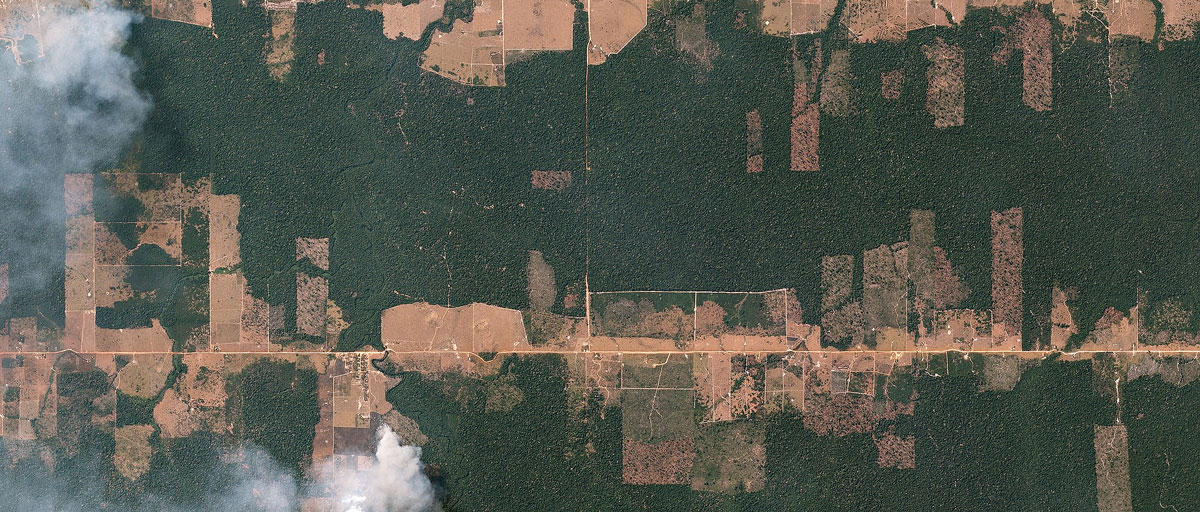
\includegraphics[width=\linewidth]{static/deforestation-brazil}
    \caption{Crisis ecológica}
    \label{fig:deforestation-brazil}
    \end{subfigure}
    \caption{
    La masiva pérdida de diversidad cultural trajo como consecuencia la masiva pérdida de biodiversidad actual, una crisis ecológica sin precedentes.
    }
    \label{fig:cultural-lose}
\end{figure}
En todas las partes del globo, los exploradores y etnógrafos fueron documentando la perdida de cultural debida al avance del frente colonial-moderno, estatal o privado, sobre las autonomías locales.
Es una nueva era de avances científicos y tecnológicos, pero por otro es la era de pérdida de diversidad cultural.
A pesar de todos los avances científicos, la ciencia metropolitana moderna no fue capaz de compensar la pérdida de los conocimientos milenarios acumulados por las comunidades autónomas locales.
La masiva pérdida de diversidad cultural trajo como consecuencia la masiva pérdida de biodiversidad actual, una crisis ecológica sin precedentes (figura~\ref{fig:deforestation-brazil}).
%Quizá la coexistencia sea la única estrategia evolutivamente estable, y quienes la rompan sufran tarde o temprano las consecuencias.

% Parrafo

\section{La ventaja de la cooperación y la especialización}


\en{In evolution it is said that the growth of a lineage over time, $\omega(t)$, is governed by a stochastic sequence of survival and reproduction rates $f(\cdot)$ dependent on a random environment $\Aa$, }
\es{En evolución se dice que el crecimiento de un linaje en el tiempo, $\omega(t)$, esta gobernado por una secuencias de tasas de supervivencia y reproducción $f(\cdot)$ dependientes de un ambiente aleatorio $\Aa$, }%
%
\begin{equation} \label{eq:modelo_exponencial}
\omega(T) = \prod_t^T f(\Aa(t)) \approx g^T
\end{equation}
%
\en{where $\Aa(t)$ represents the state of the environment at time $t$ and $g$ represents the characteristic growth rate when $T$ is sufficiently large. }%
\es{donde $\Aa(t)$ representa el estado del ambiente en el tiempo $t$ y $g$ representa la tasa de crecimiento caracterísitica cuando $T$ es suficientemente grande. }%
%
Podemos interpretar $\omega(T)$ como el tamaño de una población en el tiempo, pero también esa población puede ser un recurso para otro linaje.
%
Por eso, de aquí en adelante hablaremos de recursos, pero hay que mantener la idea de que este es un proceso al que están sujeto el crecimiento de los linajes en general.
%
\en{For example, suppose nature flips a coin, if it comes up heads the population reproduces 50\% and if it comes up tails it survives 60\%. }%
\es{Por ejemplo, supongamos que la naturaleza lanza una moneda, si sale cara los recursos crecen 50\% y si sale seca perdemos 40\%. }%
\begin{equation} \label{eq:estrategia_base}
f(\Aa) =
\begin{cases}
 1.5 & \Aa = \text{ \en{Head}\es{Cara} } \\
 0.6 & \Aa = \text{ \en{Tail}\es{Seca} }
\end{cases}
\end{equation}
%
\en{A similar example was proposed by Lewontin and Cohen (1969)~\cite{lewontin1969-randomlyVaryingEnvironment}. }%
\es{Un ejemplo similar fue anlizado por Lewontin y Cohen (1969)~\cite{lewontin1969-randomlyVaryingEnvironment}. }%
%
% \en{Different strategies $\Ee$ can be described with different functions $f_\Ee(\Aa)$. }%
% \es{Diferentes estrategias $\Ee$ las podemos describr con diferentes funciones $f_\Ee(\Aa)$. }%
% %
% \en{According to the standard model of evolution, known as \emph{replicator dynamic} \cite{taylor1978-replicatorDynamic}, the change in the proportion of a strategy in the population, $x_\Ee$, is determined by its characteristic growth rate $g_\Ee$, }%
% \es{Según el modelo estándar de evolución, conocido como \emph{replicator dynamic} \cite{taylor1978-replicatorDynamic}, el cambio de la proporción de una estrategia en la población, $x_\Ee$, está determinado por su tasa de crecimiento caracterísitica $g_\Ee$, }%
% % schuster1983-replicatorDynamics, hofbauer2003-evolutionaryGameDynamics
% %
% \begin{equation} \label{eq:replicator_dynamic}  \tag{Replicator dynamic}
% \hspace{3cm} x_\Ee^\prime = \frac{x_\Ee g_\Ee}{\sum_i x_i g_i}
% \end{equation}
% %
% \en{where the denominator acts as a normalization constant. }%
% \es{donde el denominador actúa como constante de normalización. }%
% %
\en{But, what is the characteristic growth rate $g$? }%
\es{¿Cuál es la tasa de crecimiento característica $g$ en este caso? }%
%
\en{Much of the evolutionary literature considers that the correct estimate is obtained by the expected value, $g^t = \langle \omega \rangle_t$. }%
\es{Buena parte de la literatura en evolución considera que la estimación correcta se obtiene mediante el valor esperado, $g^t = \langle \omega \rangle_t$. }%
%
\begin{equation}
\langle \omega \rangle_t = \sum_{\omega \in \Omega_t} \omega \cdot  P(\omega)
\end{equation}
%
\es{Donde $\Omega_t$ es el conjunto de todas las posibles estados de $\omega$ en el tiempo $t$, y $P(\omega)$ es la la probabilidad de que el estado $\omega$ ocurra. }%
% 
\en{In the coin example, the expected value in the first two time steps is, }%
\es{En el ejemplo de la moneda, el valor esperado en los dos primeros pasos temporales es, }%
%
\begin{equation}
\begin{split}
\langle \omega \rangle_1 & = 1.5 \cdot \frac{1}{2} + 0.6 \cdot  \frac{1}{2} = 1.05 \\ 
\langle \omega \rangle_2 &=  1.5^2 \cdot \frac{1}{4} + 2 (0.6 \cdot 1.5 \cdot \frac{1}{4} ) + 0.6^2 \cdot \frac{1}{4}= 1.05^2
\end{split}
\end{equation}
%
\en{That is, the estimated growth rate according to the expected value is $5\%$ for each time step, $\langle \omega \rangle_t = 1.05^t$. }%
\es{Es decir, la tasa de crecimiento estimada según el valor esperado es de $5\%$ por cada paso temporal, $\langle \omega \rangle_t = 1.05^t$. }%
%
\en{And indeed that is what happens with the average of several individual trajectories, $\omega(t)$. }%
\es{Y efectivamente eso es lo que ocurre con el promedio de varias trayectoria individuales, $\omega(t)$. }%
%
\begin{figure}[ht!]
    \centering
    \begin{subfigure}[b]{0.45\textwidth}
    \includegraphics[width=\linewidth]{figures/pdf/ergodicity_expectedValue.pdf}
    \end{subfigure}
    \caption{
    \es{Promedio de los recursos (en escala logarítimica) a medida que aumentamos la cantidad de trayectorias individuales incluidas en el promedio (de $10^0$ a $10^4$). }%
    %
    \es{Cuando la cantidad de trayectorias individuales incluidas en el promedio es suficientemente grande, el promedio es igual al valor esperado $\langle \omega \rangle_t = 1.05^t$. }%
    }
    \label{fig:ergodicity_expectedValue}
\end{figure}
%
\en{When the individual trajectories can be described by the expected value of the system states, then the process is said to be ergodic~\cite{peters2019-ergodicityEconomics}. }%
\es{Cuando lo que le ocurre a los agentes individuales en el tiempo puede describirse mediante el valor esperado de los estados del sistema, luego se dice que el proceso es ergódico~\cite{peters2019-ergodicityEconomics}. }%
%
\en{However, the conditions are very restrictive, and are not fulfilled in the case of multiplicative processes. }%
\es{Sin embargo, las condiciones para que esto se cumpla son muy restrictivas y no se satisfacen en el caso de los procesos multiplicativos. }%
%
\es{Es decir, en nuestro ejemplo el valor esperado no representa lo que le ocurre en el tiempo a cada una de las trayectorias individuales por separado. }%
%
\es{Si bien las trayectorias individuales son variables (figura \ref{fig:ergodicity_individual_trayectories}), a largo plazo todas pierden a una tasa cercana al 5\% (figura \ref{fig:ergodicity_individual_trayectories_longrun}). }%
%
\begin{figure}[ht!]
    \centering
    \begin{subfigure}[b]{0.45\textwidth}
    \includegraphics[width=\linewidth]{figures/pdf/ergodicity_individual_trayectories.pdf}
    \caption{}
    \label{fig:ergodicity_individual_trayectories}
    \end{subfigure}
    \begin{subfigure}[b]{0.45\textwidth}
    \includegraphics[width=\linewidth]{figures/pdf/ergodicity_individual_trayectories_longrun.pdf}
    \caption{}
    \label{fig:ergodicity_individual_trayectories_longrun}
    \end{subfigure}
    \caption{
    \en{The black line represents the expected value. }%
    \es{La recta negra representan el valor esperado. }%
    %
    \en{Figure \ref{fig:ergodicity_individual_trayectories}: size of individual resources over time, $ \log(\omega(t))$. }%
    \es{Figura \ref{fig:ergodicity_individual_trayectories}: tamaño de los recursos individuales en el tiempo, $ \log(\omega(t))$. }%
    %
    \en{Figure \ref{fig:ergodicity_individual_trayectories_longrun}: given enough time, all individual trajectories stick to the blue line. }% 
    \es{Figura \ref{fig:ergodicity_individual_trayectories_longrun}: con suficiente tiempo todas las trayectorias individuales se pegan a la recta azul. }% 
    }
    \label{fig:cpr_individual}
\end{figure}
%La relación entre el valor esperado y lo que le ocurre a los agentes individuales en el tiempo es un problema bien conocido en mecánica estadística.
%
\en{To compute the growth rate $g$, we first express the product as follows, }%
\es{Para calcular la tasa de crecimiento $g$, primero expresaramos la productoria de la siguiente manera, }%
%
\begin{equation}
\omega(T) = \prod^T_{t=1} f(\Aa(t)) = f(\text{\en{head}\es{cara}})^{n_1} f(\text{\en{tail}\es{sello}})^{n_2}
\end{equation}
%
\en{where $n_1$ and $n_2$ represents the number of occurrences of $f(\text{\en{head}\es{cara}})$ and $f(\text{\en{tail}\es{sello}})$, with $n_1 + n_2 = T$. }%
\es{donde $n_1$ y $n_2$ representa la cantidad de ocurrencias de $f(\text{cara})$ y $f(\text{seca})$, con $n_1 + n_2 = T$. }%
%
\en{In the limit, $T \rightarrow \infty$ all individual trajectories will be determined by the same growth rate $g$. }%
\es{En el límite, $T \rightarrow \infty$ todas las trayectorias individuales estarán determinadas por la misma tasa de crecimiento $g$. }%
%
\begin{equation} \label{eq:geometric_mean}
\begin{split}
\lim_{T \rightarrow \infty} \omega_e(T) & = {g}^T \\
\left( \lim_{T \rightarrow \infty} \omega_e(T) \right)^{1/T} & =  {g} \\
\lim_{T \rightarrow \infty} f(\text{cara})^{n_1/T} f(\text{seca})^{n_2/T} & 
 \end{split}
\end{equation}
%
\en{Where the frequencies $\frac{n_1}{T}$ and $\frac{n_2}{T}$ in the limit $T \rightarrow \infty$ are equal to the probabilities of the environmental states $p$. }%
\es{Donde las frecuencias $\frac{n_1}{T}$ y $\frac{n_2}{T}$ en el límite $T \rightarrow \infty$ son iguales a las probabilidades de los estados ambientales $p$. }%
%
\en{Therefore, the growth rate is, }%
\es{Por lo tanto, la tasa de crecimiento es, }%
%
\begin{equation}
g = (1.5 \cdot 0.6)^{1/2} \approx 0.95
\end{equation}
%
\en{This formula, which allows computing the long-term growth rate of individual trajectories, has previously been used in the evolution literature under the name \emph{geometric mean}~\cite{dempster1955-geometricMean}. }%
\es{Esta fórmula, que permite computar la tasa de crecimiento a largo plazo de las trayectorias individuales, ha sido usada previamente en la literatura de evolución bajo el nombre de \emph{media geométrica}~\cite{dempster1955-geometricMean}. }%
%
\en{The geometric mean is always less than the arithmetic mean (or expected value). }%
\es{La media geométrica siempre es menor a la media aritmética (o valor esperado). }%
%
\en{This is because in multiplicative processes the physical impacts of losses are usually stronger than those of gains. }%
\es{Esto se debe a que en los procesos multiplicativos los impactos físicos de las pérdidas suelen ser más fuertes que los de las ganancias. }%
%
\en{In an extreme case, a single zero in the product is enough to generate an extinction. }%
\es{En un caso extremo, un único cero en la productoria alcanza para generar su extinción. }%

% Decimos que un proceso es ergódico si se cumple que,
% \begin{equation}
%  \underbrace{\lim_{T \mapsto \infty} \frac{1}{T} \sum_{t=1}^T \omega(t)}_{\text{Media temporal}}  = \underbrace{\sum_{\omega} \omega \cdot p(\omega)}_{\text{Media de estados}}
% \end{equation}
% 

\subsection{Cooperación}

\es{Debido a que las fluctuaciones tienen un efecto negativo en las tasas de crecimiento individuales Yaari-Solomon~\cite{yaari2010-cooperationEvolution} y Peters-Adamou~\cite{peters-cooperation2019.03.04} estudian las consecuencias que el siguiente protocolo cooperativo tiene sobre la tasa de crecimiento de los agentes. }%
%
\begin{figure}[ht!]
\centering
\scalebox{0.75}{
\tikz{

    \node[latent, minimum size=2cm ] (x1_0) {$\omega(t)$} ;
    \node[latent, below=of x1_0, minimum size=2cm ] (x2_0) {$\omega(t)$} ;

    \node[latent, right=of x1_0, minimum size=3cm ] (x1_0g) {$ \omega(t)\cdot f(\Aa_1(t))$} ;
    \node[latent, right=of x2_0, minimum size=1.8cm, xshift=0.6cm , align=left] (x2_0g) {$\omega(t)\cdot$\\$f(\Aa_2(t))$} ;
    
    \node[latent, right=of x1_0g, minimum size=3.8cm, yshift=-1.33cm, align=right] (x_0) {$\omega(t)\cdot f(\Aa_1(t))$\\$+\omega(t)\cdot f(\Aa_2(t))$ } ;
    
    \node[const, above=of x_0] (nx_0) {$\overbrace{\text{Pool}\hspace{2.5cm}\text{Share}}^{\text{\normalsize Coopera\en{tion}\es{ci\'on}}}$} ;
    
    \node[latent, right=of x1_0g, minimum size=2.5cm,  xshift=4.5cm] (x1_1) {$\omega(t+1)$ } ;
    \node[latent, below=of x1_1, minimum size=2.5cm, yshift=0.7cm] (x2_1) {$\omega(t+1)$ } ;
    
    \edge {x1_0} {x1_0g};
    \edge {x2_0} {x2_0g};
    \edge {x1_0g,x2_0g} {x_0};
    \edge {x_0} {x1_1,x2_1};
    
}
}
\caption{
\en{The agents start with the same initial resources, update them independently according to the equation \ref{eq:estrategia_base}, and finally redistribute it in equal parts. }%
\es{Los agentes comienzan con los mismos recursos iniciales, los actualizan independientemente de acuerdo con la ecuación \ref{eq:estrategia_base}, y finalmente lo redistribuyen en partes iguales. }%
}
\label{fig:protocolo}
\end{figure}
%
Después de que cada agente actualiza sus recursos individuales, se ponen todos los recursos en un fondo común que se divide en partes iguales.
%
Y se repite el proceso: se actualizan los recursos individualmente y se dividen en partes iguales.
%
La cooperación cambia la variable aleatoria de la que dependen las trayectorias individuales, de la moneda jugando individualmente, a la cuota que reciben del fondo común jugando cooperativamente.
%
\begin{equation}
\omega(t+1) = \frac{1}{N}\left(n_c \, \omega(t) \, 1.5 + n_s \, \omega(t) \, 0.6\right)
\end{equation}
%
Donde $N$ es el tamaño del grupo cooperativo, $n_c$ y $n_s$ la cantidad de caras y secas obtenidas en el grupo.
%
En el caso extremo en el que el $N=1$, la cuota del fondo común es equivalente a los pagos generaos por la moneda.
%
Pero una caracterísitica del fondo común es que tiene menos fluctuaciones que la moneda para todo $N>1$.
%
En el caso extremo, un grupo cooperativo de tamaño infinito, la cuota es siempre equivalente a la media artimética.
%
\begin{equation}
\omega(t+1) = \lim_{N\rightarrow \infty} \omega(t) \left(\frac{n_c}{N} 1.5 + \frac{n_s}{N} 0.6\right) = \omega(t)\,\underbrace{(p\,1.5 + (1-p)\,0.6)}_{\text{media aritmética}}
\end{equation}


Las consecuencias de este protocolo sobre la tasa de crecimiento de los recursos son extraordinarias.
%
\es{La reducción de las fluctuaciones producto de la mutua cooperación  en grupos de tamaño finito genera un aumento en la tasa de crecimiento de todos sus miembros. }%
%
\en{In Figure \ref{fig:ergodicity_cooperation} we show the trajectory of an agent in a cooperating group of size 33. }%
\es{En la figura \ref{fig:ergodicity_cooperation} mostramos la trayectoria de un agente en un grupo cooperador de tamaño 33. }%
%
\begin{figure}[ht!]
    \centering
    \begin{subfigure}[b]{0.45\textwidth}
    \includegraphics[width=\linewidth]{figures/pdf/ergodicity_cooperation.pdf}
    \end{subfigure}
    \caption{
    \en{The resources of an individual in a cooperative group of size 33 (green line) approaches the arithmetic mean (the black line below the green line).
    As a visual reference we show the geometric mean that drives the growth rate of individuals (blue line). }%
    \es{Los recursos de un individuo en un grupo cooperativo de tamaño 33 (recta verde) se aproxima a la media aritmética (la recta negra debajo de la recta verde).
    Como referencia visual mostramos la media geométrica que gobierna la tasa de crecimiento de los individuos (recta azul). }%
    }
    \label{fig:ergodicity_cooperation}
\end{figure}
% 
\en{Individuals in fully cooperative groups achieve growth rates equivalent to the average of system states, which in non-ergodic systems is always higher than individual growth rates. }%
\es{Los individuos de los grupos enteramente cooperadores logran acceder a tasas de crecimiento cercanas al promedio de estados del sistema (media aritmética), que en los sistemas multiplicativos siempre superior que la tasas de crecimiento individual (media geométrica). }%
%
\es{Este aumento puede parecer suficiente para creer que existe una ventaja a favor de la cooperación. }%
% %
% \en{However, they do not consider the problem of defection, who say ``our cooperators are unable to break the cooperative pact''. }%
% \es{Sin embargo ellos no consideran el problema de la deserción, quienes dicen ``our cooperators are unable to break the cooperative pact''. }%
¿Qué pasa si uno de los miembros decide dejar de aportar al fondo común, pero sigue recibiendo su cuota del fondo común?

% Parrafo

\en{In the last few decades evolutionary biology has begun to adopt the analogy of the ``tragedy of the commons''~\cite{rankin2007-tragedyCommonsBiology}. }%
\es{En las últimas décadas la biología evolutiva ha comenzado a adoptar la analogía de la ``tragedia de los comunes''~\cite{rankin2007-tragedyCommonsBiology}. }%
%
\en{This concept contains the idea that the commons has a payoff structure isomorphic to the N-player prisoner's dilemma~\cite{hardin1971-collectiveAsPrisionerDilema}. }%
\es{Este concepto contiene la idea de que los bienes comunes tienen una estructura de pagos isomorfa al dilema del prisionero de N jugadores~\cite{hardin1971-collectiveAsPrisionerDilema}, donde desertar siempre es mejor que cooperar. }%
%
\en{\T }%
\es{Una matriz de pagos dilema del prisionero de dos jugadores típica tiene la siguiente estructura, }% 
%
\begin{equation}
  \bordermatrix{ & C & D \cr
      C & b-c & -c \cr
      D & b & 0 } 
\end{equation}
%
donde el beneficio es mayor al costo, $b > c$.
%
\en{Players gain more if they opt for mutual cooperation than for mutual defection, since $b - c > 0$. }%
\es{Los jugadores ganan más si optan por la cooperación mutua que por la deserción mutua, ya que $b - c > 0$. }%
%
\en{However, regardless of what the other player does, it is better not to cooperate: if my partner defects, it is better for me to defect than to cooperate, since $0 > -c$; if my partner cooperates, it is still better for me to defect than to cooperate, since $b > b - c$. }%
\es{Sin embargo, independientemente de lo que haga el otro jugador, es mejor no cooperar: si mi compañero deserta, es mejor para mí desertar que cooperar, ya que $0 > -c$; si mi compañero coopera, sigue siendo mejor para mí desertar que cooperar, ya que $b > b - c$. }%
%
\en{This creates a dilemma: although mutual cooperation is a preferable outcome, no individual has the incentive to cooperate. }%
\es{De ahí el dilema: aunque la cooperación mutua es un resultado preferible, ningún individuo tiene el incentivo de cooperar. }%

% Parrafo

\en{\T }%
\es{Si este fuera el caso, los desertores deberían tener una tasa de crecimiento mayor a lo cooperadores. }%
%
\en{However, the first defector from an entirely cooperative group obtains a lower growth rate than before defecting. }%
\es{Sin embargo, en la figura~\ref{fig:ergodicity_desertion} podemos observar que el primer desertor de un grupo enteramente cooperador obtiene una tasa de crecimiento menor a la que tenía antes de desertar. }% 
%
\begin{figure}[ht!]
    \centering
    \begin{subfigure}[b]{0.45\textwidth}
    \includegraphics[width=\linewidth]{figures/pdf/ergodicity_desertion.pdf}
    \end{subfigure}
    \caption{
    \en{The colors represent groups of size 100 with 0, 1 and 2 defectors. }%
    \es{Los colores representan los grupos de tamaño 100 con 0, 1 y 2 desertores. }%
    %
    \en{The curves of the individual defectors are those at the top of each of the groups. }%
    \es{Las curvas de los individuos desertores son las que están arriba en cada uno de los grupos. }%
    }
    \label{fig:ergodicity_desertion}
\end{figure}
%
\en{The resources of the first individual defector (blue group with 1 defector), is below the resources of the individuals in the fully cooperative group (green group with 0 defectors). }%
\es{Los recursos del primer individuo desertor (la curva variable del grupo azul), está por debajo de los recursos de los individuos del grupo enteramente cooperador (grupo verde con 0 desertores). }%
%
\en{Defecting, instead of increasing the growth rate of the defective individuals, reduces it. }%
\es{Desertar, en vez de aumentar la tasa de crecimiento de los individuos desertores, la reduce. }%
%
\en{\T }%
\es{Esto ocurre cada vez que una agente cambia de comportamiento de cooperador a desertor (ver grupo rojo con dos desertores). }%
%
\en{Without penalties, defector strategies negatively affect their own long-term growth rate because their own behavior increases the fluctuations of the random variable on which they depend. }%
\es{Sin necesidad de introducir castigos, las estrategias desertoras afectan negativamente su propia tasa de crecimiento a largo plazo debido a que su comportamiento aumenta las fluctuaciones de la variable del fondo común del que dependen.}
%
\en{In other words, the commons does not have the structure of the prisoner's dilemma, as is usually claimed in the literature. }%
\es{Es decir, los bienes comunes no tiene la estructura del dilema del prisionero como habitualmente se afirma en la literatura. }%
% 
% \en{This means that the payoff matrix is not isomorphic to a prisoner's dilemma. }%
% \es{Esto significa que la matriz de pagos no son isomorfas al dilema del prisionero. }%

% Parrafo

En cualquier caso, los desertores siempre tienen una posición relativa mejor que los cooperadores de su propio grupo.
%
Esto puede favorecer la selección de comportamientos desertores al interior de los grupos, por ejemplo por imitación, produciendo una cascada de deserciones que pongan fin a toda cooperación.
%
Pero al mismo tiempo, la tasa de crecimiento más alta la obtienen los grupos enteramente cooperativos, lo que favorece la selección de grupos enteramenete cooperadores sobre el resto.
%
\es{Por este motivo, la selección multinivel favorece a los individuos cooperadores sobre los desertores. }

\subsection{Especialización}

Hasta ahora veníamos analizando el comportamiento de recursos que crecen $1.5$ con caras y $0.6$ con secas con una moneda no sesgada, una ambiente con probabilidad $P(\Aa) = 0.5$.
%
Pero podrían existir otras tipos de recursos, como por ejemplo algunos que crecen $1.05$ tanto en cara como en seca, o que crecen $2.0$ en caras y $0.1$ en secas.
%
Y podrían exisitir otros ambientes, $P(a) = p$.
%
La adopación de uno u otro tipo de recursos lo vamos a llamar \emph{estrategia}, y representa una apuesta que depende de la probabilidad del ambiente $P(a)=p$.
%
¿Será que el resultado de esa apuesta, asociada a la elección de una estrategia, también dependa del comportamiento cooperativo o desertivo del entorno?
%
Queremos la estrategia que tenga mayor tasa de crecimiento.

% Parrafo

Podemos describir el conjunto de estas estrategias mediante la siguiente ecuación,
%
\begin{equation}
f(\Ee,\Aa) = R \, \Ee^\Aa(1-\Ee)^{1-\Aa}  \propto \Ee^\Aa(1-\Ee)^{1-\Aa } \text{  \ \ \  con \ \ \  } \Ee \in [0,1]
\end{equation}
%
donde $\Aa = 1$ y $\Aa = 0$ son los estados ambientales Cara y Seca, y $\Ee$ representa la estrategia.
%
La estrategia analizada hasta ahora fue con $R=2.1$ y $\Ee = 1.5/2.1 \approx 0.71$.
%
Debido a que el orden relativos de las tasas de crecimiento de las diferentes estrategia no depende del valor $R$, vamos a analizar el proporcional.

% Parrafo

\es{Vamos a llamar ``estrategias generalistas'' a las que logran retornos similares en cada uno de los estados ambientales. }%
%
\es{El caso más extremo es la estrategia $\Ee = 0.5$, que tiene los mismos pagos indistintamente del tipo de ambiente $p$. }%
%
\es{Y vamos a llamar ``estrategias especialistas'' a aquellas que tienen altos retornos en uno de los estados ambientales y altas pérdidas en el otro. }%
% %
\en{The extreme case is the strategy $\Ee = 1.0$, unfeasible in stochastic environments because its individual growth rate is $g(k|\Ee=1.0,p,N=1) = 0$ when $p\neq0$. }%
\es{El caso extremos es la estrategia $\Ee = 1.0$, inviable en ambientes estocásticos debido a que individualmente se extingue cuando $p\neq1$. }%

% Parrafo

Para analizar lo que ocurre con las diferentes estrategias, primero calculamos la tasa de crecimiento individual.
%
En la figura~\ref{fig:tasa-temporal-0} vemos la tasa de crecimiento individual de todas las estrategias en un ambiente $\Aa = 0.71$.
%
La estrategia individual mejor adaptada al ambiente es aquella que apuesta en la misma proporción que la probabilidad de los estados ambientales, $\Ee = 0.71$ (punto rojo).
%
Vamos a llamar ``estrategia equilibrada'' a aquella que dividiendo los recursos en la misma proporción la probabilidad de los estados logran los retornos individuales óptimos. 
%
Estrategias más generalista ($\Ee = 0.5$ punto azul) y más especialistas ($\Ee=0.99$ punto verde) que la estrategia equilibrada ($\Ee = \Aa = 0.71$) siempre tienen menor tasa de crecimiento que la estrategia equilibrada.

% Parrafo

Hemos visto que la cooperación permite aumentar la tasa de crecimiento.
%
En la figura~\ref{fig:tasa-temporal-0} calculamos, para todos los posibles ambientes $P(a)=p$, la tasa de crecimiento individual (líneas continuas) y cooperativa de tamaño infinito (línea punteada) de las estrategias $\Ee \in \{0.5, 0.71, 0.99\}$.
%
\es{Las tasas de crecimiento individual, que siguen la media geométrica, se pueden aumentar cooperativamente hasta, en grupos de tamaño infinito, alcanzar la media aritmética. }%
%
En el caso especial de la estrategia $\Ee = 0.5$ ambas tasas de crecimiento son iguales, y no dependen de la probabilidad del ambiente $p$ pues, sin importar lo que ocurra, siempre recibe el mismo pago.
%
Para el resto de las estrategias, la cooperación aumenta la tasa de crecimiento.
%
Cuanto más especialistas son las estrategias, mayor es el aumento de la tasa de crecimiento que se obtiene a través de la especialización.

%Parrafo 

\begin{figure}[ht!]
    \centering
    \begin{subfigure}[b]{0.49\textwidth}
    \includegraphics[width=\linewidth,page=4]{figures/tasa-temporal.pdf}
    \caption{}
    \label{fig:tasa-temporal-3}
    \end{subfigure}
    \begin{subfigure}[b]{0.49\textwidth}
    \includegraphics[width=\linewidth,page=1]{figures/tasa-temporal.pdf}
    \caption{}
    \label{fig:tasa-temporal-0}
    \end{subfigure}
    \caption{
    (a)
    Tasas de crecimiento individual para todas las estrategias en un ambiente $P(\Aa) = 0.71$.
    %
    Los puntos señalan las tasas de crecimiento las estrategias generalista ($\Ee = 0.5$), equilibrada ($\Ee = 0.71$) y especialista ($\Ee = 0.99$). 
    (b)
    \es{Tasas de crecimiento individual y cooperativa infinita (líneas continuas y punteadas) de tres estrategias $e \in \{0.5, 0.71, 0.99\}$ (eje y) en diferentes ambiente $p$ (eje x). }%
    }
    \label{fig:tasa-temporal}
\end{figure}

En particular, veamos en la figura~\ref{fig:tasa-temporal-0} lo que ocurre con las tasas de crecimiento individual y cooperativa infinita cuando el ambiente es $\Aa = 0.71$.
%
Hemos visto en la figura~\ref{fig:tasa-temporal-3} que la tasa de crecimiento de la estretgia equilibrada (punto rojo) está por arriba de la tasa de la estrategia especialista (punto verde).
%
\es{Sin embargo, la tasa de crecimiento que puede obtener una estretgia especialista $\Ee = 0.99$ en grupos cooperativos de tamaño infinito (cuadrado verde) es mayor a la tasa de crecimiento que la estrategia individualmente bien adaptada $\Ee = p$ obtiene en grupos cooperativos de tamaño infinito. }%

% Parrafo

% \en{We have computed the cooperative growth rate for groups of infinite size. }%
% \es{La tasa de crecimiento cooperativa la hemos calculado para grupos de tamaño infinito. }%
% %
\en{To be an interesting conclusion for evolutionary theory we need this result to emerge also in small groups. }%
\es{Para que sea una conclusión interesante, necesitamos que este mismo resultado ocurra en grupos finitos, particularmente pequeños. }%
%
\en{In Figure~\ref{fig:tasa-temporal-1} we plot the growth rates of the specialist strategy $\Ee=0.99$ for cooperative groups of size 1 to 5. }%
\es{En la figura~\ref{fig:tasa-temporal-1} graficamos las tasas de crecimiento de la estrategia especialista $\Ee=0.99$ para grupos cooperativos de tamaño 1 a 5. }%
%
\es{Notar que en un ambiente $\Aa=0.71$ la estrategia especilista $\Ee=0.99$ logra en grupos cooperativos de tamaño 3 una tasa de crecimiento que está por arriba de la tasa de crecimiento que la estrategia equilibrada $\Ee = 0.71$ logran puede alcanzar en grupos cooperativos de tamaño infinito! }%
%
\es{Es extraordinario que el mismo proceso multiplicativo de los recursos que ofrece una ventaja evolutiva a favor de la cooperación, ofrezca también una ventaja evolutiva a favor de la especilización incuso en grupos cooperativos tan pequeños. }%
%
\es{La emergencia de la cooperación produce inmediatamente una ventaja evolutiva a favor de la especialización. }%
 
% Parrafo

\en{The optimal level of specialization depends on the size of the groups. }%
\es{El nivel de especialización óptimo depende del tamaño de los grupos. }%
%
\en{In Figure~\ref{fig:tasa-temporal-2} we set the environment at $p = 0.71$ and analyze how the cooperative growth rate of all possible strategies varies in groups of sizes 1 to 5. }%
\es{En la figura~\ref{fig:tasa-temporal-2} fijamos el ambiente en $p = 0.71$ y analizamos como varía la tasa de crecimiento cooperativa de todas las posibles estrategias en grupos de tamaños 1 a 3. }%
%
\begin{figure}[ht!]
    \centering
    \begin{subfigure}[b]{0.49\textwidth}
    \includegraphics[width=\linewidth,page=2]{figures/tasa-temporal.pdf}
    \caption{}
    \label{fig:tasa-temporal-2}
    \end{subfigure}
    \begin{subfigure}[b]{0.49\textwidth}
    \includegraphics[width=\linewidth,page=3]{figures/tasa-temporal.pdf}
    \caption{}
    \label{fig:tasa-temporal-3}
    \end{subfigure}
    \caption{
    (a)
    \en{Growth rate of the specialist strategy ($\Ee=0.99$) as a function of the probability of environment $p$, for cooperative groups of size 1 to 5. }%
    \es{Tasa de crecimiento de la estrategia especialista ($\Ee=0.99$)  en función de la probabilidad del ambiente $p$, para grupos cooperativos de tamaño 1 a 5. }%
    %
    \en{The black dotted line represents the growth rate of an infinitely large cooperative group. }%
    \es{La línea punteada negra represeta la tasa de crecimiento de un grupo cooperativo inifinitamente grande. }%
    %
    \en{The gray lines are visual references o the strategies $\Ee \in \{0.5, 0.71\}$ discussed in the figure~\ref{fig:tasa-temporal-0}. }%
    \es{Las rectas grises son referencias visuales de las estrategias $e \in \{0.5, 0.71\}$ analizadas en la figura~\ref{fig:tasa-temporal-0}. }%
    (b)
    \en{The proportional growth rate of all possible strategies for entirely cooperative groups of size 1 to 3, in an environment $p=0.71$. }%
    \es{La tasa de crecimiento proprocional de todas las posibles estrategias para grupos enteramenete cooperativos de tamaño 1 a 5, en un ambiente $p=0.71$. }%
    %
    \en{The dots indicate the optimum strategy in each of the sizes. }%
    \es{Los puntos indican la estretgia óptima en cada uno de los tamaños. }%
    %
    }
    \label{fig:tasa-temporal-2}
\end{figure}

\es{Cuando el grupo tiene tamaño 1, la estrategia óptima es $\Ee^*=p$. }%
\es{Pero apenas surge la cooperación aparece una ventaja a favor de las estrategias especialistas $\Ee^* > p = 0.71$. }%
%
\es{Cuanto más grande son los grupos, más especialista es vuelve la estrategia óptima. }%
%
\en{At the extremes (cooperative groups of infinite size) the optimal strategy is reached at the maximum level of specialization, $\Ee=1$. }%
\es{En el extremos (grupos cooperativos de tamaño inifinito) la estrategia óptima se alcanza con el nivel de especialización máximo, $\Ee=1$. }%
%
\es{Aquí mostramos que, una vez que la cooperación emerge, las estrategias individualmente mal adaptadas al ambiente (especialistas) consigen superar tanto a las estrategias bien adaptas individualmemte (generalistas), como a sus grupos cooperativos de tamaño infinito. }%

\subsection{El principio de coexistencia o simbiosis.}

John Larry Kelly (Jr) comienza en su artículo ``A New Interpretation of Information Rate'' para los laboratorios Bell (1956) diciendo, 

\begin{quotation}
The author believes that [the cost function approach] it is too general to shed any light on the specific problems of communication theory. (...). The point here is that an arbitrary combination of a statistical transducer (i.e., a channel) and a cost function does not necessarily constitute a communication system. (...). What can be done, however, is to take some real-life situation which seems to possess the essential features of a communication problem, and to analyze it without the introduction of an arbitrary cost function. The situation which
will be chosen here is one in which a gambler uses knowledge of the received symbols of a communication channel in order to make profitable bets on the transmitted symbols.
\end{quotation}

Supongamos que se conoce la frecuencia típica $p$ de Cara, y $1-p$ de Seca de una moneda.
%
Kelly considera un escenario en el que una casa de apuestas ofrece pagos $Q_c$ y $Q_s$ por Cara y Seca: por cada unidad apostada la casa devuelve $Q$ si ocurre el evento apostado y $0$ en caso contrario.
%
La pregunta que él se hace es: ¿Cuál es la mejor forma de apostar?

% Parrafo

El juego propuesto por Kelly entre la casa de apuestas y les apostadores sigue las reglas típicas de la vida real.
%
Toda persona comienza con una riqueza $\omega_0$.
%
En cada ronda, la persona apuesta una proporción $b_c$ a Cara y $b_s$ a Seca.

% Parrafo

Hay dos formas de apostar.
%
La primera es apostar a una única de las dos opciones, por ejemplo a Caras.
%
En este escenario, la persona asigna un valor $ 1 \geq b_c = l > 0 $ a Caras y $b_s = 0$ a secas.
%
Supongamos que en la primera sale Cara y en la segunda Seca.
%
La riqueza en la primera es el ahorro $1-l$ más el pago que obtiene por lo apostado en Cara $l \, Q_c$.
%
Y en la segunda vuelta, cuando sale Seca, la riqueza es solo el ahorro, lo no apostado a Cara $1-l$.
%
\begin{equation}
\omega_T = \underbrace{\overbrace{(\omega_0 \, (1-l) + \omega_0 \, l \, Q_c )}^{\omega_1} \, (1-l)}_{\omega_2} \,\dots
\end{equation}
%
Lo que podemos reescribir como,
%
\begin{equation}
\begin{split}
\omega_T &= \omega_0 \, ((1-l) + \, l \, Q_c ) \, (1-l) \, \dots \\
 &= \omega_0 \, ( (1-l) + \, l \, Q_c )^{n_c} \, (1-l)^{n_s} 
\end{split}
\end{equation}
%
donde $n_c + n_s = T$ son la cantidad de veces que salió Cara y Seca en los $T$ pasos.
%
Es decir, la riqueza se actualiza siguiendo un proceso multiplicativo.

% Parrafo

La otra forma de apostar consiste en utilizar todos los recursos en cada vuelta, poniendo $b_c = b$ en Cara y el resto en Seca $b_s = (1-b)$.
%
En este caso la riqueza se actualiza como,
%
\begin{equation} \label{eq:kelly_paraconsistente}
\omega_T = \underbrace{\overbrace{(\omega_0 \, b \, Q_c)}^{\omega_1} \,  (1-b) \, Q_s}_{\omega_2} \dots = \omega_0 (b \, Q_c)^{n_c} ((1-b) \, Q_s )^{n_s}
\end{equation}
%
No sólo las dos formas de apostar actualizan los recursos a través de un proceso multiplicativo. 
%
No es difícil demostrar que siempre existe una equivalencia.
%
Por ello, de aquí en adelante analizaremos únicamente esta última forma de apuestar, la que utiliza todos los recursos en cada vuelta.

% Parrafo

¿Cuáles son los pagos que puede ofrecer una casa de apuestas?
%
Supongamos que la casa de apuestas ofrece pagos basados en el principio de reciprocidad analizados por Pascal y Fermat (figura \ref{fig:pascal-fermat}).
%
Según este principio, la pago justa debe ser inversamente proporcional a la probabilidad.
%
Por ejemplo, si la probabilidad de Seca es $(1-p) = 1/4$, y apostamos una unidad a Seca en cada vuelta, $3$ de cada $4$ veces vamos a perder y solo una vamos a ganar.
%
Luego, para que el intercambio sea ``justo'' (nadie gane), la casa de apuestas tiene que multiplicar por $Q_s = 4$ el valor apostado a Secas.
%
Lo mismo ocurre en Caras, $Q_c = 1/p$.

% Parrafo

En general, la casa de apuesta puede ofrecer cualquier tipo de pago.
%
Por ejemplo, pagos justos pero sesgados, basados en una probabilidad $q$ distinta de $p$, $Q_c = 1/q$ y $Q_s = 1/(1-q)$.
%
O incluso ofrecer pagos sesgados, basados en $q$, y no recíprocos que incluyen una comisión $c$, $Q_c = (1/q)\,(q\,c)$, $Q_c = (1/(1-q))\,((1-q)\,c)$.
%
Cuando $c = 1$, la comisión es total y tanto en Cara como en Seca la casa de apuestas simplemente devuelve los recursos apostados en la opción ganadora, $Q_c = Q_s = 1$.
%
Si bien en este caso no habría ningún incentivo para apostar, es interesante en tanto será (a partir del principio de coherencia que veremos en la siguiente sección) la forma natural de evaluar las hipótesis. 

% Parrafo

La tasa de crecimiento individal para cualquier tipo de pago tal que $Q_c > 0$ y $Q_s > 0$ es
%
\begin{equation}
\begin{split}
\lim_{T \rightarrow \infty } (\omega_0 \, r)^T &= \omega_0 (b \, Q_c)^{n_c} ((1-b) \, Q_s )^{n_s} \\
r &= \lim_{T \rightarrow \infty } (b \, Q_c)^{\frac{n_c}{T}} ((1-b) \, Q_s )^{\frac{n_s}{T}} = (b \, Q_c)^{p} ((1-b) \, Q_s )^{1-p}
\end{split}
\end{equation}
%
Para maximizar $r$ tomamos el logaritmo de ambos lados, y buscamos el punto crítico de esta función cóncava,
%
\begin{equation}
\begin{split}
0 &= \frac{d}{db} p \log (b \, Q_c) + (1-p) \log ((1-b) \, Q_s) \\
0 &= \frac{p}{b} + \frac{1-p}{1-b} \\
p &= b 
\end{split}
\end{equation}
%
Sin importar el pago que elija la casa de apuestas, individualmente la tasa de crecimiento siempre se maximiza dividiendo los recursos en la misma proproción que la frecuencia típica $p$.
%
Pero no sólo pasa esto con el máximo, la derivada de la función tampoco depende de los pagos que ofrezca la casa de apuestas.
%
Este resultado Kelly lo escribe con un signo de admiración.
%
\begin{quotation}
That is, \emph{the gambler ignores the posted odds} in placing his bets!
\end{quotation}

% Parrafo

En este proceso antagónico ambos agentes pueden descubrir la verdadera probabilidad a partir de la ignoracia mutua, sin necesidad de que nadie conozca la probabilidad real.
%
A través de los resultados obtenidos en un juegos de apuestas podemos realizar ``inferencia''.
% 
El uso de las funciones de costo definidas de forma para resolver problemas de aprendizaje estadísitico es una práctica común.
%
El problema general del enfoque basado en funciones de costo ad-hoc tiene que ver con la influencia no deseada que decisiones arbitrarias tienen sobre las distribución de los recursos entre las hipótesis y por lo tanto sobre el resultado final de la inferencia.

% Parrafo

En este sentido, los procesos multiplicativos pueden ser vistos como la función de costo universal.
%
A diferencia del resto de las funciones de costo, los procesos multiplicativos tienen la propiedad especial de producir, no solo una distribución de recursos independiente de los pagos arbitrarios elegidos por la casa de apuestas (o les investigadores), sino que garantiza que en tiempo infinito la hipótesis que dividió los recursos en la misma proporción que la frecuencia típica se habrá quedado con todos los recursos que tenían las otras hipótesis.
%
Esto es interesante en tanto será todas las axiomatizaciones alternativas de la teoría de la probabilidad llegan a la conclusión de que la forma natural de evaluar las hipótesis es a través de un proceso multiplicativo, la ``regla del producto''.

% Parrafo

En la sección anterior analizamos las consecuencias de algunos sistemas multiplicativos.
%
Individualmente encontramos una ventaja a favor de lo que llamamos estrategias ``equilibradas'', que dividen los recursos en la misma proporción que la frecuencia $p$ (verificado nuevamente en esta sección).
%
Pero además observamos una ventaja a favor de los comportamientos cooperativos: una grupo de agentes, reduciendo las fluctuaciones individuales a través de un fondo común, logran aumentar la tasas de crecimiento hasta alcanzar, en grupos grandes, tasas equivalente al promedio aritmético de los pagos que siempre es mayor que el óptimo individual.
%
Pero además, una vez que surge la cooperación, el grupo de agentes puede obtener una tasa de crecimiento aún mayor a través de la especialización, asignando más recursos que al estado más frecuente de lo que conviene según la frecuencia típica $p$. 

% Parrafo

La capacidad de aumentar la tasa de crecimiento a través de la cooperación y la especialización no fue analizada por Kelly, lo que abre las siguientes preguntas.
%
¿Existe un conjunto de pagos $Q_c$ y $Q_s$ que garantice la coexistencia en el tiempo entre la casa de apuestas y una población de apostadoras, o siempre se puede hacer quebrar a la casa de apuestas a través de la cooperación y la especialización?

% Parrafo

Para analizar las apuestas óptimas en grupos coopertaivos debemos analizar el comportamiento del fondo común del cual dependen sus miembros.
%
En cada ronda, una cantidad $n_c$ de miembros van a recibir Caras y una cantidad $n_s$ va a recibir Secas.
%
El fondo común en un tiempo $t+1$ es la suma de todos los recursos individuales en el tiempo $t$.
%
Cuando el tamaño del grupo tiende a infinito, la cuota que se recibe del fondo común $\omega_{t+1}$ es equivalente al promedio de los estados.
%
\begin{equation}
\begin{split}
\lim_{N \rightarrow \infty} N \omega_{t+1} &= (\omega_t \, b \, Q_c ) \, n_c + (\omega_t \, (1-b) \, Q_s ) \, n_s \\
 \omega_{t+1} &=  \omega_t \, \underbrace{\left(  b \, Q_c \, p +  (1-b) \, Q_s \, (1-p) \right)}_{\text{Tasa de crecimiento } r} 
\end{split}
\end{equation}
%
Si el pago es recíproco, $Q_c = 1/p$ y $Q_s = 1/(1-p)$, la tasa de crecimiento de la cuota del fondo común siempre vale $1$, más allá de la apuesta $b$ que elija el grupo coopertaivo!
\begin{equation}
\begin{split}
r &=  b \, \frac{1}{p} \, p +  (1-b) \, \frac{1}{1-p} \, (1-p) = b + (1 - b) = 1
\end{split}
\end{equation}
%
Cooperar tiene una ventaja respecto de jugar individualmente, no importa si la apuesta es incorrecta, los individuos del grupo cooperativo nunca pierden.

% Parrafo

Los pago recíprocos garantizan entonces la coexistencia de una casa de apuestas con un grupo cooperativo.
%
Todo otro pago que ofrezca la casa de apuestas puede ser aprovechado por el grupo cooperativo.
%
Y a través de la especialización podrán obtener una tasa de crecimiento mayor que los agentes individuales, como vimos en la sección anterior.
%
Si bien la cooperación es útil para reducir fluctuaciones y aumentar la tasa de crecimiento en un juego de apuestas, jugar de forma cooperativa elimina la propiedad fundamental que hace de los procesos multiplicativos un función de costo útil como mecanismo de inferencia: la apuesta óptima ya no será aquella que divide los recursos en la misma proporción que la frecuencia típica.

\section{Coexistencia}

En la historia de la vida, no sólo hay una ventaja a favor de la cooperación y la especialización.
%
También se observa una ventaja a favor de la coexistencia entre entidades competitivas.
%
Los ecosistemas pueden ser vistos como intercambios que garantizan la coexistencia entre partes competitivas.
% % %
Todos los animales, desde los insectos a los mamíferos, somos heterótrofos, necesitamos aliementarnos de otros seres vivos y por lo tanto necesitamos coexistir con ellos para garantizar nuestra propia vida.
% % 
% % % Parrafo
% % 
% % Las evolución cultural de tecnologías de reciprocidad ecológica permitió a las diferentes pueblos del mundo de forma estable con las especies propias a cada uno de los sistemas ecológicos locales, garantizando así la supervivencia de esas comunidades en el tiempo.
% % %
% % Como resultado de una interacción prolongada entre las especies se produce la aparición independiente de la domesticación de especies animales y vegetales.
% % %
% % En particular, la agricultura (producto de la reciprocidad con las especies fotosintéticas), produjo un aumento poblacional que promovió a su vez el desarrollo de nuevas innovaciones culturales y científicas.
% % 
% % % Parrafo
% % 
La coexistencia no sólo es importante en términos biológicos, también lo es en términos culturales.
%
Esto ha generado la emergencia de un obligación cultural de dar y de recibir, de caracter universal.
% % %
% % En todos los pueblos del mundo, recibir un regalo o un favor activa un ciclo la obligación recíproca para devolver de alguna forma lo recibido.
% % %
% % Las tecnologías de reciprocidad social ocurren de forma rutinaria y son la base de los flujo de bienes y servicios sin la cual ninguna economía del mundo podría funcionar.
% % 
% % % Parrafo
% % 
La ruptura de la coexistencia intercultural produjo procesos de involución cultural como los registrados en Tasmania y en Europa occidental durante la Edad Media.
% % %
% % Si bien la integración intercultural de la modernidad produjo una acelearación de innovaciones científicas y técnicas, el proceso colonial asociado produjo inició una era global de genocidios y masiva pérdida de diversidad cultural.
% % %
% % Las tecnologías de reciprocidad ecológica que esas sociedades habían sedimentado a través de las generaciones en forma de cosmoviones loclas, se perdieron de forma irreversible.
% % %
% % A pesar de todos los avances científicos, la ciencia metropolitana moderna no fue capaz de compensar la pérdida de los conocimientos milenarios acumulados por las comunidades autónomas locales.
% % %
% % La masiva pérdida de diversidad cultural trajo como consecuencia
% % la masiva pérdida de biodiversidad actual (monocultivo), una crisis ecológica sin precedentes.
% % 
% % % 
% % % La ruptura de la coexistencia ecológica actual debida a la viralización de la cosmovisión instrumental de la colonial-modernidad, está produciendo una masiva pérdida de biodiversidad, una crisis ecológica sin precedentes.
% % % %
% % % 
% % % 
Quizá la coexistencia sea la única estrategia evolutivamente estable, y quienes la rompan sufran tarde o temprano las consecuencias.
% % % 
% % % 
% % % Los pueblos bien adaptados para la coexistencia intercultural y ecológica practican cosmovisiones basadas en lógicas paraconsistentes que les permite creer en A y no A al mismo tiempo.
% % % Estas cosmovisiones, que obligan a no rechazar ninguna alternativa aunque se tenga preferencia por alguna, son la base de toda tecnología de reciprocidad con la biocenosis en todo el mundo, como son los ritos \emph{Canang sari} practicados en Bali o como los ritos \emph{pachamámicos} practicados en América del sur.
% % % \begin{figure}[ht!]
% % %     \centering
% % %     \begin{subfigure}[b]{0.45\textwidth}
% % %     \centering
% % %     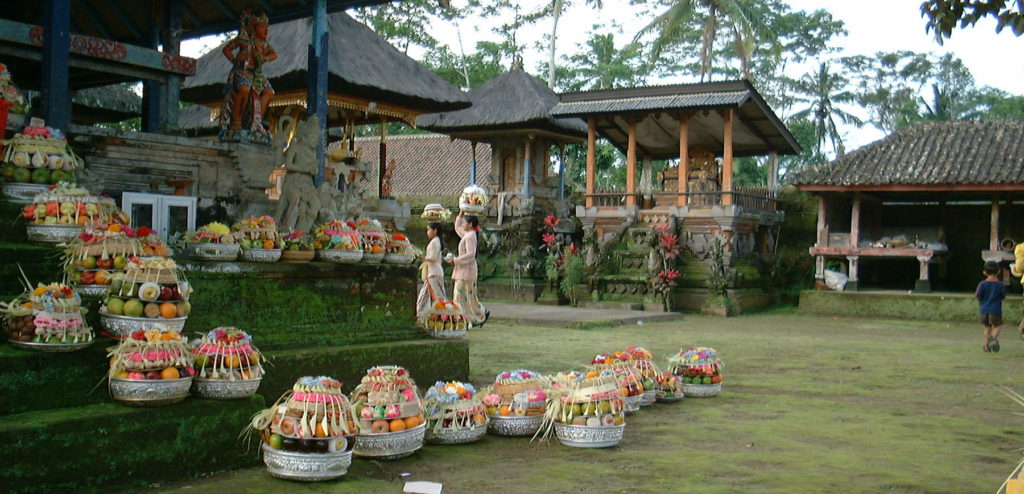
\includegraphics[width=\linewidth]{static/bali-offerings}
% % %     \caption{Canang sari}
% % %     \label{}
% % %     \end{subfigure}
% % %     \begin{subfigure}[b]{0.3\textwidth}
% % %     \centering
% % %     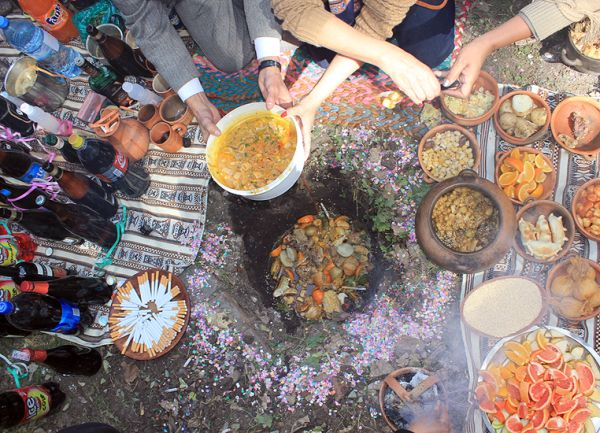
\includegraphics[width=\linewidth]{static/pachamama}
% % %     \caption{Pachamama}
% % %     \label{}
% % %     \end{subfigure}
% % %     \caption{Tecnologías de reciprocidad socio-ecológicas.}
% % %     \label{fig:mito}
% % % \end{figure}
% % % Estas cosmovisiones basadas en lógicas paraconsistentes obliga al ser humano a fomentar la coexistencia con otras formas de vida, como con otras culturas.
% % % 
% % % % Parrafo
% % % 
% % % 
% % % 
% % % 
% % % Las tecnologías de reciprocidad social y ecológica 
% % % 
% % % 
% % % 
% % % social son fundamentales para la supervivencia de las comunidades en el tiempo, pues ellas reducen las fluctuaciones individuales que ponen en peligro su estabilidad.
% % % %
% % % La teoría de la probabilidad nace en 1648 justamente como respuesta a la pregunta de cuál es el \emph{precio justo} en contextos de incertidumbre.
% % % %
% % % El problema analizaban Pascal y Fermat en sus cartas es equivalente al siguiente.
% % % %
% % % Tiramos dos veces la moneda.
% % % %
% % % Si sale seca $S$ en la primera y en la segunda, una persona (en rojo) le hace un favor a la otra.
% % % %
% % % En caso contrario, el favor se invierte.
% % % %
% % % ¿Cuál es el valor justo de la reciprocidad en este contexto de incertidumbre?
% % % 
% % % \begin{figure}[ht!]
% % %     \centering
% % %     \tikz{
% % %     \node[latent, draw=white, yshift=0.7cm, minimum size=0.1cm] (b0) {};
% % %     \node[latent,below=of b0,yshift=0.7cm, xshift=-1cm] (r1) {$S$};
% % %     \node[latent,below=of b0,yshift=0.7cm, xshift=1cm] (r2) {$C$};
% % % 
% % %     \node[latent, below=of r1, draw=white, yshift=0.8cm, minimum size=0.1cm] (bc11) {};
% % %     \node[accion, below=of r2, draw=white, yshift=0cm, color=blue!70] (bc12) {};
% % %     \node[latent,below=of bc11,yshift=0.8cm, xshift=-0.5cm] (r1d2) {$S$};
% % %     \node[latent,below=of bc11,yshift=0.8cm, xshift=0.5cm] (r1d3) {$C$};
% % % 
% % %     \node[accion,below=of r1d2,yshift=0cm, color=red!70] (br1d2) {};
% % %     \node[accion,below=of r1d3,yshift=0cm, color=blue!70] (br1d3) {};
% % %     \edge[-] {b0} {r1,r2};
% % %     \edge[-] {r1} {bc11};
% % %     \edge[-] {r2} {bc12};
% % %     \edge[-] {bc11} {r1d2,r1d3};
% % %     \edge[-] {r1d2} {br1d2};
% % %     \edge[-] {r1d3} {br1d3};
% % %     }
% % %     \caption{El problema del \emph{valor justo} que da inicio a la teoría de la probabilidad}
% % %     \label{fig:pascal-fermat}
% % % \end{figure}
% % % 
% % % La respuesta a la que arribaron Pascal y Fermat es que el valor de los favores tiene que ser inversamente proporcional a la probabilidad de hacer el favor.
% % % %
% % % Si la moneda es no sesgada, hay 1/4 de probabilidad de que salgan dos secas (terminal roja), 1/4 de que salga seca en la primera y cara en la segunda (terminal azul) y 1/2 de que salga cara en la primera (terminal azul).
% % % %
% % % Luego, la probabilidad de que la persona azul haga un favor es 3/4.
% % % %
% % % Si la persona roja hace favores por un valor equivalente a 4, el azul tiene que devolver los favores con un valor de 4/3, una relación de 3 a 1.
% % % %
% % % Esta forma intuitiva de calcular la probabilidad de un conjunto de eventos mutuamente excluyentes, como suma de sus probabilidades elementales, constituye el axioma fundamental de Kolmogorov a partir del cual se puede montar toda la teoría de la probabilidad.
% % % 
% % % % Parrafo
% % % 
% % % % 
% % % 
% % % % Parrafo
% % 
% % 
% % 
% % % Parrafo


% Kelly considera un escenario en el que una casa de apuestas ofrece pagos $Q_c$ y $Q_s$ por Cara y Seca: por cada unidad apostada la casa devuelve $Q$ si ocurre el evento apostado y $0$ en caso contrario.
% %
% La pregunta que él se hace es: ¿Cuál es la mejor forma de apostar?
% 
% % Parrafo
% 
% Supongamos que se conoce la frecuencia típica $p$ de Cara, y $1-p$ de Seca de una moneda.
% %
% El juego propuesto por Kelly entre la casa de apuestas y les apostadores sigue las reglas típicas de la vida real.
% %
% Toda persona comienza con una riqueza $\omega_0$.
% % %
% En cada ronda, la persona apuesta una proporción $b_c$ a Cara y $b_s$ a Seca.
% 
% % Parrafo
% 
% Hay dos formas de apostar.
% %
% La primera es apostar a una única de las dos opciones, por ejemplo a Caras.
% %
% En este escenario, la persona asigna un valor $ 1 \geq b_c = l > 0 $ a Caras y $b_s = 0$ a secas.
% %
% Supongamos que en la primera sale Cara y en la segunda Seca.
% %
% La riqueza en la primera es el ahorro $1-l$ más el pago que obtiene por lo apostado en Cara $l \, Q_c$.
% %
% Y en la segunda vuelta, cuando sale Seca, la riqueza es solo el ahorro, lo no apostado a Cara $1-l$.
% %
% \begin{equation}
% \omega_T = \underbrace{\overbrace{(\omega_0 \, (1-l) + \omega_0 \, l \, Q_c )}^{\omega_1} \, (1-l)}_{\omega_2} \,\dots
% \end{equation}
% %
% Lo que podemos reescribir como,
% %
% \begin{equation}
% \begin{split}
% \omega_T &= \omega_0 \, ((1-l) + \, l \, Q_c ) \, (1-l) \, \dots \\
%  &= \omega_0 \, ( (1-l) + \, l \, Q_c )^{n_c} \, (1-l)^{n_s} 
% \end{split}
% \end{equation}
% %
% donde $n_c + n_s = T$ son la cantidad de veces que salió Cara y Seca en los $T$ pasos.
% %
% Es decir, la riqueza se actualiza siguiendo un proceso multiplicativo.
% 
% % Parrafo
% 
% La otra forma de apostar consiste en utilizar todos los recursos en cada vuelta, poniendo $b_c = b$ en Cara y el resto en Seca $b_s = (1-b)$.
% %
% En este caso la riqueza se actualiza como,
% %
% \begin{equation} \label{eq:kelly_paraconsistente}
% \omega_T = \underbrace{\overbrace{(\omega_0 \, b \, Q_c)}^{\omega_1} \,  (1-b) \, Q_s}_{\omega_2} \dots = \omega_0 (b \, Q_c)^{n_c} ((1-b) \, Q_s )^{n_s}
% \end{equation}
% %
% No sólo las dos formas de apostar actualizan los recursos a través de un proceso multiplicativo. 
% %
% No es difícil demostrar que siempre existe una equivalencia.
% %
% Por ello, de aquí en adelante analizaremos únicamente esta última forma de apuestar, la que utiliza todos los recursos en cada vuelta.
% 
% % Parrafo
% 
% ¿Cuáles son los pagos que puede ofrecer una casa de apuestas?
% %
% Supongamos que la casa de apuestas ofrece pagos basados en el principio de reciprocidad analizados por Pascal y Fermat (figura \ref{fig:pascal-fermat}).
% %
% Según este principio, la pago justa debe ser inversamente proporcional a la probabilidad.
% %
% Por ejemplo, si la probabilidad de Seca es $(1-p) = 1/4$, y apostamos una unidad a Seca en cada vuelta, $3$ de cada $4$ veces vamos a perder y solo una vamos a ganar.
% %
% Luego, para que el intercambio sea ``justo'' (nadie gane), la casa de apuestas tiene que multiplicar por $Q_s = 4$ el valor apostado a Secas.
% %
% Lo mismo ocurre en Caras, $Q_c = 1/p$.
% 
% % Parrafo
% 
% En general, la casa de apuesta puede ofrecer cualquier tipo de pago.
% %
% Por ejemplo, pagos justos pero sesgados, basados en una probabilidad $q$ distinta de $p$, $Q_c = 1/q$ y $Q_s = 1/(1-q)$.
% %
% O incluso ofrecer pagos sesgados, basados en $q$, y no recíprocos que incluyen una comisión $c$, $Q_c = (1/q)\,(q\,c)$, $Q_c = (1/(1-q))\,((1-q)\,c)$.
% %
% Cuando $c = 1$, la comisión es total y tanto en Cara como en Seca la casa de apuestas simplemente devuelve los recursos apostados en la opción ganadora, $Q_c = Q_s = 1$.
% %
% Si bien en este caso no habría ningún incentivo para apostar, es interesante en tanto será (a partir del principio de coherencia que veremos en la siguiente sección) la forma natural de evaluar las hipótesis. 
% 
% % Parrafo
% 
% La tasa de crecimiento individal para cualquier tipo de pago tal que $Q_c > 0$ y $Q_s > 0$ es
% %
% \begin{equation}
% \begin{split}
% \lim_{T \rightarrow \infty } (\omega_0 \, r)^T &= \omega_0 (b \, Q_c)^{n_c} ((1-b) \, Q_s )^{n_s} \\
% r &= \lim_{T \rightarrow \infty } (b \, Q_c)^{\frac{n_c}{T}} ((1-b) \, Q_s )^{\frac{n_s}{T}} = (b \, Q_c)^{p} ((1-b) \, Q_s )^{1-p}
% \end{split}
% \end{equation}
% %
% Para maximizar $r$ tomamos el logaritmo de ambos lados, y buscamos el punto crítico de esta función cóncava,
% %
% \begin{equation}
% \begin{split}
% 0 &= \frac{d}{db} p \log (b \, Q_c) + (1-p) \log ((1-b) \, Q_s) \\
% 0 &= \frac{p}{b} + \frac{1-p}{1-b} \\
% p &= b 
% \end{split}
% \end{equation}
% %
% Sin importar el pago que elija la casa de apuestas, individualmente la tasa de crecimiento siempre se maximiza dividiendo los recursos en la misma proproción que la frecuencia típica $p$.
% %
% Pero no sólo pasa esto con el máximo, la derivada de la función tampoco depende de los pagos que ofrezca la casa de apuestas.
% %
% Este resultado Kelly lo escribe con un signo de admiración.
% %
% \begin{quotation}
% That is, \emph{the gambler ignores the posted odds} in placing his bets!
% \end{quotation}
% 
% % Parrafo
% 
% En este proceso antagónico ambos agentes pueden descubrir la verdadera probabilidad a partir de la ignoracia mutua, sin necesidad de que nadie conozca la probabilidad real.
% %
% A través de los resultados obtenidos en un juegos de apuestas podemos realizar ``inferencia''.
% % 
% El uso de las funciones de costo definidas de forma para resolver problemas de aprendizaje estadísitico es una práctica común.
% %
% El problema general del enfoque basado en funciones de costo ad-hoc tiene que ver con la influencia no deseada que decisiones arbitrarias tienen sobre las distribución de los recursos entre las hipótesis y por lo tanto sobre el resultado final de la inferencia.
% 
% % Parrafo
% 
% En este sentido, los procesos multiplicativos pueden ser vistos como la función de costo universal.
% %
% A diferencia del resto de las funciones de costo, los procesos multiplicativos tienen la propiedad especial de producir, no solo una distribución de recursos independiente de los pagos arbitrarios elegidos por la casa de apuestas (o les investigadores), sino que garantiza que en tiempo infinito la hipótesis que dividió los recursos en la misma proporción que la frecuencia típica se habrá quedado con todos los recursos que tenían las otras hipótesis.
% %
% Esto es interesante en tanto será todas las axiomatizaciones alternativas de la teoría de la probabilidad llegan a la conclusión de que la forma natural de evaluar las hipótesis es a través de un proceso multiplicativo, la ``regla del producto''.
% 
% % Parrafo
% 
% En la sección anterior analizamos las consecuencias de algunos sistemas multiplicativos.
% %
% Individualmente encontramos una ventaja a favor de lo que llamamos estrategias ``equilibradas'', que dividen los recursos en la misma proporción que la frecuencia $p$ (verificado nuevamente en esta sección).
% %
% Pero además observamos una ventaja a favor de los comportamientos cooperativos: una grupo de agentes, reduciendo las fluctuaciones individuales a través de un fondo común, logran aumentar la tasas de crecimiento hasta alcanzar, en grupos grandes, tasas equivalente al promedio aritmético de los pagos que siempre es mayor que el óptimo individual.
% %
% Pero además, una vez que surge la cooperación, el grupo de agentes puede obtener una tasa de crecimiento aún mayor a través de la especialización, asignando más recursos que al estado más frecuente de lo que conviene según la frecuencia típica $p$. 
% 
% % Parrafo
% 
% La capacidad de aumentar la tasa de crecimiento a través de la cooperación y la especialización no fue analizada por Kelly, lo que abre las siguientes preguntas.
% %
% ¿Existe un conjunto de pagos $Q_c$ y $Q_s$ que garantice la coexistencia en el tiempo entre la casa de apuestas y una población de apostadoras, o siempre se puede hacer quebrar a la casa de apuestas a través de la cooperación y la especialización?
% 
% % Parrafo
% 
% Para analizar las apuestas óptimas en grupos coopertaivos debemos analizar el comportamiento del fondo común del cual dependen sus miembros.
% %
% En cada ronda, una cantidad $n_c$ de miembros van a recibir Caras y una cantidad $n_s$ va a recibir Secas.
% %
% El fondo común en un tiempo $t+1$ es la suma de todos los recursos individuales en el tiempo $t$.
% %
% Cuando el tamaño del grupo tiende a infinito, la cuota que se recibe del fondo común $\omega_{t+1}$ es equivalente al promedio de los estados.
% %
% \begin{equation}
% \begin{split}
% \lim_{N \rightarrow \infty} N \omega_{t+1} &= (\omega_t \, b \, Q_c ) \, n_c + (\omega_t \, (1-b) \, Q_s ) \, n_s \\
%  \omega_{t+1} &=  \omega_t \, \underbrace{\left(  b \, Q_c \, p +  (1-b) \, Q_s \, (1-p) \right)}_{\text{Tasa de crecimiento } r} 
% \end{split}
% \end{equation}
% %
% Si el pago es recíproco, $Q_c = 1/p$ y $Q_s = 1/(1-p)$, la tasa de crecimiento de la cuota del fondo común siempre vale $1$, más allá de la apuesta $b$ que elija el grupo coopertaivo!
% \begin{equation}
% \begin{split}
% r &=  b \, \frac{1}{p} \, p +  (1-b) \, \frac{1}{1-p} \, (1-p) = b + (1 - b) = 1
% \end{split}
% \end{equation}
% %
% Cooperar tiene una ventaja respecto de jugar individualmente, no importa si la apuesta es incorrecta, los individuos del grupo cooperativo nunca pierden.
% 
% % Parrafo
% 
% Los pago recíprocos garantizan entonces la coexistencia de una casa de apuestas con un grupo cooperativo.
% %
% Todo otro pago que ofrezca la casa de apuestas puede ser aprovechado por el grupo cooperativo.
% %
% Y a través de la especialización podrán obtener una tasa de crecimiento mayor que los agentes individuales, como vimos en la sección anterior.
% %
% Si bien la cooperación es útil para reducir fluctuaciones y aumentar la tasa de crecimiento en un juego de apuestas, jugar de forma cooperativa elimina la propiedad fundamental que hace de los procesos multiplicativos un función de costo útil como mecanismo de inferencia: la apuesta óptima ya no será aquella que divide los recursos en la misma proporción que la frecuencia típica.


















































































































\chapter{Probabilidad (Bayesiana): las verdades empíricas.} \label{ch:proba}

\epigraph{El conocimiento empírico no es más que principio de indiferencia compatible con la evidencia formal y empírica}{}

La ciencia es una institución humana que tiene pretención de verdad.
%
Las ciencias formales validan sus proposiciones mediante teoremas, resultados derivados de aplicar las reglas internas a un sistema axiomático cerrado.
%
Las ciencias empíricas, por el contrario, deben validar sus proposiciones dentro de sistemas abiertos, lo que impone siempre un grado de incertidumbre asociada.
%
¿Cuál es entonces la fuente de validez del conocimiento empírico, y por qué?

% Parrafo

La coexistencia como fuente de validez del conocimiento nos obliga a rechazar la superiordad moral de subjetividades especiales o identidades particulares (criterio de autoridad) y a trabajar activamente para construir acuerdos intersubjetivos que garanticen el principio de reconocimiento mutuo (criterio de universalidad).
%y no como la imposición automática del objeto al sujeto (objetividad),.
%
Elegimos el término ``intersubjetividad'', por sobre el de ``subjetividad'', debido a que el primero connota el cumplimiento de condiciones que son necesarias para producir el acuerdo entre las conciencias individuales, mientras que el segundo connota una arbitrariedad que lo obstaculiza.
%
Elegimos el término ``intersubjetividad'', por sobre el de ``objetividad'', porque el primero connota una actividad constructiva entre los sujetos, mientras que el segundo connota la imposición directa del objeto sobre los sujetos.

% Parrafo

Para el proyecto intercultural de acuerdos intersubjetivos, que se propone la ciencia, se hace necesario que los individuos pongan en correspondencia unívoca los fenómenos percibidos por sus conciencias con algún esquema de operación que sea públicamente inteligible y reproducible.
% 
En este sentido, las funciones ocupan un rol fundamental.
%
En su definición formal, una función es una relación (u operación) $f$ que a cada elemento de un conjunto (dominio) $X$ asigna un único elemento de otro conjunto (imagen) $Y$.
%
\begin{equation}
 \forall x \in X \  \exists! y \in Y \text{ tal que } f(x) = y    
\end{equation}
%
%A primera vista puede parecer que las funciones no tienen nada en especial respecto de otro tipo de relaciones posibles entre conjuntos.
Lo que hace tan poderosa a las funciones como herramienta para la ciencia es el hecho de que ellas permiten definir asignaciones no ambiguas.

% Parrafo

Los funciones son la base de las ciencias formales.
%
Todos los sistemas matemáticos de interés están compuestos por axiomas $X$, una serie de operaciones válidas $F$, y un conjunto de consecuencias $Y$ consistentes entre sí.
%
En teoría de la computabilidad, la tesis de Church-Turing afirma que toda función sobre los números naturales puede ser calculada por un ``método efectivo'' si y sólo si es computable por una máquina de Turing.
%
Debido a que todos las definiciones alternativas del concepto  de ``método efectivo'' resultaron ser equivalentes a una maquina de Turing, actualmente se supone que la hipótesis Church-Turing es cierta.

% Parrafo

Las funciones son también la base de las ciencias empíricas.
%
Veremos cómo los tres conceptos fundamentales de toda teoría empírica, los modelos causales, los datos y la incertidumbre tienen una estructura funcional.
%
En la sección \ref{sec:principios_interculturales} introduciremos los principios interculturales de acuerdos intersubjetivos
que garantizan los acuerdos intersubjetivos en contextos de incertidumbre.
%
En la sección \ref{sec:reglas_de_la_probabilidad} presentaremos las reglas que se derivan del sistema de acuerdos intersubjetivos y explicaremos por qué garantiza la adquisición de conocimiento empírico.
%
Uno de los principales problemas a resolver en ciencias empíricas es la aparición de modelos causales alternativos que compiten por la explicación de un mismo conjunto de observables.
%
En la sección \ref{sec:modelos_alternativos} mostramos cómo las reglas de este sistema permiten realizar una selección intersubjetiva de modelos causales alternativos.
%
El otro problema fundamental en ciencias empíricas es la constucción de nuevos datos que sirvan como base empírica para evaluar nuevas hipótesis.
%
En la sección \ref{sec:base_empirica_metodo} dónde se ubican las hipótesis dentro de la estructura invariante del dato científico, y cómo el sistema de acuerdos intersubjetivos garantiza la construcción nueva base empírica para la actividad científica normal.

\section{Principios interculturales de acuerdos intersubjetivos}\label{sec:principios_interculturales}

Las verdades empíricas requieren que alcancemos acuerdos intersubjetivos, universales, en contextos de incertidumbre.
%
Un sistema lógico con esas propiedades puede derivarse de principios filosóficos con validez intercultural.
%
En primer lugar, ``el principio de razón suficiente'' es la base para el desarrollo de modelos causales.
%
El ``principio de indiferencia'' garantiza un primer acuerdo intersubjetivo en contextos de incertidumbre, maximizando la diversidad de creencias mutuamente contradictorias del modelo causal.
%
Luego, el ``principio de coherencia'' garantiza la continuidad del acuerdo intersubjetivo mediante la preservación de la creencia que que sigue siendo compatible con los datos de base empírica.
%
Finalmente, el ``principio de integridad'' garantiza que no exista ni pérdida ni creación espontanea de creencias.

\subsection{Principio de razón suficiente}

La idea de que todo lo que ocurre en la naturaleza debe tener una causa previa que lo genere se conoce en la historia de la filosofía como el principio de \emph{razón suficiente}.
%
En pocas palabras, todo tiene una explicación suficiente.
%Leibniz (1646-1716),  \cite{Leibniz and China: A Commerce of Light}
%La Monadología (escrita en francés en 1714 y publicada en alemán en 1720) es una de las obras de Gottfried Leibniz que mejor resume su filosofía. Escrita hacia el final de su vida para sustentar una metafísica de las sustancias simples, es un tratado acerca de las mónadas, que son los átomos verdaderos, es decir, realmente indivisibles. Se puede decir que es una proposición filosófica o metafísica, aunque en ambos casos viene a significar lo mismo \cite{leibniz1714-monadologie}.
%
Este principio es la base del concepto de causa y efecto, que tiene nuevamete una estructura funcional, $f(x) = y$, donde $x$ representa las condiciones iniciales, $f$ el modelo causal determinista, e $y$ el efecto.

% Parrafo

El fundador de la inferencia Bayesiana moderna, Pierre-Simon Laplace (1749-1827), tenía la convicción de que si tuvieramos conocimiento completo (infinitamente preciso) del estado del mundo $x$ en un instante de tiempo, y el modelo causal correcto que rige el comportamiento del mundo $f$, entonces tendríamos conocimiento completo del estado del mundo en cualquier instante posterior $y$.
%
Aunque esta afirmación sea cierta, la historia de la ciencia reciente a mostrado que conocer el mundo con precisión \emph{finita} es suficiente parra introducir una incertidumbre que impide predecir el comportamiento de modelos causales incluso en el corto plazo.

% Parrafo

Un ejemplo de sistema determinista capaz de adquirir comportamientos imprevisibles es el siguiente modelo ``poblacional''.
%
\begin{equation}
 \text{Población}(t+1) = r \cdot \text{Población}(t)\cdot (1-\text{Población}(t))
\end{equation}
%
El modelo establece que el tamaño de una población, medida como proporción respecto de la capacidad máxima de un sistema, depende exclusivamente de su tamaño en el tiempo anterior y de un factor de reproducción $r$.
%
Las relaciones causales se suelen expresar en términos gráficos.

% Parrafo

\begin{figure}[ht!]
\centering
\tikz{         
    \node[latent, minimum size=1.25cm] (n1) {$\text{pob}_n$} ; 
    
    \node[latent, right=of n1, xshift=3cm, minimum size=1.25cm] (n2) {$\text{pob}_{n+1}$} ;
    
     \path[->] (n1) edge node [yshift=0.5cm] {$r \cdot \text{pob}_n \cdot (1-\text{pob}_n)$} (n2);

}
\caption{Modelo causal expresado gráficamente. Las flechas representan la relación causal entre las variables. }
\label{fig:modelo_poblacional}
\end{figure}

% Parrafo

Dependiendo del factor de reproducción $r$ y de la población inicial pop$_0$, vemos diferentes tipos de comportamiento.
%
Por ejemplo, dada una población incial $\text{pop}_0 = 0.5$, cuando el valor del parámetro $r$ es bajo (figura~\ref{fig:poblacion_punto_fijo}) la población tiende a un valor fijo;
cuando es intermedio (figura~\ref{fig:poblacion_periodico}) la población oscila en un período;
y cuando llega a su límite máximo (figura~\ref{fig:poblacion_caotico}) la población tiene un comportamiento denominado ``caótico''.
%
\begin{figure}[ht!]
    \centering
    \begin{subfigure}[b]{0.32\textwidth}
    \includegraphics[page=3,width=\linewidth]{figures/poblacion.pdf}
    \caption{Punto fijo}
    \label{fig:poblacion_punto_fijo}
    \end{subfigure}
    \begin{subfigure}[b]{0.32\textwidth}
    \includegraphics[page=9,width=\linewidth]{figures/poblacion.pdf}
    \caption{Periódico}
    \label{fig:poblacion_periodico}
    \end{subfigure}
    \begin{subfigure}[b]{0.32\textwidth}
    \includegraphics[page=11,width=\linewidth]{figures/poblacion.pdf}
    \caption{Caótico}
    \label{fig:poblacion_caotico}
    \end{subfigure}
    \caption{
    Tipos de atractores del modelo causal no-lineal
    }
    \label{fig:poblacion}
\end{figure}
%
Bajo un régimen caótico no se observan períodos de ninguna longitud, el sistema produce trayectorias que nunca pasan por los mismos puntos.
%
En la figura \ref{fig:pseudo_aleatorio} vemos que los primeros 2000 puntos de la trayectoria determinista que comienza con $r=3.99$ y $\text{pop}_0 = 0.5$ se parece a una variable aleatoria.

% Parrafo

Otra de las propiedades del atractor caótico es la sensibilidad a las condiciones inciales.
%
En la figura~\ref{fig:poblacion_caotico} hacemos zoom en los primeros 30 pasos temporales y observamos que si modificamos levemente las condiciones iniciales las trayectoria rápidamente divergen hasta volverse completamente diferentes.

%

\begin{figure}[ht!]
    \centering
    \begin{subfigure}[b]{0.4\textwidth}
    \centering
    \includegraphics[page=14,width=\linewidth]{figures/poblacion}
    \caption{Comportamiento que parece aleatorio}
    \label{fig:pseudo_aleatorio}
    \end{subfigure}
    \begin{subfigure}[b]{0.4\textwidth}
    \centering
    \includegraphics[page=13,width=\linewidth]{figures/poblacion}
    \caption{Sensibilidad a condiciones iniciales}
    \label{fig:sensibilidad}
    \end{subfigure}
    \caption{Comportamiento del modelo causal no lineal con $r=3.99$ y $\text{pop}_0 = 0.5$.
    (\subref{fig:pseudo_aleatorio}): primeros 2000 puntos.
    (\subref{fig:sensibilidad}): primeros 30 puntos. La linea roja comienza con $\text{pop}_0 = 0.499$.}
    \label{fig:propiedades_caoticas}
\end{figure}

%

La sensibilidad a las condiciones iniciales impone un límite a la capacidad predicitiva.
%
Por más que la natrualeza sea determinista y conozcamos el mecanismo subyacente, si el sistema se encuentra en atractor caótico, jamás vamos a poder predecir el destino inevitable más allá de cierto tiempo debido a que en ningún sistema natural podremos medir con infinita precisión las condiciones inciales.
%
La imposibilidad de determinar si estamos en presencia de las ``mismas condiciones iniciales'' es una fuente de incertidumbre que tiene toda ciencia empírica.

\subsection{Principio de integridad}\label{sec:principio_integridad}

Las verdades empíricas siempre contienen incertidumbre.
%
Hemos visto que un posible origen puede ser la sensibilidad a las condiciones inciales de una naturaleza puramente causal.
%
Sin embargo, desde las ciencias sociales y la física cuántica se suele afirmar que el mundo no tiene forma de función: que incluso conociendo las condiciones inciales con precisión infinita no existe una función que permita determinar el estado del mundo en un tiempo posterior.

% Parrafo

El concepto de libre albedrío de las ciencias sociales afirma que una persona expuesta ante un estado del universo determinado, bajo exactamente las mismas condiciones iniciales, tiene todavía la capacidad de elegir una acción.
%
Ya no es posible definir una función tal que dado el estados inical del universo $s$ devuelva la acción $a$ que tomará el sujeto, $f(s) = a$.
%
Sea porque el mundo natural admite la posibilidad de que un efecto surga sin su propia causa, sea por nuestra incapacidad de conocer los modelos causales correctos o de conocer las condiciones iniciales con infinita precisión, nuestro conocimiento sobre el mundo natural contiene siempre un grado de incertidumbre.

% Parrafo

Supongamos que sabemos que las acciones sobre las que puede eligr la persona se limitan a esconder un regalo detrás de una caja de tres.
%
Se abren así tres ``universos paralelos'' posibles, uno por cada una de las acciones (figura~\ref{fig:libre_albedrio}).
%
\begin{figure}[ht!]
\centering
\begin{subfigure}[b]{0.48\textwidth}
\centering
    \scalebox{1}{
 \tikz{ %
        \node[estado] (s) {};
        \node[const, above=of s] {$s$};
        \node[accion, below=of s, xshift=-1cm] (a1) {} ; %
	\node[accion, below=of s, xshift=0cm] (a2) {} ; %
	\node[accion, below=of s, xshift=1cm] (a3) {} ; %
	\node[const, right=of a3] {$a$};
        \edge[-] {s} {a1,a2,a3};
      
	\node[estado, below=of a1,xshift=0cm] (s1a) {}; %
	  
	\node[estado, below=of a2,xshift=0cm] (s2a) {}; %
	   
	\node[estado, below=of a3,xshift=0cm] (s3a) {}; %
	    
	\node[const, right=of s3a] {$s^{\prime}$};
	\edge[-] {a1} {s1a};
	\edge[-] {a2} {s2a};
	\edge[-] {a3} {s3a};
        }
    
    }
    \caption{Libre albedrío}
    \label{fig:libre_albedrio}
\end{subfigure}
\begin{subfigure}[b]{0.48\textwidth}
 \centering
 \tikz{
    \node[factor, minimum size=0.8cm] (p1) {} ;
    \node[factor, minimum size=0.8cm, xshift=1.5cm] (p2) {} ;
    \node[factor, minimum size=0.8cm, xshift=3cm] (p3) {} ;
    
    \node[const, above=of p1, yshift=.15cm] (fp1) {$P(a_1)$};
    \node[const, above=of p2, yshift=.15cm] (fp2) {$P(a_2)$};
    \node[const, above=of p3, yshift=.15cm] (fp3) {$P(a_1)$};
    } 
   \caption{Espacio de hipótesis}
   \label{fig:espacio_de_hipotesis}
\end{subfigure}
    \caption{(a) El concepto teórico libre albedrío afirma que una persona, ante un estados $s$ del universo, es capaz de elegir entre más de una acción $a_i$.
    (b) Espacio de hipótesis: sabemos que hay un regalo detrás de sólo una de las tres cajas. }
\end{figure}
%
Cuando la incertidumbre nos impide conocer la función que gobierna el mundo, podemos todavía expresar nuestra incertidumbre utilizando funciones de probabilidad, que para cada hipótesis $a$ asigne una proporción $p$ de nuestra creencia total, $P(a_i) = p_i$.
%
En este caso, la acción de esconder el regalo detrás de una de las tres cajas representan nuestro \emph{espacio de hipótesis} (figura~\ref{fig:espacio_de_hipotesis}).
%
Y las diferentes formas de dividir la creencia le vamos a llamar \emph{distribución de creencias}.

% Parrafo

El ``principio de integridad'' establece la conservación de la creencia total, garantizando que no haya perdidas ni generación espontánea de creencias.
%
Esto es, que la suma de las proporiciones asignadas a cada una de las hipótesis es $1$.
%
\begin{equation}
\sum_{i} P(\text{hipótesis}_i) = 1
\end{equation}
%
Bajo este principio hay infinitas distribuciones de creencias posibles.
%
Por ejemplo, podemos tener el presentimiento de que está en la caja del medio.
%
En la figura \ref{fig:distribucion_de_creencias} mostramos dos posibles distribuciones de creencias que tienen preferencia esa caja.
%
La distribución de creencias de la figura~\ref{fig:preferencia_total} representa la certeza de que el regalo está en la caja del medio, mientras que la figura~\ref{fig:preferencia_parcial} representa una preferencia parcial que mantiene todavía cierta duda.

% PArrafo

\begin{figure}[ht!]     
 \centering
 \begin{subfigure}[b]{0.48\textwidth}
 \centering
  \tikz{ %
         \node[factor, minimum size=0.8cm] (p1) {} ;
         \node[factor, minimum size=0.8cm, xshift=1.5cm] (p2) {} ;
         \node[factor, minimum size=0.8cm, xshift=3cm] (p3) {} ;
         
         \node[const, above=of p1, yshift=.15cm] (fp1) {$0$};
         \node[const, above=of p2, yshift=.15cm] (fp2) {$1$};
         \node[const, above=of p3, yshift=.15cm] (fp3) {$0$};        
        }
    \caption{Preferencia total}
    \label{fig:preferencia_total}
 \end{subfigure}
 \begin{subfigure}[b]{0.48\textwidth}
 \centering
  \tikz{ %
         \node[factor, minimum size=0.8cm] (p1) {} ;
         \node[factor, minimum size=0.8cm, xshift=1.5cm] (p2) {} ;
         \node[factor, minimum size=0.8cm, xshift=3cm] (p3) {} ;
         
         \node[const, above=of p1, yshift=.15cm] (fp1) {$1/10$};
         \node[const, above=of p2, yshift=.15cm] (fp2) {$8/10$};
         \node[const, above=of p3, yshift=.15cm] (fp3) {$1/10$};        
        } 
    \caption{Preferencia parcial}
    \label{fig:preferencia_parcial}
 \end{subfigure}
\caption{Dos distribución de creencias que tienen preferencia por una de las hipótesis.}
 \label{fig:distribucion_de_creencias}
\end{figure}

% Parrafo

¿Pero cuál de todas las infinitas posibles distribuciones de creencias tiene validez intersubjetiva?

\subsection{Principio de indiferencia}\label{sec:principio_indiferencia}

El ``principio de indiferencia'' es un principio de validez intercultural que permite llegar a un primer acuerdo intersubjetivo en contextos de incertidumbre.
%
En los casos donde sólo conocemos el espacio de hipótesis y no tenemos más información que nos permita tener preferencia por ninguna de las opciones, vamos a estar de acuerdo en la necesidad de dividir la creencia en partes iguales por los caminos parallelos del modelo causal.
%
\begin{figure}[ht!]
\begin{subfigure}[b]{0.2\textwidth}
  \centering \vskip 0pt
  \tikz{            
    \node[latent] (r) {
\includegraphics[width=0.24\textwidth]{static/regalo.png}} ;
    \node[const,above=of r, yshift=.15cm] (nr) {$r \in \{1,2,3\}$} ; 
    \node[const, below=of r, yshift=-0.8cm] (title) {(a) Modelo causal};
   }
   
\end{subfigure}
\begin{subfigure}[b]{0.44\textwidth}
    \centering \vskip 0pt
    \tikz{
    \node[latent, draw=white, yshift=0.6cm] (b0) {$1$};
       
    \node[latent,below=of b0,yshift=0.6cm, xshift=-1.6cm] (r1) {$r_1$};
    \node[latent,below=of b0,yshift=0.6cm] (r2) {$r_2$};
    \node[latent,below=of b0,yshift=0.6cm, xshift=1.6cm] (r3) {$r_3$};

    \node[latent, below=of r1, draw=white, yshift=0.6cm] (br1) {$\frac{1}{3}$};
    \node[latent, below=of r2, draw=white, yshift=0.6cm] (br2) {$\frac{1}{3}$};
    \node[latent, below=of r3, draw=white, yshift=0.6cm] (br3) {$\frac{1}{3}$};
    \edge[-] {b0} {r1,r2,r3};
    \edge[-] {r1} {br1};
    \edge[-] {r2} {br2};
    \edge[-] {r3} {br3};
    
    \node[const, below=of br2, yshift=-0.1cm] (title) {(b) Caminos del modelo causal};
    }
\end{subfigure}
\begin{subfigure}[b]{0.32\textwidth}
\centering\vskip 0pt
\tikz{ %
        
         \node[factor, minimum size=1cm] (p1) {} ;
         \node[factor, minimum size=1cm, xshift=1.5cm] (p2) {} ;
         \node[factor, minimum size=1cm, xshift=3cm] (p3) {} ;
         \node[const, above=of p1, yshift=.15cm] (fp1) {$1/3$};
         \node[const, above=of p2, yshift=.15cm] (fp2) {$1/3$};
         \node[const, above=of p3, yshift=.15cm] (fp3) {$1/3$};
         \node[const, below=of p2, yshift=-0.8cm] (title) {(c) Creencia honesta};
         
        } 
\end{subfigure}
\caption{Principio de indiferencia. Figura (a): el modelo causal tiene una única variable $r$ que puede tomar tres valores posibles. Figura (b): el modelo causal induce tres caminos paralelos por los que dividimos la creenciencia en partes iguales. Figura (c): como resultado obtenemos una creencia honesta que garantiza los acuerdos intersubjetivos dado el modelo causal.
}
\label{fig:principio_de_indiferencia}
\end{figure}
%
A este tipo de distribuciones de creencias que permiten alcanzar acuerdos intersubjetivos en contextos de incertidumbre las vamos a llamar \emph{creencia honestas}.

% Parrafo

El principio de indiferencia puede generalizarse a modelos causales multidimensional.
%
Para ejemplificar, supongamos que nos permiten elegir una caja $c$ y que después alguien nos señala con certeza que el regalo no está en la caja señalada, $s$.
%
Es decir, tenemos tres variables y una dependencia causal, la psita $s$ depende de la posición del regalo $r$.
%
¿Será que nuestra elección $c$ también afecta la pista $s$, que la pista además de no señalar la caja donde está el regalo tampoco señala la caja elegida?.

% Parrafo

En este contexto podemos proponer al menos dos modelos causales multidimensionales alternativos.
%
En el primero hay sólo una dependencia causal, la pista no señala la posición del regalo, que podemos representar con el modelo causal de la figura~\ref{fig:modelo_causal_1}
%
En el segundo hay dos dependencias causales, la pista no señala ni la posición del regalo ni la caja elegida, que podemos representar con el modelo causal de la figura~\ref{fig:modelo_causal_2}.
%
Para simplificar el problema, consideraremos que la caja elegida es $c=1$.

% Parrafo

\begin{figure}[ht!]
  \centering
  \begin{subfigure}[b]{0.48\textwidth}
  \centering
  \tikz{            
    \node[latent,] (r) {
\includegraphics[width=0.12\textwidth]{static/regalo.png}} ;
    \node[const,left=of r] (nr) {\Large $r$} ;    
    
    
    \node[latent, below=of r] (d) {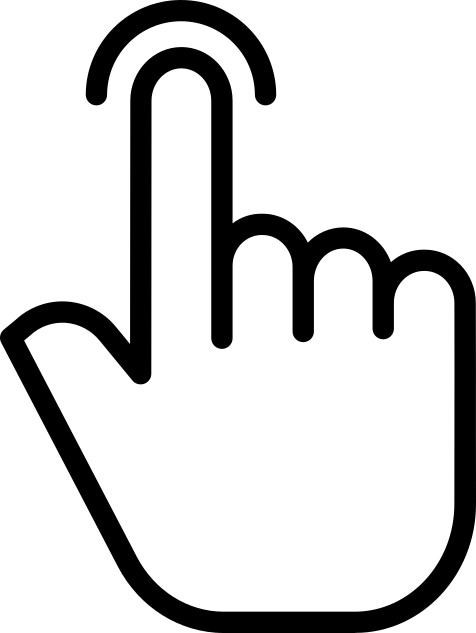
\includegraphics[width=0.10\textwidth]{static/dedo.png}} ;
    \node[const, left=of d] (nd) {\Large $s$};
    %\node[const, below=of d] (pd) {$\text{Creencia}(s=i|r=i, \text{Modelo}) = 0$}; 

    \edge {r} {d};
  }
  \caption{Modelo A}
  \label{fig:modelo_causal_1}
  \end{subfigure}
  \begin{subfigure}[b]{0.48\textwidth}
  \centering
  \tikz{        
    
    \node[latent] (d) {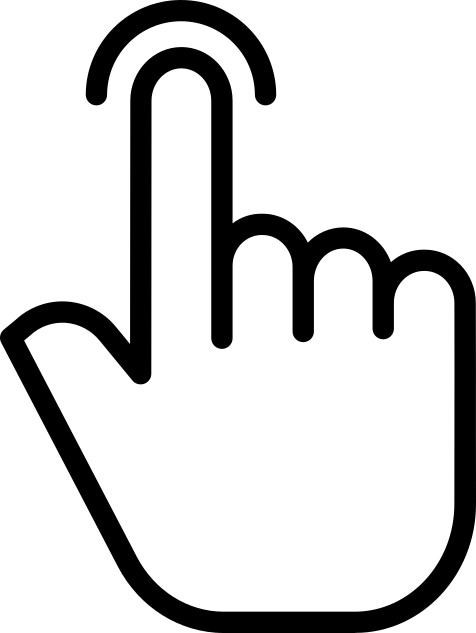
\includegraphics[width=0.10\textwidth]{static/dedo.png}} ;
    \node[const,above=of d] (nd) {\Large $s$} ;
    
    \node[latent, above=of d, xshift=-1.5cm] (r) {
\includegraphics[width=0.12\textwidth]{static/regalo.png}} ;
    \node[const,above=of r] (nr) {\Large $r$} ;
    
    \node[latent, fill=black!30, above=of d, xshift=1.5cm] (c) {
\includegraphics[width=0.12\textwidth]{static/cerradura.png}} ;
    \node[const,above=of c] (nc) {\Large $c=1$} ;
    
    \edge {r,c} {d};
  }
  \caption{Modelo B}
  \label{fig:modelo_causal_2}
  \end{subfigure}
  \caption{Modelos causales alternativos. Figura~\ref{fig:modelo_causal_1}: la pista sólo depende de la posición del regalo. Figura~\ref{fig:modelo_causal_2}: la pista depende de la posición del regalo y la la caja elegida previamente.
  Los círculos representan las variables y la felcha representa la relación causa $\rightarrow$ efecto. 
  %A su vez, $r=i$ representa la proposición ``el regalo se encuentra en la posición $i$'', y $s=i$ representa la proposición ``la pista señala la posición $i$''.
  }
  \label{fig:modelos_causales}
\end{figure}

% Parrafo
% %
% Por último, lo que aparece del lado izquierdo del operador \emph{condicional} ($\cdot \mid \cdot$) son las proposiciones sobre las que computamos la creencia en los casos en los que las proposiciones que aparecen del lado derecha sean ciertas.
% %
% Es decir, la $\text{Creencia}(s=i|r=i,\text{Modelo}) = 0$ se lee como ``es imposible que la pista señale la posición $i$ cuando el regalo está en la posición $i$ y el modelo causal es cierto''. 
% 

% % Parrafo

Cada uno de los modelos causales alternativos tiene su propio conjuto finito de universos paralelos.
%
Siguiendo con el principio de indiferencia (o de máxima diversidad) dividimos la creencia en partes iguales en cada una de las bifurcaciones de los caminos paralelos del modelo causal.
%
En la figura~\ref{fig:caminos} mostramos cómo se dividen las creencias en partes iguales por los caminos paralelos de ambos modelos causales.

% Parrafo

En el modelo A, por cada posición del regalo, se abren otros dos unviersos paralelos que se corresponden con las cajas hacia las que puede señalar la pista, en las que no está el regalo en ese universo.
%
En cambio, en el modelo B, la pista genera dos universos sólo cuando el regalo está en la misma caja que elegimos, $r=1$.
%
% Podemos recibir una pista tanto en la puerta 2, $s_2$, como en la puerta 3, $s_3$.
% %
% Cuando el regalo está en otra caja, $r\neq 1$, la pista puede señalar únicamente a una de las cajas, la que no tiene el regalo y la que no fue elegida.
% %
% Por ejemplo, si el regalo está en la puerta 2, $r_2$, la pista sólo puede señalar la puerta 3, $s_3$.
%
\begin{figure}[H]
\centering
\begin{subfigure}[b]{0.48\textwidth}
\centering
\tikz{
\node[latent, draw=white, yshift=0.7cm] (b0) {$1$};

\node[latent,below=of b0,yshift=0.7cm, xshift=-2cm] (r1) {$r_1$};
\node[latent,below=of b0,yshift=0.7cm] (r2) {$r_2$};
\node[latent,below=of b0,yshift=0.7cm, xshift=2cm] (r3) {$r_3$};

\node[latent, below=of r1, draw=white, yshift=0.7cm] (br1) {$\frac{1}{3}$};
\node[latent, below=of r2, draw=white, yshift=0.7cm] (br2) {$\frac{1}{3}$};
\node[latent, below=of r3, draw=white, yshift=0.7cm] (br3) {$\frac{1}{3}$};
\node[latent,below=of br1,yshift=0.7cm, xshift=-0.5cm] (r1d2) {$s_2$};
\node[latent,below=of br1,yshift=0.7cm, xshift=0.5cm] (r1d3) {$s_3$};

\node[latent,below=of r1d2,yshift=0.7cm,draw=white] (br1d2) {$\frac{1}{3}\frac{1}{2}$};
\node[latent,below=of r1d3,yshift=0.7cm, draw=white] (br1d3) {$\frac{1}{3}\frac{1}{2}$};
\node[latent,below=of br2,yshift=0.7cm, xshift=-0.5cm] (r2d1) {$s_1$};
\node[latent,below=of br2,yshift=0.7cm, xshift=0.5cm] (r2d3) {$s_3$};
\node[latent,below=of br3,yshift=0.7cm, xshift=-0.5cm] (r3d1) {$s_1$};
\node[latent,below=of br3,yshift=0.7cm, xshift=0.5cm] (r3d2) {$s_2$};

\node[latent,below=of r2d1,yshift=0.7cm, draw=white] (br2d1) {$\frac{1}{3}\frac{1}{2}$};
\node[latent,below=of r2d3,yshift=0.7cm,draw=white] (br2d3) {$\frac{1}{3}\frac{1}{2}$};
\node[latent,below=of r3d1,yshift=0.7cm, draw=white] (br3d1) {$\frac{1}{3}\frac{1}{2}$};
\node[latent,below=of r3d2,yshift=0.7cm,draw=white] (br3d2) {$\frac{1}{3}\frac{1}{2}$};
\edge[-] {b0} {r1,r2,r3};
\edge[-] {r1} {br1};
\edge[-] {r2} {br2};
\edge[-] {r3} {br3};
\edge[-] {br1} {r1d2,r1d3};
\edge[-] {r1d2} {br1d2};
\edge[-] {r1d3} {br1d3};
\edge[-] {br2} {r2d1, r2d3};
\edge[-] {br3} {r3d1,r3d2};
\edge[-] {r2d1} {br2d1};
\edge[-] {r2d3} {br2d3};
\edge[-] {r3d1} {br3d1};
\edge[-] {r3d2} {br3d2};
}
\caption{Modelo A}
\label{fig:caminos_pre_montyhall}
\end{subfigure}
\begin{subfigure}[b]{0.48\textwidth}
\centering
\tikz{
\node[latent, draw=white, yshift=0.7cm] (b0) {$1$};
\node[latent,below=of b0,yshift=0.7cm, xshift=-2cm] (r1) {$r_1$};
\node[latent,below=of b0,yshift=0.7cm] (r2) {$r_2$};
\node[latent,below=of b0,yshift=0.7cm, xshift=2cm] (r3) {$r_3$};

% \node[latent, below=of r1, draw=white, yshift=0.8cm] (br1) {$\frac{1}{3}$};
% \node[latent, below=of r2, draw=white, yshift=0.8cm] (br2) {$\frac{1}{3}$};
% \node[latent, below=of r3, draw=white, yshift=0.8cm] (br3) {$\frac{1}{3}$};
% \node[latent,below=of br1,yshift=0.8cm] (c11) {$c_1$};
% \node[latent,below=of br2,yshift=0.8cm] (c12) {$c_1$};
% \node[latent,below=of br3,yshift=0.8cm] (c13) {$c_1$};

\node[latent, below=of r1, draw=white, yshift=0.7cm] (bc11) {$\frac{1}{3}$};
\node[latent, below=of r2, draw=white, yshift=0.7cm] (bc12) {$\frac{1}{3}$};
\node[latent, below=of r3, draw=white, yshift=0.7cm] (bc13) {$\frac{1}{3}$};
\node[latent,below=of bc11,yshift=0.7cm, xshift=-0.5cm] (r1d2) {$s_2$};
\node[latent,below=of bc11,yshift=0.7cm, xshift=0.5cm] (r1d3) {$s_3$};
\node[latent,below=of bc12,yshift=0.7cm] (r2d3) {$s_3$};
\node[latent,below=of bc13,yshift=0.7cm] (r3d2) {$s_2$};

\node[latent,below=of r1d2,yshift=0.7cm,draw=white] (br1d2) {$\frac{1}{3}\frac{1}{2}$};
\node[latent,below=of r1d3,yshift=0.7cm, draw=white] (br1d3) {$\frac{1}{3}\frac{1}{2}$};
\node[latent,below=of r2d3,yshift=0.7cm,draw=white] (br2d3) {$\frac{1}{3}$};
\node[latent,below=of r3d2,yshift=0.7cm,draw=white] (br3d2) {$\frac{1}{3}$};
\edge[-] {b0} {r1,r2,r3};
% \edge[-] {r1} {br1};
% \edge[-] {r2} {br2};
% \edge[-] {r3} {br3};
% \edge[-] {br1} {c11};
% \edge[-] {br2} {c12};
% \edge[-] {br3} {c13};
\edge[-] {r1} {bc11};
\edge[-] {r2} {bc12};
\edge[-] {r3} {bc13};
\edge[-] {bc11} {r1d2,r1d3};
\edge[-] {bc12} {r2d3};
\edge[-] {bc13} {r3d2};
\edge[-] {r1d2} {br1d2};
\edge[-] {r1d3} {br1d3};
\edge[-] {r2d3} {br2d3};
\edge[-] {r3d2} {br3d2};
}
\caption{Modelo B}
\label{fig:caminos_montyhall}
\end{subfigure}
\caption{Los caminos paralelos que se generan a partir de los modelos causales alternativos. El principio de máxima diversidad (o de indiferencia) divide la creencia en partes en cada una de las bifurcaciones de los caminos paralelos del modelo causal. }
\label{fig:caminos}
\end{figure}
%
Esto nos permite definir creencias honestas respecto de los universos paralelos. 
%
Cada camino del modelo causal tiene una combinación de valores distinta que representa nuestra \emph{creencia conjunta} honesta de que el regalo se encuentre en la caja $i$ y la pista señale la caja $j$.
%
% Por ejemplo, la creencia conjunta de que el regalo esté en la caja $2$ y la pista señale la caja $3$ es
% \begin{equation}
% \text{Creencia}(r=2 \wedge s=3 | \text{Modelo A} ) = \frac{1}{3} \frac{1}{2} = \frac{1}{6} \ \ \ \ \ \ \text{Creencia}(r=2 \wedge s=3 | \text{Modelo B} ) = \frac{1}{3} 
% \end{equation}
% %
% Donde $\wedge$ representa el conjunción lógica.
% %
% De aquí en adelante remplazaremos este símbolo por una simple coma ($,$).
% %
% Colocamos el modelo detrás del condicional ($\cdot|\cdot$) debido a que esta creencia conjunta es honesta cuando el modelo propuesto es cierto.
% %
% De aquí en adelante sólo haremos explícita la dependencia del modelo cuando haya algún tipo de ambigüedad, que en general ocurre cuando hay más de un modelo en disputa.
% %
% De la misma forma podemos calcular el resto de las creencias conjuntas a priori dado el modelo causal.
%
La conjunción lógica la expresamos con una simple coma ($,$), y colocamos del lado derecho del condicional ($\cdot|\cdot$) las proposiciones que momentanemante consideramos ciertas.
%
\begin{table}[H]
\centering
$P(r=i, s=j | \text{Modelo A})$ \hspace{1.8cm} $P(r=i, s=j | \text{Modelo B})$ \\[0.1cm]
 \begin{tabular}{|c|c|c|c|} \hline \setlength\tabcolsep{0.4cm}
       & \, $r_1$ \, &  \, $r_2$ \, & \, $r_3$ \, \\ \hline 
  $s_1$ & $0$ & $1/6$ & $1/6$  \\ \hline
  $s_2$ & $1/6$ & $0$ & $1/6$  \\ \hline
  $s_3$ & $1/6$ & $1/6$ & $0$ \\ \hline 
  \end{tabular}
  \hspace{1.5cm}
  \begin{tabular}{|c|c|c|c|} \hline  \setlength\tabcolsep{0.4cm} 
 & \, $r_1$ \, &  \, $r_2$ \, & \, $r_3$ \,  \\ \hline 
  $s_1$ & $0$ & $0$ & $0$ \\ \hline
  $s_2$ & $1/6$ & $0$ & $1/3$ \\ \hline
  $s_3$ & $1/6$ & $1/3$ & $0$  \\ \hline  
  \end{tabular}
  \caption{Creencia conjunta para cada uno de los modelos causales. El valor de las celdas representa la creencia honesta de cada uno de lsus caminos paralalelos. }
  \label{tab:creencia_conjunta}
\end{table}
%
Cada una de las celdas de la tabla representa una terminal de los caminos del modelo causal representados en la figura \ref{fig:caminos}.
% Parrafo
Tenemos entonces un principio para alcanzar acuerdos sobre las creencias conjuntas cuando la única información previa es el modelo causal multidimensional.

% Parrafo

Los caminos paralelos del modelo causal son hipótesis mutuamente excluytentes.
%
%Si ocurre uno de los caminos, no puede ocurrir el resto.
% 
% En ambos modelos, la pista señala la caja $3$ cuando el regalo está en la caja $1$ o en la caja $2$.
% Pero la creencia conjunta de esos caminos paralalelos es distinta.
% En el modelo A ambos caminos le asignamos una creencia de $1/6$, que sumadas representan $1/3$ de la creencia total.
% En el modelo B, en cambio, le asignamos una creencia de $1/6$ cuando el regalo está en la caja $1$ y $1/3$ cuando el regalo está en la caja $2$, que sumados represnetan $1/2$ del la creencia total.
% 
% % Parrafo
Habiendo definido la creencia conjunta sobre las hipótesis mutuamente excluyentes, por el principio de integridad podemos caclaular la creencia asignada a cada una de las variables individuales como una suma.
%
\begin{equation}
\begin{split}
P(s_j|\text{Modelo A}) = \sum_i P(r_i, s_j|\text{Modelo A}) = 1/3 \\  P(s_j|\text{Modelo B}) = \sum_i P(r_i, s_j|\text{Modelo B}) = 1/2
\end{split}
\end{equation}

% Parrafo

Lo mismo ocurre con cualquiera de las variables de un modelo multidimensional.
Para calcular la creencia sobre una variable, calculamos la suma de todos los caminos paralelos en los que esa variable está presente.

\begin{table}[H]
\centering
Modelo A  \hspace{4.5cm}  Modelo B \\[0.1cm]
 \begin{tabular}{|c|c|c|c||c|} \hline \setlength\tabcolsep{0.4cm}
       & \, $r_1$ \, &  \, $r_2$ \, & \, $r_3$ \, & \\ \hline 
  $s_1$ & $0$ & $1/6$ & $1/6$ & $1/3$ \\ \hline
  $s_2$ & $1/6$ & $0$ & $1/6$ & $1/3$ \\ \hline
  $s_3$ & $1/6$ & $1/6$ & $0$ & $1/3$ \\ \hline \hline
   & $1/3$ & $1/3$ & $1/3$ & $1$ \\ \hline 
  \end{tabular}
  \hspace{1.5cm}
  \begin{tabular}{|c|c|c|c||c|} \hline  \setlength\tabcolsep{0.4cm} 
 & \, $r_1$ \, &  \, $r_2$ \, & \, $r_3$ \, & \\ \hline 
  $s_1$ & $0$ & $0$ & $0$ & $0$\\ \hline
  $s_2$ & $1/6$ & $0$ & $1/3$ & $1/2$ \\ \hline
  $s_3$ & $1/6$ & $1/3$ & $0$ & $1/2$ \\ \hline \hline
   & $1/3$ & $1/3$ & $1/3$ & $1$  \\ \hline
  \end{tabular}
  \caption{Creencia marginal obtenida como la suma de las creencia conjuntas honesta de cada uno de los caminos paralalelos de los modelos causales. }
  \label{tab:creencia_marginal}
\end{table}

En ambos modelos la creencia honesta sobre el regalos, sin importar el valor que toma pista, es $1/3$
\begin{figure}[H]
\centering
\tikz{ %
         \node[factor, minimum size=1cm] (p1) {
\includegraphics[width=0.025\textwidth]{static/cerradura.png}} ;
         \node[factor, minimum size=1cm, xshift=1.5cm] (p2) {} ;
         \node[factor, minimum size=1cm, xshift=3cm] (p3) {} ;

         \node[const, above=of p1, yshift=.15cm] (fp1) {$1/3$};
         \node[const, above=of p2, yshift=.15cm] (fp2) {$1/3$};
         \node[const, above=of p3, yshift=.15cm] (fp3) {$1/3$};
         \node[const, below=of p2, yshift=-.10cm, xshift=0.3cm] (dedo) {};
        } 
\caption{Creencia marginal sobre el regalo en ambos modelos causales. }
\end{figure}

\subsection{Principio de coherencia} \label{sec:principio_choerencia} % (dados los datos de base empírica)

El principio de indiferencia nos permitió definir la creencia conjunta honesta dividiendo las creencias en partes iguales por cada bifurcación del modelo causal.
%
Y el principio de integridad nos permitió calcular la creencia honesta sobre una única variable del modelo causal multidimensional como la creencia total de todos los caminos paralelos en los que esa variable está presente.
%
¿Pero cómo para preservar los acuerdos intersubjetivos cuando recibimos nueva información?
%
El principio de coherencia establece que la nueva creeencia honesta después de haber visto un nuevo datos es la creencia previa que sigue siendo compatible con ese dato.

% Parrafo

Supongamos que alguien nos indica con certeza que el regalo no está en la caja del medio.
%
¿Cuál es la nueva creencia marginal honesta sobre el regalo después de haber visto esta pista?

% Parrafo

\begin{figure}[ht!]
\centering
\tikz{ %
        
         \node[factor, minimum size=1cm] (p1) {
\includegraphics[width=0.025\textwidth]{static/cerradura.png}} ;
         \node[det, minimum size=1cm, xshift=1.5cm] (p2) {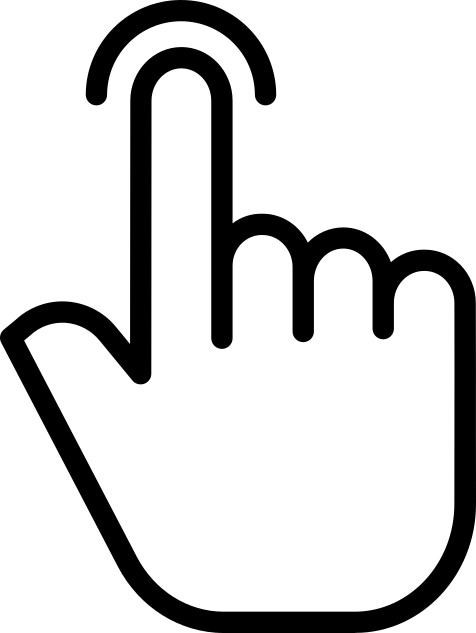
\includegraphics[width=0.03\textwidth]{static/dedo.png}} ;
         \node[factor, minimum size=1cm, xshift=3cm] (p3) {} ;
         \node[const, above=of p1, yshift=.15cm] (fp1) {$?$};
         \node[const, above=of p2, yshift=.15cm] (fp2) {$?$};
         \node[const, above=of p3, yshift=.15cm] (fp3) {$?$};
         \node[const, below=of p2, yshift=-.10cm, xshift=0.3cm] (dedo) {};
        
        } 
\end{figure}

% Parrafo

Para actualizar las creencias posiblemente nos veamos tentados a aplicar el principio de indiferencia nuevamente, asignando $0.5$ a las dos cajas que todavía ocultan información.
%
Aunque en este caso particular esa solución sea casualmente correcta para el modelo A, esa metodología conduce a errores en términos generales.
%
El principio de indiferencia sólo se aplica una única vez, al inicio.
%
Después sólo actualizaremos esa creencia en función de la nueva información que vayamos incorporando.

Para ello revisemos cuales son los caminos paralelos del modelo causal que siguen siendo compatible con el observable.
%
Para actualizar las creencias simplemente nos quedamos con la creencia previa que es compatible con el dato, $P(r_i, s_2)$.
%
\begin{table}[ht!]
\centering
$P(r=i, s=2 | \text{Modelo A})$ \hspace{2.7cm} $P(r=i, s=2 | \text{Modelo B})$ \\[0.1cm]
\begin{tabular}{|c|c|c|c||c|} \hline \setlength\tabcolsep{0.4cm}
       & \, $r_1$ \, &  \, $r_2$ \, & \, $r_3$ \, & \\ \hline 
  $s_2$ & $1/6$ & $0$ & $1/6$ & $1/3$ \\ \hline
  \end{tabular}
  \hspace{1.5cm}
  \begin{tabular}{|c|c|c|c||c|} \hline  \setlength\tabcolsep{0.4cm} 
 & \, $r_1$ \, &  \, $r_2$ \, & \, $r_3$ \, & \\ \hline 
  $s_2$ & $1/6$ & $0$ & $1/3$ & $1/2$ \\ \hline
  \end{tabular}
  \caption{La creencia conjunta y marginal que sobrevive luego de ver los datos. }
  \label{tab:creencia_compatible}
\end{table}

En la tabla~\ref{tab:creencia_compatible} nos quedamos con la creencia conjunta y marginal que sigue siendo compatible con el dato.
%
Esto es exactamente lo mismo que quedarnos con los caminos del modelo causal que son posibles dado el modelo causal y el observable.
%
En la figura~\ref{fig:caminos_compatibles} mostramos los caminos que son compatibles en negro y los incompatibles en gris.

\begin{figure}[ht!]
\centering
\begin{subfigure}[b]{0.48\textwidth}
\centering
\tikz{
\node[latent, draw=white, yshift=0.7cm] (b0) {$1$};

\node[latent,below=of b0,yshift=0.7cm, xshift=-2cm] (r1) {$r_1$};
{\color{gray}\node[latent,draw=gray,below=of b0,yshift=0.7cm] (r2) {$r_2$};}
\node[latent,below=of b0,yshift=0.7cm, xshift=2cm] (r3) {$r_3$};

\node[latent, below=of r1, draw=white, yshift=0.7cm] (br1) {$\frac{1}{3}$};
{\color{gray}\node[latent, below=of r2, draw=white, yshift=0.7cm] (br2) {$\frac{1}{3}$};}
\node[latent, below=of r3, draw=white, yshift=0.7cm] (br3) {$\frac{1}{3}$};
\node[latent,below=of br1,yshift=0.7cm, xshift=-0.5cm] (r1d2) {$s_2$};
{\color{gray}\node[latent,draw=gray,below=of br1,yshift=0.7cm, xshift=0.5cm] (r1d3) {$s_3$};}

\node[latent,below=of r1d2,yshift=0.7cm,draw=white] (br1d2) {$\frac{1}{3}\frac{1}{2}$};
{\color{gray} \node[latent,draw=gray,below=of r1d3,yshift=0.7cm, draw=white] (br1d3) {$\frac{1}{3}\frac{1}{2}$}; }
{\color{gray}\node[latent,draw=gray,below=of br2,yshift=0.7cm, xshift=-0.5cm] (r2d1) {$s_1$}; }
{\color{gray} \node[latent,draw=gray,below=of br2,yshift=0.7cm, xshift=0.5cm] (r2d3) {$s_3$}; }
{\color{gray} \node[latent,draw=gray,below=of br3,yshift=0.7cm, xshift=-0.5cm] (r3d1) {$s_1$}; }
\node[latent,below=of br3,yshift=0.7cm, xshift=0.5cm] (r3d2) {$s_2$};

{\color{gray}\node[latent,below=of r2d1,yshift=0.7cm, draw=white] (br2d1) {$\frac{1}{3}\frac{1}{2}$};}
{\color{gray}\node[latent,below=of r2d3,yshift=0.7cm,draw=white] (br2d3) {$\frac{1}{3}\frac{1}{2}$};}
{\color{gray}\node[latent,below=of r3d1,yshift=0.7cm, draw=white] (br3d1) {$\frac{1}{3}\frac{1}{2}$};}
\node[latent,below=of r3d2,yshift=0.7cm,draw=white] (br3d2) {$\frac{1}{3}\frac{1}{2}$};
\edge[-] {b0} {r1,r3};
\edge[-,draw=gray] {b0} {r2};
\edge[-] {r1} {br1};
\edge[-,draw=gray] {r2} {br2};
\edge[-] {r3} {br3};
\edge[-] {br1} {r1d2};
\edge[-,draw=gray] {br1} {r1d3};
\edge[-] {r1d2} {br1d2};
\edge[-,draw=gray] {r1d3} {br1d3};
\edge[-, draw=gray] {br2} {r2d1, r2d3};
\edge[-] {br3} {r3d2};
\edge[-, draw=gray] {br3} {r3d1};
\edge[-, draw=gray] {r2d1} {br2d1};
\edge[-, draw=gray] {r2d3} {br2d3};
\edge[-, draw=gray] {r3d1} {br3d1};
\edge[-] {r3d2} {br3d2};
}
\caption{Modelo A}
\label{fig:caminos_pre_montyhall_compatibles}
\end{subfigure}
\begin{subfigure}[b]{0.48\textwidth}
\centering
\tikz{
\node[latent, draw=white, yshift=0.7cm] (b0) {$1$};
\node[latent,below=of b0,yshift=0.7cm, xshift=-2cm] (r1) {$r_1$};
{\color{gray}\node[latent,draw=gray,below=of b0,yshift=0.7cm] (r2) {$r_2$}; }
\node[latent,below=of b0,yshift=0.7cm, xshift=2cm] (r3) {$r_3$}; 

% \node[latent, below=of r1, draw=white, yshift=0.8cm] (br1) {$\frac{1}{3}$};
% \node[latent, below=of r2, draw=white, yshift=0.8cm] (br2) {$\frac{1}{3}$};
% \node[latent, below=of r3, draw=white, yshift=0.8cm] (br3) {$\frac{1}{3}$};
% \node[latent,below=of br1,yshift=0.8cm] (c11) {$c_1$};
% \node[latent,below=of br2,yshift=0.8cm] (c12) {$c_1$};
% \node[latent,below=of br3,yshift=0.8cm] (c13) {$c_1$};

\node[latent, below=of r1, draw=white, yshift=0.7cm] (bc11) {$\frac{1}{3}$};
{\color{gray}\node[latent, below=of r2, draw=white, yshift=0.7cm] (bc12) {$\frac{1}{3}$};}
\node[latent, below=of r3, draw=white, yshift=0.7cm] (bc13) {$\frac{1}{3}$};
\node[latent,below=of bc11,yshift=0.7cm, xshift=-0.5cm] (r1d2) {$s_2$};
{\color{gray}\node[latent,draw=gray,below=of bc11,yshift=0.7cm, xshift=0.5cm] (r1d3) {$s_3$};}
{\color{gray}\node[latent, draw=gray,below=of bc12,yshift=0.7cm] (r2d3) {$s_3$};}
\node[latent,below=of bc13,yshift=0.7cm] (r3d2) {$s_2$};

\node[latent,below=of r1d2,yshift=0.7cm,draw=white] (br1d2) {$\frac{1}{3}\frac{1}{2}$};
{\color{gray}\node[latent,below=of r1d3,yshift=0.7cm, draw=white] (br1d3) {$\frac{1}{3}\frac{1}{2}$};}
{\color{gray}\node[latent,below=of r2d3,yshift=0.7cm,draw=white] (br2d3) {$\frac{1}{3}$};}
\node[latent,below=of r3d2,yshift=0.7cm,draw=white] (br3d2) {$\frac{1}{3}$};
\edge[-] {b0} {r1,r3};
\edge[-,draw=gray] {b0} {r2};
% \edge[-] {r1} {br1};
% \edge[-] {r2} {br2};
% \edge[-] {r3} {br3};
% \edge[-] {br1} {c11};
% \edge[-] {br2} {c12};
% \edge[-] {br3} {c13};
\edge[-] {r1} {bc11};
\edge[-,draw=gray] {r2} {bc12};
\edge[-] {r3} {bc13};
\edge[-] {bc11} {r1d2};
\edge[-,draw=gray] {bc11} {r1d3};
\edge[-,draw=gray] {bc12} {r2d3};
\edge[-] {bc13} {r3d2};
\edge[-] {r1d2} {br1d2};
\edge[-,draw=gray] {r1d3} {br1d3};
\edge[-,draw=gray] {r2d3} {br2d3};
\edge[-] {r3d2} {br3d2};
}
\caption{Modelo B}
\label{fig:caminos_montyhall_compatibles}
\end{subfigure}
\caption{Los caminos paralelos compatibles (negro) e incompatibles (gris) con el dato $s=2$. }
\label{fig:caminos_compatibles}
\end{figure}
% Cuando aplicamos por primera vez el principio de indiferencia en la figura \ref{fig:principio_de_indiferencia}, el espacio de hipótesis se reducía a tres opciones, una por caja.
% %
% En este caso, en el que estamos considerando una variable nueva (la señal $s$) que representa la pista, el espacio de hipótesis es otro, más grande, por lo que esta creencia a priori no nos sirve.
% %

Es decir, para actualizar nuestra creencia nos quedamos con la creencia a priori que es compatible con los datos.
%
Lo que nos permitirá cumplir el objetivo que nos habíamos propuesto, actualizar la creencia sobre el regalo luego de haber visto la pista.
%
\textbf{La creencia que sobrevive}, $P(r_i, s_2)$, es ahora nuestra nueva creencia total.
%
Para expresarla nuevamente como tal, la normalizamos para que vuelva a sumar 1.
%
\begin{equation}
P(r_i| s_2, \text{Modelo} ) = \frac{P(r_i, s_2| \text{Modelo})}{P(s_2| \text{Modelo})}
\end{equation}
%
La concusión a la que llegamos depende del modelo causal elegido.
\begin{figure}[ht!]
\centering
\begin{subfigure}[b]{0.48\textwidth}
\centering
\tikz{ %
        
         \node[factor, minimum size=1cm] (p1) {
\includegraphics[width=0.05\textwidth]{static/cerradura.png}} ;
         \node[det, minimum size=1cm, xshift=1.5cm] (p2) {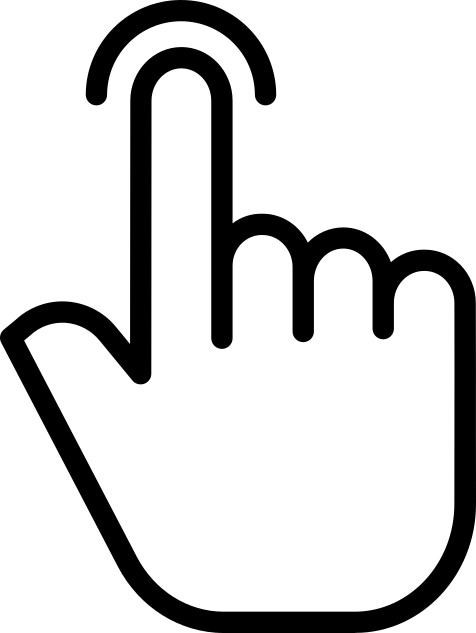
\includegraphics[width=0.06\textwidth]{static/dedo.png}} ;
         \node[factor, minimum size=1cm, xshift=3cm] (p3) {} ;

         \node[const, above=of p1, yshift=.15cm] (fp1) {$1/2$};
         \node[const, above=of p2, yshift=.15cm] (fp2) {$0$};
         \node[const, above=of p3, yshift=.15cm] (fp3) {$1/2$};
         \node[const, below=of p2, yshift=-.10cm, xshift=0.3cm] (dedo) {};
}
\caption{Modelos A}
\end{subfigure}
\begin{subfigure}[b]{0.48\textwidth}
\centering
\tikz{ %
        
         \node[factor, minimum size=1cm] (p1) {
\includegraphics[width=0.05\textwidth]{static/cerradura.png}} ;
         \node[det, minimum size=1cm, xshift=1.5cm] (p2) {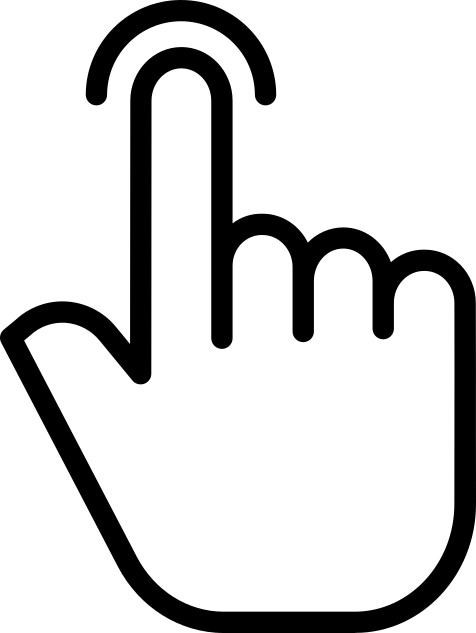
\includegraphics[width=0.06\textwidth]{static/dedo.png}} ;
         \node[factor, minimum size=1cm, xshift=3cm] (p3) {} ;
         
         \node[const, above=of p1, yshift=.15cm] (fp1) {$1/3$};
         \node[const, above=of p2, yshift=.15cm] (fp2) {$0$};
         \node[const, above=of p3, yshift=.15cm] (fp3) {$2/3$};
         \node[const, below=of p2, yshift=-.10cm, xshift=0.3cm] (dedo) {};
        }
\caption{Modelo B}
\end{subfigure}
\caption{Nueva creencia honesta dada el dato y el modelo}
\end{figure}
%  
Si bien ambas respuesta son diferentes, ambas comparten la propiedad de ser la distribución de creencias que maximiza la incertidumbre dada la evidencia formal (modelo causal) y empírica (datos), lo que hace que sean proposiciones sobre las que podemos acordar tanto intercultural como intersubjetivamente.


\section{Las reglas de la probabilidad}\label{sec:reglas_de_la_probabilidad}

La teoría de la probabilidad es actualmente el enfoque utilizado para representar incertidumbre asociada al conocimiento empírico.
%
La teoría de la probabilidad tiene puede resumirse en dos reglas, conocidas como la regla de la suma y la regla del producto.
%
La regla de la suma proviene del principio de integridad y establece que cualquier creencia marginal puede ser obtenida integrando la creencia conjunta.
%
\begin{equation}
P(r_i) = \sum_j P(r_i, s_j)
\end{equation}
%
La segunda regla proviene del principio de coherencia y, expresada como producto, establece que cualquier distribución conjunta puede ser expresada como el producto de distribuciones condicionales uni-dimensionles.
%
\begin{equation}
P(s_j)P(r_i|s_j) = P(r_i, s_j)
\end{equation}

% Parrafo

Las reglas de la probabilidad han sido derivadas formalmente a partir de una gran cantidad de sistemas axiomáticos conceptualmente distintos e independientes entre si, lo cual es uno de los puntos fuertes a su favor~\cite{halpern2017}.
%
El sistema axiomático de Cox~\cite{cox} las deriva a partir de principios más generales aun de los propuestos en la sección anterior.
%
El sistema axiomático de Ramsey~\cite{ramsey} las deriva haciendo una analogía con los pagos que aceptaríamos en una apuesta, de forma similar a lo que veremos en la siguiente sección. 
%
El sistema axiomático de Kolmogorv~\cite{kolmogorov} tiene una motivación filosófica menos explícita, pero su simplicidad matemática hace que sea el sistema axiomático de referencia.
%
En el sistema de Kolmogorov la regla de la suma forma parte de los axiomas y la regla del producto de una definición complementaria.
%
\begin{quotation}
Sea $E$ un conjunto de elementos $e_1, e_2, \dots$, y $F$ conjunto de subconjuntos de $E$.
%
\begin{enumerate}\itemsep-0.05cm
\item $F$ está cerrada bajo complementos, uniones e intersecciones contables.
\item $F$ contiene al conjunto $E$
\item Todo conjunto $S \in F$ se le asigna una número real no negativo, $P(S)$.
\item $P(E) = 1$
\item Si $S_1, S_2, \dots$ son conjuntos mutuamente excluyente, luego
\begin{equation}
P(S_1 \cup S_2 \cup \dots ) = \sum P(S_i)
\end{equation}
\end{enumerate}
\end{quotation}
%
La regla de la suma se deriva inmediatamente del axioma 5 dado que siempre podemos expresar cualquier conjunto como $A = A \cap (B \cup \neg B)$.
%
La probabilidad condicional (o regla del producto) se incluye en el sistema como una definición que cumple con los axiomas de la probabilidad. 

% %Ciertamentese ha dedicado mucho más esfuerzo a justificar la teoría de la probabilidad que cualquier otro enfoque para representar la incertidumbre y el tiempo dirá si se pueden se pueden desarrollar otros enfoques superadores.
% Pero quizás más importante es que su aplicación estricta (lo que llamamos inferencia Bayesiana) garantiza los acuerdos intersubjetivos a través de la maximización de la incertidumbre (entropía) dada la información empírica y formal (datos y modelos causales)~\cite{Jaynes2003}.
% %

% Parrafo

Así expresada, la teoría de la probabilidad está basada en sólo dos de los cuatro principios vistos anteriormente, y carace de criterio para definir distribuciones de creencias iniciales (inferencia Bayesiana) y para expresar relaciones causales (inferencia causal).

\subsection{Teorema de Bayes}

El teorema de Bayes no es más que un corolario de las reglas de las probabilidad, que surge de aplicar dos veces la regla del producto.
%
Usando las variables vistas en la sección anterior, el teorema de Bayes puede expresarse como,
\begin{equation}
\begin{split}
P(r_i|s_2) = \frac{P(r_i, s_2)}{P(s_2)} = \frac{P(s_2|r_i)P(r_i)}{P(s_2)} 
\end{split}
\end{equation}
%
Es una práctica muy común no expresar explícitamente que esas probabilidades en realidad dependen de un cierto modelo causal, por lo que lo correcto sería incluirlo en el condicional.
%
Notar además que escribimos a $r$ con un subíndice $i$ y a $s$ con un subíndice $2$.
%
Con esto queremos connotar la idea de que $r_i$ es una variable libre, que queremos evaluar para los diferentes valores (la hipótesis), y $s_2$ es un valor constante (el dato observado).
%
En línea con esta interpretación, volvemos a expresar el teorema de Bayes de la siguiente manera.
% %
% \begin{equation*}
% \underbrace{P(\text{Hip\'otesis }|\text{ Datos})}_{\text{\scriptsize Posteriori}} = \frac{\overbrace{P(\text{Datos }|\text{ Hip\'otesis})}^{\text{\scriptsize Verosimilitud}} \overbrace{P(\text{Hip\'otesis})}^{\text{\scriptsize Priori}} }{\underbrace{P(\text{Datos})}_{\text{\scriptsize Evidencia}}}
% \end{equation*}
%
\begin{equation*}
\underbrace{P(\text{Hip\'otesis }|\text{ Datos, Modelo})}_{\text{\scriptsize Posterior}} = \frac{\overbrace{P(\text{Datos }|\text{ Hip\'otesis, Modelo})}^{\text{\scriptsize Verosimilitud}} \overbrace{P(\text{Hip\'otesis }|\text{ Modelo})}^{\text{\scriptsize Prior}} }{\underbrace{P(\text{Datos }|\text{ Modelo})}_{\text{\scriptsize Evidencia}}}
\end{equation*}
%
Los diferentes factores del teorema de Bayes han recibido nombres a lo largo de la historia, que revisemos a continuación.

\subsubsection*{Prior}

El \emph{prior} es la distribución de creencia inicial de las hipótesis dado el modelo causal antes de ver los datos.
%
En la sección \emph{\nameref{sec:principio_indiferencia}} hemos visto un criterio intercultural que nos permite alcanzar un primer acuerdo intersubjetivo en contextos de incertidumbre.
%
El enfoque ``frecuentista'' de la teoría de la probabilidad que rechaza todo criterio para definir distribuciones de creencias iniciales se ve impedido de utilizar el teorema de Bayes.
%
Como consecuencia, en vez de ofrecer distribuciones de probabilidad sobre todo el espacio de hipótesis, seleccionan una única hipótesis (estimación puntual) en base a funciones de costo ad-hoc, siendo las más común la maximización de la verosimilitud.

\subsubsection*{Verosimilitud}

La \emph{verosimilitud} es la predicción del dato observado cuando suponemos que la hipótesis que estamos evaluando es cierta.
%
Veamos cuál es la verosimilitud, $P(s2|r_i, \text{Modelo B})$, la probabilidad de que la pista haya señalado la caja $2$ en el modelo de Monty Hall para las diferentes posibles posiciones del regalo $r_i$.
%
\begin{figure}[ht!]
\begin{subfigure}[b]{0.7\textwidth}
\centering
\tikz{
\phantom{\node[latent, draw=white, yshift=0.8cm] (b0) {$1$};}
\node[latent,below=of b0,yshift=0.8cm, xshift=-2.5cm] (r1) {$r_1$};
\node[latent,below=of b0,yshift=0.8cm] (r2) {$r_2$};
\node[latent,below=of b0,yshift=0.8cm, xshift=1.8cm] (r3) {$r_3$};

\node[latent, below=of r1, draw=white, yshift=0.8cm] (br1) {$1$};
\node[latent, below=of r2, draw=white, yshift=0.8cm] (br2) {$1$};
\node[latent, below=of r3, draw=white, yshift=0.8cm] (br3) {$1$};

\node[latent,below=of br1,yshift=0.8cm, xshift=-0.7cm] (r1d2) {$s_2$};
\node[latent,below=of br1,yshift=0.8cm, xshift=0.7cm] (r1d3) {$s_3$};
\node[latent,below=of br2,yshift=0.8cm] (r2d3) {$s_3$};
\node[latent,below=of br3,yshift=0.8cm] (r3d2) {$s_2$};

\node[latent,below=of r1d2,yshift=0.8cm,draw=white] (br1d2) {$\frac{1}{2}$};
\node[latent,below=of r1d3,yshift=0.8cm, draw=white] (br1d3) {$\frac{1}{2}$};
\node[latent,below=of r2d3,yshift=0.8cm,draw=white] (br2d3) {$1$};
\node[latent,below=of r3d2,yshift=0.8cm,draw=white] (br3d2) {$1$};
\phantom{\edge[-] {b0} {r1,r2,r3};}
\edge[-] {r1} {br1};
\edge[-] {r2} {br2};
\edge[-] {r3} {br3};
\edge[-] {br1} {r1d2,r1d3};
\edge[-] {br2} {r2d3};
\edge[-] {br3} {r3d2};
\edge[-] {r1d2} {br1d2};
\edge[-] {r1d3} {br1d3};
\edge[-] {r2d3} {br2d3};
\edge[-] {r3d2} {br3d2};
}
\caption{Modelos causales B cuando conocemos la posición del regalo.}
\end{subfigure}
\begin{subfigure}[b]{0.29\textwidth}
\centering
 $P(s_2|r_i,\text{Modelo B})$   
 
 \begin{tabular}{c|c|c|c} \setlength\tabcolsep{0.4cm} 
          & \, $r_1$ \, &  \, $r_2$ \, & \, $r_3$ \, \\ \hline 
   $s_2$ & $1/2$ & $0$ & $1$  \\ \hline
\end{tabular}
\vspace{1cm}
\caption{Verosimilitud}
\end{subfigure}   
\caption{Predicción del dato observado dado que el modelo causal B y la hipótesis son ciertas. }
\end{figure}

%

Cuando el regalo está en la misma posición que la caja elegida $r=c=1$, el modelo causal permite que la pista señale cualquiera de la otras dos cajas, por lo que la creencia a priori de que la caja señalada sea la $s=2$ es $1/2$.
%
Cuando el regalo está en una caja distinta a la elegida $r\neq c$, el modelo causal limita la pista a una única caja.
%
Si el regalo está en la caja $r=2$, la creencia a priori de que la caja señalada sea la $s=2$ es $0$.
%
Y si el regalo está en la caja $r=3$, la creencia a priori de que la caja señalada sea la $s=2$ es $1$.

\subsubsection*{Posterior}

En la sección \emph{\nameref{sec:principio_choerencia}} vimos que la nueva creencia no es más que la creencia previa que sigue siendo compatible con el dato.
%
El teorema de Bayes nos permite ahora reconocer que la sorpresa que produce el dato observado es lo que actúa como filtro de las creencias previas.
%
Debido a que el denominador del teorema de Bayes es constante, la distribución de creencias a posteriori es proporcional al producto entre el prior y la verosimilitud.
%
\begin{table}[ht!]
\centering

$P(r_i|s_2, \text{M}_B) \propto P(r_i| \text{M}_B) P(s_2|r_i, \text{M}_B) $ \\[0.2cm]

\begin{tabular}{l|c|c|c} \setlength\tabcolsep{0.4cm} 
          & \, $r_1$ \, &  \, $r_2$ \, & \, $r_3$ \, \\ \hline 
   $P(s_2|r_i,\text{M}_B)$ & $1/2$ & $0$ & $1$  \\ \hline
   $P(r_i,\text{M}_B)$ & $1/3$ & $1/3$ & $1/3$  \\ \hline
   $P(r_i|s_2,\text{M}_B) \propto$ & $1/6$ & $0$ & $1/3$\\ \hline
\end{tabular}
\end{table}

% Parrafo

Como las verosimilitudes son predicciones, sus valores van entre $0$ y $1$.
%
Si la hipótesis $r=2$ fuera cierta, la sorpresa producida cuando observamos que la pista señala la caja $s=2$ sería total.
%
En ese caso, como la predicción del dato observado es $0$, nada del la creencia priori sobre $r=2$ pasa a la creencia a posteriori.
%
So la hipótesis $r=3$ fuera cierta, la sorpresa producida cuando observamos que la pista señala la caja $s=2$ es nula.
%
En ese caso, como la predicción del dato observado es $1$, toda la creencia priori sobre $r=2$ pasa a la creencia a posteriori.

% Parrafo

En inferencia Bayesiana entonces, la verosimilitud funciona como el filtro de las creencias previas. 

\subsubsection*{Evidencia}

De forma similar a la verosimilitud, la evidencia es una predicción a priori del dato observado, pere que está hecha con la contribución de todas las hipótesis.
%
Por la reglas de la probabilidad, el denominador del teorema de Bayes puede expresarse como una suma sobre todos los posibles valores del numerador, uno por cada hipótesis.
%
Esto hace que la evidencia sea constante para las diferentes hipótesis, por lo que puede ser ignorado cuando se comparan hipótesis alternativas.
%
Sin embargo, la evidencia va a ser distinta para los diferentes modelos.
%
En el modelo B la predicción a priori de que la caja señalada sea $s=2$, integrando todas las hipótesis, es $1/2$. 
%
\begin{equation}
P(s_2|M_B) = \sum_i P(s_2|r_i, M_B) P(r_i, M_B) = \frac{1}{2} \frac{1}{3} + 0 \frac{1}{3} + \frac{1}{1} \frac{1}{3} = 1/2 
\end{equation}
%
Mientras que en el modelo A la predicción a priori de que la caja señalada sea $s=2$, integrando todas las hipótesis, es $1/3$. 
%
\begin{equation}
P(s_2|M_A) = \sum_i P(s_2,r_i| M_A) = 1/3 
\end{equation}
%
Lo que ya había sido calculado previamente en las marginales de la tabla \ref{tab:creencia_marginal}.

% Parrafo

La evidencia será de interés cuando queramos evaluar modelos causales alternativos.
%
En la sección \ref{sec:modelos_alternativos} mostramos en un ejemplo cómo deben evaluarse modelos causales alternativos aplicando estrictamente las reglas de la probabilidad.


\subsection{Notas sobre las interpretaciones de la probabilidad}
% 
% \subsection{La escuela naturalista (frecuentista)}
% 
% \subsection{La escuela epistémica (Bayesiana)}

Incluso las ciencias matemáticas, en contacto con problemas empíricos, produjo diversas escuelas de pensamiento a pesar de estar regidas supuestamente bajo las mismas reglas teóricas.
%
La justificación axiomática de la teoría de la probabilidad no ha sido suficiente para unificar su interpretación.
%
El debate filosófico de fondo respecto de las interpretaciones de la probabilidad tiene que ver con la solución que las dos principales escuelas le dieron al problema de la contradicción: la epistémica (bayesiana) y la ontológica (frecuentista).

% Parrafo

En el siglo 18 el concepto de probabilidad comenzó a usarse en Europa para expresar creencias contradictorias en contextos de incertidumbre.
%
Laplace, quién tenía la convicción de que el mundo era determinista, no podía más que utilizar la probabilidad para expresar grados de creencia a hipótesis mutuamente contradictorias.
%
En un mundo determinista no es posible que A y no A puedan ocurrir dadas exactamente las mismas condiciones iniciales del mundo.
%
Bajo este marco, la contradicción de creer simultanemente en A y no A es sólo una expresión de nuestra incertidumbre.
%
Más allá de la creencia particular de Laplace, la solución epistémica de la contradicción nada dice de la naturaleza (u ontología) del mundo.

% Parrafo

La solución epistémica, que proponía creer simultaneamente en hipótesis mutuamente contradictorias, fue el motivo por el cual la corriente bayesiana de la teoría de la probabilidad fue tan combatida a finales del siglo 19 y durante casi todo el siglo 20.
%
A diferencia de las tradiciones filosóficas de origen oriental y americano, que ya admitían algún tipo de contradicción en su sistema de creencias, la tradición filosófica Europea la rechazaba por completo.

% Parrafo

La escuela frecuentista, tal como se enseña en la materia probabilidad y estadísitica de la facultad de ciencias exactas y naturales, define a la probabilidad como el número al que tiende una frecuencia obtenida luego de realizar varios ``experimentos independientes'' bajo ``las mismas condiciones''.
%
Según esta corriente la probabilidad de eventos deterministas, por ejemplo de que exista un planeta no detectado en el sistema solar, es 0 o 1 aunque no conozcamos su valor.
%
Sólo los objetos no deterministas, que llaman ``variables aleatorias'', tienen valores intermedios que representan la frecuencia en la que los diferentes estado del universo se producen a partir de exactamente las mismas condiciones inciales.
%
De esta forma, la contradicción se propone como una propiedad externa al sistema lógico, propia de la naturaleza del mundo.
%
La escuela frecuentista, para evitar la contradicción en sus sistema lógico, se ve obligada a afirmar la naturaleza aleatoria del mundo, lo que representa una la solución ontólógica de la contracción.

\section{La función de costo epistémica universal}

Lo que veremos en esta sección es que la natrualeza multiplicativa de los procesos de selección evolutiva y probabilistica tiene una serie de propiedades que garantizan la adquisición de conocimiento empírico.

% Parrafo

La interpretación ontológica de la teoría de la probabilidad, al rechazar la contradicción epistémica, se ve impedida de definir probabilidades iniciales no justificadas observacionalmente (prior), y por lo tanto de utilizar el teorema de Bayes.
%
Como consecuencia, en vez de ofrecer distribuciones de probabilidad sobre todo el espacio de hipótesis, el enfoque frecuentista suele seleccionar una única hipótesis (estimación puntual) en base a funciones de costo ad-hoc.
%
La función de costo más utilizada por la corriente frecuentista es la maximización de la verosimilitud.
%
Este enfoque a mostrado tener una serie de problemas siendo el más conocido el problema del sobreajuste (o overfitting).
%
Para corregir este problema se han desarrollado otras funciones de costo ad-hoc que incluyen la penalización por complejidad del modelo, y la separación de los datos con objetivos de ``entrenamiento'' y ``validación''.
%
A pesar de que estas metodologías permiten desarrollar redes neuronales modernas, ellas sufren en general de problemas de calibración. 

% Parrafo

John Larry Kelly (Jr) comienza en su artículo ``A New Interpretation of Information Rate'' para los laboratorios Bell (1956) diciendo, 
%
\begin{quotation}
The author believes that [the cost function approach] it is too general to shed any light on the specific problems of communication theory. (...). The point here is that an arbitrary combination of a statistical transducer (i.e., a channel) and a cost function does not necessarily constitute a communication system. (...). The situation which will be chosen here is one in which a gambler uses knowledge of the received symbols of a communication channel in order to make profitable bets on the transmitted symbols.
\end{quotation}
%
En otras palabras, no toda función de costo garantiza la adquisición de conocimiento empírico.

% Parrafo

Kelly considera un escenario en el que una casa de apuestas ofrece pagos $Q_c$ y $Q_s$ por Cara y Seca: por cada unidad apostada la casa devuelve $Q$ si ocurre el evento apostado y $0$ en caso contrario.
%
La pregunta que él se hace es: ¿Cuál es la mejor forma de apostar?

% Parrafo

Supongamos que se conoce la frecuencia típica $p$ de Cara, y $1-p$ de Seca de una moneda.
%
El juego propuesto por Kelly entre la casa de apuestas y les apostadores sigue las reglas típicas de la vida real.
%
Toda persona comienza con una riqueza $\omega_0$.
% %
En cada ronda, la persona apuesta una proporción $b_c$ a Cara y $b_s$ a Seca.
% 
% % Parrafo
% 
% Hay dos formas de apostar.
% %
% La primera es apostar a una única de las dos opciones, por ejemplo a Caras.
% %
% En este escenario, la persona asigna un valor $ 1 \geq b_c = l > 0 $ a Caras y $b_s = 0$ a secas.
% %
% Supongamos que en la primera sale Cara y en la segunda Seca.
% %
% La riqueza en la primera es el ahorro $1-l$ más el pago que obtiene por lo apostado en Cara $l \, Q_c$.
% %
% Y en la segunda vuelta, cuando sale Seca, la riqueza es solo el ahorro, lo no apostado a Cara $1-l$.
% %
% \begin{equation}
% \omega_T = \underbrace{\overbrace{(\omega_0 \, (1-l) + \omega_0 \, l \, Q_c )}^{\omega_1} \, (1-l)}_{\omega_2} \,\dots
% \end{equation}
% %
% Lo que podemos reescribir como,
% %
% \begin{equation}
% \begin{split}
% \omega_T &= \omega_0 \, ((1-l) + \, l \, Q_c ) \, (1-l) \, \dots \\
%  &= \omega_0 \, ( (1-l) + \, l \, Q_c )^{n_c} \, (1-l)^{n_s} 
% \end{split}
% \end{equation}
% %
% donde $n_c + n_s = T$ son la cantidad de veces que salió Cara y Seca en los $T$ pasos.
% %
% Es decir, la riqueza se actualiza siguiendo un proceso multiplicativo.
% 
% % Parrafo
% 
% La otra forma de apostar consiste en utilizar todos los recursos en cada vuelta, poniendo $b_c = b$ en Cara y el resto en Seca $b_s = (1-b)$.
% %
% En este caso la riqueza se actualiza como,
% %
% \begin{equation} \label{eq:kelly_paraconsistente}
% \omega_T = \underbrace{\overbrace{(\omega_0 \, b \, Q_c)}^{\omega_1} \,  (1-b) \, Q_s}_{\omega_2} \dots = \omega_0 (b \, Q_c)^{n_c} ((1-b) \, Q_s )^{n_s}
% \end{equation}
% %
% No sólo las dos formas de apostar actualizan los recursos a través de un proceso multiplicativo. 
% %
% No es difícil demostrar que siempre existe una equivalencia.
% %
% Por ello, de aquí en adelante analizaremos únicamente esta última forma de apuestar, la que utiliza todos los recursos en cada vuelta.
% 
% % Parrafo
% 
% ¿Cuáles son los pagos que puede ofrecer una casa de apuestas?
% %
% Supongamos que la casa de apuestas ofrece pagos basados en el principio de reciprocidad analizados por Pascal y Fermat (figura \ref{fig:pascal-fermat}).
% %
% Según este principio, la pago justa debe ser inversamente proporcional a la probabilidad.
% %
% Por ejemplo, si la probabilidad de Seca es $(1-p) = 1/4$, y apostamos una unidad a Seca en cada vuelta, $3$ de cada $4$ veces vamos a perder y solo una vamos a ganar.
% %
% Luego, para que el intercambio sea ``justo'' (nadie gane), la casa de apuestas tiene que multiplicar por $Q_s = 4$ el valor apostado a Secas.
% %
% Lo mismo ocurre en Caras, $Q_c = 1/p$.
% 
% % Parrafo
% 
% En general, la casa de apuesta puede ofrecer cualquier tipo de pago.
% %
% Por ejemplo, pagos justos pero sesgados, basados en una probabilidad $q$ distinta de $p$, $Q_c = 1/q$ y $Q_s = 1/(1-q)$.
% %
% O incluso ofrecer pagos sesgados, basados en $q$, y no recíprocos que incluyen una comisión $c$, $Q_c = (1/q)\,(q\,c)$, $Q_c = (1/(1-q))\,((1-q)\,c)$.
% %
% Cuando $c = 1$, la comisión es total y tanto en Cara como en Seca la casa de apuestas simplemente devuelve los recursos apostados en la opción ganadora, $Q_c = Q_s = 1$.
% %
% Si bien en este caso no habría ningún incentivo para apostar, es interesante en tanto será (a partir del principio de coherencia que veremos en la siguiente sección) la forma natural de evaluar las hipótesis. 
% 
% % Parrafo
% 
% La tasa de crecimiento individal para cualquier tipo de pago tal que $Q_c > 0$ y $Q_s > 0$ es
% %
% \begin{equation}
% \begin{split}
% \lim_{T \rightarrow \infty } (\omega_0 \, r)^T &= \omega_0 (b \, Q_c)^{n_c} ((1-b) \, Q_s )^{n_s} \\
% r &= \lim_{T \rightarrow \infty } (b \, Q_c)^{\frac{n_c}{T}} ((1-b) \, Q_s )^{\frac{n_s}{T}} = (b \, Q_c)^{p} ((1-b) \, Q_s )^{1-p}
% \end{split}
% \end{equation}
% %
% Para maximizar $r$ tomamos el logaritmo de ambos lados, y buscamos el punto crítico de esta función cóncava,
% %
% \begin{equation}
% \begin{split}
% 0 &= \frac{d}{db} p \log (b \, Q_c) + (1-p) \log ((1-b) \, Q_s) \\
% 0 &= \frac{p}{b} + \frac{1-p}{1-b} \\
% p &= b 
% \end{split}
% \end{equation}
% %
% Sin importar el pago que elija la casa de apuestas, individualmente la tasa de crecimiento siempre se maximiza dividiendo los recursos en la misma proproción que la frecuencia típica $p$.
% %
% Pero no sólo pasa esto con el máximo, la derivada de la función tampoco depende de los pagos que ofrezca la casa de apuestas.
% %
% Este resultado Kelly lo escribe con un signo de admiración.
% %
% \begin{quotation}
% That is, \emph{the gambler ignores the posted odds} in placing his bets!
% \end{quotation}
% 
% % Parrafo
% 
% En este proceso antagónico ambos agentes pueden descubrir la verdadera probabilidad a partir de la ignoracia mutua, sin necesidad de que nadie conozca la probabilidad real.
% %
% A través de los resultados obtenidos en un juegos de apuestas podemos realizar ``inferencia''.
% % 
% El uso de las funciones de costo definidas de forma para resolver problemas de aprendizaje estadísitico es una práctica común.
% %
% El problema general del enfoque basado en funciones de costo ad-hoc tiene que ver con la influencia no deseada que decisiones arbitrarias tienen sobre las distribución de los recursos entre las hipótesis y por lo tanto sobre el resultado final de la inferencia.
% 
% % Parrafo
% 
% En este sentido, los procesos multiplicativos pueden ser vistos como la función de costo universal.
% %
% A diferencia del resto de las funciones de costo, los procesos multiplicativos tienen la propiedad especial de producir, no solo una distribución de recursos independiente de los pagos arbitrarios elegidos por la casa de apuestas (o les investigadores), sino que garantiza que en tiempo infinito la hipótesis que dividió los recursos en la misma proporción que la frecuencia típica se habrá quedado con todos los recursos que tenían las otras hipótesis.
% %
% Esto es interesante en tanto será todas las axiomatizaciones alternativas de la teoría de la probabilidad llegan a la conclusión de que la forma natural de evaluar las hipótesis es a través de un proceso multiplicativo, la ``regla del producto''.
% 
% % Parrafo
% 
% En la sección anterior analizamos las consecuencias de algunos sistemas multiplicativos.
% %
% Individualmente encontramos una ventaja a favor de lo que llamamos estrategias ``equilibradas'', que dividen los recursos en la misma proporción que la frecuencia $p$ (verificado nuevamente en esta sección).
% %
% Pero además observamos una ventaja a favor de los comportamientos cooperativos: una grupo de agentes, reduciendo las fluctuaciones individuales a través de un fondo común, logran aumentar la tasas de crecimiento hasta alcanzar, en grupos grandes, tasas equivalente al promedio aritmético de los pagos que siempre es mayor que el óptimo individual.
% %
% Pero además, una vez que surge la cooperación, el grupo de agentes puede obtener una tasa de crecimiento aún mayor a través de la especialización, asignando más recursos que al estado más frecuente de lo que conviene según la frecuencia típica $p$. 
% 
% % Parrafo
% 
% La capacidad de aumentar la tasa de crecimiento a través de la cooperación y la especialización no fue analizada por Kelly, lo que abre las siguientes preguntas.
% %
% ¿Existe un conjunto de pagos $Q_c$ y $Q_s$ que garantice la coexistencia en el tiempo entre la casa de apuestas y una población de apostadoras, o siempre se puede hacer quebrar a la casa de apuestas a través de la cooperación y la especialización?
% 
% % Parrafo
% 
% Para analizar las apuestas óptimas en grupos coopertaivos debemos analizar el comportamiento del fondo común del cual dependen sus miembros.
% %
% En cada ronda, una cantidad $n_c$ de miembros van a recibir Caras y una cantidad $n_s$ va a recibir Secas.
% %
% El fondo común en un tiempo $t+1$ es la suma de todos los recursos individuales en el tiempo $t$.
% %
% Cuando el tamaño del grupo tiende a infinito, la cuota que se recibe del fondo común $\omega_{t+1}$ es equivalente al promedio de los estados.
% %
% \begin{equation}
% \begin{split}
% \lim_{N \rightarrow \infty} N \omega_{t+1} &= (\omega_t \, b \, Q_c ) \, n_c + (\omega_t \, (1-b) \, Q_s ) \, n_s \\
%  \omega_{t+1} &=  \omega_t \, \underbrace{\left(  b \, Q_c \, p +  (1-b) \, Q_s \, (1-p) \right)}_{\text{Tasa de crecimiento } r} 
% \end{split}
% \end{equation}
% %
% Si el pago es recíproco, $Q_c = 1/p$ y $Q_s = 1/(1-p)$, la tasa de crecimiento de la cuota del fondo común siempre vale $1$, más allá de la apuesta $b$ que elija el grupo coopertaivo!
% \begin{equation}
% \begin{split}
% r &=  b \, \frac{1}{p} \, p +  (1-b) \, \frac{1}{1-p} \, (1-p) = b + (1 - b) = 1
% \end{split}
% \end{equation}
% %
% Cooperar tiene una ventaja respecto de jugar individualmente, no importa si la apuesta es incorrecta, los individuos del grupo cooperativo nunca pierden.
% 
% % Parrafo
% 
% Los pago recíprocos garantizan entonces la coexistencia de una casa de apuestas con un grupo cooperativo.
% %
% Todo otro pago que ofrezca la casa de apuestas puede ser aprovechado por el grupo cooperativo.
% %
% Y a través de la especialización podrán obtener una tasa de crecimiento mayor que los agentes individuales, como vimos en la sección anterior.
% %
% Si bien la cooperación es útil para reducir fluctuaciones y aumentar la tasa de crecimiento en un juego de apuestas, jugar de forma cooperativa elimina la propiedad fundamental que hace de los procesos multiplicativos un función de costo útil como mecanismo de inferencia: la apuesta óptima ya no será aquella que divide los recursos en la misma proporción que la frecuencia típica.




\section{Selección intersubjetiva de modelos causales}\label{sec:modelos_alternativos}

\en{To evaluate the models we must calculate their probability given the data, }%
\es{Para evaluar los modelos debemos calcular su probabilidad dados los datos, }%
%
\begin{equation}
 P(\text{Model\es{o}}|\text{Dat\en{a}\es{os}}) = \frac{P(\text{Dat\en{a}\es{os}}|\text{Model\es{o}})P(\text{Model\es{o}})}{P(\text{Dat\en{a}\es{os}})}
\end{equation}

En la siguiente figura hacemos selección de los modelo causales alternativos discutidos en este capítulo (Figura~\ref{fig:modelos_alternativos}).

\begin{figure}[H]
    \centering
    \begin{subfigure}[b]{0.5\textwidth}
    \includegraphics[width=\linewidth]{figures/monty_hall_selection.pdf}
    \end{subfigure}
    \caption{
    Selección de modelos alternativos
    }
    \label{fig:estrategias_individuales}
\end{figure}

Con 32 observaciones es casi seguro que el modelo causal B es el que representa el modelo verdadero del programa Monty Hall.

(Sin terminar)

\section{Construcción de datos de base empírica metodológica} \label{sec:base_empirica_metodo}


\subsection{Los datos como funciones empíricas}

Los datos pueden ser vistos como funciones empíricas, $f(x)=y$, a través de las cuales podemos afirmar, por ejemplo, que la habilidad de Maradona fue superior a la de Messi.
\begin{equation}\label{eq:opiniones}
 \emph{Habilidad}(\text{Maradona}) > \emph{Habilidad}(\text{Messi})
\end{equation}
En este caso, la función \emph{Habilidad} representa una cierta variable (V) o característica, que aplicada sobre una unidad de análisis (UA) particular devuelve siempre un mismo resultado (R) .

% Parrafo 

Si bien las proposiciones de la ecuación \ref{eq:opiniones} tienen una estructura funcional, al conversar informalmente no hacemos explícita la definición precisa de la función.
Ahí radica el origen de muchos de los desacuerdos que tenemos cuando conversamos informalmente, porque usamos las mismas palabras para comunicar conceptos que en el fondo son distintos.
El significado preciso del dato depende entonces de la operacionalización de la función.
Por este motivo Juan Samaja propone que la estructura de todo dato científico contiene un cuarto elemento: el esquema indicidor.
Esta es la estructura invariante de todo dato (Hipótesis de Samaja).

\begin{table}[ht!]
\centering
\begin{tabular}{clcccc}
Resultado (R) & \multicolumn{1}{r|}{} &  & Variable (V) &  &  \multicolumn{1}{|c}{Unidad de Análisis (UA)} \\ \hline
   &  \multicolumn{1}{r|}{}    &  & Dimensiones (D) &  & \multicolumn{1}{|r}{} \\
                 Indicador (I)  &   & =  &  &  &  Fuente de datos (F) \\
 & \multicolumn{1}{r|}{} &  & Procedimientos (P) &        &    \multicolumn{1}{|r}{}  
\end{tabular}
\caption{Estructura invariante del todo dato empírico propuesta por Juan Samaja.}
\label{tab:matriz_datos}
\end{table}

Todo esquema indicador se compone de dimensiones (D), que son especificaciones de la variable, y de procedimientos (P) protocolos, acciones a efectuar sobre cierta fuente de datos (F).
Las reacciones del mundo natural son los indicadores (I), objetos perceptibles desde el sentido común, que interpretados con alguna hipótesis se tranforman en los resultados (R) de la variable (V).

% Parrafo

El contenido de cada uno de sus elementos depende de una serie de supuestos.
La validez interna de un dato depende en gran medida de las dimensiones (D) elegidas, de que estas expresen fielmente el concepto de la variable, que expresen lo relevante de ella y sólo de ella, discriminado factores ajenos que puedan intervenir de manera no advertida.
El proceso de selección de las dimensiones de la variable, y el conjunto de hipótesis asociaciadas, se llama examen de \emph{representatividad}.
La etapa de identificación de la fuente de datos (F), que está basa en hipótesis acerca de la autenticidad y accesibilidad de la información, se conoce como examen de \emph{viabilidad}.
La confiabilidad del dato, por su parte, depende de que los procedimientos detecten sólo esa dimensión de la fuente y no otros estímulos asociados, y de discriminar mínimas cantidades.
La definición de los protocolos (P), y sus hipótesis, se denomina examen de \emph{confiabilidad}.
Finalmente, para pasar del indicador al resultado necesitamos una última hipótesis: la hipótesis indiciadora.
En la sección \nameref{sec:principio_evidencia} veremos que existe una hipótesis indicadora general que nos permite incorporar información de los observables en nuestras distribuciones de creencia garantizando los acuerdos intersubjetivos.

Es cualquier caso, todos los datos están cargados de hipótesis.
Para que ellos puedan actuar como base empírica sobre la que se evalúan las teorías científicas es necesario que sus supuestos queden, al menos por un cierto momento, fuera de toda duda.
En este sentido, la base empírica puede ampliarse o reducirse según el conjunto de supuestos que una comunidad esté dispuesta a admitir sin poner en duda.
Para aceptar la entidad de nuestros objetos más cotidianos, como por ejemplo el precio al que ayer nos vendieron los tomates en la verdulería, o el resultado de la final de los últimos mundiales de fútbol, son suficientes los supuestos del sentido común.
No hay mayor controversia al respecto.
Este nivel de acuerdo se lo conoce como \emph{base empírica epistemológica}~\cite{klimovsky1994-desventuras}.% al cual pertenecen los observables de la sección \nameref{sec:principios_interculturales}.

Sin embargo, la ciencia construye ``datos'' que requieren suponer verdaderas ciertas teorías o técnicas especiales, como por ejemplo la inflación general del último mes en Argentina, o la habilidad que Maradona y Messi tenían cuando jugaron la final del mundial.
Un dato es depende de una teoría T si no se puede determinar sin presuponer la aplicabilidad de T, si todo procedimiento para su determinación la presupone; y puede obtenerse sin presuponer tal teoría, si tiene algún procedimiento de determinación T-independiente, por más que también tenga otros procedimientos T-dependientes~\cite{lorenzano2002-concepcionEstructuralista}.

Los acuerdos que se alcanzan en este nivel se conocen como \emph{base empírica metodológica}.
Para ello se requiere una evaluación que garantice los acuerdos intersubjetivos en la selección de los modelos causales alternativos.
En la sección ``\nameref{sec:modelos_alternativos}'' mostramos cómo evaluar modelos garatizando los acuerdos intersubjetivos.
En el capítulo \ref{ch:ttt} seleccionamos el modelo de estimación de habilidad estado-del-arte en la industria del video juego, conocido como TrueSkill Through Time (TTT).

\begin{figure}[H]
    \centering
    \begin{subfigure}[b]{0.48\textwidth}
    \includegraphics[page=3,width=\linewidth]{figures/baseEmpirica.pdf}
    \end{subfigure}
    \caption{Niveles de base empírica. En negro la base empírica epistemológica, en gris la base empírica metodológica, y en blanco los datos que todavía no han alcanzado un acuerdo intersubjetivo amplio. }
\end{figure}

En el modelo causal TTT los resultados de las partidas son la base empírica epistemológica a partir de la cual se infieren las distribuciones de creencias sobre las habilidades ocultas (no observable) de la personas.
Estas estimaciones de habilidad serán la base empírica metodológica que utilizaremos a lo largo de la tesis para estudiar diferentes facotres de aprendizaje social.



% Parrafo

Por ejemplo, basados en el modelos causal \ref{ELO-seccion determinista}, podemos utilizar los resultados de las partidas (ganar/perder) como una dimensión que especifica el concepto de la variable ``habilidad''.
Además, podemos utilizar la página oficial de la asociación de tenis profesional ATP, \texttt{atptout.com} como fuente de datos.
Por último, a través de un \emph{scraper} podemos extraer de forma segura los resultados de las partidas, generenado en cada caso un indicador binario (verdadero/falso).

% Parrafo

\begin{table}[ht!]
\centering
\begin{tabular}{clcccc}
¿Resultado? (R) & \multicolumn{1}{r|}{} &  & Habilidad (V) &  &  \multicolumn{1}{|c}{Tenistas (UA)} \\ \hline
   &  \multicolumn{1}{r|}{}    &  & Ganar/perder (D) &  & \multicolumn{1}{|r}{} \\
                 True/False (I)  &   & =  &  &  & \ \ \ \texttt{atptour.com} (F) \ \ \  \\
 & \multicolumn{1}{r|}{} &  & Scraper (P) &        &      \multicolumn{1}{|r}{}
\end{tabular}
\caption{}
\label{tab:operacionalizacion_habilidad}
\end{table}

% Parrafo

Ahora bien, ¿cómo hacemos para pasar del indicador al resultado?.
Para ello necesitamos una última hipótesis: la hipótesis indiciadora.
La propuesta de Elo fue iniciar la variable habilidad con un valor arbitrario y actualizarla en base a la sorpresa.
Para computar la sorpresa, la solución de Elo se basa en un modelo causal determinista con incertidumbre: a diferencia del modelo anterior~\ref{} ahora el efecto de los otros factores desconocidos se modela con una distribución gaussiana (la distribución que maximiza la incertidumbre cuando se conoce la media y el desvío de una población).

%

\begin{figure}[ht!]     
 \centering
 \begin{subfigure}[c]{0.49\textwidth}    
   \tikz{         
    \node[det, fill=black!10] (r) {$r$} ; 
    \node[const, left=of r, xshift=-1.35cm] (r_name) {\small \en{Result}\es{Resultado}:}; 
    \node[const, right=of r] (dr) {\normalsize $ r = (d > 0)$}; 

    \node[latent, above=of r, yshift=-0.45cm] (d) {$d$} ; %
    \node[const, right=of d] (dd) {\normalsize $ d = p_i-p_j$}; 
    \node[const, left=of d, xshift=-1.35cm] (d_name) {\small \en{Difference}\es{Diferencia}:};
    
    \node[latent, above=of d, xshift=-0.8cm, yshift=-0.45cm] (p1) {$p_i$} ; %
    \node[latent, above=of d, xshift=0.8cm, yshift=-0.45cm] (p2) {$p_j$} ; %
    \node[const, left=of p1, xshift=-0.55cm] (p_name) {\small \en{Performance}\es{Desempeño}:}; 

    \node[accion, above=of p1,yshift=0.3cm] (s1) {} ; %
    \node[const, right=of s1] (ds1) {$s_i$};
    \node[accion, above=of p2,yshift=0.3cm] (s2) {} ; %
    \node[const, right=of s2] (ds2) {$s_j$};
    
    \node[const, right=of p2] (dp2) {\normalsize $p \sim \N(s,\beta^2)$};

    \node[const, left=of s1, xshift=-.85cm] (s_name) {\small \en{Skill}\es{Habilidad}:}; 
    
    \edge {d} {r};
    \edge {p1,p2} {d};
    \edge {s1} {p1};
    \edge {s2} {p2};
    %\node[invisible, right=of p2, xshift=4.35cm] (s-dist) {};
}
\end{subfigure}
   \begin{subfigure}[c]{0.49\textwidth}
       \includegraphics[width=0.8\textwidth]{figures/probaOfWin_2D.pdf} 
     \label{fig:probaOfWin_2D}
    \end{subfigure}
\caption{}
\label{fig:elo}
\end{figure}

Las estimaciones previas, el modelo y el dato inducen una predicción a priori.
Según el modelo, la probabilidad de ganar a priori, $P(r|s_i^{\text{old}},s_j^{\text{old}})$, es equivalemte a los volúmenes indicados en la figura \ref{fig:probaOfWin_2D}.
\begin{equation*}
 \Delta = \underbrace{(1 - P(r|s_i^{\text{old}},s_j^{\text{old}}))}_{\hfrac{\textbf{Sorpresa}}{\text{del resultado}}}
\end{equation*}
La idea es que la magnitud de la sorpresa $\Delta$ est\'a relacionada con cuan buenas son las estimaciones previas, y por lo tanto puede usarse para actualizarlas.
Resultados inesperados indicar\'ian que las estimaciones actuales no son del todo correctas y deber\'ian actualizarse en mayor medida que si hubieran ocurrido como se esperaba.
\begin{equation}\label{eq:elo_update}
 s_{\text{winner}_\text{new}} = s_{\text{winner}_\text{old}} + \Delta \ \ \ \ \ s_{\text{loser}_\text{new}} = s_{\text{loser}_\text{old}} - \Delta 
\end{equation}
Donde la sorpresa $\Delta$ act\'ua como factor de correcci\'on para ambas estimaciones previas.
Esta es la hipótesis indicadora de Elo.
Esta soluci\'on puede recuperar la escala relativa de los agentes, partiendo de valores iniciales arbitrarios.

\begin{center}
\tikz{ %
        \node[const] (e) {Estimaci\'on}; 

        \node[const, xshift=3cm] (p) {Predicci\'on};
        \node[const, xshift=1.5cm, yshift=-1cm] (s) {Sorpresa}; 
        
         \edge {e} {p};
         \edge {p} {s};
         \edge {s} {e};
} 
\end{center}

Esta definción de habilidad es usada todavía hoy por la federación internacional de ajedrez por lo que para la comunidad de ajedrecistas toman la estimación Elo como dato de base empírica, como realidad o hecho concreto.
Para esa comunidad, los supuestos utilizados para por el sistema Elo quedan fuera toda duda.

% Parrafo

Sin embargo, el sistema Elo tiene algunas debilidades importantes. 
La regla de actualizaci\'on (Ec.~\eqref{eq:elo_update}) es sim\'etrica, as\'i que lo que gana un agente el otro lo pierde.
Debido a que a los agentes nuevos comienzan con estimaciones arbitrarias (el mismo valor inicial para cualquier individuo), ellas tienden a generan alta sorpresa y por lo tanto pueden modificar bruscamente las estimaciones de sus oponentes a pesar de que ya hubieran convergido.
Las debilidades del sistema ocurren por: 1. no tener en cuenta la incertidumbre sobre las estimaciones de los agentes; y 2. proponer hipótesis indicadora ad-hoc.

% 
% 
% \chapter{Isomorfismo evolución-probabilidad y la emergencia irreversible de la cooperación y la especialización} \label{ch:iso}
% 
% 
% \en{To explain why major evolutionary transitions are so common in the history of life we need to find the causes that systematically generate the irreversible emergence of cooperation and specialization. }%
% \es{Para explicar por qué las grandes transiciones evolutivas son tan comunes en la historia de la vida necesitamos encontrar las causas que sistemáticamente generan la emergencia irreversible de la cooperación y la especialización. }%
% %
% \en{For this purpose it is necessary to consider selection at both the individual and group level. }%
% \es{Para este propósito es necesario considerar selección tanto a nivel individual como a nivel grupal. }%
% %
% \en{The co-author of the concept of major evolutionary transitions (Szathmáry) recently proposed to analyze the evolution of populations subject to multilevel selection by means of Bayesian hierarchical models, making use of the isomorphism between evolutionary theory and Bayesian inference. }%
% \es{El co-autor del concepto de transiciones evolutivas mayores (Szathmáry) propuso recientemente analizar la evolución de las poblaciones sujetas a selección multinivel mediante modelos jerárquicos bayesianos, haciendo uso del isomorfismo entre las teoría de la evolución y la inferencia bayesiana. }%
% %
% \en{However, the proposal remains open. }%
% \es{Sin embargo, la propuesta sigue abierta. }%
% %
% % \en{Moreover, the models do not express a causal relationship between the variables. }%
% % \es{Además, los modelos no expresan una relación causal entre las variables. }%
% 
% % Parrafo
% 
% \en{In this paper we specify a probabilistic causal model, in which individuals are affected by the environment and by the social behaviors of cooperation and defection of their context. }%
% \es{En este trabajo especificamos un modelo causal probabilístico, en el que los individuos se ven afectados por el ambiente y por los comportamientos sociales de cooperación y deserción de su contexto. }%
% %
% \en{Even under this minimal set of hypotheses, where we consider \emph{unconditionally} cooperative individuals who generate a common good that can be exploited by defecting individuals without receiving some kind of punishment in return (e.g. end of cooperation), probabilistic inference shows that cooperative individuals are favored by multilevel selection. }%
% \es{Incluso bajo este conjunto mínimo de hipótesis, donde consideramos individuos \emph{incondicionalmente} cooperadores que generan un bien común que puede ser explotado por individuos desertores sin que reciban a cambio algún tipo de castigo (e.g fin de la cooperación), la inferencia probabilística muestra que los individuos cooperadoras se ven favorecidas mediante selección multinivel. }%
% %
% \en{In addition, we show that as soon as cooperation emerges, an advantage in favor of specialist strategies appears. }%
% \es{Además, mostramos que apenas surge la cooperación, aparece una ventaja a favor de las estrategias especialistas. }%
% %
% \en{Since the specialist strategies are individually poorly adapted to the environment, an irreversibility of the evolutionary transition is created. }%
% \es{Como la estrategias especialistas están individualmente mal adaptadas al ambiente, se crea una irreversbilidad de la transiciones evolutivas. }%
% 
% % Parrafo
% 
% \en{The reason why an advantage in favor of cooperation and specialization arises in our simple causal model is due to the multiplicative (non-ergodic) nature of probability theory and its isomorphism with evolutionary theory. }%
% \es{El motivo por el cual surge una ventaja a favor de la cooperación y la especialización en este simple modelo causal se debe a la naturaleza multiplicativa (no-ergódica) de la teoría de la probabililidad y a su isomorfismo con la teoría de la evolución. }%
% % %
% % \en{The multiplicative updating of the probabilities of individuals, which arises naturally from applying the rules of probability to the causal model, is in line with the long-established idea in evolutionary theory that the growth of lineages follow multiplicative processes. }%
% % \es{La actualización multiplicativa de las probabilidades de los individuos, que surge naturalmente de aplicar las reglas de la probabilidad al modelo causal, está en línea con la idea largamente establecida en la teoría de la evolución de que el crecimiento de los linajes siguen procesos multiplicativos. }% 
% 
% 
% 
% \section{\en{Introduction}\es{Introducción}} \label{sec:introduction}
% 
% \en{To demonstrate the evolutionary advantage of cooperation in the presence of defection it is necessary to consider selection at both the individual and group level. }%
% \es{Para demostrar la ventaja evolutiva de la cooperción en presencia de desertores es necesario considerar selección tanto a nivel individual como a nivel grupal. }%
% %
% \en{Yaari and Solomon~\cite{yaari2010-cooperationEvolution} already suggest a verbal argument for group selection: while there would be a temptation to defect, fully cooperative groups will do better. }%
% \es{Yaari y Solomon~\cite{yaari2010-cooperationEvolution} sugieren ya un argumento verbal de la selección de grupo: si bien habría una tentación para desertar, a los grupos enteramente cooperadores le irá mejor. }%
% %
% \en{However, they do not provide this argument with a formal proof. }%
% \es{Sin embargo no acompañan este argumento con una demostración formal. }%
% % Parrafo
% \en{The co-author of the concept of evolutionary transitions (Szathmáry~\cite{szathmary1995-evolutionaryTransitions, szathmary2015-evolutionaryTransitions}) recently proposed to analyze the evolution of populations subject to multilevel selection by means of Bayesian hierarchical models~\cite{czegel2019-bayesianEvolution}, making use of the isomorphism between evolutionary theory and Bayesian inference~\cite{harper2009-replicatorAsInference,shalizi2009-replicatorAsInference}. }%
% \es{El co-autor del concepto de transiciones evolutivas (Szathmáry~\cite{szathmary1995-evolutionaryTransitions, szathmary2015-evolutionaryTransitions}) propuso recientemente analizar la evolución de las poblaciones sujetas a selección multinivel mediante modelos jerárquicos bayesianos~\cite{czegel2019-bayesianEvolution}, haciendo uso del isomorfismo entre las teoría de la evolución y la inferencia bayesiana~\cite{harper2009-replicatorAsInference,shalizi2009-replicatorAsInference}. }%
% %
% \en{However, this work does not provide any model that performs multilevel selection, so the proposal remains open. }%
% \es{Sin embargo, este trabajo no proveé ningun modelo que realice selección multinivel, por lo que la propuesta sigue abierta. }%
% % Parrafo
% \en{In this paper we demonstrate the evolutionary advantage of cooperation in the presence of defection using a Bayesian hierarchical model representing evolution under multilevel selection. }%
% \es{En este trabajo demostramos la ventaja evolutiva de la cooperación en presencia de deserción mediante un modelo jerárquico bayesiano que represente evolución bajo selección multinivel. }%
% %
% \en{To the best of our knowledge, our work would be the first to develop a Bayesian hierarchical model to solve an evolution problem under multilevel selection. }%
% \es{Hasta donde sabemos, nuestro trabajo sería el primero en desarrollar un modelo jerárquico bayesiano para resolver un problema de evolución bajo selección multinivel. }%
% %
% % \en{With this model we demonstrate, as Ole Peters intended, that the advantage of cooperation (now in the presence of defection) is a consequence of the most basic and fundamental assumption of evolutionary theory: that evolutionary processes are multiplicative and noisy. }%
% % \es{Con este modelo demostramos, como pretendía Ole Peters, de que la ventaja de la cooperación (ahora en presencia de deserción) es consecuencia del supuesto más básico y fundamental de la teoría de la evolución: que los procesos evolutivos son multiplicativos y ruidosos. }%
% 
% \paragraph{\en{Specialization}\es{Especialización}}
% 
% \en{Peters-Amadou propose multiplicative processes as the main explanation of major evolutionary transitions. }%
% \es{Peters-Amadou proponen a los procesos multiplicativos como la principal explicación de la transiciones evolutvas mayores. }%
% %
% \en{However, they believe that multiplicative processes can only explain the advantage of cooperation, but not the advantage of specialization. }%
% \es{Sin embargo, ellos creen que los procesos multiplicativos sólo pueden explicar la ventaja de la cooperación, pero no la ventaja de la especialización. }%
% % %
% % \en{Ole Peters believes that specialization is a too complex property to produce a benefit in simple aggregations of, for example, two agents. }
% % \es{Ole Peters considera a la especialización como una caracterísitica demasiado compleja para que produzca un beneficio en agregaciones simples de por ejemplo dos agentes. }%
% % %
% % \en{He says the ``[advantage of cooperation] it may explain the transition from single cells to bicellular organisms, too small and simple to benefit from new function or specialization.'' }
% % \es{Dice que la ventaja de la cooperación: ``it may explain the transition from single cells to bicellular organisms, too small and simple to benefit from new function or specialization.'' }%
% % %
% % \en{He believes that other explanations of evolutionary transitions, such as the emergence of specialization, are implausible. }%
% % \es{El cree que otras explicaciones de las transiciones evolutivas, como la emergencia de la especialización, son implausibles. }%
% %
% % \en{According to Ole Peters, an important evolutionary phenomenon on which his analysis can shed new light is the transition to multicellularity. }%
% % \es{Según Ole Peters, un importante fenómeno evolutivo sobre el que su análisis puede arrojar nueva luz es la transición a la multicelularidad. }%
% % \en{But, to explain evolutionary transitions, it is necessary to demonstrate the evolutionary advantage of cooperation in the presence of defection, but also the advantage of specialization. }%
% % \es{Luego, para explicar las transiciones evolutivas es necesario demostrar la ventaja evolutiva de la cooperación en presencia de deserción, pero también la ventaja de la especiliazación. }%
% % \en{However evolutionary transitions not only involve cooperation, it also involves specialization. }%
% % \es{Sin embargo, las transiciones evolutivas no involucran sólo cooperación, involucra también especialización. }%
% % %
% % 
% % % Parrafo
% % Parrafo
% % 
% \en{In this paper we show that the same minimal assumptions used by Yaari and Peters to explain the evolutionary advantage of cooperation also allow us to explain the evolutionary advantage of specialization, even for the simplest aggregations of two agents. }%
% \es{En este trabajo demostramos que los mismos supuestos mínimos que utilizam Yaari y Peters para explicar la ventaja evolutiva de la cooperación, permiten también explicar la ventaja evolutiva de especialización, incluso para las agregaciones más simples de dos agentes. }%
% %
% \en{Once cooperation emerges, individually maladapted strategies (specialists) manage to outperform, even organized in small groups, both individually well-adapted strategies (generalists) and their cooperative groups of infinite size. }%
% \es{Una vez que la cooperación emerge, las estrategias individualmente mal adaptadas (especialistas) consigen superar, incluso organizadas en grupos pequeños, tanto a las estrategias bien adaptas individualmemte (generalistas) como a sus grupos cooperativos de tamaño infinito. }%
% %
% \en{Since the specialist strategies are individually poorly adapted to the environment, an irreversibility of the evolutionary transition is created. }%
% \es{Como la estrategias especialistas están individualmente mal adaptadas al ambiente, se crea una irreversbilidad de las transiciones evolutivas. }%
% %
% \en{It is extraordinary that such an essential assumption, i.e. the multiplicative nature of probability and evolutionary theories, has such fundamental conclusions for understanding the emergence of the complexity of life. }%
% \es{Es extraordinario que un supuesto tan esencial, i.e. la naturaleza multiplicativa de las teorías probabilisticas y evolutivas, tenga conclusiones tan fudamentales para entender la emergencia de la complejidad de la vida. }%
% %
% % \en{Because the evolutionary advantage of cooperation and specialization is a direct consequence of the non-ergodicity of the multiplicative processes to which life is subject, we support Ole Peters' idea of considering it the first cause of major evolutionary transitions. }%
% % \es{Debido a que la ventaja evolutiva de la cooperación y la especialización es consecuencia directa de la no-ergodicidad de los procesos multiplicativos a los que está sujeto la vida, apoyamos la idea de Ole Peters de consideradala la primera causa de las transiciones evolutivas mayores. }%
% 
% \section{\en{Methodology}\es{Metodología}}\label{sec:methodology}
% 
% \en{In this section we present the isomorphism between probabilitic and evolutionary theory. }%
% \es{En esta sección presentamos el isomorfismo entre las teorías de la probabilidad y de la evolución. }%
% %
% \en{In the \ref{sec:resuts} section we will poof the evolutionary advantage of cooperation and specialization using a Bayesian hierarchical model representing evolution under multilevel selection. }%
% \es{En la sección \ref{sec:results} demostraremos la ventaja evolutiva de la cooperación en presencia de deserción mediante un modelo jerárquico bayesiano que representa evolución bajo selección multinivel. }%
% %
% 
% \subsection{\en{Probability theory and causal models}\es{Teoría de la probabilidad y modelos causales}}
% 
% \en{Probability theory is currently the most widely used approach for computing uncertainty. }%
% \es{La teoría de la probabilidad es el enfoque más utilizado en la actualidad para computar la incertidumbre. }%
% %
% \en{Its rules have been derived from several axiomatic systems, conceptually distinct and independent of each other~\cite{halpern2017-RAU2}, which is one of the strong points in its favor. }%
% \es{Sus reglas han sido derivadas a partir de varios sistemas axiomáticos, conceptualmente distintos e independientes entre sí,~\cite{halpern2017-RAU2}, lo cual es uno de los punto fuertes a su favor. }%
% %
% \en{But perhaps more importantly, its strict application ensures maximization of uncertainty given empirical and formal information (data and causal models)~\cite{Jaynes2003}, source of validation for empirical propositions. }%
% \es{Pero quizás más importante es que su aplicación estricta garatiza la maximización de la incertidumbre dada la información empírica y formal (datos y modelos causales)~\cite{Jaynes2003}, fuente de validación para las proposiciones empíricas. }%
% 
% % Parrafo
% 
% \en{Probability theory can be summarized in two rules: the \ref{eq:sum_rule} and the~\ref{eq:product_rule}. }%
% \es{La teoría de la probabilidad puede resumirse en dos reglas: la~\ref{eq:sum_rule} y la~\ref{eq:product_rule}. }%
% %
% \en{The \ref{eq:sum_rule} states that any marginal distribution can be obtained by integrating or summing the joint distribution. }%
% \es{La \ref{eq:sum_rule} afirma que cualquier distribución marginal se puede obtener integrando o sumando la distribución conjunta. }%
% %
% \begin{equation} \label{eq:sum_rule}
%  \tag{\en{sum rule}\es{regla de la suma}}
%  P(x) = \sum_{y} P(x,y) \ \ \ \ \ \text{or} \ \ \ \ \ p(x) = \int p(x,y) \, dy
% \end{equation}
% %
% \en{Where usually $P(\cdot)$ and $p(\cdot)$ represent discrete and continuous probability distributions respectively. }%
% \es{Donde usualmente $P(\cdot)$ y $p(\cdot)$ representan distribuciones de probabilidad discretas y continuas respectivamente. }%
% %
% \en{On the other hand, the \ref{eq:product_rule} states that any joint distribution can be expressed as the product of one-dimensional conditional distributions. }%
% \es{Por su parte, la \ref{eq:product_rule} se\~nala que cualquier distribuci\'on conjunta puede ser expresada como el producto de distribuciones condicionales uni-dimensionles. }%
% %
% \begin{equation}\label{eq:product_rule}
% \tag{\en{product rule}\es{regla del producto}}
%  P(x,y,z) = P(x|y,z) P(y|z) P(z)
% \end{equation}
% %
% \en{This expression can be simplified by eliminating from the conditionals the variables that do not affect the function. }%
% \es{Esta expresión se puede simplificar eliminado de los condicionales las variables que no afectan a la función. }%
% %
% \en{The minimum set of variables that appear on the right side of the conditional are said to be the ``parents'' of the left side variable. }%
% \es{Al conjunto mínimo de variables que aparecen del lado derecho del condicional decimos que son los ``padres'' de la variable de la izquierda. }%
% 
% % Parrafo
% 
% \en{Another way of defining joint distributions is by means of graphical models, in which there is a node for each variable, and an arrow for each pair ``parent$\rightarrow$child''. }%
% \es{Otra forma de definir distribuciones conjuntas es mediante modelos gráficos, en los que hay un nodo por cada variable, y una flecha por cada par ``padre$\rightarrow$hijo''. }% 
% %
% \en{Graphical models are a well-established tool in probability because they: 1. provide an intuitive language to unambiguously express all hypotheses, 2. reduce the dimensionality of the joint probability distribution, 3. and allows to perform inference efficiently through the sum-product algorithm~\cite{Kschischang2001}. }%
% \es{Los modelos gráficos son una herramienta bien establecida en probabilidad debido a que: 1. ofrecen un lenguaje intuitivo para expresar sin ambigüedad todas las hipótesis; 2. reducen la dimensionalidad de la distribución de probabilidad conjunta; 3. y permiten realizar inferencia de forma eficiente a través del algoritmos suma-producto~\cite{Kschischang2001}. }%
% \en{To use the graphical models no causal interpretation is required, in fact the conditional probabilities can be expressed in any order. }%
% \es{Para utilizar los modelos gráficos no se requiere una interpretación causal, de hecho las probabilidades condicionales pueden expresar en cualquier orden. }%
%  
% % Parrafo
% 
% \en{There are several advantages when conditional probabilities are defined on the basis of causal interpretations~\cite{pearl2009-causality}. }%
% \es{Son varias las ventajas que se consiguen al definir las probabilidades condicionales en base a interpretaciones causales~\cite{pearl2009-causality}. }%
% %
% \en{Science elaborates its theories on the basis of causal stories: stable and autonomous mechanisms that induce conditional probabilities between causes and effects. }%
% \es{La ciencia elabora sus teorías en base a historias causales: mecanismos estables y autónomos que inducen probabilidades condicionales entre causas y efectos. }%
% %
% \en{In this sense, justifying conditional probabilities on the basis of a causal story is a more natural way of expressing what we know or believe about the world. }%
% \es{En este sentido, justificar las probabilidades condicionales en base a una historia causal es una forma más natural de expresar lo que sabemos o creemos sobre el mundo. }%
% %
% \en{In addition, causal interpretation also modularizes conditional probabilities: eventual changes in any of the causal mechanisms locally affect the topology of the Bayesian network, allowing the effect of external interventions to be predicted with a minimum of additional information. }%
% \es{Además, la interpretación causal también modulariza las probabilidades condicionales: eventuales cambios en alguno de los mecanismos causales afectan localmente la topología de la red bayesiana, permitiendo predecir el efecto de las intervenciones externas con un mínimo de información adicional. }%
% %
% \en{For these reasons, in this paper we will express the graphical models in terms of causal relationships. }%
% \es{Por estos motivos, en este trabajo expresaremos los modelos gráficos en términos de relaciones causales. }%
% 
% \subsection{\en{Isomorphism between evolutionary and probability theories}\es{Isomorfismo entre las teorías de la evolución y la probabilidad}}
% 
% \en{From the product rule, we immediately obtain the Bayes' theorem, with which we can compute the uncertainty about the hidden hypothesis space given the data and the model: }%
% \es{De la regla del producto obtenemos inmediatamente el teorema de Bayes con el que podemos computrar la incertidumbre sobre el espacio de hipótesis ocultas dados los datos y el modelo: }%
% %
% \begin{equation}\label{eq:bayes_theorem}
%  \underbrace{P(\overbrace{\text{\en{Hypothesis}\es{Hipótesis}$_i$}}^{\text{\en{Hidden}\es{Oculta}}}|\overbrace{\text{Dat\en{a}\es{os}}}^{\text{Observ\en{ed}\es{ado}}})}_{\text{Posterior}} = \frac{\overbrace{P(\,\text{Dat\en{a}\es{os}}\,|\,\text{\en{Hypothesis}\es{Hipótesis}$_i$})}^{\text{\en{Likelihood}\es{Verosimilitud}}}\overbrace{P(\text{\en{Hypothesis}\es{Hipótesis}$_i$})}^{\text{Prior}}}{\underbrace{P(\text{Dat\en{a}\es{os}})}_{\text{Evidenc\en{e}\es{ia} o\en{r}\es{ predicci\'on a} prior \en{prediction}}}}
% \end{equation}
% %
% \en{where the only free variable is the hypothesis $i$. The data and the model are fixed. }%
% \es{donde la única variable libre es la hipótesis $i$. Los datos y el modelo están fijos. }%
% %
% \en{The likelihood and the evidence are both probabilities of the data , so they can be seen as predictions. }%
% \es{La verosimilitud y la evidencia son ambas probabilidades de los datos, por lo que pueden ser vistas como predicciones. }%
% %
% \en{When the data is a discrete variable, predictions always take values between $0$ and $1$. }%
% \es{Cuando el dato es una variable discreta, las predicciones siempre toman valores entre $0$ y $1$. }%
% %
% \en{Unlike the likelihood, which makes a different prediction for each hypothesis, the evidence averages all the predictions, weighted by the prior probability of the hypotheses, }%
% \es{A diferencia de la verosimilitud, que realiza una predicción distinta por cada hipótesis, la evidencia realiza un promedio de todas las prediciones, pesado por la probabilidad a priori de las hipótesis, }%
% %
% \begin{equation}
% P(\text{Dat\en{a}\es{os}}) = \sum_i P(\,\text{Dat\en{a}\es{os}}\,|\,\text{\en{Hypothesis}\es{Hipótesis}$_i$}) P(\text{\en{Hypothesis}\es{Hipótesis}$_i$})
% \end{equation}
% %
% \en{The evidence then functions as a normalization constant. }%
% \es{La evidencia funciona entonces como una constante de normalización. }%
% %
% \en{Therefore, the likelihood is the only factor that updates the probability distribution of the hypothesis, so the posterior is just the prior probability that is not filtered by the likelihood. }%
% \es{Luego, la verosimilitud es lo único que actualiza la distribuión de probabilidad de la hipótesis, por lo que el posterior no es más que la probabilidad del prior no filtrada por la verosimilitud. }%
% 
% % Parrafo
% 
% \en{Recently, an isomorphism has been identified between the fundamental equations of evolutionary theory (replicator dynamic) and probability theory (Bayes theorem)~\cite{shalizi2009-replicatorAsInference,harper2009-replicatorAsInference}. }
% \es{Recientememte se ha identificado un isomorfismo entre las ecuaciones fundamentales de la teoría de la evolución (replicator dynamic) y la teoría de la probabilidad (teorema de bayes)~\cite{shalizi2009-replicatorAsInference,harper2009-replicatorAsInference}. }%
% %
% \en{The isomorphism is obvious when we link the probability of the hypotheses to the proportion of the strategies in the population and the likelihood to their fitnesses, }%
% \es{El isomorfismo es obvio cuando asociamos la probabilidad de las hipótesis con la proproción de las estrategias en la población y la verosimilitud con sus aptitudes, }%
% %
% \begin{align*}
% \centering
%  \begin{tabular}{l|l}
%   \en{Bayes theorem}\es{Teorema de Bayes} & Replicator dynamic  \\ \hline
%   Prior $P(H)$ & \en{Old distribution of strategies}\es{Distribución de estrategias} $x_\Ee$ \\ \hline
%   \en{Likelihood}\es{Verosimilitud} $P(D|H)$ & \en{Fitness}\es{Aptitud} $f_\Ee(\Aa)$ \\ \hline
%   Posterior $P(H|D)$ & \en{New distribution of strategies}\es{Nueva distribución de estrategias} $x_\Ee^\prime$ \\ \hline
%   Evidenc\en{e}\es{ia} $P(D)$ & \en{Population mean fitness}\es{Aptitud media de la población} $\sum_\Ee x_\Ee f_\Ee(\Aa) $ \\ \hline
%  \end{tabular}
% \end{align*}
% %
% \en{Based on this isomorphism, Czégel, Zachar and Szathmáry recently proposed to analyze the evolution of a population subject to multilevel selection through hierarchical Bayesian modeling~\cite{czegel2019-bayesianEvolution}. }
% \es{En base a este isomorfismo, Czégel, Zachar y Szathmáry propusieron recientemente analizar la evolución de una población sujeta a selección multinivel a través de modelo bayesianos jerárquicos~\cite{czegel2019-bayesianEvolution}. }%
% %
% \en{To do so, they display a series of graphical models without specifying the conditional probabilities. }%
% \es{Para ello exhiben una serie de modelos gráficos sin especificar las probabilidades condicionales. }%
% %
% \begin{figure}[H]
% \centering
% \tikz{
%     \node[latent] (c2) {$C^2$};
%     \node[const, above=of c2, yshift=0.1cm] (pc2) {$P(c^2)$};
%     \node[const, above=of pc2, yshift=0.1cm] (nc2) {Col\en{l}ectiv\en{e}\es{o} 2};
%     \node[const, above=of nc2] (fc2) {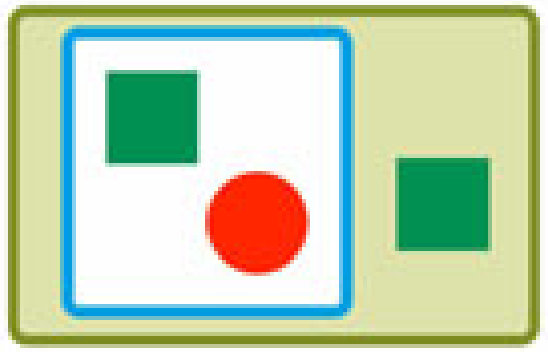
\includegraphics[width=0.06\linewidth]{static/collective2A.png} \ 
\includegraphics[width=0.045\linewidth]{static/collective2B.png}};
%     
%     
%     \node[latent, right=of c2, xshift=1cm] (c1) {$C^1$};
%     \node[const, above=of c1, yshift=0.1cm] (pc1) {$P(c^1|c^2)$};
%     \node[const, above=of pc1, yshift=0.1cm] (nc1) {Col\en{l}ectiv\en{e}\es{o} 1};
%     \node[const, above=of nc1] (fc1) {
\includegraphics[width=0.04\linewidth]{static/collective1A.png} \ 
\includegraphics[width=0.04\linewidth]{static/collective1B.png}};
%     
%     \node[latent, right=of c1, xshift=1cm] (i) {$I$};
%     \node[const, above=of i, yshift=0.1cm] (pi) {$P(i|c^1,c^2)$};
%     \node[const, above=of pi, yshift=0.1cm] (ni) {Individu\en{al}\es{o}};
%     \node[const, above=of ni] (fi) {
\includegraphics[width=0.09\linewidth]{static/individual.png}\ };
%     
%     \node[latent, right=of i, xshift=1cm] (a) { $\A$};
%     \node[const, above=of a, yshift=0.1cm] (pa) {$P(\Aa|i,c^1,c^2)$};
%     \node[const, above=of pa, yshift=0.1cm] (na) {\en{Environment}\es{Ambiente}};
%     \node[const, above=of na] (fa) {\includegraphics[width=0.03\linewidth]{static/water.png}\includegraphics[width=0.04\linewidth]{static/wind.png}\includegraphics[width=0.025\linewidth]{static/fire.png} \ };
%     
%     \edge {c2} {c1};
%     \edge {c1} {i};
%     \edge {i} {a};
%     \path[draw, ->, fill=black,sloped] (c2) edge[bend right,draw=black] node[midway,above,color=black] {} (i);
%     \path[draw, ->, fill=black,sloped] (c2) edge[bend right,draw=black] node[midway,above,color=black] {} (a);
%     \path[draw, ->, fill=black,sloped] (c1) edge[bend right,draw=black] node[midway,above,color=black] {} (a);
%     
%     \plate {aa} {(a)} {}; 
%     }
% \caption{
% \en{Model proposed by Czégel, Zachar and Szathmáry~\cite{czegel2019-bayesianEvolution} to represent multilevel selection. }%
% \es{Modelo propuesto por Czégel, Zachar y Szathmáry~\cite{czegel2019-bayesianEvolution} para representar selección multinivel. }%
% %
% \en{The box represents repetition of the variable. }%
% \es{La caja representa repetición de la variable. }%
% %
% \en{Usually uppercase letters are variable names, and the lowercase letters are specific values. }%
% \es{Usualmente las mayúsculas son nombres de variables, y las minúsculas son sus valores específicos. }%
% }
% 
% \label{fig:czegel_et_el}
% \end{figure}
% %
% \en{The validity of this model is trivial as the product rule always allows the following decomposition, }%
% \es{La validez de este modelo es trivial en tanto la regla del producto siempre permite la siguente descomposición, }%
% %
% \begin{equation}
% P(\Aa,i,c^1,c^2)= P(\Aa|i,c^1,c^2)P(i|c^1,c^2)P(c^1|c^2)P(c^2)
% \end{equation}
% %
% \en{However, the model does not express the causal relationship between the variables. }%
% \es{Sin embargo el modelo no expresa la relación causal entre las variables. }%
% %
% \en{This is evident in all conditional probability distributions. }%
% \es{Esto se constata en todas las distribuciones de probabilidad condicional. }%
% %
% \en{At one extreme, the level 2 collective $C^2$, which is composed of both the level 1 collective and individuals, appears in the model as an independent variable. }%
% \es{En un extremo, el colectivo de nivel 2 $C^2$, que está compuesta tanto por el colectivo de nivel 1 y por los individuos, aparece en el modelo como una variable independiente. }%
% %
% \en{At the other extreme, the environment $\A$, which is usually considered in evolutionary causal models as an independent random variable, appears in this model as dependent on individuals and collectives. }%
% \es{En el otro extremo, el ambiente $\A$, que suele considerarse en los modelos causales evolutivos como una variable aleatoria independiente, aparece en este modelo como dependiente de los individuos y los colectivos. }%
% %
% \en{Conversely, all collectives and individuals appear independent of the environment. }%
% \es{Y a la inversa, todas los colectivos e individuos aparecen independientes del ambiente. }%
% %
% \en{This perhaps explains why the authors avoided specifying conditional probability distributions, and instead provided a pictorial example of the joint probability distribution. }%
% \es{Esto quizás explique porque los autores evitaron especificar las distribuciones de probabilidad condicional, y ofrecieron en cambio un ejemplo pictórico de la distribución de probabilidad conjunta. }%
% 
% \subsection{\en{Basic causal model}\es{Modelo causal básico}}
% 
% \en{The basic causal model we present here serves to introduce the methodology we will use in section \ref{sec:results}, and the conclusion we will draw from it will be of interest later on. }%
% \es{El modelo causal básico que presentamos aquí sirve para introducir la metodología que utilizaremos en la sección \ref{sec:results}, y la conclusión que de él saquemos será de interés más adelante. }%
% % \en{To define conditional probability distributions it is convenient to express the models in causal terms. }%
% % \es{Para definir las distribuciones de probabilidad condicional es conveniente expresar los modelos en términos causales. }%
% \en{This model generalizes the problems analyzed by Lewontin, Yaari and Peters~\cite{lewontin1969-randomlyVaryingEnvironment, peters2019-ergodicityEconomi.s}, and formalizes in probabilistic terms the model proposed by Yaari-Solomon~\cite{yaari2010-cooperationEvolution}. }%
% \es{Este modelo generaliza los problemas analizados por Lewontin-Cohen y Peters~\cite{lewontin1969-randomlyVaryingEnvironment, peters2019-ergodicityEconomics}, y formaliza en términos probabilisticos el modelo propuesto por Yaari-Solomon~\cite{yaari2010-cooperationEvolution}. }% 
% % %
% \en{In them, the binary environmental states depend on a probability $p$. }%
% \es{En ellos, los estados ambientales binarios dependen de un probabilidad $p$. }%
% %
% \begin{equation}
% P(\Aa) = p^{\Aa} (1-p)^{(1-\Aa)}
% \end{equation}
% %
% \en{To define the probability of the strategies, we need a space of alternative strategies, not present in the Lewontin-Cohen and Peters-Amadou models. }%
% \es{Para definir la probabilidad de las estrategia, necesitamos un espacio de estrategias alternativas, no presente en los modelo de Lewontin-Cohen y de Peters-Amadou. }%
% %
% \en{While we are free to propose any set of strategies, we will consider only those that allocate a limited resource $R$ among the binary states of the environment, with $ 0 \leq \Ee \leq R$. }%
% \es{Si bien tenemos la libertad de proponer cualquier conjunto de estrategias, vamos a considerar sólo a aquellas que reparten un recurso limitado $R$ entre los estados binarios del ambiente, con $ 0 \leq \Ee \leq R$. }%
% %
% \en{The strategy proposed by Lewontin-Cohen is $\Ee=1.7$ with $R=2.2$, and the strategy proposed by Peters is $\Ee=1.5$ with $R=2.1$. }%
% \es{La estrategia propuesta por Lewontin-Cohen es $\Ee=1.7$ con $R=2.2$, y la de Peters es $\Ee = 1.5$ con $R=2.1$. }%
% %
% \en{To express all this strategies with a single parameter, we will work only with the family of fitnesses in which $R=1$, $f(\Ee, \Aa)$. }%
% \es{Para expresar las estrategias con un sólo parámetro, vamos a trabajar solamente con la familia de aptitudes en la que $R=1$, $f(\Ee, \Aa)$. }%
% %
% \begin{equation}\label{eq:familia_de_aptitudes}
% f(\Ee, \Aa) = \begin{cases}
%  \Ee & \Aa = 1 \\
%  1-\Ee & \Aa = 0
%   \end{cases}
% \end{equation}
% %
% \en{Now, all strategies lie between 0 and 1: the strategy $\Ee = 1.5/2.1 \approx 0.71$ is the one proposed by Peters, and the strategy $\Ee = 1.7/2.2 \approx 0.77$ is the one proposed by Lewontin-Cohen. }%
% \es{Ahora, todas las estrategias están entre 0 y 1: la estrategia $\Ee = 1.5/2.1 \approx 0.71$ es la propuesta por Peters, y la estrategia $\Ee = 1.7/2.2 \approx 0.77$ es la propuesta por Lewontin-Cohen. }%
% %
% \en{For other ways of defining this same function, see Yaari-Solomon equation 11~\cite{yaari2010-cooperationEvolution}. }%
% \es{Para ver otras formas de definir esta misma función, ver la ecuación 11 de Yaari-Solomon~\cite{yaari2010-cooperationEvolution}. }%
% %
% \en{To define the probability of the strategies given the environment, $p(\Ee|\Aa)$, we need the set of strategies to integrate 1. }%
% \es{Para definir la probabilidad de las estrategias dado el ambiente, $p(\Ee|\Aa)$, necesitamos que el conjunto de estrategias integren 1. }%
% %
% \en{Let's say, for now, that the probability of the strategy is proportional to its fitness, }%
% \es{Digamos, por ahora, que la probabilidad de la estrategia es proporcional a su aptitud, }%
% %
% \begin{equation}\label{eq:probabilidad_propro_aptitud}
% p(\Ee | \Aa) \propto  \Ee^{\Aa}(1-\Ee)^{1-\Aa} = f(\Ee,\Aa)
% \end{equation}
% %
% \en{This allows us to partially define a graphical model with a causal interpretation, }%
% \es{Esto nos permite definir parcialmente un modelo gráfico con una interpretación causal, }%
% %
% \begin{figure}[ht!]
% \centering
% \tikz{
%     \node[latent] (e) {$\A_t$};
%     \node[const, right=of e] (en) {\ $P(\Aa) = p^{\Aa} (1-p)^{(1-\Aa)}$};
%     \node[const, left=of e] (ne) {\en{Environment}\es{Ambiente}: \ \ \ };
%     
%     
%     \node[latent, below=of e] (r) {$\E$};
%     \node[const, right=of r] (rn) {$p(\Ee|\Aa) \propto f(\Ee,\Aa)$};
%     \node[const, left=of r] (nr) {\en{Strategy}\es{Estrategia}: \ \ \ };
%     
%     \edge {e} {r};
%     \plate {ee} {(e)} {$t$}; 
%     }
% \caption{
%  \en{Causal model in which the environment affects individuals. }%
%  \es{Modelo causal en el que el ambiente afecta a los individuos. }%
%  }
% \label{fig:model-lewontin-peters}
% \end{figure}
% %
% \en{in which the environment is an independent random variable and the strategies depends on the observed states of the environment. }%
% \es{en el que el ambiente es una variable aleatoria independiete y las estrategias dependen de los estados observados del ambiente. }%
% %
% \en{Which is the probability $p(\Ee|\Aa)$? }%
% \es{¿Cuál es la probabilidad $p(\Ee|\Aa)$? }%
% 
% \subsection{Sum-product algorithm}
% 
% \en{The \emph{sum-product algorithm} takes advantage of the factoriztion of the joint probability distribution, induced by the causal model, to efficiently apply the rules of probability. }%
% \es{El \emph{sum-product algorithm} aprovecha la factorización de la distribuci\'on de probabilidad conjunta, inducida por el modelo causal, para aplicar eficientemente las reglas de la probabilidad. }%
% %
% \en{It is a way of computing the rules of probability (the sum and product rule) by message passing between probability distributions and their variables. }%
% \es{Es una forma de computar las reglas de la probabilidad (la regla de la suma y el producto) mediante pasaje de mensajes entre las distribuciones de probabilidad y sus variables. }%
% %
% \en{For this purpose, it is convenient to represent the graphical model with a \emph{factor graph}, a bipartite graph with variable nodes (white circles) and function nodes (black squares). }%
% \es{Para ello es conveniente representar el modelo mediante un \emph{factor graph}, un gráfos con nodos variables (círculos blancos), y nodos funciones (cuadrados negros). }%
% %
% \en{The edge between node variables and node functions represents the mathematical relationship ``the variable $v$ is an argument of the function $f$''. }%
% \es{Los ejes entre nodos variables y nodos funciones representan la relaci\'on matem\'atica ``la variable $v$ es argumento de la funci\'on $f$''. }%
% %
% \en{The following factor graph of the graphical model \ref{fig:model-lewontin-peters}. }%
% \es{El siguiente es el factor graph del modelo gráfico \ref{fig:model-lewontin-peters}. }%
% %
% \begin{figure}[H]
% \centering
% \tikz{
% 
%     \node[factor] (fa) {};
%     \node[const, above=of fa] (nfa) {$P(\Aa^t)$};
%     
%     \node[latent, right=of fa] (a) {$\A$};
%     
%     \node[factor, right=of a] (fe) {};
%     \node[const, above=of fe] (nfe) {$p(\Ee|\Aa^t) \propto f(\Ee,\Aa^t)$};
%     
%     \node[latent, right=of fe, xshift=0.3cm] (e) {$\E$};
%     
% 
%      \plate {hola} {(fa)(nfa)(a)(fe)(nfe)} {$\text{Time } t$}; 
% 
%     \edge[-] {fa} {a};
%     \edge[-] {a} {fe};
%     \edge[-] {fe} {e};
%     }
% \caption{
%  \en{Graphical way of representing the factorization of joint distribution induced by the basic causal model (Fig.~\ref{fig:model-lewontin-peters}). }%
%  \es{Forma gráfica de representar la factorizaci\'on de la distribución conjunta inducida por el modelo causal básico (figura~\ref{fig:model-lewontin-peters}). }%
%  %
%  \en{The box represents repetition. }%
%  \es{La caja representa repetición. }%
%  }
% \label{fig:factor_graph}
% \end{figure}
% %
% \en{There are two types of messages: those sent by variable-type nodes to their function-type neighbors ($m_{V \rightarrow F}(v)$) and the ones that function-type nodes send to their variable-type neighbors ($m_{F \rightarrow V}(v)$). }%
% \es{Hay dos tipos de mensajes: los mensajes que envian los nodos variables a sus funciones vecinas ($m_{V \rightarrow F}(v)$); y los mensajes que env\'ian los nodos funciones a sus variables vecinas ($m_{F \rightarrow V}(v)$). }%
% %
% \en{The former partially performs the product rule. }%
% \es{El primero codifica una porci\'on de la regla del producto. }%
% %
% \begin{equation*}\label{eq:m_v_f} \tag{\text{\en{product step}\es{paso del producto}}}
% m_{V \rightarrow F}(v) = \prod_{H}^{\bm{H}} m_{H \rightarrow V}(v)
% \end{equation*}
% %
% \en{where $\bm{H} = n(V) \setminus \{F\}$ represents the set of neighbor nodes to $V$ except $F$. }%
% \es{donde $\bm{H} = n(V) \setminus \{F\}$ representa el conjunto de vecinos del nodo $V$ salvo $F$. }%
% %
% \en{In a brief, the messages sent by the variable-type node $V$ are simply the product of the messages that $V$ receives from the rest of their neighbors $H \in n(V)$ except $F$. }%
% \es{En pocas palabras, los mensajes que env\'ia una variables $V$ es simplemente la multiplicaci\'on de los mensajes que recibi\'o del resto de sus vecinos $H \in n(V)$ salvo $F$. }%
% %
% \en{The other messages sent by the function-type nodes encode a portion of the sum rule. }%
% \es{Los otros mensajes que envían los nodos funciones codifican una parte de la regla de la suma. }%
% %
% \begin{equation*}\label{eq:m_f_v}  \tag{\text{\en{sum step}\es{paso de la suma}}}
% m_{F \rightarrow V}(v) = \sum_{u_1}^{U_1} \dots \sum_{u_n}^{U_n} \Big( F(u_1, \dots, u_n, v) \prod_{U_i}^{\bm{U}} m_{U \rightarrow F}(u_i) \Big)
% \end{equation*}
% %
% \en{where $U_i \in \bm{U} = n(F)\setminus \{V\}$ is the set of all neighbors to $F$ except $V$ of size $n$, $u_i$ is a specific value of the variable $U_i$, $u_i \in U_i$, and $F(u_1, \dots, u_n, v)$ represents the function $F$, evaluated in all its arguments. }%
% \es{donde $U_i \in \bm{U} = n(F)\setminus \{V\}$ es el conjunto de todos los vecinos de $F$ salvo $V$ de tamaño $n$, $u_i$ es un valor específico de la variable $U_i$, $u_i \in U_i$, y $F(u_1, \dots, u_n, v)$ representa la función $F$ evaluada en todos sus argumentos. }%
% %
% \en{In short, the messages sent by the function-type node $F$ to a neighboring variable-type node $V$ is simply the sum (or integration) over $\bm{U}$ of the product of itself and all the messages that receives from the rest of its neighbors $\bm{U}$ except $V$. }%
% \es{En pocas palabras, los mensajes que envía una funci\'on $F$ a una variable vecina $V$ es simplemente la suma (o integraci\'on) sobre $\bm{U}$ del producto de sí mismo con todos los mensajes que recibe del resto de sus vecinos $\bm{U}$ salvo $V$. }%
% %
% \en{Finally, the marginal probability distribution of a variable $V$ is simply the product of the messages that $V$ receives from all its neighbors. }%
% \es{Finalmente, la distribuci\'on de probabilidad marginal de una variable $V$ es simplemente la multiplicaci\'on de los mensajes que $V$ recibe de todos sus vecinos. }%
% %
% \begin{equation*}\label{eq:marginal}  \tag{\text{\en{marginal probability}\es{probabilidad marginal}}}
% P(V=v) = \prod_{H \in n(V)} m_{H \rightarrow V}(v)
% \end{equation*}
% %
% \en{When we observe some variable $u$, we exclude it from the summations, which allows us to compute the marginal probability over two variables, $P(v,u)$. }%
% \es{Cuando observamos alguna variable $u$, la excluímos de las sumatorias, lo que nos permite computar la probabilidad marginal sobre dos variables, $P(v,u)$. }%
% %
% \en{This algorithm encodes the minimum number of steps required to calculate any marginal probability distribution. }%
% \es{Este algoritmo codifica la m\'inima cantidad de pasos que se requieren para calcular cualquier distribuci\'on de probabilidad marginal. }%
% 
% \subsection{\en{Computation of marginal distributions}\es{Computo de distribuciones marginales}}
% 
% \en{As we will later use the sum-product algorithm to solve the extended causal model, we show its use in this basic causal model (figure~\ref{fig:model-lewontin-peters}) to gain some intuition. }%
% \es{Como más adelante utilizaremos el sum-product algorithm para resolver un modelo causal extendido, mostramos su uso en este modelo causal básico (figure~\ref{fig:model-lewontin-peters}) para adquirir un poco de intuición. }%
% %
% \en{Using this procedure we will obtain the marginal distribution of the strategies and a vector of observations $p(\Ee,\vec{\Aa}\,)$, and we will normalize it to obtain the posterior $p(\Ee|\vec{\Aa})$. }%
% \es{Mediante este procedimiento normalizaremos obtendremos la distribución marginal de las estrategias y un vector de observaciones $p(\Ee,\vec{\Aa}\,)$, y la nmormalizaremos para obtener el posterior de las estrategias dado el ambiente $p(\Ee|\vec{\Aa})$. }%
% %
% % \en{Since we want $P(\Ee|\Aa)$ we need the marginals $P(\Ee,\Aa)/P(\Aa)$. }%
% % \es{Como queremos calcular $P(\Ee|\Aa)$ necesitamos las marginales $P(\Ee,\Aa)/P(\Aa)$. }%
% % %
% % \en{Since one of the probability distributions is defined by a proportional term, its marginals will also be proportional. }%
% % \es{Notar que una de las distribuciones de probabilidad está definida de forma proporcional, sus marginales también serán proporcionales. }%
% % %
% \en{To compute $p(\Ee,\Aa)$, we will consider $\Aa=\Aa^*$ observable. }%
% \es{Para computar $p(\Ee,\Aa)$, consideraremos $\Aa=\Aa^*$ observable. }%
% %
% \en{Then, the message from the environment factor $P(\Aa)$ to the environment variable $\A$ is, }%
% \es{Luego, el mensaje del factor del ambiente $P(\Aa)$ a la variable ambiente $\A$ es, }%
% %
% \begin{equation}
% m_{P(\A) \rightarrow \A }(\Aa^*) = P(\Aa^*) = m_{\A \rightarrow p(\E|\A)}(\Aa^*)
% \end{equation}
% %
% \en{which is the same message that the variable $\A$ sends to the strategy factor $p(\E|\A)$. }%
% \es{que es el mismo mensaje que envía la variable $\A$ al factor de estrategias $p(\E|\A)$. }%
% %
% \en{Then, the message sent by the strategies factor $p(\E|\A)$ to the strategies variable $\E$ is, }%
% \es{Luego, el mensaje que envía el factor de estrategias $p(\E|\A)$ a la variable estrategias $\E$ es, }%
% %
% \begin{equation}
% m_{p(\E|\A) \rightarrow \E }(\Ee) \propto P(\Aa^*)f(\Ee,\Aa^*)
% \end{equation}
% %
% \en{Note that we do not integrate the values of the environment because $\Aa^*$ is observable and therefore constant. }%
% \es{Notar que no integramos los valores del ambiente porque $\Aa^*$ es observable y por lo tanto constante. }%
% %
% \en{Then, the marginal of the strategies and a vector of environmental states $\vec{\Aa}$ is, }%
% \es{Luego, la marginal de las estrategias y un vector de estados del ambiente $\vec{\Aa}$ es, }%
% %
% \begin{equation}
% p(\Ee,\vec{\Aa}) \propto \prod_{\Aa}^{\vec{\Aa}} P(\Aa)f(\Ee,\Aa)
% \end{equation}
% %
% % Integrando sobre las estrategia $\E$ obtenemos la marginal de las observaciones,
% % %
% % \begin{align}
% % P(\vec{\Aa}) & \propto \sum_{\Ee}^\E \prod_{\Aa}^{\vec{\Aa}} P(\Aa)f(\Ee,\Aa) \\
% % & = \Big(\prod_{\Aa}^{\vec{\Aa}} P(\Aa) \Big)  \Big( \sum_{\Ee} \prod_{\Aa}^{\vec{\Aa}}f(\Ee,\Aa) \Big) 
% % \end{align}
% % %
% \en{Normalizing it we obtain the posterior, }%
% \es{Normalizando obtenemos el posterior, }%
% %
% \begin{equation}\label{eq:replicator_dynamic_posterior}
% p(\Ee|\vec{\Aa}) = \frac{ \prod_{\Aa}^{\vec{\Aa}}f(\Ee,\Aa)}{\int_{\Ee} \prod_{\Aa}^{\vec{\Aa}}f(\Ee,\Aa)}
% \end{equation}
% %
% % \en{which again has the same structure as the replicator dynamic, this time with an integral instead of a sum because the set of strategies is infinite. }%
% % \es{que nuevamente tiene la misma estructura del replicator dynamic, esta vez con un integral en vez de una suma debido a que el espacio de estrategias es infinito. }%
% %
% %Es decir, el replicator dynamic surgió de considerar el modelo causal en el que el ambiente causa las estrategias y en el que el tamaño de las estrategias depende de la adaptabilidad de esa estrategia al ambiente.
% %
% \en{Then, the posterior belongs to the Beta distribution (note that the denominator of the equation \ref{eq:replicator_dynamic_posterior} is the Beta function or the Euler integral).}
% \es{Luego, el posterior pertenece a la distribución Beta (notar que el denominador de la ecuación \ref{eq:replicator_dynamic_posterior} es la función Beta o la integral de Euler). }%
% %
% \begin{equation}
% P(\Ee|\vec{\Aa}) = \text{Beta}(\texttt{sum}(\vec{\Aa}), \, \texttt{length}(\vec{\Aa}) - \texttt{sum}(\vec{\Aa})) =  \frac{\Ee^{\texttt{sum}(\vec{\Aa})} \cdot (1-\Ee)^{\texttt{length}(\vec{\Aa}) - \texttt{sum}(\vec{\Aa})}}{B(\texttt{sum}(\vec{\Aa}), \, \texttt{length}(\vec{\Aa}) - \texttt{sum}(\vec{\Aa}))} 
% %
% \end{equation}
% %
% \en{with $B(\cdot,\cdot)$ the Beta function. }%
% \es{con $B(\cdot,\cdot)$ la función Beta. }%
% %
% \en{The result of the posterior will indicate the evolutionary stability of the strategies. }%
% \es{El resultado del posterior nos indicará la estabilidad evolutiva de las estrategias. }%
% 
% % Parrafo
% 
% \en{Suppose that the environmental states are generated with probabilities $P(\A = 1) = 0.71$ and $P(\A = 0) = 0.29$. }%
% \es{Supongamos que los estados del ambiente se generan con probabilidades $P(\A = 1) = 0.71$ y $P(\A = 0) = 0.29$. }%
% %
% \en{In Figure~\ref{fig:estrategias_individuales} we show how the posterior of the strategies changes as we add observations to the model. }%
% \es{En la figura~\ref{fig:estrategias_individuales} mostramos cómo cambia el posterior de las estrategias a medida que agregamos observaciones al modelo. }%
% %
% \begin{figure}[H]
%     \centering
%     \begin{subfigure}[b]{0.32\textwidth}
%     \includegraphics[width=\linewidth]{figures/pdf/coin1.pdf}
%     \caption{$T = 1$}
%     \end{subfigure}
%     \begin{subfigure}[b]{0.32\textwidth}
%     \includegraphics[width=\linewidth]{figures/pdf/coin2.pdf}
%     \caption{$T = 10$}
%     \end{subfigure}
%     \begin{subfigure}[b]{0.32\textwidth}
%     \includegraphics[width=\linewidth]{figures/pdf/coin3.pdf}
%     \caption{$T = 10^5$}
%     \end{subfigure}
%     \caption{
%     \en{Posterior probability of strategies as time progresses ($T=1, \, T=10, \, T=10^5$). }%
%     \es{Probabilidad posterior de las estrategias a medida que avanza el tiempo ($T=1, \, T=10, \, T=10^5$). }%
%     }
%     \label{fig:estrategias_individuales}
% \end{figure}
% %
% \en{The evolutionary process selects the strategy that allocates resources in the same proportion as the states of the environment are generated. }%
% \es{El proceso evolutivo selecciona la estrategia que reparte los recursos en la misma proporción que se generan los estados del ambiente. }%
% %
% \en{When the environment generates the states with probability $p=0.71$, then the best adapted strategy is $\Ee = 0.71$. }%
% \es{Cuando el ambientes genera los estados con una probabilidad $p=0.71$, entonces la estrategia mejor adaptada es $\Ee = 0.71$. }%
% % Parrafo
% \en{The selection of individual strategies, now intuitive, will be different and perhaps counter-intuitive when we incorporate the possibility of cooperation and defection into the model. }%
% \es{La selección de estrategias individuales, ahora intuitiva, será diferente y quizás contra-intuitiva cuando incorporemos al modelo la posibilidad de cooperación y deserción. }%
% 
% \section{\en{Results}\es{Resultados}}\label{sec:results}
% 
% % \en{In this section we will analyze whether there is indeed any evolutionary advantage of cooperation and specialization in the presence of defection. }%
% % \es{En esta sección analizaremos si efectivamente existe alguna ventaja evolutiva de la cooperación y la especialización en presencia de deserción. }%
% % %
% \en{To analyze whether there is any evolutionary advantage in favor of cooperation and specialization, in this section we will extend the causal model proposed in the \ref{sec:methodology} section by incorporating unconditionally cooperative behaviors, such as the one presented in the \ref{sec:introduction} section, including defecting behaviors (which receive the benefit of cooperation without contributing to it). }%
% \es{Para analizar si existe alguna ventaja evolutiva a favor de la cooperación y la especialización, en esta sección extenderemos el modelo causal propuesto en la sección \ref{sec:methodology} incorporando comportamientos incondicionalmente cooperativos, como el presentado en la sección \ref{sec:introduction}, incluyendo comportamientos desertores (que reciben el beneficio de la cooperación sin aportar al mismo). }%
% %
% \en{Cooperation in a non-randomly distributed population induces groups formation and therefore a type of group-level selection that acts in parallel to individual-level selection. }%
% \es{La cooperación en poblaciones distribuidas no aleatoriamente induce la formación de grupos y por lo tanto un tipo de selección a nivel grupal que actúa de forma paralela a la selección de nivel individual. }%
% %
% \en{Darwin has already discussed this topic. }
% \es{Darwin ya discutió sobre este tema. }
% %
% \begin{quotation}
% It must not be forgotten that although a high standard of morality gives but a slight or no advantage to each individual (...), an advancement in the standard of morality will certainly given an immense advantage to one tribe over another.
% \end{quotation}
% % \en{This modification alone has a fundamental evolutionary consequence: the formation of groups and thus the emergence of a new evolutionary entity. }%
% % \es{Esta sola modificación tiene una consecuencia evolutiva fundamental: la formación de grupos y por lo tanto la aparición de una nueva entidad evolutiva. }
% %
% \en{In other words, while defecting individuals may have a relative advantage over cooperating individuals, groups may be favored by mutual cooperation. }%
% \es{En otras palabras, si bien los individuos desertores puede tener una ventaja relativa sobre los individuos cooperadores, los grupos pueden verse favorecidos por la mututa cooperación. }%
% %
% \en{The result of both selection processes, known as multilevel selection, is the property of interest. }%
% \es{El resultado de ambos procesos de selección, conocido como selección multinivel, es la propiedad de nuestro interés. }%
% 
% \subsection{\en{Extended causal model}\es{Modelo causal extendido}}
% 
% \en{Individuals are spatially distributed and can interact only with members of the same region. }%
% \es{Los individuos están distribuidos en el espacio y pueden interactuar solamente con los miembros de la misma región. }%
% %
% \en{Suppose we have regions of $N$ individuals in which $n$ are cooperators and $N-n$ defectors. }%
% \es{Supongamos que tenemos regiones de $N$ individuos en el que $n$ son cooperadores y $N-n$ desertores. }%
% %
% \en{Then, there are $N+1$ types of possible regions, from $n=0$ (all defectors) to $n=N$ (all cooperators). }%
% \es{Luego, hay $N+1$ tipos de regiones posibles, desde $n=0$ (todos desertores) hasta $n=N$ (todos cooperadores). }%
% %
% \en{Then, if each individual belongs to a single region we need $M = N(N+1)$ total individuals, $i \in \{1, \dots, M\}$. }%
% \es{Luego, si cada individuo pertenece a una única región necesitamos $M = N(N+1)$ individuos totales, $i \in \{1, \dots, M\}$. }%
% %
% \en{Individuals $i$ are characterized by three attributes: }%
% \es{Los individuos $i$ están caracterizados por tres atributos: }%
% %
% \en{the region to which it belongs, $\texttt{region}(i)=i \ \texttt{div} \ N$; }%
% \es{la región a la que pertenece, $\texttt{region}(i)=i \ \texttt{div} \ N$; }%
% %
% \en{if their social behavior is cooperative, $\texttt{coop}(i) =  i \ \texttt{mod} \ N < \texttt{region}(i)$ (the first $n$ individuals in the region are cooperators and the rest defectors); }%
% \es{si su comportamiento social es cooperador, $\texttt{coop}(i) =  i \ \texttt{mod} \ N < \texttt{region}(i)$ (los primeros $n$ individuos de la región son cooperadores y el resto desertores); }%
% %
% \en{and the strategy $\Ee_i$ they use to allocate resources $f(\Ee,\Aa)$ (equation \ref{eq:familia_de_aptitudes}). }%
% \es{y la estrategia $\Ee_i$ que utilizan para alocar recursos $f(\Ee,\Aa)$ (ecuación~\ref{eq:familia_de_aptitudes}). }%
% %
% \en{By combinatorics, it will be more likely a priori that individuals will inhabit mixed regions. }%
% \es{Por combinatoria, será más probable a priori que los individuos habiten regiones mixtas. }%
% %
% \begin{equation}
% P(i) = \frac{1}{N} \mathcal{B}(\texttt{region}(i)|N,0.5) 
% \end{equation}
% %
% \en{where the binomial distribution $\mathcal{B}$ gives more weight to individuals from mixed regions, the parameter $0.5$ indicates a uniform prior between cooperating and defecting social behaviors, and the factor $\frac{1}{N}$ indicates that all individuals in the same region start with the same initial resources. }%
% \es{donde la distribución binomial $\mathcal{B}$ otorga más peso a los individuos de las regiones mixtas, el parámetro $0.5$ indica un prior uniforme entre los comportamientos sociales cooperador y desertor, y el factor $\frac{1}{N}$ indica que todos los individuos de la misma región empiezan con los mismos recursos iniciales. }%
% %
% \en{As we have seen in the section \ref{sec:methodology}, the probability of the environmental states is, }%
% \es{Como hemos visto en la sección \ref{sec:methodology}, la probabilidad de los estados ambientales es, }%
% %
% \begin{equation}
% P(\Aa) = p^\Aa (1-p)^{1-\Aa}
% \end{equation}
% %
% \en{but now at each time $t$ we have a vector $\vec{\Aa}$, in which the $i-$th element influences the $i-$th individual, }%
% \es{pero ahora en cada tiempo $t$ tenemos un vector $\vec{\Aa}$, en el que el $i-$ésimo elemento influencia al $i-$ésimo individuo, }%
% %
% \begin{equation}
% P(i|\vec{\Aa}) = \frac{\Ee_i^{\Aa_i} (1-\Ee_i)^{1-\Aa_i}}{\sum_j \Ee_j^{\Aa_j} (1-\Ee_j)^{1-\Aa_j}} \propto \Ee_i^{\Aa_i} (1-\Ee_i)^{1-\Aa_i}
% \end{equation}
% %
% \en{Now, however, the agents are also influenced by the resources of the other agents at the previous time, }%
% \es{Ahora sin embargo, los agentes también están influenciados por los recursos del los otros agentes en el tiempo anterior, }%
% %
% \begin{equation}
% P(i^{t+1}|i^t) = 
% \begin{cases}
% 1/N & \texttt{coop}(i^t) \wedge (\texttt{region}(i^{t+1}) = \texttt{region}(i^{t})) \\
% 1 & \neg \texttt{coop}(i^t) \wedge i^{t+1} = i^t \\
% 0 & \texttt{else} \\
% \end{cases}
% \end{equation}
% %
% \en{Cooperating individuals divide the wealth equally with members of the same region, and defecting individuals retain all their wealth. }%
% \es{Los individuos cooperadores dividen la riqueza en partes iguales con los miembros de la misma región, y los individuos desertores se quedan con toda su riqueza. }%
% %
% \en{Finally, the groups are made up of members from each region, $P(g|i)=\mathbb{I}(\texttt{region}(i) = g)$, the indexing function which is $1$ when individuals belong to region $g$ and $0$ otherwise. }%
% \es{Finalmente, los grupos están constituidos por los miembros de cada región, $P(g|i)=\mathbb{I}(\texttt{region}(i) = g)$, la función indiciadora que es $1$ cuando los individuos pertenecen a la región $g$ y $0$ en otro caso. }%
% %
% \begin{figure}[H]
% \centering
%  \begin{subfigure}[b]{0.4\textwidth}    
%  \centering
%  \tikz{
%     
%     \node[obs] (a1) {$\vec{\A}^{\,1}$};
%     \node[obs, right=of a1] (a2) {$\vec{\A}^{\,2}$};
%     
%     \node[latent, below=of a1 ] (i1) {$I^1$};
%     \node[latent, below=of a2 ] (i2) {$I^2$};
%     \node[latent, right=of i2 ] (i3) {$I^3$};
% 
%     \node[latent, below=of i1 ] (c1) {$G^1$};
%     \node[latent, below=of i2 ] (c2) {$G^2$};
%     \node[latent , below=of i3 ] (c3) {$G^3$};
%     
%     \node[invisible, below=of c2, yshift=-0.5cm] (inv) {};
%     
%     
%     \edge {a1} {i1};
%     \edge {a2} {i2};
%     \edge {i1} {i2,c1};
%     \edge {i2} {i3,c2};
%     \edge {i3} {c3};
%     
%     }
%  \caption{\en{Bayesian network}\es{Red bayesiana}}
%  \label{fig:red_bayesiana_multinivel}
%  \end{subfigure}
% \begin{subfigure}[b]{0.58\textwidth}    
%  \centering
%  \tikz{
%     
%     \node[factor] (fa1) {};
%     \node[obs, yshift=0.5cm, below=of fa1] (a1) {$\vec{\A}^{\,1}$};
%     
%     \node[factor, yshift=0.5cm, below=of a1] (fia1) {};
%     
%     \node[latent, yshift=0.5cm, below=of fia1 ] (i1) {$I^1$};
%     
%     \node[factor, xshift=0.3cm, left=of i1 ] (fi0) {};
%     
%     \node[factor, xshift=-0.3cm, right=of i1] (fii1) {};
%     \node[factor, yshift=0.5cm, below=of i1] (fg1) {};
%     \node[latent, yshift=0.5cm, below=of fg1 ] (g1) {$G^1$};
%     
%     \node[latent, xshift=-0.3cm, right=of fii1 ] (i2) {$I^2$};
%     
%     \node[factor, yshift=-0.5cm, above=of i2] (fia2) {};
%     \node[obs, yshift=-0.5cm, above=of fia2] (a2) {$\vec{\A}^{\,1}$};
%     \node[factor, yshift=-0.5cm, above=of a2] (fa2) {};
%     \node[factor, yshift=0.5cm, below=of i2] (fg2) {};
%     \node[latent, yshift=0.5cm, below=of fg2 ] (g2) {$G^2$};
%     
%     \node[factor, xshift=-0.3cm, right=of i2] (fii2) {};
%     
%     \node[latent, xshift=-0.3cm, right=of fii2 ] (i3) {$I^3$};
%     \node[factor, yshift=0.5cm, below=of i3] (fg3) {};
%     \node[latent, yshift=0.5cm, below=of fg3 ] (g3) {$G^3$};
%     
%      \node[const, left=of fa1] (pa) {$P(\vec{\Aa})$};
%      \node[const, left=of fia1] (pea) {$P(i|\vec{\Aa})$};
%      \node[const, left=of fg1] (pg) {$P(g|i)$};
%      \node[const, above=of fii2] (pee) {$P(i^{t+1}|i^t)$};
%      \node[const, left=of fi0] (pa) {$P(i^1)$};
%     
%     
%     \edge[-] {a1} {fa1, fia1};
%     \edge[-] {a2} {fa2, fia2};
%     \edge[-] {i1} {fii1,fg1,fia1,fi0};
%     \edge[-] {i2} {fii1, fii2,fg2,fia2};
%     \edge[-] {i3} {fii2, fg3};
%     \edge[-] {g1} {fg1};
%     \edge[-] {g2} {fg2};
%     \edge[-] {g3} {fg3};
%     }
%  \caption{Factor graph}
%  \label{fig:factor_graph_multinivel}
%  \end{subfigure}
%  \caption{
%  \en{Hierarchical model. }%
%  \es{Modelo jerárquico. }%
%  %
%  \en{Figure~\ref{fig:red_bayesiana_multinivel}: the probabilistic dependencies arising from the multilevel causal model. }%
%  \es{Figura~\ref{fig:red_bayesiana_multinivel}: las dependencias probabilísiticas que surge del modelo causal multinivel. }%
%  %
%  \en{Figure~\ref{fig:factor_graph_multinivel}: the factor graph induced by the Bayesian network, which will be used to apply the sum-product algorithm. }%
%  \es{Figura~\ref{fig:factor_graph_multinivel}: el grafo de factores inducido por la red bayesiana, que será utilizado para aplicar el algoritmo suma-producto. }%
%  %
%  \en{The gray variables are observed. }%
%  \es{Las variables en gris se consideran observables. }%
%  }
% \label{fig:multilevel_model}
% \end{figure}
% %
% \en{In short, at each time $t$ the environment influences individuals, and individuals influence the groups of their own time and the individuals of time $t+1$. }%
% \es{En resumen, en cada tiempo $t$ el ambiente influencia a los individuos, y los individuos influencian a los grupos de su propio tiempo y a los individuos del tiempo $t+1$. }%
% %
% \en{This model has $3$ hyperparameters: the vector of strategies $\vec{\Ee}$, the probability of the environment $p$, and the size of the groups $N$. }%
% \es{Este modelo tiene $3$ hiperparámetros: el vector de estrategias $\vec{\Ee}$, la probabilidad del ambiente $p$, y el tamaño de los grupos $N$. }%
% %
% %Este modelo se puede simplificar levemente, usando una única variable de grupo que dependa de la última variable individuo, gracias a que la margnial de los grupos es la misma en cualquier tiempo $t$.
% 
% % Parrafo
% 
% \en{The evolutionary problem we are interested in is the selection of cooperative individuals given the environment within each group (level 1), $P(\texttt{coop}(i^T)|\vec{\Aa}^{\,1}, \dots, \vec{\Aa}^{\,T-1}, g)$, the selection of groups given the environment (level 2), $P(g^T|\vec{\Aa}^{\,1}, \dots, \vec{\Aa}^{\,T-1})$,  and selection of cooperative individuals given the environment for all groups (multilevel), $P(\texttt{coop}(i^T)|\vec{\Aa}^{\,1}, \dots, \vec{\Aa}^{\,T-1})$. }%
% \es{El problema evolutivo que nos interesa es la selección de los individuos cooperadores dado el ambiente dentro de cada grupo (nivel 1), $P(\texttt{coop}(i^T)|\vec{\Aa}^{\,1}, \dots, \vec{\Aa}^{\,T-1}, g)$, la selección de los grupos dado el ambiente (nivel 2), $P(g^T|\vec{\Aa}^{\,1}, \dots, \vec{\Aa}^{\,T-1})$, y la selección de los individuos cooperadores dado el ambiente integrando todos los grupos (multinivel), $P(\texttt{coop}(i^T)|\vec{\Aa}^{\,1}, \dots, \vec{\Aa}^{\,T-1})$. }%
% %
% \en{The multilevel selection is obtained by integrating the product of level 1 and 2 selections, }%
% \es{La selección multinivel se obtiene integrando el producto de las selecciones de nivel 1 y 2, }%
% %
% \begin{equation}\label{eq:posterior_multinivel}
% \underbrace{P(\texttt{coop}(i^T)|\vec{\Aa}^{\,1}, \dots, \vec{\Aa}^{\,T-1})}_{\text{\en{Multilevel selection}\es{Selección multinivel}}} = \sum_{g=0}^N \underbrace{P(\texttt{coop}(i^T)|\vec{\Aa}^{\,1}, \dots, \vec{\Aa}^{\,T-1}, g)}_{\text{\en{Level 1 selection}\es{Selección de nivel 1}}} \cdot \underbrace{P(g^T|\vec{\Aa}^{\,1}, \dots, \vec{\Aa}^{\,T-1})}_{\text{\en{Level 2 selection}\es{Selección de nivel 2}}}
% \end{equation}
% %
% \en{where the posterior of level 1 selection is obtained by integrating the probability of all cooperating individuals that are part of the group $g$, }%
% \es{donde el posterior de la selección de nivel 1 se obtiene integrando la probabilidad de todos los individuos cooperadores que forman parte del grupo $g$, }%
% %
% \begin{equation}\label{eq:posterior_nivel_1}
% \begin{split}
% P(\texttt{coop}(i^T)|\vec{\Aa}^{\,1}, \dots, \vec{\Aa}^{\,T-1}, g) &= \sum_{j=1}^M P(I^T=j|\vec{\Aa}^{\,1}, \dots, \vec{\Aa}^{\,T-1}, g)\mathbb{I}(\texttt{coop}(j))
% \end{split}
% \end{equation}
% %
% \en{An alternative way to compute the multilevel selection marginal (Eq.~\ref{eq:posterior_multinivel}) is by integrating the probability of all cooperating individuals given the environments }%
% \es{Una forma alternativa de calcular la marginal de la selección multinivel (Eq.~\ref{eq:posterior_multinivel}) es integrando la probabilidad de los individuos cooperadores dado los ambientes }%
% %
% \begin{equation}\label{eq:posterior_multinivel_alternativa}
% \begin{split}
% P(\texttt{coop}(i^T),\vec{\Aa}^{\,1}, \dots, \vec{\Aa}^{\,T-1}) &= \sum_{j=1}^M P(I^T=j,\vec{\Aa}^{\,1}, \dots, \vec{\Aa}^{\,T-1})\mathbb{I}(\texttt{coop}(j))
% \end{split}
% \end{equation}
% %
% \en{where the probability of individuals, when the environmental states $\vec{\Aa}^{\,t}$ are observed, is }%
% \es{donde la probabilidad de los individuos cuando tenemos como observable todos los ambientes $\vec{\Aa}^{\,t}$ es, }%
% %
% \begin{equation}
% P(i^{T},\vec{\Aa}^{\,1}, \dots, \vec{\Aa}^{\,T-1}) = m_{P(I^{T}|I^{T-1}) \rightarrow I^T}(i^T)
% \end{equation}
% %
% \en{This message is recursively defined. }%
% \es{Este mensaje está definido recursivamente. }%
% %
% \begin{equation}\label{eq:m_pii_i}
% \begin{split}
% m_{P(I^{t+1}|I^{t}) \rightarrow I^{t+1} }(i^{t+1}) & = \sum_{i^t} P(i^{t+1}|i^t) \, P(\vec{\Aa}^{\,t}) \, P(i^t|\vec{\Aa}^{\,t}) \,  m_{P(I^t|I^{t-1}) \rightarrow I^t }(i^t) 
% \end{split}
% \end{equation}
% %
% %
% %
% % En la introducción hemos derivado la tasa de crecimiento de esta marginal para los grupos enteramente desertoras y solo hemos presentado un resultado numérico para el grupo enteramente cooperador.
% % %
% % En la siguiente sección resolveremos analíticamente el posterior de la selección de grupos y multinivel y verificaremos la hipótesis de Ole Peters de la ventaja evolutiva de la cooperación.
% % %
% % Y la sección \ref{sec:especialization}, haremos uso de los resultado análitico para demostrar la ventaja evolutiva de la especilización, rechazando la hipótesis de Ole Peters de que la especialización es un mecanismo implausible para poblaciones chicas.
% % 
% % 
% % En esta subsección resolveremos la marginal que necesitamos para computar el posterior de la la selección de nivel 1, de nivel 2 y multinivel,
% % %
% % \begin{equation}
% % \begin{split}
% % P(I^{T+1}=k, \vec{\Aa}^{\,1}, \dots, \vec{\Aa}^{\,T}) & = m_{P(I^{T+1}|I^{T}) \rightarrow I^{T+1} }(k)
% % \end{split}
% % \end{equation}
% % %
% % donde el mensaje está definido recursivamente en la ecuación~\ref{eq:m_pii_i}.
% %
% %
% \en{In all cases, the marginal is equal to the posterior times the probability of the observed environment, }%
% \es{En todos los casos, la marginal es igual al posterior por la probabilidad del ambiente observado, }%
% %
% \begin{equation}
% \begin{split}
% P(I^{T+1}=k, \vec{\Aa}^{\,1}, \dots, \vec{\Aa}^{\,T}) & = P(k| \vec{\Aa}^{\,1}, \dots, \vec{\Aa}^{\,T}) \prod_{t=1}^T P(\vec{\Aa}^{\,t})
% \end{split}
% \end{equation}
% %
% \en{where}\es{donde} (\en{all steps are described in detail in the appendix}
% \es{en el anexo resolvemos todos los pasos detalladamente})
% %
% \begin{equation}
% P(k| \vec{\Aa}^{\,1}, \dots, \vec{\Aa}^T) = 
% \begin{cases}
% P(k)\prod_{t=1}^{T} P(k|\vec{\Aa}^{\,t}) &  r=0  \\
% P(k)\prod_{t=1}^{T} \sum_j^{\texttt{\en{partners}\es{socios}}(r)} \frac{1}{N} P(j|\vec{\Aa}^{\,t}) & r  = N  \\
% \Big(P(k)\prod_{t=1}^{T} P(k|\vec{\Aa}^{\,t}) \Big) + \Big(\sum_{t=1}^{T} P(c|\wedge_{q=1}^t\vec{\Aa}^{\,q})  \prod_{q=t+1}^T P(k|\vec{\Aa}^{\,q}) \Big) & 0 < r < N  
% \end{cases}
% \end{equation}
% %
% \en{where $r = \texttt{region}(k)$ is the region to which individual $k$ belongs, $\texttt{partners}(r)$ is the set of cooperating individuals in region $r$, and $c$ is a cooperative individual belonging to that specific region, $c \in \texttt{partners}(r)$. }%s
% \es{donde $r = \texttt{region}(k)$ es la región a la que pertenece el individuo $k$, $\texttt{\en{partners}\es{socios}}(r)$ es el conjunto de individuos cooperadores de la región $r$, y $c$ es un individuo cooperador de esa región, $c \in \texttt{\en{partners}\es{socios}}(r)$. }%
% 
% \subsection{\en{The multiplicative nature of evolutionary and probability theories}\es{La naturaleza multiplicativa de las teorías de la evolución y la probabilidad}}
% 
% \en{Even if our causal model does not assume any kind of process to update resources, the result of the inference is proportional to the resources obtained through a multiplicative process. }%
% \es{Incluso si nuestro modelo causal no presupone ningún tipo de proceso para actualizar los recursos, el resultado de la inferencia es proporcional a los recursos obtenidos a través de un proceso multiplicativo. }%
% % \en{The proposed causal model does not require assuming that the resource updating process is multiplicative, as proposed by Ole Peters for his game. }%
% % \es{El modelo causal propuesto no requiere suponer que el proceso de actualización de los recursos sea multiplicativo, como propone Ole Peters para su juego. }%
% % %
% \en{All the assumptions of our model are made explicit in the Bayesian network in Figure~\ref{fig:multilevel_model}. }
% \es{Todos los supuestos de nuestro modelo se encuentran explicitados en la red bayesiana de la figura~\ref{fig:multilevel_model}. }%
% %
% \en{Individuals are affected just by the environment and by the social behaviors of cooperation and defection of their context. }%
% \es{Los individuos se ven afectados solamente por el ambiente y por los comportamientos sociales de cooperación y deserción de su contexto. }%
% %
% \en{However, our probabilistic causal model and the multiplicative process discussed in the introduction are equivalent. }%
% \es{Sin embargo, nuestro modelo causal probabilístico y el proceso multiplicativo analizado en la introducción son equivalentes. }%
% %  
% % % Parrafo
% % 
% % \en{Without the need to presuppose a multiplicative process, the posteriors of individuals in our causal model are proportional to the trajectory of resources arising from the game proposed by Ole Peters. }%
% % \es{Sin necesidad de presuponer un proceso multiplicativo, los posteriors de los individuos en nuestro modelo causal son proporcionales a la trayectoria de los recursos que surgen del juego propuesto por Ole Peters. }%
% %
% \en{The posterior of individuals from the entirely defecting region is, }%
% \es{El posterior de los individuos de la región enteramente desertora es, }%
% %
% \begin{equation}
% \begin{split}
% P(i^{T+1} | \vec{\Aa}^{\,1}, \dots, \vec{\Aa}^{\,T}) & \overset{r=0}{=}  P(i^{T+1})  \prod_{t=1}^{T} P(i^{T+1}|\vec{\Aa}^{\,t}) \\
% & \propto P(i^{T+1}) \prod_{t=1}^{T} \Ee_k^{\Aa_k} (1-\Ee_k)^{1-\Aa_k}   \propto P(i^{T+1}) \prod_{t=1}^{T} R f(\Ee_i,\Aa_{i}^{t})
% \end{split}
% \end{equation}
% %
% \en{where $r = \texttt{region}(i^{T+1}) = 0$ denotes the region without cooperators, $f$ is the fitness function that we define in the equation \ref{eq:familia_de_aptitudes}. }%
% \es{donde $r = \texttt{region}(i^{T+1}) = 0$ indica la región sin cooperadores, $f$ es la familia de aptitudes que definimos en la ecuación \ref{eq:familia_de_aptitudes}. }%
% %
% \en{The first proportional is valid because of the normalization constant of the probability distribution $P(i^t|\vec{\Aa}^{\,t})$. }%
% \es{El primer proporcional vale por constante de normalización de la distribución de probabilidad $ P(i^t|\vec{\Aa}^{\,t})$. }%
% %
% \en{And the second proportional simply includes the factor $R$, so that the fitness function matches the one proposed by Lewontin-Cohen, when $R=2.2$, or the one proposed by Peters, when $R=2.1$. }%
% \es{Y el segundo proporcional simplemente incluye el factor $R$ para que la función de aptitudes coincida con la prouesta por Lewontin-Cohen, cuando $R=2.2$, o la propuesta por Peters, $R=2.1$. }%
% %
% \en{When the prior $P(i^{T+1})$ represents the initial resources $\omega(0)$, then the posterior of the individual defectors in entirely defecting groups is proportional to the growth of the individual resources studied in the introduction section. }%
% \es{Si consideramos que el prior $P(i^{T+1})$ representa los recursos inciales $\omega(0)$, luego el posterior de los individuos desertores en grupos enteramenete desertoras es proporcional al crecimiento de los recursos individuales estudiada en la introducción. }%
% 
% % Parrafo
% 
% \en{The same is true for the posteriors of cooperating individuals. }%
% \es{Lo mismo ocurre con los posteriors de los individuos cooperadores. }%
% %
% \en{First, the message sent by the individual variables to the social factor is proportional to the second node of the cooperative protocol (figure~\ref{fig:protocolo}), in which the previous resources $\omega_i(t)$ are updated by the product of the fitness function. }%
% \es{Primero, el mensaje que envían las variables individuos al factor social es proprocional al segundo nodo de del protocolo cooperativo (figura~\ref{fig:protocolo}), en el que los recursos previos $\omega_i(t)$ mediante el producto de la función de fitness. }%
% %
% \begin{equation}
% \begin{split}
% m_{I^t \rightarrow P(I^{t+1}|I^t)}(i^t) & = m_{P(I^t|\vec{\A}^{\,t}) \rightarrow I^t}(i^t) \, m_{P(I^t|I^{t-1}) \rightarrow I^t }(i^t) \\
% & = P(i^t| \vec{\Aa}^{\,t}) \, P(i^t, \vec{\Aa}^{\,t}, \dots, \vec{\Aa}^{\,t}) \\
% & \propto R\,f(\,\Ee_i,\Aa_{i}^{t}) \omega(t-1)
% \end{split}
% \end{equation}
% %
% %donde la marginal $P(i^t, \vec{\Aa}^{\,t}, \dots, \vec{\Aa}^{\,t})$ es proporcional al posterior $P(i^t| \vec{\Aa}^{\,t}, \dots, \vec{\Aa}^{\,t})$.
% %
% \en{Again, the proportionality holds by construction of the probability distribution $P(i^t|\vec{\Aa}^{\,t})$. }%
% \es{Nuevamente, la prorporcionalidad vale por construcción de la distribución de probabilidad $P(i^t|\vec{\Aa}^{\,t})$. }%
% %
% \en{And the message that the social factor sends to the individual variable of the following time is proprotional to the individual resources after pooling and sharing, }%
% \es{Y el mensaje que envía el factor social a la variable individuo del siguiente tiempo es proprocional a los recursos individuales luego de la redistribución del fondo común, }%
% %
% \begin{equation}
% \begin{split}
% m_{P(I^{t+1}|I^{t}) \rightarrow I^{t+1} }(i^{t+1}) & = \sum_{i^t} P(i^{t+1}|i^t) \, P(\vec{\Aa}^{\,t}) \, P(i^t|\vec{\Aa}^{\,t}) \,  m_{P(I^t|I^{t-1}) \rightarrow I^t }(i^t) \\
% %& \propto \sum_{i^t} P(i^{t+1}|i^t) \, P(i^t|\vec{\Aa}^{\,t}) \,  \text{Prior}(i^t) \\
% = P(I^{t+1}, \vec{\Aa}^{\,1} , \dots, \vec{\Aa}^{\,T} ) & \propto \sum_{i^t} P(i^{t+1}|i^t) \, f_{\Ee_i}(\Aa_{i}^{t}) \omega_i(t)  = \omega_i(t+1)
% \end{split}
% \end{equation}
% %
% \en{where $P(i^{t+1}|i^t) = \frac{1}{N}$ when individuals belong to the same region $\texttt{region}(i^{t+1}) = \texttt{region}(i^{t})$. }%
% \es{donde $P(i^{t+1}|i^t) = \frac{1}{N}$ cuando los individuos pertenecen a la misma región $\texttt{region}(i^{t+1}) = \texttt{region}(i^{t})$. }%
% %
% \en{This message generalizes the last node of the cooperative protocol (figure~\ref{fig:protocolo}). }%
% \es{Este mensaje generaliza el último nodo del protocolo cooperativo (figura~\ref{fig:protocolo}). }%
% 
% % Parrafo
% 
% \en{In the introduction we have not analyzed the resource trajectory of defectors in cooperative groups, but in general, the posterior of individuals is no more than the proportion of resources they manage. }%
% \es{En la introducción no hemos analizado la trayectoria de los recursos de los desertores en grupos cooperativos, pero en general, el posterior de los individuos no es más que la proporción de recursos que maneja. }%
% %
% \begin{equation}
% P(k| \vec{\Aa}^{\,1}, \dots,  \vec{\Aa}^{\,T}) = \frac{\omega_k(T)}{\sum_j \omega_j(T)}
% \end{equation}
% %
% \en{The proportionality between the posterior probability of individuals and the trajectories of resources studied in the introduction section allows us to work with both expressions interchangeably. }%
% \es{La proporcionalidad entre la probabilidad a posteriori de los individuos y las trayectorias de los recursos estudiada en la instroducción nos permite trabajar indistintamanete con una u otra expresión. }%
% 
% % Parrafo
% 
% \en{The multiplicative updating of the probabilities of individuals, which arises naturally from applying the rules of probability to the causal model, is in line with the long-established idea in evolutionary theory that the growth of lineages follow multiplicative processes~\cite{dempster1955-geometricMean, denBoer1968-spreadingRisk}. }%
% \es{La actualización multiplicativa de las probabilidades de los individuos, que surge naturalmente de aplicar las reglas de la probabilidad al modelo causal, está en línea con la idea largamente establecida en la teoría de la evolución de que el crecimiento de los linajes siguen procesos multiplicativos~\cite{dempster1955-geometricMean, denBoer1968-spreadingRisk}. }% 
% %
% \en{This coincidence is an additional support to the hypothesis of isomorphism between evolutionary and probability theories, previously identified between their fundamental equations: the Bayes theorem and the replicator dynamic~\cite{harper2009-replicatorAsInference,shalizi2009-replicatorAsInference}. }%
% \es{Esta coincidecia es un apoyo adicional a la hipótesis de isomorfimo entre las teorías de la evolutivas y probabilisticas, previamente identificado entre sus ecuaciones fundamentales: el teorema de bayes y el replicator dynamic~\cite{harper2009-replicatorAsInference,shalizi2009-replicatorAsInference}. }%
% 
% \subsection{\en{Commons dilemma}\es{Dilema de los bienes comunes}}
% 
% \en{In the last few decades evolutionary biology has begun to adopt the analogy of the ``tragedy of the commons''~\cite{rankin2007-tragedyCommonsBiology}. }%
% \es{En las últimas décadas la biología evolutiva ha comenzado a adoptar la analogía de la ``tragedia de los comunes''~\cite{rankin2007-tragedyCommonsBiology}. }%
% %
% \en{This concept contains the idea that the commons has a payoff structure isomorphic to the N-player prisoner's dilemma~\cite{hardin1971-collectiveAsPrisionerDilema}. }%
% \es{Este concepto contiene la idea de que los bienes comunes tienen una estructura de pagos isomorfa al dilema del prisionero de N jugadores~\cite{hardin1971-collectiveAsPrisionerDilema}. }%
% %
% \en{In a two-player prisoner's dilemma, cooperating implies a cost $c$ for the other person to receive a benefit $b$, with $b > c$, and defecting means refusing to cooperate and carries no cost. }%
% \es{En un dilema del prisionero de dos jugadores, cooperar implica un coste $c$ para que la otra persona reciba un beneficio b, con $b > c$, y desertar significa negarse a cooperar y no conlleva ningún coste. }% 
% %
% \begin{equation}
%   \bordermatrix{ & C & D \cr
%       C & b-c & -c \cr
%       D & b & 0 } 
% \end{equation}
% %
% \en{Players gain more if they opt for mutual cooperation than for mutual defection, since $b - c > 0$. }%
% \es{Los jugadores ganan más si optan por la cooperación mutua que por la deserción mutua, ya que $b - c > 0$. }%
% %
% \en{However, regardless of what the other player does, it is better not to cooperate: if my partner defects, it is better for me to defect than to cooperate, since $0 > -c$; if my partner cooperates, it is still better for me to defect than to cooperate, since $b > b - c$. }%
% \es{Sin embargo, independientemente de lo que haga el otro jugador, es mejor no cooperar: si mi compañero deserta, es mejor para mí desertar que cooperar, ya que $0 > -c$; si mi compañero coopera, sigue siendo mejor para mí desertar que cooperar, ya que $b > b - c$. }%
% %
% \en{This creates a dilemma: although mutual cooperation is a preferable outcome, no individual has the incentive to cooperate. }%
% \es{De ahí el dilema: aunque la cooperación mutua es un resultado preferible, ningún individuo tiene el incentivo de cooperar. }%
% 
% % Parrafo
% 
% %En vez de utilizar una matriz de pagos del dilema del prisionero para representar un proceso de bienes comunes, en nuestro trabajo definimos el proceso de bienes comunes a partir del cual podemos derivar la matriz de pagos asociada.
% %
% \en{If our causal model had a payoff structure isomorphic to the prisoner's dilemma, then defectors would have a higher growth rate than cooperators. }%
% \es{Si nuestro modelo causal tuviera una estrucutra de pagos isomorfa al dilema del prisioner, entonces los desertores tendrían una tasa de crecimiento mayor a lo cooperadores. }%
% %
% \en{However, the first defector from an entirely cooperative group obtains a lower growth rate than before defecting. }%
% \es{Sin embargo, el primer desertor de un grupo enteramente cooperadora obtiene una tasa de crecimiento menor a la que tenía antes de desertar. }% 
% %
% \en{In the figure~\ref{fig:ergodicity_desertion} we can observe the trajectories of the resources, equivalent to the proportional posterior (see previous section), of the individuals that are in a group of size 100. }%
% \es{En la figura~\ref{fig:ergodicity_desertion} podemos observar las trayectoria de los recursos, equivalente el posterior proporcional (ver sección anterior), de los individuos que están en un grupos de tamaño 100. }%
% %
% \begin{figure}[ht!]
%     \centering
%     \begin{subfigure}[b]{0.5\textwidth}
%     \includegraphics[width=\linewidth]{figures/pdf/ergodicity_desertion.pdf}
%     \end{subfigure}
%     \caption{
%     \en{The colors represent groups of size 100 with 0, 1 and 2 defectors. }%
%     \es{Los colores representan los grupos de tamaño 100 con 0, 1 y 2 desertores. }%
%     %
%     \en{The curves of the individual defectors are those at the top of each of the groups. }%
%     \es{Las curvas de los individuos desertores son las que están arriba en cada uno de los grupos. }%
%     }
%     \label{fig:ergodicity_desertion}
% \end{figure}
% %
% \en{The resources of the first individual defector (blue group with 1 defector), is below the resources of the individuals in the fully cooperative group (green group with 0 defectors). }%
% \es{Los recursos del primer individuo desertor (grupo azul con 1 desertor), está por debajo de los recursos de los individuos del grupo enteramente cooperador (grupo verde con 0 desertores). }%
% %
% \en{The reduction in resources occurs even for the second individual who changes from cooperative to a defective behavior. }%
% \es{La reducción de recursos le ocurre incluso al segundo individuo que cambia de comportamiento cooperador a desertor. }%
% 
% % Parrafo
% 
% \en{Defecting, instead of increasing the growth rate of the defective individuals, reduces it. }%
% \es{Desertar, en vez de aumentar la tasa de crecimiento de los individuos desertores, la reduce. }%
% %
% \en{In other words, the commons does not have the structure of the prisoner's dilemma, as is usually claimed in the literature. }%
% \es{Es decir, los bienes comunes no tiene la estructura del dilema del prisionero como habitualmente se afirma en la literatura. }%
% %
% \en{Let us calculate the payoff matrix arising from the cooperative causal model. }%
% \es{Calculemos la matriz de pagos que surge del modelo causal cooperativo. }%
% %
% \en{We want to estimate the temporal growth rate of the posteriors, }%
% \es{Queremos estimar la tasa de crecimiento temporal de los posteriors, }%
% %
% \begin{equation}
% \frac{P(k|\vec{\Aa}^{\,1}, \dots , \vec{\Aa}^{\,T})}{P(k)} \approx g(k|\vec{\Ee},p,N)^T
% \end{equation}
% %
% \en{where the approximation is an equality when time tends to infinity, $\lim_{T \rightarrow \infty}$. }%
% \es{donde la aproximación es una igualdad cuando el tiempo tiende a infinito, $\lim_{T \rightarrow \infty}$. }%
% %
% \en{The growth rate depends on the hyperparameters of the model, $\vec{\Ee}$, $p$ and $N$. }%
% \es{La tasa de crecimiento depende de los hyperparámtros del modelo, $\vec{\Ee}$, $p$ y $N$. }%
% %
% \en{Here we will only consider models in which all individuals have the same strategy $\Ee$. }%
% \es{Aquí vamos a considerar únicamente los modelos en el que todos los individuos tienen la misma estrategia $\Ee$. }%
% %
% \en{We will solve this problem by cases, depending on whether the behavior is cooperative, $g_C$, or defective, $g_D$, for different social contexts $g_{[\cdot]}^n(k|\cdot)$, where $n$ represents the number of cooperators with which the individual $k$ interacts (excluding $k$). }%
% \es{Resolveremos este problema por casos, según el comportamiento sea cooperativo, $g_C$, o desertivos, $g_D$, para diferente contextos sociales $g_{[\cdot]}^n(k|\cdot)$, donde $n$ representa la cantidad de cooperadores con lo que interactúa el individuo $k$ (excluyendo a $k$). }%
% % 
% \en{The growth rate of mutual defection is, }%
% \es{La tasa de crecimiento de la deserción mutua es, }%
% %
% \begin{equation}
% \begin{split}
% \lim_{T \rightarrow \infty} g_D^0(k|\Ee,p,N)^T &= \prod_{t=1}^T P(k|\vec{\Aa}^{\,T+1}) \propto \prod_{t=1}^T \Ee^{\Aa^t_k} (1-\Ee)^{1-\Aa^t_k} \\
% \lim_{T \rightarrow \infty} g_D^0(k|\Ee,p,N) &\propto \Big( \prod_{t=1}^T \Ee^{\Aa^t_k} (1-\Ee)^{1-\Aa^t_k} \Big) ^{1/T} = \Ee^{p} (1-\Ee) ^{1-p}
% \end{split}
% \end{equation}
% %
% \en{which is independent of the size $N$. }%
% \es{que es independiete del tamaño $N$. }%
% %
% \en{The proportional is valid because of the normalization constant of the probability distribution $P(i^t|\vec{\Aa}^{\,t})$. }%
% \es{El proporcional vale por constante de normalización de la distribución de probabilidad $ P(i^t|\vec{\Aa}^{\,t})$. }%
% %
% \en{The growth rate of a strategy $\Ee= 0.71 \approx 1.5/2.1$ in an environment with $p=0.5$ is $ 0.71^{1/2}\cdot0.29^{1/2} \approx 0.452$. }%
% \es{La tasa de crecimiento de un estrategia $\Ee= 0.71 \approx 1.5/2.1$ en una ambiente con $p=0.5$ es $ 0.71^{1/2}\cdot0.29^{1/2} \approx 0.452$. }%
% 
% % Parrafo
% 
% \en{The growth rate of the cooperators can also be computed using the geometic average, }
% \es{La tasa de crecimiento de los cooperadores también la podemos calcular utilizando la media geomética, }%
% %
% \begin{equation}
% \begin{split}
% \lim_{T \rightarrow \infty} g_C^n(k|\Ee,p,N)^T &= \prod_{t=1}^{T} \sum_j^{\texttt{\en{partners}\es{socios}}(k)} \frac{1}{N} P(j|\vec{\Aa}^{\,t}) \propto \prod_{t=1}^{T}  \sum_j^{\texttt{\en{partners}\es{socios}}(k)} \frac{1}{N} \Ee^{\Aa^t_j} (1-\Ee)^{1-\Aa^t_j} \\
% \lim_{T \rightarrow \infty} g_C^n(k|\Ee,p,N) & \propto \Big( \prod_{t=1}^{T}  \sum_j^{\texttt{\en{partners}\es{socios}}(k)} \frac{1}{N} \Ee^{\Aa^t_j} (1-\Ee)^{1-\Aa^t_j} \Big)^{1/T} = \prod_{x=0}^{n+1} \Big(\frac{x}{N} \Ee + \frac{n+1-x}{N}(1-\Ee)\Big)^{\mathcal{B}(x|n+1,p)}
% \end{split}
% \end{equation}
% %
% \en{where $x$ represents the number of successes within the cooperating group, and $\mathcal{B}(x|n+1,p)$ is the binomial probability of obtaining $x$ successes in a sample of size $n+1$. }%
% \es{donde $x$ representa la cantidad de éxitos dentro del grupo cooperador, y $\mathcal{B}(x|n+1,p)$ es la probabilidad binomial de obtener $x$ éxitos en una muestra de tamaño $n+1$. }%
% %
% % %
% % \begin{equation}
% % f_C(\Ee,\vec{\Aa}\,) =
% % \begin{cases}
% % (1-\Ee) & \text{ si } \texttt{sum}(\vec{\Aa}\,) = 0 \\
% % \frac{1}{3} \Ee + \frac{2}{3} (1-\Ee)  & \text{ si } \texttt{sum}(\vec{\Aa}\,) = 1 \\
% % \frac{2}{3} \Ee + \frac{1}{3} (1-\Ee)    & \text{ si } \texttt{sum}(\vec{\Aa}\,) = 2 \\
% % \Ee & \text{ si } \texttt{sum}(\vec{\Aa}\,) = 3
% % \end{cases}
% % \end{equation}
% % %
% % Y en general, 
% % \begin{equation}\label{eq:fitness_cooperador}
% % f_{C}(\Ee, \vec{\Aa}\,,N) = \frac{\texttt{sum}(\vec{\Aa}\,)}{N} \Ee + \frac{N-\texttt{sum}(\vec{\Aa}\,)}{N}(1-\Ee)
% % \end{equation}
% % %
% % \en{where $f_C(\Ee, \vec{\Aa}\,,N) \sim \text{Binomial}(\texttt{sum}(\vec{\Aa}\,)|N,p)$, with $p$ the probability of the environment. }%
% % \es{donde $f_C(\Ee, \vec{\Aa}\,,N) \sim \text{Binomial}(\texttt{sum}(\vec{\Aa}\,)|N,p)$, con $p$ la probabilidad del ambiente. }%
% % %
% % \en{Then, the growth rate of the mutual cooperation can be computed using the geometic average~\ref{eq:geometric_mean}, }
% % \es{Luego, la tasa de crecimiento de la mutua cooperación la podemos calcular utilizando la media geomética~\ref{eq:geometric_mean}, }%
% % %
% % \begin{equation}
% % g_{C}(\Ee,N) = \prod_{x=0}^N \Big(\frac{x}{N} \Ee + \frac{N-x}{N}(1-\Ee)\Big)^{\text{Binomial}(x|N,p)}
% % \end{equation}
% %
% \en{Then, the cooperative growth rate in a group of size 2 are $g_C^2(k|\Ee=0.71,p=0.5,N=2) \propto 0.71^{1/4}\cdot 0.5^{1/2} \cdot 0.29^{1/4} \approx 0.475$ and $g_C^1(k|\Ee=0.71,p=0.5,N=2) \propto (\frac{0.71}{2})^{1/4}\cdot (\frac{0.29}{2})^{1/2}  \approx 0.226$. }%
% \es{Luego, la tasa de crecimiento cooperativa en grupos de tamaño $2$ son $g_C^2(k|\Ee=0.71,p=0.5,N=2) \propto 0.71^{1/4}\cdot 0.5^{1/2} \cdot 0.29^{1/4} \approx 0.475$ y $g_C^1(k|\Ee=0.71,p=0.5,N=2) \propto (\frac{0.71}{2})^{1/4}\cdot (\frac{0.29}{2})^{1/2} \approx 0.226$. }%
% %
% \en{When the group is very large, $N\rightarrow \infty$, }%
% \es{Cuando el grupo es muy grande, $N\rightarrow \infty$, }%
% %
% \begin{equation}
% \lim_{N \rightarrow \infty} g_C^n(k|\Ee,p,N) \propto \Big( p \Ee + (1-p)(1-\Ee) \Big)  \frac{n+1}{N}
% \end{equation}
% %
% \en{the growth rate is just the arithmetic mean, weighed by the proportion of cooperators. }%
% \es{la tasa de crecimiento es la media aritmética pesada por la proporción de cooperadores. }%
% % %
% % \en{The cooperative growth rate of a strategy $\Ee=0.71$ in a group of infinite size in an environment with probability $p=0.5$ is $0.5\cdot 0.71 + 0.5 \cdot 0.29 = 0.5$. }%
% % \es{La tasa de crecimiento cooperativa de una estrategia $\Ee=0.71$ en un grupo de tamaño infinito en un ambiente con probabilidad $p=0.5$, es $0.5\cdot 0.71 + 0.5 \cdot 0.29 = 0.5$. }%
% 
% % Parrafo
% 
% \en{The growth rate of the defectos in goups with at least one cooperator is, }
% \es{La tasa de crecimiento de desertores en grupos con al menos un cooperador es, }%
% %
% \begin{equation}
% \begin{split}
% \lim_{T \rightarrow \infty} g_D^n(k|\Ee,p,N)^T &= \Big(\prod_{t=1}^{T} P(k|\vec{\Aa}^{\,t}) \Big) + \Big(\sum_{t=1}^{T} \prod_{q=1}^{t} \sum_j^{\texttt{\en{partners}\es{socios}}(k)} \frac{1}{N} P(j|\vec{\Aa}^{\,q})  \prod_{q=t+1}^T P(k|\vec{\Aa}^{\,q}) \Big) \\
% & \approx  g_D^0(k|\Ee,p,N)^T + \sum^{T}_{t=1}  g_C^{n-1}(k|\Ee,p,N)^t g_D^0(k|\Ee,p,N)^{T-t} \\
% & \propto (\Ee^{p} (1-\Ee) ^{1-p})^T + \sum^{T}_{t=1} \Big(\prod_{x=0}^n(\frac{x}{N} \Ee + \frac{n-x}{N}(1-\Ee))^{\mathcal{B}(x|n,p)}\Big)^t (\Ee^{p} (1-\Ee) ^{1-p})^{T-t}
% \end{split}
% \end{equation}
% %
% \en{the sum of individual growth plus a moving average of the growth of cooperators weighted by individual growth, which we approximate using the growth rates $g_D^0$ and $g_C^n$. }%
% \es{la suma del crecimiento individual más una media movil del crecimiento de los cooperadores pesado por crecimienti individual, que aproximamos usando las tasas de crecimiento $g_D^0$ y $g_C^n$. }%
% % %
% % \en{Because we did not find a simpler analytical solution, we performed the growth rate estimation as the difference between time steps, }%
% % \es{Debido a que no encontramos una solución analítica más simple, realizamos la estimación de la tasa de crecimiento como la diferencia entre pasos temporales, }%
% % %
% % \begin{equation}
% % g_{D}(\Ee,n,N) = 
% % \end{equation}
% %
% \en{This growth rate is not constant, but quickly stabilizes at the higher growth rate, $g_D^n(k|\Ee,p,N)$ $\approx$ $\texttt{max}(g_D^0(k|\Ee,p,N),$ $g_C^n(k|\Ee,p,N))$. }%
% \es{Esta tasa de crecimiento no es constante, pero se estabiliza rápidamente de pasos temporales en la tasa de crecimiento que sea mayor, $g_D^n(k|\Ee,p,N)$ $\approx$ $\texttt{max}(g_D^0(k|\Ee,p,N),$ $g_C^n(k|\Ee,p,N))$. }%
% %
% \en{In figure \ref{fig:multilevel-selection-7} we show the proprotional growth rate as a function of the number of defectors in a group of size $1000$. }%
% \es{En la figura \ref{fig:multilevel-selection-7} mostramos el proporcional de la tasa de crecimiento en función del número de desertores totales en una grupo de tamaño $1000$. }%
% %
% \en{In Figure~\ref{fig:multilevel-selection-5} we rescale the proportional growth rate by a factor $R=2.1$, and we see that it overlaps over the trajectories of resource presented in Figure~\ref{fig:ergodicity_desertion}. }
% \es{En la figura~\ref{fig:multilevel-selection-5} reesclamos la tasa de crecimiento proporcional por un factor $R=2.1$, y vemos que se solapa sobre las trayectorias de los recursos presentado en la figura \ref{fig:ergodicity_desertion}. }%
% %
% \begin{figure}[H]
%     \centering
%     \begin{subfigure}[b]{0.48\textwidth}
%     \includegraphics[width=\linewidth]{figures/pdf/multilevel-selection-7.pdf}
%     \caption{$N=1000$}
%     \label{fig:multilevel-selection-7}
%     \end{subfigure}
%     \begin{subfigure}[b]{0.48\textwidth}
%     \includegraphics[width=\linewidth]{figures/pdf/multilevel-selection-5.pdf}
%     \caption{$N=100$}
%     \label{fig:multilevel-selection-5}
%     \end{subfigure}
%     \caption{
%     \en{Figure \ref{fig:multilevel-selection-7}: proportional growth rate in mixed groups of size 1000. }%
%     \es{Figura \ref{fig:multilevel-selection-7}: tasa de crecimiento proporcional en grupos mixtos de tamaño 1000. }%
%     %
%     \en{Figure \ref{fig:multilevel-selection-5}: trajectory of the resources of a defector (blue) and cooperator (green) in a group of size 100 with a single defector (see figure~\ref{fig:ergodicity_desertion}), the black curves are the estimates growth, and the dotted black curve are the resources of cooperators in regions without defectors. }%
%     \es{Figura \ref{fig:multilevel-selection-5}: trayectoria de los recursos de un desertor (azul) y cooperador (verde) en un grupo de tamaño 100 con un único desertor (ver figura~\ref{fig:ergodicity_desertion}), las curvas negras son las estimaciones del crecimiento, y la curva negra punteadas son los recursos de mutua cooperación. }%
%     }
%     \label{fig:growth_rate_defector_mixed}
% \end{figure}
% % 
% % \en{In Figure \ref{fig:multilevel-selection-5} we see that from the growth rates of cooperators $g_C(\Ee=1.5/2.1,n=99,N=100)$ and defectors $g_D(\Ee=1.5/2.1)$, we can correctly estimate the resource trajectory of a defector individual in a mixed population. }%
% % \es{En la figura \ref{fig:multilevel-selection-5} vemos que a partir de las tasas de crecimiento de los individuos cooperdores $g_C(\Ee=1.5/2.1,n=99,N=100)$ y desertores $g_D(\Ee=1.5/2.1)$, podemos estimar correctamente la trayectoria de los recursos de un individuo desertor en una población mixta. }%
% %
% \en{Note that the growth rate of the individual defector is higher than that of the cooperators only in the first few time steps, which places the defectors in a better relative position. }%
% \es{Notar que la tasa de crecimiento del individuo desertor es mayor a la de los cooperadores sólo en las primeros pasos temporales, lo que lo coloca a los desertores en una posición relativa mejor. }%
% %
% \en{But regardless of the size of the group, mutual cooperation always offers the highest growth rate, and the first defection always produces a drop in all growth rate, reducing even the growth rate of the individual defector. }%
% \es{Pero, no importa el tamaño del grupo, siempre la mutua cooperación ofrece la tasa de crecimiento más alta, y la primera deserción produce una baja de la tasa de crecimiento incluso del individuo desertor. }%
% %
% \en{The following matrices summarize the growth rates of cooperators and defectors (rows), for different numbers of defectors in the social context (columns), in groups of size 2 (left) and size 16 (right). }%
% \es{Las siguientes matrices resumen las tasas de crecimiento para individuos cooperadores y desertores (filas), para diferente cantidad de desertores en el contexto social (columnas), en grupos de tamaño 2 (izquierda) y tamaño 16 (derecha). }%
% %
% \begin{equation*}
% \begin{split}
% \ \ \ \ \ \ \ g_{[\cdot]}^n(k|\Ee=0.71, \, p=0.5, \, N=2)  & \ \ \ \ \ \ \ \  \ \ \ \ \ \ \ \ \ \ \ \ \ \ \ g_{[\cdot]}^n(k|\Ee=0.71, \, p=0.5, \, N=16) \\[0.1cm] 
%  \propto \bordermatrix{ & n=1 & n=0 \cr
%       C & 0.475 & 0.226 \cr
%       D & 0.452 &  0.452 }\ \ \ \ \ \ \ \  &  \ \ \ \ \ \ \ \ \ \ \  \propto \bordermatrix{ & n=15 & n=14 & n=13 & n=12 \cr
%       C & 0.497 & 0.466 & 0.435 & 0.403 \cr
%       D & 0.466 & 0.452 & 0.452 & 0.452}       
% \end{split}
% \end{equation*}
% %
% \en{The first agent that unilaterally ``decides'' to defect will reduce its own growth rate. }%
% \es{El primer agente que unilateralmente ``decida'' desertar va a reducir su propia tasa de crecimiento. }%
% %
% \en{Similarly, when all (or many) of the group members are defectors, the first agent who unilaterally ``decides'' to cooperate will also reduce his own growth rate. }%
% \es{De modo similar, cuando todos (o muchos) de los miembros del grupo son desertores, el primer agente que unilateralmente ``decida'' cooperar , también reducirá su propia tasa de crecimiento. }%
% %
% \en{This means that the payoff matrix is not isomorphic to a prisoner's dilemma. }%
% \es{Esto significa que la matriz de pagos no son isomorfas al dilema del prisionero. }%
% %
% \en{In fact, the payoff structure of the left-hand matrix is known as stag-hunt. }%
% \es{De hecho, la estructura de pagos de la matriz izquierda se conoce como stag-hunt. }%
% %
% \begin{conclution}[\en{Commons are not prisoner's dilemmas}\es{Los bienes comunes no son dilemas del prisionero}]
% \en{Without penalties, defector strategies negatively affect their own long-term growth rate because their own behavior increases the fluctuations of the random variable on which they depend. }%
% \es{Sin castigos, las estrategias desertoras afectan negativamente su propia tasa de crecimiento a largo plazo debido a que su propio comportamiento aumenta las fluctuaciones de la variable aleatoria de la que dependen.}
% \end{conclution}
% %
% \en{In all cases, the highest growth rate is obtained by mutual cooperation. }%
% \es{En todos los casos, la tasa de crecimiento más alta se obtiene por mutua cooperación. }%
% % %
% % \en{For this reason, multilevel selection will favors cooperators over defectors, even though the presence of defectors negatively affects their growth rate. }%
% % \es{Por este motivo, la selección multinivel favorecerá a los individuos cooperadores sobre los desertores, a pesar de que la presencia de destores afecte negativa su tasa de crecimiento. }%
% 
% 
% \subsection{\en{Selection of level 1, level 2 and multilevel}\es{Selección de nivel 1, nivel 2 y multinivel}}
% 
% \en{In the previous section we have seen that unilateral defection reduces the growth rate of the defectors themselves compared to what they could have through mutual cooperation. }%
% \es{En la sección anterior hemos visto que desertar unilateralmente reduce la tasa de crecimiento de los proprios desertores respecto de la que podrían tener a través de la mutua cooperación. }%
% %
% \en{However, the growth rate of cooperators is reduced to a greater extent. This means that the defectors always have a better relative position than the cooperators in their own group. }%
% \es{Sin embargo, la tasa de crecimiento de los cooperadores se reduce en mayor medida. Esto hace que los desertores siempre tengan una posición relativa mejor que los cooperadores de su propio grupo. }%
% %
% \en{Therefore, evolution will favor defector behaviors through individual selection (level 1). }%
% \es{Por lo tanto, la evolución favorecerá los comportamientos desertores a través de la selección individual (nivel 1). }%
% %
% \en{In Figure~\ref{fig:multilevel-selection-level-1-posterior} we can see the posterior of cooperating and deserting individuals in regions with 1 defector in groups of size 2 and 16. }%
% \es{En la figura~\ref{fig:multilevel-selection-level-1-posterior} podemos ver el posterior los individuos cooperadores y desertores en regiones con 1 destertor en grupos de tamaño 2 y 16. }%
% %
% \begin{figure}[H]
%     \centering
%     \begin{subfigure}[b]{0.48\textwidth}
%     \includegraphics[width=\linewidth]{figures/pdf/multilevel-selection-level-1-posterior.pdf}
%     \caption{$N=2$}
%     \end{subfigure}
%     \begin{subfigure}[b]{0.48\textwidth}
%     \includegraphics[width=\linewidth]{figures/pdf/multilevel-selection-level-1-posterior-N16.pdf}
%     \caption{$N=16$}
%     \end{subfigure}
%     \caption{
%     \en{Posterior of cooperator/defector social behaviors within a region with 1 defector in groups of size $2$ and $16$. }%
%     \es{Posterior de los comportamientos sociales cooperador/desertor dentro de una región con 1 desertor en grupos de tamaño $2$ y $16$. }%
%     }
%     \label{fig:multilevel-selection-level-1-posterior}
% \end{figure}
% %
% \en{Defector behaviors can invade within groups of size 2, as the posterior of the defectors quickly stabilizes at 1. }%
% \es{Los comportamientos desertores pueden invadir al interior de los grupos de tamaño 2, pues el posterior de los desertores rápidamente se estabiliza en 1. }%
% %
% \en{However, defector behaviors cannot invade within groups of size 16, as the posterior of both behaviors never stabilizes at 0 and 1. }%
% \es{Sin embargo, los comportamientos desertores no pueden invadir al interior de grupos de tamaño 16, pues el posterior de ambos comportamientos nunca se estabiliza en 0 y 1. }%
% 
% % Parrafo
% 
% 
% \en{Although defectors may invade groups of size 2, regions that remain fully cooperative will have a great advantage over mixed regions because the growth rate of mutual cooperation is always the highest one. }%
% \es{A pesar de que los desertores puedan invadir grupos de tamaño 2, las regiones que persistan enteramente cooperadoras tendrán una gran ventaja sobre las regiones mixtas gracias a que la tasa de crecimiento de la mutua cooperación es siempre mayor que el resto. }%
% %
% \en{Therefore, evolution will favor fully cooperative groups through group selection (level 2). }%
% \es{Por lo tanto, la evolución favorecerá a los grupos enteramente cooperadores a través de la selección de grupos (nivel 2). }%
% %
% \en{In figure~\ref{fig:posterior_level_2} we see the posterior of the groups, of size 2 and 16. }%
% \es{En la figura~\ref{fig:posterior_level_2} vemos el posterior de los grupos de tamaño 2 y 16. }%
% % %
% % \begin{equation}
% % P(g|\vec{\Aa}^{\,1}, \dots, \vec{\Aa}^T) = \sum_i \mathbb{I}(\texttt{region}(i)=g) P(i|\vec{\Aa}^{\,1}, \dots, \vec{\Aa}^T)
% % \end{equation}
% % %
% \begin{figure}[H]
%     \centering
%     \begin{subfigure}[b]{0.48\textwidth}
%     \includegraphics[width=\linewidth]{figures/pdf/multilevel-selection-6.pdf}
%     \caption{$N=2$}
%     \label{fig:multilevel-selection-6}
%     \end{subfigure}
%     \begin{subfigure}[b]{0.48\textwidth}
%     \includegraphics[width=\linewidth]{figures/pdf/multilevel-selection-level-2-N16.pdf}
%     \caption{$N=16$}
%     \label{fig:multilevel-selection-level-2-N16}
%     \end{subfigure}
%     \caption{
%     \en{Group selection (level 2) of size $2$ and of size $16$. }%
%     \es{Selección de grupos (nivel 2) entre grupos de tamaño $2$ y tamaño $16$. }%
%     %
%     \en{The gray lines represent the posterior of mixed groups. }%
%     \es{Las rectas grises representan el posterior de grupos mixtos. }%
%     }
%     \label{fig:posterior_level_2}
% \end{figure}
% %
% \en{Note that the prior of the entirely cooperative group is $0.25$ in groups of size 2 and approximately $\mathcal{B}(0|N=16,0.5) \approx 0$ for groups of size $16$. }%
% \es{Notar que el prior del grupo enteramente cooperador es $0.25$ en grupos de tamaño 2 y aproximadamente $\mathcal{Binomial}(0|N=16,0.5) \approx 0$ para grupos de tamaño $16$. }%
% %
% \en{The choice of a prior that rejects homogeneous populations causes the advantage of the cooperating group to take time to stabilize. }%
% \es{La elección de un prior que rechaza poblaciones homogenes hace que la ventaja del grupo cooperador necesite un tiempo hasta estabilizarse. }%
% %
% \en{With a uniform prior, the advantage of the fully cooperative group would be seen immediately. }%
% \es{Si el prior fuera uniforme, la ventaja del grupo enteramente cooperador se vería inmediatamente. }%
% %
% \en{In any case, since the prior of homogeneous populations is never zero and the growth rate of the fully cooperative population is higher than the rest, there is always a time $t$ at which the posterior of the fully cooperative group will be higher than the others. }%
% \es{En cualquier caso, debido a que el prior de las poblaciones homogeneas nunca es cero y que la tasa de crecimiento de la población enteramenete cooperadora sea superior al resto, siempre existe un tiempo $t$ en el cual el posterior del grupo enteramente cooperador será mayor al del resto de los grupos. }%
% %
% \en{The larger $N$ is, the closer the cooperators are to the arithmetic mean, but the more weight individuals from mixed regions receive. }%
% \es{Cuanto más grande es $N$, más cerca están los cooperadores de la media aritmética, pero más peso reciben los individuos de regiones mixtas. }%
% %
% \en{Given a maximum time, the optimal group size will always be finite, which is reasonable in evolutionary terms. }
% \es{Dada un tiempo máximo, el tamaño óptimo del grupo será siempre finito, lo que es razonable en términos evolutivos. }%
% 
% % Parrafo
% 
% % Si la y de los comportamientos cooperadores (multinivel),
% % %
% % \begin{equation}
% % P(\texttt{coop}|\vec{\Aa}^{\,1}, \dots, \vec{\Aa}^T) = \sum_i P(i|\vec{\Aa}^{\,1}, \dots, \vec{\Aa}^T)\mathbb{I}(\texttt{coop}(i))
% % \end{equation}
% % %
% \en{When there is level 2 selection in favor of fully cooperative groups, there is also multilevel selection in favor of cooperative individuals. }%
% \es{Cuando se produce una selección de nivel 2 a favor de los grupos enteramenete cooperadores, se produce también una selección multinivel a favor de los individuos cooperadores. }%
% %
% \en{In Figure~\ref{fig:multilevel-selection-multilevel-posterior} we see the posterior of the cooperative individuals, integrating all groups. }%
% \es{En la figura~\ref{fig:multilevel-selection-multilevel-posterior} vemos el posterior de los individuos cooperadores, integrando todos los grupos. }%
% %
% \begin{figure}[H]
%     \centering
%     \begin{subfigure}[b]{0.48\textwidth}
%     \includegraphics[width=\linewidth]{figures/pdf/multilevel-selection-multilevel-posterior.pdf}
%     \caption{$N=2$}
%     \end{subfigure}
%     \begin{subfigure}[b]{0.48\textwidth}
%     \includegraphics[width=\linewidth]{figures/pdf/multilevel-selection-multilevel-posterior-N16.pdf}
%     \caption{$N=16$}
%     \end{subfigure}
%     \caption{
%     \en{Multilevel selection of cooperative individuals when $N=2$ and $N=16$. }%
%     \es{Selección multinivel del los individuos cooperadores cuando $N=2$ y $N=16$. }%
%     }
%     \label{fig:multilevel-selection-multilevel-posterior}
% \end{figure}
% %
% \en{The probability of cooperative individuals starts at $0.5$ due to the symmetry of the binomial prior between regions and the uniform prior between cooperative and defective behaviors. }%
% \es{La probabilidad de los individuos cooperadores comienza a $0.5$ debido a la simetría del prior binomial entre regiones y el prior uniforme entre comportamientos cooperador y desertor. }%
% %
% \en{Because in most mixed regions the posterior of cooperative individuals drops abruptly, we see at the beginning a drop in the multilevel posterior. }%s
% \es{Debido a que en la mayoría de las regiones mixtas el posterior de los individuos cooperdores cae abtruptamente, vemos al principio una baja en el posterior multinivel. }%
% %
% \en{But since the advantage of the fully cooperative group is imposed after a certain time (delay produced by the binomial prior), we finally observe that cooperative behaviors can invade populations with defectors as the posterior multilevel stabilizes at 1. }%
% \es{Pero como la ventaja del grupo enteramente cooperador se impone luego de cierto tiempo (demora producida por el priori binomial), finalmente observamos que los comportamientos cooperadores pueden invadir poblaciones con desertores pues el posterior multinivel se estabiliza en 1. }%
% %
% \begin{conclution}[\en{The evolutionary advantage of cooperation}\es{La ventaja evolutiva de la cooperación}]
% \en{Multilevel selection favors cooperative strategies even with groups of minimum size (two). }%
% \es{La selección multinivel favorece a las estrategias cooperativas incluso con grupos de tamaño mínimo (dos). }%
% \end{conclution}
% 
% \subsection{\en{The advantage of specialization}\es{La ventaja de la especialización}}
% 
% \en{To explain evolutionary transitions, it is necessary to demonstrate the evolutionary advantage of cooperation in the presence of defection, but also the advantage of specialization. }%
% \es{Para explicar las transiciones evolutivas es necesario demostrar la ventaja evolutiva de la cooperación en presencia de deserción, pero también la ventaja de la especiliazación. }%
% %
% \en{Generalist strategies are those that achieve similar returns in each of the environmental states. }%
% \es{Las estrategias generalistas son las que logran retornos similares en cada uno de los estados ambientales. }%
% %
% \en{The most extreme case is the strategy $\Ee = 0.5$, which has the same individual growth rate $g(k|\Ee=0.5,p,N=1) \propto 0.5$ irrespective of the type of environment $p$. }%
% \es{El caso más extremo es la estrategia $\Ee = 0.5$, que tiene la misma tasa de crecimiento individual $g(k|\Ee=0.5,p,N=1) \propto 0.5$ indistintamente del tipo de ambiente $p$. }%
% %
% \en{By contrast, specialist strategies have high returns in one of the environmental states and high losses in the other. }%
% \es{Por el contrario, las estrategias especialistas tienen altos retornos en uno de los estados ambientales y altas pérdidas en el otro. }%
% %
% \en{The extreme case is the strategy $\Ee = 1.0$, unfeasible in stochastic environments because its individual growth rate is $g(k|\Ee=1.0,p,N=1) = 0$ when $p\neq0$. }%
% \es{El caso extremos es la estrategia $\Ee = 1.0$, inviable en ambientes estocásticos debido a que su tasa de crecimiento individual es $g(k|\Ee=1.0,p,N=1) = 0$ cuando $p\neq0$. }%
% 
% % Parrafo
% 
% \en{We have seen, in the methodological section, that the individual strategy best adapted to the environment $p=0.71$ was $\Ee^*=0.71$. }%
% \es{Hemos visto en la sección metodológica que la estrategia individual mejor adaptada al ambiente $p=0.71$ fue $\Ee^*=0.71$. }%
% %
% \en{In general the optimal individual strategy is $\Ee^*=p$. }%
% \es{En general la estrategia individual óptima es $\Ee^*=p$. }%
% %
% \en{Now that we know that there is an evolutionary advantage in favor of cooperation, is there another strategy that is better adapted to the environment? }%
% \es{Ahora que sabemos que existe una ventaja evolutiva a favor de la cooperación, ¿hay una estrategia mejor adaptada al ambiente? }%
% %
% \en{If there were an advantage in favor of specialization we would expect to see that if the probability of the environment is biased toward one of the states, then the optimal strategy is biased even more, $\Ee^* > p > 0.5$ or $\Ee^* < p < 0.5$. }%
% \es{Si hubiera una ventaja a favor de la especialización esperaríamos ver que si la probabilidad del ambiente está sesgada hacia uno de los estados, entonces la estrategia óptima esté sesgada aún más, $\Ee^* > p > 0.5$ o $\Ee^* < p < 0.5$. }%
% 
% % Parrafo
% 
% \en{In figure~\ref{fig:tasa-temporal-0} we compute the individual (solid lines) and cooperative (dashed line) growth rate of the strategies $\Ee \in \{0.5, 0.71, 0.99\}$ at all possible $p$ values of the environment. }%
% \es{En la figura~\ref{fig:tasa-temporal-0} calculamos la tasa de crecimiento individual (líneas continuas) y cooperativa (línea punteada) de las estrategias $\Ee \in \{0.5, 0.71, 0.99\}$ para todos los posibles valores $p$ del ambiente. }%
% %
% \en{Note that the individual growth rates are proportional to the geometric mean, and that the cooperative growth rates are proprotional to the arithmetic mean (groups of infinite size), and that both means are equal for the strategy $\Ee = 0.5$. }%
% \es{Notar que las tasas de crecimiento individual son proporcionales a la media geométrica, que las tasas de crecimiento cooperativo son proporcionales a la media aritmética (grupos de tamaño infinito), y que ambas medias son iguales para la estrategia $\Ee = 0.5$. }%
% %
% \begin{figure}[H]
%     \centering
%     \begin{subfigure}[b]{0.6\textwidth}
%     \includegraphics[width=\linewidth]{figures/pdf/tasa-temporal-0.pdf}
%     \end{subfigure}
%     \caption{
%     \en{Individuals and cooperative growth rates (continuous and dotted lines) of three strategies ($\Ee \in \{0.5, 0.71, 0.99\}$) in different environment $p$. }%
%     \es{Tasas de crecimiento individual y cooperativa (líneas continuas y punteadas) de tres estrategias ($e \in \{0.5, 0.71, 0.99\}$) en diferentes ambiente $p$. }%
%     }
%     \label{fig:tasa-temporal-0}
% \end{figure}
% %
% \en{The arrow represents the Yaari-Peters conclusion discussed in the introduction: mutual cooperation can increase the individual growth rate, equal to the geometric mean, to a cooperative growth rate equal to its arithmetic mean. }%
% \es{La flecha representa la conclusión Yaari-Peters discutida en la introducción: la mutua cooperación puede aumentar la tasa de crecimiento individual, equivalente a la media geométrica, a una tasa de crecimiento cooperativa equvialente a su media aritmética. }%
% %
% \en{The red dot represents the conclusion we made in the methodology section, that in an environment with $p=0.71$ the best adapted individual strategy is $\Ee^*=0.71$. }%
% \es{El punto rojo representa la conclusión que sacamos en la sección metodología, que en un ambiente con $p=0.71$ la estrategia individual mejor adaptada es $\Ee=0.71$. }%
% 
% % Parrafo 
% 
% \en{With the figure~\ref{fig:tasa-temporal-0} we can derive some new conclusions. }%
% \es{Con la figura~\ref{fig:tasa-temporal-0} podemos sacar algunas conclusiones nuevas. }%
% %
% \en{Note that above the red dot is the cooperative growth rate of the specialist strategy $\Ee=0.99$. }%
% \es{Notar que arriba del punto rojo se encuentra la tasa de crecimiento cooperativa de la estrategia especialista $\Ee=0.99$. }%
% %
% \en{This suggests that a strategy that is individually poorly adapted to the environment, as is the case of the specialist strategy $g_D^0(k|\Ee=0.99,p=0.71,N=1) < g_D^0(k|\Ee=0.71,p=0.71,N=1)$, achieves in cooperative groups a growth rate that is higher than the growth rate that the individually well adapted strategy achieves through cooperative groups, $g_C^{N-1}(k|\Ee=0.99,p=0.71,N=\infty) > g_C^{N-1}(k|\Ee=0.71,p=0.71,N=\infty)$. }%
% \es{Esto sugiere que una estrategia que individualmente están mal adaptadas al ambiente, como es el caso de la estrategia especialista $g(k|\Ee=0.99,p=0.71,N=1) < g(k|\Ee=0.71,p=0.71,N=1)$, logra en grupos cooperativos una tasa de crecimiento que es mayor que las tasa de crecmiento que la estrategia individalmente bien adaptada logra a través de grupos cooperativos, $g_C^{N-1}(k|\Ee=0.99,p=0.71,N=\infty) > g_C^{N-1}(k|\Ee=0.71,p=0.71,N=\infty)$. }%
% 
% % Parrafo
% 
% \en{We have computed the cooperative growth rate for groups of infinite size. }%
% \es{La tasa de crecimiento cooperativa la hemos calculado para grupos de tamaño infinito. }%
% %
% \en{To be an interesting conclusion for evolutionary theory we need this result to emerge also in small groups. }%
% \es{Para que sea una conclusión interesante en términos evolutivos, necesitamos que este mismo resultado ocurra en grupos finitos, particularmente pequeños. }%
% %
% \en{In Figure~\ref{fig:tasa-temporal-1} we plot the growth rates of the specialist strategy $\Ee=0.99$ for cooperative groups of size 1 to 5. }%
% \es{En la figura~\ref{fig:tasa-temporal-1} graficamos las tasas de crecimiento de la estrategia especialista $\Ee=0.99$ para grupos cooperativos de tamaño 1 a 5. }%
% %
% \begin{figure}[H]
%     \centering
%     \begin{subfigure}[b]{0.6\textwidth}
%     \includegraphics[width=\linewidth]{figures/pdf/tasa-temporal-1.pdf}
%     \end{subfigure}
%     \caption{
%     \en{Growth rate of the specialist strategy ($\Ee=0.99$) as a function of the probability of environment $p$, for cooperative groups of size 1 to 5. }%
%     \es{Tasa de crecimiento de la estrategia especialista ($\Ee=0.99$) en función de la probabilidad del ambiente $p$, para grupos cooperativos de tamaño 1 a 5. }%
%     %
%     \en{The black dotted line represents the growth rate of an infinitely large cooperative group. }%
%     \es{La línea punteada negra represeta la tasa de crecimiento de un grupo cooperativo inifinitamente grande. }%
%     %
%     \en{The gray lines are visual references to the strategies $\Ee \in \{0.5, 0.71\}$ discussed in the previous figure. }%
%     \es{Las rectas grises son referencias visuales de las estrategias $e \in \{0.5, 0.71\}$ analizadas en la figura anterior. }%
%     }
%     \label{fig:tasa-temporal-1}
% \end{figure}
% %
% \en{Note that in an environment $p=0.71$ the specialist strategy $\Ee=0.99$ achieves in cooperative groups of size 3 a growth rate that is above the growth rate of the strategy individually well adapted to the environment $\Ee=0.71$, outperforming even the growth rate that the individually well-adapted strategy obtains in cooperative groups of infinite size, $g_C^{2}(k|\Ee=0.99,p=0.71,N=3) > \lim_{N \rightarrow \infty }g_C^{N-1}(k|\Ee=0.71,p=0.71,N)$! }%
% \es{Notar que en un ambiente $p=0.71$ la estrategia especilista $\Ee=0.99$ logra en grupos cooperativos de tamaño 3 una tasa de crecimiento que está por arriba de la tasa de crecimiento de la estrategia individualmente bien adapatada al ambiente $\Ee = 0.71$, superando incluso la tasa de crecimiento que la estrategia individulamente bien adaptada obtiene en grupo cooperativos de tamaño infinito, $g_C^{2}(k|\Ee=0.99,p=0.71,N=3) > \lim_{N \rightarrow \infty }g_C^{N-1}(k|\Ee=0.71,p=0.71,N)$! }%
% %
% \en{It is extraordinary that the same basic assumption that offers an evolutionary advantage in favor of cooperation also offers an evolutionary advantage in favor of specialization, even in small groups. }%
% \es{Es extraordinario que el mismo supuesto básico que ofrece una ventaja evolutiva a favor de la cooperación, ofrezca también una ventaja evolutiva a favor de la especilización incuso en grupos pequeños. }%
% %
% \en{The emergence of cooperation immediately produces an evolutionary advantage in favor of specialization. }%
% \es{La emergencia de la cooperación produce inmediatamente una ventaja evolutiva a favor de la especialización. }%
% 
% % Parrafo
% 
% \en{The optimal level of specialization depends on the size of the groups. }%
% \es{El nivel de especialización óptimo depende del tamaño de los grupos. }%
% %
% \en{In Figure~\ref{fig:tasa-temporal-2} we set the environment at $p = 0.71$ and analyze how the cooperative growth rate of all possible strategies varies in groups of sizes 1 to 5. }%
% \es{En la figura~\ref{fig:tasa-temporal-2} fijamos el ambiente en $p = 0.71$ y analizamos como varía la tasa de crecimiento cooperativa de todas las posibles estrategias en grupos de tamaños 1 a 5. }%
% %
% \begin{figure}[ht!]
%     \centering
%     \begin{subfigure}[b]{0.6\textwidth}
%     \includegraphics[width=\linewidth]{figures/pdf/tasa-temporal-2.pdf}
%     \end{subfigure}
%     \caption{
%     \en{The proportional growth rate of all possible strategies for entirely cooperative groups of size 1 to 5, in an environment $p=0.71$. }%
%     \es{La tasa de crecimiento proprocional de todas las posibles estrategias para grupos enteramenete cooperativos de tamaño 1 a 5, en un ambiente $p=0.71$. }%
%     %
%     \en{The dots indicate the optimum strategy in each of the sizes. }%
%     \es{Los puntos indican la estretgia óptima en cada uno de los tamaños. }%
%     %
%     }
%     \label{fig:tasa-temporal-2}
% \end{figure}
% %
% \en{When the group has size 1, the optimal strategy is $\Ee^*=p$. }%
% \es{Cuando el grupo tiene tamaño 1, la estrategia óptima es $\Ee^*=p$. }%
% %
% \en{But as soon as cooperation arises, an advantage in favor of the specialist strategies $\Ee^* > p = 0.71$ appears. }%
% \es{Pero apenas surge la cooperación aparece una ventaja a favor de las estrategias especialistas $\Ee^* > p = 0.71$. }%
% %
% \en{The larger the groups, the more specialist the optimal strategy becomes. }%
% \es{Cuanto más grande son los grupos, más especialista es vuelve la estrategia óptima. }%
% %
% \en{At the extremes (cooperative groups of infinite size) the optimal strategy is reached at the maximum level of specialization, $\Ee=1$. }%
% \es{En el extremos (grupos cooperativos de tamaño inifinito) la estrategia óptima se alcanza con el nivel de especialización máximo, $\Ee=1$. }%
% 
% \begin{conclution}[\en{The advantage of specialization}\es{La ventaja de la especialización}]
% \en{Cooperation offers an advantage in favor of specialist strategies in groups of minimum size (two). }%
% \es{La cooperación ofrece una ventaja a favor de las estrategias especialistas en grupos de tamaño mínimo (dos). }%
% %
% \en{Strategies that individually are poorly adapted to the environment, cooperatively achieve better results than those obtained by cooperative groups of individually well-adapted strategies. }
% \es{Estrategias que individualmente están mal adaptadas al ambiente, cooperando logran mejorar los resultados que obtienen grupos cooperativos de estrategias individualmemte bien adaptada al ambiente. }%
% \end{conclution}
% 
% % 
% % \en{Here we show that strategies that are individually poorly adapted to the environment (specialists), once cooperation emerges, manage to outperform both individually well-adapted strategies (generalists), as well as their cooperative groups of infinite size. }%
% % \es{Aquí mostramos que, una vez que la cooperación emerge, las estrategias individualmente mal adaptadas al ambiente (especialistas) consigen superar tanto a las estrategias bien adaptas individualmemte (generalistas), como a sus grupos cooperativos de tamaño infinito. }%
% % %
% 
% 
% \section{\en{Irreversibility of evolutionary transitions}\es{Irreversibilidad de las transitions evolutivas}}
% 
% \en{The reason why an advantage in favor of cooperation and specialization arises in our simple causal model is due to the multiplicative (non-ergodic) nature of probability theory and its isomorphism with evolutionary theory. }%
% \es{El motivo por el cual surge una ventaja a favor de la cooperación y la especialización en este simple modelo causal se debe a la naturaleza multiplicativa (no-ergódica) de la teoría de la probabililidad y a su isomorfismo con la teoría de la evolución. }%
% %
% \en{If the population structure persists for a certain minimum time, the evolutionary advantage in favor of cooperation is immediately produced. }%
% \es{Si la estructura población persiste durante cierto tiempo mínimo, inmediátamente se produce la ventaja evolutiva de favor de la cooperación. }%
% %
% \en{With the formation of cooperative groups, an evolutionary advantage emerges in favor of specialist strategies. }%
% \es{Con la formación de grupos cooperativo emerge una ventaja evolutiva a favor de estrategias especialistas. }%
% %
% \en{Specialist strategies are able to improve, within cooperative groups, the performance that individually well-adapted strategies can achieve both individually and cooperatively. }%
% \es{Las estrategia especialista logran mejorar, al interior de los grupos cooperativos, el desempeño que las estrategias individualmente bien adaptadas pueden obtener de forma individual como cooperativa. }%
% %
% \en{But a characteristic of specialist strategies is that they are individually maladapted to the environment. }%
% \es{Pero una caracterísitica de las estrategias especialistas es que están individualmente mal adaptadas al ambiente. }
% %
% \en{This means that, once the individuals of the groups acquire a specialist strategy, they are obliged to remain within the group, since leaving it produces a considerable drop in their evolutionary viability. }%
% \es{Esto significa que, una vez que los individuos de los grupos adquieren una estrategia especialista, se ven obligados a permanecer al interior del grupo, pues dejarlo le produce una considerarble baja en su viabilidad evolutiva. }%
% %
% \en{The evolutionary advantage of cooperation and specialization therefore produces the irreversibility of evolutionary transitions. }
% \es{La ventaja evolutiva de la cooperación y de la especialización produce, por lo tanto, la irreversibilidad de las transiciones evolutivas. }%
% %
% \begin{conclution}[\en{Irreversibility of evolutionary transitions}\es{Irreversibilidad de las transitions evolutivas}]
% \en{The evolutionary advantage of specialization produces the irreversibility of evolutionary transitions, since individuals cannot leave groups without a reduction of their evolutionary viability. }%
% \es{La ventaja evolutiva de la especialización produce la irreversibilidad de las transiciones evolutivas, pues las individos no pueden dejar los grupos sin una baja de su viabilidad evolutiva. }%
% \end{conclution}
% 
% 
% \section{\en{Viability of division of labor}\es{La viabilidad de la división del trabajo}}
% 
% \en{A major transition involves, in general, division of labor. }%
% \es{Las transiciones evolutivas mayores involucran generalmente división del trabajo. }%
% %
% \en{For example, reproductive division of labor is observed in almost all multicellular organisms and eusocial animals. }%
% \es{Por ejemplo, la división reproductiva del trabajo se observa en casi todos los organismos multicelulares y los animales eusociales. }%
% % Parrafo
% \en{To study the division of labor we analyze what happens when individuals of the same group can acquire different strategies. }%
% \es{Para estudiar la división del trabajo analizamos qué ocurre cuando los individuos de un mismo grupo pueden aquerir estrategias distintas. }%
% %
% \en{Is there any combination of strategies that offers a growth rate equal to or higher than that obtained by members of fully cooperative groups when using the same strategy? }%
% \es{¿Existe alguna combinación de estrategias que ofrece una tasa de crecmiento igual o mayor a la que obtienen los miembros de los grupos enteramente cooperativos cuando utilizan la misma estrategia? }%
% 
% %
% 
% \en{In Figure~\ref{fig:divisionOfLabor1} we analyze the growth rate of all strategy combinations in a cooperative group of size 2, in an environment that produces states with probability $p=0.6$. }%
% \es{En la figura~\ref{fig:divisionOfLabor1} analizamos la tasa de crecimiento de todas las combinaciones de estrategias posibles en un grupo cooperativo de tamaño 2, en un ambiente que produce los estados con probabilidad $p=0.6$. }%
% %
% \begin{figure}[ht!]
%     \centering
%     \begin{subfigure}[b]{0.4\textwidth}
%     \includegraphics[width=\linewidth]{figures/pdf/divisionOfLabor.pdf}
%     \end{subfigure}
%     \caption{
%     \en{Proportional growth rate for all combinations of strategies in a fully cooperative group of size 2. }%
%     \es{Tasa de crecimiento proporcional para diferentes combinaciones de estratgias en un grupo de tamaño 2 enteramente cooperativo. }%
%     }
%     \label{fig:divisionOfLabor1}
% \end{figure}
% %
% \en{We find that the only optimal strategy combination occurs when both individuals use the same strategy, $\Ee_1 = \Ee_2 \approx 0.69$. }%
% \es{Encontramos que la única combinación óptimas de estrategia ee cuando ambos individuos usan la misma estrategia, $\Ee_1 = \Ee_2 \approx 0.69$. }%
% %
% \en{That is, it is not convenient to change the strategy if we restrict the analysis to individuals who work with the same intensity, since the sum of their bets is $1$ regardless of the individual, $\Ee_i + (1-\Ee_i) = 1$. }%
% \es{Es decir, no conveniene un cambio de estrategia si restringimos el análisis a individuos que trabajan con la misma intensidad, en tanto que la suma de sus apuestas es $1$ indistintamente del individuo $\Ee_i + (1-\Ee_i) = 1$. }%
% %
% \en{To analyze the division of labor in more general terms we will allow individuals to transfer part of their tasks to others, while maintaining the same total restriction, $ \frac{1}{N} \sum_i^N \Ee_i + (1-\Ee_i) = 1$. }%
% \es{Para analizar la división de trabajo en términos más generales vamos a permitir que los individuos cedan parte de sus tareas a otros, manteniendo la misma restricción total, $ \frac{1}{N} \sum_i^N \Ee_i + (1-\Ee_i) = 1$. }% 
% %
% \en{For example, a division of labor can be represented by the following matrix. }%
% \es{Por ejemplo, una división del trabajo puede representarse con la siguiete matriz. }%
% %
% \begin{equation}\label{eq:divisionOfLabor}
% P(i|\Aa) \propto  \bordermatrix{ & \Aa = 1 & \Aa = 0 \cr
%       i = 1 & 0.69+d & 0.31+d \cr
%       i = 2 & 0.69-d & 0.31-d } 
% \end{equation}
% %
% \en{Where the variable $d$ is the transfer of tasks performed by individuals using the strategy $\Ee = 0.69$. }%
% \es{Donde la variable $d$ es la cesión de tareas que realizan individuos con la estrategia $\Ee = 0.69$. }%
% %
% \en{In this case, the maximum assignment of tasks is $d=31$, the point at which one of the individuals abandons his task completely in one of the states, $P(i=2|\Aa=0) \propto 0.0$, thanks to the increase in the level of activity of the other individual. }%
% \es{En este caso, la cesión máxima de tareas es $d=31$, punto en el que uno de los individuos abandona  completamentesu tarea en uno de los estados, $P(i=2|\Aa=0) \propto 0.0$, gracias al aumento en el nivel de actividad del otro individuo. }%
% %
% \en{This type of task assignment has the characteristic of keeping the sum of the stakes constant in all possible environmental states, thus keeping the behavior of the group constant at a global level. }%
% \es{Este tipo de cesión de tareas tiene la caracterísitica de manetener constante la suma de las apuestas en todas estados ambientales posibles, por lo que mantiene constante el comportamiento del grupo a nivel global. }%
% %
% \en{In the figure~\ref{fig:divisionOfLabor2} we show the growth rate for the different strategies and different levels of division of labor. }%
% \es{En la figura~\ref{fig:divisionOfLabor2} mostramos la tasa de crecimiento de las diferentes estrategias para diferente niveles de división del trabajo. }%
% %
% \begin{figure}[ht!]
%     \centering
%     \begin{subfigure}[b]{0.4\textwidth}
%     \includegraphics[width=\linewidth,page=2]{figures/pdf/divisionOfLabor.pdf}
%     \end{subfigure}
%     \caption{
%     \en{Proportional growth rates for different strategies and division of labor in a fully cooperative group of size 2. }%
%     \es{Tasas de crecimiento proporcional para diferentes estrategias y división del trabajo en un grupo enteramente cooperativo de tamaño 2. }%
%     }
%     \label{fig:divisionOfLabor2}
% \end{figure}
% %
% \en{The division of labor does not affect the growth rate of individuals in fully cooperative groups. }%
% \es{La división del trabajo no afecta la tasa de crecimiento de los individuos en grupos enteramente cooperativos. }%
% %
% \en{A decrease in the activity level of one individual is compensated by an increase in the activity level of another. }%
% \es{La baja el nivel de actividad de un individuo se compensa por el aumento de actividad de otro. }% 
% %
% \en{Therefore, cooperation makes the division of labor between individuals viable. }%
% \es{Por lo tanto, la cooperación hace viable la división del trabajo entre individuos. }%
% %
% \en{Unlike cooperation and specialization, the multiplicative nature of probability and evolutionary theories does not create an evolutionary advantage in favor of division of labor, it allows its evolutionary drift. }%
% \es{A diferencia de la cooperación y la especialización, la naturaleza multiplicativa de las teorías probabilisticas y evolutivas no genera una ventaja evolutiva en favor de la división del trabajo, permite su deriva evolutiva. }%
% %
% \en{The evolutionary advantage of the division of labor, therefore, lies elsewhere. }%
% \es{La ventaja evolutiva de la división del trabajo, por lo tanto, debe busacársela en otra parte. }%
% 
% \begin{conclution}[\en{Viability of division of labor}\es{La viabilidad de la división del trabajo}]
% \en{Unlike cooperation and specialization, the multiplicative nature of probability and evolutionary theories does not create an evolutionary advantage in favor of division of labor, it allows its evolutionary drift. }%
% \es{A diferencia de la cooperación y la especialización, la naturaleza multiplicativa de las teorías probabilisticas y evolutivas no genera una ventaja evolutiva en favor de la división del trabajo, permite su deriva evolutiva. }%
% \end{conclution}
% 
% 
% \section{\en{Discussions}\es{Discusiones}}
% 
% \en{In this paper we specify a probabilistic causal model, in which individuals are affected just by the environment and by the social behaviors of cooperation and defection of their context. }%
% \es{En este trabajo definimos un modelo causal en el que los individuos se ven afectados solamente por el ambiente y por los comportamientos sociales de cooperación y deserción de su contexto. }%
% %
% \en{Under this minimal set of hypotheses, where we consider \emph{unconditionally} cooperative individuals who generate a common good that can be exploited by defecting individuals without receiving some kind of punishment in return (e.g. end of cooperation), the evolution of cooperation literature predicts defection as the only evolutionarily stable strategy. }%
% \es{Bajo este conjunto mínimo de hipótesis, donde consideramos individuos \emph{incondicionalmente} cooperadores que generan un bien común que puede ser explotado por individuos desertores sin que reciban a cambio algún tipo de castigo (e.g fin de la cooperación), la literatura de evolución de la cooperación predice que la deserción es la única estrategia evolutivamente estable. }%
% %
% \en{It is assumed that common goods, if not accompanied by special conditions (such as communication allowing coordination, memory allowing rewards or punishments, etc.), lead to their overexploitation, because even if the optimum is obtained through mutual cooperation there would be an individual incentive to defect. }%
% \es{Se supone que los bienes comunes, si no están acompañados de condiciones especiales (como la comunicación que permita la coordinación, la memoria que permita aplicar premios o castigos, etc), conducen a su sobreexplotación, porque aunque el óptimo se obtenga a través de la mutua cooperación habría una incentivo individual para desertar. }%
% %
% \en{This type of scenario is known in the social sciences as the ``tragedy of the commons''~\cite{hardin1971-collectiveAsPrisionerDilema}, an analogy that evolutionary biology has begun to adopt in recent decades~\cite{rankin2007-tragedyCommonsBiology}. }%
% \es{Este tipo de escenarios se los conoce en ciencias sociales como ``tragedia de los comunes''~\cite{hardin1971-collectiveAsPrisionerDilema}, una analogía que la biología evolutiva ha comenzado a adoptar en las últimas décadas~\cite{rankin2007-tragedyCommonsBiology}. }%
% 
% % Parrafo
% 
% \en{However, cooperation is consistently observed in the history of life. }%
% \es{Sin embargo, la cooperación se observa sistemáticamente en la historia de la vida. }%
% %
% \en{In the last third of the universe's history, a simple self-replicating organization of matter emerged on earth. }%
% \es{En el último tercio de la historia del universo surgió en la tierra una organización de la materia simple capaz de autoreplicarse. }%
% %
% \en{The errors produced during replication diversified the life forms, and the growth rates of the different strategies favored those better adapted to the environment. }%
% \es{Los errores producidos durante la replicación diversificaron las formas de vida, y las tasas de crecimiento de las diferentes estrategias favorecieron a aquellas mejor adaptadas al ambiente. }%
% %
% \en{The current complexity of life is the consequence of a series of evolutionary transitions in which entities capable of self-replication after the transition become part of higher level cooperative units. }%
% \es{La complejidad actual de la vida es consecuencia de una serie de transiciones evolutivas en las que entidades capaces de autoreplicación luego de la transición pasan a formar parte de unidades cooperativas de nivel superior. }%
% %
% \en{Therefore, the theoretical paradigm of the ``tragedy of the commons'' is obliged to identify in each case the special conditions that explain the tendency observed in nature in favor of cooperative aggregation (and specialization). }%
% \es{Por lo tanto, el paradigma teórico de la ``tragedia de los comunes'' está obligado a identificar en cada caso las condiciones especiales que expliquan la tendencia observada en la naturaleza a favor de la agregación cooperativa (y la especialización). }%
% 
% % Parrafo
% 
% \en{Without including any of these special conditions, the result of the probabilistic inference that emerges from the proposed causal model reveals an advantage in favor of cooperation and specialization over time. }%
% \es{Sin incluir ninguna de estas condiciones especiales, el resultado de la inferencia probabilística que surge del modelo causal propuesto revela una ventaja a favor de la cooperación y la especialización en el tiempo. }% 
% %
% \en{How can this counter-intuitive result emerge from such a simple model? }%
% \es{¿Cómo se explica que emerga este resultado contra-intuitivo de un modelo tan simple? }%
% %
% \en{While our model only specifies that environments affect individuals proportionally to certain values, the rules of probability theory update the posterior of individuals through the product rule. }%
% \es{Si bien nuestro modelo solamente especifica que los ambientes afectan a los individuos de forma proporcional ciertos valores, las reglas de la teoría de la probabilidad actualizan el posterior de los individuos a través de la regla del producto. }%
% %
% \en{Because in multiplicative processes the impacts of losses are greater than those of gains, fluctuations produce a negative effect on growth rates, which can be reduced through mutual cooperation. }%
% \es{Debido a que en los procesos multiplicativos los impactos de las pérdidas son mayores a los de las ganancias, las fluctuaciones producen un efecto negativo en las tasas de crecimiento, las cuales pueden ser reducidas a través de la mutua cooperación. }%
% %
% \en{As soon as cooperation emerges, an advantage in favor of specialist strategies appears, because it is no longer necessary for individuals to reduce fluctuations through generalist strategies that avoid bad outcomes in all possible states, and can devote themselves together with other individuals to take advantage of the most frequent environmental state. }%
% \es{Apenas surge la cooperación, aparece también una ventaja en favor de las estrategias especialistas porque deja de ser necesario para los individuos reduicir la fluctuaciones través de estrategias generalistas que evitan malos resultados en todos los posibles estados, y pueden dedicarse en conjunto con otros individuos a sacar provecho del estado ambiental más frecuente. }%
% 
% % Parrafo
% 
% \en{Even if our causal model does not assume any kind of process to update resources, the result of the inference is proportional to the resources obtained through a multiplicative process. }%
% \es{Incluso si nuestro modelo causal no presupone ningún tipo de proceso para actualizar los recursos, el resultado de la inferencia es proporcional a los recursos obtenidos a través de un proceso multiplicativo. }%
% %
% \en{The multiplicative updating of the probabilities of individuals, which arises naturally from applying the rules of probability to the causal model, is in line with the long-established idea in evolutionary theory that the growth of lineages follow multiplicative processes~\cite{dempster1955-geometricMean, denBoer1968-spreadingRisk}. }%
% \es{La actualización multiplicativa de las probabilidades de los individuos, que surge naturalmente de aplicar las reglas de la probabilidad al modelo causal, está en línea con la idea largamente establecida en la teoría de la evolución de que el crecimiento de los linajes siguen procesos multiplicativos~\cite{dempster1955-geometricMean, denBoer1968-spreadingRisk}. }% 
% %
% \en{This coincidence is an additional support to the hypothesis of isomorphism between evolutionary and probability theories, previously identified between their fundamental equations: the Bayes theorem and the replicator dynamic~\cite{harper2009-replicatorAsInference,shalizi2009-replicatorAsInference}. }%
% \es{Esta coincidecia es un apoyo adicional a la hipótesis de isomorfimo entre las teorías de la evolutivas y probabilisticas, previamente identificado entre sus ecuaciones fundamentales: el teorema de bayes y el replicator dynamic~\cite{harper2009-replicatorAsInference,shalizi2009-replicatorAsInference}. }%
% %
% %
% \en{Based on this isomorphism, the co-author of the concept of evolutionary transitions (Szathmary~\cite{szathmary1995-evolutionaryTransitions, szathmary2015-evolutionaryTransitions}) recently proposed to analyze the evolution of populations subject to multilevel selection by means of Bayesian hierarchical models~\cite{czegel2019-bayesianEvolution}. }%
% \es{Basados en este isomorfismo, el co-autor del concepto de transiciones evolutivas (Szathmary~\cite{szathmary1995-evolutionaryTransitions, szathmary2015-evolutionaryTransitions}) propuso recientemente analizar la evolución de las poblaciones sujetas a selección multinivel mediante modelos jerárquicos bayesianos~\cite{czegel2019-bayesianEvolution}. }%
% 
% % Parrafo
% 
% \en{To the best of our knowledge, our work would be the first to develop a Bayesian hierarchical model to solve an evolution problem under multilevel selection. }%
% \es{Hasta donde sabemos, nuestro trabajo sería el primero en desarrollar un modelo jerárquico bayesiano para resolver un problema de evolución bajo selección multinivel. }%
% %
% \en{We were able to identify in it a ``multilevel posterior'' (i.e. the probability of individuals integrating all groups) as the average of the ``level 1 posteriors'' (i.e. probability of individuals within groups) weighted by the ``level 2 posteriors'' (i.e. probability of groups). }%
% \es{En él pudimos identificar un ``posterior multinivel'' (i.e. la probabilidad de los individuos integrando todos los grupos) como el promedio del ``posteriors de nivel 1'' (i.e. probabilidad de los individuos al interior de los grupos) pesado por el ``posterior de nivel 2'' (i.e la probabilidad de los grupos). }%
% %
% \en{The reason why an advantage in favor of cooperation and specialization arises in our simple causal model is due to the multiplicative (non-ergodic) nature of probability theory and its isomorphism with evolutionary theory. }%
% \es{El motivo por el cual surge una ventaja a favor de la cooperación y la especialización en este simple modelo causal se debe a la naturaleza multiplicativa (no-ergódica) de la teoría de la probabililidad y a su isomorfismo con la teoría de la evolución. }%
% %
% \en{That is, contrary to the belief established since the mid-20th century in economics, we show that the dynamics of common goods cannot be represented by a prisoner's dilemma payoff matrix. }%
% \es{Es decir, en contra de la creencia establecida que en economía se tiene desde mediados del siglo 20, mostramos que las dinámicas de bienes comunes no puede representarse mediante una matriz de pagos del dilema del prisionero. }%
% %
% \en{Moreover, contrary to the belief that specialization is too complex a feature to produce a benefit in simple aggregations, we show that as soon as cooperation emerges, an advantage in favor of specialist strategies appears even in groups of size 2. }%
% \es{Además, en contra de la creencia de que la especialización es una caracterísitica demasiado compleja para que produzca un beneficio en agregaciones simples, mostramos que apenas surge la cooperación, aparece una ventaja a favor de las estrategias especialistas incluso en grupos de tamaño 2. }%
% %
% \en{Since the specialist strategies are individually poorly adapted to the environment, an irreversibility of the evolutionary transition is created. }%
% \es{Como la estrategias especialistas están individualmente mal adaptadas al ambiente, se crea una irreversbilidad de la transici evolutivas. }%
% %
% \en{Finally, although in this causal model there is no evolutionary advantage in favor of the division of labor, its emergence is viable by evolutionary drift. }%
% \es{Finalmene, si bien en este modelo causal no hay una ventaja evolutiva a favor de la división del trabajo, su aparición es viable por deriva evolutiva. }%
% 
% % Parrafo
% 
% \en{It is extraordinary that such a simple system as the one analyzed has such fundamental conclusions to understand the complexity of life. }%
% \es{Es realmente extraordinario que un sistema tan simple como el que hemos analizando tenga conclusiones tan fudamentales para entender la complejidad de la vida. }%
% %
% \en{Cooperation and specialization are the two main characteristics of the major evolutionary transitions, through which life acquired increasing complexity. }%
% \es{La cooperación y la especilización son las dos caracteristicas principales de las transiciones evolutivas mayores, a través de las cuales la vida fue adquiriendo una complejidad cada vez mayor. }%
% %
% \en{Using Czégel-Zachar-Szathmáry's methodological approach \cite{czegel2019-bayesianEvolution} (multilevel selection as hierarchical Bayesian inference) we formally demonstrate the evolutionary advantage of cooperation and specialization suggested by Yaari-Peters \cite{yaari2010-cooperationEvolution, peters-cooperation2019.03.04} (noisy multiplicative processes). }%
% \es{Mediante la propuesta metodológica de Czégel \cite{czegel2019-bayesianEvolution} (la selección multinivel como inferencia bayesiana jerárquica) resolvimos formalmente la demostración evolutiva de la cooperación y la especialización que le faltaba al modelo Yaari-Peters \cite{yaari2010-cooperationEvolution, peters-cooperation2019.03.04} (procesos multiplicativos ruidosos). }%
% %
% \en{And in turn, with the Yaari-Peters model we provided the concrete example that was missing from the methodological proposal of Czegel et al. }%
% \es{Y a su vez, con el modelo de Yaari-Peters proveímos el ejemplo concreto que le faltaba a la propuesta metodológica de Czegel et al. }%
% %
% \en{Both proposals combined offer a new solution to the problem of major evolutionary transitions, which is simpler than the previous ones (noisy multiplicative processes), based on well-founded mathematical principles (the strict application of the rules of probability). }%
% \es{Ambas propuestas combinadas ofrecen una solución nueva al problema de las transiciones evolutivas mayores, que es más sencilla que las anterios (procesos multiplicativos ruidosos), basada en principios matemáticos bien fundados (la aplicación estrica de las reglas de la probabilidad). }%
% 
% 
% % 
% % La ventaja evolutiva de la cooperación y la especialización es consecuencia de la no-ergodicidad de los procesos multiplicativos a los que está sujeto la vida, por lo que ésta debe ser considerada la primera causa de las transiciones evolutivas mayores.
% % 
% 
% 
% %
% % \en{We show that while resource-avoidance strategies can invade entirely cooperative groups by natural selection, such behavior at the same time increases their own individual fluctuations, reducing their own long-term growth rate without the need to introduce penalties. }%
% % \es{Mostramos que, si bien las estrategias que evitan compartir recursos pueden invadir por selección natural grupos enteramente cooperadores, tal comportamiento aumenta sus propias fluctuaciones individuales, reduciendo su propia tasa de crecimiento a largo plazo sin necesidad de introducir castigos. }%
% % %
% % %
% % %
% 
% % 
% % 
% % 
% % %
% % \en{However, Ole Peters believes that specialization is a too complex property to produce a benefit in simple aggregations of, for example, two agents. }
% % \es{Sin embargo, Ole Peters considera a la especialización como una caracterísitica demasiado compleja para que produzca un beneficio en agregaciones simples de por ejemplo dos agentes. }%
% % %
% % \en{He says the ``[advantage of cooperation] it may explain the transition from single cells to bicellular organisms, too small and simple to benefit from new function or specialization.'' }
% % \es{Dice que la ventaja de la cooperación: ``it may explain the transition from single cells to bicellular organisms, too small and simple to benefit from new function or specialization.'' }%
% 
% 
% %% 
% % Según Czegel \cite{czegel2019-bayesianEvolution} el isomorfismo entre los procesos evolutivos y la inferencia bayesiana multinivel,  ``support a learning theory-oriented narrative of evolutionary complexification: the complexity and depth of the hierarchical structure of individuality mirror the amount and complexity of data that have been integrated about the environment through the course of evolutionary history.''
% % Esta especulación es rechazada por el modelo de Ole Peters, el cual muestra que un simple proceso multiplicativo ruidoso favorece la selección multinivel de grupos cooperativos por sobre grupos con desertores.
% % 
% % Por otra parte, según \cite{peters-cooperation2019.03.04} su modelo ``paints a picture of cooperation driven by self-interest, not altruism, with cooperators outgrowing similar non-cooperators''.
% % Esta especulación es rechazada por la metodología de Czegel \cite{czegel2019-bayesianEvolution}, la cual muestra que si bien las estrategias cooperativas no son evolutivamente estables al interior de los grupos, estos se ven favorecidos gracias a la selección multinivel.
% % 
% % Además Czegel \cite{czegel2019-bayesianEvolution} dice que, ``This isomorphism allows for a natural interpretation of evolutionary transitions in individuality as \emph{learning the structure}''.
% % En este trabajo mostramos que lo que se aprende no es la estructura, sino que \emph{aprenden la dinámica}, en particular la ventaja que la no-ergódico de los procesos multiplicativos ofrece a favor de la cooperación y la especialización.
% % 
% % %La posibilidad de supervivencia y reproducción de una población depende no sólo del sistema de reciprocidad para la propagación del riesgo dentro de las poblaciones y entre las poblaciones de diferentes especies.
% % 
% % 
% % %Con la idea de analizar los efetos de la selección multinivel, traduicimos el modelo de Ole Peters a una distirbución de probabilidad jerárquica, la cual describiremos en términos gráficos y analizaremos utilizando solamente las reglas de la probabilidad.
% 
% 
% 
% \section{\en{Appendix}\es{Apéndice}}
% 
% 
% \subsection{\en{Probabilistic inference}\es{Inferencia probabilística}} \label{sec:probabilistic_inference}
% 
% \en{To compute the posteriors of the extended causal model it will be sufficient to compute the marginal probabilities, since both expressions are proportional. }%
% \es{Para calcular los posteriors del modelo causal extendido va a ser suficiente con calcular las probabilidades marginales, pues ambas expresiones son proporcionales. }%
% %
% \en{The marginal probabilities can be obtained by applying the sum-product algorithm in the model of figure~\ref{fig:multilevel_model}, taking as observed the variables that in the posterior appear in the conditional (see methodology section). }%
% \es{Las probabilidades marginales se pueden obtener aplicando el sum-product algorithm en el modelo de la figura~\ref{fig:multilevel_model} pero que tiene como observables las variables que en el posterior aparecen en el condicional (ver sección metodología). }%
% %
% % Ya hemos visto en la sección metodología que la probabilidad marginal de una variable $v$ es el producto de los mensajes que recibe de los nodos vecinos del factor graph.
% % %
% % Las variables observables no deben integrarse cuando se aplica el sum-product algorithm, por lo que la marginal de $v$ será la probabilidad conjunta de $v$ y todas las variables observables del modelo.
% %
% \en{The marginal probability of the individuals at time $T$, when the environment variables $\vec{\Aa}^{\,t}$ and the group variable $g$ are observed, is }%
% \es{La probabilidad marginal de los individuos en el tiempo $T$ cuando todos los ambientes $\vec{\Aa}^{\,t}$ y el grupo $g$ son observados, }%
% %
% \begin{equation}\label{eq:posterior_individuos_dado_grupo}
% P(i^{T},\vec{\Aa}^{\,1}, \dots, \vec{\Aa}^{\,T-1}, g) = m_{P(I^{T}|I^{T-1}) \rightarrow I^T}(i^T) \cdot m_{P(G^{T}|I^{T}) \rightarrow I^T}(i^T) 
% \end{equation}
% %
% \en{the product of the messages that the variable $i^T$ receives from the social factor $P(I^{T}|I^{T-1})$ and from the group factor $P(G^{T}|I^{T})$, in the model that has the set $\{ \vec{\Aa}^{\,1}, \dots, \vec{\Aa}^{\,T-1}, g\}$ as observed variables. }%
% \es{el producto de los mensajes que la variable $i^T$ recibe del factor social $P(I^{T}|I^{T-1})$ y del factor de grupo $P(G^{T}|I^{T})$, en el modelo que tiene al conjunto $\{ \vec{\Aa}^{\,1}, \dots, \vec{\Aa}^{\,T-1}, g\}$ como variables observables. }%
% %
% \en{The marginal probability of the groups at time $T$, when we observe all the environmental states $\vec{\Aa}^{\,t}$, is }%
% \es{La probabilidad marginal de los grupos en el tiempo $T$, cuando observamos todos los estados ambientales $\vec{\Aa}^{\,t}$, es }%
% %
% \begin{equation}\label{eq:posterior_nivel_2}
% P(g^{T},\vec{\Aa}^{\,1}, \dots, \vec{\Aa}^{\,T-1}) = m_{P(G^{T}|I^{T}) \rightarrow G^T}(g^T)
% \end{equation}
% %
% \en{the message that the variable $G^T$ receives from the group factor $P(G^{T}|I^{T})$, in the model that has $\{ \vec{\Aa}^{\,1}, \dots, \vec{\Aa}^{\,T-1} \}$ as observed variables. }%
% \es{el mensaje que la variable $G^T$ recibe del factor de grupo $P(G^{T}|I^{T})$, en el modelo que tiene a $\{ \vec{\Aa}^{\,1}, \dots, \vec{\Aa}^{\,T-1}\}$ como variables observadas. }%
% %
% \en{An alternative way to compute the multilevel selection marginal (Eq.~\ref{eq:posterior_multinivel}) is by integrating the probability of all cooperating individuals given the environments }%
% \es{Una forma alternativa de calcular la marginal de la selección multinivel (Eq.~\ref{eq:posterior_multinivel}) es integrando la probabilidad de los individuos cooperadores dado los ambientes }%
% %
% \begin{equation}\label{eq:posterior_multinivel_alternativa}
% \begin{split}
% P(\texttt{coop}(i^T),\vec{\Aa}^{\,1}, \dots, \vec{\Aa}^{\,T-1}) &= \sum_{j=1}^M P(I^T=j,\vec{\Aa}^{\,1}, \dots, \vec{\Aa}^{\,T-1})\mathbb{I}(\texttt{coop}(j))
% \end{split}
% \end{equation}
% %
% \en{where the probability of individuals, when the environmental states $\vec{\Aa}^{\,t}$ are observed, is }%
% \es{donde la probabilidad de los individuos cuando tenemos como observable todos los ambientes $\vec{\Aa}^{\,t}$ es, }%
% %
% \begin{equation}
% P(i^{T},\vec{\Aa}^{\,1}, \dots, \vec{\Aa}^{\,T-1}) = m_{P(I^{T}|I^{T-1}) \rightarrow I^T}(i^T)
% \end{equation}
% %
% \en{the message that the variable $i^T$ receives from the social factor $P(I^{T}|I^{T-1})$ in the model that has $\{ \vec{\Aa}^{\,1}, \dots, \vec{\Aa}^{\,T-1}\}$ as observed variables. }%
% \es{el mensaje que la variable $i^T$ recibe del factor social $P(I^{T}|I^{T-1})$ en el modelo que tiene a $\{ \vec{\Aa}^{\,1}, \dots, \vec{\Aa}^{\,T-1}\}$ como observables. }%
% %
% \en{In summary, we need to compute only three messages. }%
% \es{En resumen, necesitamos calcular solamente tres mensajes. }%
% %
% \begin{table}[H]
% \centering
% \begin{tabular}{cccc}
%  \en{Messages}\es{Mensajes} & $m_{P(G^{T}|I^{T}) \rightarrow I^T}(i^T)$ & $m_{P(G^{T}|I^{T}) \rightarrow G^T}(g^T)$ & $m_{P(I^{T}|I^{T-1}) \rightarrow I^T}(i^T)$ \\[0.1cm]
%  \en{Observed}\es{Observables} & $\{g\}$ &  $\{ \vec{\Aa}^{\,1}, \dots, \vec{\Aa}^{\,T-1}\}$ &   $\{ \vec{\Aa}^{\,1}, \dots, \vec{\Aa}^{\,T-1}\}$
% \end{tabular}
% \caption{
% \en{The messages that comprise the marginals of the level 1, 2 and multilevel selection. }%
% \es{Los mensajes que componen las marginales de la selección de nivel 1, 2 y multinivel. }%
% }
% \end{table}
% %
% \en{The first message, which is sent by the group factor to the individual variable when the group variable is observed, is }%
% \es{El primer mensaje, que envía el factor de grupo a la variable individuo cuando la variable de grupo es observada, es }%
% %
% \begin{equation}
%  m_{P(G^{T}|I^{T}) \rightarrow I^T}(i^T) = P(g|i) = \mathbb{I}(\texttt{region}(i) = g)
% \end{equation}
% %
% \en{the indicator function which is $1$ for individuals in the region $r = g$ and $0$ for the rest. }%
% \es{la función indiciadora que vale $1$ para los individuos que se encuentran en la región $r = g$ y $0$ para el resto. }%
% %
% \en{The second message, which the group factor sends to the group variable, is }%
% \es{El segundo mensaje, que el factor grupo envía a la variable grupo, es }%
% %
% \begin{equation}
%  m_{P(G^{T}|I^{T}) \rightarrow G^T}(g^T) = \sum_i P(g^T|i) \,  m_{P(I^{T}|I^{T-1}) \rightarrow I^T}(i) 
% \end{equation}
% %
% \en{which is composed of the third message, which the social factor sends to the individuals' variable. }%
% \es{el cual está compuesto por el tercer mensaje, que el factor social envía a la variable individuo. }%
% %
% \en{To compute this third and last message we must find the preceding messages that compose it. }%
% \es{Para computar este tercer y último mensaje debemos calcular los mensajes precedentes que lo componen. }%
% %
% \en{Among them are the messages that the environmental factor sends to the environmental variable, }%
% \es{Entre ellos están los mensajes que el factor ambiente envía a la variable ambiente, }%
% %
% \begin{equation}
% m_{P(\vec{\A}^{\,t})\rightarrow \vec{\A}^{\,t}}(\vec{\Aa}^{\,t}) = P(\vec{\Aa}^{\,t}) = m_{\vec{\A}^{\,t} \rightarrow P(I^t|\vec{\A}^{\,t})} (\vec{\Aa}^{\,t})
% \end{equation}
% %
% \en{which is the same message that the environment variable sends to the individuals factor. }
% \es{que es el mismo mensaje que la variable ambiente envía al factor individuo. }%
% %
% \en{Then we can generate the message that the individuals factor sends to the individuals variable, }%
% \es{Luego podemos generar el mensaje que envía el factor individuo a la variable individuo, }%
% %
% \begin{equation}
% m_{P(I^t|\vec{\A}^{\,t}) \rightarrow I^t}(i^t) = P(\vec{\Aa}^{\,t}) \, P(i^t|\vec{\Aa}^{\,t})
% \end{equation}
% %
% \en{that since the environmental variable is observed, the integration is not performed. }%
% \es{que como la variable ambiente es observable, no incluye la integración que suelen hacer los mensajes que envían los factores. }%
% %
% \en{And finally, the message that the individual variable sends to the social factor, }%
% \es{Y por último, el mensaje que la variable individuo envía al factor social, }%
% %
% \begin{equation}\label{eq:m_i_pii}
% \begin{split}
% m_{I^t \rightarrow P(I^{t+1}|I^t)}(i^t) =m_{P(I^t|\vec{\A}^{\,t}) \rightarrow I^t}(i^t) \, m_{P(I^t|I^{t-1}) \rightarrow I^t }(i^t) % & = P(\vec{\Aa}^{\,t}) \, P(i^t|\vec{\Aa}^{\,t}) \text{Prior}(i^t)
% \end{split}
% \end{equation}
% %
% % donde $\text{Prior}(i^t) = m_{P(i^t|i^{t-1}) \rightarrow i^t }(i^t)$ es el mensaje que la variable individuo recibe del factor social pasado.
% % %
% \en{We do not include in the product the message that the group factor sends to the individual variable, because as it is not observed, the message is automatically cancelled, $m_{P(g^t|i^{t}) \rightarrow i^t}(i^t) = \sum_g P(g|i^t) = 1$. }%
% \es{No incluimos en la multiplicación el mensaje que el factor de grupo envía a la variable individuo porque al no ser observable se cancela automáticamente, $m_{P(g^t|i^{t}) \rightarrow i^t}(i^t) = \sum_g P(g|i^t) = 1$. }%
% %
% \en{Finally, the third target message (encoding multilevel selection) introduces the social factor over individual resources. }%
% \es{Finalmente, el tercer mensaje objetivo (que codifica la selección multinivel) introduce el factor social sobre los recursos individuales. }%
% %
% \begin{equation}\label{eq:m_pii_i}
% \begin{split}
% m_{P(I^{t+1}|I^{t}) \rightarrow I^{t+1} }(i^{t+1}) & = \sum_{i^t} P(i^{t+1}|i^t) \, P(\vec{\Aa}^{\,t}) \, P(i^t|\vec{\Aa}^{\,t}) \,  m_{P(I^t|I^{t-1}) \rightarrow I^t }(i^t) 
% \end{split}
% \end{equation}
% %
% \en{Because this message is recursively defined, we will perform proofs by induction, by cases: first for the entirely defector regions, then for the entirely cooperator regions, and finally for the mixed regions. }%
% \es{Debido a que ese mensaje está definido de forma recursiva, realizaremos demostraciones por inducción, por casos: primero para las regiones enteramente desertoras, luego para las regiones enteramente cooperadoras, y finalmente para las regiones mixtas. }%
% 
% \subsubsection{\en{Entirely defecting regions}\es{Regiones enteramente desertoras}}
% 
% \en{We propose the following inductive hypothesis for the entirely defecting region ($\text{HI}_d(T)$), }%
% \es{Proponemos la siguiente hipótesis inductiva para la región enteramente desertora ($\text{HI}_d(T)$), }%
% %
% \begin{equation}
%  m_{P(I^{T+1}|I^{T}) \rightarrow I^{T+1} }(i^{T+1}) \overset{\text{HI}_d}{=} P(i^{T+1}) \prod_{t=1}^{T} P(\vec{\Aa}^{\,t}) \, P(i^{T+1}|\vec{\Aa}^{\,t})
% \end{equation}
% %
% \en{with}\es{con} $\texttt{region}(k)=0$.
% %
% \paragraph{\en{Base case}\es{Caso Base}}
% \en{This hypothesis holds in the base case, $T=1$, since $P(i^{t+1}|i^t) = \mathbb{I}(i^{t+1} = i^t)$, }%
% \es{Esta hipótesis vale en el caso base, $T=1$, pues $P(i^{t+1}|i^t) = \mathbb{I}(i^{t+1} = i^t)$, }%
% %
% \begin{equation}
% \begin{split}
% m_{P(I^{2}|I^{1}) \rightarrow I^{2} }(i^2) & \overset{\hfrac{eq}{\ref{eq:m_pii_i}}}{=}  \sum_{i^1} P(i^2|i^1) \, P(\vec{\Aa}^{\,1}) \, P(i^1|\vec{\Aa}^{\,1}) \,  P(i^1) \\
% &= P(\vec{\Aa}^{\,1}) \, P(i^{2}|\vec{\Aa}^{\,1}) P(i^2)
% \end{split}
% \end{equation}
% %
% \en{Note that a change of variable occurred because the only element of the summation that survives is $i^1 = i^2$. }%
% \es{Notar que se produjo un cambio de variable debido a que el único elemento de la sumatoria que sobrevive es el que $i^1 = i^2$. }%
% %
% \en{And since the inductive hypothesis holds for the time $T$, $\text{HI}_d(T)$, it also holds for the time $T+1$, because }%
% \es{Y dado que vale la hipótesis inductiva para el tiempo $T$, $\text{HI}_d(T)$, también vale para el tiempo $T+1$, pues }%
% %
% \begin{equation}
% \begin{split}
% m_{P(I^{T+1}|I^{T}) \rightarrow I^{T+1} }(i^{T+1}) & \overset{\hfrac{eq}{\ref{eq:m_pii_i}}}{=}  \sum_{i^T} P(i^{T+1}|i^T) \, P(\vec{\Aa}^{\,T}) \, P(i^T|\vec{\Aa}^{\,T}) \,  m_{P(I^T|I^{T-1}) \rightarrow I^T }(i^T) \\
% &\overset{\hfrac{}{\text{\en{case}\es{caso}}}}{=} P(\vec{\Aa}^{\,T}) \, P(i^{T+1}|\vec{\Aa}^{\,T}) \,  m_{P(I^T|I^{T-1}) \rightarrow I^T }(i^{T+1}) \\
% &\overset{\text{HI}_d}{=} P(\vec{\Aa}^{\,T}) \, P(i^{T+1}|\vec{\Aa}^{\,T}) \, P(i^{T+1}) \, \prod_{t=1}^{T-1} P(\vec{\Aa}^{\,t}) \, P(i^{T+1}|\vec{\Aa}^{\,t}) \\[-0.3cm]
% & =  P(i^{T+1}) \prod_{t=1}^{T} P(\vec{\Aa}^{\,t}) \, P(i^{T+1}|\vec{\Aa}^{\,t})
% \end{split}
% \end{equation}
% %
% \en{Then, the posterior of individuals in the entirely defecting region is, }%
% \es{Luego, el posterior de los individuos en la región enteramente desertora es, }%
% %
% \begin{equation}\label{eq:posterior_multinivel_desertor}
% \begin{split}
% P(i^{T+1} | \vec{\Aa}^{\,1}, \dots, \vec{\Aa}^{\,T}) \overset{\hfrac{\text{\en{case}\es{caso}}}{1}}{=}  P(i^{T+1})  \prod_{t=1}^{T} P(i^{T+1}|\vec{\Aa}^{\,t}) & \propto  P(i^{T+1}) \prod_{t=1}^{T} f(\Ee_i,\Aa_{i}^{t})
% \end{split}
% \end{equation}
% %
% \en{with}\es{con} $i = i^{T+1}$.
% 
% \subsubsection{\en{Entirely cooperating regions}\es{Regiones enteramente cooperadoras}}
% 
% \en{We propose the following inductive hypothesis for the fully cooperative group ($\text{HI}_c(T)$), }%
% \es{Proponemos la siguiente hipótesis inductiva para el grupo enteramente cooperador ($\text{HI}_c(T)$), }%
% %
% \begin{equation}
%  m_{P(I^{T+1}|I^{T}) \rightarrow I^{T+1} }(i^{T+1}) =  P(i^{T+1})\prod_{t=1}^{T}  P(\vec{\Aa}^{\,t})  \sum_j^{\texttt{\en{partners}\es{socios}}(r)} \frac{1}{N} P(j|\vec{\Aa}^{\,t}) 
% \end{equation}
% %
% \en{where $r = \texttt{region}(i^{T+1})$, and $\texttt{\en{partners}\es{socios}}(r)$ is the set of all cooperating members belonging to the region $r$. }%
% \es{donde $r = \texttt{region}(i^{T+1})$, y $\texttt{\en{partners}\es{socios}}(r)$ es el conjunto de todos los miembros cooperadores que pertenecen a la región $r$. }%
% %
% \en{This hypothesis holds in the case $T=1$. }%
% \es{Esta hipótesis vale en el caso $T=1$. }%
% %
% \begin{equation}
% \begin{split}
% m_{P(I^{2}|I^{1}) \rightarrow I^{2} }(i^{2}) & \overset{\hfrac{eq}{\ref{eq:m_pii_i}}}{=}  \sum_{i^1} P(i^{2}|i^1) \, P(\vec{\Aa}^{\,1}) \, P(i^1|\vec{\Aa}^{\,1}) \,   P(i^1) \\[-0.3cm]
% &= P(\vec{\Aa}^{\,1}) \sum_j^{\texttt{\en{partners}\es{socios}}(r)} \frac{1}{N} \, P(j|\vec{\Aa}^{\,1}) P(j) \\[-0.3cm]
% & = P(i^2) P(\vec{\Aa}^{\,1}) \sum_j^{\texttt{\en{partners}\es{socios}}(r)} \frac{1}{N} \, P(j|\vec{\Aa}^{\,1})
% \end{split}
% \end{equation}
% %
% \en{because $P(i^{t+1}|i^t) = \frac{1}{N}\mathbb{I}(\texttt{region}(i^{t+1}) = \texttt{region}(i^t))$, and for all $j \in \texttt{\en{partners}\es{socios}}(region(i^2))$ it holds $P(j) = P(i^2)$. }%
% \es{pues $P(i^{t+1}|i^t) = \frac{1}{N}\mathbb{I}(\texttt{region}(i^{t+1}) = \texttt{region}(i^t))$, y para todo $j \in \texttt{\en{partners}\es{socios}}(region(i^2))$ vale que $P(j) = P(i^2)$. }%
% %
% \en{And since the inductive hypothesis holds for time $T$, $\text{HI}_c(T)$, it also holds for time $T+1$, because }
% \es{Y dado que vale la hipótesis inductiva para el tiempo $T$, $\text{HI}_c(T)$, también vale para el tiempo $T+1$, pues }
% %
% \begin{equation}
% \begin{split}
% m_{P(I^{T+1}|I^{T}) \rightarrow I^{T+1} }(i^{T+1}) & \overset{\hfrac{eq}{\ref{eq:m_pii_i}}}{=}  \sum_{i^T} P(i^{T+1}|i^T) \, P(\vec{\Aa}^{\,T}) \, P(i^T|\vec{\Aa}^{\,T}) \,  m_{P(I^T|I^{T-1}) \rightarrow I^T }(i^T) \\
% &\overset{\hfrac{}{\text{\en{case}\es{caso}}}}{=} \sum_j^{\texttt{\en{partners}\es{socios}}(r)} P(\vec{\Aa}^{\,T}) \frac{1}{N} \, P(j|\vec{\Aa}^{\,T})m_{P(I^T|I^{T-1}) \rightarrow I^T }(j) \\
% &\overset{\hfrac{*}{\text{\en{case}\es{caso}}}}{=} \Big(\sum_j^{\texttt{\en{partners}\es{socios}}(r)} P(\vec{\Aa}^{\,T}) \frac{1}{N} \, P(j|\vec{\Aa}^{\,T}) \Big) \Big(m_{P(I^T|I^{T-1}) \rightarrow I^T }(i^{T+1}) \Big) \\
% & \overset{\text{HI}_c}{=} \Big(\sum_j^{\texttt{\en{partners}\es{socios}}(r)} P(\vec{\Aa}^{\,T}) \frac{1}{N} \, P(j|\vec{\Aa}^{\,T}) \Big) \Big( P(i^{T+1})\prod_{t=1}^{T-1}  \sum_j^{\texttt{\en{partners}\es{socios}}(r)} P(\vec{\Aa}^{\,t}) \frac{1}{N} P(j|\vec{\Aa}^{\,t})  \Big) \\
% & = P(i^{T+1})\prod_{t=1}^{T}  P(\vec{\Aa}^{\,t})  \sum_j^{\texttt{\en{partners}\es{socios}}(r)} \frac{1}{N} P(j|\vec{\Aa}^{\,t})
% \end{split}
% \end{equation}
% %
% \en{where $\overset{\hfrac{*}{\text{\en{case}\es{caso}}}}{=}$ holds because in fully cooperative groups the messages $m_{P(I^T|I^{T-1}) \rightarrow I^T }(j)$ are the same for all group members $j$, which allows us to replace the index $j$ by the variable $i^{T+1}$. }%
% \es{donde la igualdad $\overset{\hfrac{*}{\text{\en{case}\es{caso}}}}{=}$ vale porque en los grupos enteramente cooperadores los mensajes $m_{P(I^T|I^{T-1}) \rightarrow I^T }(j)$ son el mismo para todos los miembros del grupo $j$, lo que nos permite remplazar el índice $j$ por la variable $i^{T+1}$. }%
% %
% \en{Therefore, the marginal in the case of the entirely cooperative group is, }%
% \es{Luego, la marginal objetivo en el caso del grupo enteramente cooperadora es, }%
% %
% \begin{equation}\label{eq:marginal_multinivel_cooperador}
% P(i^{T+1}|\vec{\Aa}^{\,1},\dots,\vec{\Aa}^{\,T}) \overset{\hfrac{}{\text{\en{case}\es{caso}}}}{=} P(i^{T+1}) \prod_{t=1}^{T} \sum_j^{\texttt{\en{partners}\es{socios}}(r)} \frac{1}{N} P(j|\vec{\Aa}^{\,t}) \propto P(i^{T+1})\prod_{t=1}^{T} \sum_j^{\texttt{\en{partners}\es{socios}}(r)} \frac{1}{N} f(\Ee_j,\Aa_{j}^{t})
% \end{equation}
% 
% 
% \subsubsection{\en{Mixed regions, cooperating individuals}\es{Regiones mixtas, individuos cooperadores}}
% 
% \en{The commons are generated by the set of cooperating individuals in the region $r$,  \texttt{\en{partners}\es{socios}}($r$). }%
% \es{Los bienes comunes son generados por el conjunto de individuos cooperadores de la región $r$, \texttt{\en{partners}\es{socios}}($r$). }%
% %
% \en{The size of the set depends on the number of cooperators. }%
% \es{El tamaño del conjunto depende de la cantidad de cooperadores. }%
% %
% \en{However, the common good continues to be divided equally among all members of the region. }%
% \es{Sin embargo, el bien común se sigue dividiendo en partes iguales entre todos los miembros de la región. }%
% %
% \begin{equation}
%  P(i^{T+1}|\vec{\Aa}^{\,1},\dots,\vec{\Aa}^{\,T}) = P(i^{T+1}) \prod_{t=1}^{T}  \frac{1}{N} \sum_j^{\texttt{\en{partners}\es{socios}}(r)} P(j|\vec{\Aa}^{\,t}) 
% \end{equation}
% %
% \en{where the proof is equivalent to the previous case. }%
% \es{donde la demostración es equivalente al caso anterior. }%
% 
% \subsubsection{\en{Mixed regions, individual defectors}\es{Regiones mixtas, individuos desertores}}
% 
% \en{Before proposing an inductive hypothesis, let us see what happens with the first messages of the recursion, in order to gain intuition. }%
% \es{Antes de proponer una hipótesis inductiva, veamos qué ocurre con los primeros mensajes de la recursión, de modo de ganar intuición. }%
% %
% \en{By definition, }\es{Por definición, }%
% %
% \begin{equation}
% m_{P(I^{2}|I^{1}) \rightarrow I^{2} }(k) = \sum_{i^1} P(k|i^1)  P(\vec{\Aa}^{\,1})P(i^1|\vec{\Aa}^{\,1}) P(i^1)
% \end{equation}
% %
% \en{In the case of mixed regions, the social factor is $1$ when $k=i^1$ and is $1/N$ when $i^1 \in \texttt{\en{partners}\es{socios}}(r)$. }%
% \es{En el caso de regiones mixtas, el factor social vale $1$ cuando $k=i^1$ y vale $1/N$ cuando $i^1 \in \texttt{\en{partners}\es{socios}}(r)$. }%
% %
% \begin{equation}
% \begin{split}
% m_{P(I^{2}|I^{1}) \rightarrow I^{2} }(k) = P(\vec{\Aa}^{\,1}) \Big(P(k) P(k|\vec{\Aa}^{\,1})\phantom{\Bigg|_j} + \underbrace{P(c)\sum_j^{\texttt{\en{partners}\es{socios}}(r)} \frac{1}{N} P(j|\vec{\Aa}^{\,1})}_{P(c|\vec{\Aa}^{\,1})} \Big) 
% \end{split}
% \end{equation}
% %
% \en{where $P(c|\vec{\Aa}^{\,1})$ is the posteriors of the cooperating individuals. }%
% \es{donde $P(c|\vec{\Aa}^{\,1})$ es el posteriors de los individuos cooperadoras. }%
% %
% \en{By definition, the next message is }%
% \es{Por definición, el siguiente mensaje es }%
% %
% \begin{equation}
% \begin{split}
% m_{P(I^{3}|I^{2}) \rightarrow I^{3} }(k) &= \sum_{i^2} P(k|i^2)  P(\vec{\Aa}^{\,2}) P(i^2|\vec{\Aa}^{\,2}) m_{P(I^{2}|I^{1}) \rightarrow I^{2} }(i^2) \\
% & =  P(\vec{\Aa}^{\,2}) \Big( P(k|\vec{\Aa}^{\,2}) \underbrace{m_{P(I^{2}|I^{1}) \rightarrow I^{2} }(k)}_{P(k)P(k|\vec{\Aa}^{\,1})P(\vec{\Aa}^{\,1})} + \sum_j^{\texttt{\en{partners}\es{socios}}(r)} \frac{1}{N} P(j|\vec{\Aa}^{\,2}) \underbrace{m_{P(I^{2}|I^{1}) \rightarrow I^{2} }(j)}_{P(c|\vec{\Aa}^{\,1})P(\vec{\Aa}^{\,1})}  \Big) \\
% \end{split}
% \end{equation}
% %
% \en{where all the messages received by the cooperating individuals $j$, $m_{P(I^{2}|I^{1}) \rightarrow I^{2} }(j)$, are equal. }%
% \es{donde todos los mensajes que reciben los individuos cooperadores $j$, $m_{P(I^{2}|I^{1}) \rightarrow I^{2} }(j)$, son iguales. }%
% %
% \begin{equation}
% \begin{split}
% m_{P(I^{3}|I^{2}) \rightarrow I^{3} }(k)
% & = \Big(\prod_{t=1}^2 P(\vec{\Aa}^{\,t}) \Big) \Big( P(k|\vec{\Aa}^{\,2}) P(k|\vec{\Aa}^{\,1})P(k) + P(c|\vec{\Aa}^{\,1}) \sum_j^{\texttt{\en{partners}\es{socios}}(r)} \frac{1}{N} P(j|\vec{\Aa}^{\,2})   \Big) \\
% & = \Big(\prod_{t=1}^2 P(\vec{\Aa}^{\,t}) \Big) \Big( \underbrace{P(k|\vec{\Aa}^{\,2}) P(k|\vec{\Aa}^{\,1}) P(k)+ P(c|\vec{\Aa}^{\,1},\vec{\Aa}^{\,2})}_{P(k|\vec{\Aa}^{\,1},\vec{\Aa}^{\,2})}   \Big) \\
% \end{split}
% \end{equation}
% %
% \en{Opening the recursion we find, }%
% \es{Abriendo la recursión nos encontramos con, }%
% %
% \begin{equation}
% P(k|\vec{\Aa}^{\,1},\vec{\Aa}^{\,2}) = P(k)P(k|\vec{\Aa}^{\,1})P(k|\vec{\Aa}^{\,2}) + P(k|\vec{\Aa}^{\,2})P(c|\vec{\Aa}^{\,1}) + P(c|\vec{\Aa}^{\,1},\vec{\Aa}^{\,2})
% \end{equation}
% %
% \en{Then, the inductive hypothesis $\text{HI}_M(T)$ for an individual defector $k$ from a mixed $r$ region is, }%
% \es{Luego, la hipótesis inductiva $\text{HI}_M(T)$ para individuos desertores $k$ de regiones $r$ mixtas es, }%
% %
% \begin{equation}\label{eq:HI_M}
% \begin{split}
% P(k|\vec{\Aa}^{\,1}, \dots, \vec{\Aa}^{\,T}) &\overset{\text{HI}_M(T)}{=} \Big(P(k)\prod_{t=1}^{T} P(k|\vec{\Aa}^{\,t}) \Big) + \Big(\sum_{t=1}^{T} P(c|\wedge_{q=1}^t\vec{\Aa}^{\,q})  \prod_{q=t+1}^T P(k|\vec{\Aa}^{\,q}) \Big) \\[-0.2cm]
% m_{P(I^{T+1}|I^{T}) \rightarrow I^{T+1} }(k) &\ \ \ = P(k|\vec{\Aa}^{\,1}, \dots, \vec{\Aa}^{\,T}) \prod_{t=1}^T P(\vec{\Aa}^{\,t})
% \end{split}
% \end{equation}
% %
% \en{where the posterior of the individual defector in a mixed region $r$ is the sum of the posterior of an individual defector in an entirely defector region, and an exponential moving average of the posterior of the cooperating individuals. }%
% \es{donde el posterior del individuo desertor en una región mixta $r$ es la suma del posterior de un individuo desertor en una región enteramente desertora, y un promedio movil exponencial del posterior de los individuos cooperadores. }%
% %
% \paragraph{\en{Base case}\es{Caso Base}.} 
% \en{The base case is already proven by extension. }%
% \es{El caso base ya está demostrado por extensión. }%
% 
% \paragraph{\en{Inductive step}\es{Paso inductivo}.}
% \en{Given $\text{HI}_{M_D}(T)$, $\text{HI}_{M_C}(T)$ I want to prove $\text{HI}_{M_D}(T+1)$. }%
% \es{Dado que vale $\text{HI}_{M_D}(T)$, $\text{HI}_{M_C}(T)$ quiero ver que vale $\text{HI}_{M_D}(T+1)$. }
% %
% \begin{equation}
% \begin{split}
% m_{P(I^{T+1}|I^{T}) \rightarrow I^{T+1} }(k) &= \sum_{i^T} P(k|i^T)  P(\vec{\Aa}^{\,T}) P(i^T|\vec{\Aa}^{\,T}) m_{P(I^{T}|I^{T-1}) \rightarrow I^{T} }(i^T) \\
% & =  P(\vec{\Aa}^{\,T}) \Big( P(k|\vec{\Aa}^{T}) m_{P(I^{T}|I^{T-1}) \rightarrow I^{T} }(k) + \sum_j^{\texttt{\en{partners}\es{socios}}(r)} \frac{1}{N} P(j|\vec{\Aa}^{\,T}) m_{P(I^{T}|I^{T-1}) \rightarrow I^{T} }(j)  \Big) \\
% &\overset{\text{HI}}{=} \Big(\prod_{t=1}^T P(\vec{\Aa}^{\,t}) \Big) \Big( P(k|\vec{\Aa}^{\,T}) P(k|\vec{\Aa}^{\,1},\dots, \vec{\Aa}^{\,T-1}) + P(c|\vec{\Aa}^{\,1}, \dots, \vec{\Aa}^{\,T})\Big) \\
% &=\Big(\prod_{t=1}^T P(\vec{\Aa}^{\,t}) \Big) \Bigg( \Big(P(k)\prod_{t=1}^{T} P(k|\vec{\Aa}^{\,t}) \Big) + \Big(\sum_{t=1}^{T} P(c|\wedge_{q=1}^t\vec{\Aa}^{\,q})  \prod_{q=t+1}^T P(k|\vec{\Aa}^{\,q}) \Big) \Bigg)
% \end{split}
% \end{equation}
% %
% \en{Therefore, the inductive hypothesis is true. }%
% \es{Luego, vale la hipótesis inductiva. }%
% 
% \subsubsection{\en{Summary}\es{Resumen}}
% 
% \en{In all cases, the marginal is equal to the posterior times the probability of the observed environment, }%
% \es{En todos los casos, la marginal es igual al posterior por la probabilidad del ambiente observado, }%
% %
% \begin{equation}
% \begin{split}
% P(I^{T+1}=k, \vec{\Aa}^{\,1}, \dots, \vec{\Aa}^{\,T}) & = P(k| \vec{\Aa}^{\,1}, \dots, \vec{\Aa}^{\,T}) \prod_{t=1}^T P(\vec{\Aa}^{\,t})
% \end{split}
% \end{equation}
% %
% \en{where}\es{donde}
% %
% \begin{equation}
% P(k| \vec{\Aa}^{\,1}, \dots, \vec{\Aa}^T) = 
% \begin{cases}
% P(k)\prod_{t=1}^{T} P(k|\vec{\Aa}^{\,t}) &  r=0  \\
% P(k)\prod_{t=1}^{T} \sum_j^{\texttt{\en{partners}\es{socios}}(r)} \frac{1}{N} P(j|\vec{\Aa}^{\,t}) & r  = N  \\
% \Big(P(k)\prod_{t=1}^{T} P(k|\vec{\Aa}^{\,t}) \Big) + \Big(\sum_{t=1}^{T} P(c|\wedge_{q=1}^t\vec{\Aa}^{\,q})  \prod_{q=t+1}^T P(k|\vec{\Aa}^{\,q}) \Big) & 0 < r < N  
% \end{cases}
% \end{equation}
% %
% \en{where $r = \texttt{region}(k)$ is the region to which individual $k$ belongs, $\texttt{partners}(r)$ is the set of cooperating individuals in region $r$, and $c$ is a cooperative individual belonging to that specific region, $c \in \texttt{partners}(r)$. }%s
% \es{donde $r = \texttt{region}(k)$ es la región a la que pertenece el individuo $k$, $\texttt{\en{partners}\es{socios}}(r)$ es el conjunto de individuos cooperadores de la región $r$, y $c$ es un individuo cooperador de esa región, $c \in \texttt{\en{partners}\es{socios}}(r)$. }%
% 
% 
% 
% 
% 
% 
% 
% 
% 
% 
% 
% 
% 
% 
% 
% 
% 
% 
% 
% 
% 
% 
% 
% 
% 
% 
% 
% 
% 
% 
% 
% 
% 
% 
% 
% 
% 
% 
% 
% 
% 
% 
% 
% 
% 
% 
% 
% 
% 
% 
% 
% 
% 
% 
% 
% 
% 
% 
% 
% 
% 
% 
% 
% 
% 
% 
% 
% 
% 
% 
% 
% 
% 
% 
% 
% 
% 
% 
% 
% 
% 
% 
% 
% 
% 
% 
% \chapter{TrueSkill Through Time: el estimador de habilidad estado del arte} \label{ch:ttt}
% 
% \en{Humans develop complex skills through time. }%
% \es{Los humanos desarrollamos habilidades complejas a través del tiempo. }%
% %
% \en{Knowing how individual abilities change is essential in a wide range of activities. }%
% \es{Saber cómo cambian las capacidades individuales es esencial en varias actividades. }%
% %
% \en{The most commonly used skill estimators in the video game industry (such as Elo and TrueSkill) cannot obtain reliable initial estimates or guarantee comparability between estimates distant in time and space. }%because they do not propagate historical information properly through the system. }%
% \es{Los estimadores de habilidad más utilizados en la industria del video juego (como Elo y TrueSkill) no pueden obtener estimaciones iniciales fiables ni garantizar la comparabilidad entre estimaciones distantes en el tiempo y el espacio. }%debido a que no propagan la información histórica apropiadamente a través del sistema. }%
% %
% \en{The model TrueSkill Through Time (TTT) propagates all historical information throughout the system, enabling reliable initial skill estimates and guaranteeing historical comparability. }%
% \es{El modelo TrueSkill Through Time (TTT) propaga toda la información histórica a través del sistema, lo que permite realizar estimaciones fiables de la habilidad inicial y garantizar la comparabilidad histórica. }%
% %
% \en{The improvement is evident from the prior predictions, which are several orders of magnitude more accurate than those obtained with the aforementioned models. }%
% \es{La mejora se hace evidente a partir de las predicciones a priori, que son varios órdenes de magnitud más precisas que las obtenidas con los modelos mencionados. }%
% %
% \en{With no more than three intuitive hyperparameters, the TTT model achieves similar and even better results than more complex models such as KickScore, in a more efficient way. }%
% \es{Con no más de tres hiperparámetros intuitivos, el modelo TTT logra resultados similares y hasta mejores que modelos más complejos como KickScore, de forma más eficiente. }%
% %
% \en{Although the TTT model was published more than a decade ago, it was not available until now in the programming languages with the largest communities. }%
% \es{Si bien el modelo TTT fue publicado hace más una década, no se encontraba disponible hasta ahora en los lenguajes de programación con mayores comunidades. }%
% %
% \en{Here we offer the first software for \texttt{Julia}, \texttt{Python} and \texttt{R}, accompanied by an intuitive explanation for the general public and an in-depth explanation to people with basic knowledge in probability. }%
% \es{Aquí ofrecemos el primer software para \texttt{Julia}, \texttt{Python} y \texttt{R}, acompañado por una explicación intuitiva comprensible para el público general, y otra explicación en profundidad específica para las persona con conocimientos básicos en probabilidad. }%
% %%
% \en{After illustrating its basic mode of use, we show how to estimate the learning curves of historical players of the Association of Tennis Professionals (ATP). }%
% \es{Luego de ilustrar su modo de uso básico, mostramos cómo estimar la curvas de aprendizaje de los jugadores históricas de la Asociación de Tenistas Profesionales (ATP). }%
% %
% \en{This algorithm requires few iterations to converge, allowing millions of observations to be analyzed using any low-end computer. }%
% \es{Este algoritmo requiere pocas iteraciones para converger, permitiendo analizar millones de observaciones usando cualquier ordenador de gama baja. }%
% 
% 
% \section{\en{Introduction}\es{Introduccion}} \label{sec:intro}
% 
% \en{Humans develop and acquire complex skills because of an special integration of biological, cognitive and social processes~\cite{Koster2020}. }%
% \es{Los humanos desarrollamos habilidades complejas gracias a una integraci\'on especial de los procesos biol\'ogicos, cognitivos y sociales~\cite{Koster2020}. }%
% %
% \en{Our exceptional cognitive ability to imitate, combined with long periods of juvenile dependency and postreproductive life span, allows humans to learn things from others and transmit innovations through generations~\cite{Richerson2020}. }%
% \es{Nuestra extraordinaria capacidad para imitar, combinada con los largos per\'iodos de aprendizaje juvenil y vida posreproductiva, permite a los humanos aprender de los dem\'as y transmitir las innovaci\'on a trav\'es de la generaciones~\cite{Richerson2020}. }%
% %
% \en{As a population-based process, human adaptation is also affected by demographic characteristics, such as the size and structure of populations~\cite{Derex2020}. }%
% \es{Al ser un proceso poblacional, la adaptaci\'on humana tambi\'en se ve afectada por caracter\'isticas demogr\'aficas, como el tama\~no y estructura de las poblaciones~\cite{Derex2020}. }%
% 
% % Parrafo
% 
% \en{Knowing how individual skills change over time is essential in the educational system and in the labor market. }%
% \es{Conocer c\'omo cambian las habilidades individuales a lo largo del tiempo es esencial en el sistema educativo y laboral. }%
% %
% \en{Since skills are hidden variables, the best we can do is estimating them based on its direct observable consequences: the outcome of problem-solving and competitions. }%
% \es{Dado que son variables ocultas, lo mejor que podemos hacer es estimarlas a partir de sus consecuencias observables directas: el producto de la resoluci\'on de problemas y competencias. }%
% %
% \en{However, estimating learning curves is a sensitive issue, especially when they are intended to be used to make decisions that may impact individuals. }%
% \es{Sin embargo la estimación de curvas de aprendiaje es tema sensible, especialmente cuando se las pretende utilizar para tomar decisiones que pueden impactar a las personas. }%
% %
% \en{Considering only the frequency of positive results as an indicator of the individuals' ability could lead to wrong approximations, mainly because the outcome also depends on the difficulty of the challenge. }%
% \es{Considerar s\'olo la frecuencia de resultados positivos como indicador de la habilidad de los individuos puede conducir a aproximaciones erroneas, fundamentalmente porque su valor depende tambi\'en de la dificultad de los desaf\'ios. }%
% %
% \en{For this reason, all widely used skill estimators are based on pairwise comparisons. }%
% \es{Por esta raz\'on, todos los estimadores de habilidad ampliamente usados se basan en comparaciones por pares. }%
% %
% \en{Since the first generative models, proposed almost a century ago by~\cite{Thurstone1927} and~\cite{Zermelo1929}, it is assumed that the probability of the observed result $r$ depends on the performance $p$ of an agent $i$ and their opponent $j$, expressed as $P(\, r \,|\, p_i, \, p_j \,)$. }%
% \es{Desde los primeros modelos generativos, propuestos hace casi un siglo por~\cite{Thurstone1927} y~\cite{Zermelo1929}, se supone que la probabilidad de un resultado observado $r$ depende del rendimiento $p$ del agente $i$ y de su oponente $j$, expresada como $P(\, r \,|\, p_i, \, p_j \,)$. }%
% %
% \en{The field continued to progress with the work of~\cite{Bradley1952} and~\cite{Mosteller1951a,Mosteller1951b,Mosteller1951c}, leading to a breakthrough that took place when~\cite{Elo2008} developed a methodology for the US Chess Federation (USCF), which is still used by the International Chess Federation (FIDE). }%
% \es{El campo sigui\'o progresando con los trabajos de \cite{Bradley1952} y~\cite{Mosteller1951a,Mosteller1951b,Mosteller1951c}, que condujeron al gran avance que tuvo lugar cuando~\cite{Elo2008} desarrolló una metodología para la Federaci\'on de Ajedrez de los Estados Unidos (USCF), adoptada hasta el d\'ia de hoy por la Federaci\'on Internacional de Ajedrez (FIDE). }%
% 
% 
% % Parrafo
% 
% \en{All currently used skill estimators share some variant of the probabilistic model proposed by Elo. }%
% \es{Todos los estimadores de habilidad ampliamente utilizados en la actualidad comparten alguna variante del modelo probabil\'istico propuesto por Elo~\cite{Glickman1999, Herbrich2007, VanDerLinden2016}. }%
% %
% \begin{figure}[ht!]
% \centering \small
%     \tikz{         
%     \node[det, fill=black!10] (r) {$r$} ; 
%     \node[const, left=of r, xshift=-1.35cm] (r_name) {\small \en{Result}\es{Resultado}:}; 
%     \node[const, right=of r] (dr) {\normalsize $ r = (d > 0)$}; 
% 
%     \node[latent, above=of r, yshift=-0.45cm] (d) {$d$} ; %
%     \node[const, right=of d] (dd) {\normalsize $ d = p_i-p_j$}; 
%     \node[const, left=of d, xshift=-1.35cm] (d_name) {\small \en{Difference}\es{Diferencia}:};
%     
%     \node[latent, above=of d, xshift=-0.8cm, yshift=-0.45cm] (p1) {$p_i$} ; %
%     \node[latent, above=of d, xshift=0.8cm, yshift=-0.45cm] (p2) {$p_j$} ; %
%     \node[const, left=of p1, xshift=-0.55cm] (p_name) {\small \en{Performance}\es{Desempeño}:}; 
% 
%     \node[accion, above=of p1,yshift=0.3cm] (s1) {} ; %
%     \node[const, right=of s1] (ds1) {$s_i$};
%     \node[accion, above=of p2,yshift=0.3cm] (s2) {} ; %
%     \node[const, right=of s2] (ds2) {$s_j$};
%     
%     \node[const, right=of p2] (dp2) {\normalsize $p \sim \N(s,\beta^2)$};
% 
%     \node[const, left=of s1, xshift=-.85cm] (s_name) {\small \en{Skill}\es{Habilidad}:}; 
%     
%     \edge {d} {r};
%     \edge {p1,p2} {d};
%     \edge {s1} {p1};
%     \edge {s2} {p2};
%    
% }
%      \caption{
%      \en{Generative model in which skills cause the observable results mediated by the difference of hidden performances, $d =p_i - p_j$, both random variables around their unknown true skill, $p \sim \N(s,\beta^2)$. }%
%     \es{Modelo generativo en el que las habilidades causan los resultados observables a trav\'es de la diferencia de rendimientos ocultos, $d=p_i-p_j$, ambas variables aleatorias centradas en la verdadera habilidad, $p \sim \N(s,\beta^2)$. }%
%     %
%     \en{The one with the highest performance wins, $r = (d > 0)$. }%
%     \es{Quien haya obtenido mayor rendimiento gana, $r = (d > 0)$. }%
%     %
%     \en{Observable variables are painted gray, hidden in white, and constants are shown as black dots. }%
%     \es{Las variables observables se pintan de gris, las ocultas en blanco, y las constantes se muestran como puntos negros. }%
%     }
%     \label{fig:generative_model}
% \end{figure}
% %
% \en{Figure~\ref{fig:generative_model} provides a causal model in which skills generates the observable result. }%
% \es{La figura~\ref{fig:generative_model} ofrece un modelo causal en el que las habilidades generan el resultado observable. }%
% %
% \en{The agents exhibit different performances at each event, varying around their true skill, $\N(p\,|\,s,\beta^2)$. }%
% \es{Los agentes exhiben distintos desempe\~nos en cada evento, que var\'ian alrededor de su verdadera habilidad, $\N(p\,|\,s,\beta^2)$. }%
% %
% \en{The model assumes that the agent with the highest performance wins, $r = (p_i > p_j)$. In other words, whoever obtains a difference of performance greater than 0 wins, $r = (p_i - p_j > 0)$. }%
% \es{El modelo supone que gana el agente con mayor rendimiento, $r = (p_i > p_j)$. En otras palabras, gana quien obtenga una diferencia de desempeño mayor a 0, $r = (p_i - p_j > 0)$. }%
% %
% \en{The parameter $\beta^2$ is the same for all the agents and acts as the scale of the estimates: skill estimates which differ by $\beta$ are associated with the same probability of winning independently of the absolute value of the estimates. }%
% \es{El parámetro $\beta^2$, al ser el mismo para todos los agentes, act\'ua como la escala de las estimaciones: habilidades separada por un $\beta$ mantienen siempre la misma probabilidad de ganar independiente del valor absoluto de las estimaciones. }%
% 
% % Parrafo
% 
% \en{The leading skill estimators used in the video game industry and academia, such as Elo, Glicko~\cite{Glickman1999}, TrueSkill~\cite{Herbrich2007} and IRT~\cite{VanDerLinden2016}, implemts a \emph{filtering} approach that propagate information incompletely, which prevents them from providing good initial estimates and ensuring comparability between estimates that are far away in time and space. }%
% \es{Los principales estimadores de habilidad utilizados en la industria del video juego y la academia, como Elo, Glicko~\cite{Glickman1999}, TrueSkill \cite{Herbrich2007} e IRT \cite{Fox2010,VanDerLinden2016}, implementan un enfoque de \emph{filtrado} que propaga la información de manera incompleta, lo que les impide ofrecer buenas estimaciones iniciales y garantizar comparabilidad entre estimaciones alejadas en el tiempo y el espacio. }%
% \en{The TrueSkill Through Time (TTT) model~\cite{Dangauthier2007} implemts a \emph{smoothing} approach that performs inference using a single Bayesian network that includes all historical events, allowing information to be propagated throughout the system, ensuring reliable initial estimates and comparability between distant estimates. }%
% \es{El modelo TrueSkill Through Time (TTT)~\cite{Dangauthier2007} implementa una enfoque de \emph{smoothing} que realiza la inferencia usando una única red bayesiana que incluye todos los eventos históricos, lo que permite que la información se propague por todo el sistema, garantizando estimaciones iniciales fiables y comparabilidad entre estimaciones distantes. }%
% %
% \en{Similar approaches were implemented by \cite{Coulom2008} (Whole History Rating) and \cite{Maystre2019} (KickScore), based on Laplacian aproximations and Gaussian processess respectively. }%
% \es{Enfoque similares fueron implementados por \cite{Coulom2008} (Whole History Rating) y \cite{Maystre2019} (KickScore), basados en aproximaciones laplacianas y procesos gaussianos respectivamente. }%
% 
% % Parrafo
% 
% \en{In table~\ref{Tab:Models} we compare our implementation of the TTT algorithm against Elo, TrueSkill, Constant and KickScore. The first two are versions of the ``filtering'' approaches and the second two are versions of the ``smoothing'' approach. }%
% \es{En la tabla~\ref{Tab:Models} comparamos nuestra implementación del algoritmo TTT contra Elo, TrueSkill, Constant y  KickScore. Las primeras dos son versiones de los enfoques de ``filtering'' y las segundas dos son versiones de ``smoothing''. }%
% %
% \en{To evaluate the models we must calculate their probability given the data, }%
% \es{Para evaluar los modelos debemos calcular su probabilidad dados los datos, }%
% %
% \begin{equation}
%  P(\text{Model\es{o}}|\text{Dat\en{a}\es{os}}) = \frac{P(\text{Dat\en{a}\es{os}}|\text{Model\es{o}})P(\text{Model\es{o}})}{P(\text{Dat\en{a}\es{os}})}
% \end{equation}
% %
% \en{When we do not have access to all models, we cannot compute the probability $P(\text{Model}|\text{Data})$, but we can compare models. }%
% \es{Cuando no tenemos acceso a todos los modelos, no podremos calcular la probabilidad $P(\text{Modelo}|\text{Datos})$, pero sí podremos comparar modelos. }%
% %
% \begin{equation}\label{eq:bayes_factor}
%  \frac{P(\text{Model\es{o}}_i|\text{Dat\en{a}\es{os}})}{P(\text{Model\es{o}}_j|\text{Dat\en{a}\es{os}})} = \frac{P(\text{Dat\en{a}\es{os}}|\text{Model\es{o}}_i)P(\text{Model\es{o}}_i)}{P(\text{Dat\en{a}\es{os}}|\text{Model\es{o}}_j)P(\text{Model\es{o}}_j)} \overset{\text{\en{if}\es{si} } *}{=} \frac{P(\text{Dat\en{a}\es{os}}|\text{Model\es{o}}_i)}{P(\text{Dat\en{a}\es{os}}|\text{Model\es{o}}_j)} 
% \end{equation}
% %
% \en{This expression is known as the \emph{Bayes factor}, which is usually expressed on a logarithmic scale to report the difference in orders of magnitude. }%
% \es{Esta expresión se conoce como el \emph{Bayes factor}, el cual se suele expresar en escala logaritmica para reportar la diferencia en órdenes de magnitud. }%
% %
% \en{In the special case where we have no prior preference over any model ($\overset{\text{\en{if}\es{si} } *}{=}$), we need only to compare the prior predictions of the models. }%
% \es{En el caso especial en el que no tenemos preferencia a priori sobre ningún modelo ($\overset{\text{\en{if}\es{si} } *}{=}$), sólo debemos comparar las predicciones a priori de los modelos. }%
% %
% \begin{equation}
% P(\text{Dat\en{a}\es{os}}|\text{Model\es{o}}) = P(d_1|\text{Model\es{o}})P(d_2|d_1,\text{Model\es{o}}) \dots P(d_n|d_1,\dots, d_{n-1},\text{Model\es{o}})
% \end{equation}
% %
% \en{where each element of the product is a prediction of the next data point based on the previous data set and the model. }%
% \es{donde cada elementos de la productoria es una predicción del siguiente dato en base a los datos previos y el modelo. }%
% %
% \en{In this work, we report the geometric mean because it can be interpreted as the ``characteristic'' prediction of the model, }%
% \es{En este trabajo también vamos a reportare la media geométrica debido a que puede interpretarse como la predicción ``característica'' del modelo, }%
% %
% \begin{equation}\label{eq:gmean}
% P(\text{Dat\en{a}\es{os}}|\text{Model\es{o}}) = \text{geometric mean}(P(\text{Dat\en{a}\es{os}}|\text{Model\es{o}}))^{|\text{Dat\en{a}\es{os}}|}
% \end{equation}
% %
% \en{where $|\text{Data}|$ represents the size of the data set. }%
% \es{donde $|\text{Datos}|$ representa el tamaño del conjunto de datos. }%
% 
% % Parrafo
% 
% \en{We follow the methodology employed by \cite{Maystre2019} to compare the different models using four databases in which they report the prior predictions: ATP (tennis), NBA (basketball), FIFA (football), and FIDE (chess). }%
% \es{Para realizar la comparación seguiremos la metodología empleada por \cite{Maystre2019} sobre las cuatro base de datos sobre las que reportan sus predicciones a priori: ATP (tenis), NBA (baloncesto), FIFA (f\'utbol), y FIDE (ajedrez). }%
% \en{This methodology consists of splitting the data into two subsets: the initial \SI{70}{\percent} used to train the hyperparameters and the last \SI{30}{\percent} to evaluate the models. }%
% \es{Usamos el \SI{70}{\percent} inicial de la base de datos para entrenar los hiperparámetros y el \SI{30}{\percent} final para evaluar los modelos. }%
% %
% \en{To predict the outcome of an observation at time $t$, all the data up to the day preceding $t$ is used (in both training and test sets). }%
% \es{Para predecir el resultado de una observación en el tiempo $t$, ellos utilizan todos los datos (en los conjuntos de entrenamiento y de prueba) hasta el día anterior a $t$. }%
% %
% \en{Table~\ref{Tab:Models} summarizes the model comparisons in each of the four databases. }%
% \es{La table~\ref{Tab:Models} se resumen las comparaciones de los modelos en las cuatro base de datos. }%
% %
% \begin{table}[ht!] \centering
%   \scriptsize
%   \begin{tabular}{c|cc|cc|cc|cc|c||c} 
%  \multirow{2}{*}{$\hfrac{\text{\scriptsize Dataset}}{\text{Test size}}$} & \multicolumn{2}{c|}{Constant\es{e}$^\dagger$}& \multicolumn{2}{c|}{Elo$^\dagger$} & \multicolumn{2}{c|}{TrueSkill} & \multicolumn{2}{c|}{KickScore$^\dagger$} &  \multicolumn{2}{c}{TTT} \\
%  & GM & $\log_2$BF & GM & $\log_2$BF & GM & $\log_2$BF & GM & $\log_2$BF & GM & LOOCV \\ \hline
% \multirow{2}{*}{$\hfrac{\text{\scriptsize Ten\en{n}is}}{\num{186361}}$} & \multirow{2}{*}{$0.5593$} & \multirow{2}{*}{\num{7910}} & \multirow{2}{*}{$0.5695$} & \multirow{2}{*}{\num{3051}} & \multirow{2}{*}{$0.5722$} & \multirow{2}{*}{\num{1780}} & \multirow{2}{*}{$0.5758$} & \multirow{2}{*}{\num{93}} & \multirow{2}{*}{$\bm{0.5760}$} & \multirow{2}{*}{${0.5908}$} \\
%  & & & & & & & & & & \\
%  \multirow{2}{*}{$\hfrac{\text{\scriptsize Basketball}}{\num{20300}}$} & \multirow{2}{*}{$0.5006$} & \multirow{2}{*}{\num{1771}} & \multirow{2}{*}{$0.5305$} & \multirow{2}{*}{\num{72}} & \multirow{2}{*}{$0.5316$} & \multirow{2}{*}{\num{11}} & \multirow{2}{*}{$\bm{0.5328}$} & \multirow{2}{*}{-55} & \multirow{2}{*}{${0.5318}$} & \multirow{2}{*}{${0.5382}$} \\
%   & & & & & & & & & & \\
%  \multirow{2}{*}{$\hfrac{\text{\scriptsize Chess}}{\num{92004}}$} & \multirow{2}{*}{$0.3570$} & \multirow{2}{*}{\num{520}} & \multirow{2}{*}{$0.3552$} & \multirow{2}{*}{\num{1190}} & \multirow{2}{*}{$0.3580$} & \multirow{2}{*}{\num{148}} & \multirow{2}{*}{$\bm{0.3584}$} & \multirow{2}{*}{0} & \multirow{2}{*}{$\bm{0.3584}$} & \multirow{2}{*}{${0.3641}$} \\
%  & & & & & & & & & \\
%  \multirow{2}{*}{$\hfrac{\text{\scriptsize \en{Football}\es{Fútbol}}}{\num{5759}}$} & \multirow{2}{*}{$0.3949$} & \multirow{2}{*}{\num{30}} & \multirow{2}{*}{$0.3867$} & \multirow{2}{*}{\num{204}} & \multirow{2}{*}{$0.3921$} & \multirow{2}{*}{\num{89}} & \multirow{2}{*}{$\bm{0.3961}$} & \multirow{2}{*}{\num{4}} & \multirow{2}{*}{$\bm{0.3963}$} &  \multirow{2}{*}{${0.3974}$} \\
%   & & & & & & & & & & \\ \hline
%   \end{tabular}
%   \caption{
%   \en{Comparisons between different models in four databases. }%
%   \es{Comparaciones entre los modelos TTT, KickScore, TrueSkill, Elo y Constant en cuatro base de datos. }%
%   %
%   \en{The GM columns report the geometric mean of the a priori predictions of the models (Eq.~\ref{eq:gmean}). }%
%   \es{Las columnas GM reportan la media geométrica de las predicciones a priori de los modelos (ecuación \ref{eq:gmean}). }%
%   %
%   \en{The $\log_2$BF columns report the Bayes Factor (Eq.~\ref{eq:bayes_factor}) between TTT and the other models in the logarithmic scale. }%
%   \es{Las columnas $\text{log}_2$BF reportan el Bayes Factor (ecuación \ref{eq:bayes_factor}) entre TTT y otros modelos en escala logarítmica. }%
%   %
%   \en{For reference, the LOOCV column reports the geometric mean of the predictions using all historical data, $p(d_i| d_1, \dots, d_{i-1}, d_{i+1}, \dots, d_n , M)$. }%
%   \es{Como referencia, la columna LOOCV reporta la media geométrica de las predicciones usando toda la información histórica, $p(d_i| d_1, \dots, d_{i-1}, d_{i+1}, \dots, d_n , M)$. }%
%   %
%   \en{The geometric mean of the models marked with the symbol $\dagger$ was computed by \cite{Maystre2019}. }%
%   \es{La media geométrica de los modelos señalados con el símbolo $\dagger$ fue obtenida por \cite{Maystre2019}. }%
%   }
%   \label{Tab:Models}
% \end{table}
% %
% \en{The TTT model outperforms KickScore in the tennis database by almost $100$ orders of magnitude, while KickScore outperforms TTT in the chess database by near $50$ orders of magnitude. }%
% \es{El modelo TTT supera KickScore en la base de datos de tenis por $\sim100$ órdenes de magnitud, mientras que KickScore supera a TTT en la base de ajedrez por $\sim50$ órdenes de magnitud. }%
% %
% \en{We consider that there is a tie in the chess and football databases as long as the difference between TTT and KickScore is less than 10 orders of magnitude. }%
% \es{Consideramos que hay un empate en las bases de datos de ajedrez y de fotball en tanto la diferencia entre TTT y KickScore es menor a 10 órdenes de magnitud. }%
% %
% \en{Unifying the four databases into one, the TTT model outperforms KickScore by a few tens of orders of magnitude. }%
% \es{Unificando las cuatro base de datos en una sola, el modelo TTT supera a KickScore por algunas decenas de órdenes de magnitud. }%
%  
% % Parrafo
% 
% \en{To compute the predictions~\cite{Maystre2019} use a HPC cluster to create, in parallel, a different model per day, each requiring about $100$ iterations to reach convergence. }%
% \es{Para computar las predicciones ellos utilizan un cluster para crear en paralelo un modelo diferente por cada día $t$, que requieren cada uno cerca de 100 iteraciones para alcanzar convergencia. }%
% %
% \en{Instead, it was sufficient for us to use a desktop computer to create a single model adding data day by day and performing a single iteration at each step. }%
% \es{En cambio, para nosotros fue suficiente usar una computadora de escritorio para crear un único modelo al que le agregamos las datos día a día, realizando una única iteración en cada paso. }%
% %
% \en{The model selection was made by optimizing the hyperparameters, but a full Bayesian model selection should compute predictions by integrating the entire hyperparameter space.  }%
% \es{La selección de modelo la hemos realizado optimizando los hiperparámetros, pero una selección de modelo bayesiana completa debería computar las predicciones integrando todo el espacio de hiperparámetros. }%
% %
% \en{This procedure usually penalizes complex models when the search in the hyperparameter space is unnecessary. }%
% \es{Este procedimiento suele penalizar a los modelos complejos cuando la búsqueda en el espacio de hiperparámetros es innecesaria. }%
% %
% \en{With no more than three intuitive hyperparameters, the TTT model achieves similar or even better results than KickScore more efficiently, because the latter must optimize on a much larger hyperparameter space, which includes the definition of a kernel and then the hyperparameters specific to that kernel. }%
% \es{Con no más de tres hiperparámetros intuitivos, el modelo TTT logra resultados similares y hasta mejores que KickScore de forma más eficiente, debido a que el último debe optimizar en un espacio de parámetros mucho más grande, que incluye la definción de un \emph{kernel} y luego los hiperparámetros específicos a ese \emph{kernel}. }%
% 
% % Parrafo
% 
% \en{Often the objective is to estimate learning curves over time and not the online predictions that we have computed to compare models. }%
% \es{Muchas veces el objetivo es estimar las curvas de aprendizaje en el tiempo y no las predicciones en línea que hemos computado para comparar modelos. }%
% %
% \en{In these cases we want to find the best estimates of skill, from the first to the last event of the learning curve. }%
% \es{En estos casos queremos encontrar las mejores estimaciones de habilidad, desde el primer hasta el último evento de la curva de aprendizaje. }%
% %
% \en{Online predictions generate poor initial estimates because we force the model to perform inference using only past information. }%
% \es{Las predicciones en línea generan malas estimaciones iniciales debido a que forzamos al modelo a realizar la inferencia usando solamente la información del pasado. }%
% %
% \en{However, nothing prevents probabilistic models from making inference using information from the future, something we intuitively do when we suspect that prominent athletes were also skilled some time before they became famous. }%
% \es{Sin embargo, nada impide que los modelos probabilísiticos realicen inferencia usando información del futuro, algo que intuitivamente hacemos cuando sospechamos que los deportistas destacados también eran hábiles un tiempo antes de hacerse conocidos. }%
% %
% \en{The LOOCV column of Table~\ref{Tab:Models} reports the geometric mean of the predictions when the skill estimation is performed using all historical information except the event we are predicting, $p(d_i| d_1, \dots, d_{i-1}, d_{i+1}, \dots, d_n , M)$. }%
% \es{La columna LOOCV de la tabla~\ref{Tab:Models} reporta la media geométrica de las predicciones cuando la estimación de la habilidades se realiza usando toda la información histórica salvo el evento que estamos prediciendo, $p(d_i| d_1, \dots, d_{i-1}, d_{i+1}, \dots, d_n , M)$. }%
% %
% \en{While we do not calculate the Bayes Factor, these estimates are hundreds of orders of magnitude better than estimates made using only past information. }%
% \es{Si bien no calculamos el Bayes Factor, estas estimaciones son centenas de órdenes de magnitud mejores que las estimaciones hechas usando sólo la información del pasado. }%
% 
% % Parrafo
% 
% \en{In such a sensitive problem as the estimation of people's ability, it is imperative to offer an explanation that is both intuitive and complete. }%
% \es{En un problema tan sensible para las personas, como es la estimación de su habilidad es imperativo ofrecer una explicación que sea al mismo tiempo intuitiva y completa. }%
% %
% \en{Large communities like the video game industry and educational systems, need to be sure that the algorithm estimating their skills actually works. }%
% \es{Hay una población muy grande, tanto en la industria del video juego como en los sistemas educativos, que necesita conocer cómo funciona el algoritmo que mide su habilidad. }%
% %
% \en{This paper aims to present a working tool jointly with all the theoretical and technical details to show the foundations of the method. }%
% \es{El objetivo de este trabajo es ofrecer una reporte técnico con todos los detalles téoricos y técnicos de la forma más accesible posible al público en general. }%
% 
% \subsection{Elo Model}
% 
% % Parrafo
% 
% \en{Using the graphical representation proposed in Fig.~\ref{fig:generative_model}, it is possible to derive the prediction of the result given the previous estimates, $P(\,r\,|\,s_{i_\text{old}},s_{j_\text{old}}\,)$. }%
% \es{A partir de la representaci\'on gr\'afica propuesta en la figura \ref{fig:generative_model}, se puede derivar la predicci\'on del resultado dadas las estimaciones previas, $P(\,r\,|\,s_{i_\text{old}},s_{j_\text{old}}\,)$. }%
% %
% \en{Elo's methodological solution is simple and smart: updates both previous estimates, $s_{i_\text{old}}$ and $s_{j_\text{old}}$, based on the surprise, i.e. the complement of the prediction of the observed result. }%
% \es{La soluci\'on metodol\'ogica de Elo es simple y astuta: actualizar las estimaciones previas, $s_{i_\text{old}}$ y $s_{j_\text{old}}$, en base a la sorpresa, i.e. el complemento de la predicci\'on del resultado observado. }%
% %
% \begin{equation} \label{eq:elo_delta}
%  \Delta = \underbrace{\left(1-P(\,r\,|\,s_{i_\text{old}},s_{j_\text{old}}\,)\right)}_{\text{\en{Surprise}\es{Sorpresa}}}
% \end{equation}
% %
% \en{where the probability arises from instantiating the previous estimates, $s_{i_\text{old}}$ and $s_{j_\text{old}}$, in the generative model (details in section~\ref{sec:2vs2}). }%
% \es{Donde la probabilidad surge de instanciar las estimaciones previas en el modelo generativo (detalles en la secci\'on~\ref{sec:2vs2}). }%
% %
% \en{The idea is that the magnitude of the surprise $\Delta$ is related to the accuracy of the previous estimates and, therefore, can be used to update them. }%
% \es{La idea es que la magnitud de la sorpresa $\Delta$ est\'a relacionada con cuan buenas son las estimaciones previas, y por lo tanto puede usarse para actualizarlas. }%
% %
% \en{Unexpected results would indicate that current estimates should be updated to a greater extent than if they had occurred as expected. }%
% \es{Resultados inesperados indicar\'ian que las estimaciones actuales no son del todo correctas y deber\'ian actualizarse en mayor medida que si hubieran ocurrido como se esperaba. }%
% %
% \begin{equation}\label{eq:elo_update}
%  s_{\text{winner}_\text{new}} = s_{\text{winner}_\text{old}} + \Delta \ \ \ \ \ s_{\text{loser}_\text{new}} = s_{\text{loser}_\text{old}} - \Delta 
% \end{equation}
% %
% \en{where the surprise $\Delta$ acts as a correction factor for both previous estimates. }%
% \es{Donde la sorpresa $\Delta$ act\'ua como factor de correcci\'on para ambas estimaciones previas. }%
% %
% \en{This procedure can recover the relative scale of the agents, starting from arbitrary initial values. }%
% \es{Esta soluci\'on puede recuperar la escala relativa de los agentes, partiendo de valores iniciales arbitrarios. }%
% %
% \en{However, it does have a major weakness. }%
% \es{Sin embargo, tiene algunas debilidades importantes. }%
% %
% \en{The update rule, shown in equation~\eqref{eq:elo_update}, is symmetric: what one agent wins is lost by the other. }%
% \es{La regla de actualizaci\'on (Ec.~\eqref{eq:elo_update}) es sim\'etrica, as\'i que lo que gana un agente el otro lo pierde. }%
% %
% \en{Because new agents start with arbitrary skills (the same initial value is used for all individuals), they tend to generate high surprise in the initial events  and therefore can abruptly modify the opponents' estimates even though they have already converged. }%
% \es{Debido a que a los agentes nuevos comienzan con estimaciones arbitrarias (el mismo valor inicial para cualquier individuo), ellas tienden a generan alta sorpresa y por lo tanto pueden modificar bruscamente las estimaciones de sus oponentes a pesar de que ya hubieran convergido. }%
% %
% \en{This weakness emerges because the uncertainties of the agent's estimates are not considered. }%
% \es{Esta debilidad ocurre por no tener en cuenta la incertidumbre sobre las estimaciones de los agentes. }%
% %
% \en{An ad-hoc solution was proposed to solve this problem: reducing the impact of the surprise based on the number of times the agent has participated previously. }%
% \es{Una soluci\'on ad-hoc fue propuesta para resolver este problema: reducir el impacto de la sorpresa en funci\'on de la cantidad de veces que el agente ha participado previamente. }%
% %
% % \en{This is the role played by the K-factor used by FIDE,  $\Delta_i = \Delta \cdot K_i$. }%
% % \es{Ese es rol que desempe\~na el K-factor usado por la FIDE, $\Delta_i = \Delta \cdot K_i$. }%
% 
% % Cambio de parrafo
% 
% \subsection{TrueSkill Model}
% 
% \en{To correct the problems of the Elo algorithm it is necessary to compute the uncertainty of the estimates. }%
% \es{Para corregir los problemas del algoritmo Elo es necesario computar la incertidumbre de las estimaciones. }%
% %
% \en{This approach known as \emph{Bayesian inference} has proven successful in practice~\cite{Bishop2006} and ensures consistent reasoning in uncertainty contexts~\cite{Jaynes2003,VanHorn2003}. }%
% \es{Este enfoque conocido como inferencia bayesiana ha demostrado ser exitoso en la pr\'actica~\cite{Bishop2006} y garantiza un razonamiento consistente en contextos de incertidumbre~\cite{Jaynes2003,VanHorn2003}. }%
% %
% \en{The whole probability theory can be summarized in two rules: the \ref{eq:sum_rule} and the ~\ref{eq:product_rule}. }%
% \es{Toda la teoría de la probabilidad puede resumirse en dos reglas: la~\ref{eq:sum_rule} y la~\ref{eq:product_rule}. }%
% %
% \en{The \ref{eq:sum_rule} states that any marginal distribution can be obtained by integrating, or summing up, the joint distribution: }%
% \es{La \ref{eq:sum_rule} afirma que cualquier distribuci\'on marginal se puede obtener integrando o sumando la distribuci\'on conjunta. }%
% %
% \begin{equation} \label{eq:sum_rule}
%  \tag{\en{sum rule}\es{regla de la suma}}
%  P(x) = \sum_{y} P(x,y) \ \ \ \ \ \text{or} \ \ \ \ \ p(x) = \int p(x,y) \, dy
% \end{equation}
% %
% \en{where $ P(\cdot)$ and $p(\cdot)$ represent discrete and continuous probabilities distributions respectively. }%
% \es{Donde $P(\cdot)$ y $p(\cdot)$ representan distribuciones de probabilidad discretas y continuas respectivamente. }%
% %
% \en{Additionally, the \ref{eq:product_rule} states that any joint distribution can be expressed as the product of one-dimensional conditional distributions. }%
% \es{Adem\'as, la \ref{eq:product_rule} se\~nala que cualquier distribuci\'on conjunta puede ser expresada como el producto de distribuciones condicionales uni-dimensionles. }%
% %
% \begin{equation}\label{eq:product_rule}
% \tag{\en{product rule}\es{regla del producto}}
%  p(x,y) = p(x|y) p(y)
% \end{equation}
% %
% \en{From these rules, we immediately obtain the~\ref{eq:bayes_theorem}:}
% \es{De estas reglas obtenemos inmediatamente el~\ref{eq:bayes_theorem},}
% %
% \begin{equation}\label{eq:bayes_theorem}
% \tag{\en{Bayes' theorem}\es{Teorema de bayes}}
%  p(y|x) = \frac{p(x|y)p(y)}{p(x)}
% \end{equation}
% %
% % \en{The inferential use of Bayes' theorem plays a central role in modern statistical learning techniques. }%
% % \es{El uso inferencial del teorema de bayes juega un rol central en las t\'ecnicas modernas de aprendizaje estad\'isitico. }%
% %
% \en{The \ref{eq:bayes_theorem} optimally updates our beliefs about the hypotheses, maximizing uncertainty after incorporating the information provided by the model and the data. }%
% \es{El \ref{eq:bayes_theorem} actualiza de forma \'optima las creencia sobre las hip\'otesis, maximizando la incertidumbre luego de haber incorporar la información provista por el modelo y los datos. }%
% %
% \en{To quantify the uncertainty of our skill hypotheses using the information provided by the observed result and the described causal model, we need to solve:}
% \es{Para cuantificar la incertidumbre de nuestras hip\'otesis de habilidades utilizando la informaci\'on que nos ofrece el resultado observado y el modelo causal descrito, necesitamos resolver:}
% %
% \begin{equation}\label{eq:event_inference} 
%  \underbrace{p(\overbrace{\text{\en{Skill}\es{Habilidad}$_i$}}^{\text{\en{Hidden}\es{Oculta}}}|\overbrace{\text{Result\es{ado}}}^{\text{Observ\en{ed}\es{ado}}}, \text{Model\es{o}})}_{\text{Posterior}} = \frac{\overbrace{P(\,\text{Result\es{ado}}\,|\,\text{\en{Skill}\es{Habilidad}$_i$}\,,\text{Model\es{o}})}^{\text{\en{Likelihood}\es{Verosimilitud}}}\overbrace{p(\text{\en{Skill}\es{Habilidad}$_i$})}^{\text{Prior}}}{\underbrace{P(\text{Result\es{ado}}\,|\,\text{Model\es{o}})}_{\text{Evidenc\en{e}\es{ia} o\en{r}\es{ predicci\'on a} prior \en{prediction}}}}
% \end{equation}
% %
% \en{where the only free variable is the skill hypothesis of agent $i$. }%
% \es{Donde la \'unica variable libre es la hip\'otesis de habilidad del agente $i$. }%
% %
% \en{The prior quantifies the uncertainty about the skill before seeing the result, and the posterior quantifies the uncertainty after seeing the result. }%
% \es{El prior cuantifica la incertidumbre sobre la habilidad antes de ver el resultado, y el posterior cuantifica la incertidumbre luego de ver el resultado. }%
% %
% \en{The likelihood and the evidence are both probabilities of the observed result, so they can be seen as predictions. }%
% \es{La verosimilitud y la evidencia son ambas probabilidades del resultado observado, por lo que pueden ser vistas como predicciones. }%
% %
% \en{Since the results are discrete variables, those probabilities are expressed using capital letters. }%
% \es{Como los resultados son variables discretas, esas probabilidad se escribe con letras may\'usculas. }%
% %
% \en{Because the evidence is the same for all hypotheses, the only factor that updates our beliefs is the likelihood. }%
% \es{Debido a que la evidencia es la misma para todas las hip\'otesis, el \'unico factor que actualiza nuestras creencias es la verosimilitud. }%
% 
% % Parrafo
% 
% \en{As an example, we consider a winning case ($p_i > p_j$) using a Gaussian prior (i.e. $\N(\,s\,|\,\mu, \sigma^2)$) for each of the skills. }%
% \es{A modo de ejemplo, consideremos un caso ganador ($p_i > p_j$) usando priors gaussianos, $\N(\,s\,|\,\mu, \sigma^2)$. }%
% %
% \en{Our prior belief about the difference of performances, $d=p_i-p_j$, can be expressed as a Gaussian distribution centered on the difference of the prior estimates ($\mu_i -\mu_j$), with a variance that incorporates the uncertainty of both estimates ($\sigma_i$ and $\sigma_j$) and the variance of both performances ($\beta$), $\N( d \, | \, \mu_i -\mu_j \, ,\ 2\beta^2 + \sigma_i^2 + \sigma_j^2 \,)$. }%
% \es{Nuestra creencia a priori respecto de la diferencia de desempeños, $d=p_i-p_j$, se puede expresar como una gaussiana centrada en la diferencia de las medias de las estimaciones a priori ($\mu_i - \mu_j$), con una varianza que incorpora la incertidumbre de ambas estimaciones ($\sigma$) y la varianza de ambos rendimientos ($\beta$), $\N(\, d \, | \, \mu_i -\mu_j \, ,\ 2\beta^2 + \sigma_i^2 + \sigma_j^2 \,)$. }%
% %
% \en{As we observed that agent $i$ won, we know from the causal model that the hidden difference of performances was positive. }%
% \es{Al observar que el agente $i$ gan\'o, sabemos por el modelo causal que la diferencia de desempeños oculta fue en efecto positiva. }%
% %
% \en{Therefore, the prior prediction of the observed result, or evidence, is the cumulative density ($\Phi$) of all positive values of performances' difference as it is expressed in equation~\eqref{eq:evidence}. }%
% \es{Por lo tanto, la predicci\'on a priori del resultado observado, o evidencia, es la densidad acumulada ($\Phi$) de todos los valores positivos de la gaussiana de diferencia de desempeños (Eq.~\eqref{eq:evidence}). }%
% %
% \en{During the rest of this work, the role of the model will be left implicit. }%
% \es{A partir de ahora el rol del modelo se dejr\'a impl\'icito. }%
% %
% \begin{equation}\label{eq:evidence}
%  \overbrace{P(r)}^{\text{Evidenc\en{e}\es{ia}}} = 1-\Phi(0 \, | \overbrace{\mu_i^{\phantom{2}} - \mu_j}^{\hfrac{\text{\en{Expected}\es{Diferencia}}}{\text{\en{difference}\es{esperada}}}} , \, \overbrace{2\beta^2 + \sigma_i^2+ \sigma_j^2}^{\hfrac{\text{\en{Total}\es{Incertidumbre}}}{\text{\en{uncertainty}\es{total}}}})
% \end{equation}
% %
% \en{The evidence is a prediction made with all the prior hypotheses. }%
% \es{La evidencia es una predicci\'on hecha con todas las hip\'otesis a priori. }%
% %
% \en{Since it is a constant, the posterior uncertainty of each hypothesis is proportional to the product of their prior uncertainty and their likelihood, as shown in equation~\eqref{eq:posterior_win}. }%
% \es{Como es constante, la incertidumbre a posteriori de cada hip\'otesis es proporcional al producto de su incertidumbre a priori y su verosimilitud, como se muestra en la ecuaci\'on~\eqref{eq:posterior_win}. }%
% %
% \en{Section~\ref{sec:2vs2} shows how these expressions can be derived by applying the sum and product rules. }%
% \es{En la secci\'on~\ref{sec:2vs2} veremos en detalle c\'omo todas estas ecuaciones surge de aplicar las reglas de las suma y el producto sobre el modelo. }%
% %
% \begin{equation}\label{eq:posterior_win}
% \underbrace{p(\,s_i\, | \, r \, )}_{\text{Posterior}} \propto \underbrace{1-\Phi(0 \, |  s_i - \mu_j , \, 2\beta^2 + \sigma_j^2)}_{\text{\en{Likelihood}\es{Verosimilitud}} \ P(r|s_i)} \,  \underbrace{\N(s_i \, | \, \mu_i,\, \sigma_i^2)}_{\text{Prior} \ p(s_i)} 
% \end{equation}
% %
% \en{The normalized posterior is found by dividing the right hand with the evidence $P(r)$. }%
% \es{Donde el posterior normalizado se obtiene dividiendo el lado derecho con la evidencia, $P(r)$. }%
% %
% \en{It is interesting to note the similarities and differences between likelihood and evidence. }%
% \es{Es interesante notar las similitudes y diferencias entre la verosimilitud y la evidencia. }%
% %
% \en{The likelihood quantifies the same cumulative density as the evidence but centered at the difference between the hypothesis we are evaluating $s_i$ and the opponent's mean estimate $\mu_j$, with a variance that includes all uncertainties except the one of $s_i$. }%
% \es{La verosimilitud cuantifica la misma densidad acumulada que la evidencia, pero centrada ahora en la diferencia entre la hip\'otesis que estamos evaluando $s_i$ y la estimaci\'on media del oponente $\mu_j$, con una varianza que incluye todas las incertidumbres salvo la de la propia hip\'otesis $s_i$. }%
% %
% \begin{figure}[ht!]
%     \centering
%     \en{\includegraphics[page={1},width=.6\linewidth]{figures/posterior_win}}
%     \es{\includegraphics[page={2},width=.6\linewidth]{figures/posterior_win}}
%     \caption{
%     %
%     \en{Belief update for the winning case. }%
%     \es{Actualizaci\'on de creencias para el caso ganador. }%
%     %
%     \en{The proportional posterior is obtained as the product of the prior (Gaussian) and the likelihood (cumulative Gaussian). }%
%     \es{El posterior proporcional se obtiene como el producto de la distribuci\'on a priori (distribuci\'on gaussiana) y la verosimilitud (distribuci\'on gaussiana acumulada). }%
%     %
%     \en{The evidence is the integral of the proportional posterior. }%
%     \es{La evidencia es la integral del posterior proporcional. }%
%     %
%     \en{The distributions are not necessarily on the same scale: the prior integrates to $1$, while the likelihood goes from $0$ to $1$. }%
%     \es{Las distribuciones no est\'an necesariamente en la misma escala: la distribuci\'on a priori integra 1, mientras que la verosimilitud va de 0 a 1. }%
%     }
%     \label{fig:posterior_win}
% \end{figure}
% 
% \en{The posterior is just the prior's density that is not filtered by the likelihood. }%
% \es{El posterior no es m\'as que la densidad del prior no filtrada por la verosimilitud. }%
% %
% \en{The surprise, defined as the complement of the likelihood, works as a filter for the prior. }%
% \es{La sorpresa, definida como el complemento de la verosimilitud, funciona como un filtro para el prior. }%
% %    
% \en{At the region of very high skill hypotheses, where the winning result would have generated almost no surprise ($\lim_{s_i \to \infty}P(r|s_i) = 1$), the posterior receives all the prior's density. }%
% \es{En la regi\'on de hip\'otesis de muy alta habilidad, donde el resultado ganador no nos hubiera generado casi ninguna sorpresa ($\lim_{s_i \to \infty}P(r|s_i) = 1$), el posterior recibe casi toda la densidad del prior. }%
% %
% \en{At the region of very low skill hypotheses, a win would generate a great surprise ($\lim_{s_i \to -\infty}P(r|s_i) = 0$), and the posterior receives no density from the prior. }%
% \es{En cambio, en la regi\'on de hip\'otesis de muy baja habilidad, donde el resultado habr\'ia generado mucha sorpresa ($\lim_{s_i \to -\infty}P(r|s_i) = 0$), el posterior no recibe casi nada de la densidad del prior. }%
% 
% % Parrafo
% 
% \en{It is important to stress that the posterior, although similar, is not a Gaussian distribution, preventing us from using equation~\eqref{eq:posterior_win} iteratively. }%
% \es{Es importante remarcar que la posterior, aunque se parezca, no es una distribuci\'on gaussiana, lo que nos impedir\'a usar la ecuaci\'on~\eqref{eq:posterior_win} iterativamente. }%
% %
% \en{But due to the shape of the exact posterior, a Gaussian distribution could be used as a good approximation, allowing us to avoid the computational cost of the sampling methodologies. }%
% \es{Por la forma del posterior exacto, una gaussiana puede ser usada como una buena aproximaci\'on, permiti\'endonos evitar el costo computacional de las metodolog\'ias de sampleo. }%
% %
% \en{One of the main contributions of the Glicko system~\cite{Glikman2013} is the development of an efficient method to approximate the exact posterior using a Gaussian distribution. }%
% \es{Uno de los principales aportes del sistema Glicko~\cite{Glikman2013} fue el desarroll\'o de un m\'etodo eficiente para aproximar la posterior exacta con una distribuci\'on gaussiana. }%
% %
% \en{However, this method does not guarantee the quality of the approximation used. }%
% \es{Sin embargo, este m\'etodo no garantiza que la distribuci\'on gaussiana seleccionada sea la que mejor aproxima. }%
% %
% \en{The success of the TrueSkill solution~\cite{Herbrich2007} is based on the usage of an efficient method for computing the Gaussian distribution that best approximates the exact posterior~(see section~\ref{sec:approximate_posterior}),}
% \es{El \'exito de la soluci\'on TrueSkill~\cite{Herbrich2007} se basa en la aplicaci\'on de m\'etodo eficiente para calcular la gaussiana que mejor aproxima al posterior exacto (secci\'on~\ref{sec:approximate_posterior}),}
% %
% \begin{equation} \label{eq:approx} 
%  \widehat{p}(s_i| r, s_j) = \underset{\mu, \sigma}{\text{ arg min }} \ \ \text{KL}(\, p(s_i| r, s_j) \, || \,  \N(s_i|\mu, \sigma^2) \, )
% \end{equation}
% %
% \en{in terms of Kullback-Leibler divergence minimization between the true and the approximate distribution. }%
% \es{en términos de minización de la divergencia Kullback-Leibler entre la distribuci\'on verdadera y la aproximada. }%
% %
% \en{This method allows us to efficiently apply equation~\eqref{eq:posterior_win} iteratively over a sequence of observations, which would otherwise be infeasible. }%
% \es{Este método nos permite aplicar eficientemente la ecuaci\'on~\eqref{eq:posterior_win} iterativamente sobre una secuencia de observaciones, que de otra manera sería inviable. }%
% %
% \en{The approach adopted by TrueSkill to treat the dynamical process, known as \emph{filtering}, uses the last approximate posterior as the prior for the next event. }%
% \es{El enfoque adoptado por TrueSkill para tratar el proceso din\'amico, conocido como \emph{filtering}, usa el último posterior aproximado como prior del siguiente evento. }%
% %
% \en{The approximate posterior at any given time is defined as:}
% \es{Luego, el posterior aproximado en un determinado momento se define como,}
% %
% \begin{equation}\label{eq:filter} %\tag{\text{filtering}}
%  \widehat{\text{Posterior}}_t \propto \widehat{\text{Likelihood}}_t  \overbrace{\widehat{\text{Likelihood}}_{t-1} \dots \underbrace{\widehat{\text{Likelihood}}_{1} \text{Prior}_1}_{\widehat{\text{Posterior}}_{1} \text{ \en{as}\es{como} } \text{Prior}_{2}} }^{\widehat{\text{Posterior}}_{t-1} \text{ \en{as}\es{como} } \text{Prior}_{t}} %= \text{Prior}_1 \prod_{i=1}^t \text{Likelihood}_i 
% \end{equation}
% %
% \en{where {\footnotesize $\widehat{\text{Posterior}}_i$} and {\footnotesize $\widehat{\text{Likelihood}}_i$} represent the approximations induced by the equation~\eqref{eq:approx} at the $i$-th event. }%
% \es{Donde {\footnotesize $\widehat{\text{Posterior}}_i$} y {\footnotesize $\widehat{\text{Likelihood}}_i$} representan la aproximaciones inducidas por la ecuaci\'on~\eqref{eq:approx} en el $i$-\'esimo evento. }%
% %
% \en{If we consider the likelihood as a filter of the prior, each posterior is the accumulation of all previous filters. }%
% \es{Si consideramos la verosimilitud como un filtro del prior, cada posterior puede ser visto como una acumulaci\'on de todos los filtros anteriores. }%
% %
% \en{In this way, information propagates from past to future estimates. }%
% \es{De esta forma, la informaci\'on propaga del estimaciones pasadas hacia futuras. }%
% %
% \en{Since skills change over time, it is important to incorporate some uncertainty $\gamma$ after each step. }%
% \es{Debido a que las habilidades cambian en el tiempo, es importante agregar alguna incertidumbre $\gamma$ luego de cada paso. }%
% %
% \begin{equation}\label{eq:dynamic_factor}
%  \widehat{p}(s_{i_t}) = \N(s_{i_t} | \mu_{i_{t-1}}, \sigma_{i_{t-1}}^2 + \gamma^2 )
%  \end{equation}
%  %
% \en{Because the filtering approach is an ad-hoc procedure that does not arise from any probabilistic model, its estimates have a number of problems. }%
% \es{Debido a que el enfoque de filtrado es un procedimiento ad-hoc que no surge de ningún modelo probabilístico, sus estimaciones exhiben una serie problemas. }%
% %
% \en{The most obvious is that the beginning of any sequence of estimates always has high uncertainty. }%
% \es{El m\'as obvio es que el inicio de toda secuencia de estimaciones siempre tiene alta incertidumbre. }%
% %
% \en{But temporal and spatial decouplings may also occur, preventing the comparison between distant estimates. }%
% \es{Pero también pueden producirse desacoplamientos temporales y espaciales que impidan comparar estimaciones distantes. }%
% %
% \en{Although the relative differences between current estimates within well-connected communities are correct, estimates separated in time and between poorly connected communities may be incorrect. }%
% \es{Aunque la diferencias relativas entre estimaciones contempor\'aneas al interior de comunidades bien conectadas sean correctas, las estimaciones separadas en el tiempo y entre comunidades poco conectadas pueden ser incorrectas. }%
% %
% \en{All of these issues are related to the fact that information propagates in only one direction through the system, and can be solved if inference is made with all available information from events occurring in parallel as well as from future events. }%
% \es{Todos estos problemas están relacionados al hecho de que la información propaga en una sola dirección a través del sistema, cuando la inferencia debería realizarse con toda la información disponible, también de eventos que ocurren de forma paralela como de eventos futuros disponibles. }%
% 
% \subsection{TrueSkill Through Time Model}
% 
% \en{To correct the problems of the TrueSkill algorithm, it is necessary to perform the inference within a Bayesian network that includes all historical activities, so that the information can propagate throughout the system. }%
% \es{Para corregir los problemas del algoritmo TrueSkill es necesario realizar la inferencia dentro de una red bayesiana que inlcuya todas las actividades históricas, de modo que la información pueda propagar por todo el sistema. }%
% %
% \en{This ensures both good initial estimates and comparability of estimates that are separated in time and space. }%
% \es{De esta forma se garantiza tanto buenas estimaciones iniciales como la comparabilidad de las estimaciones que están separadas en el tiempo y el espacio. }%
% %
% \en{The connectivity between events is generated by the basic assumption that a player's skill at time $t$ depends on his own skill at an earlier time $t-1$, generating a network that acquires its structure depending on who participates in each event. }%
% \es{La conectividad entre eventos surge de suponer que la habilidad de un jugador en un tiempo $t$ depende de su propia habilidad en un tiempo anterior $t-1$, generando un red que adquiere su estructura dependiendo de quienes participan en cada evento. }%
% %
% \en{Similar algorithms were implemented by \cite{Coulom2008} and \cite{Maystre2019} based on Laplacian approximations and Gaussian processes, respectively. }%
% \es{Algoritmos similares fueron implementados por \cite{Coulom2008} y \cite{Maystre2019} basados en aproximaciones laplacianas y procesos gaussianos respectivamente. }%
% %
% \en{Excluding the dynamic component, $\gamma = 0$, the prior of an agent $i$ at the $t$-eth event is just the product of all their likelihoods, except that of the $t$-eth event. }%
% \es{Exluyendo el aspecto din\'amico, $\gamma = 0$, el prior de un agente $i$ en el $t$-\'esimo evento es el producto del todas sus verosimilitudes, salvo la del $t$-\'esimo evento. }%
% %
% \begin{equation}\label{eq:smooth_prior}
%  \text{Prior}_{i_t} = \text{Prior}_{i_0} \underbrace{\prod_{k = 1}^{t-1} \text{\en{Likelihood}\es{Verosimilitud}}_{i_k}}_{\text{\en{Past information}\es{Informaci\'on pasada}}} \underbrace{\prod_{k = t + 1}^{T_i} \text{\en{Likelihood}\es{Verosimilitud}}_{i_k}}_{\text{\en{Future information}\es{Informaci\'on futura}}}
% \end{equation}
% %
% \en{where $T_i$ is the total number of events in which the agent $i$ participated, being {\small Prior$_{i_0}$} its initial prior. }%
% \es{Donde $T_i$ es la cantidad total de eventos del agente $i$, siendo {\small Prior$_{i_0}$} su prior inicial. }%
% %
% \en{This produces a mutual dependence between estimates that forces us to iteratively use the last available likelihoods until convergence is reached (details in section~\ref{sec:throughTime}). }%
% \es{Esto produce una mutua dependencia entre estimaciones que nos obliga a usar iterativamente las últimas verosimilitudes disponibles hasta alcanzar convergencia (detalles en la secci\'on~\ref{sec:throughTime}). }%
% %
% \begin{figure}[ht!]
%   \centering
%   \scalebox{.9}{
%     \tikz{ %
%       \node[latent] (s10) {$s_{a_0}$} ;
%       %
%       \node[latent,  below=of s10,yshift=-0.7cm] (s11) {$s_{a_1}$} ;
%       
%       \node[latent, right=of s11, xshift=3cm] (p11) {$p_{a_1}$} ;
%       %
%       \node[latent, below=of s11,yshift=-0.4cm] (s12) {$s_{a_2}$} ;
%       \node[latent, right=of s12, xshift=3cm] (p12) {$p_{a_2}$} ;
%       
%       \node[const, right=of p11,xshift=0.5cm] (r1) {$\bm{>}$} ;
%       \node[const, above=of r1, yshift=0.3cm] (nr1) {\footnotesize \ \  Observed result} ;
%       \node[const, right=of p12,xshift=0.5cm] (r2) {$\bm{<}$} ;
%       \node[const, above=of r2, yshift=0.3cm] (nr2) {\footnotesize \ \ Observed result} ;
%       
%       \node[latent, left=of s10, xshift=13.4cm] (s20) {$s_{b_0}$} ;
%       \node[latent, below=of s20,yshift=-0.7cm] (s21) {$s_{b_1}$} ;
%       \node[latent, left=of s21, xshift=-3cm] (p21) {$p_{b_1}$} ;
%       
%       \node[latent, below=of s21, yshift=-0.4cm] (s22) {$s_{b_2}$} ;
%       \node[latent, left=of s22, xshift=-3cm] (p22) {$p_{b_2}$} ;
%       
%       
%       \edge {s10} {s11};
%       \edge {s11} {s12};
%       \edge {s20} {s21};
%       \edge {s21} {s22};
%       \edge {s11} {p11};
%       \edge {s12} {p12};
%       \edge {s21} {p21};
%       \edge {s22} {p22};
%       
%       \node[const, right=of s10, yshift=0cm ] (wp10) {\includegraphics[page={13},width=.125\linewidth]{figures/smoothing}} ;
%       \node[const, left=of s20, yshift=0cm ] (wp20) {\includegraphics[page={13},width=.125\linewidth]{figures/smoothing}} ;
%       
%       
%       \node[const, left=of s11, yshift=0.6cm ] (post11) {\includegraphics[page={1},width=.125\linewidth]{figures/smoothing}} ;
%       \node[const, right=of s11, yshift=0.6cm ] (wp11) {\includegraphics[page={2},width=.125\linewidth]{figures/smoothing}} ;
%       \node[const, left=of p11, yshift=0.6cm ] (lh11) {\includegraphics[page={3},width=.125\linewidth]{figures/smoothing}} ;
%       
%       \node[const, left=of s12, yshift=0.6cm ] (post12) {\includegraphics[page={4},width=.125\linewidth]{figures/smoothing}} ;
%       \node[const, right=of s12, yshift=0.6cm ] (wp12) {\includegraphics[page={5},width=.125\linewidth]{figures/smoothing}} ;
%       \node[const, left=of p12, yshift=0.6cm ] (lh12) {\includegraphics[page={6},width=.125\linewidth]{figures/smoothing}} ;
%       
%       
%       \node[const, right=of s21, yshift=0.6cm ] (post21) {\includegraphics[page={7},width=.125\linewidth]{figures/smoothing}} ;
%       \node[const, left=of s21, yshift=0.6cm ] (wp21) {\includegraphics[page={8},width=.125\linewidth]{figures/smoothing}} ;
%       \node[const, right=of p21, yshift=0.6cm ] (lh21) {\includegraphics[page={9},width=.125\linewidth]{figures/smoothing}} ;
%       
%       
%       \node[const, right=of s22, yshift=0.6cm ] (post22) {\includegraphics[page={10},width=.125\linewidth]{figures/smoothing}} ;
%       \node[const, left=of s22, yshift=0.6cm ] (wp22) {\includegraphics[page={11},width=.125\linewidth]{figures/smoothing}} ;
%       \node[const, right=of p22, yshift=0.6cm ] (lh22) {\includegraphics[page={12},width=.125\linewidth]{figures/smoothing}} ;
%       
%       \node[const, above=of post11] (npost11) {\scriptsize Posterior} ;
%       \node[const, above=of wp11] (nwp11) {\scriptsize Prior} ;
%       \node[const, above=of lh11] (nlh11) {\scriptsize \en{Likelihood}\es{Verosimilitud}} ;
%       \node[const, above=of post21] (npost21) {\scriptsize Posterior} ;
%       \node[const, above=of wp21] (nwp21) {\scriptsize Prior} ;
%       \node[const, above=of lh21] (nlh21) {\scriptsize \en{Likelihood}\es{Verosimilitud}} ;
%       
%       \node[const, above=of post12] (npost12) {\scriptsize Posterior} ;
%       \node[const, above=of wp12] (nwp12) {\scriptsize Prior} ;
%       \node[const, above=of lh12] (nlh12) {\scriptsize \en{Likelihood}\es{Verosimilitud}} ;
%       \node[const, above=of post22] (npost22) {\scriptsize Posterior} ;
%       \node[const, above=of wp22] (nwp22) {\scriptsize Prior} ;
%       \node[const, above=of lh22] (nlh22) {\scriptsize \en{Likelihood}\es{Verosimilitud}} ;
%       
%       \node[const, above=of wp10,yshift=-0.55cm] (nwp10) {\scriptsize Prior} ;
%       \node[const, above=of wp20,yshift=-0.55cm] (nwp20) {\scriptsize Prior} ;
%       
%       }  
%   }
%   \caption{
%   \en{Convergence of a Bayesian network consisting of two events and two agents: the first game is won by player $a$, and the second one is won by player $b$. }%
%   \es{Convergencia de una red Bayesiana con dos eventos y dos agentes: la primera partida la gana el jugador $a$ y la segunda la gana el jugador $b$. }%
%   %
%   \en{The brightness of the curves indicates the order: the first one (the clearest) corresponds to the TrueSkill estimates, and the last one (the darkest) corresponds to the TrueSkill Through Time estimates. }%
%   \es{La luminosidad de las curvas indican el orden: la primera (la m\'as clara) correponde a las estimaciones de TrueSkill, y la última (la m\'as oscura) correponde con las estimaciones de TrueSkill Through Time. }%
%   }
%   \label{fig:smooth_example}
% \end{figure}
% %
% \en{In Figure~\ref{fig:smooth_example} we show how the estimates converge in a Bayesian network with two agents and two events. }%
% \es{En la figura~\ref{fig:smooth_example} mostramos como convergen las estimaciones en una red bayesiana dos agentes y dos eventos. }%
% %
% \en{TrueSkill Through Time recovers, according to what the data suggests (one win each), the true differences between skills, indicating that both players have the same skill (both posterior centered on zero), unlike TrueSkill which offers biased estimates. }%
% \es{TrueSkill Through Time recupera, de acuerdo a lo que sugieren los datos (una victoria cada uno), las verdaderas diferencias entre habilidades indicando que ambos jugadores tienen misma habilidad (posterior centrado en cero), a diferencia de TrueSkill que ofrece estimaciones sesgadas. }%
% 
% % Parrafo 
% 
% \en{The advantage of TrueSkill Through Time lies in their temporal causal model, that allows information to propagate properly throughout the system. }%
% \es{La ventaja de TrueSkill Through Time radica en que el modelo causal temporal permite que la información propage correctamente por todo el sistema. }%
% %
% \en{Unlike neural networks that have regular structures, these Bayesian networks always acquire a complex structure, typically growing to millions of parameters (e.g. video game). }%
% \es{A diferencia de las redes neuronales que tienen estructuras regulares, estas redes bayesianas adquieren siempre una estructura compleja, creciéndo t\'ipicamente a millones de parámetros (e.g. videojuego). }%
% %
% \en{Notwithstanding, this procedure converges within a few linear iterations over the data. }%
% \es{El procedimiento converge con unas pocas iteraciones lineales sobre los datos. }%
% %
% \en{The correction of biases is a fundamental step in constructing reliable estimators that serve both for decision making in sensitive areas and for the evaluation of scientific theories that use the skill as observable data. }%
% \es{La corrección de los sesgos es un paso fundamental para construir estimadores confiables que sirvan tanto para la toma de decisiones en áreas sensibles como para la evaluación de teorías científicas que utilicen la habilidad como dato observable. }%
% %
% \en{In this work we make available the first TrueSkill Through Time packages for \texttt{Julia}, \texttt{Python}, and \texttt{R} jointly with their complete scientific documentation~\cite{Landfried-repo:ttt}. }%
% \es{Con este art\'iculo ponemos a disposici\'on los primeros paquetes de TrueSkill Through Time para \texttt{Julia}, \texttt{Python} y \texttt{R}, junto con su documentaci\'on cient\'ifica completa~\cite{Landfried-repo:ttt}. }%
% 
% \section{\en{Illustrations}\es{Aplicaciones}} \label{sec:illustrations}
% 
% \en{In this section, we show how to use \texttt{Julia}, \texttt{Python}, and \texttt{R} packages. We present four examples: a single event, a three events sequence, the skill evolution of a player, and the analysis of the Association of Tennis Professionals (ATP) historical data. }%
% \es{En esta secci\'on mostramos c\'omo usar los paquetes de \texttt{Julia}, \texttt{Python} y \texttt{R} para resolver un evento, una secuencia de tres eventos, la evolución de habilidad de un jugador, y la historia de la Asociación de Tenis Profesional (ATP). }%
% %
% \en{We use both TrueSkill and TrueSkill Through Time models and show the steps to obtain the posteriors, the learning curves, and the prior prediction of the observed data (i.e. evidence). }%
% \es{Presentamos las soluciones de los modelos TrueSkill y TrueSkill Through Time, y los pasos para obtener los posteriors, las curvas de aprendizaje, y la predicci\'on a priori del dato observado (i.e. evidencia). }%
% %
% \en{We identify the different programming languages using the following color scheme:}
% \es{Debido a que la herramienta fue desarrollada con tres lenguajes de programaci\'on, identificaremos las diferentes sintaxis usando el siguiente formato:}
% %
% \begin{lstlisting}[backgroundcolor=\color{all}, belowskip=-0.77 \baselineskip]
% Syntax common to Julia, Python and R
% \end{lstlisting}
% \begin{paracol}{3}
% \begin{lstlisting}[backgroundcolor=\color{julia!60}]
% Julia syntax
% \end{lstlisting}
%   \switchcolumn
% \begin{lstlisting}[backgroundcolor=\color{python!60}]
% Python syntax
% \end{lstlisting}
%    \switchcolumn
% \begin{lstlisting}[backgroundcolor=\color{r!50}]
% R syntax
% \end{lstlisting}  
% \end{paracol}
% %
% \en{where the full line is used when the syntax of the three languages coincides and the colored columns are used when the languages have a different syntax: \texttt{Julia} on the left, \texttt{Python} in the middle, and \texttt{R} on the right. }%
% \es{donde la l\'inea completa la usamos cuando la sintaxis de los tres lenguajes coinciden, y las columnas las usamos cuando los lenguajes difieren: \texttt{Julia} a la izquierda, \texttt{Python} al centro, y \texttt{R} a la derecha. }%
% 
% \subsection{\en{Single event}\es{Único evento}} \label{sec:singleEvent}
% 
% \en{We define the class \texttt{Game} to model events and perform inference given the teams' composition, the result, and the typical draw probability for those events (\texttt{p\_draw}). }%
% \es{La clase \texttt{Game} la utilizamos para modelar eventos y realizar la inferencia a partir de los datos de los equipos, el resultado y la probabilidad de empate típica de esos eventos (\texttt{p\_draw}). }%
% %
% \en{The features of the agents are defined within class \texttt{Player}: the prior Gaussian distribution characterized by the mean (\texttt{mu}) and the standard deviation (\texttt{sigma}), the standard deviation of the performance (\texttt{beta}), and the dynamic factor of the skill (\texttt{gamma}). }%
% \es{Las caracterísiticas de los agentes se definen al interior de la clase \texttt{Player}: la distribuci\'on gaussiana a priori caracterizada por la media (\texttt{mu}) y el desv\'io est\'andar (\texttt{sigma}); el desv\'io est\'andar de los rendimientos (\texttt{beta}); y el factor din\'amico de la habilidad (\texttt{gamma}). }%
% %
% \en{In the following code, we define the variables that we will use later, assigning the default values. }%
% \es{En el siguiente código definimos las variables que utilizaremos más adelante, con los valores por defecto. }%
% %
% \begin{lstlisting}[backgroundcolor=\color{all},label=lst:parameters, caption={\en{Package parameters and their default values}\es{Parámetros de los paquetes y sus valores por defecto}},aboveskip=0.1cm]
% mu = 0.0; sigma = 6.0; beta = 1.0; gamma = 0.03; p_draw = 0.0
% \end{lstlisting}  
% %
% \en{The initial value of \texttt{mu}, shared by all players, can be freely chosen because it is the difference of skills that matters and not its absolute value. }%
% \es{El valor inicial de \texttt{mu}, común a todos los jugadores, puede elegirse a gusto debido que es la diferencia de habilidades lo que realmente importa y no su valor absoluto. }%
% %
% \en{The prior's standard deviation \texttt{sigma} must be sufficiently large to include all possible skill hypotheses. }%
% \es{El desv\'io est\'andar del prior \texttt{sigma} debe ser suficientemente grande para incluir todas las posibles hip\'otesis de habilidad. }%
% %
% \en{The value of \texttt{beta} ($\beta$) is, perhaps, the most important parameter because it works as the estimate's scale. }%
% \es{El valor de \texttt{beta} quizás sea el más importante debido a que funciona como la escala de las estimaciones. }%
% %
% \en{A difference of one $\beta$ between two skills, $ s_i - s_j = \beta $, is equivalent to a \SI{76}{\percent} probability of winning. }%
% \es{Una diferencia de habilidad real de un $\beta$, $s_i - s_j = \beta$, equivale a 76\% de probabilidad de ganar. }%
% %
% \en{Since it is the unit of measurement, we choose \texttt{beta=1.0}. }%
% \es{Como es la unidad de medida, elegimos \texttt{beta=1.0}. }%
% %
% \en{The dynamic factor \texttt{gamma} is generally a fraction of \texttt{beta}. }%
% \es{El factor dinámico \texttt{gamma} es en general una peque\~na fracci\'on de \texttt{beta}. }%
% %
% \en{The probability of a draw (\texttt{p\_draw}) is usually initialized with the observed frequency of draws. }%
% \es{Y la probabilidad de empate de las partidas (\texttt{p\_draw}) se suele inicializar con la frecuencia observada de empates. }%
% %
% 
% \begin{figure}[ht!]
%     \centering
%     \begin{subfigure}[b]{0.32\textwidth}
%         \begin{tabular}{cc}
%         Parameter & Default value \\ \hline 
%         \texttt{mu} & $0.0$ \\ \hline
%         \texttt{sigma} & $6.0$ \\ \hline
%         \texttt{beta} & $1.0$ \\ \hline
%         \texttt{gamma} & $0.03$ \\ \hline
%         \texttt{p\_draw} & $0.0$ \\ \hline
%         \end{tabular}
%     \vspace{0.5cm}
%     \caption{Parameters}
%     \label{fig:default_values}
%     \end{subfigure}
% % 
%     \begin{subfigure}[b]{0.32\textwidth}
%     \centering
%     \en{\includegraphics[page={1},width=.75\linewidth]{figures/optimization.pdf}}
%     \es{\includegraphics[page={1},width=.75\linewidth]{figures/optimization.pdf}}
%     \caption{
%     \en{Optimization}
%     \es{Optimización}
%     }
%     \label{fig:optimization}
%     \end{subfigure}
%     \caption{
%     \en{\subref{fig:default_values} we present all the parameters of the model and their default values. }%
%     \es{\subref{fig:default_values} presentamos todos los parámetros del modelo y sus valores por defecto. }%
%     %
%     \en{\subref{fig:optimization} the combination space for \texttt{sigma} and \texttt{gamma} showing the zone which maximizes the model probability given the data. }%
%     \es{\subref{fig:optimization} buscamos la combinación de valores \texttt{sigma} y \texttt{gamma} que maximice la probabilidad del modelo dado los datos. }%
%     }
%     \label{fig:parameters}
% \end{figure}
% %
% \en{In Figure~\ref{fig:parameters}, we summarize these default values and show the possibility of optimizing two of them, whose values depend on the data set. }%
% \es{En la figura \ref{fig:parameters} resumimos estos valores por defecto y mostramos la posibilidad de optimizar dos de ellos que sus valores dependen del conjunto de datos. }%
% %
% \en{We create four identical players using these values. }%
% \es{Con estos valores creamos cuatro jugadores idénticos. }%
% %
% \begin{lstlisting}[backgroundcolor=\color{all},label=lst:player, caption={\en{Players initialization}\es{Inicializaci\'on de los jugadores}},aboveskip=0.1cm]
% a1 = Player(Gaussian(mu, sigma), beta, gamma); a2 = Player(); a3 = Player(); a4 = Player()
% \end{lstlisting}   
% %
% \en{The first player is created by explicitly writing the parameters, while for the others we use the default values. }%
% \es{El primer jugador fue creado haciendo explícitos los parámetros, mientras que el resto se inicializan con los valores por defecto del constructor. }%
% %
% \en{The \texttt{Gaussian} class is used to model the standard operations of Gaussian distributions including multiplication, summation, division, and subtraction (details in section~\ref{sec:Gaussian}). }%
% \es{La clase \texttt{Gaussian} se usa para modelar las operaciones estandar de las distribuciones gaussianas, incluyendo multiplicación, suma, divisi\'on y resta (detalles en la secci\'on~\ref{sec:Gaussian}). }%
% %
% \en{In the next step, we create a game with two teams of two players. }%
% \es{En el siguiete paso creamos una partida con dos equipos de dos jugadores. }%
% %
% \en{When dealing with teams, the observed result depends on the sum of the performances of each team (see details at section \ref{sec:2vs2}). }%
% \es{En presencia de equipos, el rendimiento observado depende de la suma de los rendimientos de cada equipo (detalles en la secci\'on \ref{sec:2vs2}). }%
% %
% \begin{lstlisting}[backgroundcolor=\color{white},label=lst:game, caption={\en{Teams and game initialization}\es{Equipos e inicializaci\'on del juego}}, belowskip=-1.0 \baselineskip, aboveskip=0.1cm]
% \end{lstlisting}
% \begin{paracol}{3}
% \begin{lstlisting}[backgroundcolor=\color{julia!60}, belowskip=-0.77 \baselineskip]
% team_a = [ a1, a2 ]
% team_b = [ a3, a4 ]
% teams = [team_a, team_b]
% \end{lstlisting}
%   \switchcolumn
% \begin{lstlisting}[backgroundcolor=\color{python!60}, belowskip=-0.77 \baselineskip]
% team_a = [ a1, a2 ]
% team_b = [ a3, a4 ]
% teams = [team_a, team_b]
% \end{lstlisting}
%    \switchcolumn
% \begin{lstlisting}[backgroundcolor=\color{r!50}, belowskip=-0.77 \baselineskip]
% team_a = c(a1, a2)
% team_b = c(a3, a4)
% teams = list(team_a, team_b)
% \end{lstlisting}  
% \end{paracol}
% \begin{lstlisting}[backgroundcolor=\color{all}]
% g = Game(teams)
% \end{lstlisting}
% %
% \en{where the teams' order in the list implicitly defines the game's result: the teams appearing first in the list (lower index) beat those appearing later (higher index). }%
% \es{donde el resultado de la partida queda definido implícitamente por el orden de los equipos en la lista \texttt{teams}: los equipos que aparecen primero en la lista (menor índice) le ganan a los que aparecen después (mayor índice). }%
% %
% \en{This is one of the simplest usage examples. }%
% \es{Este es el ejemplo de uso más simple. }%
% %
% \en{Later on, we will learn how to explicitly specify the result. }%
% \es{Más adelante veremos como especificar explícitamente el resultado. }%
% %
% \en{During the initialization, the class \texttt{Game} computes the prior prediction of the observed result (\texttt{evidence}) and the approximate likelihood of each player (\texttt{likelihoods}). }%
% \es{Duarante la inicialización, la clase \texttt{Game} calcula la predicción a priori del resultado observado (\texttt{evidence}) y las verosimilitud aproximada de cada jugador (\texttt{likelihoods}). }%
% %
% \begin{lstlisting}[backgroundcolor=\color{white},label=lst:evidence_likelihoods, caption={\en{Evidence and likelihoods queries}\es{Consulta de la evidencia y las verosimilitudes}}, belowskip=-1.0 \baselineskip, aboveskip=0.1cm]
% \end{lstlisting}
% \begin{paracol}{3}
% \begin{lstlisting}[backgroundcolor=\color{julia!60}, belowskip=-0.77 \baselineskip]
% lhs = g.likelihoods[1][1]
% ev = g.evidence
% ev = round(ev, digits=3)
% \end{lstlisting}
%   \switchcolumn
% \begin{lstlisting}[backgroundcolor=\color{python!60}, belowskip=-0.77 \baselineskip]
% lhs = g.likelihoods[0][0]
% ev = g.evidence
% ev = round(ev, 3)
% \end{lstlisting}
%    \switchcolumn
% \begin{lstlisting}[backgroundcolor=\color{r!50}, belowskip=-0.77 \baselineskip]
% lhs = g@likelihoods
% ev = g@evidence
% ev = round(ev, 3)
% \end{lstlisting}
% \end{paracol}
% \begin{lstlisting}[backgroundcolor=\color{all}]
% print(ev)
% > 0.5
% \end{lstlisting}
% %
% \en{In this case, the evidence is $0.5$ because both teams had the same prior skill estimates. }%
% \es{En este caso, la evidencia es de $0.5$ porque ambos equipos tenían misma estimaciones de habilidad a priori. }%
% %
% \en{Posteriors can be found by manually multiplying the likelihoods and priors, or we can call the method \texttt{posteriors()} of class \texttt{Game} to compute them. }%
% \es{Los posteriors se pueden obtener multiplicando manualmente las verosimilitudes y los priors, o podemos llamar al método \texttt{posteriors()} de la clase \texttt{Game} para que los compute. }%
% %
% \en{The likelihoods and posteriors are stored keeping the original order in which players and teams are specified during the initialization of the class \texttt{Game}. }%
% \es{Las verosimilitudes y posteriors mantienen el orden en el que los jugadores y equipos fueron cargados durante la inicialización de la clase \texttt{Game}. }%
% %
% \begin{lstlisting}[backgroundcolor=\color{white},label=lst:game_posterior, caption={\en{Posteriors query and their manual computation}\es{Consulta de los posteriors y su cómputo manual}}, belowskip=-1.0 \baselineskip, aboveskip=0.1cm]
% \end{lstlisting}
% \begin{paracol}{3}
% \begin{lstlisting}[backgroundcolor=\color{julia!60}, belowskip=-0.77 \baselineskip]
% pos = posteriors(g)
% print(pos[1][1])
% \end{lstlisting}
%   \switchcolumn
% \begin{lstlisting}[backgroundcolor=\color{python!60}, belowskip=-0.77 \baselineskip]
% pos = g.posteriors()
% print(pos[0][0])
% \end{lstlisting}
%    \switchcolumn
% \begin{lstlisting}[backgroundcolor=\color{r!50}, belowskip=-0.77 \baselineskip]
% pos = posteriors(g)
% print(pos[[1]][[1]])
% \end{lstlisting}  
% \end{paracol}
% \begin{lstlisting}[backgroundcolor=\color{all}, belowskip=-0.77 \baselineskip]
% > Gaussian(mu=2.361, sigma=5.516)
% \end{lstlisting}
% \begin{paracol}{3}
% \begin{lstlisting}[backgroundcolor=\color{julia!60}, belowskip=-0.77 \baselineskip]
% print(lhs[1][1] * a1.prior)
% \end{lstlisting}
%   \switchcolumn
% \begin{lstlisting}[backgroundcolor=\color{python!60}, belowskip=-0.77 \baselineskip]
% print(lhs[0][0] * a1.prior)
% \end{lstlisting}
%    \switchcolumn
% \begin{lstlisting}[backgroundcolor=\color{r!50}, belowskip=-0.77 \baselineskip]
% print(lhs[[1]][[1]]*a1@prior)
% \end{lstlisting}  
% \end{paracol}
% \begin{lstlisting}[backgroundcolor=\color{all}]
% > Gaussian(mu=2.361, sigma=5.516)
% \end{lstlisting}
% %
% \en{where the printed posterior corresponds to the first player of the first team. }%
% \es{donde el posterior impreso corresponde al primer jugador del primer equipo. }%
% %
% \en{Due to the winning result, the player's estimate now has a larger mean and a smaller uncertainty. }%
% \es{Debido al resultado ganador, la estimación del jugador tiene ahora una media más grande y una incertidumbre más chica. }%
% %
% \en{The product of Gaussians (i.e. the likelihood times the prior) generates the same normalized posterior. }%
% \es{El producto de gaussianas, la verosimilitud por el prior, genera el mismo posterior normalizado. }%
% 
% % Parrafo
% 
% \en{We now analyze a more complex example in which the same four players participate in a multi-team game. }%
% \es{Ahora analizamos un ejemplo más complejo en el que los mismos cuatro jugadores participan en un juego de varios equipos. }%
% %
% \en{The players are organized into three teams of different sizes: two teams with only one player and the other with two players. }%
% \es{Los jugadores se organizan en tres equipos de diferente tamaño: dos equipos con un solo jugador, y el otro con dos jugadores. }%
% %
% \en{The result has a single winning team and a tie between the other two losing teams. }%
% \es{El resultado tiene un único equipo ganador y un empate entre los otros dos equipos perdedores. }%
% %
% \en{Unlike the previous example, we need to use a draw probability greater than zero. }%
% \es{A diferencia del ejemplo anterior, ahora necesitamos usar una probabilidad de empate mayor a cero. }%
% %
% \begin{lstlisting}[backgroundcolor=\color{white},label=lst:multiple_team_game, caption={\en{Game with multiple teams of different sizes and the possibility of tie}\es{Juego con múltiples equipos de diferente tamaño y posibilidad de empate}}, belowskip=-1.0 \baselineskip, aboveskip=0.1cm]
% \end{lstlisting}
% \begin{paracol}{3}
% \begin{lstlisting}[backgroundcolor=\color{julia!60}, belowskip=-0.77 \baselineskip]
% ta = [a1]
% tb = [a2, a3]
% tc = [a4]
% teams_3 = [ta, tb, tc]
% result = [1., 0., 0.]
% \end{lstlisting}
%   \switchcolumn
% \begin{lstlisting}[backgroundcolor=\color{python!60}, belowskip=-0.77 \baselineskip]
% ta = [a1]
% tb = [a2, a3]
% tc = [a4]
% teams_3 = [ta, tb, tc]
% result = [1, 0, 0]
% \end{lstlisting}
%    \switchcolumn
% \begin{lstlisting}[backgroundcolor=\color{r!50}, belowskip=-0.77 \baselineskip]
% ta = c(a1)
% tb = c(a2, a3)
% tc = c(a4)
% teams_3 = list(ta, tb, tc)
% result = c(1, 0, 0)
% \end{lstlisting}  
% \end{paracol}
% \begin{lstlisting}[backgroundcolor=\color{all}]
% g = Game(teams_3, result, p_draw=0.25)
% \end{lstlisting}
% %
% \en{where the variable \texttt{teams} contains the players distributed in different teams while the variable \texttt{result} now indicates the score obtained by each team. }%
% \es{donde \texttt{teams} contiene a los jugadores distribuidos en diferentes equipos, mientras que \texttt{result} indica ahora la puntuación obtenida por cada equipo. }%
% %
% \en{The team with the highest score is the winner, and the teams with the same score are tied. }%
% \es{El equipo con la mayor puntuación es el ganador y los equipos con misma puntuación están empatados. }%
% %
% \en{In this way, we can specify any outcome including global draws. }%
% \es{De este modo podemos especificar cualquier resultado, incluidos empates globales. }%
% %
% \en{The evidence and posteriors can be queried in the same way as before. }%
% \es{La evidencia y el posterior se obtienen de la misma forma que hemos visto. }%
% 
% \subsection{\en{Sequence of Events}\es{Secuencia de eventos}} \label{sec:sequence_of_events}
% 
% \en{We can use the class \texttt{History} to compute the posteriors and evidence of a sequence of events. }%
% \es{La clase \texttt{History} se usa para computar los posteriors y la evidencia de secuencias de eventos. }%
% %
% \en{In the first example, we instantiate the class \texttt{History} with three players (\texttt{"a"}, \texttt{"b"} and \texttt{"c"}) and three games. }%
% \es{En el primer ejemplo, inicializamos la clase \texttt{History} con tres jugadores (\texttt{"a"}, \texttt{"b"} y \texttt{"c"}) y tres partidas. }%
% %
% \en{In the first game, \texttt{"a"} beats \texttt{"b"}. In the second game, \texttt{"b"} beats \texttt{"c"}, and in the third game, \texttt{"c"} beats \texttt{"a"}. }%
% \es{En la primera partida \texttt{"a"} le gana a \texttt{"b"}, en la segunda \texttt{"b"} le gana a \texttt{"c"} y en la tercera \texttt{"c"} le gana a \texttt{"a"}. }%
% %
% \en{In brief, all agents win one game and lose the other. }%
% \es{En resumen, todos los agentes ganan una partida y pierden otra. }%
% %
% \begin{lstlisting}[backgroundcolor=\color{white},label=lst:history, caption={\en{Initialization of a \texttt{History}'s instance with a three events sequence}\es{Inicialización de una instancia de \texttt{History} con una secuencia de tres eventos}}, belowskip=-1.0 \baselineskip, aboveskip=0.1cm]
% \end{lstlisting}
% \begin{paracol}{3}
% \begin{lstlisting}[backgroundcolor=\color{julia!60},belowskip=-0.77 \baselineskip]
% c1 = [["a"],["b"]]
% c2 = [["b"],["c"]]
% c3 = [["c"],["a"]]
% composition = [c1, c2, c3]
% \end{lstlisting}
%   \switchcolumn
% \begin{lstlisting}[backgroundcolor=\color{python!60},belowskip=-0.77 \baselineskip]
% c1 = [["a"],["b"]]
% c2 = [["b"],["c"]]
% c3 = [["c"],["a"]]
% composition = [c1, c2, c3]
% \end{lstlisting}
%    \switchcolumn
% \begin{lstlisting}[backgroundcolor=\color{r!50},belowskip=-0.77 \baselineskip]
% c1 = list(c("a"),c("b"))
% c2 = list(c("b"),c("c"))
% c3 = list(c("c"),c("a"))
% composition = list(c1,c2,c3)
% \end{lstlisting}
% \end{paracol}
% \begin{lstlisting}[backgroundcolor=\color{all}]
% h = History(composition, gamma=0.0)
% \end{lstlisting}
% %
% \en{where the variables \texttt{c1}, \texttt{c2}, and \texttt{c3} model the composition of each game using the names of the agents (i.e. their identifiers), the variable \texttt{composition} is a list containing the three events, and the zero value of the parameter \texttt{gamma} specifies that skills do not change over time. }%
% \es{donde la variable \texttt{c1}, \texttt{c2} y \texttt{c3} modela la composici\'on de cada partida usando los nombres de los agentes (i.e. sus identificadores), la variable \texttt{composition} es una lista que contiene las tres partidas, y el valor nulo del par\'ametro \texttt{gamma} especifica que las habilidad no cambian en el tiempo. }%
% %
% \en{The results are implicitly defined by the order in which the game compositions are initialized: the teams appearing firstly in the list defeat those appearing later. }%
% \es{El resultado queda definido implícitamente por el orden en el que la composiciones de las partidas fueron inicializadas: los equipos que aparecen primero en la lista vencen a los que aparecen después. }%
% %
% \en{The rest of the parameters are initialized with the default values shown in the code~\ref{lst:parameters}. }%
% \es{El resto de los parámetros se inicializa con los valores por defecto vistos en el código~\ref{lst:parameters}. }%
% 
% % Parrafo
% 
% \en{In this example, where all agents beat each other and their skills do not change over time, the data suggest that all agents have the same skill. }%
% \es{En este ejemplo, en el que todos los agentes se ganan mutuamente y sus habilidades no cambian en el tiempo, los datos sugieren que todos tienen la misma habilidad. }%
% %
% \en{After initialization, the class \texttt{History} immediately instantiates a new player for each name and activates the computation of the TrueSkill estimates, using the posteriors of each event as a prior for the next one. }%
% \es{Al inicializarse, la clase \texttt{History} inmediatamente instancia un nuevo jugador por cada nombre y activa el computo de las estimaciones TrueSkill, usando los posteriors de cada partida como prior de la siguiente. }%
% %
% \en{To access them we can call the method \texttt{learning\_curves()} of the class \texttt{History}, which returns a dictionary indexed by the names of the agents. }%
% \es{Para acceder a ellas podemos llamar al m\'etodo \texttt{learning\_curves()} de la clase \texttt{History}, que devuelve un diccionario indexado por los nombres de los agentes. }%
% %
% \en{Individual learning curves are lists of tuples: each tuple has the time of the estimate as the first component and the estimate itself as the second one. }%
% \es{Las curvas de aprendizaje individuales son listas de tuplas: el primer elemento indica el tiempo, y el segundo la estimaci\'on correspondiente a ese tiempo. }%
% %
% \begin{lstlisting}[backgroundcolor=\color{white},label=lst:trueskill, caption={\en{Learning curves of players participating in a sequence of events}\es{Curvas de aprendizaje de los jugadores que participan en una secuencia de eventos}}, belowskip=-1.0 \baselineskip, aboveskip=0.1cm]
% \end{lstlisting}
% \begin{paracol}{3}
% \begin{lstlisting}[backgroundcolor=\color{julia!60}, belowskip=-0.77 \baselineskip]
% lc = learning_curves(h)
% print(lc["a"])
% \end{lstlisting}
%   \switchcolumn
% \begin{lstlisting}[backgroundcolor=\color{python!60}, belowskip=-0.77 \baselineskip]
% lc = h.learning_curves()
% print(lc["a"])
% \end{lstlisting}
%    \switchcolumn
% \begin{lstlisting}[backgroundcolor=\color{r!50}, belowskip=-0.77 \baselineskip]
% lc = h$learning_curves()
% lc_print(lc[["a"]])
% \end{lstlisting}
% \end{paracol}
% \begin{lstlisting}[backgroundcolor=\color{all}, belowskip=-0.77 \baselineskip]
% > [(1, Gaussian(mu=3.339, sigma=4.985)), (3, Gaussian(mu=-2.688, sigma=3.779))]
% \end{lstlisting}
% \begin{paracol}{3}
% \begin{lstlisting}[backgroundcolor=\color{julia!60}, belowskip=-0.77 \baselineskip]
% print(lc["b"])
% \end{lstlisting}
%   \switchcolumn
% \begin{lstlisting}[backgroundcolor=\color{python!60}, belowskip=-0.77 \baselineskip]
% print(lc["b"])
% \end{lstlisting}
%    \switchcolumn
% \begin{lstlisting}[backgroundcolor=\color{r!50}, belowskip=-0.77 \baselineskip]
% lc_print(lc[["b"]])
% \end{lstlisting}
% \end{paracol}
% \begin{lstlisting}[backgroundcolor=\color{all}]
% > [(1, Gaussian(mu=-3.339, sigma=4.985)), (2, Gaussian(mu=0.059, sigma=4.218))]
% \end{lstlisting}
% %
% \en{The learning curves of players \texttt{"a"} and \texttt{"b"} contain one tuple per game played (not including the initial prior). }%
% \es{Las curvas de aprendizaje de los jugador \texttt{"a"} y \texttt{"b"} contienen una tupla por partida jugada (no incluye el prior inicial). }%
% %
% \en{Although in this example no player is stronger than the others, the TrueSkill estimates present strong variations between players. }%
% % events for each player and also among players for each event
% \es{A pesar de que en este ejemplo ningún jugador muestra ser más fuerte que los demás, las estimaciones de TrueSkill varían mucho entre jugadores. }%
% %
% \en{The estimates obtained after the first game, in which \texttt{"a"} beats \texttt{"b"}, have the same uncertainty and mean absolute value, being positive for the winner and negative for the other. }%
% \es{Las estimaciones obtenidas luego de la primera partida, en la que \texttt{"a"} vence a \texttt{"b"}, tienen misma incertidumbre y mismo media en valor absoluta, siendo positiva para el jugador ganador y negativo para el perdedor. }%
% %
% \en{Estimates computed after the events in which \texttt{"c"} plays, have lower uncertainty and means values that are closer to zero. }%
% \es{Las estimaciones calculadas luego de los eventos en los que juega \texttt{"c"}, tienen menor incertidumbre y medias que se encuentran más cerca del cero. }%
% 
% % Parrafo
% 
% \en{TrueSkill Through Time solves TrueSkill's inability to obtain correct estimates by allowing the information to propagate throughout the system. }%
% \es{TrueSkill Through Time resuelve la incapacidad de TrueSkill para obtener las estimaciones correctas permitiendo que la información propague por todo el sistema. }%
% %
% \en{To compute them, we call the method \texttt{convergence()} of the class \texttt{History}. }%
% \es{Para computarlas es necesario llamar al método \texttt{convergence()} de la clase \texttt{History}. }%
% %
% \begin{lstlisting}[backgroundcolor=\color{white},label=lst:ttt, caption={\en{Computing TrueSkill Through Time learning curves}\es{Computo de curvas de aprendizaje de TrueSkill Through Time}}, belowskip=-1.0 \baselineskip, aboveskip=0.1cm]
% \end{lstlisting}
% \begin{paracol}{3}
% \begin{lstlisting}[backgroundcolor=\color{julia!60}, belowskip=-0.77 \baselineskip]
% convergence(h)
% lc = learning_curves(h)
% print(lc["a"])
% \end{lstlisting}
%   \switchcolumn
% \begin{lstlisting}[backgroundcolor=\color{python!60}, belowskip=-0.77 \baselineskip]
% h.convergence()
% lc = h.learning_curves()
% print(lc["a"])
% \end{lstlisting}
%    \switchcolumn
% \begin{lstlisting}[backgroundcolor=\color{r!50}, belowskip=-0.77 \baselineskip]
% h$convergence()
% lc = h.learning_curves()
% lc_print(lc[["a"]])
% \end{lstlisting}
% \end{paracol}
% \begin{lstlisting}[backgroundcolor=\color{all}, belowskip=-0.77 \baselineskip]
% > [(1, Gaussian(mu=0.0, sigma=2.395)), (3, Gaussian(mu=-0.0, sigma=2.395))]
% \end{lstlisting}
% \begin{paracol}{3}
% \begin{lstlisting}[backgroundcolor=\color{julia!60}, belowskip=-0.77 \baselineskip]
% print(lc["b"])
% \end{lstlisting}
%   \switchcolumn
% \begin{lstlisting}[backgroundcolor=\color{python!60}, belowskip=-0.77 \baselineskip]
% print(lc["a"])
% \end{lstlisting}
%    \switchcolumn
% \begin{lstlisting}[backgroundcolor=\color{r!50}, belowskip=-0.77 \baselineskip]
% lc_print(lc[["a"]])
% \end{lstlisting}
% \end{paracol}
% \begin{lstlisting}[backgroundcolor=\color{all}]
% > [(1, Gaussian(mu=-0.0, sigma=2.395)), (3, Gaussian(mu=0.0, sigma=2.395))]
% \end{lstlisting}
% %
% \en{TrueSkill Through Time not only returns correct estimates (same for all players), they also have less uncertainty. }%
% \es{TrueSkill Through Time no sólo devuelve las estimaciones correctas (la misma para todos los jugadores), también tienen menos incertidumbre. }%
% 
% \subsection{\en{Skill evolution}\es{Evolución de habilidad}} \label{sec:skill_evolution}
% 
% \en{We now analyze a scenario in which a new player joins a large community of already known players. }%
% \es{Ahora analizamos un escenario en el que un jugador nuevo se integra a una comunidad grande de jugadores ya conocidos. }%
% %
% \en{In this example, we focus on the estimation of an evolving skill. }%
% \es{En este ejemplo queremos ver cuan cercana es la estimación de la verdadera habilidad. }%
% %
% \en{For this purpose, we establish the skill of the target player to change over time following a logistic function. }%
% \es{Para eso establecemos que la habilidad del jugador objetivo cambia en el tiempo siguiendo una función logística. }%
% %
% \en{The community is generated by ensuring that each opponent has a skill similar to that of the target player throughout their evolution. }%
% \es{La comunidad se genera asegurando que cada oponente tenga una habilidad similar a la del jugador objetivo durante toda su evolución. }%
% %
% \en{In the following code, we generate the target player's learning curve and 1000 random opponents. }%
% \es{En el siguiente código generamos la curva de aprendizaje del agente objetivo y 1000 oponentes aleatorios. }%
% %
% \begin{lstlisting}[backgroundcolor=\color{python!60}, label=lst:simulated_skill, caption={\en{Initialization of the target's learning curve and the community of opponents}\es{Inicialización de la curva de aprendizaje objetivo y la comunidad de oponentes}}, belowskip=0.1cm, aboveskip=0.1cm]
% import math; from numpy.random import normal, seed; seed(99); N = 1000
% def skill(experience, middle, maximum, slope):
%     return maximum/(1+math.exp(slope*(-experience+middle)))
% target = [skill(i, 500, 2, 0.0075) for i in range(N)]
% opponents = normal(target,scale=0.5)
% \end{lstlisting}
% %
% \en{Here we only include the \texttt{Python} version (Appendix~\ref{sec:appendix_skill_evolution} includes \texttt{Julia} and \texttt{R} versions). }%
% \es{Aquí incluimos s\'olo la versi\'on de \texttt{Python} (las versiones de \texttt{Julia} y \texttt{R} se encuentran en el anexo \ref{sec:appendix_skill_evolution}). }%
% %
% \en{The list \texttt{target} has the agent's skills at each moment: the values start at zero and grow smoothly until the target player's skill reaches two. }%
% \es{La lista \texttt{target} contiene la habilidad del agente en cada momento: los valores comienzan en cero y crecen suavemente hasta que la habilidad del jugador objetivo llega a dos. }%
% %
% \en{The list \texttt{opponents} includes the randomly generated opponents' skills following a Gaussian distribution centered on each target's skills and a standard deviation of $0.5$. }%
% \es{La lista \texttt{opponents} incluye los oponentes generadas mediante una distribuci\'on gaussiana centrada en cada una de las habilidades del jugador objetivo con un desvío estandar de $0.5$. }%
% %
% \begin{lstlisting}[backgroundcolor=\color{python!60},label=lst:estimating_the_simulated, caption={\en{Estimating the simulated learning curve from random results}\es{Estimando la curva de aprendizaje simulada a partir de los resultados aleatorios}}, belowskip=0.1cm, aboveskip=0.1cm]
% composition = [[["a"], [str(i)]] for i in range(N)]
% results = [[1,0] if normal(target[i]) > normal(opponents[i]) else [0,1] for i in range(N)]
% times = [i for i in range(N)]
% priors = dict([(str(i), Player(Gaussian(opponents[i], 0.2))) for i in range(N)])
% 
% h = History(composition, results, times, priors, gamma=0.015)
% h.convergence()
% mu = [tp[1].mu for tp in h.learning_curves()["a"]] 
% \end{lstlisting}
% %
% \en{In this code, we define four variables to instantiate the class \texttt{History} to compute the target's learning curve. }%
% \es{En este código definimos cuatro variables para instanciar la clase \texttt{History} con el objetivo de obtener la curva de aprendizaje del agente. }%
% %
% \en{The variable \texttt{composition} contains 1000 games between the target player and different opponents. }%
% \es{La variable \texttt{composition} contiene 1000 partidas entre el jugador objetivo y los distintos oponentes. }%
% %
% \en{The list \texttt{results} is generated randomly by sampling the agents' performance following Gaussian distributions centered on their skills. The winner is the player with the highest performance. }%
% \es{Los resultados de la lista \texttt{results} se obtienen de forma aleatoria, muestreando los desempeños de los jugadores a través de distribuciones gaussianas centradas en sus habilidades, siendo ganador el jugador con mayor rendimiento. }%
% %
% \en{The variable \texttt{time} is a list of integer values ranging from 0 to 999 representing the time batch in which each game is located: the class \texttt{History} uses the temporal distance between events to determine the amount of dynamic uncertainty ($\gamma^2$) to be added between games. }%
% \es{La variable \texttt{tiempo} es una lista de valores enteros que van de 0 a 999 y que representan el lote temporal en el que está ubicada cada partida: la clase \texttt{History} utiliza la distancia temporal entre eventos para determinar la cantidad de incertidumbre dinámica ($\gamma^2$) que se añade entre partidas. }%
% %
% \en{The variable \texttt{priors} is a dictionary used to customize player attributes: we assign low uncertainty to the opponents' priors as we know their skills beforehand. }%
% \es{La variable \texttt{priors} es un diccionario usado para personalizar los atributos de los jugadores: asignamos baja incertidumbre a los priors de los oponentes, simuando que conocemos sus habilidades de antemano. }%
% 
% % Parrafo
% 
% \en{The class \texttt{History} receives these four parameters and initializes the target player using the default values and a dynamic uncertainty \texttt{gamma=0.015}. }%
% \es{La clase \texttt{History} recibe estos cuatro parámetros e inicializa al agente objetivo con los valores por defecto y una incertidumbre dinámica \texttt{gamma=0.015}. }%
% %
% \en{Using the method \texttt{convergence()}, we obtain the TrueSkill Through Time estimates and the target's learning curve. }%
% \es{Usando el m\'etodo \texttt{convergence()} obtenemos las estimaciones de TrueSkill Through Time y la curva de aprendizaje del agente objetivo. }%
% %
% \en{Because the estimates depend on random results, we repeatedly execute code~\ref{lst:estimating_the_simulated} to consider their variability. }%
% \es{Debido a que las estimaciones dependen de los resultados aleatorios, repetimos la ejecución del código~\ref{lst:estimating_the_simulated} para tener en cuenta su variabilidad. }%
% %
% \en{Figure~\ref{fig:logistic} shows the evolution of the true (solid line) and estimated (dotted line) target player's learning curves. }%
% \es{La figura~\ref{fig:logistic} muestra la evolución de la curva de aprendizaje real (línea sólida) y estimada (línea punteada) del jugador objetivo. }%
% %
% \begin{figure}[ht!]
%     \centering
%     \begin{subfigure}[b]{0.48\textwidth}
%     \en{\includegraphics[page={3},width=1.\linewidth]{figures/logistic}}
%     \es{\includegraphics[page={4},width=1.\linewidth]{figures/logistic}}
%     \caption{
%     \en{Mean estimates}
%     \es{Varias estimaciones medias}
%     }
%     \label{fig:logistic_mu}
%     \end{subfigure}
%     \begin{subfigure}[b]{0.48\textwidth}
%     \en{\includegraphics[page={1},width=1.\linewidth]{figures/logistic}}
%     \es{\includegraphics[page={2},width=1.\linewidth]{figures/logistic}}
%     \caption{
%     \en{Uncertainty of an estimate}
%     \es{Incertidumbre de una estimación}
%     }
%     \label{fig:logistic_sigma}
%     \end{subfigure}
%     \caption{
%     \en{True and estimated learning curves of a new player that joins a large community of already known players. }%
%     \es{Curva de aprendizaje sintética y estimada de un jugador nuevo que se incorpora a una comunidad grande de jugadores ya conocidos. }%
%     %
%     \en{The solid line represents the target player's actual skill while the dashed lines show the mean estimates. }%
%     \es{La línea continua representa la habilidad real del jugador objetivo, mientras que la línea discontinua muestra la estimación media. }%
%     %
%     \en{The dark and light gray areas show one and two times the uncertainty of one of the estimates. }%
%     \es{Las zonas oscuras y claras ilustra una y dos veces la incertidumbre de la estimación. }%
%     }
%     \label{fig:logistic}
% \end{figure}
% %
% \en{The estimated learning curves remain close to the actual skill during the whole evolution as can be seen in Fig~\ref{fig:logistic_mu}. }%
% \es{En la figura~\ref{fig:logistic_mu} vemos que las medias de las curvas de aprendizaje estimada se mantienen siempre cerca de la habilidad real durante toda la evolución. }%
% %
% \en{For Fig.~\ref{fig:logistic_sigma}, we select one of the estimated learning curves and present its uncertainty, showing that the actual learning curve is contained in the uncertainty interval. }%
% \es{En la figura~\ref{fig:logistic_sigma} vemos que la curva real esta siempre contenida en el intervalo de incertidumbre de cualquiera de las estimaciones. }%
% %
% \en{This example exhibit that TrueSkill Through Time can follow the evolution of a new player's skill. }%
% \es{Este ejemplo evidencia que TrueSkill Through Time es capaz de seguir la evolución de las habilidades de los jugador nuevos. }%
% 
% \subsection{\en{The History of the Association of Tennis Professionals (ATP)}\es{Historia de la Asociación de Tenistas Profesionales (ATP)}} \label{sec:atp}
% 
% \en{In this last example, we analyze the complete history of the Association of Tennis Professionals (ATP) registered matches. }%
% \es{En este último ejemplo utilizamos toda la historia de partidas de la Asociación de Tenistas Profesionales (ATP). }%
% %
% \en{The database has \num{447000} games starting in 1915 until 2020 with more than \num{19000} participating players and is publicly available. }%
% \es{La base de datos cuenta con \num{447000} mil partidas que van desde el año 1915 hasta el 2020, en las que participan \num{19000} jugadores. }%
% %
% \en{The information stored in a single \texttt{CSV} file\footnote{Available at \url{https://github.com/glandfried/tennis_atp/releases/download/atp/history.csv.zip}. Additional data at Jeff Sackmann's site: \url{https://github.com/JeffSackmann/tennis_atp}.} includes both single and double matches: if the column \texttt{double} has the letter \texttt{t}, the game is a double match. }%
% \es{La información resumida en una archivo \texttt{csv}\footnote{Archivo disponible en \nolinkurl{https://github.com/glandfried/tennis_atp/releases/download/atp/history.csv.zip}. Una fuente de datos actualizada en \nolinkurl{https://github.com/JeffSackmann/tennis_atp}} contiene tanto partidas simples como dobles: si la columna \texttt{double} tiene la letra \texttt{t} la partida es doble. }%
% %
% \en{Each game has an identifier (i.e. \texttt{match\_id}) and its tournament's round number (i.e. \texttt{round\_number}), where 0 represents the final game, 1 the semi-final, and so on. }%
% \es{Cada partida tiene un identificador (\texttt{match\_id}) y su número de ronda (\texttt{round\_number}), donde 0 representa la partida final, 1 la semi-final, etc. }%
% %
% \en{The file also contains players’ identifiers and names. For example, column \texttt{w2\_id} is the second player's identifier of the winning team, and \texttt{l1\_name} is the first player's name of the losing team. }%
% \es{The file also contains the identifiers and names of the players: por ejemplo \texttt{w2\_id} es el identificador del segundo jugador del equipo ganador y \texttt{l1\_name} es el nombre del primer jugador del equipo perdedor. }%
% %
% \en{Finally, we have the tournament's name (\texttt{tour\_name}), its identifier (\texttt{tour\_id}), the tournament's starting date (\texttt{time\_start}), and the type of surface (\texttt{ground}). }%
% \es{Finalmente tenemos el nombre del torneo (\texttt{tour\_name}), su identificado (\texttt{tour\_id}), la fecha de inicio del torneo (\texttt{time\_start}) y el tipo de piso (\texttt{ground}). }%
% %
% \en{Here we only show the \texttt{Julia} code because it is far more efficient than \texttt{Python} and \texttt{R} versions (Appendix~\ref{sec:appendix_atp_code} shows the \texttt{Python} and \texttt{R} codes and Section~\ref{sec:computationDetails} compares the performance between them). }%
% \es{Aquí mostramos sólo el código de \texttt{Julia} debido a que es la versión más eficiente (los códigos de \texttt{Python} y \texttt{R} se pueden encontrar en el anexo \ref{sec:appendix_atp_code}, y la comparación de rendimiento se puede encontrar en la sección \ref{sec:computationDetails}). }%
% %
% \begin{lstlisting}[backgroundcolor=\color{julia!60},label=lst:atp, caption={\en{The history of the Association of Tennis Professionals}\es{La historia de la Asociación de Tenistas Profesionales}}, belowskip=0.1cm, aboveskip=0.1cm]
% using CSV; using Dates
% data = CSV.read("atp.csv")
% 
% dates = Dates.value.(data[:,"time_start"] .- Date("1900-1-1")) 
% matches = [ r.double == "t" ? [[r.w1_id,r.w2_id],[r.l1_id,r.l2_id]] : [[r.w1_id],[r.l1_id]] for r in eachrow(data) ]   
% 
% h = History(composition = matches, times = dates, sigma = 1.6, gamma = 0.036)
% convergence(h, epsilon = 0.01, iterations = 10)
% \end{lstlisting}
% %
% \en{In this code, we open the file \texttt{atp.csv}, create the variables \texttt{times} and \texttt{composition}, and instantiate the class \texttt{History}. }%
% \es{En este código abrimos el archivo \texttt{csv}, creamos las variables \texttt{times} y \texttt{composition} e instanciamos la clase \texttt{History}. }%
% %
% \en{We define the event times as the days elapsed from a reference date to the tournament start date, assuming that the skill is the same within each tournament. }%
% \es{Los tiempos de los eventos se definen como los días transcurridos desde una fecha de referencia hasta el inicio del torneo, asumiendo que la habilidad es la misma al interior de cada torneo. }%
% %
% \en{When generating the list \texttt{composition} we discriminate whether the games are doubles or singles using the column \texttt{double}. }%
% \es{Al generar la lista \texttt{composition} discriminamos si los juegos son dobles o individuales en base a la columna \texttt{double}. }%
% %
% \en{The results are determined by the composition's order, placing the winning team first. }%
% \es{Los resultados se determinan por el orden de la composición, poniendo siempre primero al equipo ganador. }%
% %
% \en{When initializing the class \texttt{History} we set the values of \texttt{sigma} and \texttt{gamma} based on an optimization procedure previously performed (recall Figure~\ref{fig:optimization}). }%
% \es{Al inicializar la clase \texttt{History} modificamos los valores de \texttt{sigma} y \texttt{gamma} basados en un procedimiento de optimización realizado previamente (figura~\ref{fig:optimization}). }%
% %
% \en{Finally, we use the \texttt{convergence()} method to obtain TrueSkill Through Time estimates explicitly selecting the convergence criterion: when the change between iterations is less than $0.01$ or when ten iterations are performed. }%
% \es{Finalmente, usamos el método \texttt{convergence()} para obtener las estimaciones de TrueSkill Through Time, indicando explícitamente el criterio de corte: cuando el cambio entre iteraciones sea menor a $0.01$, o cuando se alcanzan las $10$ iteraciones. }%
% %
% \begin{figure}[ht!]
% % \centering
% \begin{subtable}[b]{0.29\textwidth}
%     \scriptsize
%     \begin{tabular}{c | c | c}
%     Pos. &  Player                  &   Weeks\\
%     \hline
%     1       &   Novak Djokovic      &   320\\
%     2       &   Roger Federer       &	310\\
%     3       &	Pete Sampras        &   286\\
%     4       &   Ivan Lendl          &   270\\
%     5       &   Jimmy Connors       &   268\\
%     6       &   Rafael Nadal        &   209\\
%     7       &   John McEnroe        &   170\\
%     8       &   Bj\"orn Borg        &   109\\
%     9       &   Andre Agassi        &   101\\
%     10      &   Lleyton Hewitt      &   80 \\
%     11 	    &   Stefan Edberg       & 	72\\
%     12 	    &   Jim Courier         & 	58\\
%     13 	    &   Gustavo Kuerten     & 	43\\
%     14 	    &   Andy Murray         & 	41\\
%     15 	    &   Ilie N\u{a}stase    & 	40\\
%     16 	    &   Mats Wilander       & 	20 \\
%     \end{tabular}
%     \caption{
%     \en{Weeks at No. 1 }%
%     \es{Semanas como No. 1 }%
%     }
%     \label{tab:atp_weeks}
% \end{subtable}
% %
% \begin{subfigure}[b]{0.7\linewidth}
%     \centering
%     \includegraphics[width=.98\linewidth]{figures/atp}
%     \caption{
%     \en{Estimated learning curves for some famous male players. }%
%     \es{Curvas de aprendizaje estimadas de algunos jugadores masculinos. }%
%     }
%     \label{fig:atp}
% \end{subfigure}
% \caption{
% \en{\subref{tab:atp_weeks} Historical ranking according to the number of weeks that players reached the first position in the ATP's ranking until March 10, 2020. }%
% \es{\subref{tab:atp_weeks} Ranking histórico de acuerdo a la cantidad de semanas que los jugadores alcanzaron la primera posición del ranking ATP hasta el 10 de marzo del 2020. }%
% %
% \en{\subref{fig:atp} Estimated skill of some of the historical ATP's leaders. }%
% \es{\subref{fig:atp} Habilidad estimada de algunos de los líderes históricos de la ATP. }%
% %
% \en{The shaded area represents a standard deviation of uncertainty. }% 
% \es{El área sombrada representa un desvío estandar de incertidumbre. }%
% %
% \en{The top bar indicates which player was at the top of the ATP's ranking. }%
% \es{La barra superior indica cual jugador estaba en el primer puesto del ranking ATP. }%
% %
% \en{The dotted line, located at 6 skill points, is included to help compare the curves. }%
% \es{La línea punteada, ubicada a los seis puntos de habilidad, se incluye para ayudar a comparar las curvas. }%
% }
% \end{figure}
% %
% \en{Table~\ref{tab:atp_weeks} shows the historical ranking of players in the top position of the ATP's ranking according to the number of weeks occupying the first position. The table is updated to the date of writing this manuscript and, as the ATP's tour was suspended due to the COVID-19, 22 weeks are excluded from consideration. }%
% \es{La tabla~\ref{tab:atp_weeks} presenta el ranking histórico de acuerdo a la cantidad de semanas que los jugadores alcanzaron la primera posición del ranking ATP hasta el d\'ia de confecci\'on del presente documento. }%
% %
% \en{Figure~\ref{fig:atp} presents the estimated learning curves of some famous male players in ATP's history which we identified using different colors. }%
% \es{En la figura~\ref{fig:atp} graficamos las curvas de aprendizaje de algunos jugadores famosos de la historia de la ATP, que identificamos usando diferentes colores. }%
% %
% \en{The top bar indicates which player was at the top of the ATP's ranking (the bar has no color when player number 1 is not included in our analysis). }%
% \es{La barra superior indica cual jugador estaba en el primer puesto del ranking ATP (la barra no tiene color cuando el jugador numero 1 no está incluido en nuestro análisis). }%
% 
% 
% % Parrafo
% \en{ATP's ranking points are updated every Monday according to the prestige of the tournament and the stage reached. }%
% \es{Los puntos de la clasificación de la ATP se actualizan semanalmente en función del prestigio del torneo y la fase alcanzada. }%
% %
% \en{Only during brief periods there is no coincidence between the estimated skill and the player who is at the top of the ATP's ranking, showing a good agreement between both methodologies. }%
% \es{Sólo durante cortos períodos de tiempo no hay concordancia entre las estimaciones de habilidad y quién está en el primer puesto del ranking ATP, mostrando una buen acuerdo entre ambas metodologías. }%
% %
% \en{Notwithstanding, there are some notorious differences between estimated players' skills and the ATP's ranking, especially concerning the historical ranking shown in Table~\ref{tab:atp_weeks}. }%
% \es{Sin embargo, hay algunas diferencias notables con respecto al ranking histórico que se muestra en la tabla~\ref{tab:atp_weeks}. }%
% %
% \en{On the one hand, Lleyton Hewitt's position in the historical ranking is the product of a window of opportunity opened around the year 2000, since his ability is relatively low in historical terms. }%
% \es{La posición que obtiene Lleyton Hewitt en el ranking histórico de la ATP es producto de una ventana de oportunidad abierta cerca del año 2000, pues su habilidad es relativamente baja en términos históricos. }% 
% %
% \en{On the other hand, Andy Murray is the fourth most skilled player according to our estimations, but he only reaches 14th place in the historical ranking, just one place above Ilie N\u{a}stase. }%
% \es{Por otro lado, Andy Murray, siendo el cuarto jugador más hábil, sólo ocupa el puesto 14 en la clasificación histórica de la ATP, sólo un lugar por encima de Ilie N\u{a}stase. }%
% 
% % Parrafo
% 
% \en{TrueSkill Through Time allows comparing the relative ability of players over time, unlike historical ATP's ranking and estimators based on the filtering approach (such as TrueSkill, Glicko, and IRT). }%
% \es{TrueSkill Through Time permite comparar la habilidad relativa de los jugadores en el tiempo, a diferencia del ranking histórico de la ATP y de los estimadores basados en el enfoque de filtrado (como TrueSkill, Glicko e IRT). }%
% %
% \en{The learning curves share a similar pattern: they begin with rapid growth, reach an unstable plateau, and end with a slow decline (we hidden the last portion of the players who have long final stages for visualization purposes). }%
% \es{Estas curvas de aprendizaje comparten un patrón similar: comienzan con un crecimiento rápido, alcanzan una meseta inestable, y terminan con una caída lenta (por razones de visualización hemos ocultado la última porción de los jugadores que tienen etapas finales largas). }%
% %
% \en{Individual learning curves enable recognizing special periods of crisis and prolonged stability of the professional players, and even the effects of emotional slumps such as those suffered by Aggasi and Djokovic. }%
% \es{Las curvas de aprendizaje individuales permiten reconocer los períodos de crisis, estabilidad y éxito de los jugadores, e incluso los efectos de los bajones emocionales como los que sufrieron Aggasi y Djokovic. }%
% %
% % \en{Three major stages can be distinguished in Figure~\ref{fig:atp}: from the beginning until 1990, ii) between 1990 and 2003, iii) from 2003 onwards. }%
% % \es{En la figura~\ref{fig:atp} se pueden observar tres grandes etapas: i) desde el comienzo hasta 1990, ii) entre 1990 y 2003, iii) desde 2003 en adelante. }%
% % %
% \en{It is worthwhile to note that the skill of tennis players did not increase abruptly over the years: contrary to what might have been expected, the players of the 1980s were more skilled than those of the 1990s, and reached a skill similar to what Federer, Nadal and Djokovic had in 2020, even though the latter reached higher values for a longer time.}%the players of the first zone are far more skilled than those of the 1990s (second zone), and those of the third zone noticeably surpassed all previous players in the history of ATP. }%
% \es{Cabe destacar que la habilidad de los tenistas no aumentó bruscamente a lo largo de los años: en contra de lo que cabría esperar, los jugadores de la década de 1980 eran más hábiles que los de la década de 1990, y alcanzaron una habilidad similar a la que tenían Federer, Nadal y Djokovic en 2020, aunque estos últimos alcanzaron valores más altos durante más tiempo. }%
% % \en{There is another difference in the third zone compared to the others regarding the duration of top players' careers: they can maintain their skill much longer than before. }%
% % \es{COMPLETAR }%
% 
% % Parrafo
% 
% \en{In the previous example, we summarize the players' skills in a single dimension. }%
% \es{En el ejemplo anterior resumimos la habilidad de los jugadores en una única dimensión. }% 
% %
% \en{TrueSkill Through Time allows estimating multi-dimensional skills. }%
% \es{TrueSkill Through Time permite estimar habilidades multi-dimensionales. }%
% %
% \en{It is known that the ability of certain tennis players varies significantly depending on the surface. }%
% \es{Sabemos que la habilidad de los jugadores de tenis puede variar significativamente según el tipo de suelo. }%
% %
% \en{To quantify this phenomenon, we propose modeling each player as a team composed of a generic player, who is included in all the games, and another player representing the ability of the player on a particular surface. } %
% \es{Para cuantificar este fenómeno, proponemos modelar cada jugador como un equipo compuesto por un jugador genérico, que se incluye en todos los eventos, y otro jugador que representa la habilidad del jugador en una superficie particular. }% 
% %
% \en{For example, Nadal will be represented as a two-player team: \emph{Nadal\_generic} and \emph{Nadal\_clay} when playing on this kind of surface, and \emph{Nadal\_generic} and \emph{Nadal\_grass} when participating in the Wimbledon tournament. }%
% \es{Por ejemplo, Nadal se representará como un equipo de dos jugadores: \emph{Nadal\_generic} y \emph{Nadal\_clay} cuando juegue en este tipo de superficie, y \emph{Nadal\_generic} y \emph{Nadal\_grass} cuando participe en el torneo de Wimbledon. }% 
% 
% \begin{lstlisting}[backgroundcolor=\color{julia!60},label=lst:atp_ground, caption={\en{Modeling multi-dimensional skills in ATP history}\es{Modelando habilidades multi-dimensionales en la historia de la ATP}}, belowskip=0.1cm, aboveskip=0.1cm]
% players = Set(vcat((composition...)...))
% priors = Dict([(p, Player(Gaussian(0., 1.6), 1.0, 0.036) ) for p in players])
% 
% composition_ground = [ r.double == "t" ? [[r.w1_id, r.w1_id*r.ground, r.w2_id, r.w2_id*r.ground],[r.l1_id, r.l1_id*r.ground, r.l2_id, r.l2_id*r.ground]] : [[r.w1_id, r.w1_id*r.ground],[r.l1_id, r.l1_id*r.ground]] for r in eachrow(data) ]   
% 
% h_ground = History(composition = composition_ground, times = dates, sigma = 1.0, gamma = 0.01, beta = 0.0, priors = priors)
% convergence(h_ground, epsilon = 0.01, iterations=10)
% \end{lstlisting}
% %
% \en{In this example, we keep the same prior as in code~\ref{lst:atp} for all the generic players, but in this code, we define them using the variable \texttt{priors}. }%
% \es{En este ejemplo mantenemos el mismo prior para todos los jugadores genéricos, pero en esta ocasión los definidos usando la variable \texttt{priors}. }%
% %
% \en{We create the teams depending on whether the game is double or single similarly to code~\ref{lst:atp}, but now adding the specific surface skills of each player as their teammate (we use the operator \texttt{*} to concatenate strings). }%
% \es{Al igual que en el código anterior (\ref{lst:atp}), creamos los equipos en función de si la partida es doble o simple, pero ahora añadiendo las habilidades específicas de cada jugador como su compañero de equipo (usamos el operador \texttt{*} para concatenar strings). }%
% %
% \en{As the specific surface skills are not defined in the variable \texttt{prior}, they are initialized using the default values defined in the class \texttt{History}. }%
% \es{Como las habilidades específicas no están definidas en el diccionario \texttt{prior}, ellas van a ser inicializadas con los valores por defecto que le indicamos a la clase \texttt{History}. }%
% %
% \en{We also define \texttt{beta} as null for specific surface skills to avoid adding additional noise to the players' performance, keeping the scale of the estimates stable. }%
% \es{Para ellos elegimos un \texttt{beta} nulo de modo tal de no agregar más ruido al rendimiento de los jugadores, manteniendo estable la escala de las estimaciones. }%
% %
% \en{We select a \texttt{sigma} that we consider sufficiently large and a dynamic factor \texttt{gamma} representing \SI{1}{\percent} of the prior uncertainty. }%
% \es{Elegimos un \texttt{sigma} que consideramos suficientemente grande y una factor dinámico \texttt{gamma} que represente el 1\% de la incertidumbre a priori. }%
% \begin{figure}[ht!]
%     \centering
%     \begin{subfigure}[t]{0.48\textwidth}
%     \includegraphics[page={1},width=\linewidth]{figures/atp_ground}
%     \caption{Nadal}
%     \end{subfigure}
%     \begin{subfigure}[t]{0.48\textwidth}
%     \includegraphics[page={3},width=\linewidth]{figures/atp_ground}
%     \caption{Djokovic}
%     \end{subfigure}
%     \caption{
%     \en{Skill difference on the three main types of surface. }%
%     \es{Diferencia de habilidad en los tres tipos de suelo principales. }%
%     %
%     \en{Each point on the $y$-axis represents a distance of one $\beta$, i.e. 76\% probability of winning. }%
%     \es{Cada punto del eje $y$ representa una $\beta$ de distancia, es decir 76\% de probabilidad de ganar. }%
%     }
%     \label{fig:atp_ground}
% \end{figure}
% 
% %
% \en{In Figure~\ref{fig:atp_ground}, we show the skill difference that Nadal and Djokovic have in each of the three types of ground. }%
% \es{En la figura~\ref{fig:atp_ground} mostramos la diferencia de habilidad que Nadal y Djokovic tiene entre los tres tipos de piso. }%
% %
% \en{Nadal has a notorious skill difference when playing on different surfaces. On the contrary, Djokovic has very similar skills in the three types. }%
% \es{Podemos ver que Nadal tiene una diferencia de habilidad grande entre suelos, a diferencia de Djokovic que tiene habilidades muy similares en los tres tipos de suelo. }%
% %
% \en{The Nadal's skill difference between clay and grass grounds is greater than one $\beta$, which means at least 76\% difference in probability of winning compared to itself. }%
% \es{La diferencia de habilidad de Nadal entre piso de polvo de ladrillo y pasto es mayor a un $\beta$, lo que significa una diferencia de al menos 76\% de probabilidad de ganar si lo comparamos consigo mismo. }%
% %
% \en{In the case of Nadal, it seems important to model the skill's multi-dimensionality, while in Djokovic's case it seems reasonable to summarize it in a single dimension. }%
% \es{En el caso de Nadal parece importante modelar la multi-dimensionalidad de la habilidad, mientras que en el caso de Djokovic parece razonable resumir la habilidad en una única dimensión. }%
% %
% \en{To assess whether the complexity added by modeling multi-dimensionality is appropriate in general terms, we can compare the joint prior prediction of the models, calling the method \texttt{log\_evidence()} of the class \texttt{History}. }%
% \es{Para evaluar si la complejidad que se agrega al modelar la multidimensional conviene en términos generales, podemos comparar la predicción a priori conjunta de los modelos, llamando al método \texttt{log\_evidence()} de la clase \texttt{History}. }%
% 
% %Parrafo
% 
% \en{In tennis, it is sufficient to summarize the skills in a single dimension since the prior prediction is maximized when the parameters of the surface's factors (i.e. $\sigma$ and $\gamma$) vanish. }%
% \es{En tenis es suficiente resumir las habilidades en una única dimensión, dado que la predicción a priori se maximiza cuando los parámetros de los factores de piso, $\sigma$ y $\gamma$, se desvanecen. }%
% %
% \en{In other examples, where the multi-dimensionality of skills could be more relevant, it should be necessary to model the skills of all agents using different components. }%
% \es{En otros ejemplos, donde la multidimensionalidad de las habilidades sea más relevante, convendrá separar la habildiad de todos los agente en diferentes componentes. }%
% %
% \en{If we consider only the games in which Nadal participates, optimality is achieved when the parameters take the values $\sigma=0.35$ and $\gamma=0$, meaning that it is necessary to model multidimensional skills ($\sigma>0$) but considering that their effect does not change over time ($\gamma = 0$). }%
% \es{Si consideramos sólo las partidas en las que participa Nadal, la optimización se alcanza cuando los parámetros toman los valores $\sigma=0.35$ y $\gamma=0$, indicando que conivene modelar habilidades multidimensionales ($\sigma>0$) pero considerando que su efecto no cambia en el tiempo ($\gamma = 0$). }%
% %
% \en{In this scenario, Nadal's ability on Clay is $0.87\beta$ higher than on Hard and $1.05\beta$ higher than on Grass. }%
% \es{En este escenario, la habilidad de Nadal en polvo de ladrillo es $0.87\beta$ mayor a la de cemento, y $1.05\beta$ mayor a la de pasto. }%
% 
% \section{Models and software} 
% 
% \en{In this section, we provide the complete mathematical documentation of the TrueSkill Through Time model. }%
% \es{En esta secci\'on ofrecemos la documentación matemática completa del modelo TrueSkill Through Time. }%
% %
% \en{The advantage of this model lies in the strict application of probability theory: all the assumptions are made explicit through a generative model, and the inference is solved only with the rules of probability, nothing more than the sum and the product rules. }%
% \es{La ventaja de este modelo reside en la aplicación estricta de la teoría de la probabilidad: todos los supuestos se hacen expl\'icitos a trav\'es de un modelo generativo, y la inferencia se resuelve sólo con las regla de la probabilidad, nada más que las reglas de la suma y el producto. }%
% %
% \en{In section~\ref{sec:sumProductAlgorithm}, we introduce the \emph{sum-product algorithm}, which allows us to apply these rules to compute the marginal distributions, e.g. the posterior and the prior prediction. }%
% \es{En la secci\'on~\ref{sec:sumProductAlgorithm} introducimos el \emph{sum-product algorithm}, que nos permite aplicar eficientemente estas reglas para computar las distribuciones marginales, e.g. el posterior y la predicción a priori. }%
% %
% \en{In section~\ref{sec:propiedades}, we list the properties that we will need to derive the marginal distributions of interest. }%
% \es{En la secci\'on~\ref{sec:propiedades} enumeramos las propiedades que necesitaremos para derivar las distribuciones marginales de inter\'es. }%
% %
% \en{In section \ref{sec:Gaussian}, we introduce the operations of the class \texttt{Gaussian}, which does most of the computation. }%
% \es{En las sección \ref{sec:Gaussian} introducimos las operaciones de la clases \texttt{Gaussian}, la que realiza la mayor parte del c\'omputo. }%
% %
% \en{In sections \ref{sec:2vs2}, \ref{sec:empate}, and \ref{sec:approximate_posterior}, we show how to solve the prior prediction and the exact posterior of an event, we introduce the model for a draw, and we explain how to approximate the exact posterior in events with two teams. }%
% \es{En las secciones \ref{sec:2vs2}, \ref{sec:empate}, \ref{sec:approximate_posterior}, mostramos c\'omo resolver la predicci\'on a priori y el posterior exacto de un evento, incorporamos empate al modelo y explicamos c\'omo aproximar el posterior exacto en partidas con dos equipos. }%
% %
% \en{In section \ref{sec:iterative_posterior}, we explain the general multi-team solution which requires using an iterative algorithm. }%
% \es{En la sección \ref{sec:iterative_posterior} explicamos la soluci\'on general multi-equipos, que requiere la aplicación de un algoritmo iterativo. }%
% %
% \en{In section~\ref{sec:throughTime}, we justify the mathematical steps required to solve the full TrueSkill Through Time model. }%
% \es{En la secci\'on~\ref{sec:throughTime} justificamos los pasos matemáticos requeridos para resolver el modelo TrueSkill Through Time completo. }%
% 
% \subsection{Sum-product Algorithm} \label{sec:sumProductAlgorithm}
% 
% \en{The \emph{sum-product algorithm}~\cite{Kschischang2001} takes advantage of the structure of the joint probability distribution, imposed by the causal model, to efficiently apply the rules of probability. }%
% \es{El \emph{sum-product algorithm}~\cite{Kschischang2001} aprovecha la estructura de la distribuci\'on de probabilidad conjunta, impuesta por el modelo causal, para aplicar eficientemente las reglas de la probabilidad. }%
% %
% \en{Any model can be factorized into the product of conditional probabilities. }%
% \es{Cualquier modelo puede factorizarse en el producto de probabilidades condicionales. }%
% %
% \en{Taking advantage of the independence between variables, our model (figure~\ref{fig:generative_model}) can be factorized as,}
% \es{Haciendo uso de las independencias entre las variables, nuestro modelo (figura~\ref{fig:generative_model}) puede factorizarse como,}
% %
% \begin{equation} \label{eq:factorization}
%  p(\bm{s},\bm{p},d,r) = p(s_1)p(s_2)p(p_1|s_1)p(p_2|s_2)p(d|\bm{p})P(r|d)
% \end{equation}
% %
% \en{In Fig.~\ref{fig:factor_graph}, we show this factorization graphically. }%
% \es{En la figura~\ref{fig:factor_graph} mostramos esta factorizaci\'on graficamente. }%
% %
% \en{These representations, known as \emph{factor graphs}, have two kinds of nodes: variable-type nodes (white circles) and function-type nodes (black squares). }%
% \es{Este tipo de representaciones, conocidas como \emph{factor graph}, son gr\'afos con dos tipos de nodos: nodos variables (círculos blancos), y nodos funciones (cuadrados negros). }%
% %
% \en{The edge between node variables and node functions represents the mathematical relationship ``the variable $v$ is an argument of the function $f$''. }%
% \es{Los ejes entre nodos variables y nodos funciones representan la relaci\'on matem\'atica ``la variable $v$ es argumento de la funci\'on $f$''. }%
% %
% \begin{figure}[ht!]
% \centering \small
%     \tikz{         
% %         \node[const, above=of fr] (nfr) {$f_r$}; %
% % 	\node[const, above=of nfr] (dfr) {\large $\mathbb{I}(d >0)$}; %
%         
%     \node[factor] (fr) {} ; 
%     \node[const, left=of fr] (nfr) {\normalsize $P(r|d)$}; 
%     \node[const, right=of fr] (dfr) {\normalsize \hspace{2.4cm} $P(r|d)=\mathbb{I}(d>0)$}; 
% 
%     \node[latent, above=of fr, yshift=-0.6cm] (d) {$d$} ; %
%     \node[const, left=of d, xshift=-1.35cm] (d_name) {\small \en{Difference}\es{Diferencia}:};
%     
%     
%     \node[factor, above=of d,yshift=-0.6cm] (fd) {} ; 
%     \node[const, left=of fd] (nfd) {\normalsize $p(d|\bm{p})$}; 
%     \node[const, right=of fd] (dfd) {\normalsize \hspace{2.4cm} $p(d|\bm{p}) =\delta(d=p_1-p_2) $}; 
%     
%     
%     \node[latent, above=of fd, xshift=-0.8cm, yshift=-0.6cm] (p1) {$p_1$} ; %
%     \node[latent, above=of fd, xshift=0.8cm, yshift=-0.6cm] (p2) {$p_2$} ; %
%     \node[const, left=of p1, xshift=-0.55cm] (p_name) {\small \en{Performance}\es{Rendimiento}:}; 
% 
%     \node[factor, above=of p1 ,yshift=-0.6cm] (fp1) {} ; 
%     \node[factor, above=of p2 ,yshift=-0.6cm] (fp2) {} ; 
%     
%     \node[latent, above=of fp1,yshift=-0.6cm] (s1) {$s_1$} ; %
%     \node[latent, above=of fp2,yshift=-0.6cm] (s2) {$s_2$} ; %
%     
%     \node[factor, above=of s1 ,yshift=-0.6cm] (fs1) {} ; 
%     \node[factor, above=of s2 ,yshift=-0.6cm] (fs2) {} ; 
%     
%     
%     \node[const, left=of fp1] (nfp1) {\normalsize $p(p_1|s_1)$};
%     \node[const, right=of fp2] (nfp2) {\normalsize $p(p_2|s_2)$};
%     \node[const, right=of fp2] (dfp2) {\normalsize \hspace{1.6cm} $p(p_i|s_i)=\N(p_i|s_i,\beta^2)$};
% 
%     \node[const, left=of s1, xshift=-.85cm] (s_name) {\small \en{Skill}\es{Habilidad}:}; 
%     
%     \node[const, left=of fs1] (nfs1) {\normalsize $p(s_1)$};
%     \node[const, right=of fs2] (nfs2) {\normalsize $p(s_2)$};
%     \node[const, right=of fs2] (dfs) {\normalsize \hspace{1.6cm} $p(s_i) = \N(s_i|\mu_i,\sigma_i^2)$};
% 
%     
%     \edge[-] {d} {fr};
%     \edge[-] {p1,p2,d} {fd};
%     \edge[-] {fp1} {p1,s1};
%     \edge[-] {fp2} {p2,s2};
%     \edge[-] {fs1} {s1};
%     \edge[-] {fs2} {s2};
% }
%      \caption{%
%      \en{Graphical way of representing the factorization of joint distribution induced by the basic causal model, represented by Eq.~\eqref{eq:factorization}. }%
%      \es{Forma gráfica de representar la factorizaci\'on de la distribución conjunta inducida por el modelo causal básico (ecuación~\eqref{eq:factorization}). }%
%      %
%      \en{Black squares represent the functions, white circles represent the variables, and the edges between them represent the mathematical relationship ``the variable is the argument of the function''. }%
%      \es{Los cuadrados negros representan las funciones, los c\'irculos blancos representan las variable, y los ejes entre ellos representan la relaci\'on matem\'atica ``la variable es argumento de la funci\'on''. }%
%      %
%      }
%     \label{fig:factor_graph}
% \label{modelo}
% \end{figure} 
% %
% \en{In our case, we want to compute two marginals, the proportional posterior of the skills $p(s_i, r)$ and the prior probability of the result $p(r)$. }%
% \es{En nuestro caso querermos computar dos marginales, el posterior proprocional de las habilidades $p(s_i, r)$ y la probabilidad a priori del resultado $p(r)$. }%
% %
% \en{The \emph{sum-product algorithm} is a general way of breaking down the rules of probability as messages locally sent between the nodes of the \emph{factor graph}. }%
% \es{El \emph{sum-product algorithm} es una forma general de descomponer las reglas de la probabilidad como mensajes que se env\'ian los nodos del \emph{factor graph}. }%
% %
% \en{There are two types of messages: those sent by variable-type nodes to their function-type neighbors ($m_{v \rightarrow f}(v)$) and the ones that function-type nodes send to their variable-type neighbors ($m_{f \rightarrow v}(v)$). }%
% \es{Hay dos tipos de mensajes: los mensajes que envian los nodos variables a sus funciones vecinas ($m_{v \rightarrow f}(v)$); y los mensajes que env\'ian los nodos funciones a sus variables vecinas ($m_{f \rightarrow v}(v)$). }%
% %
% \en{The former partially performs the product rule. }%
% \es{El primero codifica una porci\'on de la regla del producto. }%
% %
% \begin{equation*}\label{eq:m_v_f} \tag{\text{\en{product step}\es{paso del producto}}}
% m_{v \rightarrow f}(v) = \prod_{h \in n(v) \setminus \{f\} } m_{h \rightarrow v}(v)
% \end{equation*}
% %
% \en{where $n(v)$ represents the set of neighbor nodes to $v$. }%
% \es{donde $n(v)$ representa el conjunto de vecinos del nodo $v$. }%
% %
% \en{In brief, the messages sent by the variable-type node $v$ are simply the product of the messages that $v$ receives from the rest of their neighbors $h \in n(v)$ except $f$. }%
% \es{En pocas palabras, los mensajes que env\'ia una variable $v$ es simplemente la multiplicaci\'on de los mensajes que recibi\'o del resto de sus vecinos $h \in n(v)$ salvo $f$. }%
% %
% \en{The messages sent by the function-type nodes encode a portion of the sum rule. }%
% \es{Los mensajes que env\'ian los nodos funciones codifican una parte de la regla de la suma. }%
% %
% \begin{equation*}\label{eq:m_f_v}  \tag{\text{\en{sum step}\es{paso de la suma}}}
% m_{f \rightarrow v}(v) = \int \cdots \int \Big( f(\bm{h},v) \prod_{h \in n(f) \setminus \{v\} } m_{h \rightarrow f}(h) \Big) \,  d\bm{h}
% \end{equation*}
% %
% \en{where $\bm{h} = n(f)\setminus \{v\}$ is the set of all neighbors to $f$ except $v$, and $f(\bm{h},v)$ represents the function $f$, evaluated in all its arguments. }%
% \es{donde $\bm{h} = n(f)\setminus \{v\}$ es el conjunto de todos los vecinos de $f$ salvo $v$, y $f(\bm{h},v)$ representa la funci\'on $f$, evaluada en todos sus argumentos. }%
% %
% \en{In brief, the messages sent by a function $f$ is also the product of the messages it receives from the rest of its neighbors $h \in n(f)$ except $v$, but this time it is also multiplied by itself $f(\cdot)$ and integrated (or summed) over $\bm{h}$. }%
% \es{En pocas palabras, los mensajes que envía una funci\'on $f$ también es la multiplicación de los mensajes que recibi\'o del resto de sus vecinos $h \in n(f)$ salvo $v$, por sí misma $f(\cdot)$, integrando (o sumando) sobre $\bm{h}$. }%
% %
% \en{Finally, the marginal probability distribution of a variable $v$ is simply the product of the messages that $v$ receives from all its neighbors. }%
% \es{Finalmente, la distribuci\'on de probabilidad marginal de una variable $v$ es simplemente la multiplicaci\'on de los mensajes que $v$ recibe de todos sus vecinos. }%
% %
% \begin{equation*}\label{eq:marginal}  \tag{\text{\en{marginal probability}\es{probabilidad marginal}}}
% p(v) = \prod_{h \in n(v)} m_{h \rightarrow v}
% \end{equation*}
% %
% \en{This algorithm encodes the minimum number of steps required to calculate any marginal probability distribution. }%
% \es{Este algoritmo codifica la m\'inima cantidad de pasos que se requieren para calcular cualquier distribuci\'on de probabilidad marginal. }%
% 
% 
% \subsection{\en{Mathematical Properties and Notation}\es{Propiedades matem\'aticas y notaci\'on}}\label{sec:propiedades}
% 
% \en{The efficiency of TrueSkill Through Time is based on the analytical computation of marginal probabilities. }%
% \es{La eficiencia de TrueSkill Through Time se obtiene gracias que las marginales se pueden computar de forma analítica. }%
% %
% \en{In this section, we list the properties that we need to derive the exact and the approximate messages that arise from the sum-product algorithm. }%
% \es{En esta secci\'on enumeramos las propiedades que necesitamos para derivar los mensajes exactos y aproximados que surgen del \emph{sum-product algorithm}. }%
% %
% \en{The first property states that the product of two Gaussian distributions, both evaluated at the same point $x$, can be expressed as the product of two other Gaussian distributions with only one of them evaluated at $x$. }%
% \es{La primera propiedad establece que el producto de dos distribuciones gaussianas, ambas evaluadas en el mismo punto $x$, pueden expresarse como la producto de otras dos distribuciones gaussianas con sólo una de ellas evaluada en $x$. }%
% %
% \begin{equation*}\label{eq:gaussian_product} \tag{\text{\en{Gaussian product}\es{Producto de gaussianas}}}
% \N(x|\mu_1,\sigma_1^2)\N(x|\mu_2,\sigma_2^2) \overset{\ref{multiplicacion_normales}}{=} \N(\mu_1|\mu_2,\sigma_1^2+\sigma_2^2) \N(x|\mu_{*},\sigma_{*}^2)
% \end{equation*}
% %
% \en{where}\es{con} $\mu_{*} = \frac{\mu_1}{\sigma_1^2} + \frac{\mu_2}{\sigma_2^2}$ y $\sigma_{*}^2 = \left(\frac{1}{\sigma_1^2} + \frac{1}{\sigma_2^2} \right)^{-1}$.
% %
% \en{Something similar occurs with the division of two Gaussian distributions, both evaluated at the same point $x$. }%
% \es{Algo similar ocurre con la división de dos distribuciones gaussianas, ambas evaluadas en el mismo punto $x$. }%
% \begin{equation*}\label{eq:gaussian_division} \tag{\text{\en{Gaussian division}\es{División de gaussianas}}}
% \N(x|\mu_1,\sigma_1^2)/\N(x|\mu_2,\sigma_2^2) \overset{\ref{sec:division_normales}}{\propto} \N(x|\mu_{\div},\sigma_{\div}^2)/\N(\mu_1|\mu_2,\sigma_1^2+\sigma_2^2) 
% \end{equation*}
% %
% \en{where}\es{con} $\mu_{\div} = \frac{\mu_1}{\sigma_1^2} - \frac{\mu_2}{\sigma_2^2}$ y $\sigma_{\div}^2 = \left(\frac{1}{\sigma_1^2} - \frac{1}{\sigma_2^2} \right)^{-1}$.
% 
% \en{The indicator function $\mathbb{I}(\cdot=\cdot)$ is $1$ when equality is true and $0$ otherwise. }%
% \es{La funci\'on indicadora $\mathbb{I}(\cdot=\cdot)$ vale $1$ cuando la igualdad es verdadera y $0$ en caso contrario. }%
% %
% % \en{When we can use it to replace variable within an integral,}
% % \es{Cuando podemos usarla para remplazar variable dentro de una integral,}
% % %
% % \begin{equation}\label{eq:integral_con_indicadora} \tag{\text{\en{Indicator function}\es{Función indicadora}}}
% % \begin{split}
% %  \iint  \mathbb{I}(x=h(y,z)) f(x) g(y)\, dx\, dy = \int f(h(y,z)) g(y) dy
% %  \end{split}
% % \end{equation}
% % %
% % \en{the dimensionality of the problem is reduced. }%
% % \es{la dimensionalidad del problema se reduce. }%
% % %
% \en{It represents probabilities distributions of non-random discrete variables, such as the result of the games given the difference of performances $p(r|d)$. }%
% \es{Se usa para representar distribuciones de probabilidad de variables discretas no aleatorias, como el resultado de las partidas dada la diferencia de desempeños $p(r|d)$. }%
% %
% \en{Similarly, the Dirac delta function $\delta(\cdot=\cdot)$ represents probabilities distributions of non-random continuous variables, such as the difference of performances given the agents' performances $p(d|\bm{p})$. }%
% \es{De la misma forma, la función delta de Dirac $\delta(\cdot=\cdot)$ se usa para representar distribuciones de probabilidad de variables continuas no aleatoria, es la diferencia de desempeños dados los rendimientos de los agentes $p(d|\bm{p})$. }%
% %
% \en{If we can use it to replace variable within an integral,}
% \es{Cuando permite remplazar variable dentro de una integral,}
% %
% \begin{equation*}\label{eq:integral_con_dirac} \tag{\text{\en{Dirac delta function}\es{Función delta de dirac}}}
% \begin{split}
%  \iint  \delta(x=h(y,z)) f(x) g(y)\, dx\, dy = \int f(h(y,z)) g(y) dy
%  \end{split}
% \end{equation*}
% %
% \en{the dimensionality of the problem is reduced. }%
% \es{la dimensionalidad del problema se reduce. }%
% %
% \en{We will also use the properties derived from the symmetry of Gaussians. }%
% \es{Usaremos además las propiedades que se derivan de la simetría de gaussianas. }%
% %
% \begin{equation*}\label{eq:simetria} \tag{\text{\en{Gaussian symmentry}\es{Simetría de gaussianas}}}
%  \N(x|\mu,\sigma^2) = \N(\mu|x,\sigma^2) = \N(-\mu|-x,\sigma^2) = \N(-x|-\mu,\sigma^2) 
% \end{equation*}
% %
% \en{The Gaussian standardization,}
% \es{La estandizarización de la gaussiana,}
% \begin{equation*}\label{eq:estandarizar} \tag{\text{\en{Gaussian standarization}\es{Estandarización de gaussianas}}}
%   \N(x|\mu,\sigma^2) = \N((x-\mu)/\sigma | 0, 1)
% \end{equation*}
% %
% \en{Equality between the Gaussian distribution and the derivative of their cumulative distribution,}
% \es{La igualdad entre la distribución gaussiana y la derivada de la su acumulada,}
% \begin{equation*}\label{eq:phi_norm} \tag{\text{\en{Derivative of the cumulative Gaussian}\es{Derivada de la gaussiana acumulada}}}
%  \frac{\partial}{\partial x} \Phi(x|\mu,\sigma^2) = \N(x|\mu,\sigma^2)
% \end{equation*}
% %
% \en{which is valid by definition. }%
% \es{que vale por definición. }%
% %
% \en{The symmetry of the cumulative Gaussian distribution. }%
% \es{La simetría de la distribución gaussiana acumulada. }%
% \begin{equation*}\label{eq:phi_simetria} \tag{\text{\en{Symmetry of the cumulative Gaussian}\es{Simetría de la gaussiana acumulada}}}
% \Phi(0|\mu,\sigma^2) = 1-\Phi(0|-\mu,\sigma^2)
% \end{equation*}
% 
% \subsection{\en{The Gaussian Class}\es{La clase gaussiana}}\label{sec:Gaussian}
% 
% \en{The \texttt{Gaussian} class does most of the computation of the packages. }%
% \es{La clase \texttt{Gaussian} realiza la mayor parte del c\'omputo en todos los paquetes. }%
% %
% \en{It is characterized by the mean (\texttt{mu}) and the standard deviation (\texttt{sigma}). }%
% \es{Se representa mediante dos par\'ametros, la media y el desv\'io estandar. }%
% % %
% \begin{lstlisting}[backgroundcolor=\color{all},label=lst:N1_N2, caption={\en{Initialization of Gaussians distributions}\es{Inicialización de distirbuciones gaussianas}}, belowskip=-1.0 \baselineskip, aboveskip=-0 \baselineskip]
% \end{lstlisting}
% \begin{lstlisting}[backgroundcolor=\color{all}, belowskip=0.0 \baselineskip]
% N1 = Gaussian(mu = 1.0, sigma = 1.0); N2 = Gaussian(1.0, 2.0)  
% \end{lstlisting}
% %
% \en{The class overwrites the addition (\texttt{+}), subtraction (\texttt{-}), product (\texttt{*}), and division (\texttt{/}) to compute the marginal distributions used in the TrueSkill Through Time model. }%
% \es{La clase sobreescribe los operadores suma (\texttt{+}), resta (\texttt{-}), producto (\texttt{*}) y divisi\'on (\texttt{/}) con las principales propiedades requeridas para computar las distribuciones marginales en el modelo TrueSkill Through Time. }%
% %
% \begin{equation*} \tag{\texttt{N1 * N2}}
%  \N(x|\mu_1,\sigma_1^2)\N(x|\mu_2,\sigma_2^2) \overset{\ref{multiplicacion_normales}}{\propto} \N(x|\mu_{*},\sigma_{*}^2)
% \end{equation*}
% %
% \begin{equation*} \tag{\texttt{N1 / N2}}
%  \N(x|\mu_1,\sigma_1^2)/\N(x|\mu_2,\sigma_2^2)  \overset{\ref{sec:division_normales}}{\propto} \N(x|\mu_{\div},\sigma_{\div}^2)
% \end{equation*} 
% %
% \vspace{-0.3cm}
% %
% \begin{equation*} \tag{\texttt{N1 + N2}} \label{eq:suma_normales}
% \begin{split}
% \iint \delta(t=x + y) \N(x|\mu_1, \sigma_1^2)\N(y|\mu_2, \sigma_2^2) dxdy \overset{\text{\ref{suma_normales_induccion}}}{=} \N(t|\mu_1+\mu_2,\sigma_1^2 + \sigma_2^2)
% \end{split}
% \end{equation*}
% %
% \vspace{-0.5cm}
% %
% \begin{equation*} \tag{\texttt{N1 - N2}} \label{eq:resta_normales}
% \begin{split}
% \iint \delta(t = x - y) \N(x|\mu_1, \sigma_1^2)\N(y|\mu_2, \sigma_2^2) dxdy \overset{\text{\ref{suma_normales_induccion}}}{=} \N(t|\mu_1 - \mu_2,\sigma_1^2 + \sigma_2^2)
% \end{split}
% \end{equation*}
% %
% \en{Although these properties are widely known, we attach their complete demonstrations in the supplemental material. }%
% \es{Aunque estas propiedades son ampliamente conocidas, adjuntamos sus demostraciones completas en el material suplementario. }%
% 
% \subsection{\en{The Exact Solution for Events with Two Teams}\es{La solución exacta para eventos con dos equipos}}\label{sec:2vs2}
% 
% % \en{TrueSkill allows to estimate the skill of individuals even when they play in teams. }%
% % \es{TrueSkill permite estimar la habilidad de los individuos incluso cuando estos juegan en equipo. }%
% %
% \en{In the presence of teams, the Elo model assumes that a team's performance is the sum of the performance of its members. The team with the highest performance wins, $r = (t_i> t_j)$. }%
% \es{En presencia de equipos, el modelo Elo supone que el desempeño de los equipos $t$ es la suma de los desempeños de sus integrantes, y que el equipo con mayor desempeño gana, $r = (t_i > t_j)$. }%
% %
% \en{In Fig.~\ref{fig:modelo_trueskill_2vs2}, we show the graphical factorization of the Elo team model. }%
% \es{En la figura~\ref{fig:modelo_trueskill_2vs2} mostramos la factorizaci\'on gr\'afica del modelo Elo que incorpora equipos. }% 
% %
% \begin{figure}[ht!]
%   \centering
%   \scalebox{.9}{
%   \tikz{
%       
%         \node[factor] (fr) {} ;
%         \node[const, right=of fr] (nfr) {$f_{r}$}; %
% 	
% 	\node[latent, above=of fr, yshift=-0.4cm] (d) {$d$} ; %
%         \node[factor, above=of d, yshift=-0.4cm] (fd) {} ;
%         \node[const, above=of fd] (nfd) {$f_{d}$}; %
% 	
%         
%         \node[latent, left=of fd,xshift=0.4cm] (ta) {$t_a$} ; %
%         \node[factor, left=of ta,xshift=0.4cm] (fta) {} ;
%         \node[const, above=of fta] (nfta) {$f_{t_a}$}; %
%         
%         \node[latent, left=of fta,yshift=1cm,xshift=0.4cm] (p1) {$p_1$} ; %
%         \node[factor, left=of p1,xshift=0.4cm] (fp1) {} ;
%         \node[const, above=of fp1] (nfp1) {$f_{p_1}$}; %
%         
%         \node[latent, left=of fp1,xshift=0.4cm] (s1) {$s_1$} ; %
%         \node[factor, left=of s1,xshift=0.4cm] (fs1) {} ;
% 	\node[const, above=of fs1] (nfs1) {$f_{s_1}$}; %
%      
%         \node[latent, left=of fta,yshift=-1cm,xshift=0.4cm] (p2) {$p_2$} ; %
%         \node[factor, left=of p2,xshift=0.4cm] (fp2) {} ;
%         \node[const, above=of fp2] (nfp2) {$f_{p_2}$}; %
%         
%         \node[latent, left=of fp2,xshift=0.4cm] (s2) {$s_2$} ; %
%         \node[factor, left=of s2,xshift=0.4cm] (fs2) {} ;
% 	\node[const, above=of fs2] (nfs2) {$f_{s_2}$}; %
%         
%             
%         \node[latent, right=of fd,xshift=-0.4cm] (tb) {$t_b$} ; %
%         \node[factor, right=of tb,xshift=-0.4cm] (ftb) {} ;
%         \node[const, above=of ftb] (nftb) {$f_{t_b}$}; %
%         
%         \node[latent, right=of ftb,yshift=1cm,xshift=-0.4cm] (p3) {$p_3$} ; %
%         \node[factor, right=of p3,xshift=-0.4cm] (fp3) {} ;
%         \node[const, above=of fp3] (nfp3) {$f_{p_3}$}; %
%         
%         \node[latent, right=of fp3,xshift=-0.4cm] (s3) {$s_3$} ; %
%         \node[factor, right=of s3,xshift=-0.4cm] (fs3) {} ;
% 	\node[const, above=of fs3] (nfs3) {$f_{s_3}$}; %
%      
%         \node[latent, right=of ftb,yshift=-1cm,xshift=-0.5cm] (p4) {$p_4$} ; %
%         \node[factor, right=of p4,xshift=-0.4cm] (fp4) {} ;
%         \node[const, above=of fp4] (nfp4) {$f_{p_4}$}; %
%         
%         \node[latent, right=of fp4,xshift=-0.4cm] (s4) {$s_4$} ; %
%         \node[factor, right=of s4,xshift=-0.4cm] (fs4) {} ;
% 	\node[const, above=of fs4] (nfs4) {$f_{s_4}$}; %
%      
%         \edge[-] {fr} {d};
% 	\edge[-] {d} {fd};
% 	
%         \edge[-] {fd} {ta};
%         \edge[-] {ta} {fta};
%         \edge[-] {fta} {p1};
%         \edge[-] {p1} {fp1};
%         \edge[-] {fp1} {s1};
%         \edge[-] {s1} {fs1};
%         \edge[-] {fta} {p2};
%         \edge[-] {p2} {fp2};
%         \edge[-] {fp2} {s2};
%         \edge[-] {s2} {fs2};
%         	
% 	\edge[-] {fd} {tb};
%         \edge[-] {tb} {ftb};
%         \edge[-] {ftb} {p3};
%         \edge[-] {p3} {fp3};
%         \edge[-] {fp3} {s3};
%         \edge[-] {s3} {fs3};
%         \edge[-] {ftb} {p4};
%         \edge[-] {p4} {fp4};
%         \edge[-] {fp4} {s4};
%         \edge[-] {s4} {fs4};
%         
% 	
% 	\node[const, below=of fr,xshift=7cm,yshift=-0.3cm] (dfr) { $f_r = \mathbb{I}(d>0)$}; %
% 	\node[const, left=of dfr,xshift=-0.5cm] (dfd) {$f_d = \delta(d=t_a - t_b)$}; %
% 	\node[const, left=of dfd,xshift=-0.5cm] (dft) {$f_{t_e} = \delta(t_e = \sum_{i \in A_e} p_i)$}; %
%         \node[const, left=of dft,xshift=-0.5cm] (dfp) {$f_{p_i} = \N(p_i|s_i,\beta^2)$}; %
%         \node[const, left=of dfp,xshift=-0.5cm] (dfs) {$f_{s_i} = \N(s_i|\mu_i,\sigma^2)$}; %
%    }
%    }
%   \caption{
%   \en{Factor graph of a game with two teams with two players each. }%
%   \es{Factorizaci\'on gr\'afica de una partida con dos equipos de dos jugadores. }%
%   %
%   \en{The Elo's team model incorporate a new variable, $t$, that models the team performance. }%
%   \es{El modelo Elo incorpora una variable nueva, $t$, que modela el desempeño de los equipos. }%
%   }
%   \label{fig:modelo_trueskill_2vs2}
% \end{figure}
% %
% \en{In this example, we have two teams with two players each. }%
% \es{En este ejemplo, tenemos dos equipos con dos jugadores cada uno. }%
% %
% \en{Every game with two teams has an analytical solution. }%
% \es{Toda partida con dos equipos tiene soluci\'on analítica exacta. }%
% 
% 
% % Parrafo
% 
% %
% \en{In this section, we show the steps to compute the exact evidence and likelihoods for a game with two teams. }%
% \es{En esta secci\'on mostramos los pasos para calcular la evidencia exacta y los likelihoods exactos de una partida con dos equipos. }%
% %
% \en{We only need the \emph{sum-product algorithm} and the properties mentioned above. }%
% \es{Sólo necesitamos el \emph{sum-product algorithm} y las propiedades arriba mencionadas. }%
% %
% \en{We will start first with the ``descending'' messages, from the priors to the result until computing the evidence. Then, we continue with the ``ascending'' messages, from the observed result and to the priors until compute the posterior of each agent. }%
% \es{Empezaremos primero con los mensajes ``descendentes'', desde los priors al resultado, hasta calcular la evidencia, y seguiremos con los mensajes ``ascendentes'', desde el resultado observado a los priors, hasta calcular el posterior de cada agente. }%
% 
% \paragraph{\en{Descending messages}\es{Mensajes descendentes}. }%
% 
% \en{Following the \ref{eq:m_f_v} of the sum-product algorithm and the factorization of the model displayed in Fig.~\ref{fig:modelo_trueskill_2vs2}, we can see that the messages sent by the skill factors $f_{s_i}$ to the variable $s_i$ are just the priors. }%
% \es{Siguiendo el~\ref{eq:m_f_v} del \emph{sum-product algorithm} y la factorizaci\'on del modelo presentado en la figura~\ref{fig:modelo_trueskill_2vs2}, podemos ver que los mensajes que envían los factores de habilidad $f_{s_i}$ a la variable $s_i$ no son otra cosa m\'as que el prior. }%
% %
% \begin{equation*}\label{eq:m_fs_s} \tag{\texttt{prior}}
%  m_{f_{s_i} \rightarrow s_i}(s_i) = \N(s_i| \mu_i, \sigma_i^2)
% \end{equation*}
% %
% \en{We have access to this message by calling the \texttt{prior} attribute of the \texttt{Player} class. }%
% \es{Tenemos acceso a este mensaje llamando al atributo \texttt{prior} de la clase \texttt{Player}. }%
% %
% \en{Following the~\ref{eq:m_v_f} of the sum-product algorithm and the factorization of the model, the message sent by the variable $s_i$ to the performance factor $f_{p_i}$ is the prior. }%
% \es{Podemos ver también, siguiendo el~\ref{eq:m_v_f} del \emph{sum-product algorithm} y la factorizacion del modelo, que el mensaje que envía la variable $s_i$ al factor rendimiento $f_{p_i}$ es nuevamente el prior. }%
% %
% \en{Since it is trivial to calculate the messages sent by the variables (they are the product of the messages received from behind), we do not include them. }%
% \es{Debido a que es trivial calcular los mensajes que envían las variables (siempre es el producto de los mensajes que reciben de atrás), vamos a evitar escribirlos. }%
% %
% \en{Then, the message sent by the performance factors $f_{p_i}$ to the variable $p_i$ is: }%
% \es{Veamos entonces el mensaje que env\'ian los factores rendimiento $f_{p_i}$ a su variable $p_i$. }%
% %
% \begin{equation*}\label{eq:m_fp_p} \tag{\texttt{performance()}}
% m_{f_{p_i} \rightarrow p_i}(p_i) = \int \N(p_i| s_i, \beta^2) \N(s_i| \mu_i, \sigma_i^2) ds_i = \N(p_i|\mu_i,\beta^2 + \sigma_i^2)
% \end{equation*}
% %
% \en{We have access to these messages through the \texttt{performance()} method of the \texttt{Player} class. }%
% \es{Tenemos acceso a estos mensajes mediante el método \texttt{performance()} de la clase \texttt{Player}. }%
% %
% \begin{lstlisting}[backgroundcolor=\color{white},label=lst:performance, caption={\en{Computing the individual prior performance}\es{Computando el desempeño individual a priori}}, belowskip=-1.0 \baselineskip, aboveskip=0.0 \baselineskip]
% \end{lstlisting}
% \begin{paracol}{3}
% \begin{lstlisting}[backgroundcolor=\color{julia!60}]
% p1 = performance(a1)
% p2 = performance(a2)
% p3 = performance(a3)
% p4 = performance(a4)
% \end{lstlisting}
%   \switchcolumn
% \begin{lstlisting}[backgroundcolor=\color{python!60}]
% p1 = a1.performance()
% p2 = a2.performance()
% p3 = a3.performance()
% p4 = a4.performance()
% \end{lstlisting}
%    \switchcolumn
% \begin{lstlisting}[backgroundcolor=\color{r!50}]
% p1 = performance(a1)
% p2 = performance(a2)
% p3 = performance(a3)
% p4 = performance(a4)
% \end{lstlisting}  
% \end{paracol}
% %
% \en{where the agents \texttt{a1}, \texttt{a2}, \texttt{a3}, and \texttt{a4} were initialized in code~\ref{lst:player}. }%
% \es{donde los agentes \texttt{a1}, \texttt{a2}, \texttt{a3} y \texttt{a4}, fueron inicializados en el código~\ref{lst:player}. }%
% %
% \en{The message sent by the team factors $f_{t_e}$ to the team variable $t_e$ is an integral over all the individual performance variables,}
% \es{El mensaje que envían los factores equipos $f_{t_e}$ a la variable equipo $t_e$ es una integral sobre todas las variables de desempeño individual,}
% %
% \begin{equation*} \label{eq:m_ft_t} \tag{\texttt{ta = p1 + p2}}
% \begin{split}
%  m_{f_{t_e} \rightarrow t_e}(t_e) &= \iint \delta(t_e = p_i + p_j) \N(p_i|\mu_i,\beta^2 + \sigma_i^2)\N(p_j|\mu_j,\beta^2 + \sigma_j^2) dp_idp_j  \\ &=  \N(t_e|\underbrace{\mu_i+\mu_j}_{\text{\normalsize $\mu_e\phantom{^2}$}}, \underbrace{2\beta^2 + \sigma_i^2 + \sigma_j^2}_{\text{\normalsize $\sigma_e^2$}})
% \end{split}
% \end{equation*}
% %
% \en{where the Dirac delta function imposes the constraint that the sum of the individual performances equals a constant team performance value $t_e$. }%
% \es{donde la función delta de Dirac impone la restricción de que la suma de los desempeños individuales sea igual a un valor de rendimiento del equipo $t_e$ constante. }%
% %
% \en{Applying the already presented properties, we can solve this integral analytically, obtaining the prior performance of the teams, which is a Gaussian distribution centered on the sum of the mean estimates $\mu_e = \mu_i + \mu_j$ with a variance $\sigma_e^2$ including both the uncertainties of the estimates (i.e. $\sigma_i^2 + \sigma_j^2$) and the variance of the individual performances (i.e. 2$\beta^2$). }%
% \es{Haciendo uso de las propiedades podemos resolver esta integral de forma analítica, obteniendo como resultado que el desempeño a priori de los equipos es una distribución gaussiana centrada en la suma de las estimaciones medias $\mu_e = \mu_i + \mu_j$ con una varianza que incluye tanto las incertidumbres de las estimaciones, $\sigma_i^2 + \sigma_j^2$, como la varianza de los rendimientos individuales, $\beta^2 + \beta^2$. }%
% %
% \en{We have access to this message using the operator \texttt{+} of the class \texttt{Gaussian} to sum the agents' performances,}
% \es{Tenemos acceso a este mensaje cuando usamos el operador \texttt{+} de la clase \texttt{Gaussian} para sumar los desempeños de los agentes,}
% %
% \begin{lstlisting}[backgroundcolor=\color{white},label=lst:team_performance, caption={\en{Computing the team prior performance}\es{Computando el desempeño a priori de los equipos}}, belowskip=-1.0 \baselineskip, aboveskip=0.0 \baselineskip]
% \end{lstlisting}
% \begin{lstlisting}[backgroundcolor=\color{all}]
% ta = p1 + p2; tb = p3 + p4
% \end{lstlisting}
% %
% \en{The next message, sent by the difference factor $f_{d_1}$ to the difference variable $d_1$, is:}
% \es{El siguiente mensaje, que env\'ia el factor diferencia $f_{d_1}$ a la variable diferencia $d_1$ es,}
% \begin{equation*}\label{eq:m_fd_d} \tag{\texttt{d = ta - tb}}
%  \begin{split} 
%   m_{f_{d} \rightarrow d}(d) & = \iint \delta(d = t_a - t_b) \N(t_a| \mu_a, \sigma_a^2)  \N(t_b| \mu_b, \sigma_b^2)  dt_adt_b \\[0.25cm]
%   & = \N\big( d | \underbrace{\mu_a - \mu_b}_{\hfrac{\text{\en{Expected}\es{Differencia}}}{\text{\en{difference}\es{esperada}}}:  \ \psi}, \underbrace{\sigma_a^2 +\sigma_b^2}_{\hfrac{\text{\en{Total}\es{incertidumbre}}}{\text{\en{uncertainty}\es{total}}} : \ \vartheta^2}  \big) = \N(d | \psi, \, \vartheta^2)
%  \end{split}
% \end{equation*}
% %
% \en{The prior difference of performance is a Gaussian distribution centered on the prior expected difference between teams $\psi = \mu_a - \mu_b$ with variance $\vartheta^2 = \sigma_a^2 + \sigma_b^2$ that includes the uncertainty of both teams. }%
% \es{La diferencia de desempeños a priori es una distribución gaussiana centrada en la diferencia esperada a priori $\psi = \mu_a - \mu_b$ con una varianza $\vartheta^2 = \sigma_a^2 + \sigma_b^2$ que incluye la incertidumbre de ambos equipos. }%
% %
% \en{We have access to this message using the operator \texttt{-} of the class \texttt{Gaussian} to get the difference of teams' performances,}
% \es{Tenemos acceso a este mensaje cuando usamos el operador \texttt{-} de la clase \texttt{Gaussian} para obtener la diferencia de los desempeños de los equipos,}
% %
% \begin{lstlisting}[backgroundcolor=\color{white},label=lst:difference_performance, caption={\en{Computing the prior perfomance' difference}\es{Computando la diferencia de desempeños a priori}}, belowskip=-1.0 \baselineskip, aboveskip=0.0 \baselineskip]
% \end{lstlisting}
% \begin{lstlisting}[backgroundcolor=\color{all}]
% d = ta - tb 
% \end{lstlisting}
% %
% \en{The last descending message, sent by the factor $f_r$ to the variable $r$, allows to compute the evidence, i.e. the prior prediction of the observed result. }%
% \es{El último mensaje descendente, el que envía el factor $f_r$ a la variable $r$, permite computar la evidencia, es decir la predicción a priori del resultado observado. }%
% %
% \begin{equation*}\label{eq:m_fr_r} \tag{\texttt{evidence}}
% \begin{split}
%  m_{f_{r} \rightarrow r}(r) = \int \mathbb{I}(d > 0) \N(d | \psi, \vartheta^2)  dd = 1 - \Phi(0|\psi, \vartheta^2)
% \end{split}
% \end{equation*}
% %
% \en{We have access to this message by computing the cumulative value from $0$ to $\infty$ of the team difference of performances distribution. }%
% \es{Tenemos acceso a este mensaje calculando el valor acumulado desde $0$ hasta $\infty$ de la distribución de diferencia de desempeños de los equipos. }%
% %
% \begin{lstlisting}[backgroundcolor=\color{white},label=lst:difference, caption={\en{Computing the prior prediction of the observed result (or evidence)}\es{Computando la predicción a priori del resultado observado (o evidencia)}}, belowskip=-1.0 \baselineskip, aboveskip=0.0 \baselineskip]
% \end{lstlisting}
% \begin{paracol}{3}
% \begin{lstlisting}[backgroundcolor=\color{julia!60}]
% e = 1.0 - cdf(d, 0.0)
% \end{lstlisting}  
%  \switchcolumn
% \begin{lstlisting}[backgroundcolor=\color{python!60}]
% e = 1 - cdf(0,d.mu,d.sigma) 
% \end{lstlisting} 
%  \switchcolumn
% \begin{lstlisting}[backgroundcolor=\color{r!50}]
% e = 1 - cdf(0,d@mu,d@sigma) 
% \end{lstlisting}   
% \end{paracol}
% %
% \en{Where \texttt{e} contains the value of equation \texttt{evidence}. }%
% \es{Donde \texttt{e} contiene el valor de la ecuación \texttt{evidence}. }%
% %
% \paragraph{\en{Ascending messages}\es{Mensajes ascendentes}. }%
% %
% \en{Now, we examine the ascending messages. }%
% \es{Examinemos ahora los mensajes ascendentes. }%
% %
% % \en{Just as downward messages could be interpreted as priors, in this case the upward messages can also be interpreted as likelihoods, because they transmit the information of the observed result. }%
% % \es{Así como los mensajes descendente podíamos interpretarlos como priors, en este caso los mensajes ascendentes van a poder ser interprestados como likelihoods, debido a que transmiten la información del resultado observado. }%
% %
% \en{The result factor $f_r$ sends to the difference variable $d$ the first ascending message. }%
% \es{El primer mensaje ascendentes lo envía el factor de resultados $f_r$ a la variable de diferencia $d$. }%
% %
% \begin{equation}%\label{eq:m_fr_d} \tag{\texttt{exact\_lhood\_d}}
% \begin{split}
% m_{f_r \rightarrow d}(d) & = \mathbb{I}(d>0)
% \end{split}
% \end{equation}
% %
% \en{This message contains the indicator function of the factor $f_r$ that transmits the information of the observed result. }%
% \es{El mensaje contiene la función indicadora del factor $f_r$, que transite la información del resultado observado. }%
% %
% \en{The message sent by difference factor $f_d$ to the winning team performance variables $t_e$ is:}
% \es{El mensaje que el factor diferencia $f_d$ envía la variables de desempeño del equipo ganador $t_a$ es,}
% \begin{equation}%\label{eq:m_fd_ta} \tag{\texttt{exact\_lhood\_ta}}
% \begin{split}
% m_{f_{d} \rightarrow t_a}(t_a) & = \iint \delta(d = t_a - t_b) \mathbb{I}(d > 0) \N(t_b | \mu_b , \sigma_b^2 ) \, dd\,dt_b \\
% & = \int \mathbb{I}( t_a > t_b)  \N(t_b | \mu_b , \sigma_b^2 ) \,dt_b  = 1 - \Phi (0| t_a -\mu_b, \sigma_b^2) = \Phi (t_a| \mu_b, \sigma_b^2)
% \end{split}
% \end{equation}
% %
% \en{In this case, the previous upstream message is integrated with the downstream message from the other team. }%
% \es{En este caso se integra el mensaje ascendente anterior junto con el mensaje descendente del otro equipo. }%
% %
% \en{This message, parametrized at $t_a$, is the cumulative of the Gaussian distribution of the opposing team's performances from $t_a$ to $\infty$, and encodes the likelihood of the winning team performance hypotheses. }%
% \es{Este mensaje, parametrizado en $t_a$, es la acumulada de la distribución gaussiana de los rendimientos del equipo contrario desde $t_a$ hasta $\infty$, y codifica la verosimilitud de las hipótesis de rendimiento de equipo ganador. }%
% %
% \en{The message sent by team performance factor $f_{t_a}$ to the variable of the individual performance $p_1$ is:}
% \es{El mensaje enviado por el factor de rendimiento del equipo $f_{t_a}$ a la variable del rendimiento individual $p_1$ es,}
% %
% \begin{equation}%\label{eq:m_fta_p_inicial} \tag{\texttt{exact\_lhood\_p1}}
% \begin{split}
% m_{f_{t_a} \rightarrow p_1}(p_1)  & = \iint \delta( t_a = p_1 + p_2) \, N(p_2| \mu_2, \beta^2 + \sigma_2^2 ) \, \Phi (t_a| \mu_b , \sigma_b^2 ) \, dt_a dp_2 \\
% & = \int  \, \N(p_2| \mu_2, \beta^2 + \sigma_2^2 ) \, \Phi (p_1 + p_2| \mu_b , \sigma_b^2 ) \, dp_2 \\
% & = 1 - \Phi( 0 | p_1 + \underbrace{\mu_2 - \mu_b}_{\mu_1 - \psi}, \underbrace{\beta^2 + \sigma_2^2 + \sigma_b^2}_{\vartheta^2 - (\sigma_1^2 + \beta^2)}) \\
% \end{split}
% \end{equation}
% %
% \en{Again, the previous upstream message is integrated with a downstream message, the prior performance of their teammate. }%
% \es{Otra vez, el mensaje ascendente anterior se integra junto con un mensaje descendente, el desempeño a priori de su compañero de equipos. }%
% %
% \en{The message, parameterized at $p1$, encodes the likelihood of the individual performance hypotheses of the winning player. }%
% \es{El mensaje, parametrizado en $p1$, codifica la verosimilitud de las hipótesis de rendimiento individual del jugador ganador. }%
% %
% \en{The last message, sent by individual performance factor $f_{p_1}$ to the skill variable $s_1$ is:}
% \es{El mensaje enviado por el factor de rendimiento individual $f_{p_1}$ a la variable del habilidad $s_1$ es,}
% %
% \begin{equation}%\label{eq:m_fp_s1} \tag{\texttt{exact\_lhood\_s1}}
% \begin{split}
% m_{f_{p_1} \rightarrow s_1}(s_1) & = \int N(p_1| s_1, \beta^2) \, \Phi(p_1| \mu_1-\psi, \vartheta^2 - (\sigma_1^2 + \beta^2)) \, dp_1 \\[0.1cm]
% & = 1 - \Phi(0 | \underbrace{(s_1 + \mu_2) - (\mu_3 + \mu_4)}_{\hfrac{\text{\en{Expected difference}\es{Diferencia esperada}}}{\text{\en{parameterized in }\es{parametrizada en }$s_1$}} } \ , \underbrace{\ \ \ \ \vartheta^2 - \sigma_1^2 \ \ \ \ }_{\hfrac{\text{\en{Total uncertainty}\es{Incertidumbre total}}}{\text{\en{except the one of }\es{salvo la de }$s_1$}}})\end{split}
% \end{equation}
% %
% \en{This corresponds to the exact likelihood presented in equation~\eqref{eq:posterior_win}, which computes the prior probability of winning result if the player's actual skill was $s_1$. }%
% \es{Esta es la verosimilitud exacta discutida en la ecuación~\eqref{eq:posterior_win}, que computa la probabilidad a priori de un resultado ganador si la verdadera habilidad del jugador fuera $s_1$. }%
% 
% \subsection{\en{A Basic Model for a Draw}\es{Modelo b\'asico de empates}} \label{sec:empate}
% %
% \en{The model for a draw assumes that a tie occurs when the difference in performance does not exceed a threshold, $|t_a - t_b| \leq \varepsilon$. }%
% \es{El modelo supone que ocurre un empate cuando la diferencia de rendimientos no supera un cierto margen, $|t_a - t_b| \leq \varepsilon$. }%
% %
% \en{In Fig.~\ref{fig:draw_a}, we graphically display the probabilities of the three possible outcomes. }%
% \es{En la figura~\ref{fig:draw_a} se puede ver en t\'erminos gr\'aficos las probabilidades de los tres resultados posibles. }%
% %
% \begin{figure}[ht!]
% \centering
% \begin{subfigure}[t]{0.48\textwidth}
%  \includegraphics[width=1\textwidth]{figures/draw.pdf} 
%  \caption{
%  \en{The three possible results}
%  \es{Los tres posibles resultados}
%  }
%  \label{fig:draw_a}
% \end{subfigure}
% \begin{subfigure}[t]{0.48\textwidth}
%   \includegraphics[page=2,width=1\textwidth]{figures/draw.pdf}
%   \caption{
%   \en{Constant draw probability}
%   \es{Probabilidad de empate constante}
%   }
%  \label{fig:draw_b}
% \end{subfigure}
%   \caption{
%   \en{Distribution of performance difference under the draw model. }%
%   \es{Distribución de diferencia de desempeño bajo el modelo de empate. }%
%   %
%   \en{In Figure~\ref{fig:draw_a} we show an example of the areas corresponding to the probability of losing, drawing and winning. }%
%   \es{En la figura~\ref{fig:draw_a} mostramos un ejemplo de las áreas correspondientes a la probabilidad de perder, empatar y ganar. }%
%   %
%   \en{In figure~\ref{fig:draw_b} we show how the tie margin should be adapted to keep the tie probability constant when the uncertainty of the distribution changes. }%
%   \es{En la figura~\ref{fig:draw_b} mostramos cómo el margen de empate se debe adaptar para mantener la probabilidad de empate constante cuando la incertidumbre de la distribución cambia. }%
%   }
%   \label{fig:draw}
% \end{figure}
% 
% %
% \en{This model requires establishing the threshold for considering a draw. }%
% \es{Este modelo b\'asico requiere determinar el largo del margen. }%
% %
% \en{Herbrich et al.~\cite{Herbrich2007} propose using the empirical frequency of ties to define it. }%
% \es{El art\'iculo original~\cite{Herbrich2007} propone usar la frecuencia emp\'irica de empates como indicio para definirlo. }%
% %
% \en{However, this value depends on the actual skill difference, which is unknown. }%
% \es{Sin embargo, este valor depende de la diferencia de habilidad real, que justamente no conocemos. }%
% %
% \en{Assuming that we can define the ``probability of a draw between teams with the same skill'' then the threshold also depends on the number of players. }%
% \es{Suponiendo que podemos definir la ``probabilidad de empate entre equipos con misma habilidad'', es importante notar que el margen tambi\'en depende de la cantidad de jugadores. }%
% %
% \en{Figure~\ref{fig:draw_b} shows that to keep the tie area constant, it is necessary to adapt the threshold according to the uncertainty. }%
% \es{En la figura~\ref{fig:draw_b} se puede ver que para mantener el \'area de empates constante, es necesario adaptar el margen dependiendo de la incertidumbre. }%
% %
% %\en{This is because the actual distribution of performance differences depends on how many players are in the game. }%
% %\es{Esto es as\'i porque la distribuci\'on de diferencias de rendimientos real depende de cu\'antos jugadores hay en la partida. }%
% %
% \en{Since the observed results are independent of our beliefs, the only source of uncertainty is the variance of individual performance $\beta$. }%
% \es{Como los resultados observados son independientes de nuestras creencias, la \'unica fuente de incertidumbre proviene de varianza de los rendimientos $\beta$. }%
% %
% \en{Then, we can define an expression that links the threshold $\varepsilon$ with the probability of a tie: }%
% \es{As\'i es que podemos definir una ecuaci\'on que vincula el margen con la probabilidades de empate. }%
% %
% \begin{equation}
%  \text{Draw probability} = \Phi(\frac{\varepsilon}{\sqrt{n_1+n_2}\beta}) - \Phi(\frac{-\varepsilon}{\sqrt{n_1+n_2}\beta})
% \end{equation}
% %
% \en{In the code~\ref{lst:draw}, we use the function \texttt{compute\_margin()} to get the size of the margin. }%
% \es{En el siguiente código usamos la función \texttt{compute\_margin()} para calcular el tamaño del margen de empate. }%
% 
% \begin{lstlisting}[backgroundcolor=\color{white}, label=lst:draw, caption={\en{Computing the draw margin}\es{Computando el margen de empate}}, belowskip=-1.0 \baselineskip, aboveskip=-0 \baselineskip]
% \end{lstlisting}
% \begin{paracol}{3}
% \begin{lstlisting}[backgroundcolor=\color{julia!60},belowskip=-0.77 \baselineskip]
% na = length(team_a)
% nb = length(team_b)
% sd = sqrt(na + nb)*beta
% \end{lstlisting}
% \switchcolumn
% \begin{lstlisting}[backgroundcolor=\color{python!60},belowskip=-0.77 \baselineskip]
% na = len(team_a)
% nb = len(team_b)
% sd = math.sqrt(na + nb)*beta
% \end{lstlisting}
% \switchcolumn
% \begin{lstlisting}[backgroundcolor=\color{r!50},belowskip=-0.77 \baselineskip]
% na = length([a1, a2])
% nb = length([a3, a4])
% sd = sqrt(na + nb)*beta
% \end{lstlisting}
% \end{paracol}
% \begin{lstlisting}[backgroundcolor=\color{all}]
% p_draw = 0.25
% margin = compute_margin(p_draw, sd)
% \end{lstlisting}
% %
% \en{where the individual agents (\texttt{a1} to \texttt{a4}) were initialized in code~\ref{lst:player} and \texttt{beta} in code~\ref{lst:parameters}. }%
% \es{donde los agentes \texttt{a} fueron inicializados en el c\'odigo \ref{lst:player}, y \texttt{beta} en el código~\ref{lst:parameters}. }%
% 
% \subsection{\en{Optimal Approximation of the Exact Posterior}\es{Aproximaci\'on \'optima del posterior exacto}} \label{sec:approximate_posterior}
% %
% \en{In section~\ref{sec:2vs2}, we presented the procedure to obtain the exact posterior. }%
% \es{En la secci\'on~\ref{sec:2vs2} hemos visto como encontrar el posterior exacto. }%
% %
% \en{In this section, we show how to obtain the Gaussian distribution that best approximates the exact posterior, considering the possibility of ties. }%
% \es{En esta secci\'on mostraremos c\'omo encontrar la distribuci\'on gaussiana que mejor aproxima al posterior exacto, considerando la posibilidad de empates. }%
% %
% \en{The packages solve it with the two lines of code~\ref{lst:post_2vs2}. }%
% \es{Los paquetes lo resuelven con las siguientes dos l\'ineas de c\'odigo. }%
% %
% \begin{lstlisting}[backgroundcolor=\color{white}, label=lst:post_2vs2, caption={\en{Computing the approximate posterior}\es{Computando el posterior aproximado}}, belowskip=-1.0 \baselineskip, aboveskip=-0 \baselineskip]
% \end{lstlisting}
% \begin{lstlisting}[backgroundcolor=\color{all},belowskip=-0.77 \baselineskip]
% g = Game(teams, p_draw = 0.25)
% \end{lstlisting}  
% \begin{paracol}{3}
% \begin{lstlisting}[backgroundcolor=\color{julia!60}]
% post = posteriors(g)
% \end{lstlisting}
% \switchcolumn
% \begin{lstlisting}[backgroundcolor=\color{python!60}]
% post = g.posteriors()
% \end{lstlisting}
% \switchcolumn
% \begin{lstlisting}[backgroundcolor=\color{r!50}]
% post = posteriors(g)
% \end{lstlisting}
% \end{paracol}
% %
% \en{where the variable \texttt{teams} was initialized in code~\ref{lst:game}. }%
% \es{Donde la variable \texttt{teams} fue inicializada en el código~\ref{lst:game}. }%
% %
% \en{The need to approximate the posterior occurs because the distribution of the difference of performances is a truncated Gaussian. }%
% \es{La necesidad de aproximar el posterior ocurre debido a que la distribuci\'on de diferencia de desempeños es una gaussiana truncada. }%
% %
% \begin{equation}\label{eq:p_d}
% p(d) =
% \begin{cases}
% \N(d|\psi,\vartheta^2) \mathbb{I}(-\varepsilon < d < \varepsilon) & \text{tie} \\
% \N(d|\psi,\vartheta^2) \mathbb{I}(d > \varepsilon) & \text{not tie}
% \end{cases}
% \end{equation}
% %
% \en{It is known that the exponential family, to which the Gaussian distribution belongs, minimizes the Kullback-Leibler divergence with respect to the true distribution $p$, $KL(p||q)$ when both have the same moments~\cite{Minka2005}. }%
% \es{Se sabe que la familia exponencial, a la que pertenece la distribución gaussianas, minimizan la divergencia Kullback-Leibler respecto de la verdadera distribución $p$, $KL(p||q)$, cuando ambas tienen mismos momentos~\cite{Minka2005}. }%
% %
% \en{The expectation and variance of a truncated Gaussian $\N(x|\mu,\sigma^2)$ in the range from $a$ to $b$ are:}
% \es{La esperanza y la varianza de una gaussiana truncada $\N(x|\mu,\sigma^2)$ en un intervalo $[a,b]$ son,}
% %
% \begin{equation}\label{eq:mean_aprox_double}
%  E(X| a < X < b) = \mu + \sigma \frac{\N(\alpha) - \N(\beta) }{\Phi(\beta) - \Phi(\alpha) }
% \end{equation}
% %
% \begin{equation}\label{eq:variance_aprox_double}
%  V(X| a < X < b) = \sigma^2 \Bigg( 1 + \bigg(\frac{\alpha N(\alpha) - \beta N(\beta) }{\Phi(\beta) - \Phi(\alpha) }\bigg) - \bigg(\frac{N(\alpha) - N(\beta) }{\Phi(\beta) - \Phi(\alpha) }\bigg)^2 \Bigg)
% \end{equation}
% %
% \en{where $\beta = \frac{b-\mu}{\sigma}$ and $\alpha = \frac{a-\mu}{\sigma}$. }%
% \es{donde $\beta = \frac{b-\mu}{\sigma}$ y $\alpha = \frac{a-\mu}{\sigma}$. }%
% %
% \en{With a single-sided truncation, they can be simplified as:}
% \es{Con un \'unico truncamiento, se pueden simplificar como,}
% %
% \begin{equation*}
%  E(X| a < X )   =  \mu + \sigma \frac{\N(\alpha)}{1 - \Phi(\alpha) } \ \ , \ \ V(X| a < X )  = \sigma^2 \Bigg( 1 + \bigg(\frac{\alpha \N(\alpha)}{1 - \Phi(\alpha) }\bigg) - \bigg(\frac{\N(\alpha)}{1 - \Phi(\alpha) }\bigg)^2 \Bigg) 
% \end{equation*}
% %
% \en{Then, the Gaussian that best approximates $p(d)$ is:}
% \es{Luego, la gaussiana que mejor aproxima a $p(d)$ es}
% %
% \begin{equation}\label{eq:p*_d} \tag{\texttt{approx()}}
%  \widehat{p}(d) = \N(d | \widehat{\psi}, \widehat{\vartheta}^2) =
%  \begin{cases*}
%  \N\Big(d \,  | \, E(d | -\varepsilon < d < \varepsilon ) , \,  V(d | -\varepsilon < d < \varepsilon ) \, \Big) & \text{tie} \\
% \N\Big(d \,  | \, E(d | d > -\varepsilon ) , \,  V(d | d > -\varepsilon ) \, \Big) & \text{not tie}
%   \end{cases*}
% \end{equation}
% %
% \begin{lstlisting}[backgroundcolor=\color
% {white},label=lst:d_approx, caption={\en{Computing the approximation of the difference of performances}\es{Computando la aproximación de la diferencia de desempeños}}, belowskip=-1.0 \baselineskip, aboveskip=-0 \baselineskip]
% \end{lstlisting}
% \begin{paracol}{3}
% \begin{lstlisting}[backgroundcolor=\color{julia!60},belowskip=-0.77 \baselineskip]
% tie = true
% \end{lstlisting}
% \switchcolumn
% \begin{lstlisting}[backgroundcolor=\color{python!60},belowskip=-0.77 \baselineskip]
% tie = True
% \end{lstlisting}
% \switchcolumn
% \begin{lstlisting}[backgroundcolor=\color{r!50},belowskip=-0.77 \baselineskip]
% tie = T
% \end{lstlisting}
% \end{paracol}
% \begin{lstlisting}[backgroundcolor=\color{all}]
% d_approx = approx(d, margin, !tie)
% \end{lstlisting}
% %
% \en{where the difference distribution \texttt{d} was initialized in code~\ref{lst:difference_performance} and the variable \texttt{margin} in code~\ref{lst:draw}. }%
% \es{donde la distribución de diferencias \texttt{d} fue inicializada en el código~\ref{lst:difference_performance}, y \texttt{margin} en el código~\ref{lst:draw}. }%
% %
% \en{Given $\widehat{p}(d)$, we can compute the approximate ascending message using the methods of the \texttt{Gaussian} class. }%
% \es{Dada $\widehat{p}(d)$, podemos calcular el resto de los mensaje ascendentes usando las operaciones de la clase \texttt{Gaussian}. }%
% %
% \en{To derive the first ascending message, recall that any marginal distribution can be calculated as the product of the messages received from all its neighboring factors. }%
% \es{Para derivar el primer mensaje ascendente aproximado, recordar que cualquier distribución marginal se puede calcular como el producto de los mensajes que le envían todos los factores vecinos. }%
% %
% \begin{equation}\label{eq:m^_d_fd} \tag{\texttt{approx\_lh\_d}}
% \begin{split}
%  m_{d \rightarrow f_{d}}(d)   = \frac{p(d)}{m_{f_{d} \rightarrow d}(d)} 
%  & \approx \frac{\widehat{p}(d)}{m_{f_{d} \rightarrow d}(d)}  \\
% & = \frac{\N(d \,  | \,\widehat{\psi} , \, \widehat{\vartheta}^{\,2} )}{\N(d | \psi, \vartheta^2)} 
% \propto N(d,\psi_{\div},\vartheta_{\div}^2 )
% \end{split}
% \end{equation}
% %
% \en{where $m_{f_r \rightarrow d}(d) = m_{d \rightarrow f_{d}}(d)$ holds due to the factorization of the model. }%
% \es{donde $m_{f_r \rightarrow d}(d) = m_{d \rightarrow f_{d}}(d)$ vale por la factorización del modelo. }%
% %
% \en{We have access to this message when we use the \texttt{/} operator of the \texttt{Gaussian} class to divide the distributions:}
% \es{Tenemos acceso a este mensaje cuando usamos el operador \texttt{/} de la clase \texttt{Gaussian}, para dividir las gaussianas indicadas,}
% %
% \begin{lstlisting}[backgroundcolor=\color{white}, label=lst:d_div, caption={\en{Computing the first approximate message}\es{Computando el primer mensaje aproximado}}, belowskip=-1.0 \baselineskip, aboveskip=-0 \baselineskip]
% \end{lstlisting}
% \begin{lstlisting}[backgroundcolor=\color{all},belowskip=-0 \baselineskip]
% approx_lh_d = d_approx / d
% \end{lstlisting}
% %
% \en{All these approximate messages can be interpreted as likelihoods because they transmit the information of the observed result. }%
% \es{Todos estos mensajes aproximados pueden ser interpretados como verosimilitudes  porque contienen la información del resultado observado. }%
% %
% \en{The approximate message sent by difference factor $f_d$ to the winning team performance variables $t_a$ is:}
% \es{El mensaje aproximado que el factor diferencia $f_d$ envía a la variables de desempeño del equipo ganador $t_a$ es,}
% %
% \begin{equation}%\label{eq:^m_fd_ta} \tag{\texttt{approx\_lhood\_ta}}
% \begin{split}
% \widehat{m}_{f_{d} \rightarrow t_a}(t_a) & =  \iint \delta(d = t_a - t_b) \N(d_1 | \psi_{\div}, \vartheta_{\div}^2) \N(t_b | \mu_b , \sigma_b^2 )  \, d{d} \,dt_b \\
% & = \int  \N( t_a-t_b | \psi_{\div}, \vartheta_{\div}^2) \N(t_b | \mu_b , \sigma_b^2 )  \,  d_{t_b} = \N(t_a \, | \, \mu_b + \psi_{\div} \, , \, \vartheta_{\div}^2 + \sigma_b^2) \\
% \end{split}
% \end{equation}
% %
% \en{The approximate message sent by team performance factor $f_{t_a}$ to the winning individual performance variables $p_1$ is:}
% \es{El mensaje aproximado que el factor desempeño de equipo $f_{t_a}$ envía a la variables de desempeño individual $p_1$ es,}
% %
% \begin{equation}%\label{eq:^m_fta_p} \tag{\texttt{lhood\_p1\_approx}}
% \begin{split}
% \widehat{m}_{f_{t_a} \rightarrow p_1}(p_1) &= \iint \delta(t_a = p_1 + p_2) \N(t_a \, | \, \mu_b + \psi_{\div} \, , \, \vartheta_{\div}^2 + \sigma_b^2) \N(p_2 | \mu_2 , \sigma_2^2 + \beta^2)  \, d{t_a} d_{p_2} \\
% & = \int \N(p_1 + p_2 \, | \, \mu_b + \psi_{\div} \, , \, \vartheta_{\div}^2 + \sigma_b^2) \N(p_2 | \mu_2 , \sigma_2^2+ \beta^2 )   \, d_{p_2} \\
% & = \N( p_1 \,|\,  \underbrace{\mu_b - \mu_2}_{\mu_1-\psi} + \psi_{\div}  \,,\,\vartheta_{\div}^2 + \underbrace{\sigma_b^2 + \sigma_2^2 + \beta^2}_{\vartheta^2 - (\sigma_1^2 + \beta^2)})  \\
% \end{split}
% \end{equation}
% %
% \en{The approximate message sent by the individual performance factor $f_{p_1}$ to the winning skill variables $s_1$ is,}
% \es{El mensaje aproximado que el factor de desempeño individual $f_{p_1}$ envía a la variables de habilidad $s_1$ es,}
% %
% \begin{equation}%\label{eq:^m_fp_s} \tag{\texttt{lhood\_s1\_approx}}
% \begin{split}
% \widehat{m}_{f_{p_1} \rightarrow s_1}(s_1) & = \int \N(p_1|s_1,\beta^2) \N(p_1| \mu_1 - \psi + \psi_{\div}, \vartheta_{\div}^2 + \vartheta^2 - \sigma_1^2 - \beta^2)dp_1 \\
% & = \N(s_1| \mu_1 - \psi + \psi_{\div}, \vartheta_{\div}^2 + \vartheta^2 - \sigma_1^2)
% \end{split}
% \end{equation}
% %
% \en{Finally, the approximate proportional posterior of the variable $s_1$ is obtained by multiplying the messages received from its neighboring factors. }%
% \es{Finalmente, el posterior proporcional aproximado de la variable $s_1$ se obtiene multiplicando los mensajes que recibe de sus factores vecinos. }%
% %
% \begin{equation}\label{eq:^p_s} \tag{\texttt{posterior}}
%  \widehat{p}(s_1, r) = \N(s_1|\mu_1, \sigma_1^2) \N(s_1| \mu_1 - \psi + \psi_{\div}, \vartheta_{\div}^2 + \vartheta^2 - \sigma_1^2)
% \end{equation}
% %
% \en{We have access to the normalized posterior using the operator \texttt{*} of the \texttt{Gaussian} class, or getting the first element of the list \texttt{post} computed in code~\ref{lst:post_2vs2}. }%
% \es{Tenemos acceso al posterior normalizado usando el operador \texttt{*} de la clase \texttt{Gaussian}, o tomando el primer elemento de la lista \texttt{post} computada en el código~\ref{lst:post_2vs2}. }%
% %
% \begin{lstlisting}[backgroundcolor=\color{white}, label=lst:posterior_s1_approx, caption={\en{Accessing the approximate posterior}\es{Accediendo al posterior aproximado}}, belowskip=-1.0 \baselineskip, aboveskip=-0 \baselineskip]
% \end{lstlisting}
% \begin{paracol}{3}
% \begin{lstlisting}[backgroundcolor=\color{julia!60},belowskip=-0.77 \baselineskip]
% mu = a1.prior.mu
% sigma2 = a1.prior.sigma^2
% phi = d.mu
% v2 = d.sigma^2
% phi_div = approx_lh_d.mu
% v2_div = approx_lh_d.sigma^2
% prior = a1.prior
% posterior = post[1][1]
% \end{lstlisting}
% \switchcolumn
% \begin{lstlisting}[backgroundcolor=\color{python!60},belowskip=-0.77 \baselineskip]
% mu = a1.prior.mu
% sigma2 = a1.prior.sigma**2
% phi = d.mu
% v = d.sigma**2
% phi_div = approx_lh_d.mu
% v2_div =approx_lh_d.sigma**2
% prior = a1.prior
% posterior = post[0][0]
% \end{lstlisting}
% \switchcolumn
% \begin{lstlisting}[backgroundcolor=\color{r!50},belowskip=-0.77 \baselineskip]
% mu = a1@prior@mu
% sigma2 = a1@prior@sigma^2
% phi = d@mu
% v2 = d@sigma^2
% phi_div = approx_lh_d@mu
% v2_div = approx_lh_d@sigma^2
% prior = a1@prior
% posterior = post[[1]][[1]]
% \end{lstlisting}
% \end{paracol}
% \begin{lstlisting}[backgroundcolor=\color{all},belowskip=0.0 \baselineskip]
% print( prior * Gaussian(mu-phi+phi_div, sqrt(v2 + v2_div - sigma2)) )
% > Gaussian(mu=2.461, sigma=5.507)
% print(posterior)
% > Gaussian(mu=2.461, sigma=5.507)
% \end{lstlisting}
% %
% \en{with \texttt{a1}, \texttt{d}, and \texttt{approx\_lh\_d} computed in codes \ref{lst:player}, \ref{lst:difference_performance}, and \ref{lst:d_div}. }%
% \es{con \texttt{a1}, \texttt{d} y \texttt{approx\_lh\_d} computadas en los códigos \ref{lst:player}, \ref{lst:difference_performance} y \ref{lst:d_div}. }%
% %
% \en{The obtained posterior is the same as the one returned by the \texttt{Gaussian} class. }%
% \es{Se puede ver que el posterior que nosotros hemos computado es el mismo que devuelve la clase \texttt{Gaussian}. }%
% 
% \subsection{\en{Multiple Teams}\es{Varios equipos}} \label{sec:iterative_posterior} 
% 
% \en{The interface of the packages does not show any difference between two-team and multiple-team games, as can be seen in codes~\ref{lst:game} and \ref{lst:multiple_team_game}. }%
% \es{La interfaz de los paquetes exhiben ninguna diferencia entre partidas de dos equipos o de varios equipos, como se puede ver en los códigos de ejemplo \ref{lst:game} y \ref{lst:multiple_team_game}. }%
% %
% \en{However, in cases where there are more than two teams we need to implement an iterative algorithm due to a mutual dependency between results. }%
% \es{Sin embargo, en presencia de más de dos equipos nos vemos obligados a implementar un algoritmo iterativo debido a una dependencia mutua entre resultados. }%
% %
% \en{Thanks to the transitivity of results, if $k$ teams participate in an event, it is sufficient to evaluate $k-1$ differences of performance $d_i$ between teams in consecutive positions. }%
% \es{Gracias a la transitividad de los resultados, si participan $k$ equipos en un evento, es suficiente con evaluar $k-1$ diferencias de desempeño $d_i$ entre equipos en posiciones consecutivas. }%
% %
% \en{For this purpose, we define a list $o$ in which the teams are ordered according to the observed result with $o_1$ the winning team, and in general, $o_i$ represents the team placed in position $i$. }%
% \es{Para ello definimos una lista $o$ en la que los equipos están ordenados según el resultado observado, con $o_1$ el equipo ganador, y en general con $o_i$ el equipo ubicado en la posición $i$. }%
% %
% \en{In Fig.~\ref{fig:factorGraph_trueskill} we show the factorization of the general TrueSkill model. }%
% \es{En la figura~\ref{fig:factorGraph_trueskill} mostramos la factorizaci\'on del modelo general de TrueSkill. }%
% %
% \begin{figure}[ht!]
%   \centering
%   \scalebox{.9}{
%   \tikz{ %
%         \node[factor] (fr) {} ;
%         \node[const, above=of fr] (nfr) {$f_r$}; %
% 	\node[const, above=of nfr] (dfr) {\large $\mathbb{I}(d_j>0)$}; %
%         \node[latent, left=of fr] (d) {$d_j$} ; %
%         \node[factor, left=of d] (fd) {} ;
%         \node[const, above=of fd] (nfd) {$f_d$}; %
%         \node[const, above=of nfd] (dfd) {\large $\delta(d_j=t_{o_j} - t_{o_{j+1}})$}; %
%         
%         \node[latent, left=of fd,xshift=-0.9cm] (t) {$t_{o_j}$} ; %
%         \node[factor, left=of t] (ft) {} ;
%         \node[const, above=of ft] (nft) {$f_t$}; %
%         \node[const, above=of nft,xshift=0.5cm] (dft) {\large $\delta(t_{o_j} = \sum_{i} p_i)$}; %
% 
%         \node[latent, left=of ft] (p) {$p_i$} ; %
%         \node[factor, left=of p] (fp) {} ;
%         \node[const, above=of fp] (nfp) {$f_p$}; %
%         \node[const, above=of nfp] (dfp) {\large $\N(p_i|s_i,\beta^2)$}; %
% 
%         \node[latent, left=of fp] (s) {$s_i$} ; %
%         \node[factor, left=of s] (fs) {} ;
%         \node[const, above=of fs] (nfs) {$f_s$}; %
%         \node[const, above=of nfs] (dfs) {\large $\N(s_i|\mu_i,\sigma^2)$}; %
% 
%         \edge[-] {d} {fr};
% 	\edge[-] {fd} {d};
%         \edge[-] {fd} {t};
%         \edge[-] {t} {ft};
%         \edge[-] {ft} {p};
%         \edge[-] {p} {fp};
%         \edge[-] {fp} {s};
%         \edge[-] {s} {fs};
% 
%         \plate {personas} {(p)(s)(fs)(nfs)(dfp)(dfs)} {\en{Members of team $o_j$}\es{Miembros del equipo $o_j$} \hspace{0.5cm} $i \in \text{\en{Team}\es{Equipo}}_{o_j}$}; %
%         \node[invisible, below=of ft, yshift=-0.6cm] (inv_below_e) {};
% 	\node[invisible, above=of ft, yshift=1.1cm] (inv_above_e) {};
% 	\plate {equipos} {(personas) (t)(ft)(dft) (inv_above_e) (inv_below_e)} {$o\equiv$ \en{list of teams ordered according to the results }\es{lista de equipos ordenados de acuerdo al resultado }  \hspace{0.3cm} $1 \leq j \leq |o|$}; %
% 	\node[invisible, below=of fr, yshift=-0.7cm] (inv_below) {};
% 	\node[invisible, above=of fr, yshift=1.1cm] (inv_above) {};
% 	\plate {comparaciones} {(fd) (dfd) (d) (fr) (dfr) (inv_below) (inv_above)} {$1 \leq j < |o|$};
%     }  
%     }
%   \caption{
%   \en{General factor graph of the team model. }%
%   \es{Factorizaci\'on general del modelo de equipos. }%
%   %
%   \en{The subscripts appearing at the bottom right of the plates indicate replication. }%
%   \es{Los subíndices que aparecen abajo a la derecha en las placas, indican replicaci\'on. }%
%   %
%   \en{The $j$ subscript of the left plate opens the $k$ team performances, and the $i$ subscript of the inner plate displays their players. }%
%   \es{El subíndice $j$ de la placa izquierda abre los $k$ rendimientos de equipos, y el subíndice $i$ de la placa interna despliega sus jugadores. }%
%   %
%   \en{The subscript $j$ of the right plate opens the $k-1$ comparisons between consecutive teams. }%
%   \es{El subíndice $j$ de la placa derecha abre los $k-1$ comparaciones entre equipos consecutivos. }%
%   }
%   \label{fig:factorGraph_trueskill}
% \end{figure}
% %
% \en{The general idea is to repeatedly update forward and backward all messages in the shortest path between any two marginals $p(d_j)$ until convergence. }%
% \es{La idea b\'asica es actualizar repetidamente hacia adelante y hacia atr\'as todos los mensajes en el camino m\'as corto entre dos marginales $p(d_j)$ hasta la convergencia. }%
% 
% % Parrafo
% 
% \en{Let's analyze the algorithm involved in solving a game with three teams. }%
% \es{Veamos el algoritmo involucrado en resolver una partida con tres equipos. }%
% %
% \en{Instead of using the message notation proposed by the sum-product algorithm, we name the messages following the criteria shown in Fig.~\ref{fig:ep_ts}. }%
% \es{En vez de utilizar la notación de mensajes propuesta por el \emph{sum-product algorithm}, le ponemos nombres a los mensajes como se muestra en la figura~\ref{fig:ep_ts}. }%
% %
% \begin{figure}[ht!]
%   \centering
%   \scalebox{.9}{
% \tikz{ %        
%         \node[factor, xshift=-5cm] (fta) {} ;
%         \node[const, right=of fta] (nfta) {$f_{t_a}$}; %
%         \node[latent, below=of fta,yshift=-0.5cm] (ta) {$t_a$} ; %
%         
%         \node[factor] (ftb) {} ;
%         \node[const, right=of ftb] (nftb) {$f_{t_b}$}; %
%         \node[latent, below=of ftb,yshift=-0.5cm] (tb) {$t_b$} ; %
%         
%         \node[factor, xshift=5cm] (ftc) {} ;
%         \node[const, right=of ftc] (nftc) {$f_{t_c}$}; %        
%         \node[latent, below=of ftc,yshift=-0.5cm] (tc) {$t_c$} ; %
%         
%         \node[factor, below=of tb, xshift=-3cm] (fd1) {} ;
%         %\node[const, left=of fd1] (nfd1) {$f_{d_0}$}; %        
%         \node[latent, below=of fd1,yshift=-1cm] (d1) {$d_1$} ; %
%         \node[factor, below=of d1,yshift=-1cm] (fr1) {} ;
%         
%         \node[factor, below=of tb, xshift=3cm] (fd2) {} ;
%         %\node[const, above=of fd2] (nfd2) {$f_{d_{1}}$}; %        
%         \node[latent, below=of fd2,yshift=-1cm] (d2) {$d_2$} ; %
%         \node[factor, below=of d2,yshift=-1cm] (fr2) {} ;
%         
%         \edge[-] {ta} {fta,fd1}
%         \edge[-] {tb} {ftb,fd1,fd2}
%         \edge[-] {tc} {ftc,fd2}
%         \edge[-] {d1} {fd1,fr1}
%         \edge[-] {d2} {fd2,fr2}
%         
%         \path[draw, ->, fill=black!50,sloped] (fd1) edge[bend left,draw=black!50] node[midway,above,color=black!75] {\scriptsize  \texttt{lhood\_lose\_tb}} (tb);
%         
%         \path[draw, ->, fill=black!50,sloped] (tb) edge[bend left,draw=black!50] node[midway,below,color=black!75] {\scriptsize \texttt{ \ prior\_lose\_tb}} (fd1);
%         
%         \path[draw, ->, fill=black!50,sloped] (fd2) edge[bend right,draw=black!50] node[midway,above,color=black!75] {\scriptsize \texttt{lhood\_win\_tb}} (tb);
%         
%         \path[draw, ->, fill=black!50,sloped] (tb) edge[bend right,draw=black!50] node[midway,below,color=black!75] {\scriptsize \texttt{prior\_win\_tb}} (fd2);
%         
%         \path[draw, ->, fill=black!50,sloped] (fta) edge[bend left,draw=black!50] node[midway,above,color=black!75] {\scriptsize \texttt{prior\_ta}} (ta);
%         
%         \path[draw, ->, fill=black!50,sloped] (fr1) edge[bend left,draw=black!50] node[midway,above,color=black!75, rotate=180] {\scriptsize \texttt{lhood\_d1}} (d1);
%         
%         \path[draw, ->, fill=black!50,sloped] (d1) edge[bend left,draw=black!50] node[midway,above,color=black!75] {\scriptsize \texttt{lhood\_d1\_approx}} (fd1);
%         
%         \path[draw, ->, fill=black!50,sloped] (fd1) edge[bend left,draw=black!50] node[midway,above,color=black!75] {\scriptsize \texttt{prior\_d1}} (d1);
%         
%         \path[draw, ->, fill=black!50,sloped] (tc) edge[bend left,draw=black!50] node[midway,above,color=black!75] {\scriptsize \texttt{lhood\_tc}} (ftc);
%         
%         
%         %\path[draw, ->, fill=black!50,sloped] (fr2) edge[bend left,draw=black!50] node[midway,above,color=black!75, rotate=180] {\scriptsize \textbf{5:} \emph{likelihood}$(d_{0})$} (d2);
%         
%         %\path[draw, ->, fill=black!50,sloped] (fd2) edge[bend left,draw=black!50] node[midway,above,color=black!75] {\scriptsize \textbf{4:} \emph{prior}$(d_{0})$} (d2);       
% } 
% }
% \caption{
%  \en{Factorization of a game with three teams. }%
%  \es{Factorizaci\'on de una partida con tres equipos. }%
%  %
%  \en{We only show factors from the teams to the results. }%
%  \es{Mostramos s\'olo factores desde los equipos hasta los resultados. }%
%  %
%  \en{The names describe the iterative procedure known as \emph{loopy belief propagation}. }%
%  \es{Los nombres se usar\'an para explicar el procedimiento iterativo conocido como \emph{loopy belief propagation}. }%
% }
% \label{fig:ep_ts}
% \end{figure}
% 
% \en{Before we start, we set the landscape: we compute the prior performance of the teams using the function \texttt{performance()}; we initialize the undefined messages using a neutral form, such as a Gaussian distribution with an infinite variance; and we compute the margins for each comparison $d_j$. }%
% \es{Antes de empezar preparamos el escenario: computamos el desempeño a priori de los equipos usando la función \texttt{performance()}; inicializamos los mensajes que a\'un no est\'an definidos con una forma neutra, como una distribuci\'on gaussiana con varianza infinita; y calculamos los márgenes de cada comparaci\'on $d_j$. }%
% %
% \begin{lstlisting}[backgroundcolor=\color{all}, label=lst:graphical_model, caption={\en{Setting the landscape}\es{Preparación del escenario}}, belowskip=-1.0 \baselineskip, aboveskip=0.1cm]
% \end{lstlisting}
% \begin{paracol}{3}
% \begin{lstlisting}[backgroundcolor=\color{julia!60}, belowskip=-0.77 \baselineskip]
% team_a = [a1]
% team_b = [a2, a3]
% team_c = [a4]
% \end{lstlisting}
%   \switchcolumn
% \begin{lstlisting}[backgroundcolor=\color{python!60}, belowskip=-0.77 \baselineskip]
% team_a = [a1]
% team_b = [a2, a3]
% team_c = [a4]
% \end{lstlisting}
%    \switchcolumn
% \begin{lstlisting}[backgroundcolor=\color{r!50}, belowskip=-0.77 \baselineskip]
% team_a = c(a1)
% team_b = c(a2, a3)
% team_c = c(a4)
% \end{lstlisting}  
% \end{paracol}
% \begin{lstlisting}[backgroundcolor=\color{all},belowskip=-0.77 \baselineskip]
% prior_ta= performance(team_a); prior_tb= performance(team_b); prior_tc= performance(team_c)
% \end{lstlisting}
% \begin{paracol}{3}
% \begin{lstlisting}[backgroundcolor=\color{julia!60},belowskip=-0.77 \baselineskip]
% N_inf = Gaussian(0., Inf)
% \end{lstlisting}
% \switchcolumn
% \begin{lstlisting}[backgroundcolor=\color{python!60},belowskip=-0.77 \baselineskip]
% N_inf = Gaussian(0, inf)
% \end{lstlisting}
% \switchcolumn
% \begin{lstlisting}[backgroundcolor=\color{r!50},belowskip=-0.77 \baselineskip]
% N_inf = Gaussian(0, Inf)
% \end{lstlisting}
% \end{paracol}
% \begin{lstlisting}[backgroundcolor=\color{all},belowskip=-0.77 \baselineskip]
% lhood_win_ta = N_inf; lhood_lose_tb = N_inf; lhood_win_tb = N_inf; lhood_lose_tc = N_inf
% \end{lstlisting}
% \begin{lstlisting}[backgroundcolor=\color{all},belowskip=0.1cm]
% margin = compute_margin(p_draw, sqrt(3)*beta)
% \end{lstlisting}
% %
% \en{where the teams are defined in code~\ref{lst:game}. }%
% \es{donde los equipos fueron definidos en el código~\ref{lst:game}. }%
% %
% \en{Since there are three players in both comparisons, we adjust both margins with the same size. }%
% \es{Como en ambas comparaciones hay tres jugadores, ajustamos ambos margenes con ese mismo tamaño. }%
% %
% \en{We start the iterative process by approximating the distribution $d_1$. }%
% \es{Empecemos el proceso iterativo aproximando la distribución $d_1$. }%
% %
% \en{Note that any marginal distribution is the product of the received messages from the neighbors. }%
% \es{Recuerden que cualquier distribución marginal es el producto de los mensajes que esta recibe de sus vecinos. }%
% %
% \begin{lstlisting}[backgroundcolor=\color{all},belowskip=0.1cm, label=lst:d1, caption={\en{Approximating the distribution $d_1$ with the last message sent by $t_b$}\es{Aproximando la distribución $d_1$ con el último mensajes enviado por $t_b$}},aboveskip=0.0 \baselineskip]
% prior_lose_tb = prior_tb * lhood_win_tb
% prior_d1 = prior_ta - prior_lose_tb
% lhood_d1_approx = approx(prior_d1, margin, !tie) / prior_d1 
% \end{lstlisting}
% %
% \en{In the first line, we initialize the message that the variable $t_b$ sends to the factor node $f_{d_1}$: the product of the messages received from behind. }%
% \es{En la primera línea inicializamos el mensaje que las variable $t_b$ envía al nodo factor $f_{d_1}$: la multiplicación de los mensajes que reciben de atrás. }%
% %
% \en{Note that in the first loop, it is equivalent to \texttt{prior\_tb} because the variable \texttt{lhood\_win\_tb} has a neutral value. }%
% \es{Notar que en la primera vuelta es equivalente a \texttt{prior\_tb} debido a que la variable \texttt{lhood\_win\_tb} ha sido definida con un valor neutro. }%
% %
% \en{In the second line, we compute the message sent by the factor $f_{d_1}$ to the variable $d_1$. }%
% \es{En la segunda línea computamos el mensaje que envía el factor $f_{d_1}$ a la variable $d_1$. }%
% %
% \en{In the last line, we compute the approximate message sent by the variable $d_1$ to the factor $f_{d_1}$. }%
% \es{En la última línea, calculamos el mensaje aproximado enviado por la variable $d_1$ al factor $f_{d_1}$. }%
% %
% \en{This allows us to update the message received by the variable $t_b$ from the factor $f_{d_1}$. }%
% \es{Esto nos permite actualizar el mensaje que recibe la variable $t_b$ del factor $f_{d_1}$. }%
% %
% \begin{lstlisting}[backgroundcolor=\color{all},label=lst:tb_lose, caption={\en{Updating the messages of $t_b$  with the last approximation of $d_1$}\es{Actualizando la distribución $t_b$ con la última aproximación de $d_1$}},aboveskip=0.0 \baselineskip,belowskip=0.1cm]
% lhood_lose_tb = prior_ta - lhood_d1_approx 
% \end{lstlisting}
% %
% \en{Here we compute the message sent by the factor $f_{d_1}$ to the variable $t_b$. }%
% \es{Acá computamos el mensaje que envía el factor $f_{d_1}$ a la variable $t_b$. }%
% %
% \en{Then we approximate the distribution $d_2$ using the updated messages. }%
% \es{Luego aproximamos la distribución $d_2$ usando los mensajes actualizados. }%
% %
% \begin{lstlisting}[backgroundcolor=\color{all},label=lst:d2, caption={\en{Approximating de distribution $d_2$ with the last messages sent by $t_b$}\es{Aproximando la distribución $d_2$ con el último mensaje enviado por $t_b$}},aboveskip=0.0 \baselineskip,belowskip=0.1cm]
% prior_win_tb = prior_tb * lhood_lose_tb
% prior_d2 = prior_win_tb - prior_tc
% lhood_d2_approx = approx(prior_d2, margin, tie) / prior_d2 
% \end{lstlisting}
% %
% \en{In the first line, we initialize the message sent by variable $t_b$ to the factor node $f_{d_2}$. }%
% \es{En la primera línea inicializamos el mensaje que la variable $t_b$ envía al nodo factor $f_{d_2}$. }%
% %
% \en{In the second line, we compute the message sent by the factor $f_{d_2}$ to the variable $d_2$. }%
% \es{En la segunda línea computamos el mensaje que envía el factor $f_{d_2}$ a la variable $d_2$. }%
% %
% \en{In the last line, we compute the approximate message sent by the variable $d_2$ to the factor $f_{d_2}$. }%
% \es{En la última línea, calculamos el mensaje aproximado enviado por la variable $d_2$ al factor $f_{d_2}$. }%
% %
% \en{This allows us to update the message received by the variable $t_b$ from the factor $f_{d_2}$. }%
% \es{Esto nos permite actualizar el mensaje que recibe la variable $t_b$ del factor $f_{d_2}$. }%
% %
% \begin{lstlisting}[backgroundcolor=\color{all},label=lst:tb_win, caption={\en{Updating la distribución $t_b$ with the last approximation of $d_2$}\es{Actualizando la distribución $t_b$  con la última aproximación de $d_2$}},aboveskip=0.0 \baselineskip, belowskip=0.1cm]
% lhood_win_tb = prior_lose_tc + lhood_d2_approx
% \end{lstlisting}
% %
% \en{Here we compute the message sent by the factor $f_{d_2}$ to the variable $t_b$. }%
% \es{Acá computamos el mensaje que envía el factor $f_{d_2}$ a la variable $t_b$. }%
% %
% \en{The codes \ref{lst:d1} to \ref{lst:tb_win} must be included in a cycle until reaching convergence. }%
% \es{Para alcanzar convergencia hay que iterar los c\'odigos \ref{lst:d1}, \ref{lst:tb_lose}, \ref{lst:d2}, \ref{lst:tb_win}. }%
% %
% \en{Once finished, we send the upstream messages to the teams at both ends. }%
% \es{Una vez terminada, enviamos los mensajes ascendentes a los equipos de ambos extremos. }%
% %
% \begin{lstlisting}[backgroundcolor=\color{all}, label=lst:multi_bordes, caption={\en{Computing the messages received by the $f_t$ factors of the winning and losing teams}\es{Cómputo de los mensajes que reciben los factores $f_t$ del equipo ganador y perdedor}}, belowskip=0.0 \baselineskip, aboveskip=0.1 \baselineskip]
% lhood_win_ta = posterior_lose_tb + lhood_d1_approx
% lhood_lose_tc = posterior_win_tb - lhood_d2_approx
% \end{lstlisting}
% %
% \en{These are the messages sent by the factors $f_{d_1}$ and $f_{d_2}$ to the variables $t_a$ and $t_c$ respectively. }%
% \es{Estos son los mensajes que envían el factor $f_{d_1}$ y $f_{d_2}$ a la variable $t_a$ y $t_c$ respectivamente. }%
% %
% \en{Finally, we compute the likelihood of each team. }%
% \es{Finalmente computar los likelihood de cada equipo. }%
% %
% \begin{lstlisting}[backgroundcolor=\color{all}, label=lst:multi_ascendente, caption={\en{Ascending messages sent by the factors $f_t$ to the variables $t$}\es{Mensajes ascendentes de los factores $f_t$ a las variables $t$}}, belowskip=0.0 \baselineskip, aboveskip=0.1cm]
% lhood_ta = lhood_win_ta 
% lhood_tb = lhood_lose_tb * lhood_win_tb
% lhood_tc = lhood_lose_tc
% \end{lstlisting}
% %
% \en{The following ascending messages are obtained as described in section \ref{sec:approximate_posterior}. }%
% \es{Los siguientes mensajes ascendentes se calculan como se describe en la sección \ref{sec:approximate_posterior}. }%
% 
% \subsection{\en{Information Propagation in the History Class}\es{Propagación de la información en la clase History}} \label{sec:throughTime}
% 
% \en{In this section, we explain how the information provided by the data propagates throughout the Bayesian network containing the history of events. }%
% \es{En esta secci\'on explicamos cómo la información provista por los datos se propaga por toda la red bayesiana que contiene la historia de los eventos. }%
% %
% \en{TrueSkill Through Time creates a unique causal model in which all historical activities are linked. }%
% \es{TrueSkill Through Time crea un modelo causal único en el que todas las actividades históricas están vinculadas. }%
% %
% \en{The connectivity between events is generated by the basic assumption that a player's skill at time $t$ depends on his skill at an earlier time $t-1$. }%
% \es{La conectividad entre eventos surge de suponer que la habilidad de un jugador en un tiempo $t$ depende de su propia habilidad en un tiempo anterior $t-1$. }%
% %
% \en{The model states that within each time step $t$ (e.g. day, week, month, year) each agent $i$ participates in all events. }%
% \es{El modelo admite que en un mismo paso temporal $t$ (e.g. d\'ia, semana, mes, a\~no) un agente $i$ participe en más de un evento. }%
% %
% % \en{The skills of different players are connected to each other by games, and the skills of the same player are temporally connected to past and future skills. }%
% % \es{Las habilidades de los jugadores están conectadas entre sí por las partidas y las habilidades de un mismos jugador están conectadas temporalmente con las habilidad pasada y futura. }%
% % %
% % \en{All this together forms a complex network that is difficult to show visually. }%
% % \es{Todo esto junto forma una red complejo difícil de mostrar visualmente. }%
% % %
% %
% \en{In Fig.~\ref{fig:history}, we show a part of the graphical factorization of the event history: the neighboring nodes to a skill variable and the messages between these nodes. }%
% \es{La figura~\ref{fig:history} mostramos una parte de la factorizaci\'on gráfica de la historia de eventos: los nodos vecinos a una variable de habilidad y los mensajes entre estos nodos. }%
% %
% \begin{figure}[ht!]
%   \centering
%   \scalebox{.9}{
% \tikz{ %
%         \node[latent] (s0) {$s_{t-1}$} ; %
% 
%         \node[factor, right=of s0,xshift=1cm ] (fs1) {} ;
%         \node[const, above=of fs1] (nfs1) {$f_{s_t}$}; %
% 
%         \node[latent, right=of fs1, xshift=1.25cm] (s1) {$s_t$} ; %
% 
%         \node[factor, right=of s1, xshift=1.25cm ] (fs2) {} ;
%         \node[const, above=of fs2] (nfs2) {\ \ \ $f_{s_{t+1}}$}; %
% 
%         \node[latent, right=of fs2,xshift=1cm] (s2) {$s_{t+1}$} ; %
% 
%         \node[factor, below=of s1,xshift=-1.4cm,yshift=-1cm] (fp0) {} ;
%         \node[const, right=of fp0] (nfp0) {$f_{p_t(1)}$}; %
% 
%         \node[factor, color=white, below=of s1] (fp1) {} ;
%         \node[const, below=of fp1, yshift=0.2cm] (nfp1) {$\dots$}; %
% 
%         \node[factor, below=of s1,xshift=1.4cm,yshift=-1cm] (fp2) {} ;
%         \node[const, left=of fp2] (nfp2) {$f_{p_t(k)}$}; %
% 
%         \node[latent, below=of fp0] (p0) {\footnotesize$p_t(1)$} ; %
%         %\node[latent, below=of fp1] (p1) {\footnotesize$p_i^{t}(2)$} ; %
%         \node[latent, below=of fp2] (p2) {\footnotesize$p_t(k)$} ; %
% 
% %         %\draw[bend right=90] (fs1) arc (s1) node[midway,above]{label};
%         %\draw[bend left,->]  (fs1) to node [auto] {Link} (s1);
%         \edge[-] {s1} {fp0,fp1,fp2};
%         \edge[-] {fp0} {p0};
%         %\edge[-] {fp1} {p1};
%         \edge[-] {fp2} {p2};
%         \edge[-] {fs1} {s0,s1};
%         \edge[-] {fs2} {s1,s2};
%         %\edge[bend right] {s0} {fs1};
%         \path[draw, -latex, fill=black!50] (s0) edge[bend right,draw=black!50] node[midway,below,color=black!75] {\scriptsize \emph{forwardPosterior}$(s_{t-1})$} (fs1);
%         \path[draw, -latex, fill=black!50] (fs1) edge[bend left,draw=black!50] node[midway,above,color=black!75] {\scriptsize \emph{forwardPrior}$(s_t)$} (s1);
%         \path[draw, -latex, fill=black!50] (s2) edge[bend left,draw=black!50] node[midway,below,color=black!75] {\scriptsize \emph{\ \ backwardPosterior}$(s_{t+1})$} (fs2);
%         \path[draw, -latex, fill=black!50] (fs2) edge[bend right,draw=black!50] node[midway,above,color=black!75] {\scriptsize \emph{backwardPrior}$(s_t)$} (s1);
%         \path[draw, -latex, fill=black!50,sloped] (fp0) edge[bend left,draw=black!50] node[midway,above,color=black!75] {\scriptsize \emph{likelihood}$_k(s_t)$} (s1);
%         \path[draw, -latex, fill=black!50,sloped] (s1) edge[bend left,draw=black!50] node[midway,above,color=black!75] {\scriptsize \emph{\ \ withinPrior}$_k(s_t)$} (fp2);
% }
% }
% \caption{
% \en{Nodes of the factor graph of a history of events that are neighbors to an agent's skill variable at time step $t$. }%
% \es{Nodos del grafo de factorizaci\'on de la historia de eventos que son vecinos a la variable de habilidad de un agente en el paso temporal $t$. }%
% %
% \en{The variables $p_t(j)$ represents the performance $p$ that the agent had in their $j$-th game within the time step $t$. }%
% \es{Las variables $p_t(j)$ representa el rendimiento $p$ que ese agente tuvo en la $j$-\'esima partida al interior del paso temporal $t$. }%
% %
% \en{The names of the arrows represent the messages computed by the sum-product algorithm. }%
% \es{Los nombres de las flechas representan los mensajes computados por el algoritmo de sum-product. }%
% }
% \label{fig:history}
% \end{figure}
% %
% \en{By the sum-product algorithm, we know that the marginal distribution of any variable is the product of the messages it receives from its neighbors. }%
% \es{Por el \emph{sum-product algorithm} sabemos que la distribución marginal de cualquier variable es el producto de los mensajes que esta recibe de sus vecinos. }%
% %
% \en{Using the names presented in Fig.~\ref{fig:history}, we know that the posterior distribution of an agent's skill $i$ at time $t$ is: }%
% \es{Usando los nombres seleccionados en la figura \ref{fig:history}, sabemos que la distribución posteriori de la habilidad de un agente $i$ en un tiempo $t$ es: }%
% %
% \begin{equation} \label{eq:posterior_history}
%  \text{posterior}(s_t) = \emph{forwardPrior}(s_t) \cdot \emph{backwardPrior}(s_t) \cdot \prod_{k=1}^{K_t} \emph{likelihood}_k(s_t)
% \end{equation}
% %
% \en{where $K_t$ is the number of events in which the agent participates in time step $t$. }%
% \es{donde $K_t$ es la cantidad de eventos en los que participa el agente en el paso temporal $t$. }%
% %
% \en{The \emph{likelihood} messages are the likelihoods of the events described in sections~\ref{sec:approximate_posterior} and \ref{sec:iterative_posterior}, and the \emph{forwardPrior} and \emph{backwardPrior} messages are the neighboring skill estimates, to which some uncertainty $\gamma$ is added in each time step. }%
% \es{Los mensajes \emph{likelihood} son las verosimilitudes de los eventos descritas en la secciones \ref{sec:approximate_posterior} y \ref{sec:iterative_posterior}, y los mensajes \emph{forwardPrior} y \emph{backwardPrior} son las estimaciones de habilidad vecinas, a las que se le agrega cierta incertidumbre $\gamma$ por el paso temporal. }%
% %
% \begin{equation} \label{eq:dynamic_history}
% \begin{split}
% \emph{forwardPrior}(s_t) = \N(s_t\,|\, \mu_f, \sigma_f^2 + \gamma^2)  \ \ , \ \  \emph{backwardPrior}(s_t) = \N(s_t\,|\, \mu_b, \sigma_b^2 + \gamma^2)
% \end{split}
% \end{equation}
% %
% \en{where $\emph{forwardPosterior}(s_{t-1}) = \N(s_{t-1} \, | \, \mu_f, \sigma_f^2)$ and $\emph{backwardPosterior}(s_{t+1}) = \N(s_{t-1} \, | \, \mu_b, \sigma_b^2)$. }%
% \es{donde $\emph{forwardPosterior}(s_{t-1}) = \N(s_{t-1} \, | \, \mu_f, \sigma_f^2)$ y $\emph{backwardPosterior}(s_{t+1}) = \N(s_{t-1} \, | \, \mu_b, \sigma_b^2)$. }%
% %
% \en{The message \emph{forwardPrior}$(s_t)$ is the \emph{forwardPosterior}$(s_{t-1})$ after the dynamic uncertainty of time $t$ is added, $f_{s_t}$. }%
% \es{El mensaje \emph{forwardPrior}$(s_t)$ es el \emph{forwardPosterior}$(s_{t-1})$ luego de que se le agrega la incertidumbre dinámica del tiempo $t$, $f_{s_t}$. }%
% %
% \en{These messages match the prior and posterior definitions of the basic TrueSkill model. }%
% \es{Estos mensajes coinciden con las definiciones de prior y posterior del modelo básico de TrueSkill. }%
% %
% \en{The coincidence arises from applying the sum-product algorithm. }%
% \es{La coincidencia surge de aplicar el \emph{sum-product algorithm}. }%
% %
% \en{But from its application also emerges the \emph{backwardPrior}$(s_t)$ message, which is the \emph{backwardPosterior}$(s_{t+1})$ after the dynamic uncertainty of time $t+1$ is added, $f_{s_{t+1}}$. }%
% \es{Pero de su aplicación también aparece la existencia del mensaje~\emph{backwardPrior}$(s_t)$, que es el \emph{backwardPosterior}$(s_{t+1})$ luego de que se le agrega la incertidumbre dinámica del tiempo $t+1$, $f_{s_{t+1}}$. }%
% 
% %
% 
% \en{The amount of dynamic uncertainty added to the \emph{forwardPrior} and \emph{backwardPrior} messages in equation~\eqref{eq:dynamic_history} was the same. }%
% \es{La cantidad de incertidumbre dinámica agregada a los mensajes \emph{forwardPrior} y \emph{backwardPrior} en la ecuación \eqref{eq:dynamic_history} es la misma. }%
% %
% \en{However, sometimes we would like the dynamic uncertainty to depend on the temporal distance between adjacent skill variables. }%
% \es{Sin embargo, a veces quisiéramos que la incertidumbre dinamica dependa de la distancia temporal entre variables de habilidad adyacentes. }%
% %
% \en{Our packages support both options. }%
% \es{Nuestros paquetes admiten ambas opciones. }%
% %
% \en{When we initialize the class \texttt{History} without specifying the time of the events, as we did in codes~\ref{lst:history} and \ref{lst:estimating_the_simulated}, the dynamic factors always incorporate a single $\gamma^2$ between variables that are adjacent according to the composition of the events. }%
% \es{Cuando inicializamos la clase \texttt{History} sin especificar el tiempo de los eventos, como hicimos en los códigos \ref{lst:history} y \ref{lst:estimating_the_simulated}, los factores dinámicos incorporan siempre un $\gamma$ entre variables que son adyacentes según la composición de los eventos. }%
% %
% \en{When we specify the time of the events, as we did in code~\ref{lst:atp}, the adjacency depends on those times, and the dynamic uncertainty depends on the elapsed time between two adjacent variables $s_t$ and $s_{t-1}$. }%
% \es{Cuando especificamos el tiempo de los eventos, como hicimos en el código \ref{lst:atp}, la adyacencia depende de esos tiempos y la incertidumbre dinámica depende de la distancia temporal entre dos variables adyacentes $s_t$ y $s_{t-1}$. }%
% %
% \begin{equation}
%  f_{s_t} = \N(s_t | s_{t-1}, \text{\en{elapsedTime}\es{distanciaTemporal}}(s_t,s_{t-1})\cdot \gamma^2 )
% \end{equation}
% %
% \en{The priors, used to compute the likelihoods of the event, are the descending messages \emph{withinPrior}. }%
% \es{Los priors que se usan para computar las verosimilitudes de los evento son los mensajes descendentes \emph{withinPrior}. }%
% %
% \en{Following the sum-product algorithm, we know that the messages sent by the variable are the product of the messages they received from behind, so the message \emph{withinPrior} is:}
% \es{Siguiendo el \emph{sum-product algorithm} sabemos que los mensajes que envían las variable son la mutliplicación de los mensajes que reciben de atrás, por lo que el mensaje \emph{withinPrior} es,}
% %
%  \begin{equation}
%  \begin{split}
%  \emph{withinPrior}_q(s_t) & = \emph{forwardPrior}(s_t) \cdot \emph{backwardPrior}(s_t) \cdot \prod_{\hfrac{k=1}{q\neq k}}^{K_t} \emph{likelihood}_k(s_t)  \\[-0.45cm]
%  & = \frac{\text{posterior}(s_t) }{\emph{likelihood}_q(s_t)}
%  \end{split}
%  \end{equation}
% %
% \en{The \emph{withinPrior} contains the information of the posterior$(s_t)$, except for the event's likelihood$_q$ for which it is prior. }%
% \es{El \emph{withinPrior} contiene toda la información del posterior$(s_t)$, salvo la información que proviene de la verosimilitud del evento $q$ para la que es prior. }%
% %
% \en{To solve the mutual dependency between likelihoods, we repeatedly update the forward and backward messages until reaching convergence. }%
% \es{Para resolver la mutua dependencia entre verosimilitudes, actualizamos repetidas veces los mensajes hacia adelante y hacia atr\'as hasta alcanzar convergencia. }%
% %
% \en{At each forward pass, we keep track of the last forward message of each agent \emph{forwardPosterior}, and at each backward pass, we keep track of the last backward message of each agent, \emph{backwardPosterior}. }%
% \es{En cada pasada hacia adelante guardamos el último mensajes que los agentes envían para adelante, \emph{forwardPosterior}, y en cada pasada hacia atrás guardamos el último mensajes que los agentes envían para atrás, \emph{backwardPosterior}. }%
% %
% \begin{equation}
% \begin{split}
%   \emph{forwardPosterior}(s_t) & = \frac{\text{posterior}(s_t)}{\emph{backwardPrior}(s_t)} =  \emph{forwardPrior}(s_t) \cdot \prod_{k=1}^{K_t} \emph{likelihood}_k(s_t) \\  
%   \emph{backwardPosterior}(s_t) & = \frac{\text{posterior}(s_t)}{\emph{forwardPrior}(s_t)} = \emph{backwardPrior}(s_t) \cdot \prod_{k=1}^{K_t} \emph{likelihood}_k(s_t)
% \end{split}
% \end{equation}
% %
% \en{The messages that are not yet defined, for example the \emph{backwardPrior}$(s_t)$ in the first forward pass, should be replaced by a neutral form such as the Gaussian distribution with infinite variance. }%
% \es{Los mensajes que no est\'an todav\'ia definidos, como por ejemplo el \emph{backwardPrior}$(s_t)$ en la primer pasada, deben ser remplazados por una forma neutral como la distribución gaussiana con varianza infinita. }%
% %
% \en{This algorithm requires only a few linear iterations on the data to converge and allows scaling to millions of observations in a few seconds. }%
% \es{Este algoritmo requiere s\'olo unas pocas iteraciones lineales sobre los datos para converger y permite escalar a millones de observaciones en pocos minutos. }%
% 
% \section{Summary and Discussion} \label{sec:summary}
% 
% \en{The main contribution of this work is the implementation of the state-of-the-art skill estimation model in the video game industry, that was not yet available in the programming languages with larger communities, such as \texttt{Julia}, \texttt{Python} and \texttt{R}. }%
% \es{La principal contribución de este trabajo es la implementación del modelo de estimación de habilidades estado-del-arte en la industria de los videojuegos, que aún no estaba disponible en los lenguajes de programación con mayores comunidades, como \texttt{Julia}, \texttt{Python} y \texttt{R}. }%
% %
% \en{The fact that such an important algorithm has so far been absent in these programming languages can only be explained by the lack of documentation that would allow software developers to understand all the theoretical aspects required for its implementation. }%
% \es{Que un algoritmo tan importante como éste haya estado ausente hasta ahora en estos lenguajes de programación sólo se explica por la falta de documentación que permitiera a los desarrolladores de software entender todos los aspectos teóricos que se requieren para su implementación. }%
% %
% \en{This information is not present either in the original articles \cite{Herbrich2007, Dangauthier2007} or in informal technical reports such as the one developed by \cite{Mosser2011}. }%
% \es{Esta información no está presente ni en los artículos originales \cite{Herbrich2007, Dangauthier2007} ni en reportes técnicos informales como el desarrollado por \cite{Mosser2011}. }% 
% %
% \en{For this reason, we have devoted the methodology section to document all the theoretical arguments step by step, so that it is comprehensible to anyone with basic knowledge of probability. }%
% \es{Por este motivo, hemos dedicado la sección metodología para documentar todos los argumentos teóricos paso a paso, de modo que sea comprensible para cualquier persona con conocimientos básicos de probabilidad. }%
% %
% \en{But in addition, as skill estimation is a very sensitive issue for many people, it is imperative to provide an explanation accessible to the general public that is both intuitive and exhaustive. }%
% \es{Pero además, como la estimación de habilidad es un tema muy sensible para muchas personas, es imperativo ofrecer una explicación accesible al público en general que sea al mismo tiempo intuitiva y exaustiva. }%
% %
% \en{For this reason, we have devoted the introductory section to review, in the most accessible way possible to the general public, the most widely used skill estimation models currently in use, thus contextualizing the importance and benefits of the skill model we propose. }%
% \es{Por eso, hemos dedicado la sección introducción a revisar, de la forma más accesible posible al público en general, los modelos de estimación de habilidad más utilizados en la actualidad, contextualizando así la importancia y los beneficios del modelo de habilidad que proponemos. }%
% %
% \en{We begin by offering an intuitive explanation of the Elo model (used since the mid-20th century until today by the international chess federation): its point estimates are updated based on the surprise (the complement of the prediction) generated by the observed results. }%
% \es{Comenzamos ofreciendo una explicación intuitiva del modelo Elo (utilizado desde mediados del siglo 20 hasta hoy por la federación internacional de ajedrez): sus estimaciones puntuales se actualizan en base a la sorpresa (el complemento de la predicción) que le generan los resultados observados. }%
% %
% \en{We identify the shortcomings of the Elo model and explain graphically how the TrueSkill model (developed by Microsoft in 2006 and perhaps the most widely used estimator today) solves them. }%
% \es{Identificamos las deficiencias del modelo Elo y explicamos de forma gráfica cómo el modelo TrueSkill las resuelve (desarrollado por Microsoft en el año 2006 y quizás el estimador más utilizado en la actualidad). }%
% %
% \en{There is a third model widely used in the video game industry, known as Glicko, which we did not explain in detail in the introduction because it is very similar to TrueSkill. }%
% \es{Hay un tercer modelo muy utilizado en la industria del video juego, conocido como Glicko, que no explicamos en detalle en la introducción por ser muy similar a TrueSkill. }%
% 
% % Parrafo
% 
% \en{The vast majority of online game servers use one of the three models (Elo, TrueSkill and Glicko) for skill estimation. }%
% \es{La inmensa mayoría de los servidores de juegos en línea utilizan alguno de los de los tres modelos (Elo, TrueSkill y Glicko) para realizar las estimaciones de habilidad. }%
% %
% \en{However, all three share a major shortcoming: they propagate historical information in only one direction through the system, from the past to the future. }%
% \es{Sin embargo los tres comparten una deficiencia mayor: propagan la información histórica en una sola dirección por el sistema, del pasado hacia al futuro. }%
% %
% \en{This produces not only poor initial estimates, but also prevents the comparison of estimates that are far away in time and space. }%
% \es{Esto produce no sólo malas estimaciones iniciales, impide comparar estimaciones que están muy alejadas en el tiempo y el espacio. }%
% %
% \en{Nothing prevents probabilistic models from making inference using information from the future, something we intuitively do when we conclude that famous athletes were also skilled some time before they became famous. }%
% \es{Nada impide que los modelos probabilísiticos realicen inferencia usando información del futuro, algo que intuitivamente hacemos cuando concluimos que los deportistas famosos también eran hábiles un tiempo antes de hacerse conocidos. }%
% %
% \en{The model TrueSkill Through Time (TTT) propagates historical information throughout the system, which allows it to provide good initial estimates and to ensure comparability between estimates that are distant in time and space. }%
% \es{El modelo TrueSkill Through Time (TTT) propaga la información histórica por todo el sistema, lo que le permite ofrecer buenas estimaciones iniciles y granatizar comparabilidad entre estimaciones distantes en el tiempo y el espacio. }%
% %
% \en{The level of improvement of this model is evident from its prior predictions, which are several orders of magnitude higher than those obtained with previous models~\ref{Tab:Models}. }%
% \es{El nivel de mejora de este modelo se hace evidente a través de sus predicciones a priori, las cuales son varios ordenes de magnitud superiores a las obtenidas con los modelos anteriores~\ref{Tab:Models}. }%
% %
% \en{With no more than three intuitive hyperparameters, the TTT model achieves similar or even better results than more complex models such as KickScore, in a more efficient way. }%
% \es{Con no más de tres hiperparámetros intuitivos, el modelo TTT logra resultados similares y hasta mejores que modelos más complejos como KickScore, de forma más eficiente. }%
% 
% % Parrafo 
% 
% \en{Although this improvement was published more than a decade ago, it is still not implemented using the programming languages with large scientific software development communities. }%
% \es{Si bien esta mejora fue publicado hace más una década, no había sido implementado hasta ahora en los lenguajes de programación destacados por tener las mayores comunidades de desarrollo de software centífico. }%
% %
% \en{Being the state-of-the-art skill estimation model of the video game industry, we set ourselves the goal of developing the first official TrueSkill Through Time package in some of the programming languages with the largest communities such as \texttt{Julia}, \texttt{Python} y \texttt{R}. }%
% \es{Al ser el modelo de estimación de habilidad estado-del-arte industria del video juego, nos propusimos el objetivo de desarrollar el primer paquete oficial de TrueSkill Through Time en alguno de los lenguajes de programación con mayores comunidades como \texttt{Julia}, \texttt{Python} y \texttt{R}. }%
% %
% % \en{TrueSkill Through Time model implements an iterative message-passing algorithm that efficiently solve the inference process. }%
% % \es{El modelo TrueSkill Through Time implementa un algoritmo iterativo de pasaje de mensajes que resuelve de forma eficiente el proceso de inferencia. }%
% %
% \en{This algorithm requires a few iterations to converge, allowing millions of observations to be analyzed using any low-end computer. }%
% \es{Este algoritmo requiere unas pocas iteraciones para converger, permitiendo analizar millones de observaciones usando cualquier ordenador de gama baja. }%
% %
% \en{Our \texttt{Python} package solves individual events ten times faster than the original \texttt{trueskill}~$0.4.5$ \cite{lee-trueskill} package. }%
% \es{Nuestro paquete de \texttt{Python} resuelve los eventos individuales diez veces más rápido que el paquete original \texttt{trueskill}~$0.4.5$ \cite{lee-trueskill}. }%
% %
% \en{In turn, our \texttt{Julia} package solves event sequences ten times faster than our \texttt{Python} package. }%
% \es{A su vez, nuestro paquete de \texttt{Julia} resuelve las secuencias de eventos diez veces más rápido  que nuestro paquete de \texttt{Python}. }%
% %
% \en{In contrast, our \texttt{R} package is slower than the other packages, including the original \texttt{trueskill}~$0.4.5$ package. }%
% \es{Por el contrario, nuestro paquete de \texttt{R} es varias veces más lento que que el paquete básico \texttt{trueskill}~$0.4.5$. }%
% %
% \en{We have shown that this procedure converges quickly on large databases. }%
% \es{Hemos mostrado que este procedimiento converge rápidamente incluso en bases de datos grandes. }%
% % Parrafo
% \en{Our implementations can be enhanced with extensions developed over the years for the TrueSkill and Item-Response Theory models. }%
% \es{Nuestras implementaciones puede ser mejorada con las extensiones desarrollandas durante los años para los modelos TrueSkill e Item-Response Theory. }%
% %
% \en{For example, it would be possible to use as observable data not only the ordinal values of the results (lose/tie/win), but also the score obtained by each team~\cite{Guo2012}. }%
% \es{Por ejemplo, sería posible usar como datos observable no sólo los valores ordinales de los resultados (perder/empatar/ganar), sino la cantidad de puntos que obtuvo cada equipo~\cite{Guo2012}. }%
% %
% \en{Our tool could also include the socio-cultural factors that affect individual skills~\cite{VanDerLinden2016}. }%
% \es{Nuestra herramienta también podría incluir los factores socio-cultural que afectan las habilidades individuales~\cite{VanDerLinden2016}. }%
% %
% % \en{In the educational system, the model can be fed by the teachers' own evaluations, and the model will not only estimate the students' abilities, but will also recognize the teachers' variability in evaluating them. }%
% % \es{En el sistema educativo, el modelo puede ser alimentado por las evaluaciones de los propios docentes, y el modelo no sólo estimará las habilidades de los estudiante, reconocerá también la variabilidad de los docente al evaluarlos. }%
% % %
% 
% 
% % Parrafo
% 
% \en{Offering the first implementation in Julia, Python and R of the state-of-the-art skill estimation model, accompanied by an explanation understandable to the general public, and another in-depth explanation specific to people with basic knowledge in probability, is our small attempt to democratize a knowledge that should be available to all those who want to know how their skill is evaluated in the video game industry and in some educational systems. }%
% \es{Ofrecer la primera implementación en Julia, Python y R del modelo de estimación de habilidad estado-del-arte, acompañado por una explicación comprensible para el público general, y otra explicación en profundidad específica para las persona con conocimientos básicos en probabilidad, es nuestro pequeño intento por democratizar un conocimiento que debe estar disponibe para todas aquellas personas que quieren saber como se le evalúa su habilidad en la idustria del video juego y en algunos sistemas educativos. }%
% 
% 
% %% -- Optional special unnumbered sections -------------------------------------
% 
% \section{Computational Details}\label{sec:computationDetails}
% % 
% % \begin{leftbar}
% % If necessary or useful, information about certain computational details
% % such as version numbers, operating systems, or compilers could be included
% % in an unnumbered section. Also, auxiliary packages (say, for visualizations,
% % maps, tables, \dots) that are not cited in the main text can be credited here.
% % \end{leftbar}
% 
% \en{In this section, we report the execution times of the examples presented in Section~\ref{sec:illustrations}. }%
% \es{En esta sección reportamos los tiempos de ejecución de los ejemplos presentados en la sección~\ref{sec:illustrations}. }%
% %
% \en{The analysis is performed using a low-end workstation with \SI{4}{\giga\byte} of RAM and an AMD processor (A4-6210, \SI{1.00}{\giga\hertz}, cache \SI{2048}{\kilo\byte}). }%
% \es{El análisis fue realizado en dos computadoras representativas de uso domiciliario. }%
% % \es{La computadora \textbf{A} tiene \SI{15.6}{\giga\byte} de RAM y un procesador Intel (i5-3330, \SI{3.00}{\giga\hertz}, cache \SI{6144}{\kilo\byte}), y la computadora \textbf{B} tiene \SI{3.33}{\giga\byte} de RAM y un procesador AMD (A4-6210, \SI{1.00}{\giga\hertz}, total cache \SI{2048}{\kilo\byte}). }
% %
% \en{The execution times in \texttt{Julia}, \texttt{Python}, and \texttt{R} are analyzed with \texttt{@time}, \texttt{timeit}, and \texttt{microbenchmark} respectively. }%
% \es{Los tiempos en \texttt{Julia}, \texttt{Python} y \texttt{R} fueron analizados con \texttt{@time}, \texttt{timeit} y \texttt{microbenchmark} respectivamente. }%
% %
% % \en{In the examples that handle single events we also analyze the runtimes of the basic package \texttt{trueskill}~0.4.5 of \texttt{Python}~\cite{}. }%
% % \es{En los ejemplos que resuelven eventos individuales también analizamos los tiempos de ejecución del paquete básico \texttt{trueskill}~0.4.5 de \texttt{Python}~\cite{}. }%
% 
% \textbf{\en{Single event}\es{Evento único}:}
% %
% \en{In section~\ref{sec:singleEvent} we present two examples: a game with two teams in code~\ref{lst:game} and a game with three teams in code~\ref{lst:multiple_team_game}. }%
% \es{En la sección \ref{sec:singleEvent} presentamos dos ejemplos: en el código~\ref{lst:game} y \ref{lst:multiple_team_game} presentamos una partida con dos y tres equipos respectivamente. }%
% %
% \en{Here we evaluate the efficiency during the initialization of the \texttt{Game} class and the application of method \texttt{posteriors()}. }%
% \es{Aquí evaluamos la eficiencia de la inicialización de la clase \texttt{Game} y el método \texttt{posteriors()}. }%
% %
% \en{The original \texttt{trueskill} $0.4.5$ package solves these two steps using the \texttt{rate()} function. }%
% \es{En el paquete básico de TrueSkill estos dos pasos lo resuelve la función \texttt{rate()}. }%
% %
% \en{Table~\ref{Tab:TwoTeams} shows the runtime values. }%
% \es{La tabla~\ref{Tab:TwoTeams} muestra los tiempos de ejecución. }%
% %
% \begin{table}[ht!] \centering
%     \begin{subtable}{.48\linewidth}\centering
%     \begin{tabular}{ccc} 
%         \en{Version}\es{Versi\'on} & \en{Runtime}\es{Tiempo} & \en{Speedup}\es{Mejora} \\ 
%         \hline
%         \texttt{trueskill} $0.4.5$     & \SI{1.45}{\ms}    & $1.0$X  \\ \hline
%         \texttt{R} $3.4.4$        & \SI{4.35}{\ms}    & $0.33$X \\ \hline
%         \texttt{Python} $3.6.9$   & \SI{0.14}{\ms}    & $10.4$X \\ \hline
%         \texttt{Julia} $1.5.0$    & \SI{0.064}{\ms}   & $22.7$X \\ \hline
%     \end{tabular}
%     \caption{:  Two-teams game}
%     \label{Tab:TwoTeams}
%     \end{subtable}
%     \begin{subtable}{.48\linewidth}\centering
%     \begin{tabular}{ccc} 
%         \en{Version}\es{Versi\'on} & \en{Runtime}\es{Tiempo} & \en{Speedup}\es{Mejora} \\ 
%         \hline 
%         \texttt{trueskill} $0.4.5$     & \SI{2.45}{\ms}    & $1.0$X  \\ 
%         \hline
%         \texttt{R} $3.4.4$        & \SI{31.3}{\ms}   & $0.078$X \\ 
%         \hline
%         \texttt{Python} $3.6.9$   & \SI{0.93}{\ms}    & $2.63$X \\ 
%         \hline
%         \texttt{Julia} $1.5.0$    & \SI{0.096}{\ms}   & $25.5$X \\ 
%         \hline
%     \end{tabular}
%     \caption{:  Three-teams game}
%     \label{Tab:ThreeTeams}
%     \end{subtable}
%      \caption{
%      \en{Execution time of the \texttt{Game} class initialization and call to the \texttt{posteriors()} method. The reference is the original \texttt{trueskill}~$0.4.5$ package running with \texttt{Python}~$3.6.9$. }%
%      \es{Tiempos de ejecución de la inicialización de la clase \texttt{Game} y del método \texttt{posteriors()} para la partida de dos equipos, y la mejora es respecto al paquete original \texttt{trueskill} $0.4.5$ de \texttt{Python}. }%
%      }
% \end{table}
% %
% \en{Our \texttt{Python} and \texttt{Julia} packages are 10 and 20 times faster than the original \texttt{trueskill} package, while the \texttt{R} package is three times slower. }%
% \es{Nuestros paquetes de \texttt{Python} y \texttt{Julia} son 10 y 20 veces más rápido que el paquete de \texttt{trueskill} original, mientras que el paquete de \texttt{R} es tres veces más lento. }%
% %
% \en{Table~\ref{Tab:ThreeTeams} presents the execution times for the three-team game example. }%
% \es{La table~\ref{Tab:ThreeTeams} presenta los tiempos de ejecución del evento con tres equipos. }%
% %
% \en{Whenever there are more than two teams in the game, it is necessary to run an iterative algorithm that increases the time required to compute the posteriors. }%
% \es{Siempre que hay más de dos equipos en la partida es necesario ejecutar un algoritmo iterativo que aumenta los tiempos requiridos para computar los posterios. }%
% %
% \en{Again, our \texttt{Python} and \texttt{Julia} packages are faster than the original \texttt{trueskill} package, while the \texttt{R} package is slower. }%
% \es{Nuevamente, nuestros paquetes de \texttt{Python} y \texttt{Julia} son más rápido que el paquete de \texttt{trueskill} original, mientras que el paquete de \texttt{R} es más lento. }%
% 
% \textbf{\en{Sequence of events}\es{Secuencia de eventos}:}
% %
% \en{In section \ref{sec:sequence_of_events} we present the initialization of the class \texttt{History} and the call to the method \texttt{convergence()} in codes \ref{lst:history} and \ref{lst:ttt} respectively. }%
% \es{En la sección \ref{sec:sequence_of_events} presentamos la inicialización de la clase \texttt{History} y el método \texttt{convergence()} en los códigos \ref{lst:history} y \ref{lst:ttt} respectivamente. }%
% %
% \en{Although the initialization of the \texttt{History} class computes the estimates that can be obtained with the original \texttt{trueskill}~$0.4.5$ package, we do not compare them because this package does not have a function to handle sequences of events automatically.  }%
% \es{Si bien la inicialización de la clase \texttt{History} calcula las estimaciones para las cuales está pensado el paquete original \texttt{trueskill}~$0.4.5$, no hacer más comparaciones debido a que este paquete no cuenta con una función para resolver las secuencias de eventos automáticamente. }%
% %
% \en{Table~\ref{Tab:Sequence} presents the execution times for the initialization of the \texttt{History} class and call of a single \texttt{convergence()} iteration. }%
% \es{En la tabla~\ref{Tab:Sequence} presentamos los tiempos de ejecución para inicializar la clase \texttt{History} y realizar una única iteración del método \texttt{convergence()}. }%
% %
% \begin{table}[H] \centering
%     \begin{tabular}{ccc} 
%         \en{Version}\es{Versi\'on} & \texttt{History} & \texttt{convergence()} \\ \hline 
%         \texttt{R} $3.4.4$        & \SI{74.4}{\ms}   & \SI{46.8}{\ms} \\ 
%         \hline
%         \texttt{Python} $3.6.9$   & \SI{1.09}{\ms}    & \SI{1.88}{\ms} \\ 
%         \hline
%         \texttt{Julia} $1.5.0$    &  \SI{0.31}{\ms}   & \SI{0.58}{\ms} \\ 
%         \hline
%     \end{tabular}
%     \caption{
%      \en{Three events of two teams: execution time for the initialization of the \texttt{History} class and a single iteration of the method \texttt{convergence()}. }%
%      \es{Tres eventos de dos equipos: tiempos de ejecución de la inicialización de la clase \texttt{History} y una única iteración del método \texttt{convergencia()}. }%
%     }
%     \label{Tab:Sequence}
% \end{table}
% %
% \en{The initialization of the \texttt{History} class includes the creation of the Bayesian network and one sweep through all the events, while the convergence performs two passes through the sequence of events, one backward and one forward. }%
% \es{La inicialización de la clase \texttt{History} incluye la creación de la red bayesiana y una pasada por todas las partidas, mientras que la convergencia realiza dos pasadas por la secuencia de eventos, una para atrás y otra para adelante. }%
% %
% \en{The initialization in the \texttt{Python} package is even faster than the computation of a single isolated event using the original \texttt{trueskill} package. }%
% \es{La inicializción en el paquete \texttt{Python} es todavía más rápida que el computo de un úninco evento aislado mediante el paquete original \texttt{trueskill}. }%
% %
% \en{The \texttt{Julia} package increases the time difference with our \texttt{Python} package. }%
% \es{El paquete de \texttt{Julia} aumenta la velocidad respecto de nuestro paquete \texttt{Python}. }%
% %
% \en{And the \texttt{R} package, while maintaining the time difference from \texttt{Python} during convergence, has an additional delay during initialization due to the creation of ``classes by reference''. }%
% \es{Y el paquete de \texttt{R}, si bien mantiene la diferencia de tiempo respecto de \texttt{Python} durante la convergencia, tiene una demora adicional durante la incialización debida a la creación de ``clases por referencia''. }%
% 
% \textbf{\en{Skill evolution}\es{Evolución de habilidad}:} 
% %
% \en{In section \ref{sec:skill_evolution}, we analyze the skill evolution of a player playing against $1000$ different opponents. }%
% \es{En la sección \ref{sec:skill_evolution} analizamos la evolución de habilidad de un jugador que juega contra 1000 oponentes distintos. }%
% %
% \en{Table~\ref{Tab:Evolution} presents the execution times to initialize the class \texttt{History} and perform a single convergence iteration.}
% \es{Los tiempos de ejecución para inicializar la clase \texttt{History} y para una única iteración de convergencia fueron,}
% %
% \begin{table}[H] \centering
%     \begin{tabular}{rrr} 
%         \en{Language}\es{Lenguaje} & \texttt{History} & \texttt{convergence()} \\ \hline 
%         \texttt{R} $3.4.4$        & \SI{31000}{\ms} & \SI{26000}{\ms} \\ 
%         \hline
%         \texttt{Python} $3.6.9$   & \SI{380.2}{\ms} & \SI{876.3}{\ms} \\ 
%         \hline
%         \texttt{Julia} $1.5.0$    & \SI{38.1}{\ms}  & \SI{75.7}{\ms}\\ 
%     \end{tabular}
%     \caption{
%      \en{Initialization of the \texttt{History} class and a single iteration of the \texttt{convergence()} method in a sequence of $1000$ games of a player against different opponents. }%
%      \es{Inicialización de la clase \texttt{History} y una única iteración del método \texttt{convergencia()} en una secuencia de $1000$ partidas que un jugador tiene contra oponentes distintos. }%
%     }
%     \label{Tab:Evolution}
% \end{table}
% %
% \en{In this case, the \texttt{Julia} package is ten times faster than the \texttt{Python} package in the initialization and singe iteration. }%
% \es{En este caso el paquete de \texttt{Julia} es $10$ veces más rápido que el paquete de \texttt{Python}. }%
% %
% \en{This suggests that having more workload improves the relative performance of the \texttt{Julia} package. }%
% \es{Esto sugiere que la cantidad de trabajo mejora la eficiencia relativa del paquete de \texttt{Julia}. }%
% %
% \en{In contrast to the behavior of the \texttt{Julia} package and \texttt{Python} packages, the \texttt{R} version does not increase its execution time during convergence, highlighting the relative impact of class initialization in this language. }%
% \es{La versión \texttt{R} no aumenta su tiempo de ejecución durante la convergencia, lo que pone de manifiesto el impacto que tiene la inicialización de la clase en este lenguaje. }%
% 
% \textbf{\en{The history of the ATP}\es{Historia de la ATP}:} 
% %
% \en{In section~\ref{sec:atp}, we analyze a historical database with \num{447000} events. }%
% \es{En la sección \ref{sec:atp} analizamos una base de datos real con \num{447000} partidas. }%
% %
% \en{In this real-life scenario, we perform the analysis using an additional workstation to show the impact of different hardware on the execution time. }%
% \es{En este escenario realista, realizamos el análisis utilizando una estación de trabajo adicional para mostrar el impacto de diferentes hardware en el tiempo de ejecución. }%
% %
% \en{We include the same workstation as before (called \textbf{A} in this section) and a new workstation (called \textbf{B}) with \SI{16}{\giga\byte} of RAM and an Intel processor (i5-3330, \SI{3.00}{\giga\hertz}, total cache \SI{6144}{\kilo\byte}). }%
% \es{Incluimos la misma computadora que antes (llamada \textbf{A} ahora), y una nueva computadora con (llamada \textbf{B}) con \SI{16}{\giga\byte} de RAM y un procesador Intel (i5-3330, \SI{3.00}{\giga\hertz}, cache total \SI{6144}{\kilo\byte}). }%
% %
% \en{Table~\ref{Tab:ATP} presents the total runtime for the \texttt{History} class initialization and the call to the \texttt{convergence()} method. }%
% \es{La table~\ref{Tab:ATP} presenta los tiempos de ejecuación totales de inicialización de la clase \texttt{History} y del método  \texttt{convergence()}. }%
% %
% \begin{table}[H] \centering
%     \begin{tabular}{ccc} 
%         \en{Workstation}\es{Computadora} & \en{Version}\es{Versi\'on} & \en{Runtime}\es{Tiempo} \\ 
%         \hline 
%         A & \texttt{Python} $3.6.9$   & \SI{4498.8}{\s} \\ 
%         \hline
%         B & \texttt{Python} $3.6.8$   & \SI{1368.6}{\s} \\ 
%         \hline
%         A & \texttt{Julia} $1.5.0$    & \SI{387.5}{\s} \\ 
%         \hline
%         B & \texttt{Julia} $1.5.3$    & \SI{138.5}{\s} \\ 
%         \hline
%     \end{tabular}
%     \caption{
%      \en{Initialization of the class \texttt{History} and ten iterations of the method \texttt{convergence()} of the ATP database. }%
%      \es{Inicialiación de la clase \texttt{History} y diez iteraciones del método \texttt{convergence()} del ejemplo ATP. }%
%     }
%     \label{Tab:ATP}
% \end{table}
% %
% \en{The initialization and the ten convergence iterations evaluate approximately $447000 \times 21$ events: one sweep over all events corresponding to computing TrueSkill estimates during initialization, and two passes over all items per iteration (backward and forward). }%
% \es{La inicialización más las 10 iteraciones de convergencia evalúan en total $447000\times 21$ eventos: una pasada sobre todas las partidas correspondiente al computar la estimaciones de TrueSkill durante la inicialización, y dos pasadas sobre todas las partidas por cada iteración (backward y forward). }%
% %
% \en{Given the execution times of a single event included in Table~\ref{Tab:TwoTeams}, the minimum execution time it would take to compute the TrueSkill Through Time estimates using the original \texttt{trueskill}~$0.4.5$ package could not be less than \SI{13611}{\s} on computer A, three times longer than it takes our \texttt{Python} package to perform the entire computation. }%
% \es{Dados los tiempos de ejecución de los eventos reportados en la tabla \ref{Tab:TwoTeams}, el tiempo de ejecución mínimo que se necesitaría para computar las estimaciones TrueSkill Through Time mediante el paquete original \texttt{trueskill}~$0.4.5$ no podría ser menor a \SI{13611}{\s} en la computadora A, tres veces más de lo que tarda nuestro paquete \texttt{Python} para realizar la totalidad del computo. }%
% %
% \en{Our \texttt{Julia} package takes less time than expected if we compare it to the values reported in Table \ref{Tab:TwoTeams}. This improvement is based on the optimizations performed automatically by the \texttt{Julia} runtime support. } %
% \es{Nuestro paquete de \texttt{Julia} demora menos de lo esperado considerando los tiempos reportados en la tabla \ref{Tab:TwoTeams} debido a optimizaciones que automáticamente realiza \texttt{Julia}. }%
% %
%  
% % The results in this paper were obtained using
% % \texttt{R}~3.4.1 with the
% % \texttt{MASS}~7.3.47 package. \texttt{R} itself
% % and all packages used are available from the Comprehensive
% % \texttt{R} Archive Network (CRAN) at
% % \url{https://CRAN.R-project.org/}
% 
% \section{Supplemental material}
% 
% \en{The source codes for the TrueSkill Through Time packages can be found at:}
% \es{Los códigos fuentes de los paquetes TrueSkill Through Time se encuentran en:}
% \begin{itemize}
% \item \href{github.com/glandfried/TrueSkillThroughTime.jl}{\url{github.com/glandfried/TrueSkillThroughTime.jl}} (\texttt{Julia})
% \item \href{github.com/glandfried/TrueSkillThroughTime.py}{\url{github.com/glandfried/TrueSkillThroughTime.py}}  (\texttt{Python})
% \item \href{github.com/glandfried/TrueSkillThroughTime.R}{\url{github.com/glandfried/TrueSkillThroughTime.R}}  (\texttt{R})
% \end{itemize}
% % 
% % \section{Acknowledgments}
% % 
% % % We also want to thank our two anonymous reviewers and the editors of the Journal of Statistical Software for their valuable support to improve the software and the manuscript.
% % 
% % % \en{We thank the anonymous reviewers for their helpful feedback. }%
% % % \es{Agradecemos a revisores anónimos por su valiosos aportes. }%
% % %
% % \en{Special thanks to the authors of the original paper, Ralf Herbrich, Tom Minka, Thore Graepel, and Pierre Dangauthier \cite{Herbrich2007, Dangauthier2007}, a Heungsub Lee for having published the basic TrueSkill model in Python~\cite{lee-trueskill}, and Lucas Maystre for personally assisting us with the model comparison~\cite{Maystre2019}. }%
% % \es{Agradecemos especialmente a los autores del artículo original Ralf Herbrich, Tom Minka, Thore Graepel, and Pierre Dangauthier \cite{Herbrich2007, Dangauthier2007}, a Heungsub Lee por haber publicado el modelo básico de TrueSkill en Python \cite{lee-trueskill}, y a Lucas Maystre por habernos ayudado personalmente a realizar la comparación de modelos~\cite{Maystre2019}.  }%
% % % https://github.com/sublee/trueskill/issues/14
% % \en{We also thank Matias Mazzanti for constructive discussions during the implementation of the method. }%
% % \es{También agradecemos a Matias Mazantti por las discusiones constructivas durante la implementación del método. }%
% % %
% % \en{This work is partially supported by grants from Universidad de Buenos Aires UBACYT 13320150100020CO, and Agencia Nacional de Promoci\'on Cient\'ifica y Tecnol\'ogica (ANPCYT) PICT-2015-2761.}
% % \es{Este trabajo cuenta con el apoyo parcial de la Universidad de Buenos Aires UBACYT 13320150100020CO, y Agencia Nacional de Promoci\'on Cient\'ifica y Tecnol\'ogica (ANPCYT) PICT-2015-2761.}
% % 
% %  
% % % 
% % 
% % \newpage
% \section{Appendix} \label{app:technical}
% 
% \subsection{\en{Skill evolution}\es{Evolución de habilidad}}\label{sec:appendix_skill_evolution}
% 
% \en{We attach the \texttt{Julia} and \texttt{R} codes that solve the example presented in the section \ref{sec:skill_evolution} about estimation the skill evolution of a new player. }%
% \es{Adjuntamos los códigos de \texttt{Julia} y \texttt{R} que resuelven el ejemplo presentado en la sección \ref{sec:skill_evolution} sobre la evolución de habilidad de un jugador nuevo. }%
% %
% \begin{lstlisting}[backgroundcolor=\color{julia!60},caption={\en{\texttt{Julia} code}\es{Código \texttt{Julia}}},aboveskip=0.0 \baselineskip, belowskip=0.1cm]
% using Random; Random.seed!(999); N = 1000
% function skill(experience, middle, maximum, slope)
%     return maximum/(1+exp(slope*(-experience+middle))) 
% end
% target = skill.(1:N, 500, 2, 0.0075)
% opponents = Random.randn.(1000)*0.5 .+ target
% 
% composition = [[["a"], [string(i)]] for i in 1:N]
% results = [r? [1.,0.]:[0.,1.] for r in (Random.randn(N).+target.>Random.randn(N).+opponents)]
% times = [i for i in 1:N]
% priors = Dict{String,Player}()
% for i in 1:N  priors[string(i)] = Player(Gaussian(opponents[i], 0.2))  end
% 
% h = History(composition, results, times, priors, gamma=0.015)
% convergence(h)
% mu = [tp[2].mu for tp in learning_curves(h)["a"]]
% \end{lstlisting}
% %
% \begin{lstlisting}[backgroundcolor=\color{r!50},caption={\en{\texttt{R} code}\es{Código \texttt{R}}},aboveskip=0.0 \baselineskip, belowskip=0.1cm]
% N = 1000
% skill <- function(experience, middle, maximum, slope){
%     return(maximum/(1+exp(slope*(-experience+middle)))) }
% target = skill(seq(N), 500, 2, 0.0075)
% opponents = rnorm(N,target,0.5)
% 
% composition = list(); results = list(); times = c(); priors = hash()
% for(i in seq(N)){composition[[i]] = list(c("a"), c(toString(i)))}
% for(i in seq(N)){results[[i]]=if(rnorm(1,target[i])>rnorm(1,opponents[i])){c(1,0)}else{c(0,1)}}
% for(i in seq(N)){times = c(times,i)}
% for(i in seq(N)){priors[[toString(i)]] = Player(Gaussian(opponents[i],0.2))}
%     
% h = History(composition, results, times, priors, gamma=0.015)
% h$convergence(); lc_a = h$learning_curves()$a; mu = c()
% for(tp in lc_a){mu = c(mu,tp[[2]]@mu)}
% \end{lstlisting}
% 
% \subsection{\en{The history of the Association of Tennis Professionals (ATP)}\es{Historia de la Asociación de Tenistas Profesionales (ATP)}} \label{sec:appendix_atp_code}
% %
% \begin{lstlisting}[backgroundcolor=\color{python!60},caption={\en{\texttt{Python} code}\es{Código \texttt{Python}}},aboveskip=0.0 \baselineskip, belowskip=0.1cm]
% import pandas as pd; from datetime import datetime
% df = pd.read_csv('input/history.csv')
% 
% columns = zip(df.w1_id, df.w2_id, df.l1_id, df.l2_id, df.double)
% composition = [[[w1,w2],[l1,l2]] if d=='t' else [[w1],[l1]] for w1, w2, l1, l2, d in columns]
% days = [ datetime.strptime(t, "%Y-%m-%d").timestamp()/(60*60*24) for t in df.time_start]
% 
% h = History(composition = composition, times = days, sigma = 1.6, gamma = 0.036)
% h.convergence(epsilon=0.01, iterations=10)
% \end{lstlisting}
% %
% \begin{lstlisting}[backgroundcolor=\color{r!50},caption={\en{\texttt{R} code}\es{Código \texttt{R}}},aboveskip=0.0 \baselineskip, belowskip=0.1cm]
% data = read.csv("input/history.csv", header=T)
% 
% get_composition = function(x){
%     res = list()
%     if (x["double"]=="t"){
%         res[[1]] = c(x["w1_name"],x["w2_name"])
%         res[[2]] = c(x["l1_name"],x["l2_name"])
%     }else{
%         res[[1]] = c(x["w1_name"])
%         res[[2]] = c(x["l1_name"])
%     }
%     return(res)
% }
% composition =  apply(data, 1, get_composition ) 
% days = as.numeric(as.Date(data[,"time_start"], format = "%Y-%m-%d"))
% 
% h = History(composition = composition, times = days, sigma = 1.6, gamma = 0.036)
% h$convergence(epsilon=0.01, iterations=10)
% \end{lstlisting}
% 
% \begin{figure}[ht!]
%  \centering
%   \includegraphics[page={1},width=.8\linewidth]{figures/atp_trueskill}
%   \caption{ATP TrueSkill}
%   \label{atp_trueskill}
% \end{figure}
% 
% 
% \subsection{\en{Gaussian product}\es{Producto de gaussianas}}\label{multiplicacion_normales}
% 
% \en{The problem we must solve is}
% \es{El problema que tenemos que resolver es}
% \begin{equation}
%  \int \N(x|\mu_1,\sigma_1^2)\N(x|\mu_2,\sigma_2^2) dx
% \end{equation}
% %
% \en{By definition}\es{Por defnici\'on},
% \begin{equation}
% \begin{split}
%  \N(x|y,\beta^2)\N(x|\mu,\sigma^2) & = \frac{1}{\sqrt{2\pi}\sigma_1}e^{-\frac{(x-\mu_1)^2}{2\sigma_1^2}} \frac{1}{\sqrt{2\pi}\sigma_2}e^{-\frac{(x-\mu_2)^2}{2\sigma_2^2}}  \\
%  & = \frac{1}{2\pi\sigma_1\sigma_2}\text{exp}\Bigg(-\underbrace{\left( \frac{(x-\mu_1)^2}{2\sigma_1^2} + \frac{(x-\mu_2)^2}{2\sigma_2^2} \right)}_{\theta} \Bigg)
% \end{split}
% \end{equation}
% %
% \en{Then}\es{Luego},
% \begin{equation}
%  \theta = \frac{\sigma_2^2(x^2 + \mu_1^2 - 2x\mu_1) + \sigma_1^2(x^2 + \mu_2^2 - 2x\mu_2) }{2\sigma_1^2\sigma_2^2}
% \end{equation}
% %
% \en{We expand and reorder the factors by powers of $x$}
% \es{Expando y reordeno los factores por potencias de $x$}
% \begin{equation}
%  \frac{(\sigma_1^2 + \sigma_2^2) x^2 - (2\mu_1\sigma_2^2 + 2\mu_2\sigma_1^2) x + (\mu_1^2\sigma_2^2 + \mu_2^2\sigma_1^2)}{2\sigma_1^2\sigma_2^2}
% \end{equation}
% %
% \en{We divide the numerator and denominator by the factor of $x^2$}
% \es{Divido al numerador y el denominador por el factor de $x^2$}
% \begin{equation}
%  \frac{x^2 - 2\frac{(\mu_1\sigma_2^2 + \mu_2\sigma_1^2)}{(\sigma_1^2 + \sigma_2^2) } x + \frac{(\mu_1^2\sigma_2^2 + \mu_2^2\sigma_1^2)}{(\sigma_1^2 + \sigma_2^2) }}{2\frac{\sigma_1^2\sigma_2^2}{(\sigma_1^2 + \sigma_2^2)}}
% \end{equation}
% %
% \en{This equation is quadratic in x, and is therefore proportional to a Gaussian density function with standar deviation}
% \es{Esta ecuaci\'on es cuadr\'atica en x, y por lo tanto es proporcional a una funci\'on de densidad gausiana con desv\'io}
% \begin{equation}
% \sigma_{\times} = \sqrt{\frac{\sigma_1^2\sigma_2^2}{\sigma_1^2+\sigma_2^2}}
% \end{equation}
% %
% \en{and mean}
% \es{y media}
% \begin{equation}
%  \mu_{\times} = \frac{(\mu_1\sigma_2^2 + \mu_2\sigma_1^2)}{(\sigma_1^2 + \sigma_2^2) }
% \end{equation}
% %
% \en{Since a term $\varepsilon = 0$ can be added to complete the square in $\theta$, this proof is sufficient when no normalization is needed. }%
% \es{Dado que un t\'ermino $\varepsilon = 0$ puede ser agregado para completar el cuadrado en $\theta$, esta prueba es suficiente cuando no se necesita una normalizaci\'on. }%
% %
% \begin{equation}
%  \varepsilon = \frac{\mu_{\times}^2-\mu_{\times}^2}{2\sigma_{\times}^2} = 0
% \end{equation}
% %
% \en{By adding this term to $\theta$ we obtain}\es{Al agregar este t\'ermino a $\theta$ tenemos}
% \begin{equation}
%  \theta = \frac{x^2 - 2\mu_{\times}x + \mu_{\times}^2 }{2\sigma_{\times}^2} + \underbrace{\frac{ \frac{(\mu_1^2\sigma_2^2 + \mu_2^2\sigma_1^2)}{(\sigma_1^2 + \sigma_2^2) } - \mu_{\times}^2}{2\sigma_{\times}^2}}_{\varphi}
% \end{equation}
% %
% \en{Reorganizing}\es{Reorganizando} $\varphi$
% \begin{equation}
% \begin{split}
% \varphi & = \frac{\frac{(\mu_1^2\sigma_2^2 + \mu_2^2\sigma_1^2)}{(\sigma_1^2 + \sigma_2^2) } - \left(\frac{(\mu_1\sigma_2^2 + \mu_2\sigma_1^2)}{(\sigma_1^2 + \sigma_2^2) }\right)^2 }{2\frac{\sigma_1^2\sigma_2^2}{\sigma_1^2+\sigma_2^2}}  \\
% & = \frac{(\sigma_1^2 + \sigma_2^2)(\mu_1^2\sigma_2^2 + \mu_2^2\sigma_1^2) - (\mu_1\sigma_2^2 + \mu_2\sigma_1^2)^2}{\sigma_1^2 + \sigma_2^2}\frac{1}{2\sigma_1^2\sigma_2^2} \\[0.3cm]
% & = \frac{(\mu_1^2\sigma_1^2\sigma_2^2 + \cancel{\mu_2^2\sigma_1^4} + \bcancel{\mu_1^2\sigma_2^4} + \mu_2^2\sigma_1^2\sigma_2^2) - (\bcancel{\mu_1^2\sigma_2^4} + 2\mu_1\mu_2\sigma_1^2\sigma_2^2 + \cancel{\mu_2^2\sigma_1^4} )}{\sigma_1^2 + \sigma_2^2}  \frac{1}{2\sigma_1^2\sigma_2^2} \\[0.3cm]
% & = \frac{(\sigma_1^2\sigma_2^2)(\mu_1^2 + \mu_2^2 - 2\mu_1\mu_2)}{\sigma_1^2 + \sigma_2^2}\frac{1}{2\sigma_1^2\sigma_2^2} = \frac{\mu_1^2 + \mu_2^2 - 2\mu_1\mu_2}{2(\sigma_1^2 + \sigma_2^2)} = \frac{(\mu_1 - \mu_2)^2}{2(\sigma_1^2 + \sigma_2^2)}
% \end{split}
% \end{equation}
% %
% \en{Then}\es{Luego},
% \begin{equation}
%  \theta = \frac{(x-\mu_{\times})^2}{2\sigma_{\times}^2} + \frac{(\mu_1 - \mu_2)^2}{2(\sigma_1^2 + \sigma_2^2)}
% \end{equation}
% %
% \en{Putting $\theta$ in place}\es{Colocando $\theta$ en su lugar}
% \begin{equation}
% \begin{split}
%  \N(x|y,\beta^2)\N(x|\mu,\sigma^2) & = \frac{1}{2\pi\sigma_1\sigma_2}\text{exp}\Bigg(-\underbrace{\left( \frac{(x-\mu_{\times})^2}{2\sigma_{\times}^2} + \frac{(\mu_1 - \mu_2)^2}{2(\sigma_1^2 + \sigma_2^2)} \right)}_{\theta} \Bigg) \\
%  & = \frac{1}{2\pi\sigma_1\sigma_2}\text{exp}\left(  - \frac{(x-\mu_{\times})^2}{2\sigma_{\times}^2} \right) \text{exp} \left( - \frac{(\mu_1 - \mu_2)^2}{2(\sigma_1^2 + \sigma_2^2)} \right)
% \end{split}
% \end{equation}
% %
% \en{Multiplying by}\es{Multiplicando por} $\sigma_{\times}\sigma_{\times}^{-1}$
% \begin{equation}
% \overbrace{\frac{\cancel{\sigma_1\sigma_2}}{\sqrt{\sigma_1^2+\sigma_2^2}}}^{\sigma_{\times}} \frac{1}{\sigma_{\times}} \frac{1}{2\pi\cancel{\sigma_1\sigma_2}}\text{exp}\left(  - \frac{(x-\mu_{\times})^2}{2\sigma_{\times}^2} \right) \text{exp} \left( - \frac{(\mu_1 - \mu_2)^2}{2(\sigma_1^2 + \sigma_2^2)} \right)
% \end{equation}
% %
% \en{Then}\es{Luego},
% \begin{equation}
%  \frac{1}{\sqrt{2\pi}\sigma_{\times}}\text{exp}\left(  - \frac{(x-\mu_{\times})^2}{2\sigma_{\times}^2} \right) \frac{1}{\sqrt{2\pi(\sigma_1^2+\sigma_2^2)}} \text{exp} \left( - \frac{(\mu_1 - \mu_2)^2}{2(\sigma_1^2 + \sigma_2^2)} \right)
% \end{equation}
% %
% \en{Going back to the integral}\es{Retonando a la integral}
% \begin{equation}
% \begin{split}
% I & = \int \N(x|\mu_{\times},\sigma_{\times}^2) \overbrace{\N(\mu_1|\mu_2,\sigma_1^2 + \sigma_2^2)}^{\text{Escalar independiente de x}} dx \\[0.3cm]
% & = \N(\mu_1|\mu_2,\sigma_1^2 + \sigma_2^2) \underbrace{\int \N(x|\mu_{\times},\sigma_{\times}^2)  dx}_{\text{Integra 1}} \\
% & = \N(\mu_1|\mu_2,\sigma_1^2 + \sigma_2^2)
% \end{split}
% \end{equation}
% 
% \subsection{\en{Sum of Gaussians}\es{Suma de gaussianas}}\label{suma_normales_induccion}
% 
% \en{Proof by induction,}
% \es{Demostración por inducción,}
% 
% \paragraph{\en{Base case}\es{Casos base}}
% %
% \begin{equation}
% \begin{split}
%  P(1) := \int \delta(t_1 = x_1) \N(x_1|\mu_1,\sigma_1^2) dx_1 = \N(t_1|\mu_1,\sigma_1^2)
% \end{split}
% \end{equation}
% %
% \en{The proposition $P(1)$ is true given the properties of the delta Dirac function. }%
% \es{La proposición $P(1)$ es verdadera dada las propiedades de la función delta de dirac. }%
% \begin{equation}\label{eq:induccion_2}
%  \begin{split}
% P(2) & := \iint \delta(t_2 = x_1 + x_2) \N(x_1|\mu_1, \sigma_1^2)\N(x_2|\mu_2, \sigma_2^2) dx_1dx_2 \\
%  & \overset{\ref{eq:induccion_2}.1}{=} \int \N(x_1|\mu_1, \sigma_1^2) \N(t_2 - x_1|\mu_2, \sigma_2^2) dx_1   \\
%  & \overset{\ref{eq:induccion_2}.2}{=} \int \N(x_1|\mu_1, \sigma_1^2) \N(x_1|t_2 - \mu_2, \sigma_2^2) dx_1 \\
%  & \overset{*}{=} \int \underbrace{N(t_2|\mu_1+\mu_2,\sigma_1^2 + \sigma_2^2)}_{\text{const.}} \underbrace{\N(x_1|\mu_{*},\sigma_{*}^2) dx_1}_{1} \\
%  & = \N(t_2|\mu_1+\mu_2,\sigma_1^2 + \sigma_2^2)
%  \end{split}
%  \end{equation}
% %
%  \en{Where $\overset{\ref{eq:induccion_2}.1}{=}$ is valid for the properties of the dirac delta function, $\overset{\ref{eq:induccion_2}.2}{=}$ is valid for the symmetry of the Gaussians, and $\overset{*}{=}$ is valid by de proof at section~\ref{multiplicacion_normales}. }%
%  \es{Donde $\overset{\ref{eq:induccion_2}.1}{=}$ vale por las propiedades de la función delta de dirac, $\overset{\ref{eq:induccion_2}.2}{=}$ vale por la simetría de las gaussianas, y $\overset{*}{=}$ vale por la demostraci\'on de miltiplicaci\'on de normales en la secci\'on~\ref{multiplicacion_normales}. }%
%  %
%  \en{Therefore, $P(2)$ is valid. }%
%  \es{Luego, vale $P(2)$. }%
% 
% 
% \paragraph{\en{Inductive step}\es{Paso inductivo}} $P(n) \Rightarrow P(n+1)$
% 
% \en{Given}\es{Dado},
% \begin{equation}
%  P(n) :=\int \dots \int \delta(t_n= \sum_{i=1}^n x_i ) \left( \prod_{i=1}^n \N(x_i|\mu_i,\sigma_i^2) \right) dx_1 \dots dx_n = \N(t|\sum_{i=1}^n \mu_i,\sum_{i=1}^n \sigma_i^2 )
% \end{equation}
% %
% \en{We want to see that $P(n+1)$ is valid. }%
% \es{Queremos ver que $P(n+1)$ es válida. }%
% %
% \begin{equation}
%  P(n+1) := \int \dots \int \delta(t_{n+1}=x_{n+1} + \sum_{i=1}^{n} x_i ) \left( \prod_{i=1}^{n} \N(x_i|\mu_i,\sigma_i^2) \right) \N(x_{n+1}|\mu_{n+1},\sigma_{n+1}^2) dx_1 \dots dx_{n} dx_{n+1}
% \end{equation}
% %
% \en{By independence}
% \es{Por independencia}
% \begin{equation}
%  \int \N(x_{n+1}|\mu_{n+1},\sigma_{n+1}^2) \left( \int \dots \int \delta(t_{n+1}= x_{n+1} + \sum_{i=1}^{n} x_i ) \left( \prod_{i=1}^{n} \N(x_i|\mu_i,\sigma_i^2) \right)  dx_1 \dots dx_{n}\right) dx_{n+1}
% \end{equation}
% %
% \en{By inductive hypothesis}
% \es{Por hip\'otesis inductiva}
% \begin{equation}
%  \int \N(x_{n+1}|\mu_{n+1},\sigma_{n+1}^2) \N(t_{n+1}-x_{n+1}|\sum_{i=1}^n \mu_i,\sum_{i=1}^n \sigma_i^2) dx_{n+1}
% \end{equation}
% %
% \en{By de proof of section~\ref{multiplicacion_normales}}
% \es{Por la demostraci\'on de la secci\'on~\ref{multiplicacion_normales}}
% \begin{equation}
%   \N(t_{n+1}|\mu_{n+1}+\sum_{i=1}^{n} \mu_i,\sigma_{n+1}^2 \sum_{i=1}^n \sigma_i^2) dx_{n+1}
% \end{equation}
% %
% \en{Therefore, $P(n+1)$ is valid}
% \es{Luego, $P(n+1)$ es válida. }%
% 
% \subsection{\en{A Gaussian multiplied by an cumulative Gaussian.}\es{Gaussiana por acumulada de Gaussiana.}}
% 
% \en{We want to solve the integral}
% \es{Queremos resolver la integral}
% \begin{equation}
%  f(x) = \int \N(y;\mu_1,\sigma_1^2)\Phi(y+x;\mu_2,\sigma_2^2) dy
% \end{equation}
% %
% \en{To do so, we take the derivative of the function}\es{Para ello trabajamos con la drivada} $\frac{\partial}{\partial x}f(x) = \theta(x)$,
% \begin{equation}
%  \theta(x) = \frac{\partial}{\partial x}\int \N(y;\mu_1,\sigma_1^2)\Phi(y+x|\mu_2,\sigma_2^2) dy
% \end{equation}
% %
% \begin{equation}
%  \theta(x) = \int \N(y|\mu_1,\sigma_1^2)\frac{\partial}{\partial x}\Phi(y+x|\mu_2,\sigma_2^2) dy
% \end{equation}
% %
% \en{The derivative of $\Phi$ is indeed a Gaussian,}
% \es{La derivada de $\Phi$ es justamente una Gaussiana,}
% \begin{equation}
% \begin{split}
% \theta(x) & = \int \N(y|\mu_1,\sigma_1^2)\N(y+x|\mu_2,\sigma_2^2) dy \\
% & = \int \N(y|\mu_1,\sigma_1^2)\N(y|\mu_2-x,\sigma_2^2) dy
% \end{split}
% \end{equation}
% %
% \en{By the proof at section~\ref{multiplicacion_normales} we know}
% \es{Por la demostraci\'on de la secci\'on~\ref{multiplicacion_normales} sabemos}
% \begin{equation}
%  \theta(x) = \N(\mu_1| \mu_2 - x, \sigma_1^2 + \sigma_2^2)
% \end{equation}
% %
% \en{By symmetry}
% \es{Por simetr\'ia}
% \begin{equation}
%  \theta(x) = \N(x| \mu_2 - \mu_1, \sigma_1^2 + \sigma_2^2)
% \end{equation}
% %
% \en{Returning to $f(x)$}
% \es{Retornando a $f(x)$}
% \begin{equation}
%  f(x) = \Phi(x| \mu_2 - \mu_1, \sigma_1^2 + \sigma_2^2)
% \end{equation}
% 
% \subsection{\en{Gaussian division}\es{Division de gaussianas}}\label{sec:division_normales}
% 
% \begin{equation}
% \kappa = \frac{\N(x|\mu_f,\sigma_f^2)}{\N(x|\mu_g,\sigma_g^2)} = \N(x|\mu_f,\sigma_f^2)\N(x|\mu_g,\sigma_g^2)^{-1}
% \end{equation}
% %
% \en{By definition}\es{Por definici\'on}
% \begin{equation}
% \begin{split}
% \kappa & = \frac{1}{\sqrt{2\pi}\sigma_f}e^{-\left(\frac{(x-\mu_f)^2}{2\sigma_f^2}\right)} \left( \frac{1}{\sqrt{2\pi}\sigma_g}e^{-\left(\frac{(x-\mu_g)^2}{2\sigma_g^2}\right)} \right)^{-1} \\[0.3cm]
% & = \frac{1}{\cancel{\sqrt{2\pi}}\sigma_f}e^{-\left(\frac{(x-\mu_f)^2}{2\sigma_f^2}\right)} \frac{\cancel{\sqrt{2\pi}}\sigma_g}{1} e^{\left(\frac{(x-\mu_g)^2}{2\sigma_g^2}\right)} \\[0.3cm]
% & = \frac{\sigma_g}{\sigma_f}\text{exp}\Bigg(-\underbrace{\Big(\frac{(x-\mu_f)^2}{2\sigma_f^2} - \frac{(x-\mu_g)^2}{2\sigma_g^2}\Big)}_{\theta}\Bigg)
% \end{split}
% \end{equation}
% %
% \en{Reorganizing}\es{Reorganizando} $\theta$
% \begin{equation}
% \begin{split}
%  \theta & = \frac{(x-\mu_f)^2}{2\sigma_f^2} - \frac{(x-\mu_g)^2}{2\sigma_g^2} = \frac{\sigma_g^2(x-\mu_f)^2 - \sigma_f^2(x-\mu_g)^2}{2\sigma_f^2\sigma_g^2} \\[0.3cm]
%  & = \frac{\sigma_g^2(x^2+\mu_f^2-2\mu_fx) - \sigma_f^2(x^2+\mu_g^2-2\mu_gx)}{2\sigma_f^2\sigma_g^2}
% \end{split}
% \end{equation}
% %
% \en{We expand and sort terms based on $x$,}\es{Expandimos y ordenamos en base $x$,}
% %
% \begin{equation}
% \begin{split}
%  \theta & = \left((\sigma_g^2 - \sigma_f^2)x^2 - 2(\sigma_g^2\mu_f - \sigma_f^2\mu_g)x + (\sigma_g^2\mu_f^2 - \sigma_f^2\mu_g^2 )\right) \frac{1}{2\sigma_f^2\sigma_g^2} \\[0.3cm]
%  & = \left(x^2 - \frac{2(\sigma_g^2\mu_f - \sigma_f^2\mu_g)}{(\sigma_g^2 - \sigma_f^2)}x + \frac{(\sigma_g^2\mu_f^2 - \sigma_f^2\mu_g^2 )}{(\sigma_g^2 - \sigma_f^2)}\right) \frac{(\sigma_g^2 - \sigma_f^2)}{2\sigma_f^2\sigma_g^2}
% \end{split}
% \end{equation}
% %
% \en{This is quadratic in $x$. Since a term $\varepsilon=0$ independent of $x$ can be added to complete the square in $\theta$, this test is sufficient to determine the mean and variance when it is not necessary to normalize. }%
% \es{Esto es cuadr\'atico en x. Dado que un t\'ermino $\varepsilon=0$, independiente de $x$ puede ser agregado para completar el cuadrado en $\theta$, esta prueba es suficiente para dterminar la media y la varianza cuando no es necesario normalizar. }%
% %
% \begin{equation}
%  \sigma_{\div} = \sqrt{\frac{\sigma_f^2\sigma_g^2}{(\sigma_g^2 - \sigma_f^2)}}
% \end{equation}
% %
% \begin{equation}
%  \mu_{\div} = \frac{(\sigma_g^2\mu_f - \sigma_f^2\mu_g)}{(\sigma_g^2 - \sigma_f^2)}
% \end{equation}
% %
% \en{adding}\es{agregado} $\varepsilon = \frac{\mu_{\div}^2-\mu_{\div}^2}{2\sigma_{\div}^2} = 0$
% \begin{equation}
% \theta = \frac{x^2 - 2\mu_{\div}x + \mu_{\div}^2 }{2\sigma_{\div}^2} + \underbrace{ \frac{ \frac{(\sigma_g^2\mu_f^2 - \sigma_f^2\mu_g^2)}{(\sigma_g^2 - \sigma_f^2)} - \mu_{\div}^2 }{2\sigma_{\div}^2} }_{\varphi}
% \end{equation}
% 
% \en{Reorganizing}\es{Reorganizando} $\varphi$
% \begin{equation}
% \begin{split}
%  \varphi & = \left( \frac{(\sigma_g^2\mu_f^2 - \sigma_f^2\mu_g^2)}{(\sigma_g^2 - \sigma_f^2)} - \left(\frac{(\sigma_g^2\mu_f - \sigma_f^2\mu_g)}{(\sigma_g^2 - \sigma_f^2)} \right)^2 \right) \frac{(\sigma_g^2 - \sigma_f^2)}{2\sigma_f^2\sigma_g^2} \\[0.3cm]
%  & = \left((\sigma_g^2\mu_f^2 - \sigma_f^2\mu_g^2)(\sigma_g^2 - \sigma_f^2) - \left((\sigma_g^2\mu_f - \sigma_f^2\mu_g) \right)^2 \right) \frac{1}{2\sigma_f^2\sigma_g^2(\sigma_g^2 - \sigma_f^2)} \\[0.3cm]
%  & =  \left( \cancel{\sigma_g^4\mu_f^2} - \sigma_f^2\sigma_g^2\mu_f^2 - \sigma_f^2\sigma_g^2\mu_g^2 + \bcancel{\sigma_f^4\mu_g^2} - (\cancel{\sigma_g^4\mu_f^2} + \bcancel{\sigma_f^4\mu_g^2 } - 2\sigma_f^2\sigma_g^2\mu_f\mu_g)\right) \frac{1}{2\sigma_f^2\sigma_g^2(\sigma_g^2 - \sigma_f^2)}
%  \end{split}
% \end{equation}
% %
% \en{Canceling}\es{Cancelando} $\sigma_f^2\sigma_g^2$
% \begin{equation}
%  \varphi = \frac{- \mu_g^2 - \mu_f^2 + 2\mu_f\mu_g}{2(\sigma_g^2 - \sigma_f^2)} = \frac{- (\mu_g - \mu_f)^2}{2(\sigma_g^2 - \sigma_f^2)}
% \end{equation}
% %
% \en{Then}\es{Luego} $\theta$
% \begin{equation}
%  \theta = \frac{(x - \mu_{\div})^2}{2\sigma_{\div}^2} - \frac{(\mu_g - \mu_f)^2)}{2(\sigma_g^2 - \sigma_f^2)}
% \end{equation}
% 
% \en{Returning to the original expression}\es{Volviendo a la expresión original}
% \begin{equation}
% \begin{split}
%  \kappa & = \frac{\sigma_g}{\sigma_f}  \, \text{exp}\left(- \frac{(x - \mu_{\div})^2}{2\sigma_{\div}^2} + \frac{(\mu_g - \mu_f)^2)}{2(\sigma_g^2 - \sigma_f^2)}  \right)\\[0.3cm]
%  & = \frac{\sigma_g}{\sigma_f} \, \text{exp}\left({-\frac{(x - \mu_{\div})^2}{2\sigma_{\div}^2}}\right) \, \text{exp}\left({\frac{(\mu_g - \mu_f)^2)}{2(\sigma_g^2 - \sigma_f^2)}}\right)
% \end{split}
% \end{equation}
% 
% \en{Multiplying by}\es{Multiplicando por} $\frac{\sqrt{2\pi}}{\sqrt{2\pi}}\frac{\sigma_{\div}}{\sigma_{\div}}\frac{\sqrt{\sigma_g^2 - \sigma_f^2}}{\sqrt{\sigma_g^2 - \sigma_f^2}}=1$,
% \begin{equation}
% \begin{split}
%  \kappa & =  \frac{1}{\sqrt{2\pi}\sigma_{\div}} \, e^{-\frac{(x - \mu_{\div})^2}{2\sigma_{\div}^2}} \, \left( \frac
%  {1}{\sqrt{2\pi(\sigma_g^2 - \sigma_f^2)} } e^{-\frac{(\mu_g - \mu_f)^2)}{2(\sigma_g^2 - \sigma_f^2)}} \right)^{-1} \, \frac{\sigma_{\div}}{\sqrt{\sigma_g^2 - \sigma_f^2}}\frac{\sigma_g}{\sigma_f}\\[0.3cm]
%  & = \frac{\N\left(x| \mu_{\div},\sigma_{\div}\right)}{\N\left(\mu_g|\mu_f,\sigma_g^2-\sigma_f^2\right)} \frac{\sigma_g^2}{\sigma_g^2 - \sigma_f^2}
% \end{split}
% \end{equation}
% 
% 
% \chapter{Efecto de los equipos sobre el aprendizaje (faithfull-sinergia)} \label{ch:team}
% 
% 
% 
% The problem of skill acquisition is ubiquitous and fundamental to life.
% Most tasks in modern society involve the cooperation with other subjects. 
% Notwithstanding its fundamental importance, teammate selection is commonly overlooked when studying learning.
% We exploit the virtually infinite repository of human behavior available in Internet to study a relevant topic in anthropological science: how grouping strategies may affect learning.
% We analyze the impact of team play strategies in skill acquisition using a turn-based game where players can participate individually or in teams.
% We unveil a subtle but strong effect in skill acquisition based on the way teams are formed and maintained during time.
% \emph{``Faithfulness-boost effect''} provides a skill boost during the first games that would only be acquired after thousands of games.
% The tendency to play games in teams is associated with a long-run skill improvement while playing loyally with the same teammate significantly accelerates short-run skill acquisition.
% 
% 
% \section{Introduction}
% 
% 
% Skill is mainly acquired from individual experience. 
% Humans, due to its social characteristic, also incorporate knowledge by learning from others.
% Social learning may affect the skill acquisition process expected from experience, and involve beneficial and risky alterations to subject abilities~\cite{Boyd2011}.
% In this article, we exploit the virtually infinite repository of human behavior available in Internet to study a relevant topic in anthropological science: how grouping strategies may affect skill acquisition.
% 
% The study on expert decision-making grew out of research on master chess players~\cite{deGroot1978-thoughtAndChoiceInChess,chase1973-perceptionInChess,simon1974-howBigIsAChunk}.
% When making decisions under uncertainty, experts rely on heuristics that generally lead to non-rational and suboptimal behavior~\cite{tversky1975-judgmentUnderUncertaintyHeuristicsAndBiases,kahneman1979-decisionUnderRisk}.
% Individual experience has long been a major topic, studied as the main factor in performance improvement.
% Newell argued in 1981 that the generalized power law describes all of the practice data~\cite{Newell1981}.
% In recent years, some authors discuss that power law is limited to explain population learning curves and propose other functions to approximate individual learning curves~\cite{heathcote2000-powerLawRepealedExponentialLawOfPractice}.
% However, the individual learning curves are more irregular than averaged learning curves and predicting large time scale performance based on small time scale events probed to be hard~\cite{howard2014-learningCurvesChessPlayersATestOfPowerLawGenerality}.
% Practice is an important learning factor but is not the only one.
% Other essential components should be taken into account in order to better understand the learning processes.
% 
% One of the factors that cause an alteration in expected learning curves is, for prosocial animals, the social learning ability.
% Social learning is defined as long-term changes in behavior caused by stimuli derived from observation 
% of -- or interaction with -- other individuals~\cite{hoppitt2013-socialLearningAnIntroductionBook,bandura1977-socialLearning}.
% Our species was involved in a unique gene-culture coevolution that caused the emergence of our special social learning abilities: a costly cognitive machinery enabling efficient acquisition of complex traditions~\cite{Richerson2010}.
% Humans learn things from others, improve and transmit them to the next generation, leading to a cultural accumulation that can not be developed by a single individual during her lifetime~\cite{boyd1985-evolutionaryProcess}.
% The ability to acquire behaviors based on the experience of others without having to build it by trial and error leads to a cumulative culture evolution, allowing humans populations to adapt rapidly to changes and new environments~\cite{Boyd2011}.
% A degree of credulity is required for this process to work, and therefore social learners can acquire inappropriate information even in uniform and stable environments~\cite{feldman1996-individualVsSocialLearningEvolutionaryAnalysis,giraldeau2002-potentialDisadvantagesSocialLearning}.
% Deciphering how to take advantage of social information while handling the inconveniences that arise from their use has become the main topic in the research on strategies of social learning~\cite{henrich2003-evolutionOfCulturalEvolution,rendell2011-cognitiveCulture}.
% 
% Many models of social learning strategies and their emerging population dynamics have been proposed.
% Researchers have identified several theoretical strategies~\cite{rendell2011-cognitiveCulture,rendell2010-socialLearningTournament}, which can be classified as: 
% (a) those that specify the circumstances under which individuals copy others, and 
% (b) those that identify from whom individuals learn.
% Recently, many studies of social learning have been conducted using different methods such as field observations~\cite{henrich2011-adaptativeLearningBiasesFiji}, controlled laboratory experiments~\cite{Baum2004,mcelreath2008-outsideLaboratorySocialLearningStrategies,efferson2008-empiricsOfFrequencyDependentCulturalTransmission,rendell2010-socialLearningTournament,mesoudi2011-experimentalPayoffBiasedSocialLearningUnderused,molleman2014-individualDifferencesSocialLearningStrategies,toelch2014-humanSocialInformationUse,caldwell2016-innovationLaboratoryCulturalEvolution,muthukrishna2016-whenAndWhoSocialLearning} and field experiments~\cite{henrich2001-eco15Soc,efferson2007-learningCulturalTransmissionBolivia,wisdom2013-experiment,Glowacki2017}.
% Social learning now constitutes a major area of study within behavioral and evolutionary biology~\cite{mesoudi2016-individualAndCulturalVariationSocialLearning}.
% 
% One difficulty inherent to all the mentioned methods is their reliance on small samples.
% With the advent of datasets from virtual communities, we set to study social learning in a massive data environment.
% We rely on a vast corpus ($\sim4.5$ millions of games), capitalizing on a worldwide tendency of people to play multi-player online games and on the existence of servers that accumulate public data.
% This novel methodology seeks statistical emergent of potentially subtle effects, which may be detectable only with a remarkable number of observations and might remain undetected in a small sample sizes typical of laboratory studies~\cite{slezak2012-doNotFearYourOpponent}.
% Our study also incorporates the current capacity to analyze the value of skill acquisition with high accuracy.
% These results are obtained from a very unique experimental condition in which players engage in natural relationships, free to choose their teammates and opponents, and produce reliable outcomes which can be measured directly without hinge on indirect methods such as self-reported choice.
% 
% Online games have already been used as a model to study complex cooperative processes in social science~\cite{Beheim2014,Johnson2009-onlineGuildsOfflineGangs}, neuroscience~\cite{slezak2012-doNotFearYourOpponent,sigman2010-chess}, and computational social science~\cite{delong2013-phd_teamChemistry,roy2013-socializationAndTrustFormation,borbora2012-churnPredictionOnlineGames,shim2010-teamPerformancePrediction}.  
% Chess has been, by its complexity and clear rules, a privileged model for the study of learning and decision making.
% Massive chess data allowed the analysis of the influence of age, cohorts, gender and other features on learning~\cite{chabris_glickman2006-sexDifferencesChessPerformance,roring2007-expertiseInChessAcrossLifeSpan,stafford2014-skillLearningOnlineGame,howard2014-learningCurvesChessPlayersATestOfPowerLawGenerality,gaschler2014-playingOffThePredictedLearningCurve,vaci2016-chessDatabasesAgePerformance}.
% 
% Here we set to investigate the impact of team play strategies on skill acquisition in \emph{Conquer Club}, an online multiplayer turn-based game.
% Unlike the individual game nature of chess, at \emph{Conquer Club} (inspired by the board game RISK) a variable amount of players can take part in each game, playing individually or in teams (Section A in S1 File).
% In Conquer Club there is a strong incentive for collaboration: the results of the games are by teams.
% All the players of a team win or lose together.
% A player who is eliminated during a game can still end up winning if her teammates defeat the rest of the teams.
% Therefore, it is essential that teammates can coordinate their actions.
% In contrast to other platforms, there is no paid content, offering the same conditions for all players.
% There is no skill matching mechanism based on the probability of winning of the players.
% The platform has a ``Join a Game'' section, where all the players can see all the open games (Section A in S1 File).
% A typical Conquer Club game environment has four relevant elements: the current map with troops occupation in each region, the game status showing current round and a summary of players information, a public game chat, and a log of movements.
% 
% Researchers studying skill acquisition in chess rely on Elo, an estimator of skill used by the World Chess Federations~\cite{glickman1995-guideToChessRatings,glickman2001}.
% Elo can estimate a player's skill, a hidden variable, by observing only her games outcomes.
% The model assumes that, in each game, the players exhibit performance, another hidden random variable related to the true skill value with some constant noise.
% The player who exhibits the greater performance is the winner.
% Under these assumptions, we can infer in each game who had the highest performance by observing the game outcome (win/lose).
% Moreover, based on the previous skill estimate we can compute the probability of an outcome, i.e. the probability that one player will have higher performance than her opponent.
% The skill estimator is updated according to the direction and magnitude of the surprise, i.e. the difference between the expected result (the prediction) and the observed result (the outcome of a game).
% We rely on \emph{TrueSkill}~\cite{Herbrich2007}, an extension of the Elo ranking system.
% 
% TrueSkill extends Elo through a Bayesian model.
% Firstly, TrueSkill uses a prior belief distribution, instead of a scalar, to represent the skill estimates.
% Since the initial skill value is unknown, the accepted procedure is to initialize all players with the same mean and a high variance.
% This allows the system to make big changes to the skill estimate early, and small changes after a series of consistent games have been played.
% As a result, TrueSkill can identify players' skill through a few games.
% Secondly, TrueSkill adds a model of team performance, which allows the system to deal with any team assignment.
% The team's performance assumption is only used to adopt the skill of individual players such that the team outcome can be best predicted based on the additive assumptions of the skills.
% Finally, TrueSkill uses a non-arbitrary update function, the posterior of the Bayesian model that could be computed by performing a marginalization over the factor graph~\cite{Kschischang2001} (See details at methods section).
% 
% With our massive dataset, we can investigate the impact of team play strategies on individual skill acquisition that otherwise would not be possible to study.
% 
% \section{Results}
% 
% \subsection{Law of practice}
% 
% First, we study how players improve performance as they gain experience, i.e. the law of practice. 
% We estimate the experience of each player by the number of games played.
% Skill is estimated according to the \emph{TrueSkill} method~\cite{Herbrich2007}.
% The skill difference between opponents indicates with high precision the probability of winning (Fig.~A in S1 File).
% With two opponents (teams or individuals), the probability of winning when the other has the same skill is $1/2$ and a difference of $4$~tsp (TrueSkill points) increases the probability of winning to $2/3$. 
% 
% In our context, the learning curve is the skill progression as experience is acquired (i.e. the number of games played). 
% As mentioned, population learning curves should follow a power law function~\cite{Newell1981},
% \begin{equation}\label{lawOfPractice}
%    \text{\emph{Skill}} = \text{\emph{Skill}}_0 \cdot \text{\emph{Experience}}^{\alpha}
% \end{equation} 
% where $\alpha$ is the learning rate characteristic of the population, and \emph{Skill}$_0$ the population skill after the first game.
% 
% To analyze the law of practice, we split players according to their total activity: (1) players with at least $8$ games and less than $16$, (2) players with at least $16$ games and less than $32$, and so on.
% Thus, we fit these parameters to each set of players in these subpopulation activity categories.
% In concordance to the law of practice, we observe a linear dependency in the log-log learning curves in all the population segmentation~(Fig.~\ref{learningskill_curve}).
% 
% Learning curves have a dependency on players who churn out, showing lower skill for subpopulations with lower total activity.
% However, the learning rate ($\alpha$) remains stable for subpopulations with at least $32$ games played (upper right inlet in Fig.~\ref{learningskill_curve}).
% The difference between them causes little variation in long-term skill acquisition, providing less than $0.24$~tsp after $1000$ games played.
% The initial subpopulation skill ($Skill_0$) is also affected by churning out (bottom left inlet in Fig.~\ref{learningskill_curve}).
% Nevertheless, all subpopulations with at least $64$ games played, do not have a significantly different initial skill (Wilcoxon rank-sum test at Table~A in S1 File ). 
% 
% Therefore, all cohorts with at least $64$ games played have almost equivalent learning curves.
% They are what we call the ``learning curve expected by experience''.
% This baseline learning can be altered by many factors. 
% For example, the commitment to finish the games is undoubtedly a relevant factor in the process of skill acquisition.
% Indeed, players who always finish their games have a higher learning curve than the rest of the population, around $0.5$~tsp (Fig.~C in S1 File).
% 
% \subsection{Social Learning}
% 
% Social learning is essential to pro-social animals.
% We hypothesize that the learning curve expected by experience could be altered by different grouping behaviors. 
% To study it, we analyze players' behavior in team selection.
% 
% In the game platform, users can choose between playing individually or in teams.
% We define players' \emph{team-oriented behavior} (TOB) as the number of team games played divided by the total number of games played:
% 
% \begin{equation}
% \text{\emph{Team-oriented behavior}} = \frac{\text{\emph{Team games played}}}{\text{\emph{Games played}}}
% \end{equation}
% 
% To evaluate the influence of TOB on learning curves we split the population into strong, medium and weak TOB (i.e. $0.8<\text{\emph{TOB}}\leq 1$, $0.4 <\text{\emph{TOB}}\leq 0.6$, and $0 <\text{\emph{TOB}}\leq 0.2$, respectively). 
% Hereinafter, we excluded players with less than four team games played.
% 
% In the long-run, between $200$ and $500$ games of experience, the learning curves are ordered according to their TOB level, exhibiting higher skill level for populations with higher TOB (Fig.~\ref{learningskill_team_hasta4team}).
% The strong team-oriented players evince after $250$ games played, a significantly higher final skill compared to medium and weak TOB (Wilcoxon rank-sum test, $p<1 \times10^{-4}$).
% In this interval strong and medium TOB population are distanced by about $1$~tsp.
% A more team-oriented behavior has, in the long-run, higher skill value even compared with players without team games (i.e TOB $= 0$, Fig.~D in S1 File).
% 
% \begin{figure}[ht!]
% \centering
% \includegraphics[width=.49\linewidth]{figures/Fig1}
% \caption{Law of practice. Log-log learning curve of the subpopulation of players with different total activity. Each learning curve shows the skill of the first $2^n$ games played of the subpopulation with at least $2^n$ games played and less than $2^{n+1}$. Subplots show the parameterized values (i.e. $\alpha$ and \emph{Skill}$_0$) of each learning curve following equation~\ref{lawOfPractice}.}
% \label{learningskill_curve}
% \end{figure}
% 
% \begin{figure}[ht!]
% \centering
% \includegraphics[width=.49\linewidth]{figures/Fig2}
% \caption{Social learning. The learning curve for strong, medium and weak team-oriented behavior. The band represents $95\%$ Wilcoxon rank-sum confident interval, and the middle line represents the pseudomedian. As a reference, we show the learning curve of the whole population. Results are analogous to those obtained with mean and $95\%$ t-test confident interval.}
% \label{learningskill_team_hasta4team}
% \end{figure}
% 
% 
% \subsection{Faithfulness-boost effect}
% 
% Players can choose between playing with the same teammate or selecting different players in each game.
% We hypothesize that a loyal behavior may affect learning (increase or decrease the rate of skill acquisition) when playing in teams.
% If we look at how many recurrent players each player has, we find that most recurrent players are teammates instead of opponents.
% Thus, we focus our analysis only on the loyalty of teammates as loyalty in opponents is not present in our database.
% We define players' \emph{loyalty} as the proportion of times played with the most recurrent teammate divided by the number of team games played:
% \begin{equation}
% \text{\emph{Loyalty}} = \frac{\text{\emph{Maximum of games played with a partner}}}{\text{\emph{Team games played}}}
% \end{equation}
% 
% To evaluate the influence of loyalty over learning, we examine players' skill evolution in strong TOB based on their loyalty value.
% We define a player as \emph{loyal} when $\text{\emph{loyalty}}>0.5$, and a player as \emph{casual} when $\text{\emph{loyalty}}\leq 0.2$.
% 
% If we compare the learning curves of loyal and casual players, we obtain a substantial separation between them at the first games of experience. 
% Loyal players show an increment in the median skill of approximately $4$~tsp over casual players (Fig.~\ref{learningskill_pteam89_ployal}).
% The skill distribution at each point of the learning curve is significantly different until $386$ games played (Wilcoxon rank-sum test $p<0.01$).
% An analogous behavior between loyal and casual subclasses is found for medium and weak TOB, less intense as they are less team-oriented (Fig.~E in S1 File).
% 
% To study the interaction between TOB and loyalty on skill acquisition, we fix the number of games played to $100$.
% By isolating this interaction (without the interference of experience) we find that an increase in loyalty always implies an increase in skill, more prominent for higher TOB values (Fig.~\ref{skillModels_loyaltyTeamOriented_imageEmpirical}).
% Conversely, increasing TOB values shows a decrease in skill for low levels of loyalty, and only implies an increase in skill for high levels of loyalty. 
% The skill difference from the minimum to maximum is greater than $4.5$~tsp.
% 
% \begin{figure}[ht!]
% \centering
% \includegraphics[width=.49\linewidth]{figures/Fig3}
% \caption{Loyalty influence over strong TOB learning curve. Learning curves of the loyal and casual subclasses of strong TOB. The band represents 95\% Wilcoxon rank-sum confident interval, and the middle line represents the pseudomedian. As a reference, we show the learning curve of the whole population and the strong TOB. Results are analogous to those obtained with mean and 95\% t-test confident interval. The vertical line at $100$ of games played indicates the analysis performed in Fig.~\protect\ref{skillModels_loyaltyTeamOriented_imageEmpirical}.
% }
% \label{learningskill_pteam89_ployal}
% \end{figure}
% 
% \begin{figure}[ht!]
% \centering
% \includegraphics[width=.49\linewidth]{figures/Fig4}
% \caption{Skill interaction between loyalty and TOB for all players. The role of experience was isolated by taken the skill of players at the same point of experience. All players have $100$ of games played. The average skill of each bin is reported by the gray-scale. Contour lines are shown. Empty bins have less than five players.}
% \label{skillModels_loyaltyTeamOriented_imageEmpirical}
% \end{figure}
% 
% The interaction between loyalty and TOB can be summarized by $ \text{\emph{Loyalty}} \cdot \text{\emph{TOB}} = \text{\emph{faithfulness}}$ defined as,
% \begin{equation}
% \text{\emph{Faithfulness}} = \frac{\text{\emph{Maximum of games played with a partner}}}{\text{\emph{Games Played}}}
% \end{equation}
% which is simply the proportion of times played with the most repeating teammate over all the games played.
% 
% To measure the influence over skill acquisition of loyalty, TOB and faithfulness, we build a linear model solved by least squares. The correlation between variable loyalty and TOB is low ($0.11$), and the Variance Inflation Factor is nil ($1.01$), suggesting no evidence of collinearity.
% 
% \begin{equation}
% \text{skill}_i \sim \beta_1\text{loyalty}_i + \beta_2\text{TOB}_i + \beta_3\text{faithfulness}_i
% \end{equation}
% 
% At $100$ games played, loyalty has a significant positive slope, TOB has a significant negative one, while faithfulness has a significant steep positive slope (Table~\ref{model}).
% Faithfulness is strong enough to reverse the negative TOB contribution over skill to a positive one when $\text{\emph{loyalty}}>0.27$.
% The \emph{faithfulness-boost effect} is around $3.7$~tsp, which generates a skill difference between players with the same experience extremely relevant in terms of probability of winning.
% 
% 
% \begin{table}[ht]
% \centering
% \begin{tabular}{rrrrl}
%   \hline
%  & Estimate & Std. Error & t value & Pr($>|t|$) \\ 
%   \hline
% Intercept & 28.5707 & 0.0405 & 705.59 & $p< 2e^{-16}$ \\ 
%   Loyalty & 0.7594 & 0.0972 & 7.82 & $p< 2e^{-14}$ \\ 
%   Team-oriented & -1.0042 & 0.1088 & -9.23 & $p< 2e^{-16}$ \\ 
%   Faithfulness & 3.7077 & 0.2611 & 14.20 & $p< 2e^{-16}$ \\ 
%    \hline
% \end{tabular}
% \caption{Influence over skill acquisition of loyalty, TOB and faithfulness (linear model). We report the estimated slope value, their standard deviation and their significance difference with respect to a zero slope. All players have $100$ games of experience.}
% \label{model}
% \end{table}
% 
% We repeat this procedure for players with the same experience, starting from $100$ to $1300$ games, by $100$ games played (Fig.~F in S1 File).
% The \emph{faithfulness-boost effect} remains significant until $400$ games played, always above $3$~tsp.
% Starting at $500$ played games, faithfulness ceases to be significant but TOB slope reverses its contribution to a significantly positive one.
% Loyalty has a significant positive effect at any level of experience ($\geq 100$ games played).
% Although the interaction effect of the linear model (faithfulness) is no longer significant from $500$ games of experience onwards, the point of maximum skill is always achieved by maximizing both loyalty and team-oriented behavior.
% The magnitude of this contribution is always relevant in terms of winning probability, with more than $2$~tsp.
% 
% In order to integrate all the partial observations made up to here, we perform one overall model fitted to all data including experience, loyalty, TOB as the predictors, and individual player as a random effect (Table~\ref{lmm}).
% We choose a linear mixed model because the relationship between the experience and skill is linear on a log-log scale (Eq.~\ref{lawOfPractice}).
% The dependent variable, players' skill, was transformed to a logarithmic scale,
%   
% \begin{center}    
% $\text{log$_{10}$(\emph{skill})} = \text{log$_{10}$(\emph{experience})} + \text{\emph{loyalty}} + \text{\emph{TOB}} + \text{\emph{individual player}} + \varepsilon$
% \end{center}
% 
% The dataset used contains the values of all the players for each game between $10$ and $500$ games played of individual experience.
% The collinearity between variables is nil in terms of Variance Inflation Factor computed from a linear model solved by least squares (i.e. all VIF less than $1.5$).
% Therefore, we can fit the linear model without incurring in artificial results.
% 
% \begin{table}[ht!]
% \centering
% \begin{tabular}{rrrrrr}
%   
%  & Estimate & Norm.Est. & t value  & [0.005 & 0.995] \\ 
%   \hline
% Intercept               &  1.415  &  26.00   & 5966.264  &  1.414 &  1.415 \\
% exp           		&  0.016  &   0.98   &  225.628  &  0.016 &  0.017 \\
% loyal         		& -0.007  &  -0.42   &  -28.846  & -0.008 & -0.006 \\
% tob           		& -0.044  &  -2.51   &  -91.773  & -0.045 & -0.043 \\
% (faithful) loyal:tob    &  0.090  &   5.99   &   91.801  &  0.088 &  0.093 \\
% exp:tob       		&  0.016  &   0.98   &   70.829  &  0.015 &  0.016 \\
% exp:loyal     		&  0.004  &   0.24   &   29.678  &  0.003 &  0.004 \\
% exp:loyal:tob 		& -0.026  &  -1.51   &  -56.129  & -0.027 & -0.025 \\
% Group Var     		&  0.002  &          &           &        &       \\   
%    \hline
% \end{tabular}
% \caption{Linear mixed model for one overall model fitted to all data between 10 and 500 games played of individual experience. At column normalized estimates (Norm.Est.) we transform the estimators, in logarithmic scale, to their normalized value, (e.g. $\text{Intercept} = 10^{1.415}$, $\text{exp} = 10^{1.415+0.016} - 10^{1.415}$). Method: REML converged. Number of groups: $65335$. Max Group size: $491$. Mean group size: $99.5$}
% \label{lmm}
% \end{table}
% 
% This overall model confirms the observations already introduced.
% Experience is the main predictor in terms of their level of significance, has the most significant slope.
% Initially, loyalty only has a positive effect in contexts of team-oriented behavior (loyal:tob).
% Be loyal without a team-oriented behavior has a very marginal effect (loyal).
% Without a stable teammate, playing team games results in a bad plan (tob).
% However, as more experience is gained, while the boost-effect provided by faithfulness interaction  loses strength (exp:loyal:tob), the loyalty (exp:loyal) and team-oriented behavior effect (exp:tob) reverses their contribution to a positive one.
% Due to this dynamic, the point of maximum skill is always reached with both maximum team-oriented behavior and loyalty (i.e. maximum faithfulness).
% 
% \section{Discussion}
% 
% Traditionally, learning is modeled as a function of experience. 
% In this article, we focus on how the learning curve expected from practice could be altered by different grouping strategies.
% We exploit the virtually infinite repository of human behavior available on the Internet to study a relevant topic in anthropological science: how grouping strategies may affect skill acquisition.
% Our method is based on massive data which enabled conducting a longitudinal study with very high precision to detect subtle changes.
% 
% We analyze learning in the context of competing players, such as chess or RISK.
% In this types of games, learning is measured in terms of the probability that a player beats others.
% Unlike tasks in which it can be determined the absolute amount of errors that an individual makes when solving it, in competitive games the probability of winning is a relative property that depends on the learning level of opponents.
% Learning curves arising from tasks in which the skill is measured in relative terms are more volatile than those measured in absolute terms.
% Thus, individual learning curves of competing players are sometimes hard to fit~\cite{howard2014-learningCurvesChessPlayersATestOfPowerLawGenerality,gaschler2014-playingOffThePredictedLearningCurve}.
% 
% Regardless, the individual learning curves are more irregular than averaged learning curves and the variation among them must be explained.
% We hypothesized that social learning would expose a second-order effect in skill acquisition.
% According to social learning theories, players have two options for learning: i) discover for themselves the keys to better play; or ii) imitate the strategy of others available in her network.
% We rely on Conquer Club, an online game that -- in contrast to chess -- may also be played in teams.
% In Conquer Club both opponents and teammates are observable and, in consequence, they could be seen as models to imitate.
% However, we focus our analysis only on the loyalty of teammates as loyalty in opponents is not present in our database.
% 
% For instance, a simple social learning strategy consists of copying the majority of other available models, which is known as \emph{frequency-based strategy}.
% Another social learning strategy is copying the most successful available model, named as the \emph{payoff-based strategy}.
% As far as we know, no social learning strategy has been proposed which takes into account different grouping strategies.
% We found that grouping strategies affect significantly how the skill is acquired.
% 
% As in other species, it has been studied in ancient anthropology that homo-sapiens success relies on group formation~\cite{Richerson2010,dunbar1993-coevolutionNeocorticalSizeGroupSizeAndLanguage}.
% We explored if this behavior affects skill acquisition using a controlled environment, i.e. Conquer Club.
% The decision on playing individually or in teams (i.e.~the team-oriented behavior) is associated with a long-run skill improvement.
% We found that tendency of playing in groups (the number of played team games divided by the total number of played games) improves significantly the skill level achieved.
% 
% Mathematical models show that relations between groups by individual migrants can be a risk factor for social learning when environments in which groups live differs~\cite{boyd1989-socialLearningAsAdaptation}.
% We studied a reductionist version of migration among groups by analyzing how players repeat teammates, that leads to a intra-group stability (i.e.~loyalty).
% Following environment change risk theory, we claim that there are no environmental modifications in Conquer Club and therefore inter-group mobility is not a source for the spread of maladaptive ideas.
% On the contrary, migration would imply the access to different groups and thus learn from different players an increase in skills by learning from a larger variety of teammates.
% In this sense, we tested the hypothesis that migration is beneficial for improving skill acquisition.
% However, we found the opposite. 
% 
% First, we check the law of practice in our dataset.
% We found the empirical shape of what we call the ``learning curve expected by experience''.
% Taking it as a baseline, we quantify to what extent different grouping behaviors alter the skill acquisition expected by experience.
% We found that a team-oriented behavior (the proportion of the played team games and the total played games) is related to a significant improvement of skill level achieved in the long-run.
% A tendency of an intra-group stability (loyalty, i.e. the number of times played with the recurrent teammate divided by the team games played) is associated with a rapid skill improvement in the short run.
% The combination of these two features contains a positive effect that may be exploited by learners. 
% This \emph{faithfulness-boost effect} provides a skill boost that would be acquired, through experience, only after thousands of games of practice.
% 
% We claim that the current skill of the potential partner may be ignored.
% There are no side effects derived from the skill heterogeneity between teammates.
% The winning probability of a team is independent of the difference between teammates (Fig.~G in S1 File).
% It is also important to point out that being part of a team with a low probability of winning does not mean losing the skill.
% Partnering with a lower-skill teammate will effectively entail a decrease in the probability of winning but not necessarily imply a decrease in skill.
% If collaboration is strong, both players will benefit from skill acquisition.
% 
% The evidence leaves important open questions that may have practical implications for planning training strategies.
% Our hypothesis suggests that sociability is the underlying learning factor of different grouping tactics.
% However, more work is needed to be able to formulate reliable explanations and recommendations.
% Experimental research is necessary to determine with certainty the causes of those observed effects.
% We believe that the positive effect of partnership emerges from social commitment.
% The socio-cognitive derivatives of loyalty such as trust, constancy, and fluid communication outweighs the costs of coordination and the reduction in the range of relationships that can be established.
% 
% The grouping strategies identified cannot be classified either into those social learning strategies that specify under which circumstances copy others, nor those that describe from whom individuals learn.
% However, by definition, they are social learning strategies due to the evidence of long-term changes in behavior caused by stimuli derived from observation and interaction with other individuals.
% 
% \section{Materials and methods}
% 
% 
% All games were downloaded from Conquer Club, a free service that offers to play RISK like games.
% The website allows any person, and not just registered participants, to explore the matches and browse their related data.
% Registered users are identified by their nicknames and, to be accepted as users, they have to agree with having their games stored in a publicly accessible server.
% Moreover, during the downloading process, each player is identified by an internal id number, anonymizing the data.
% In consequence, there is no need for individual consent due to this double layer of anonymity and the open nature of the website.
% We contacted Conquer Club' owners to get authorization for performing this process, thus complying with this site' terms of use.
% 
% The application consists of a \texttt{Python} script that connects to the Conquer Club server.
% The data between $2006/01/03$ and $2009/07/12$ is stored in a \texttt{PostgreSQL} database.
% There are near $4.4$ million games played by almost $270$ thousand different users.
% 
% To compute the skill, we use the \texttt{TrueSkill 0.4.4} package for \texttt{Python}.
% All players start with a skill mean $\mu = 25$ and a skill standard deviation of $\sigma = 8.33$.
% The draw probability value was set to 0 since there is no chance of drawing in Conquer Club. 
% 
% \subsection{The game}
% 
% \subsubsection*{Gameplay}\label{sub:gameplay}
% 
% At the beginning of a game, the regions of the selected map are randomly distributed among the players and populated with troops.
% Each turn consists of i) deploy new troops, ii) assault neighboring opponent's regions, and iii) reinforce the regions.
% The game environment has four relevant elements: the current board, a panel with the game status, a public chat and a log of movements (Fig.~\ref{conquerImage}).
% 
% In this example, a double team game is played between two teams.
% The nodes of the graph represent the regions, the color indicates the player's owner, the numbers represent the number of troops, and the shapes indicate to which zone it belongs.
% Alongside there is a panel with the round number, the active player, and the time remaining time to play the current round, and a summary of total troops and total controlled regions for each player.
% The color beside the nickname identifies each players' regions in the map.
% A public chat service is available within each game.
% The Log records all movements of players, especially useful when players interact with the game sporadically.
% 
% At the beginning of every turn, the players earn new troops. 
% The troop amount results from the number of occupied \emph{regions} and the bonus of the controlled \emph{zone} and eventually by the exchange of \emph{spoils} (Section A in S1 File).
% We can see in the first line of the log in Fig.~\ref{conquerImage}d that player $c$ received troops for holding Continent 4.
% These troops may be deployed at her occupied regions.
% For example, player $c$ deploy all their troops at region $M$.
% 
% Once the deploy is finished the assault stage begins.
% A player can assault any opponent's region as long as both are adjacent and the assaulting region has a minimum of two troops.
% The game engine rolls a die for each assaulting troop, except for one troop that needs to stay at the region, up to a maximum of three troops.
% Then, the system rolls a die for each defending troop, up to a maximum of two troops.
% The obtained values of each side are ordered increasingly and then compared one by one.
% If the assaulting dice is higher, then the defending region loses a troop.
% If the defending dice is higher or equal, then the assaulting region loses a troop.
% If the attacker destroys all the defending troops, some of the remaining troops have to be moved to occupy the newly conquered region.
% In our example, player $c$ assaults region $N$ from region $M$ and conquers it from player $a$.
% Then, this player uses the recently moved troops to conquer another region.
% 
% \begin{figure}[ht!]
%     \centering
%     \includegraphics[width=0.8\linewidth]{figures/Fig5}
%     \caption{Scheme of Conquer Club game. a) The current game board showed as a graph with continents (regions of the same shape), players (regions of the same grayscale), and a number of troops in each region. The capital characters represent the names of the closest region. b) General game status: current round, the active player, and remaining time to play; and a summary of total troops and controlled regions for each player. c) Example of chat session during a game. d) Log of game used to extract game information with a scrapper.}
%     \label{conquerImage}
% \end{figure}
% 
% When the player finishes the assaults, some troops can be used to reinforce the defending position.
% The player may move some (but not all) the troops from one of the owned regions to any other occupied and connected region.
% The reinforcements game configuration option determines how many of these reinforcement plays are allowed.
% In our example, player $c$ reinforces region $P$ by moving two troops from region $M$.
% Finally, player $c$ finishes the turn and player $b$ starts with her round.
% 
% \subsubsection*{Matchmaking}
% 
% The platform has a ``Join a Game'' section, where all the players can see all the open games.
% When a player creates a game, she chooses: a) gameplay options, b) game type, free-for-all or team game, c) the number of participants, and d) the join method, public, public with reserved slots, and private.
% Public games are those to which anyone can join.
% The public games with reserved slots have slots assigned to particular players, and the rest are open to general players.
% Private games can be accessed by any player who has access to the game's password.
% 
% In this platform, there is no skill matching mechanism based on the probability of winning of the players.
% There are an internal ranking and a point system that players can use as a reference to estimate the skill of others.
% The point system is updated as {\small $\Delta = \text{min}(\frac{\text{Loser's score}}{\text{Winner's score}}20\,,\,100 )$}.
% However, they are not precise indicators of players' skill and the probability of winning between opponents.
% The internal ranking is the conjunction between the number of games played and the points reached.
% 
% When a player selects a game, she can see the names of those who are already joined.
% An icon and a star appear next to the names.
% The icons represent the players' ranking.
% The stars summarize the opinion about the player that some of her previous opponents reported.
% At the end of a game, players can report, on a scale of 1 to 5, the behavior of the rest of the players regarding Fair Play, Gameplay, and Attitude.
% 
% 
% \chapter{Efecto de la topología sobre el aprendizaje.} \label{ch:topo}
% 
% \en{Individual experience is a fundamental factor for human learning. }%
% \es{La experiencia individual es un factor fundamental para el aprendizaje humano. }%
% %
% \en{However, our unique social learning ability allows us to acquire knowledge based on the behaviors of others. }%
% \es{Sin embargo, nuestra peculiar capacidad de aprendizaje social nos permite adquirir conocimiento basado en los comportamientos de los otros. }%
% %
% \en{Culture is a population phenomenon that emerges as a consequence of the interaction between individuals. }%
% \es{Como la cultura es una fenómeno poblacional que se transmite a través de redes de intercambios. }%
% %
% \en{Then, what is the influence that the network structure has on human learning? }%
% \es{¿Cuál es entonces la influencia que la estructura de la red tiene sobre el aprendizaje humano? }%
% %
% \en{A common hypothesis assumes that high connectivities would favor the processes of cultural accumulation and learning. }%
% \es{Una hipótesis común supone que altas conectividades favorecen los procesos de acumulación cultural y aprendizaje. }%
% %
% \en{Recent theoretical and experimental studies have shown, however, that structures with moderate connectivity are better for the processes of cultural evolution. }%
% \es{Estudios teóricos y experimentales recientes han mostrado, sin embargo, que estructuras con conección moderada son las que favorecen los procesos de evolución cultural. }%
% %
% \en{On the one hand, high connectivity would produce cultural homogenization, reducing the chances of innovation. }%
% \es{Por un lado, una alta conectivad produciría homogeinización cultural, reduciendo las chances de innovación. }%
% %
% \en{On the other hand, complex cultural variants, being difficult to learn, would not be properly propagated through occasional contacts. }%
% \es{Por otro lado, las variantes culturales complejas, al ser difíciles de aprender, no se popagarían apropiadamente a través de contactos ocasionales. }%
% %
% \en{Testing these models with real-world data has been hampered because these processes involve large-scale dynamic networks. }% 
% \es{Poner a prueba estos modelos con datos del mundo real se ha visto obstaculizado debido a que estos procesos involucran redes dinámicas de gran escala. }%
% %
% \en{In this paper we analyze the evolution of a network of Go players, composed of 400,000 thousand games over a period of 8 years. }%
% \es{En este trabajo analizamos la evolución de una red de jugadores de Go, compuesta por 400.000 mil eventos en un período de 8 años. }%
% %
% \en{Studying the evolution of individual centralities over time, we find that intermediate centralities are associated with better learning curves. }%
% \es{Estudiando la evolución de las centralidades individuales en el tiempo, encontramos que las centralidades intermedias están asociadas a mejores curvas de aprendizaje. }%
% %
% \en{We believe that these results support the conclusions obtained by the aforementioned works. }%
% \es{Creemos que estos resultados apoyan las conclusiones obtenidas por los trabajos previos. }%
% 
% 
% \section{\en{Introduction}\es{Introducción}}
% 
% \en{The special integration of biological, cognitive and social processes that allows humans to create complex cultures developed due to a genetic-cultural co-evolution triggered by the earlier emergence of cooperative breeding~\cite{hrdy2020-emotionallyModern}. }%
% \es{La especial integración de los procesos biológicos, cognitivos y sociales que permite a los humanos desarrollar culturas complejas se debió a una coevolución genético-cultural desencadenada por el surgimiento previo de la crianza cooperativa~\cite{hrdy2020-emotionallyModern}. }%
% %
% \en{The way in which these hominins organized child-rearing produced an environment that favored the selection of young capable of understanding their caregivers' intentions, of attracting their attention and of communicating their own needs. }%
% \es{La forma en la que estos homininos organizaron la crianza produjo un ambiente que favoreció la selección de jóvenes capaces de comprender las intenciones de sus cuidadores, de atraer su atención y de comunicar sus propias necesidades. }%
% %
% \en{Before the emergence of anatomically modern humans (actual brain mass) and behaviorally modern humans (language), an emotionally modern lineage capable of reading the intentions of others evolved in Africa~\cite{tomasello2005-sharingIntentions}. }
% \es{Antes del surgimiento de los humanos anatómicamente modernos (masa cerebral actual) y de los humanos conductualmente modernos (lenguaje), surgió en África una linaje emocionalmente moderno~\cite{tomasello2005-sharingIntentions}, capaz de leer las intenciones de los otros. }%
% 
% % Parrafo
% 
% \en{The emergence of mutual understanding caused radical changes for our species. }%
% \es{El surgimiento de la comprensión mutua produjo cambios radicales para nuestra especie. }%
% %
% \en{Knowledge that previously had to be rediscovered again and again through costly individual experience, after the transition began to be transmitted to the next generation through social learning. }%
% \es{Conocimiento que que antes debía ser redescubierto una y otra vez mediante costosa experiencia individual, luego de la transición comenzó a ser transmitido a la siguiente generación a través de aprendizaje social. }%
% %
% \en{Thus, a new information system emerged, autonomous from the biological information system. }%
% \es{Emergió así un nuevo sistema de información, autómomo del sistema de información biológico. }%
% %
% \en{Before the cultural transition, we were in serious danger of extinction, as evidenced by the low diversity of the human genome. }%
% \es{Antes de la transición cultural, estuvimos en grave peligro de extinción, lo que se evidencia en la baja diversidad del genoma humano. }%
% %
% \en{After the cultural transition, our species managed to occupy all the ecological niches of the earth, as no other terrestrial vertebrate had ever done before. }%
% \es{Luego de la transición cultural, nuestra especie logró ocupar todos los nichos ecológicos de la tierra, como nunca antes otro vertebrado terrestre lo había logrado. }%
% 
% % Parrafo 
% 
% \en{Based on the principles of evolutionary theory (descent, mutation and selection), a theoretical framework of ``cultural evolution'' has been developed to explain how culture changes over time. }%
% \es{Basada en los principios de la teoría de la evolución (descendencia, modificación y selección), se ha desarrollado un marco teórico de ``evolución cultural'' que intenta explicar cómo cambia la cultura en el tiempo. }%
% %
% \en{The ``descendence'' of cultural information occurs when a person copies the behavior of other people, either because it is the behavior of the majority (frequency-based strategy) or because the other person is particularly successful or prestigious (payoff-based strategy). }%
% \es{La ``descendencia'' de la información cultural se produce cuando una persona copia el comportamiento de otras personas, sea porque es el comportamiento de la mayoría (\emph{frequency-based strategy}) o sea porque es la otra persona es particularmente exitosas o prestigiosas (\emph{payoff-based strategy}). }%
% %
% \es{Toda imitación incluye algún tipo de modificación. }%
% %
% \es{En ese proceso surgen variantes culturales que se propagan más rápido, que son más estables que otras, y se mantienen en el tiempo. }%
% 
% % Parrafo
% 
% \en{The game of Go (Wei-Chí) is a paradigmatic example of cultural evolution. }%
% \es{El juego de Go (Wei-Chí) es un ejemplo paradigmático de evolución cultural. }%
% %
% \en{It is a two-player board game created in China approximately 4 thousand years ago. }%
% \es{Es un juego de mesa de dos jugadores creado en China hace aproximadamente 4 mil años. }%
% %
% \en{Players place stones on the intersections of a 19x19 board, which they cannot move again. }%
% \es{Los jugadores colocan piedras en las intersecciones de un tablero de 19x19, que luego no podrán volver a mover. }%
% %
% \en{The objective of both players is to surround and capture their opponent's stones to control as much territory as possible. }%
% \es{El objetivo de ambos jugadores es rodear y capturar las piedras de su contrincante para controlar la mayor cantidad de territorio posible. }%
% %
% \en{Despite the apparent simplicity, Go presents an enormous complexity compared to Chess. }%
% \es{A pesar de la aparente simplicidad, el Go presenta una enorme complejidad comparado con el ajedrez. }%
% %
% \en{In 1996 an artificial intelligence algorithm (Deep Blue) beat some of the best Chess players in the world~\cite{Campbell2002}. }%
% \es{En 1996 un algoritmo de inteligencia artificial (Deep Blue) le ganó a unos de los mejores jugados de ajedrez~\cite{Campbell2002}. }%
% %
% \en{It took another 20 years before another artificial intelligence algorithm (alpha Go) could beat one of the best Go players in the world~\cite{Silver2016}. }%
% \es{Hubo que esperar 20 años más para que otro algoritmo de inteligencia artificial (alpha Go) pudiera ganarle al mejor jugador de Go~\cite{Silver2016}. }%
% 
% % Parrafo
% 
% \en{Interestingly, the alpha Go algorithm was trained using the games of professional players. }%
% \es{Es interesante que el algoritmo alpha Go fue entrenando usando las partidas de los jugadores profesionales. }%
% %
% \en{These players are heirs to a millenary cultural tradition, a set of complex strategies that have been accumulated from generation to generation. }%
% \es{Estos jugadores son herederos de una tradición cultural milenaria, un conjunto de estrategias complejas que fueron acumulándose de generación en generación. }%
% %
% \en{In other words, to solve the problem, the alpha Go algorithm made use of that cultural heritage to avoid acquiring all that knowledge on its own. }%
% \es{Es decir, para resolver el problema, el algoritmo alpha Go hizo uso de esa herencia cultural para evitar adquirir todo ese conocimiento por cuenta propia. }%
% %
% \en{But a year later, the same group presented another algorithm (alpha Zero~\cite{Silver2017}) trained exclusively by individual experience. }%
% \es{Pero un año después, el mismo grupo presntó otro algoritmo (alpha Zero~\cite{Silver2017}) entrenado exclusivamente por experiencia individual. }%
% %
% \en{Professional players were surprised by the algorithm's strategies, which were totally new to them. }%
% \es{Los jugadores profesionales quedaron sorprendidos por las estrategias del algoritmo, totalmente novedosas para ellos. }%
% %
% \en{Some of these strategies have already been incorporated by professional players into their thousand-year-old tradition. }%
% \es{Algunas de esas estrategias ya han sido incorporadas por los jugadores profesionales a su milenaria tradición cultural. }%
% 
% % Parrafo
% 
% \en{Thus, human learning depends on three fundamental elements. }%
% \es{Entonces, el aprendizaje humano depende de tres elementos fundamentales. }%
% %
% \en{The environment imposes the context to which we must adapt. }%
% \es{El ambiente impone el contexto al cual adaptarse. }%
% %
% \en{The rules of the game of Go, which do not change over time. }%
% \es{Las reglas del juego de Go, que no cambian en el tiempo. }%
% %
% \en{Individual experience is, which is always a fundamental factor for learning. }%
% \es{La experiencia individual, que siempre es un factor fundamental para el aprendizaje. }%
% %
% \en{But when the problem is sufficiently complex, as is the game of Go, access to cultural information is also critical for learning. }%
% \es{Pero cuando el problema es suficientemente complejo, como lo es el juego de Go, el acceso a la información cultural es también un factor fundamental para el aprendizaje. }%
% % %
% % \begin{figure}[H]
% % 	\centering
% % 	\tikz{
% %     	\node[accion] (a) {} ;
% % 	    \node[const,below=of a] (na) {\en{Learning}\es{Adaptaci\'on}} ;
% % 	    \node[accion,above=of a, xshift=-0.8cm] (e) {} ;
% % 	    \node[const,left=of e] (ne) {\en{Experience}\es{Experiencia}} ;
% % 	    \node[accion,above=of a, xshift=0.8cm] (s) {} ;
% % 	    \node[const,right=of s] (ns) {\en{Cultural information}\es{Informaci\'on cultural}} ;
% % 	    \node[accion,above=of a, yshift=0.6 cm] (m) {} ;
% % 	    \node[const,above=of m] (nm) {\en{Environment}\es{Ambiente}} ;
% % 	    \edge {e,s,m} {a};
% % 	}
% % 	\caption{
% % 	\en{Basic causal model of cultural evolution: human learning depends on individual experience, cultural information and the environment.}
% % 	\es{Modelo causal básico de evolución cultural: la aprendizaje humano depende de la experiencia individual, la información cultural y el ambiente.}
% % 	}
% % \end{figure}
% % %
% \en{In cultural evolution  it is stated that the access to cultural information depends on the ``demography'', in particular, on the size and structure of the population~\cite{Derex2020}. }%
% \es{En evolución cultural se afirma que el acceso a la información cultural depende de la ``demografía'', en particular, del tamaño y la estructura de la población~\cite{Derex2020}. }%
% %
% \begin{figure}[H]
% \centering \small
% \tikz{
%     \node[accion] (a) {} ;
%     \node[const,below=of a] (na) {\en{Learning}\es{Aprendizaje}} ;
%     \node[accion,above=of a, xshift=-1cm] (e) {} ;
%     \node[const,left=of e] (ne) {\en{Experience}\es{Experiencia}} ;
%     \node[accion,above=of a, xshift=1cm] (s) {} ;
%     \node[const,right=of s] (ns) {\en{Cultural information}\es{Informaci\'on cultural}} ;
%     \node[accion,above=of a, yshift=0.6 cm] (m) {} ;
%     \node[const,above=of m] (nm) {\en{Environment}\es{Ambiente}} ;
%     
%     \node[accion,above=of s,yshift=0.6cm] (d) {} ;
%     \node[const,right=of d] (nd) {\en{Demography}\es{Demograf\'ia}} ;
%     
%     \node[accion,left=of d,yshift=1cm] (st) {} ;
%     \node[const,left=of st] (nst) {\en{Structure}\es{Estructura}} ;
%     
%     \node[accion,right=of d,yshift=1cm] (sz) {} ;
%     \node[const,right=of sz] (nsz) {\en{Size}\es{Tama\~no}} ;
%     
%     
%     \edge {e,s,m} {a};
%     \edge {d} {s};
%     \edge {st,sz} {d};
% }  
% \caption{
%   \en{Basic causal model. Human learning depends on individual experience, cultural information and the environment. And access to cultural information depends on the size and structure of the population. }%
%   \es{Modelo causal básico. El aprendizaje humano depende de la experiencia individual, la información cultural y el ambiente. Y el acceso a la información cultural depende del tamaño y la estructura de la población. }%
% }
% \end{figure}
% %
% % Dado que la evolución cultural es un fen\'omeno que requiere la transmisi\'on de la informaci\'on, es esperable que a mayor tamaño de la poblaci\'on menor sea el riesgo de que esa informaci\'on no pueda ser transmitida a lo largo del tiempo.
% % Una de las hip\'otesis más influyentes afirma que el \emph{tama\~no efectivo de la poblaci\'on} (que depender\'a no solo del tama\~no de la misma sino tambi\'en de su conectividad) es capaz de compensar el riesgo de perder informaci\'on cultural~\cite{shennan2001-demographyAndCulture, Henrich2004}.
% % 
% % % Parrafo
% % 
% \en{There seems to be no doubt that the structure of the network has an important effect on access to cultural information. }%
% \es{No parece haber dudas de que la estructura de la red tiene un efecto importante sobre la información cultural disponible. }%
% %
% \en{A currently active line of research is trying to identify how the flow of information within populations can promote or hinder the gradual accumulation of cultural innovations. }%
% \es{Una línea de investigación activa en la actualidad intenta develar de qué forma el flujo de información dentro de las poblaciones puede promover o dificultar la  acumulación gradual de innovaciones culturales. }%
% %
% \en{The current challenge is to study the effects of population structure on cultural information and social learning~\cite{Derex2020}. }
% \es{El desafío actual es estudiar los efectos de la estructura de las poblaciones sobre la información cultural y el aprendizaje social~\cite{Derex2020}. }%
% 
% % Parrafo
% 
% \en{A common hypothesis assumes that high connectivities would favor the processes of cultural accumulation and learning. }%
% \es{Una hipótesis común supone que altas conectividades favorecen los procesos de acumulación cultural y aprendizaje. }%
% %
% \en{Recent theoretical and experimental studies have shown, however, that structures with moderate connectivity are better for the processes of cultural evolution~\cite{Creanza2017,derex2018-divideAndConquer}. }%
% \es{Estudios teóricos y experimentales recientes han mostrado, sin embargo, que estructuras con moderada conexión son las que favorecen los procesos de evolución cultural~\cite{Creanza2017,derex2018-divideAndConquer}. }%
% %
% \en{On the one hand, high connectivity would produce cultural homogenization, reducing the chances of innovation. }%
% \es{Por un lado, una alta conectivad produciría homogeinización cultural, reduciendo las chances de innovación. }%
% %
% \en{On the other hand, complex cultural variants, being difficult to learn, would not be properly propagated through occasional contacts. }%
% \es{Por otro lado, las variantes culturales complejas, al ser difíciles de aprender, no se popagarían apropiadamente a través de contactos ocasionales. }%
% 
% % Parrafo
% 
% \en{Testing these models with real-world data has been hampered because these processes involve large-scale dynamic networks. }% 
% \es{Poner a prueba estos modelos con datos del mundo real se ha visto obstaculizado debido a que estos procesos involucran redes dinámicas de gran escala. }%
% %
% \en{Thanks to the Internet revolution and the massive amount of public data, information is no longer a problem in many domains. }%
% \es{Gracias a la revolución de internet y a la masiva cantidad de datos públicos, la información está dejando de ser un problema en muchos dominios. }%
% %
% \en{In particular, online games are one of the most interesting sources of data for analyzing cultural evolution and social learning. }%
% \es{En particular, los juegos en línea resultan una de las más interesantes fuentes de datos para analizar evolución cultural y aprendizaje social. }%$
% %
% \en{In this paper we study the evolution of a network of Go players, composed of 400,000 thousand games over a period of 8 years. }%
% \es{En este trabajo estudimos la evolución de una red de jugadores de Go, compuesta por 400.000 mil eventos en un período de 8 años. }%
% 
% % Parrafo
% 
% \en{To study the influence that an individual's position in the network has on learning, we performed two major tasks. }%
% \es{Para estudiar la influencia que la posición de un individuo en la red tiene sobre su aprendizaje realizamos dos grandes tareas. }%
% %
% \en{First, we estimate individual skills over time using a model that guarantees reliable initial estimates and historical comparability~\cite{Landfried2021-TTT}. }%
% \es{Primero estimamos la habilidad de las personas en el tiempo utilizando un modelo que garantiza estimaciones iniciales fiables y comparabilidad histórica~\cite{Landfried2021-TTT}. }%
% %
% \en{Then, we compute the evolution of individual centralities using the sliding window methodology~\cite{Kossinets2006}. }%
% \es{Luego, calculamos la evolución de las centralidades individuales usando la metodología de ventanas temporales deslizantes~\cite{Kossinets2006}. }%
% %
% \en{We find that intermediate centralities are associated with better learning curves. }%
% \es{Encontramos que las centralidades intermedias están asociadas a mejores curvas de aprendizaje. }%
% %
% \en{We believe that these results support the conclusions obtained by the aforementioned works. }%
% \es{Creemos que estos resultados apoyan las conclusiones obtenidas por los trabajos previos. }%
% 
% \section{\en{Methodology}\es{Metodología}}
% 
% \en{This section is divided into two parts. }%
% \es{Esta sección está dividida en dos partes. }%
% %
% \en{In the first part we explained the model for skill estimation. }%
% \es{En la primera parte explicamos el modelo de estimación de habilidad. }%
% %
% \en{In the second part we explain the methodology to study dynamic graphs and the centrality measures we use. }%
% \es{En la segunda parte explicamos la metodología para estudiar grafos dinámicos y las medidas de centralidad que usamos. }%
% 
% \subsection{TrueSkill Through Time}
% 
% \en{Since skills are hidden variables, the best we can do is estimating them based on its direct observable consequences: the outcome of problem-solving and competitions. }%
% \es{Dado que son variables ocultas, lo mejor que podemos hacer es estimarlas a partir de sus consecuencias observables directas: el producto de la resoluci\'on de problemas y competencias. }%
% %
% \en{Considering only the frequency of positive results as an indicator of the individuals' ability could lead to wrong approximations, mainly because the outcome also depends on the difficulty of the challenge. }%
% \es{Considerar s\'olo la frecuencia de resultados positivos como indicador de la habilidad de los individuos puede conducir a aproximaciones erroneas, fundamentalmente porque su valor depende tambi\'en de la dificultad de los desaf\'ios. }%
% %
% \en{For this reason, all widely used skill estimators are based on pairwise comparisons. }%
% \es{Por esta raz\'on, todos los estimadores de habilidad ampliamente usados se basan en comparaciones por pares. }%
% %
% \begin{figure}[ht!]
% \centering \small
%     \tikz{         
%     \node[det, fill=black!10] (r) {$r$} ; 
%     \node[const, left=of r, xshift=-1.35cm] (r_name) {\small \en{Result}\es{Resultado}:}; 
%     \node[const, right=of r] (dr) {\normalsize $ r = (d > 0)$}; 
% 
%     \node[latent, above=of r, yshift=-0.45cm] (d) {$d$} ; %
%     \node[const, right=of d] (dd) {\normalsize $ d = p_i-p_j$}; 
%     \node[const, left=of d, xshift=-1.35cm] (d_name) {\small \en{Difference}\es{Diferencia}:};
%     
%     \node[latent, above=of d, xshift=-0.8cm, yshift=-0.45cm] (p1) {$p_i$} ; %
%     \node[latent, above=of d, xshift=0.8cm, yshift=-0.45cm] (p2) {$p_j$} ; %
%     \node[const, left=of p1, xshift=-0.55cm] (p_name) {\small \en{Performance}\es{Desempeño}:}; 
% 
%     \node[accion, above=of p1,yshift=0.3cm] (s1) {} ; %
%     \node[const, right=of s1] (ds1) {$s_i$};
%     \node[accion, above=of p2,yshift=0.3cm] (s2) {} ; %
%     \node[const, right=of s2] (ds2) {$s_j$};
%     
%     \node[const, right=of p2] (dp2) {\normalsize $p \sim \N(s,\beta^2)$};
% 
%     \node[const, left=of s1, xshift=-.85cm] (s_name) {\small \en{Skill}\es{Habilidad}:}; 
%     
%     \edge {d} {r};
%     \edge {p1,p2} {d};
%     \edge {s1} {p1};
%     \edge {s2} {p2};
%     %\node[invisible, right=of p2, xshift=4.35cm] (s-dist) {};
% }
%      \caption{
%     \en{Generative model in which skills cause the observable results mediated by the difference of hidden performances, $d =p_i - p_j$, both random variables around their unknown true skill, $p \sim \N(s,\beta^2)$. }%
%     \es{Modelo generativo en el que las habilidades causan los resultados observables a trav\'es de la diferencia de rendimientos ocultos, $d=p_i-p_j$, ambas variables aleatorias centradas en la verdadera habilidad, $p \sim \N(s,\beta^2)$. }%
%     %
%     \en{The one with the highest performance wins, $r = (d > 0)$. }%
%     \es{Quien haya obtenido mayor rendimiento gana, $r = (d > 0)$. }%
%     %
%     \en{Observable variables are painted gray, hidden in white, and constants are shown as black dots. }%
%     \es{Las variables observables se pintan de gris, las ocultas en blanco, y las constantes se muestran como puntos negros. }%
%   }
%     \label{fig:generative_model}
% \end{figure}
% %
% %
% \en{Figure~\ref{fig:generative_model} provides a causal model in which skills generates the observable result. }%
% \es{La figura~\ref{fig:generative_model} ofrece un modelo causal en el que las habilidades generan el resultado observable. }%
% %
% \en{The agents exhibit different performances at each event, varying around their true skill, $\N(p\,|\,s,\beta^2)$. }%
% \es{Los agentes exhiben distintos desempe\~nos en cada evento, que var\'ian alrededor de su verdadera habilidad, $\N(p\,|\,s,\beta^2)$. }%
% %
% \en{The model assumes that the agent with the highest performance wins, $r = (p_i > p_j)$. In other words, whoever obtains a difference of performance greater than 0 wins, $r = (p_i - p_j > 0)$. }%
% \es{El modelo supone que gana el agente con mayor rendimiento, $r = (p_i > p_j)$. En otras palabras, gana quien obtenga una diferencia de desempeño mayor a 0, $r = (p_i - p_j > 0)$. }%
% %
% \en{The parameter $\beta^2$ is the same for all the agents and acts as the scale of the estimates: skill estimates which differ by $\beta$ are associated with the same probability of winning independently of the absolute value of the estimates. }%
% \es{El parámetro $\beta^2$, al ser el mismo para todos los agentes, act\'ua como la escala de las estimaciones: habilidades separada por un $\beta$ mantienen siempre la misma probabilidad de ganar independiente del valor absoluto de las estimaciones. }%
% %
% \en{In this work we use $\beta=1$. }%
% \es{En este trabajo utilizamos $\beta=1$. }%
% 
% % Parrafo
% 
% \en{The probabilistic solution requires using belief distributions to represent the uncertainty regarding the hidden skill of the players. }%
% \es{La solución probabilística requiere utilizar distribuciones de creencias para representar la incertidumbre respecto de las habilidad ocultas de los jugadores. }%
% %
% \en{Using Gaussian priors,  $\N(\,s\,|\,\mu, \sigma^2)$, the posterior belief distribution (after observing the winning or losing outcome), although similar, is not a Gaussian distribution, which would prevent us from using the model~\ref{fig:generative_model} iteratively. }%
% \es{Utilizando priors gaussianos, $\N(\,s\,|\,\mu, \sigma^2)$, la distribución de creencia a posteriori (después observar el resultado ganador o perdedor), aunque similar, no es una distribución gaussiana, lo que nos impediría de utilizar el modelo~\ref{fig:generative_model} iterativamente. }
% %
% \en{The success of the TrueSkill solution~\cite{Herbrich2007} is based on the usage of an efficient method for computing the Gaussian distribution that best approximates the exact posterior~\cite{Landfried2021-TTT}. }%
% \es{El \'exito de la soluci\'on TrueSkill~\cite{Herbrich2007} se basa en la aplicaci\'on de m\'etodo eficiente para calcular la gaussiana que mejor aproxima al posterior exacto~\cite{Landfried2021-TTT}. }%
% %
% \en{In Figure~\ref{fig:posteriors} we show how the belief distributions are updated after a player with low skill and high uncertainty faces an opponent with high skill and low uncertainty. }%
% \es{En la figura~\ref{fig:posteriors} vemos cómo se actualizan las distribuciones de creencias después de que un jugador con baja habilidad y alta incertidumbre enfrente a un oponente con alta habilidad y baja incertidumbre. }%
% %
% \begin{figure}[ht!]
%     \centering
%     \begin{subfigure}[t]{0.48\textwidth}\centering
%     \includegraphics[page=2,width=\linewidth]{figures/posteriors}
%     \caption{Lose}
%     \label{fig:posteriors_lose}
%     \end{subfigure}
%     \begin{subfigure}[t]{0.48\textwidth}\centering
%     \includegraphics[page=1,width=\linewidth]{figures/posteriors}
%     \caption{Win}
%     \label{fig:posteriors_win}
%     \end{subfigure}
%     \caption{
%     \en{A player with low skill and high uncertainty loses (figure~\ref{fig:posteriors_lose}) and wins (figure~\ref{fig:posteriors_win}) against an opponent who has high skill and low uncertainty. }%
%     \es{Un jugador con baja habilidad y mucha incertidumbre pierde (figura~\ref{fig:posteriors_lose}) y gana (figura~\ref{fig:posteriors_win}) contra un oponente que tiene alta habilidad y poca incertidumbre. }%
%     %
%     \en{Expected results (figura~\ref{fig:posteriors_lose}) update the estimates slowly. }%
%     \es{Resultados esperado (figura~\ref{fig:posteriors_lose}) actualizan las estimaciones lentamente. }%
%     %
%     \en{Surprising results (figure~\ref{fig:posteriors_win}) update them quickly. }%
%     \es{Resultado sorprendentes (figura~\ref{fig:posteriors_win}) las actualizan rápidamente. }%
%     }
%     \label{fig:posteriors}
% \end{figure}
% %
% \en{The speed at which estimates are updated depends on the degree of surprise generated by the observed result. }%
% \es{La velocidad de actualización de las estimaciones depende del grado de sorpresa que genera el resultado observado. }%
% %
% \en{When the player with lower skill wins, the belief distributions are updated at a faster rate than in the opposite case. }%
% \es{Cuando el jugador con menor habilidad gana, las distribuciones de creencias se actualizan a mayor velocidad que en el caso contrario. }%
% %
% \en{But in addition, the speed depends on the uncertainty of each player. }%
% \es{Pero además, la velocidad depende de la incertidumbre de cada jugador. }%
% %
% \en{The player with higher uncertainty will have the estimate updated at a faster rate than the player with low uncertainty. }%
% \es{Al jugador con mayor incertidumbre se le actualizará la estimación a mayor velocidad que al jugador con baja incertidumbre. }%
% 
% % Parrafo
% 
% \en{To analyze people's ability over time, most models use the last posterior as the prior of the next event. }%
% \es{Para analizar la habilidad de las personas en el tiempo, la mayoría de los modelos ultiza el último posterior como prior del siguiente evento. }%
% %
% \en{Since skills change over time, it is important to incorporate some uncertainty $\gamma$ after each step, $\N(s_{i_t} | \mu_{i_{t-1}}, \sigma_{i_{t-1}}^2 + \gamma^2 )$. }%
% \es{Debido a que las habilidades cambian en el tiempo, es importante agregar alguna incertidumbre $\gamma$ luego de cada paso, $\N(s_{i_t} | \mu_{i_{t-1}}, \sigma_{i_{t-1}}^2 + \gamma^2 )$. }%
% %
% \en{This approach, however, has a number of problems due to the fact that the information propagates in only one direction through the system, from the past to the future. }%
% \es{Este enfoque, sin embargo, tiene una serie de problemas debido a que la información propaga en una sola dirección a través del sistema, del pasado hacia el futuro. }%
% %
% \en{The most obvious is that the beginning of any sequence of estimates always has high uncertainty. }%
% \es{El m\'as obvio es que el inicio de toda secuencia de estimaciones siempre tiene alta incertidumbre. }%
% %
% \en{But temporal and spatial decouplings may also occur, preventing the comparison between distant estimates. }%
% \es{Pero también pueden producirse desacoplamientos temporales y espaciales que impidan comparar estimaciones distantes. }%
% % %
% % \en{Although the relative differences between current estimates within well-connected communities are correct, estimates separated in time and between poorly connected communities may be incorrect. }%
% % \es{Aunque la diferencias relativas entre estimaciones contempor\'aneas al interior de comunidades bien conectadas sean correctas, las estimaciones separadas en el tiempo y entre comunidades poco conectadas pueden ser incorrectas. }%
% 
% % Parrafo
% 
% \en{Propagating information in the opposite direction, from the future to the past, is something we do intuitively, and it is what allows us to infer that the ability of a famous athlete was also high before becoming famous. }%
% \es{Propogar la información en la dirección contraria, del futuro al pasado, es algo que hacemos intuitivamente, y es lo que nos permite inferir que la habilidad de un deportista famoso también era alta antes de ser famoso. }%
% %
% \en{The model TrueSkill Through Time\cite{Dangauthier2007, Landfried2021-TTT} propagates all historical information throughout the system, enabling reliable initial skill estimates and guaranteeing historical comparability. }%
% \es{El modelo TrueSkill Through Time~\cite{Dangauthier2007, Landfried2021-TTT} propaga toda la información histórica a través del sistema, lo que permite realizar estimaciones fiables de la habilidad inicial y garantizar la comparabilidad histórica. }%
% %
% \en{In Figure~\ref{fig:trueskillthroughtime} we show the estimates obtained with TrueSkill (red) and TrueSkill Through Time (green) after watching two players compete twice. }%
% \es{En la figura~\ref{fig:trueskillthroughtime} mostramos las estimaciones obtenidos con TrueSkill (rojo) y con TrueSkill Through Time (verde) luego de haber visto a dos jugadores competir dos veces. }%
% %
% \begin{figure}[ht!]
% \centering
% \tikz{
%     \node[const] (a1) {\includegraphics[page=1,width=0.2\linewidth]{figures/trueskillthroughtime}};
%     \node[const, left=of a1] (na) {\en{Player}\es{Jugador} A:};
%     \node[const,right=of a1] (a2) {\includegraphics[page=2,width=0.2\linewidth]{figures/trueskillthroughtime}}; 
%     \node[const,below=of a1] (b1) {\includegraphics[page=3,width=0.2\linewidth]{figures/trueskillthroughtime}}; 
%     \node[const, left=of b1] (nb) {\en{Player}\es{Jugador} B:};
%     \node[const,below=of a2] (b2) {\includegraphics[page=4,width=0.2\linewidth]{figures/trueskillthroughtime}}; 
%     \node[const, above=of a1] (g1) {Game 1 ($p_A > p_B$)};
%     \node[const, above=of a2] (g2) {Game 2 ($p_A < p_B$)};
%     
% }
% \caption{
%  \en{Estimates obtained with TrueSkill (red) and with TrueSkill Through Time (green) after having seen two players compete twice: the first time player A wins and the second time player B wins. }%
%  \es{Estimaciones obtenidos con TrueSkill (rojo) y con TrueSkill Through Time (verde) luego de haber visto a dos jugadores competir dos veces: la primera gana el jugador A y en la segunda el jugador B. }%
% }
% \label{fig:trueskillthroughtime}
% \end{figure}
% %
% \en{TrueSkill Through Time estimates are correct according to what the data suggests (one win each), both players have the same skill (centered at 0). }%
% \es{Las estimaciones de TrueSkill Through Time son correctas de acuerdo a lo que sugieren los datos (una victoria cada uno), ambos jugadores tienen la misma habilidad (centradas en 0). }%
% %
% \en{TrueSkill, on the other hand, offers biased estimates with greater uncertainty. }%
% \es{TrueSkill, en cambio, ofrece estimaciones sesgadas y con mayor incertidumbre. }%
% 
% \subsection{\en{Cultural Centrality}\es{Centralidad cultural}}
% 
% \en{Each new game in which players participate increases the individual experience on the one hand, but the interaction with their opponent also gives them access to cultural information. }%
% \es{Cada nueva partida en la que participan los jugadores aumenta la experiencia individual por un lado, pero la interacción con su oponente también les da acceso a información cultural. }%
% %
% \en{The attentive observation of the opponent's behavior makes the games a privileged channel for the transmission of cultural information. }%
% \es{La observación atenta del comportamiento del oponente hace de las partidas un canal privilegiado de transmición de información cultural. }%
% %
% \en{Therefore, the flow of information will be partially conditioned by the network of games between players. }%
% \es{Entonces, el flujo de información estará parcialmente condicionado por la red de partidas entre jugadores. }%
% %
% \en{For this reason, we define our cultural network as a graph where the nodes represent the players, and the edges, the games played between them. }%
% \es{Por ese motivo, definimos nuestra red cultural como un grafo donde los nodos representan a los jugadores, y los ejes, a las partidas jugadas entre ellos. }%
% %
% \begin{figure}[ht!]
% 	\begin{center}
% 	\scriptsize
% 		\begin{tikzpicture}[main/.style = {draw, circle, minimum size=4em, node distance=50mm}]
% 			\node[main] (jugadorA) {\en{Player}\es{Jugador} A};
% 			\node[main] (jugadorB) [right of=jugadorA] {\en{Player}\es{Jugador} B};
% 			\node[main] (jugadorC) [right of=jugadorB] {\en{Player}\es{Jugador} C};
% 			\draw (jugadorA) -- (jugadorB) node [midway,fill=white] {1 \en{game}\es{partida} (\en{weight}\es{peso}=1)};
% 			\draw (jugadorB) -- (jugadorC) node [midway,fill=white] {2 \en{games}\es{partidas} (\en{weight}\es{peso}=2)};
% 		\end{tikzpicture}
% 	\end{center}
% 	\caption{
% 	\en{Cultural network. The flow of cultural information will be partially conditioned by the network of games between players. }%
%     \es{Red cultura. El flujo de información estará parcialmente condicionado por la red de partidas entre jugadores. }%
% 	}
% \end{figure}
% 
% % Parrafo
% 
% \en{To explore the effect of network structure on learning we need to describe how this position changes over time. }%
% \es{Para explorar el efecto de la estructura de la red sobre el aprendizaje necesitamos describir como cambia esta posición en el tiempo. }%
% %
% \en{The set of ``centrality'' indicators developed by graph theory seek to describe the position of individuals in the network. }%
% \es{El conjunto de indicadores de ``centralidad'' desarrollados por la teoría de grafos buscan describir la posición de los individuos en la red. }%
% %
% \en{While there are measures of ``centrality'' that consider the temporality of nodes and edges~\cite{Harary1997}, this area of study has not sufficiently matured. }%
% \es{Si bien existen medidas de ``centralidad'' que consideran la temporalidad de los nodos y ejes~\cite{Harary1997}, esta área de estudio no ha madurado lo suficiente. }%
% %
% \en{On the one hand, there are fewer indicators developed for dynamic graphs than for static ones. }%
% \es{Por un lado, hay menos cantidad de indicadores desarrollados para gráficos dinámicos que para estáticos. }%
% %
% \en{In addition, these indicators have a higher computational complexity, which can be prohibitive in high-dimensional graphs such as the one we are going to analyze. }%
% \es{Además, estos indicadores tienen una complejidad computacional mayor, que puede ser prohibitiva en grafos de grandes dimensiones como el que analizaremos. }%
% %
% \en{All this is evidenced by the scarce offer of software packages that allow us to calculate dynamic graph indicators easily. }%
% \es{Todo esto se evidencia en la escasa oferta de paquetes de software que  nos permitan calcular indicadores de gráficos dinámicos fácilmente. }%
% 
% % Parrafo
% 
% \en{The most commonly used methodology for analyzing dynamic graphs measures static indicators in sliding windows. }%
% \es{La metodología más comunmente utilizada para analizar grafos dinámicos miden indicadores estáticos en ventanas deslizantes. }%
% %
% \en{That is, create small subgraphs composed only of the nodes and edges active in a certain period of time, and analyze them with the existing tools for static graphs. }%
% \es{Esto es, crear pequeños subgrafos compuesto únicamente por los nodos y las ejes activas en un cierto período de tiempo, y analizarlos con las herramientas existentes para grafos estáticos. }%
% %
% \en{A paradigmatic example of this type of work is provided by Kossinets and Watts~\cite{Kossinets2006}. }%
% \es{Un ejemplo paradigmático de este tipo de trabajo lo ofrecen Kossinets y Watts~\cite{Kossinets2006}. }%
% %
% \en{We will focus on static measures of ``centrality'', which attempt to capture the importance of a node in the network. }%
% \es{Nosotros estamos nos centraremos en la medidas estática de ``centralidad'', que intentan capturar la importancia de un nodo en el grafo. }%
% %
% \en{Different definitions of importance yield different measures of centrality. }%
% \es{Diferentes definiciones de importancia dan lugar a diferentes medidas de centralidad. }%
% %
% \en{During the course of this work, we analyzed eight measures of centrality. }%
% \es{Durante el curso de este trabajo, analizamos ocho medidas de centralidad. }%
% %
% \en{Here we present a subset of them. }%
% \es{Aquí presentamos un subconjunto de ellos. }%
% 
% \paragraph{Degree}
% 
% \en{Centrality based on the degree of nodes is the simplest measure: the importance of a node is defined as the number of total edges it has with other nodes. }%
% \es{La centralidad en base al grado de los nodos es la medida más simple: la importancia de un nodo se define como la cantidad de aristas totales que tiene con otros nodos. }%
% \en{This metric does not detect potentially important characteristics for information exchange between agents, such as ``privileged'' positions in the network (e.g., being a bridge between two subcomponents). }%
% \es{Este indicador no detecta características potencialmente importantes a la hora del intercambio de informaci\'on entre agentes, como posiciones ``privilegiadas'' en el grafo (e.g. puente entre dos subcomponentes). }%
% 
% \paragraph{Wasserman and Faust Closeness}
% 
% \en{Closeness measures the average minimum distance that a node has with all other nodes, inverted }%
% \es{Closeness mide la distancias mínima promedio que un nodo tiene con todos los otros nodos, invertida }%
% %
% \begin{equation}
% 	C(p) = \frac{n-1}{\sum_{q \in V_p}{d(p,q)}}
% \end{equation}
% %
% \en{where $d(p,q)$ is the minimum distance between $p$ and the $n-1$ nodes $q$ that are reachable from $p$, $V_p$. }%
% \es{donde $d(p,q)$ es la distancia mínima entre $p$ y los $n-1$ nodos $q$ que alcanzables desde $p$, $V_p$. }%
% %
% \en{The higher this centrality, the lower the average distance to the other nodes. }%
% \es{Cuanto más alta sea esta centralidad, menor será la distancia promedio a los otros nodos. }%
% 
% % Parrafo
% 
% \en{This definition is artificially affected by the size of the component to which the node belongs. }%
% \es{Esta definición se ve afectada artificialmente por el tamaño de la componente a la que pertenece el nodo. }%
% %
% \en{In order not to assign high centrality values to nodes belonging to peripheral components, we decided to use the \emph{Wasserman and Faust Closeness}, }%
% \es{Para no asignar valores de centralidad altos a nodos que pertenecen a componentes conexas periféricas, en este trabjo decidimos usar la propuesta \emph{Wasserman and Faust Closeness}, }%
% %
% \begin{equation}
% 	C_{WF}(p) = \frac{n-1}{N-1}\cdot\frac{n-1}{\sum_{q \in V_p}{d(p,q)}}
% \end{equation}  
% %
% \en{which rescales the centrality value proportionally to the size of its component, where $N$ represents the size of the entire network. }%
% \es{que re-escala el valor de centralidad de forma proporcional al tama\~no de su componente conexa, donde $N$ representa el tamaño de todo el grafo. }%
% 
% \paragraph{Load centrality}
% 
% \en{It is a measure of centrality that benefits the ``bridge'' nodes, similar to the concept of Betweenness. }%
% \es{Es una medida de centralidad que beneficia a los nodos ``puente'', similar al concepto de Betweenness. }%
% %
% \en{The value of \emph{betweenness} of a node $p$ is the sum of the ratios of minimum paths between all pairs $q$ and $r$ passing through $p$. }%
% \es{El valor de \emph{betweenness} de un nodo $p$ es la suma de las proporciones de caminos mínimos entre todos los pares $q$ y $r$ que pasan por $p$. }%
% %
% \begin{equation}
% 	B(p) = \sum_{q \neq p \neq r \land q<r}{\frac{\sigma_{qr}(p)}{\sigma_{qr}}}
% \end{equation}
% %
% \en{where $\sigma_{qr}$ is the number of minimum paths between $q$ and $r$, and $\sigma_{qr}(p)$ is the number of minimum paths between $q$ and $r$ that pass through $p$. }%
% \es{donde $\sigma_{qr}$ es la cantidad de caminos mínimos entre $q$ y $r$, y $\sigma_{qr}(p)$ es la cantidad de caminos mínimos entre $q$ y $r$ que pasan por $p$. }%
% 
% % Parrafo
% 
% \en{Load Centrality is a variant of Betweenness. }%
% \es{Load Centrality es una variante de Betweenness. }%
% %
% \en{In general it is proportional to Betweenness, but its formal definition uses a flow process: }%
% \es{En general es proporcional a Betweenness, pero su definición formal usa un proceso de flujo: }
% %
% \begin{equation}
% 	C_L(p)=\sum_{q \neq p \neq r : q \in V \land r \in V_q}	{\rho_{q,r}(p)}
% \end{equation}
% %
% \en{where $\rho_{q,r}(p)$ represents the amount of flow (sent from node $q$ to $r$) passing through $p$, with $V$ the set of nodes in the network, and $V_q$ is the subset of nodes reachable from $q$. }%
% \es{donde $\rho_{q,r}(p)$ representa la cantidad de flujo (enviada del nodo $q$ al $r$) que pasa por $p$, con $V$ el conjunto de nodos del grafo, y $V_q$ es el subconjunto de nodos alcanzables desde $q$. }%
% % 
% \en{The flow that sends a node $q$ to a node $r$ is transmitted along the minimum paths, dividing the flow into equal parts each time more than one alternative becomes available. }%
% \es{El flujo que envía un nodo $q$ hacia una nodo $r$ se transmite por los caminos mínimos, dividiendo el flujo en partes iguales cada vez que aparece más de una alterativa disponible. }%
% %
% \en{If there is only one path with minimum distance, all flow will be sent through it. }%
% \es{Si hay un solo camino con distancia mínima, todo el flujo irá por ahí. }%
% 
% 
% \section{\en{Results}\es{Resultados}}
% 
% \en{To explore the effect that centrality in the cultural network of Go games has on players' learning, we first need to determine the size of the sliding window, calculate the centrality of individuals in each of the windows, and estimate their learning curves over time. }%
% \es{Para explorar el efecto que la centralidad de la red cultural de partidas de Go tiene sobre el aprendizaje de las jugadores, necesitamos primero determinar el tamaño de la ventana deslizante, calcular la centralidad de los individuos en cada una de las ventanas y estimar sus curvas de aprendizaje en el tiempo. }%
% 
% \subsection{\en{Dynamic analysis of networks}\es{Análisis dinámico de grafos}}
% 
% \en{The most commonly used methodology to analyze dynamic graphs consists of splitting the graph into small subgraphs composed only of the nodes and vertices active in a certain period of time, to analyze them with the specific indicators for static graphs. }%
% \es{La metodología más comunmente utilizada para analizar grafos dinámicos consiste en partir el grafo en pequeños subgrafos compuesto únicamente por los nodos y vértices activos en un cierto período de tiempo, para analizarlos con los indicadores específicos para grafos estáticos. }%
% %
% \en{To determine the window size, Kossinets and Watts~\cite{Kossinets2006} study how the behavior of a set of static indicators changes. }%
% \es{Para determinar el tamaño de la ventana, Kossinets y Watts~\cite{Kossinets2006} estudian cómo cambia el comportamiento de un conjunto de indicadores estáticos. }%
% %
% \en{We are looking for an intermediate window size that has both the granularity to detect small changes occurring in the graph, but is smooth enough to avoid local noise. }%
% \es{Buscamos un tamaño de ventana intermedio que tenga al mismo tiempo la granuralidad para detectar los pequeños cambios que van ocurriendo en el grafo, pero que sea lo suficientemente suave para evitar ruidos locales. }%
% %
% \en{In our case we analyzed one-week long windows with two days of overlap, two-week long windows with one week of overlap, and one-month long windows with one week of overlap. }%
% \es{En nuestro caso analizamos ventanas de una semana de largo con dos d\'ias de solapamiento, dos semanas de largo con una semana de solapamiento, y de un mes de largo con una semana de solapamiento. }%
% %
% \en{Following the methodology used by Kossinets and Watts~\cite{Kossinets2006}, in Figure~\ref{Figuras.DW} we analyze the average degree, the size of the largest component, the average length of the minimum paths, and the clustering coefficient as the size of the window changes. }%
% \es{Siguiendo la la metodología utilizada por Kossinets y Watts~\cite{Kossinets2006}, en la figura~\ref{Figuras.DW} analizamos del grado medio, del tamaño de la componente más grande, del largo promedio de los caminos mínimos, y del coeficiente de clustering, a medida que cambia el tamaño de la ventana. }%
% %
% \begin{figure}[ht!]
% 	\includegraphics[width=0.8\textwidth]{img/resultados/dw/duncan-watts-metrics.pdf}
% 	\caption{
% 	\en{Average degree, size of the largest component, average length of the minimum paths and the clustering coefficient for one-week, two-week and one-month windows. }%
% 	\es{Grado medio, tamaño de la componente más grande,  largo promedio de los caminos mínimos y el coeficiente de clustering para ventanas de una semana, dos semanas y un mes. }%
% 	}
% 	\label{Figuras.DW}
% \end{figure}
% 
% % Parrafo
% 
% \en{The average degree is the variable most influenced by the size of the window. }%
% \es{El valor absoluto del grado medio es una de las variables que más depende del tamaño de la ventana elegida. }%
% %
% \en{As we increase the size of the window, we observe more games on average per player, which increases the average degree. }%
% \es{A medida que aumentamos el tamaño de la ventana, observamos más partidas en promedio por jugador, lo que aumenta el grado promedio. }%
% %
% \en{Noise, however, is not significantly reduced. }%
% \es{Sin embargo, el ruido no se reduce significativamente. }%
% %
% \en{The proportion of the network occupied by the largest component, on the other hand, is not greatly affected by the size of the window, except during the first few months when there was still little activity on the site, and in a brief server failure at the end of 2010. }%
% \es{La proporción del grafo que ocupa la componente más grande, por otra parte, no se ve muy afectado por el tamaño de la ventana, salvo durante los primeros meses cuando todavía había poca actividad en el sitio, y en un breve falla del servidor ocurrida a fines del año 2010. }%
% %
% \en{The two-week window is able to detect the same component as the one-month window: there is always a component that contains the vast majority of players. }%
% \es{La ventana de dos semanas es capaz de detectar la misma componente conexa que la ventana de un mes: siempre hay una componente conexa que contiene a la gran mayoría de los jugadores. }%
% %
% \en{The average shortest path length of the largest component shows that, in general, players are four degrees of separation. }%
% \es{El largo promedio de los caminos mínimos de la componente más grande muestra que, en general, los jugadores se encuentran a cuatro grados de separación. }%
% %
% \en{Finally, the clustering coefficient shows that the network density (the proportion of triangles) is low for any window size. }%
% \es{Por último, el coeficiente de clustering muestra que la densidad del grafo (la proporción de tríangulos) es baja utilizando para cualquier tamaño de ventana. }%
% 
% % Parrafo
% 
% \en{Therefore, it is the medium-sized window that allows us to avoid noise without losing the ability to detect relevant short-term trends. }%
% \es{En resumen, es la ventana de tamaño medio la que nos permite evitar ruido sin perder la capacidad de detectar tendencia coyunturales relevantes. }%
% 
% % Parrafo
% % 
% % \en{}
% % \es{En resumen, la ventana de una semana es demasiado pequeña pues es vulnerable rudio, como es la falla de la componente más grande. }%
% % %
% % \es{Por otro lado, la ventana de un mes es demasiado grande pues no es capaz de de observar algunos efectos interesantes, como es por ejemplo, la pérdida de conectividad ocurrida durante Diciembre de 2010. }
% %
% % 
% % % Parrafo
% % 
% % Posteriormente, decidimos hacer un segundo an\'alisis presentado tambi\'en en Kossinets y Watts~\cite{Kossinets2006}.
% % Esta vez, la estrategia fue tomar una ventana como punto de referencia, para compararla con todas las otras y poder observar qu\'e tan distintas o similares son entre ellas.
% % 
% % \begin{figure}[H]
% % 	\centering
% % 	\begin{subfigure}{0.4\linewidth}
% % 		\centering\captionsetup{width=.9\linewidth, justification=centering}
% % 		\includegraphics[width=\linewidth]{img/resultados/dw/fig4dw-1}
% % 		\caption{Una semana a comienzos de 2006}
% % 		\label{Figuras.DWFig4.1}
% % 	\end{subfigure}
% % 	\hfill
% % 	\begin{subfigure}{0.4\linewidth}
% % 		\centering\captionsetup{width=.9\linewidth, justification=centering}
% % 		\includegraphics[width=\linewidth]{img/resultados/dw/fig4dw-2}
% % 		\caption{Una semana a mediados de 2013}
% % 		\label{Figuras.DWFig4.2}
% % 	\end{subfigure}
% % 
% % 	\vspace{2em}
% % 	\begin{subfigure}{0.9\linewidth}
% % 		\centering
% % 		\includegraphics[width=0.9\linewidth]{img/resultados/dw/fig4dw-3}
% % 		\caption{
% % 		Estad\'istica-D de Kolmogorov comparando distribuci\'on de \ref{Figuras.DWFig4.1} con las otras ventanas.
% % 		Esta medida resume la distancia entre la distribuci\'on tomada como referencia, y otra distribuci\'on.
% % 		En otras palabras, es un indicador de qu\'e tan distintas son dos distribuciones: cuanto m\'as cercano a 0, m\'as parecidas ser\'an, y cuanto m\'as cercano a 1, m\'as distintas.}
% % 	\end{subfigure}
% % 	\caption{Distribuci\'on media del grado por ventana. La ventana tomada como referencia es la de comienzos de 2006.}
% % 	\label{Figuras.DWFig4.3}
% % \end{figure}
% % 
% % La figura~\ref{Figuras.DWFig4.1} muestra la distribuci\'on del grado, en escala logar\'itmica, de los jugadores en una ventana a mediados de 2006.
% % En \ref{Figuras.DWFig4.2} se encuentra la distribuci\'on del grado para una ventana a comienzos de 2013.
% % Estos son casi los dos extremos (temporalmente hablando) en el subconjunto de datos que decidimos analizar.
% % Podemos ver que ambas curvas presentan una forma similar, sugiriendo que los grados estar\'ian distribuidos de manera relativamente similar, con la diferencia de que aunque hay una mayor poblaci\'on, habr\'a a\'un menos jugadores con altos grados.
% % 
% % Por \'ultimo, la figura~\ref{Figuras.DWFig4.3} muestra la \emph{prueba de Kolmogorov-Smirnoff} (tambi\'en conocida como \emph{D-statistic}) comparando la distribuci\'on del grado en la ventana de referencia contra todas las otras ventanas.
% % Cuanto menor sea este valor, mayor similitud habr\'a entre las distribuciones.
% % Podemos ver que, a pesar de que hay bastantes oscilaciones, el valor suele mantenerse por debajo de $0.1$, alcanzando valores cercanos a $0.2$ solo en dos ocasiones.
% % Esto significa que todas las ventanas tienen una distribuci\'on de nodos similar.
% % 
% 
% \subsection{\en{Centralities}\es{Centralidades}}
% 
% \en{Each player has a centrality value in each window. }%
% \es{Cada jugador tiene un valor de centralidad en cada ventanas. }%
% %
% \en{To describe the typical centrality level of the players we compute the mean and median of their centralities. }%
% \es{Para describir el nivel de centralidad típico de los jugadores calculamos la media y la mediana de cada individuo. }%
% %
% \en{Since we want to explore the effect that centrality has on the learning curves, we decided to restrict the analysis to players with at least $150$ games played and determine the typical value of centrality in the first $50$ games. }%
% \es{Como queremos explorar el efecto que la centralidad tiene sobre las curvas de arendizaje, dicidimos restringir el análisis a jugadores con al menos $150$ partidas jugadas y calcular el valor típico de centralidad en las primeras $50$ partidas. }%
% %
% \en{Figure~\ref{Figuras.HistogramasCentralidades} shows the distribution of mean values of Load Centrality. }%
% \es{En la figura~\ref{Figuras.HistogramasCentralidades} mostramos la distribuci\'on de valores medios de Load Centrality. }%
% %
% \begin{figure}[ht!]
%  	\centering
% 	%\includegraphics[width=0.32\linewidth]{img/resultados/centralidades/degree-centrality-150-partidas-hist}
% 	%\hfill
% %     \begin{subfigure}[t]{0.36\textwidth}\centering
% % 	\includegraphics[width=\linewidth]{img/resultados/centralidades/closeness-centrality-inverse-distance-150-partidas-hist}
% % 	\caption{}
% % 	\label{fig:closeness-centrality-inverse-distance-150-partidas-hist}
% % 	\end{subfigure}
% % 	\ \ \
% 	\begin{subfigure}[t]{0.36\textwidth}\centering
% 	\includegraphics[width=\linewidth]{img/resultados/centralidades/load-centrality-150-partidas-hist}
% 	\end{subfigure}
% 	\caption{
% 	\en{Distribution of mean Load Centrality values, taking into account only the first 50 games of players with at least 150 games played. The dotted lines show the 33rd and 66th percentiles. }%
% 	\es{Distribución de los valores medios de Load Centrality, teniendo en cuenta únicamente las primeras 50 partidas de jugadores con al menos 150 partidas jugadas. Las líneas punteadas muestran los percentiles 33 y 66. }%
% 	}
% 	\label{Figuras.HistogramasCentralidades}
%  \end{figure}
% % 
% \en{The distribution of mean centralities is unimodal on a logarithmic scale on the x-axis. }%
% \es{La distribución de las centralidades medias es unimodal en escala logarítmica en el eje x. }%
% %
% \en{To study the effect of net position, we classified players into cohorts according to their mean centrality value into three groups. }%
% \es{Para estudiar el efecto de la posición en la red, clasificamos a los jugadores en cohortes según su valor de centralidad medio en tres grupos. }%
% %
% \en{All players whose mean is below the 33rd percentile will be classified as low centrality, between the 33rd and 66th as medium centrality, and above the 66th as high centrality. }%
% \es{Todos los jugadores cuya media est\'e por debajo del percentil 33 ser\'an clasificados como de centralidad baja, los que est\'en entre el 33avo y el 66avo, como de centralidad media, y por encima del 66avo, como de centralidad alta. }%
% %
% \en{The result obtained with the median is very similar to that obtained with the means. }%
% \es{El resultado obtenido con la mediana de las centralidades es muy similar al obtenido con las medias. }%
% 
% \subsection{\en{Initial skill}\es{Habilidad inicial}}
% 
% \en{Because the behavior of the learning curves depends on the stage of learning (novice, intermediate, advanced) we decided to separate the analysis based on their initial skill. }%
% \es{Debido a que el comportamiento de las curvas de aprendizaje depende del estadío del aprendizaje (novato, intermedio, avanzado) decidimos separar el análisis en base a su habilida inicial. }%
% %
% \en{This is possible because our TrueSkill Through Time estimator provides reliable initial skill estimates. }%
% \es{Esto es posible gracias a que nuestro estimador, TrueSkill Through Time, ofrece estimaciones de habilidad iniciales fiables. }%
% %
% En la figura~\ref{Figuras.HistogramaTTTInicial} mostramos la distribución de habilidades iniciales para jugadores con al menos 150 partidas jugadas.
% %
% \begin{figure}[H]
%  	\centering
% 	\includegraphics[width=0.5\linewidth]{img/resultados/general/hist-ttt-inicial-min-150-partidas}
% 	\caption{Ditribución de habilidad inicial (TTT) para jugadores con al menos 150 partidas jugadas. Las barras coloreadas de rojo, naranja y rosa representan las tres cohortes: habilidad inicial baja, media, y alta.}
% 	\label{Figuras.HistogramaTTTInicial}
%  \end{figure}
% %
% \en{We divided the population into 5 groups. }%
% \es{Dividimos a la población en 5 grupos. }%
% %
% \en{We classified individuals with initial skills between 6 and 10 as novice, between 12 and 15 as intermediate, and between 17 and 20 as expert. }%
% \es{Clasificamos a los individuos con habilidades iniciales entre 6 y 10 como novatos, entre 12 y 15 como intermedios, y entre 17 y 20 como expertos. }%
% %
% \en{The remaining two groups were discarded to ensure that the cohorts were well separated. }%
% \es{Los dos grupos restantes fueron descartados para asegurarnos que las cohortes estuvieran separadas. }%
% 
% \subsection{\en{Exploring the effect of centrality on learning}\es{Exlorando el efecto de la centralidad sobre el aprendizaje}}
% 
% \en{Centrality has no effect on novice and expert populations. }%
% \es{La centralidad no tiene efecto alguno en las poblaciones novatas y expertas. }%
% %
% \en{In the novice population the main learning factor is individual experience. }%
% \es{En la población novata el factor de aprendizaje principal es la experiencia individual. }%
% %
% \en{The expert individuals have nothing more to learn, so the learning curves remain flat (we observe noise because it is a small sample). }%
% \es{En la población experta ya no tienen nada más que aprender, por lo que las curvas de aprendizaje se mantienen planas (tienen mucho ruido por ser poblaciones peque\~nas). }%
% %
% \begin{figure}[ht!]
%     \centering
% % 	\includegraphics[width=0.32\linewidth]{img/resultados/evolucion-ttt/ttt-inicial/mean/evolucion-ttt-inicial-low-closeness-centrality-inverse-distance}
% % 	\hfill
% % 	\includegraphics[width=0.32\linewidth]{img/resultados/evolucion-ttt/ttt-inicial/mean/evolucion-ttt-inicial-low-communicability-betweenness-centrality}
% % 	\hfill
% 	\begin{subfigure}[t]{0.32\textwidth}\centering
% 	\includegraphics[width=\linewidth]{img/resultados/evolucion-ttt/ttt-inicial/mean/evolucion-ttt-inicial-low-load-centrality}
% 	\caption{\en{Novice}\es{Novato}}
% 	\label{fig:evolucion-ttt-inicial-low-load-centrality}
% 	\end{subfigure}
% 	\begin{subfigure}[t]{0.32\textwidth}\centering
% 	\includegraphics[width=\linewidth]{img/resultados/evolucion-ttt/ttt-inicial/mean/evolucion-ttt-inicial-med-load-centrality}
% 	\caption{\en{Intermediate}\es{Intermedio}}
% 	\label{fig:evolucion-ttt-inicial-med-load-centrality}
% 	\end{subfigure}
% 	\begin{subfigure}[t]{0.32\textwidth}\centering
% 	\includegraphics[width=\linewidth]{img/resultados/evolucion-ttt/ttt-inicial/mean/evolucion-ttt-inicial-high-load-centrality}
% 	\caption{Expert\es{o}}
% 	\label{fig:evolucion-ttt-inicial-high-load-centrality}
% 	\end{subfigure}
% 	\caption{
% 	\en{Learning curves of cohorts with low, medium and high Load Centrality, for novice (a), intermediate (b) and expert (c) populations. }%
% 	\es{Curvas de aprendizaje de las cohortes con Load Centrality baja, media y alta, para poblaciones novatas (a), intermedias (b) y expertas (c). }%
% 	}
% 	\label{Figuras.TTTInicial-Bajo}
% \end{figure}
% % 
% % \begin{figure}[H]
% % 	\includegraphics[width=0.32\linewidth]{img/resultados/evolucion-ttt/ttt-inicial/mean/evolucion-ttt-inicial-high-closeness-centrality-inverse-distance}
% % 	\hfill
% % 	\includegraphics[width=0.32\linewidth]{img/resultados/evolucion-ttt/ttt-inicial/mean/evolucion-ttt-inicial-high-communicability-betweenness-centrality}
% % 	\hfill
% % 	\includegraphics[width=0.32\linewidth]{img/resultados/evolucion-ttt/ttt-inicial/mean/evolucion-ttt-inicial-high-load-centrality}
% % 	\caption{Curvas de evoluci\'on de la habilidad (TrueSkill Through Time) a lo largo del tiempo (medido en partidas jugadas), separado por cohortes en base a valores para distintas medidas de centralidad. En todos los casos, la medida de resumen es la media, y el valor de TTT inicial es alto, seg\'un las cohortes mostradas en la figura \ref{Figuras.HistogramaTTTInicial}.}
% % 	\label{Figuras.TTTInicial-Alto}
% % \end{figure}
% \en{Only when the initial skill of the players is intermediate does cultural centrality have an effect on learning curves, in addition to the learning produced by individual experience. }%
% \es{Sólo cuando la habilidad inicial de los jugadores es intermedia la centralidad cultural tiene un efecto sobre las curvas de aprendizaje, que se suma al aprendizaje generado por experiencia individual. }%
% %
% %Es muy interesante resaltar que, aunque los jugadores arrancan con una habilidad inicial casi id\'entica, r\'apidamente se diferencian.
% 
% 
% % Parrafo
% 
% \en{It may seem counterintuitive that the lower the centrality, the more learning we observe. }%
% \es{Puede parecer un resultado contrintuitivo que a menor centralidad observemos mayor aprendizaje. }%
% %
% \en{This observation is repeated with all the centralities analyzed. }%
% \es{Esta observación es repite con todas las centralidades analizadas. }%
% %
% \en{These results are also consistent when we add filters to consider players with similar activity levels. }%
% \es{Estos resultados son consistentes también cuando agregamos filtros para considerar jugadores cuya nivel de actividad sea similar. }%
% %
% \en{In the discussion section we will offer an interpretation that is consistent with the cultural evolution literature. }%
% \es{En la sección discusiones ofreceremos una interpretación que es consiste con la literatura de evolución cultural. }%
% 
% \section{\en{Discussions}\es{Discusiones}}
% 
% \en{Individual experience is a fundamental factor for human learning. }%
% \es{La experiencia individual es un factor fundamental para el aprendizaje humano. }%
% %
% \en{However, our peculiar social learning ability allows us to acquire knowledge based on the behaviors of others. }%
% \es{Sin embargo, nuestra peculiar capacidad de aprendizaje social nos permite adquirir conocimiento basados en los comportamientos de otros. }%
% %
% \en{This cultural information is transmitted through networks with their own structural characteristics. }%
% \es{Esta información cultural se transmite a través de redes con sus propias caracterísiticas estructurales. }%
% %
% \en{In this paper we evaluate the hypothesis that states that the structural characteristics of cultural networks affect the rate at which individuals learn. }%
% \es{En este trabajo evaluamos la hipótesis de que afirma que las caracterísiticas estructurales de las redes culturales afectan el ritmo de aprendizaje de los individuos. }%
% 
% % Parrafo
% 
% \en{We could observe that the position in the network only affects the learning curves of individuals with intermediate initial skills. }%
% \es{Pudimos observar que la posición en la red sólo afecta las curvas de aprendizaje de los individuos con habilidad inicial intermedia. }%
% %
% \en{Novice players learn a lot from each individual experience regardless of their position at the network. }%
% \es{Los jugadores novatos, como no saben practicamente nada, aprenden mucho en cada una las experiencia individuales que tienen, indistintamente de su posición en la red. }%
% %
% \en{On the other hand, expert players learn neither by individual experience nor by their position at the network. }%
% \es{Por otro lado, los jugadores expertos no aprenden ni por experiencia individual ni por su posición en la red. }%
% %
% \en{Only when players have an intermediate skill level does the position in the network produce an effect on skill. }%
% \es{Sólo cuando los jugadores tienen una nivel de habilidad intermedio la posición en la red produce un efecto sobre la habilidad. }%
% 
% % Parrafo
% 
% \en{One result that seems counterintuitive is that the cohort with low centrality is the one that makes the best use of social learning. }%
% \es{Un resultado que parece contraintuitivo es que la cohorte que llamamos de centralidad baja es la que muestra mayor capacidad de aprendizaje social. }%
% %
% \en{To compare our results with those obtained by previous literature we must reclassify what we call ``low centrality'' as ``medium centrality''. }%
% \es{Para comparar nuestro resultados con los obtenidos por la literatura previa debemos reclasificar lo que nuestros llamamos como ``conectividad baja'' como una ``conectividad media''. }%
% %
% \en{In the context studied by us, in which we consider highly active players (at least 150 games played) in a system that promotes the generation of random links, we do not observe situations of low connectivity such as those studied by the cultural evolution literature~\cite{Henrich2004}. }%
% \es{En el contexto estudiado por nosotros, en el que consideramos jugadores altamente activos (150 partidas jugadas como mínimo) en un sistema que promueve la generación de vínculos al azar, no se observan situaciones de baja conectividad como las estudiadas por la literatura de evolución cultural~\cite{Henrich2004}. }
% %
% \en{This is why we say that our results are in line with those obtained by previous studies, which identify moderate connectivity as the optimum for cultural accumulation~\cite{Creanza2017,derex2018-divideAndConquer}. }
% \es{Por eso decimos que nuestros resultados están en línea con los obtenidos por los estudios previos, que identifican a la conectividad moderada como la óptima para la acumulación cultural~\cite{Creanza2017,derex2018-divideAndConquer}. }%
% 
% % Parrafo
% 
% \en{How can we explain that medium connectivity is the one that maximizes the social learning of individuals? }%
% \es{?`Cómo se explica que la conectivad media sea la que maximiza el aprendizaje social de los individuos? }%
% %
% \en{Previous studies propose that high connectivity would produce cultural homogenization, reducing the chances of innovation. }%
% \es{Los estudios previos proponen que una alta conectivad produciría homogeinización cultural, reduciendo las chances de innovación. }%
% %
% \en{On the other hand, complex cultural variants, being difficult to learn, would not be properly propagated through occasional contacts. }%
% \es{Por otro lado, las variantes culturales complejas, al ser difíciles de aprender, no se popagarían apropiadamente a través de contactos ocasionales. }%
% %
% \en{We believe that our results are explained by this last idea. }%
% \es{Creemos que nuestros resultados se alinean con esta última idea. }%
% %
% \en{However, we do not rule out an eventual common cause responsible for the correlation between learning and centrality, such as the level of engagement. }%
% \es{Sin embargo, no descartamos que exista una eventual causa común que sea la responsable de la correlación entre el aprendizaje y la centralidad, como podría ser el nivel de compromiso. }%
% %
% \en{Players who have no particular interest in learning, perhaps play against any opponent, which would diversify their network and place them in a more central position. }%
% \es{Los jugadores que no tienen un particular interés por aprender, que tal vez juegan para pasar el rato, contra cualquier oponente, lo que diversificaría su red y los colocaría en una posición más central. }%
% %
% \en{On the other hand, those who really want to improve their skill may choose more carefully who to play against, which would reduce the diversity of opponents and eventually increase their centrality. }%
% \es{Por otro lado, aquellos que realmente quieren aprender y mejorar su habilidad elegiran con mayor cuidado contra quién jugar reducirá el conjunto de contrincantes y podría eventualmente reducir su centralidad. }%
% 
% % Parrafo
% 
% \en{In any case, whether for causal reasons, such as those proposed by previous works, or for correlation reasons, the fact is that the only players who are affected by centrality are those with intermediate initial skill. }%
% \es{Sea por lo motivos causales propuestos por los trabajos previos, o sea por razones de correlación, lo cierto es que los únicos jugadores que se ven afectados por la centralidad son aquellos que tienen una habilidad inicial media. }%
% 
% 
% \chapter{Sistema de estimación de habilidad para la Asociación Argentina de Go.} \label{ch:aago}
% 
% \section{Introducción}
% 
% \subsection{Problemas de los sistemas: incertidumbre inicial y falta de comparabilidad internacional}
% 
% \section{Metodología}
% 
% \subsection{Handicap y komi}
% 
% \subsection{Propuesta para un sistema internacional}
% 
% \section{Resultados}
% 
% \subsection{Selección de modelo}
% 
% \subsection{Comparaciones internacionales}
% 
% \newpage

{\footnotesize

\bibliographystyle{plos2015.bst}
\bibliography{../../bibliografia/journalsAbbr,../../bibliografia/Gaming/gaming}

}


\end{document}


